% =====================================================================
%  Provably Retain-Safe Machine Unlearning via Gradient Projection
%  TMLR submission (anonymous)
%
%  STYLE FILES: this expects the official TMLR style files in this
%  directory: tmlr.sty and tmlr.bst
%      https://github.com/JmlrOrg/tmlr-style-file
%  (or the "LaTeX style file" link on the TMLR submission page).
%  Until they are present, a fallback preamble is used so the document
%  still compiles; the layout will not be TMLR-exact.
%
%  All numbers below come from the validated projected-momentum re-run
%  (results/multiseed/, results/cifar100/, results/groupnorm_multi/,
%  results/perstep/).  Items still pending a re-run are marked \todo{}.
% =====================================================================

\documentclass{article}

\usepackage[T1]{fontenc}
\usepackage{amsmath,amssymb,amsfonts,amsthm}
\usepackage{graphicx}
\usepackage{booktabs}
\usepackage{array}
\usepackage{multirow}
\usepackage{subcaption}
\usepackage{algorithm}
\usepackage{algorithmic}
\usepackage{xcolor}
\usepackage{pifont}
\usepackage[hyphens]{url}
\usepackage{placeins}

% ---------- TMLR style, with a graceful fallback ----------
\IfFileExists{tmlr.sty}{%
  \usepackage{tmlr}                 % anonymous submission (default)
  % camera-ready: \usepackage[accepted]{tmlr}
  % preprint:     \usepackage[preprint]{tmlr}
  % tmlr.sty \def's \AND (author separator), and algorithmic \newcommand's
  % its own \AND inside every algorithmic environment, which then fails.
  % Keep tmlr's as \tmlrAND for author blocks and free the name.
  \let\tmlrAND\AND\let\AND\relax
}{%
  \PackageWarning{excise}{tmlr.sty not found -- using fallback layout.
    Download tmlr.sty/tmlr.bst for the official format.}%
  \usepackage[margin=1in]{geometry}
  \usepackage{natbib}
  \newcommand{\name}{}\newcommand{\email}{}\newcommand{\addr}{}
}
\usepackage[hidelinks]{hyperref}

\graphicspath{{../images/}}

% ---------- macros ----------
\newcommand{\ours}{\textsc{Excise}}
\newcommand{\klr}{\texttt{kl\_retain}}
\newcommand{\KL}{\mathrm{KL}}
\newcommand{\CE}{\mathrm{CE}}
\newcommand{\Df}{\mathcal{D}_f}
\newcommand{\Dr}{\mathcal{D}_r}
\newcommand{\gf}{g_{\mathrm{f}}}
\newcommand{\gr}{g_{\mathrm{r}}}
\newcommand{\gproj}{\tilde{g}_{\mathrm{f}}}
\newcommand{\lossf}{\mathcal{L}_{\mathrm{f}}}
\newcommand{\lossr}{\mathcal{L}_{\mathrm{r}}}
\newcommand{\losskd}{\mathcal{L}_{\mathrm{KD}}}
\newcommand{\Lrt}{\widetilde{\mathcal{L}}_{\mathrm{r}}}
\newcommand{\cmark}{{\color{green!60!black}\ding{51}}}
\newcommand{\xmark}{{\color{red!70!black}\ding{55}}}
\newcommand{\pmark}{{\color{orange!80!black}$\sim$}}
\newcommand{\todo}[1]{\textcolor{red}{\textbf{[TODO: #1]}}}

% --- Revision marking --------------------------------------------------------
% Text changed in response to the review of 31 October 2026 is set in blue
% (\rev) so it can be found at a glance. Text added in the round before
% (\added, orange in the draft of 26 October) now prints black; define
% \showpreviousround to see it in orange again. Build the clean copy by
% defining \finalversion, e.g.
%   pdflatex "\def\finalversion{}% =====================================================================
%  Provably Retain-Safe Machine Unlearning via Gradient Projection
%  TMLR submission (anonymous)
%
%  STYLE FILES: this expects the official TMLR style files in this
%  directory: tmlr.sty and tmlr.bst
%      https://github.com/JmlrOrg/tmlr-style-file
%  (or the "LaTeX style file" link on the TMLR submission page).
%  Until they are present, a fallback preamble is used so the document
%  still compiles; the layout will not be TMLR-exact.
%
%  All numbers below come from the validated projected-momentum re-run
%  (results/multiseed/, results/cifar100/, results/groupnorm_multi/,
%  results/perstep/).  Items still pending a re-run are marked \todo{}.
% =====================================================================

\documentclass{article}

\usepackage[T1]{fontenc}
\usepackage{amsmath,amssymb,amsfonts,amsthm}
\usepackage{graphicx}
\usepackage{booktabs}
\usepackage{array}
\usepackage{multirow}
\usepackage{subcaption}
\usepackage{algorithm}
\usepackage{algorithmic}
\usepackage{xcolor}
\usepackage{pifont}
\usepackage[hyphens]{url}
\usepackage{placeins}

% ---------- TMLR style, with a graceful fallback ----------
\IfFileExists{tmlr.sty}{%
  \usepackage{tmlr}                 % anonymous submission (default)
  % camera-ready: \usepackage[accepted]{tmlr}
  % preprint:     \usepackage[preprint]{tmlr}
  % tmlr.sty \def's \AND (author separator), and algorithmic \newcommand's
  % its own \AND inside every algorithmic environment, which then fails.
  % Keep tmlr's as \tmlrAND for author blocks and free the name.
  \let\tmlrAND\AND\let\AND\relax
}{%
  \PackageWarning{excise}{tmlr.sty not found -- using fallback layout.
    Download tmlr.sty/tmlr.bst for the official format.}%
  \usepackage[margin=1in]{geometry}
  \usepackage{natbib}
  \newcommand{\name}{}\newcommand{\email}{}\newcommand{\addr}{}
}
\usepackage[hidelinks]{hyperref}

\graphicspath{{../images/}}

% ---------- macros ----------
\newcommand{\ours}{\textsc{Excise}}
\newcommand{\klr}{\texttt{kl\_retain}}
\newcommand{\KL}{\mathrm{KL}}
\newcommand{\CE}{\mathrm{CE}}
\newcommand{\Df}{\mathcal{D}_f}
\newcommand{\Dr}{\mathcal{D}_r}
\newcommand{\gf}{g_{\mathrm{f}}}
\newcommand{\gr}{g_{\mathrm{r}}}
\newcommand{\gproj}{\tilde{g}_{\mathrm{f}}}
\newcommand{\lossf}{\mathcal{L}_{\mathrm{f}}}
\newcommand{\lossr}{\mathcal{L}_{\mathrm{r}}}
\newcommand{\losskd}{\mathcal{L}_{\mathrm{KD}}}
\newcommand{\Lrt}{\widetilde{\mathcal{L}}_{\mathrm{r}}}
\newcommand{\cmark}{{\color{green!60!black}\ding{51}}}
\newcommand{\xmark}{{\color{red!70!black}\ding{55}}}
\newcommand{\pmark}{{\color{orange!80!black}$\sim$}}
\newcommand{\todo}[1]{\textcolor{red}{\textbf{[TODO: #1]}}}

% --- Revision marking --------------------------------------------------------
% Text changed in response to the review of 31 October 2026 is set in blue
% (\rev) so it can be found at a glance. Text added in the round before
% (\added, orange in the draft of 26 October) now prints black; define
% \showpreviousround to see it in orange again. Build the clean copy by
% defining \finalversion, e.g.
%   pdflatex "\def\finalversion{}% =====================================================================
%  Provably Retain-Safe Machine Unlearning via Gradient Projection
%  TMLR submission (anonymous)
%
%  STYLE FILES: this expects the official TMLR style files in this
%  directory: tmlr.sty and tmlr.bst
%      https://github.com/JmlrOrg/tmlr-style-file
%  (or the "LaTeX style file" link on the TMLR submission page).
%  Until they are present, a fallback preamble is used so the document
%  still compiles; the layout will not be TMLR-exact.
%
%  All numbers below come from the validated projected-momentum re-run
%  (results/multiseed/, results/cifar100/, results/groupnorm_multi/,
%  results/perstep/).  Items still pending a re-run are marked \todo{}.
% =====================================================================

\documentclass{article}

\usepackage[T1]{fontenc}
\usepackage{amsmath,amssymb,amsfonts,amsthm}
\usepackage{graphicx}
\usepackage{booktabs}
\usepackage{array}
\usepackage{multirow}
\usepackage{subcaption}
\usepackage{algorithm}
\usepackage{algorithmic}
\usepackage{xcolor}
\usepackage{pifont}
\usepackage[hyphens]{url}
\usepackage{placeins}

% ---------- TMLR style, with a graceful fallback ----------
\IfFileExists{tmlr.sty}{%
  \usepackage{tmlr}                 % anonymous submission (default)
  % camera-ready: \usepackage[accepted]{tmlr}
  % preprint:     \usepackage[preprint]{tmlr}
  % tmlr.sty \def's \AND (author separator), and algorithmic \newcommand's
  % its own \AND inside every algorithmic environment, which then fails.
  % Keep tmlr's as \tmlrAND for author blocks and free the name.
  \let\tmlrAND\AND\let\AND\relax
}{%
  \PackageWarning{excise}{tmlr.sty not found -- using fallback layout.
    Download tmlr.sty/tmlr.bst for the official format.}%
  \usepackage[margin=1in]{geometry}
  \usepackage{natbib}
  \newcommand{\name}{}\newcommand{\email}{}\newcommand{\addr}{}
}
\usepackage[hidelinks]{hyperref}

\graphicspath{{../images/}}

% ---------- macros ----------
\newcommand{\ours}{\textsc{Excise}}
\newcommand{\klr}{\texttt{kl\_retain}}
\newcommand{\KL}{\mathrm{KL}}
\newcommand{\CE}{\mathrm{CE}}
\newcommand{\Df}{\mathcal{D}_f}
\newcommand{\Dr}{\mathcal{D}_r}
\newcommand{\gf}{g_{\mathrm{f}}}
\newcommand{\gr}{g_{\mathrm{r}}}
\newcommand{\gproj}{\tilde{g}_{\mathrm{f}}}
\newcommand{\lossf}{\mathcal{L}_{\mathrm{f}}}
\newcommand{\lossr}{\mathcal{L}_{\mathrm{r}}}
\newcommand{\losskd}{\mathcal{L}_{\mathrm{KD}}}
\newcommand{\Lrt}{\widetilde{\mathcal{L}}_{\mathrm{r}}}
\newcommand{\cmark}{{\color{green!60!black}\ding{51}}}
\newcommand{\xmark}{{\color{red!70!black}\ding{55}}}
\newcommand{\pmark}{{\color{orange!80!black}$\sim$}}
\newcommand{\todo}[1]{\textcolor{red}{\textbf{[TODO: #1]}}}

% --- Revision marking --------------------------------------------------------
% Text changed in response to the review of 31 October 2026 is set in blue
% (\rev) so it can be found at a glance. Text added in the round before
% (\added, orange in the draft of 26 October) now prints black; define
% \showpreviousround to see it in orange again. Build the clean copy by
% defining \finalversion, e.g.
%   pdflatex "\def\finalversion{}% =====================================================================
%  Provably Retain-Safe Machine Unlearning via Gradient Projection
%  TMLR submission (anonymous)
%
%  STYLE FILES: this expects the official TMLR style files in this
%  directory: tmlr.sty and tmlr.bst
%      https://github.com/JmlrOrg/tmlr-style-file
%  (or the "LaTeX style file" link on the TMLR submission page).
%  Until they are present, a fallback preamble is used so the document
%  still compiles; the layout will not be TMLR-exact.
%
%  All numbers below come from the validated projected-momentum re-run
%  (results/multiseed/, results/cifar100/, results/groupnorm_multi/,
%  results/perstep/).  Items still pending a re-run are marked \todo{}.
% =====================================================================

\documentclass{article}

\usepackage[T1]{fontenc}
\usepackage{amsmath,amssymb,amsfonts,amsthm}
\usepackage{graphicx}
\usepackage{booktabs}
\usepackage{array}
\usepackage{multirow}
\usepackage{subcaption}
\usepackage{algorithm}
\usepackage{algorithmic}
\usepackage{xcolor}
\usepackage{pifont}
\usepackage[hyphens]{url}
\usepackage{placeins}

% ---------- TMLR style, with a graceful fallback ----------
\IfFileExists{tmlr.sty}{%
  \usepackage{tmlr}                 % anonymous submission (default)
  % camera-ready: \usepackage[accepted]{tmlr}
  % preprint:     \usepackage[preprint]{tmlr}
  % tmlr.sty \def's \AND (author separator), and algorithmic \newcommand's
  % its own \AND inside every algorithmic environment, which then fails.
  % Keep tmlr's as \tmlrAND for author blocks and free the name.
  \let\tmlrAND\AND\let\AND\relax
}{%
  \PackageWarning{excise}{tmlr.sty not found -- using fallback layout.
    Download tmlr.sty/tmlr.bst for the official format.}%
  \usepackage[margin=1in]{geometry}
  \usepackage{natbib}
  \newcommand{\name}{}\newcommand{\email}{}\newcommand{\addr}{}
}
\usepackage[hidelinks]{hyperref}

\graphicspath{{../images/}}

% ---------- macros ----------
\newcommand{\ours}{\textsc{Excise}}
\newcommand{\klr}{\texttt{kl\_retain}}
\newcommand{\KL}{\mathrm{KL}}
\newcommand{\CE}{\mathrm{CE}}
\newcommand{\Df}{\mathcal{D}_f}
\newcommand{\Dr}{\mathcal{D}_r}
\newcommand{\gf}{g_{\mathrm{f}}}
\newcommand{\gr}{g_{\mathrm{r}}}
\newcommand{\gproj}{\tilde{g}_{\mathrm{f}}}
\newcommand{\lossf}{\mathcal{L}_{\mathrm{f}}}
\newcommand{\lossr}{\mathcal{L}_{\mathrm{r}}}
\newcommand{\losskd}{\mathcal{L}_{\mathrm{KD}}}
\newcommand{\Lrt}{\widetilde{\mathcal{L}}_{\mathrm{r}}}
\newcommand{\cmark}{{\color{green!60!black}\ding{51}}}
\newcommand{\xmark}{{\color{red!70!black}\ding{55}}}
\newcommand{\pmark}{{\color{orange!80!black}$\sim$}}
\newcommand{\todo}[1]{\textcolor{red}{\textbf{[TODO: #1]}}}

% --- Revision marking --------------------------------------------------------
% Text changed in response to the review of 31 October 2026 is set in blue
% (\rev) so it can be found at a glance. Text added in the round before
% (\added, orange in the draft of 26 October) now prints black; define
% \showpreviousround to see it in orange again. Build the clean copy by
% defining \finalversion, e.g.
%   pdflatex "\def\finalversion{}\input{excise_tmlr}"
\ifdefined\finalversion
  \definecolor{revised}{RGB}{0,0,0}
  \definecolor{revisedB}{RGB}{0,0,0}
\else
  \ifdefined\showpreviousround
    \definecolor{revised}{RGB}{204,85,0}
  \else
    \definecolor{revised}{RGB}{0,0,0}
  \fi
  \definecolor{revisedB}{RGB}{0,84,180}
\fi
\newcommand{\added}[1]{{\color{revised}#1}}
\newcommand{\rev}[1]{{\color{revisedB}#1}}

\newtheorem{theorem}{Theorem}
\newtheorem{proposition}{Proposition}
\newtheorem{lemma}{Lemma}
\newtheorem{corollary}{Corollary}
\theoremstyle{remark}
\newtheorem{remark}{Remark}
\theoremstyle{plain}

\title{Provably Retain-Safe Machine Unlearning\\ via Gradient Projection}

\author{\name Anonymous \email anonymous@example.com \\
        \addr Anonymous Institution}

\begin{document}
\maketitle
\suppressfloats[t]% Figure 1 goes to the top of page 2, not above the title

\begin{abstract}
Machine unlearning must remove a class's influence from a trained network
without damaging what the network should keep---a forget--retain trade-off dual
to the stability--plasticity trade-off of continual learning. We adapt A-GEM's
gradient projection so that every unlearning step lies in the retain-safe
half-space $\{u : \langle u,\gr\rangle \ge 0\}$, and apply it to the
post-momentum update the optimiser actually takes rather than to the raw
gradient. The resulting per-step retain-safety guarantee is exact for the
deployed optimiser; removing momentum to simplify the analysis instead
\rev{leaves forget accuracy far above chance on five of six datasets}. \ours{}
pairs the projected update with a
retain-confusion forget objective and stopping rules derived from explicit
tolerances. Across six datasets and 31 class-level forgetting tasks with
ResNet-18 it drives forget accuracy to \rev{within sampling error of} the chance
level on all six (two at a longer epoch budget), with retain accuracy at or above
$97.2\%$ on the 10-class datasets, and step-level logs \rev{of a CIFAR-10 run}
confirm the constraint at every step. \rev{On BatchNorm backbones, forgetting
learned against frozen normalisation statistics is undone by recomputing
them---as concurrent work finds for six of nine prior methods. A variant that
keeps the statistics consistent with the weights forgets to chance on every
CIFAR-10 class and on MNIST and survives that attack, including when the
attacker chooses the recalibration data.} We also find that the conventional
membership-inference
target of $0.5$ is the wrong reference point: a retrained model scores $0.69$ on
CIFAR-10, and between $0.31$ and $0.70$ across PathMNIST classes.
\end{abstract}

% ============================================================
\section{Introduction}\label{sec:intro}

Trained models increasingly need to demonstrably \emph{forget} specific
data---to honour deletion requests, revoke expired licences, or remove poisoned
samples. Retraining without the data does this exactly but is costly
(\rev{under an hour} for a ResNet-18 on CIFAR-10 on one A100, days for production
models), so \emph{machine unlearning} (MU) asks how to modify a trained model so
that it behaves as if the data had never been seen. The hard part is not erasing
the data's influence but doing so \emph{without collateral damage}: what must be
erased and what must be kept live in the same weights, so any step that degrades
the forgotten data also perturbs everything else.

\begin{figure}[t]
\centering\color{revisedB}
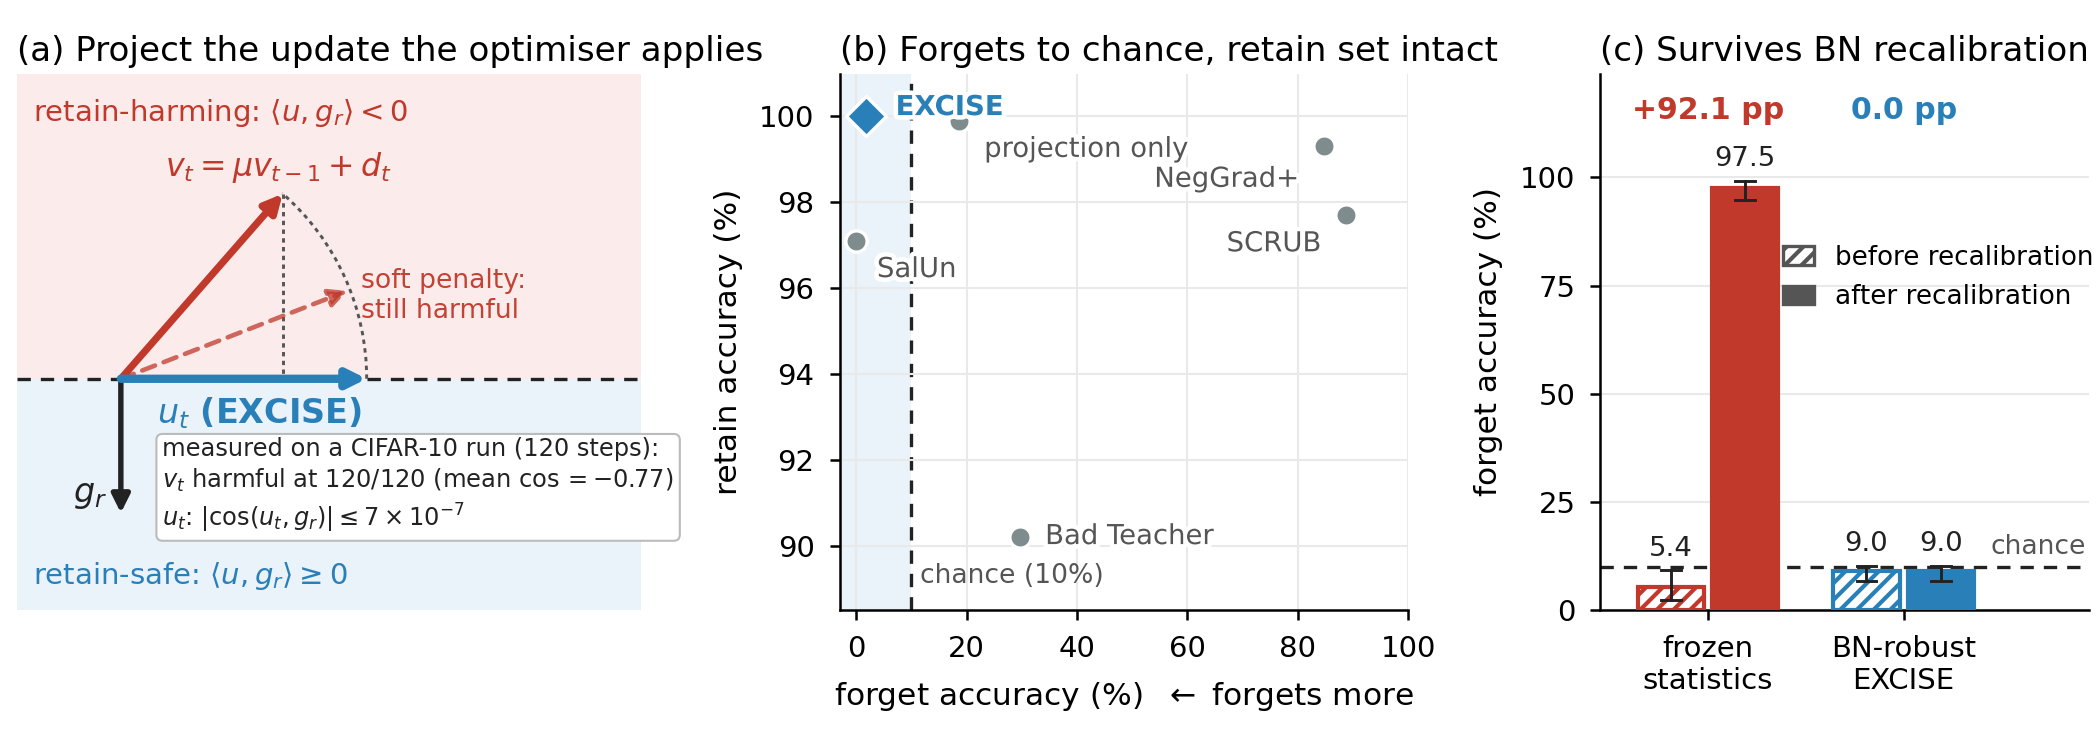
\includegraphics[width=\textwidth]{fig_teaser.png}
\caption{\rev{\textbf{\ours{} in one picture.} \textbf{(a)}~With momentum, the
update the optimiser applies is the accumulated $v_t$, and in unlearning it
points into the retain-harming half-space at every step. \ours{} projects $v_t$
onto the boundary and restores its length, so the applied $u_t$ cannot increase
the sampled retain loss to first order (Theorem~\ref{thm:retain_safety}); a
soft penalty only tilts the step, which stays harmful
(Theorem~\ref{thm:separation}). The boxed numbers are measured
(Figure~\ref{fig:guarantee}). \textbf{(b)}~On CIFAR-10 class~0, \ours{} is the
only method in Table~\ref{tab:cifar10} that forgets to chance with the retain
set intact. \textbf{(c)}~With frozen BatchNorm statistics, recomputing them on
retained data undoes the forgetting on every CIFAR-10 class; BN-robust \ours{}
does not move. Bars are means over the ten classes and whiskers their range
(Table~\ref{tab:app_bnrobust}).}}
\label{fig:teaser}
\end{figure}

\paragraph{The mirror image in continual learning.}
Continual learning (CL) faces the same problem with the sign reversed: learn a
new task while protecting old ones. \rev{One of its most direct answers} is not
a penalty but a \emph{constraint on the update}. A-GEM \citep{chaudhry2019agem} projects any
update $v$ with $\langle v, g_{\text{old}}\rangle < 0$ onto the half-space
$\{u : \langle u, g_{\text{old}}\rangle \ge 0\}$, so a step that would increase
old-task loss to first order is never taken. Unlearning lacks exactly this
guarantee: \rev{most} existing methods control retain damage with weighted
objectives, saliency masks or alternating updates (\S\ref{sec:related}), which
\rev{discourage retain-harming steps rather than exclude them}. We treat the retain set as CL's ``old task'' and
adopt the half-space constraint as the update rule for unlearning. The duality
has been noted before \citep{kurmanji2023unbounded,nguyen2020variational}, and
the forget--retain conflict has been targeted by a soft regulariser
\citep{patel2025learning}\added{ and by projecting updates away from a retain
gradient subspace \citep{hoang2024learn}}; what has not been done\rev{, to our
knowledge,} is to enforce the half-space constraint \rev{against the current
retain gradient}, at every step, on the vector the optimiser applies.

\paragraph{What it takes.}
Three design decisions \rev{complete the method}. \emph{Project the update, not
the gradient}: with momentum, the applied vector is the accumulated update, and
projecting the gradient certifies nothing about it
(Proposition~\ref{prop:counter}). Removing momentum would make the analysis
exact but \rev{leaves forget accuracy far above chance on five of six datasets}
(\S\ref{sec:momentum_ablation}), so we project the post-momentum update and make
the guarantee hold for the optimiser that runs. \emph{Push the forgotten class
toward the model's own retain-confusion distribution}, rather than the uniform
distribution no trained model produces\rev{; at equal test accuracy it forgets
further than gradient ascent and slightly further than a uniform target}
(\S\ref{sec:forget_obj}). \emph{Stop on explicit tolerances} for retain loss and
forget accuracy rather than on an epoch count (\S\ref{sec:stopping}).

\paragraph{Forgetting that survives the attack.}
A fourth issue came from the experiments. Forget batches contain a single
class and would corrupt BatchNorm running statistics, so the method freezes them
during unlearning---and the weights then learn to forget \emph{relative to}
statistics an attacker can replace: recomputing them on retained data restores
forget accuracy from ${\sim}1\%$ to ${\sim}100\%$ without changing a weight
(\S\ref{sec:bn_results}). \rev{The attack reaches beyond us. Concurrent work
\citep{kalani2026batchnorm} applies it to nine prior methods and recovers the
forgotten class for six of them; of the other three, gradient ascent forgets
only by destroying the model ($57\%$ retain accuracy), GA+FT does not forget
($68\%$ forget accuracy), and SCRUB keeps its forgetting at $88\%$ retain
accuracy. Whether a method survives depends less on the method than on how its
statistics are handled during unlearning: in \citet{kalani2026batchnorm},
mixing at least a quarter of retained data into SalUn's unlearning batches
removes its recovery, and our own reproductions of SalUn and Bad Teacher, which
end every epoch with a pass over retained data that recomputes the statistics,
are not recovered at all. BN-robust \ours{} makes survival a property of the
method rather than of how it is run: it keeps the statistics consistent with the
weights throughout unlearning, forgets to chance on every CIFAR-10 class and on
MNIST, survives the attack in every case we tried---including when the attacker
chooses the recalibration data---and keeps the per-step guarantee
(\S\ref{sec:bn_robust}). To our knowledge it is the only unlearning method for
BatchNorm ResNets whose survival has been verified on every class of a benchmark
and against attacker-chosen recalibration data, which we take to make it the
state of the art for this setting, pending a like-for-like run of the prior
methods under the same base and attack (\S\ref{sec:limitations}).}

\paragraph{Contributions.}
\textbf{(1)}~A constrained formulation of class unlearning
(Eq.~\ref{eq:problem}) \rev{that assigns each mechanism of the algorithm to the
condition it enforces}.
\textbf{(2)}~\ours{}: A-GEM projection as the \emph{update rule} of unlearning,
applied to the post-momentum update, with clipping before accumulation and
magnitude-preserving projection. \textbf{(3)}~An exact per-step retain-safety
theorem for that optimiser, a separation theorem showing that gradient ascent,
SCRUB, SalUn and soft conflict penalties admit retain-harming steps, and
\rev{tests of both theorems on real runs}. \textbf{(4)}~\rev{A
BatchNorm-recalibration failure mode of \ours{} and a fix that keeps BatchNorm,
verified on every CIFAR-10 class, on MNIST and against attacker-chosen
recalibration data.} We also show that the conventional MIA target of $0.5$ is
the wrong reference point for class unlearning (\rev{\S\ref{sec:mia_main}}).
\rev{Table~\ref{tab:claims} maps every claim to the experiment that tests it.}

% ============================================================
\section{Related Work}\label{sec:related}

\emph{Exact} unlearning retrains on shards \citep{bourtoule2021sisa} or certifies
removal for convex models \citep{guo2020certified}. \emph{Approximate} methods
modify the trained model: gradient ascent and NegGrad+ \citep{thudi2022unrolling}
maximise forget loss, the latter with a weighted retain term; SalUn
\citep{fan2024salun} confines random-label updates to a saliency mask; Fisher
methods and SSD \citep{golatkar2020eternal,foster2024ssd} dampen parameters by
estimated importance; Bad Teacher \citep{chundawat2023badteacher} and SCRUB
\citep{kurmanji2023unbounded} use distillation, SCRUB alternating forget and
retain steps. Each balances forgetting against retain damage through a weight, a
mask or a schedule, so retain damage is discouraged rather than excluded
(Theorem~\ref{thm:separation}). Closest to us are methods that address the
forget--retain gradient conflict directly: \citet{patel2025learning} with a soft
regulariser that rewards positive alignment, and \added{\citet{hoang2024learn}
by stepping orthogonally to a gradient subspace estimated for the retained
data}. \ours{} instead imposes A-GEM's half-space constraint
\citep{chaudhry2019agem} against the current retain gradient at every step, on
the post-momentum update the optimiser applies, which is what makes its guarantee
exact for the deployed optimiser. Table~\ref{tab:properties} summarises the structural
difference; Appendix~\ref{app:related} gives the full comparison. \rev{On the
evaluation side, \citet{kalani2026batchnorm} show that recomputing BatchNorm
statistics recovers the forgotten class for six of nine prior methods;
\S\ref{sec:bn_results} applies the same attack to \ours{}.}

\begin{table}[t]
\centering
\caption{\textbf{Structural comparison of update rules.} \cmark~= holds by
construction, \pmark~= partial or hyperparameter-dependent, \xmark~= not
provided. Entries are properties of each method's \emph{definition}, not
measured quantities; an empirical comparison against
\citet{patel2025learning} is future work (\S\ref{sec:limitations}).
P\&Q = \citet{patel2025learning}; \rev{PGU = \citet{hoang2024learn}, whose
projection removes the update's component in a retain subspace estimated before
unlearning and truncated at an energy threshold, so its protection is
approximate and not stated against the current retain gradient.}
$^\dagger$\ours{} takes an explicit tolerance and honours it across a $29$pp
range, but only when the stopping rule is evaluated per step: at a 50-batch
check granularity, targets from $5\%$ to $30\%$ collapse onto the same operating
point (\S\ref{sec:further}, Table~\ref{tab:sweeps}).}
\label{tab:properties}
\small
\begin{tabular}{@{}lccccccc@{}}
\toprule
\textbf{Property} & \textbf{GA} & \textbf{SalUn} & \textbf{SCRUB} &
\textbf{NG+} & \textbf{P\&Q} & \rev{\textbf{PGU}} & \textbf{\ours{}} \\
\midrule
Addresses forget--retain gradient conflict & \xmark & \xmark & \pmark & \pmark & \cmark & \cmark & \cmark \\
Conflict handled as a constraint, not a penalty & \xmark & \xmark & \xmark & \xmark & \xmark & \cmark & \cmark \\
Retain-harming steps are unreachable & \xmark & \xmark & \xmark & \xmark & \xmark & \pmark & \cmark \\
Per-step retain-safety guarantee & \xmark & \xmark & \xmark & \xmark & \xmark & \pmark & \cmark \\
Explicit forgetting tolerance & \xmark & \xmark & \pmark & \pmark & \pmark & \pmark & \cmark$^\dagger$ \\
Guarantee holds for the optimiser actually run & \xmark & \xmark & \xmark & \xmark & \xmark & \pmark & \cmark \\
\bottomrule
\end{tabular}
\end{table}

% ============================================================
\section{Problem Formulation}\label{sec:problem}

Let $f_\theta$ be a trained $K$-class classifier with weights $\theta_0$,
$\sigma$ the softmax, and $p_\theta(x) = \sigma(f_\theta(x))$. The training set
splits into a forget set $\Df$ and a retain set $\Dr$. We evaluate with test
accuracy (TA, held-out data), forget accuracy (FA, on $\Df$; a fully unlearned
model reaches at most the chance level $100/K\%$), retain accuracy (RA, on
$\Dr$), and the AUROC of a membership-inference attack (MIA) between forget-class
training and test samples. The \emph{retain-confusion distribution} is the base
model's average prediction on retained data,
\begin{equation}\label{eq:retain_confuse}
p_r = \frac{1}{|\Dr|}\sum_{x \in \Dr} \sigma(f_{\theta_0}(x)),
\end{equation}
and we pose unlearning as \rev{a constrained search: find
\begin{equation}\label{eq:problem}
\theta^\star \in \big\{\theta :\;
\mathrm{FA}(\theta;\Df) \le \tau_F,\;\;
\CE(\theta;\Dr) \le \alpha\,\CE(\theta_0;\Dr),\;\;
\|\theta - \theta_0\| \le R \big\},
\end{equation}
where $\tau_F$ is a forget-accuracy target (the chance level by default),
$\alpha \ge 1$ a tolerance on the retain loss, and $R$ a trust radius. The first
two conditions say what it means to have forgotten without damage; the third
asks for a solution near the trained model, and the search path supplies it.
\ours{} starts at $\theta_0$, descends the forget objective
$\lossf = \mathbb{E}_{x_f}[\KL(p_\theta(x_f)\|p_r)]$ along directions that do
not increase the retain objective
$\lossr = \mathbb{E}_{(x,y)}[\CE(f_\theta(x),y)] + \beta\,\losskd$ to first
order, where $\beta$ weights a distillation anchor, and returns the first point
that meets the forget target. $\lossf$ supplies the direction, not the
destination: driving it to its minimum over-forgets (Appendix~\ref{app:d2r}).
Retain safety is imposed at two levels. At every step the projection of
\S\ref{sec:projection} keeps the applied update in
$\{u : \langle u,\gr\rangle \ge 0\}$, so the sampled retain objective cannot
increase to first order (Theorem~\ref{thm:retain_safety}); on the full retain
set, the stopping rule ends the search if the retain cross-entropy exceeds its
tolerance. The first level is a hard constraint rather than a penalty because a
Lagrangian relaxation would turn it back into the soft treatment whose feasible
set still contains retain-harming steps (Theorem~\ref{thm:separation}(iv)). The
trust region needs no mechanism of its own: every step has length at most
$\eta c/(1-\mu)$ (Theorem~\ref{thm:retain_safety}), so $N$ steps stay within
$R = N\eta c/(1-\mu)$. Table~\ref{tab:constraint_map}
(Appendix~\ref{app:method}) maps each condition to its mechanism.}

% ============================================================
\section{The \ours{} Algorithm}\label{sec:method}

Algorithm~\ref{alg:excise} gives the update. Each step computes a retain gradient
$\gr$ on a retain mini-batch (cross-entropy plus the distillation anchor) and a
forget gradient $\gf$ on a forget mini-batch.

\begin{algorithm}[t]
\caption{\ours{} unlearning (projected-momentum update)}\label{alg:excise}
\begin{algorithmic}[1]
\REQUIRE Trained model $\theta$, forget set $\Df$, retain set $\Dr$;
         lr $\eta$, momentum $\mu$, clip $c$, weight decay $\lambda_{\mathrm{wd}}$;
         \rev{targets $\tau_F$, $\alpha$; check interval $m$}
\ENSURE Unlearned model $\theta^*$
\STATE $\theta_{\text{orig}} \leftarrow \text{freeze}(\text{copy}(\theta))$;\quad
       set all BatchNorm layers to \texttt{eval} mode
\STATE $p_r \leftarrow \frac{1}{|\Dr|}\sum_{x \in \Dr}\sigma(\theta_{\text{orig}}(x))$
\STATE $L_0 \leftarrow \CE(\theta,\Dr)$;\quad $v \leftarrow 0$
\FOR{epoch $=1$ to $T$}
  \FOR{$(x_f,y_f)$ in $\Df$}
    \STATE Sample $(x_r,y_r)$ from $\Dr$
    \STATE $\gr \leftarrow \nabla_\theta[\CE(f_\theta(x_r),y_r) + \beta\losskd]$
    \STATE $\gf \leftarrow \nabla_\theta\lossf(\theta;x_f)$
    \STATE $d \leftarrow \mathrm{clip}_c\!\big(\gf + \lambda_{\mathrm{wd}}\theta\big)$
           \hfill\textit{// clip BEFORE accumulation}
    \STATE $v \leftarrow \mu v + d$
           \hfill\textit{// momentum}
    \IF{$\langle v, \gr\rangle < 0$}
      \STATE $u \leftarrow v - \frac{\langle v,\gr\rangle}{\|\gr\|^2}\gr$;\quad
             $u \leftarrow u\,\|v\|/\|u\|$
             \hfill\textit{// project the update, rescale}
    \ELSE
      \STATE $u \leftarrow v$
    \ENDIF
    \STATE $\theta \leftarrow \theta - \eta u$
    \IF{\rev{every $m$ steps:} $\mathrm{FA}(\theta,\Df) \le \tau_F$}
      \STATE \textbf{return} $\theta$ \hfill\textit{\rev{// forget target met}}
    \ENDIF
  \ENDFOR
  \IF{$\CE(\theta,\Dr) > \alpha L_0$}
    \STATE \textbf{return} $\theta$ \hfill\textit{\rev{// retain tolerance exceeded}}
  \ENDIF
\ENDFOR
\RETURN $\theta^* \leftarrow \theta$
\end{algorithmic}
\end{algorithm}

\subsection{Projection onto the Retain-Safe Half-Space}\label{sec:projection}

When a candidate update $v$ satisfies $\langle v,\gr\rangle < 0$, moving along it
would increase the retain loss to first order, and we replace it by its
projection
\begin{equation}\label{eq:projection}
\Pi_{\gr}(v) = v - \frac{\langle v,\gr\rangle}{\|\gr\|^2}\,\gr,
\qquad \langle \Pi_{\gr}(v),\gr\rangle = 0 .
\end{equation}
This is A-GEM's operator: the minimum-norm correction that restores
feasibility, at the cost of one extra backward pass. What changes is its role.
In A-GEM it occasionally corrects a process whose objective already points the
right way; in unlearning, erasing a class and keeping the rest are directly
opposed, and the projection fires at \rev{$96$--$100\%$ of steps in every \ours{}
run we logged} (\S\ref{sec:guarantee_measured}). It becomes the optimiser's defining step rather
than a safeguard, which has three consequences for how it must be applied.

\subsection{Which Vector to Project}\label{sec:optimiser}

\emph{(i) Project the update, not the gradient.} \ours{} uses SGD with momentum
$\mu$, weight decay and clipping $c$. The vector applied to the weights is the
accumulated update, so we accumulate first and project afterwards
(Algorithm~\ref{alg:excise}, lines 10--15); projecting $\gf$ instead leaves the
applied update unconstrained (Proposition~\ref{prop:counter},
Figure~\ref{fig:projorder}). \emph{(ii) Clip before accumulating.} Clipping the
per-step ingredient keeps momentum's $1/(1-\mu)$ amplification and gives
$\|v_t\| \le c/(1-\mu)$; clipping the final update would cap it at $c$\rev{,
the step size of the momentum-free update, which leaves forget accuracy far
above chance on five of six datasets (\S\ref{sec:momentum_ablation},
Proposition~\ref{prop:clip}). Raw forget gradients are ${\sim}100\times$ the
clip threshold, so clipping is always active and that cap would always bind.}
\emph{(iii) Preserve magnitude.} Projection shrinks the update by
$\sin\vartheta$, which vanishes when forget and retain gradients are nearly
opposed \rev{(on the logged CIFAR-10 run it falls to $0.37$)}, so we rescale the
projected update to the pre-projection norm; $\langle u_t,\gr\rangle = 0$ is
unaffected.

\begin{figure}[t]
\centering
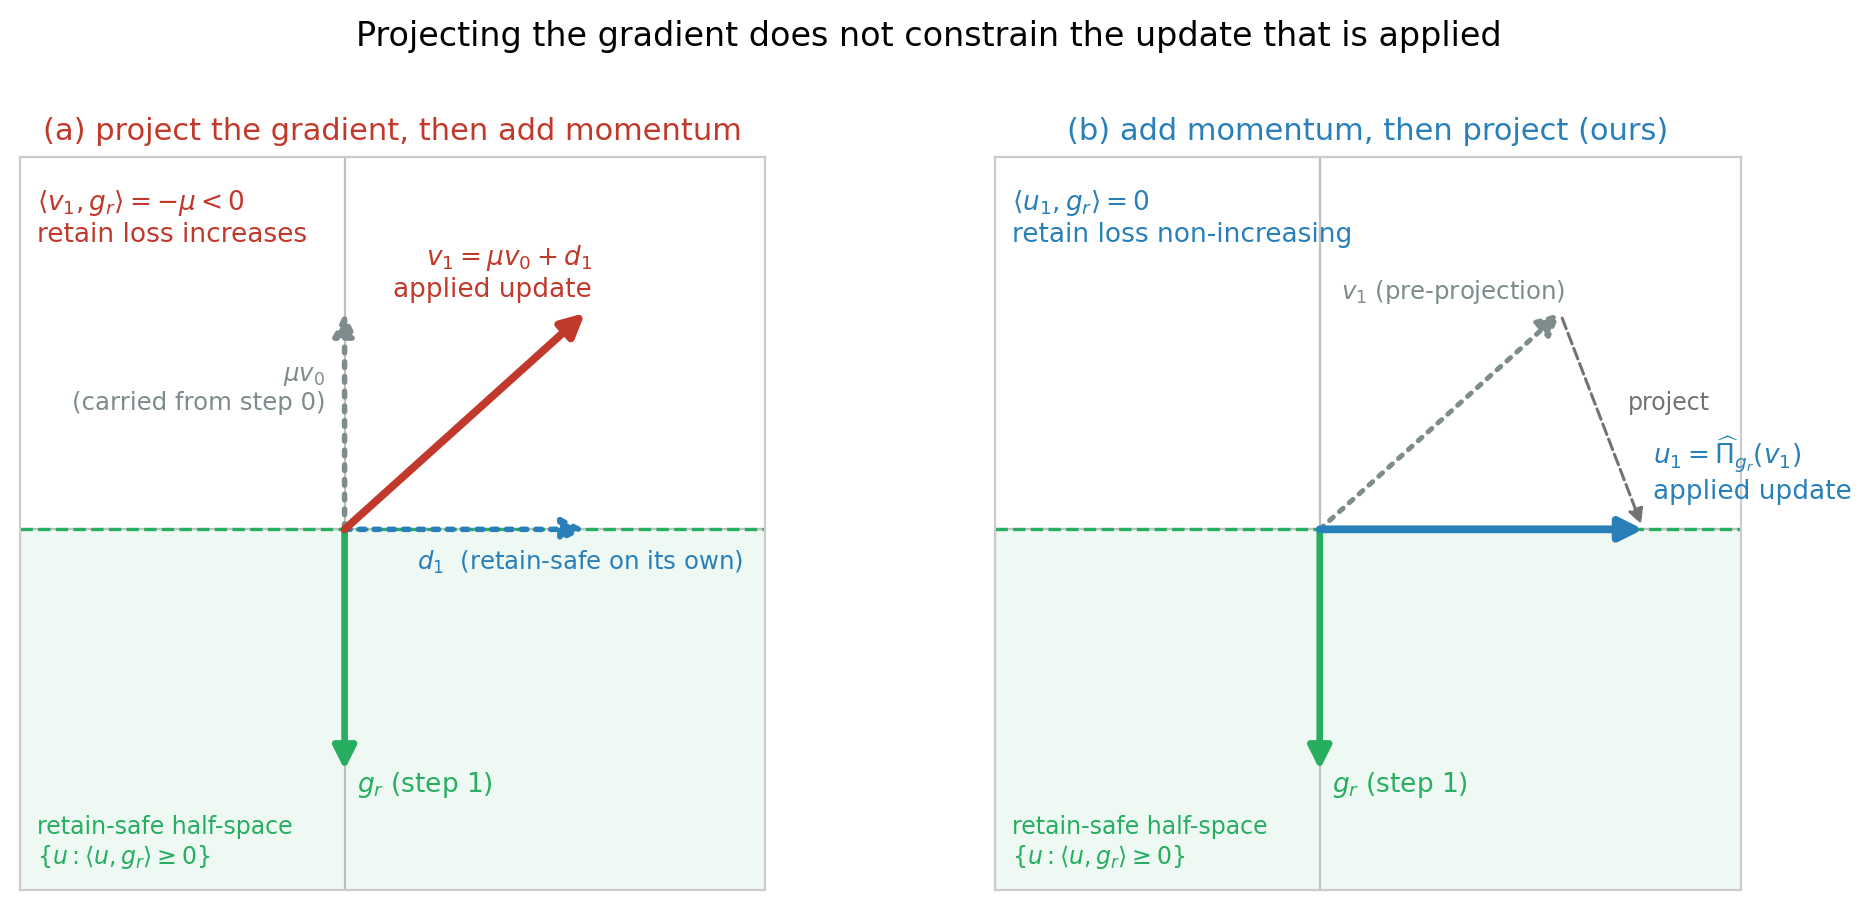
\includegraphics[width=0.86\textwidth]{fig_projection_order.png}
\caption{\textbf{Why the projection is applied to the update, not the
gradient} (Proposition~\ref{prop:counter}). Both panels show step~1, whose
constraint is $\gr$; the retain-safe half-space is shaded. \textbf{(a)}~Each
ingredient is individually retain-safe---$d_1$ lies on the boundary, and
$\mu v_0$ was certified against step~0's constraint---yet their sum, the vector
actually applied, lies in the harming half-space with
$\langle v_1,\gr\rangle = -\mu$. The violation grows with $\mu$.
\textbf{(b)}~Projecting the accumulated update instead returns it to the
boundary, so the certificate is issued against the constraint in force where
the step is taken.}
\label{fig:projorder}
\end{figure}

\subsection{Forget Objective, Stopping, and Normalisation}\label{sec:forget_obj}

The \klr{} objective drives forget-set predictions toward the retain-confusion
distribution rather than the uniform one,
\begin{equation}\label{eq:kl_retain}
\mathcal{L}_{\text{KL-R}} = \KL\!\left(\log\sigma(f_\theta(x_f)) \,\|\, p_r\right).
\end{equation}
Under the projected-momentum optimiser it forgets further than gradient ascent
\rev{and slightly further than a uniform target at equal test accuracy (FA
$2.1\%$ against $8.2\%$ and $3.9\%$, at TA $86.1$, $86.4$ and $86.4\%$; CIFAR-10
class~0, one seed)} and is within noise of a uniform target on MIA, so we claim a
better forget \emph{direction}, not a closer imitation of a retrained model
(Appendix~\ref{app:method}).

\paragraph{Dual stopping.}\label{sec:stopping}
Unlearning halts if the retain \rev{cross-entropy, measured on the full retain
set after each epoch,} exceeds $\alpha$ times its initial value, and completes
when FA reaches \rev{the target $\tau_F$}---by default the chance level
$100/K\%$---checked \rev{every $m=50$ steps} within epochs, because FA can fall
by tens of points inside one.

\paragraph{BatchNorm.}\label{sec:bn}
Class-homogeneous forget batches would corrupt BatchNorm running statistics, so
\ours{} freezes them. \added{The weights then learn to forget relative to those
frozen statistics; \S\ref{sec:bn_results} shows that this forgetting does not
survive recomputing them, and BN-robust \ours{} recomputes them from retained
data before every step instead (\S\ref{sec:bn_robust}).} A distillation anchor to
the frozen base model \rev{enters the retain objective; removing it changes
retain accuracy by only $0.04$pp on CIFAR-10 (\S\ref{sec:guarantee_measured}),
so we keep it as a safeguard rather than claim it as load-bearing}.

% ============================================================
\section{Theoretical Guarantees}\label{sec:theory}

\begin{theorem}[Exact per-step retain safety under momentum]\label{thm:retain_safety}
Let \rev{$\Lrt$, the retain objective $\lossr$ (cross-entropy plus
$\beta\losskd$) evaluated on the sampled retain mini-batch,} be $L$-smooth, and
let $\gr = \nabla_\theta\Lrt(\theta_t)$. Let \ours{} run the update of
Algorithm~\ref{alg:excise}: $\|d_t\| \le c$ by clipping,
$v_t = \mu v_{t-1} + d_t$ with $v_{-1}=0$ and $\mu \in [0,1)$,
$u_t = \Pi_{\gr}(v_t)\,\|v_t\|/\|\Pi_{\gr}(v_t)\|$ when
$\langle v_t,\gr\rangle<0$ \rev{(and $u_t=0$ if $\Pi_{\gr}(v_t)=0$)} and
$u_t = v_t$ otherwise, and $\theta_{t+1} = \theta_t - \eta u_t$. Then, exactly
and \rev{with no assumption on $\gf$ or on its alignment with $\gr$},
\begin{equation}\label{eq:thm1}
\langle u_t,\gr\rangle \ge 0,
\qquad \|u_t\| \;\rev{\le}\; \|v_t\| \;\le\; \frac{c}{1-\mu},
\qquad \Lrt(\theta_{t+1}) \;\le\; \Lrt(\theta_t) + \tfrac{1}{2}L\eta^2\Big(\frac{c}{1-\mu}\Big)^{\!2}.
\end{equation}
\end{theorem}

\begin{proof}[Proof sketch]
The first claim is immediate: if $\langle v_t,\gr\rangle \ge 0$ then $u_t=v_t$;
otherwise $\langle \Pi_{\gr}(v_t),\gr\rangle = 0$ identically, and rescaling by
a positive scalar preserves this. For the second, $\Pi_{\gr}$ is the orthogonal
projection onto $\{u : \langle u,\gr\rangle = 0\}$, so the rescaling restores
$\|u_t\|=\|v_t\|$ \rev{unless the projection vanishes}; unrolling the buffer gives
$v_t = \sum_{k=0}^{t}\mu^{t-k}d_k$, hence
$\|v_t\| \le c\sum_{j=0}^{t}\mu^{j} < c/(1-\mu)$. The third follows from
$L$-smoothness,
$\Lrt(\theta_{t+1}) \le \Lrt(\theta_t) - \eta\langle u_t,\gr\rangle
+ \tfrac{1}{2}L\eta^2\|u_t\|^2$, where the first-order term is non-positive by
claim one and $\|u_t\|$ is bounded by claim two. The full proof, together with the three supporting lemmas, is given in Appendix~\ref{app:thm1} (Theorem~\ref{thm:app_main}).
\end{proof}

The first-order change in the sampled retain loss is non-positive at every step,
and, unlike guarantees stated for momentum-free surrogates, the analysed $u_t$ is
the vector the code applies. The bound concerns the sampled mini-batch objective,
not the population retain loss (\S\ref{sec:limitations}).
\rev{Section~\ref{sec:guarantee_measured} tests the theorem on a logged run.}

\begin{theorem}[Per-step separation]\label{thm:separation}
For any model $\theta_0$ with retain gradient $\gr$:
\textbf{(i)}~GA's update $+\eta\gf$ strictly increases retain loss to first
order whenever $\langle\gf,\gr\rangle>0$;
\textbf{(ii)}~SCRUB's $-\gf+\lambda\gr$ can have $\langle\cdot,\gr\rangle<0$ for
any fixed $\lambda$;
\textbf{(iii)}~SalUn's masked random-label gradient has unconstrained sign with
respect to $\gr$;
\textbf{(iv)}~a soft conflict regulariser that adds $\rho\,\phi(\langle
g,\gr\rangle)$ with $\phi$ decreasing---the approach of the closest prior work
\citep{patel2025learning}---shifts the optimum toward positive alignment but
leaves the feasible set unrestricted: for any finite $\rho$, a sufficiently
large forget-loss reduction still makes a step with $\langle g,\gr\rangle<0$
preferable.
\rev{Among these update rules, only \ours{}'s} guarantees
$\langle u_t,\gr\rangle \ge 0$ \rev{at every step}, because only a projection
makes such steps unreachable rather than merely costly.
\end{theorem}

% ============================================================
\section{Experiments}\label{sec:experiments}

\subsection{Setup}\label{sec:setup}

We forget one class at a time on six benchmarks that vary class count, examples
per class and domain: CIFAR-10 and CIFAR-100 \citep{krizhevsky2009cifar}, MNIST
\citep{lecun1998mnist}, SVHN \citep{netzer2011svhn}, STL-10
\citep{coates2011stl10} and PathMNIST \citep{yang2023medmnist}. We forget every
class of MNIST and PathMNIST, \rev{classes $10, 20, \dots, 90$ of CIFAR-100}, and
class~0 of CIFAR-10, SVHN and STL-10 over three seeds: 31 tasks and 75 runs. All
models are ResNet-18 \citep{he2016resnet}. \rev{SalUn, SCRUB, Bad Teacher and
NegGrad+ are re-run on our stack, and a model retrained without the forget class
serves as the reference. MIA is the mean AUROC of a loss and a confidence
attack.} Hyperparameters are fixed per dataset and released as configuration
files (Appendix~\ref{app:hyper}); Appendix~\ref{app:experiments} gives the full
protocol. \rev{Table~\ref{tab:claims} lists every claim of \S\ref{sec:intro}
with the experiment that tests it; the subsections follow its order.}

\begin{table}[t]
\centering\color{revisedB}
\caption{\rev{\textbf{Each claim and the experiment that tests it.}}}
\label{tab:claims}
\small
\renewcommand{\arraystretch}{1.08}
\begin{tabular}{@{}>{\raggedright\arraybackslash}p{0.28\textwidth}>{\raggedright\arraybackslash}p{0.26\textwidth}>{\raggedright\arraybackslash}p{0.40\textwidth}@{}}
\toprule
\textbf{Claim} & \textbf{Test} & \textbf{Outcome} \\
\midrule
Forgets to chance, retain set intact & 31 tasks, six datasets (Table~\ref{tab:cross}) & Chance on all six, two at 60 epochs; RA $\ge 97.2\%$ on the 10-class datasets \\
Only \ours{} does both on CIFAR-10 & Four baselines, projection only (Table~\ref{tab:cifar10}) & FA $1.87\%$ at RA $100\%$; SalUn loses $2.9$pp RA, the rest stop at FA $\ge 18.7\%$ \\
Theorem~\ref{thm:retain_safety} holds for the optimiser that runs & Step-level audit (Figure~\ref{fig:guarantee}) & $120/120$ steps conflict before projection; $|\cos| \le 7.4\times10^{-7}$ after; $\|u_t\| \le 9.16 < 10$ \\
Soft corrections leave harm reachable (Thm.~\ref{thm:separation}) & Projection strength $s$, equal compute (\S\ref{sec:guarantee_measured}) & RA rises from $52.5$ to $99.98\%$ as $s \to 1$; every $s<1$ leaves conflict in the applied step \\
The projection protects the retain set & Ablation, equal compute (\S\ref{sec:guarantee_measured}) & Without it RA is $52.6\%$; alone it keeps RA $99.9\%$ but stops at FA $18.7\%$ \\
The guarantee must cover momentum & $\mu = 0$ ablation (Table~\ref{tab:momentum}) & With $\mu=0$, FA stays far above chance on five of six datasets \\
Frozen statistics make forgetting reversible & Recalibration attack (Table~\ref{tab:bnrecal}) & Frozen \ours{}: FA $1.4 \to 99.7\%$; base model and our baselines: $\Delta F \le 0$ \\
BN-robust \ours{} survives it & Ten classes, MNIST, attacker's data (Figures~\ref{fig:teaser}c, \ref{fig:bnrobust_attack}) & $|\Delta F| \le 0.06$pp on every CIFAR-10 class, $+0.09$pp on MNIST; attacker's data: $-1.2$ to $-1.0$pp \\
$0.5$ is the wrong MIA target & Retrained references (Table~\ref{tab:mia_main}) & References score $0.69$ (CIFAR-10) and $0.31$--$0.70$ (PathMNIST); rankings reverse \\
$p_r$ is a better direction than uniform & Forget objectives, equal TA (\S\ref{sec:forget_obj}) & FA $2.1\%$ against $3.9\%$ (uniform) and $8.2\%$ (GA); one seed \\
\bottomrule
\end{tabular}
\end{table}

\subsection{Main Results}\label{sec:main_results}

\begin{table}[t]
\centering
\caption{\textbf{Cross-dataset results.} Mean $\pm$ \rev{sample} std over
classes $\times$ seeds (3 seeds \rev{per task; one seed per class for
CIFAR-100}). \#T = number of forgetting tasks. Chance $=100/K\%$ is the level a
fully unlearned model must reach. \rev{The upper block uses each dataset's epoch
cap (12--20 epochs, Appendix~\ref{app:hyper}), which penalises datasets with few
images per class, since the binding resource is optimiser steps rather than
epochs. The lower block re-runs the two datasets that fall short at 60 epochs
($4\times$ and $3\times$ their caps), with a per-step check and a $1\%$ forget
target,} on the same seeds and classes;
$^*$marks the STL-10 row it supersedes (\S\ref{sec:crossdataset_stl}).}
\label{tab:cross}
\begin{tabular}{@{}lccccccc@{}}
\toprule
\textbf{Dataset} & \textbf{\#T} & \textbf{Chance} & \textbf{TA} & \textbf{FA}$\downarrow$ & \textbf{RA} & \textbf{MIA} \\
\midrule
CIFAR-10    & 1 & 10.0\% & $86.13 \pm 0.02$ & $\mathbf{1.87} \pm 0.25$ & $100.00 \pm 0.00$ & $0.529 \pm 0.001$ \\
MNIST       & 10 & 10.0\% & $90.00 \pm 0.64$ & $\mathbf{6.17} \pm 2.81$ & $99.49 \pm 0.04$ & $0.497 \pm 0.009$ \\
SVHN        & 1 & 10.0\% & $89.69 \pm 0.02$ & $\mathbf{5.75} \pm 0.17$ & $97.26 \pm 0.01$ & $0.525 \pm 0.001$ \\
STL-10$^*$  & 1 & 10.0\% & $92.84 \pm 0.02$ & $75.67 \pm 1.70$ & $99.38 \pm 0.10$ & $0.466 \pm 0.005$ \\
PathMNIST   & 9 & 11.1\% & $80.96 \pm 5.39$ & $\mathbf{5.82} \pm 3.42$ & $98.88 \pm 0.31$ & $0.483 \pm 0.084$ \\
CIFAR-100   & 9 & \phantom{0}1.0\% & $76.17 \pm 0.86$ & $4.07 \pm 5.51$ & $92.19 \pm 0.84$ & $0.500 \pm 0.037$ \\
\midrule
\multicolumn{7}{@{}l}{\emph{Extended budget} (\rev{60 epochs, per-step check, $1\%$ forget target}; same seeds and classes)} \\
STL-10      & 1 & 10.0\% & $85.15 \pm \rev{0.06}$ & $\mathbf{1.73} \pm \rev{0.95}$ & $98.87 \pm \rev{0.05}$ & $\rev{0.488} \pm \rev{0.008}$ \\
CIFAR-100   & 9 & \phantom{0}1.0\% & $75.50 \pm \rev{0.68}$ & $\mathbf{1.27} \pm \rev{0.39}$ & $91.32 \pm \rev{0.94}$ & $\rev{0.490} \pm \rev{0.043}$ \\
\bottomrule
\end{tabular}
\end{table}

\begin{table}[t]
\centering
\caption{\textbf{CIFAR-10 class-0 forgetting.} \ours{} is a 3-seed mean $\pm$
std. Methods with FA~$>80\%$ attain MIA~$\approx 0.5$ trivially, by barely
changing the model. $\dagger$Our reproduction; $\ddagger$our reproduction with
unified MIA. $^\S$A-GEM projection applied to plain gradient ascent, with
\ours{}'s KD anchor and retain-confusion target removed: the direct
projected-gradient baseline, isolating what the projection alone achieves.
\rev{$^\P$The retrained reference of \S\ref{sec:mia_main}; its TA and RA were
not logged, and its MIA, from the same two attacks, is $0.565$, not $0.5$.}}
\label{tab:cifar10}
\begin{tabular}{@{}lcccc@{}}
\toprule
\textbf{Method} & \textbf{TA} & \textbf{FA}$\downarrow$ & \textbf{RA} & \textbf{MIA} \\
\midrule
\rev{Retrain (reference)$^\P$} & \rev{---} & 0.0 & \rev{---} & \rev{0.565} \\
\midrule
SalUn$^\dagger$        & 84.0 & 0.0  & 97.1 & 0.497 \\
Bad Teacher$^\ddagger$ & 82.0 & 29.7 & 90.2 & 0.499 \\
SCRUB$^\ddagger$       & 93.3 & 88.8 & 97.7 & 0.515 \\
NegGrad+$^\ddagger$    & 94.2 & 84.8 & 99.3 & 0.525 \\
\midrule
Projection-only$^\S$   & 86.23 & 18.66 & 99.90 & 0.511 \\
\midrule
\textbf{\ours{}} & $\mathbf{86.13}\pm.02$ & $\mathbf{1.87}\pm.25$ & $\mathbf{100.00}\pm.00$ & $\mathbf{0.529}\pm.001$ \\
\bottomrule
\end{tabular}
\end{table}

\rev{At its epoch cap} \ours{} drives FA to or below the chance level on four
of six datasets with RA $\ge 97.2\%$ (CIFAR-100: $92.2\%$), and \rev{the mean
over seeds is below chance for every one of the ten MNIST and nine PathMNIST
classes (one of the 30 MNIST runs ends at $10.2\%$, within sampling error)}
(Table~\ref{tab:cross}, Appendix~\ref{app:perclass}). The two shortfalls are
budget-limited: STL-10 gets ${\sim}60$ optimiser steps at \rev{its 15-epoch cap}
against ${\sim}600$ for CIFAR-10 \rev{at the same cap}, and at 60 epochs
\rev{(per-step check, $1\%$ target)} STL-10 reaches $1.73\%$ \rev{($9.2\%$ in a
single run at its default $10\%$ target)} and CIFAR-100 $1.27\%$\rev{---against a $1\%$ chance level,
within one standard error of a 500-image forget set}---so all six datasets reach
chance. On CIFAR-10 (Table~\ref{tab:cifar10}, \rev{Figure~\ref{fig:teaser}b}),
\ours{} is the only method \rev{in the table} that both forgets to chance
and leaves retain accuracy untouched: SalUn forgets fully but costs $2.9$pp of
retain accuracy, Bad Teacher stops at $29.7\%$ while damaging the model, and
SCRUB and NegGrad+ keep the model intact by barely forgetting. The projection
alone does not unlearn: applied to plain gradient ascent it preserves the retain
set but stalls at $18.66\%$, so the projection supplies retain safety and the
\klr{} objective supplies the forgetting.

\subsection{The Guarantees, Measured}\label{sec:guarantee_measured}

\begin{figure}[t]
\centering
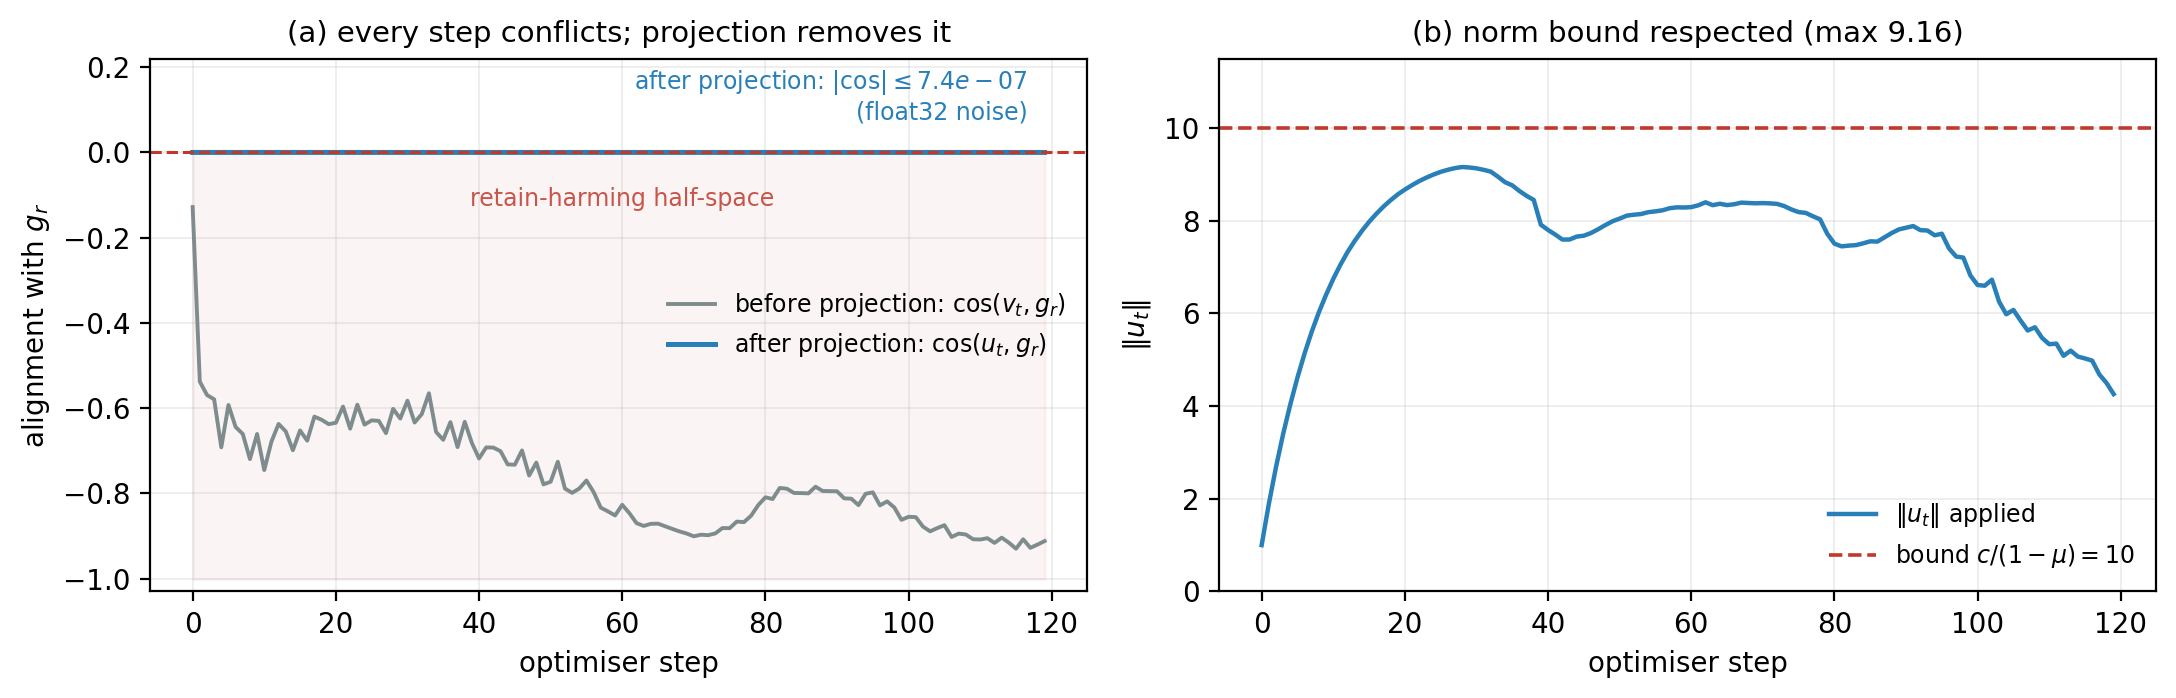
\includegraphics[width=0.86\textwidth]{fig_guarantee.png}
\caption{\textbf{Theorem~\ref{thm:retain_safety} audited on a real run}
(CIFAR-10 class~0, 120 steps). \textbf{(a)}~Alignment with the retain gradient,
normalised to $\cos(\cdot,\gr)$. Before projection every step lies in the
retain-harming half-space (mean $-0.77$); after projection the alignment is
indistinguishable from zero ($|\cos| \le 7.4\times10^{-7}$, the float32
accumulation scale). \textbf{(b)}~The applied update never exceeds the bound
$c/(1-\mu)=10$ of Eq.~\ref{eq:thm1}, peaking at $9.16$---tight, but respected.}
\label{fig:guarantee}
\end{figure}

\rev{\paragraph{Theorem~\ref{thm:retain_safety} on a real run.}
We log every step of a CIFAR-10 run (class~0, 120 steps;
Figure~\ref{fig:guarantee}, Appendix~\ref{sec:alignment}). The accumulated update
conflicts with the retain gradient at all 120 steps (mean
$\cos(v_t,\gr) = -0.77$), so the projection is the optimiser's defining step
rather than a safeguard. After projection the alignment is zero to float32
precision ($|\cos(u_t,\gr)| \le 7.4\times10^{-7}$), and $\|u_t\|$ peaks at
$9.16$ against the bound $c/(1-\mu)=10$.

\paragraph{Theorem~\ref{thm:separation}(iv): soft against hard.}
To test the separation without reimplementing another method, we vary our own
projection between a soft correction and the hard constraint: at conflicting
steps $u = v - s\,\frac{\langle v,\gr\rangle}{\|\gr\|^2}\gr$, so
$\langle u,\gr\rangle = (1-s)\langle v,\gr\rangle < 0$ for every $s<1$. At equal
compute with stopping disabled every setting forgets completely (FA $0.0\%$), so
the settings differ only in collateral damage: RA is $52.5$, $81.4$, $92.8$,
$98.2$ and $99.98\%$ for $s = 0, 0.25, 0.5, 0.75, 1$ (Appendix~\ref{sec:strength}).
The curve is gradual---$s=0.75$ already keeps $98.2\%$---so the case for $s=1$
is that it is the only setting with a guarantee, not that the last $1.8$pp is
large.

\paragraph{The projection is what protects the retain set.}
At equal compute with stopping disabled, removing the projection collapses the
model (TA $44.4\%$ and RA $52.6\%$, against $85.7\%$ and $99.98\%$ with it),
removing the distillation anchor changes RA by $0.04$pp, and the projection on
its own keeps RA at $99.9\%$ but stalls at FA $18.7\%$
(Tables~\ref{tab:cifar10} and~\ref{tab:ablation}). With stopping enabled every
variant halts after one epoch and the projection looks costless, which is why we
report both modes.}

\subsection{Momentum Is Not Incidental}\label{sec:momentum_ablation}

\begin{table}[t]
\centering
\caption{\textbf{Momentum ablation.} Removing momentum to simplify the analysis
\rev{leaves forget accuracy far above chance on five of six datasets; on STL-10
projected momentum also falls short at this budget (Table~\ref{tab:cross})}.
High RA with high FA indicates the model barely changed. Same configs, seeds,
and stopping rules throughout.}
\label{tab:momentum}
\begin{tabular}{@{}lccccc@{}}
\toprule
& & \multicolumn{2}{c}{$\mu=0$ (analysis-friendly)} & \multicolumn{2}{c}{Projected momentum (ours)} \\
\cmidrule(lr){3-4}\cmidrule(lr){5-6}
\textbf{Dataset} & \textbf{Chance} & \textbf{FA}$\downarrow$ & \textbf{RA} & \textbf{FA}$\downarrow$ & \textbf{RA} \\
\midrule
CIFAR-10  & 10.0\% & \phantom{0}5.8 & 100.0 & \phantom{0}1.9 & 100.0 \\
MNIST     & 10.0\% & 95.9 & \phantom{0}99.5 & \phantom{0}6.2 & 99.5 \\
SVHN      & 10.0\% & 61.9 & \phantom{0}97.4 & \phantom{0}5.8 & 97.3 \\
STL-10    & 10.0\% & 99.7 & \phantom{0}99.4 & 75.7 & 99.4 \\
PathMNIST & 11.1\% & 16.4 & \phantom{0}99.0 & \phantom{0}5.8 & 98.9 \\
CIFAR-100 & \phantom{0}1.0\% & 73.7 & \phantom{0}94.1 & \phantom{0}4.1 & 92.2 \\
\bottomrule
\end{tabular}
\end{table}

Removing momentum is the most direct route to an exact guarantee, since the
applied update then equals the projected gradient. Table~\ref{tab:momentum} shows
the cost: with $\mu = 0$ and everything else fixed, \rev{forget accuracy stays
far above chance on five of six datasets} (FA $95.9\%$ on MNIST, $99.7\%$ on
STL-10, $73.7\%$ on CIFAR-100), and RA stays high only because the model barely
moves. \rev{STL-10 does not forget at this budget with momentum either
($75.7\%$), so the comparison rests on the other four: without momentum all four
stay far above chance; with it, three reach chance and CIFAR-100 ends at
$4.1\%$.} A guarantee stated for the momentum-free update would be exact and
would describe a method that does not unlearn. The dependence is not ours alone:
every update rule we tested loses forgetting without momentum, but the KL
objectives lose $70$--$79$pp against $12$--$15$pp for gradient ascent \rev{(with
or without projection; means over MNIST and SVHN), consistent with a bounded
objective needing} momentum's $1/(1-\mu)$ amplification
(Appendix~\ref{app:momentum}).

\subsection{BatchNorm: the Attack, and a Fix That Keeps BatchNorm}\label{sec:bn_results}

\begin{table}[t]
\centering
\caption{\textbf{BatchNorm recalibration} (CIFAR-10, class~0), using
\texttt{update\_bn} on the retain set: BatchNorm buffers are reset and
recomputed, no weight is touched. \rev{Our reproductions of the baselines}
and the un-unlearned base model are unaffected ($\Delta F \le 0$); \ours{} with a
BatchNorm backbone loses essentially all of its forgetting. The two backbones without running statistics
are outside the operator's reach by construction. NegGrad+ is omitted: no
checkpoint for it was available.}
\label{tab:bnrecal}
\begin{tabular}{@{}lccccc@{}}
\toprule
Configuration & pre-$F$ & post-$F$ & $\boldsymbol{\Delta F}$ & pre-TA & post-TA \\
\midrule
Base model (no unlearning)  & $100.0$ & $99.8$ & $-0.2$ & $95.5$ & $92.9$ \\
SalUn                       & $0.0$   & $0.0$  & $+0.0$ & $84.7$ & $84.4$ \\
Bad Teacher                 & $28.7$  & $28.4$ & $-0.3$ & $81.5$ & $84.0$ \\
SCRUB                       & $89.3$  & $85.7$ & $-3.6$ & $93.5$ & $93.2$ \\
\midrule
\ours{} (BatchNorm, frozen) & $1.4$   & $99.7$ & $\mathbf{+98.4}$ & $86.1$ & $92.9$ \\
\ours{} (GroupNorm)         & $4.9$   & $4.9$  & $\mathbf{0.0}$   & $84.2$ & $84.2$ \\
\ours{} (ViT-B/16, LayerNorm) & $9.6$ & $9.6$  & $\mathbf{0.0}$   & $87.0$ & $87.0$ \\
\bottomrule
\end{tabular}
\end{table}

\begin{table}[t]
\centering\color{revised}
\caption{\added{\textbf{BN-robust \ours{} under BatchNorm recalibration} (CIFAR-10,
class~0, seeds $\{42,123,456\}$; \texttt{update\_bn} on the retain set, as in
Table~\ref{tab:bnrecal}). Every row shares the $93.97\%$ base except GroupNorm,
which needs its own. The un-unlearned base is the control: recalibrating it
changes nothing. \emph{Naive} stopping reads FA under the in-loop statistics,
\emph{calibrated} stopping under the statistics that ship. Time is wall-clock per
run on one GPU.}}
\label{tab:bnrobust}
\small
\setlength{\tabcolsep}{4pt}
\begin{tabular}{@{}lcccccccc@{}}
\toprule
Configuration & base TA & pre-$F$ & post-$F$ & $\boldsymbol{\Delta F}$ & TA & RA & epochs & min \\
\midrule
Base model (no unlearning)     & $93.97$ & $99.80$ & $99.82$ & $+0.0$ & $93.97$ & ---     & ---          & ---    \\
\ours{} (BatchNorm, frozen)    & $93.97$ & $8.51 \pm 0.30$  & $99.12 \pm 0.09$ & $\mathbf{+90.6}$ & $85.20$ & $97.34$ & $2$          & $1.9$  \\
\ours{} (GroupNorm)            & $91.89$ & $5.91 \pm 0.09$  & n/a              & n/a              & $83.13$ & $98.92$ & $3$          & $2.5$  \\
BN-robust, naive stopping      & $93.97$ & $11.43 \pm 1.90$ & $11.44 \pm 1.87$ & $\mathbf{0.0}$   & $84.42$ & $95.46$ & $11$--$13$   & $9.8$  \\
BN-robust, calibrated stopping & $93.97$ & $9.19 \pm 0.08$  & $9.18 \pm 0.07$  & $\mathbf{0.0}$   & $84.30$ & $95.59$ & $13$         & $13.3$ \\
\bottomrule
\end{tabular}
\end{table}

\paragraph{The attack.}
\texttt{update\_bn} resets every BatchNorm buffer and recomputes the statistics
on the retain set without touching a weight; we verify that every learnable
parameter is bit-identical afterwards. Table~\ref{tab:bnrecal} shows that
recalibration leaves the un-unlearned base model and every baseline we
reproduced unaffected, but undoes \ours{} with frozen statistics completely:
forget accuracy returns from $1.4\%$ to $99.7\%$ and test accuracy to $92.9\%$,
\rev{the value recalibration gives the base model itself}. Because the
statistics are frozen, the weights learn to forget against statistics an
attacker can replace. \rev{Our baseline reproductions survive because each ends
every epoch with a pass over retained data in train mode, which recomputes the
statistics. Under their reference implementations, \citet{kalani2026batchnorm}
recover six of nine prior methods, and find SalUn's recovery disappears once at
least a quarter of each unlearning batch is retained data.} GroupNorm and a ViT's
LayerNorm keep no running statistics and are outside the attack's reach by
construction (Tables~\ref{tab:gn} and~\ref{tab:vit}), but that is a change of
architecture, not robustness.

\paragraph{BN-robust \ours{}.}\label{sec:bn_robust}
\added{We keep BatchNorm and stop the statistics going stale. Before every step
they are recomputed on 512 retain images with the attacker's own operator, after
the last step on the whole retain set, and the stopping rule reads forget
accuracy under the statistics that will ship, falling back to the best epoch if
the target is not met (\rev{Figure~\ref{fig:bnrobust_mech}, Appendix~\ref{app:bn_robust}}). The update rule is
unchanged, \rev{so Theorem~\ref{thm:retain_safety} holds at every step for the
retain objective under the statistics in force during that step; the
recalibration between steps is not a gradient step, and the theorem does not
bound its effect}. Table~\ref{tab:bnrobust} gives the
result on a separate base model (the checkpoints behind Table~\ref{tab:bnrecal}
were no longer available): with frozen statistics the attack returns forget
accuracy to $99.1\%$, while BN-robust \ours{} forgets to $9.2\%$ and stays at
$9.2\%$. It holds on all ten CIFAR-10 classes ($6.7$--$10.2\%$ after the attack,
all within three standard errors of chance), on MNIST ($3.9\%$, where frozen
statistics recover to $99.97\%$), and when the attacker recalibrates on the full
training set or the test set instead \rev{(tested on the naive-stopping
checkpoints, whose FA moves by $-1.2$ to $-1.0$pp)} (Figure~\ref{fig:bnrobust_attack},
Appendix~\ref{app:bn_robust}). It costs
about seven times the compute and $1.8$pp of retain accuracy, mostly because
forgetting that must happen in the weights takes ${\sim}13$ epochs
instead of~$2$.}

\begin{figure}[t]
\centering\color{revised}
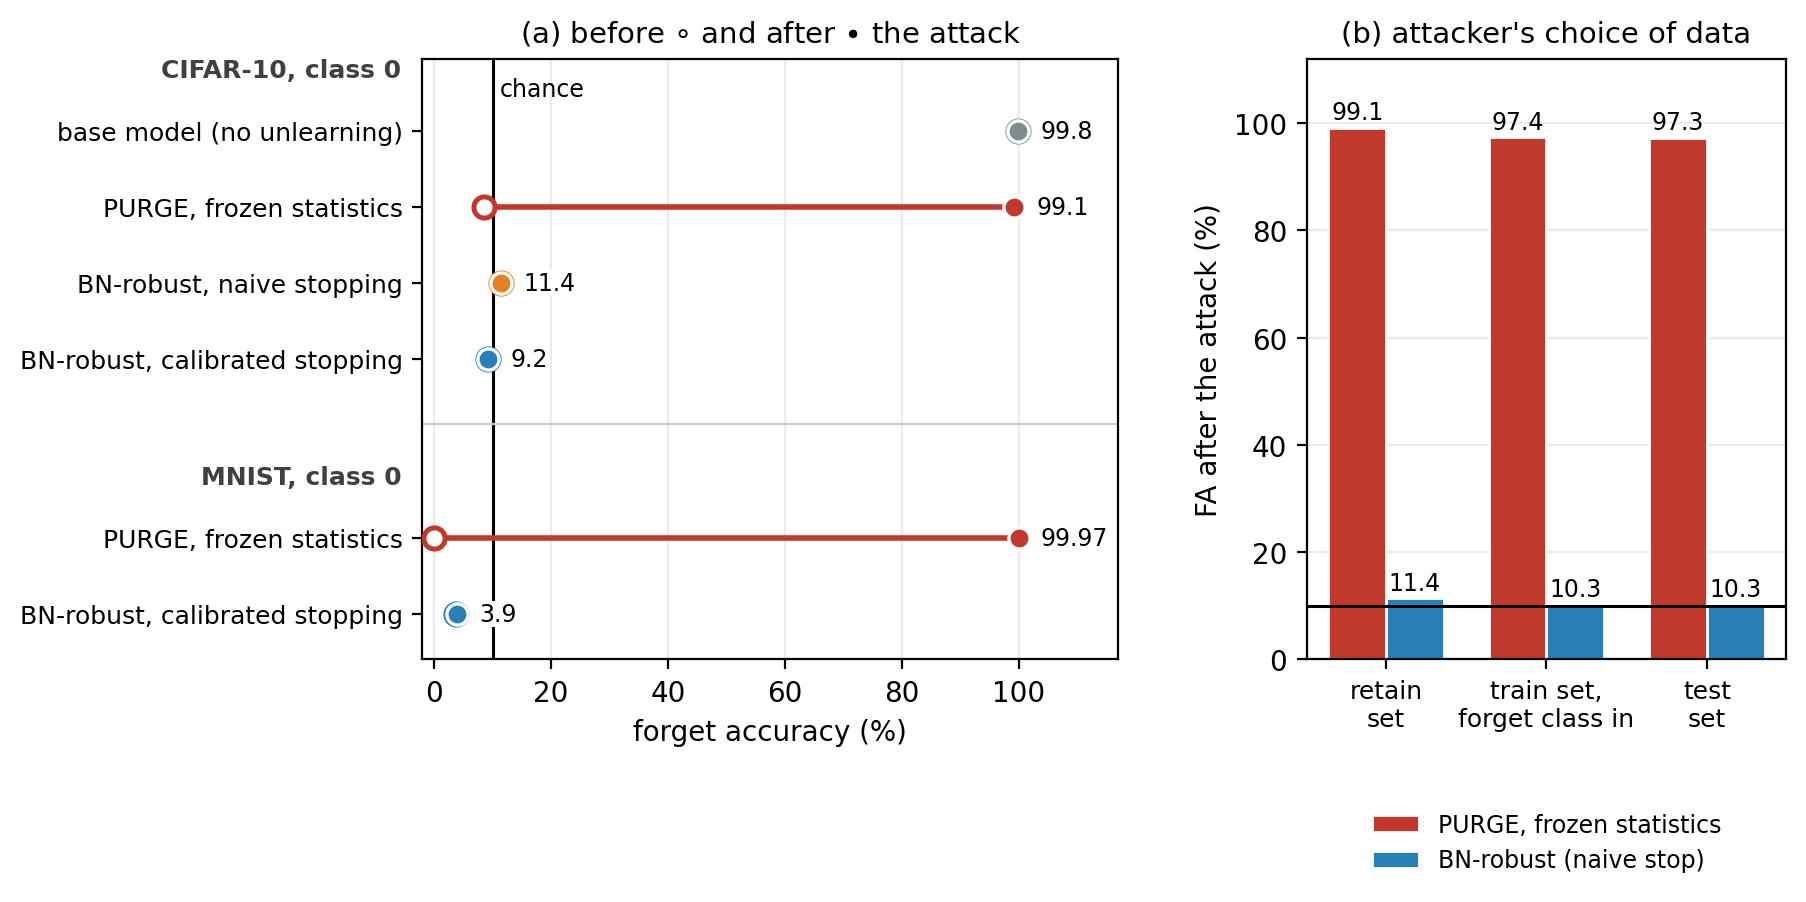
\includegraphics[width=\textwidth]{fig_bnrobust_attack.png}
\caption{\added{\textbf{BN-robust survives the recalibration attack.} (a)~Forget
accuracy before (open) and after (filled) \texttt{update\_bn} on the retain set,
class~0, means over three seeds; on MNIST the frozen configuration's forgetting
is undone completely. (b)~Forget accuracy after the attack when the attacker
recalibrates on the retain set, the full training set (forget class included),
or the test set (CIFAR-10 class~0, three seeds; BN-robust with naive stopping).}}
\label{fig:bnrobust_attack}
\end{figure}

\subsection{Membership Inference Needs a Retrained Reference}\label{sec:mia_main}

\rev{MIA is usually read against $0.5$: an attacker should not be able to tell
forget-class training samples from forget-class test samples. We test that
target against models retrained without the forget class, which trained on
neither group (Table~\ref{tab:mia_main}; Appendix~\ref{sec:mia} adds three
attacks). On CIFAR-10 the reference scores $0.694$ on the loss attack, with a
true-positive rate of $12.5\%$ at $1\%$ false positives, while the base model,
which memorised every member, scores $0.483$: the attack reads a difference in
difficulty between the train and test splits, not membership. Across four
PathMNIST classes the reference ranges from $0.306$ to $0.704$, so no single
constant is the right target. Read against $0.5$, \ours{} looks the worst of the
four methods on CIFAR-10 and SalUn the best; read against the reference, the
order reverses. SalUn's $0.500$ is also degenerate: its true-positive rate is
zero at every threshold, the signature of a constant score. On three of the four
PathMNIST classes \ours{} sits far from its own reference (mean gap
$0.22$--$0.36$ over four attacks), so we claim the protocol finding, not that
\ours{} matches retrained models in general.}

\begin{table}[t]
\centering\color{revisedB}
\caption{\rev{\textbf{Loss-attack MIA against a retrained reference}
(CIFAR-10, class~0). Members are the $5000$ forget-class training images,
non-members the $1000$ forget-class test images; TPR is at $1\%$ FPR.
Appendix~\ref{sec:mia} gives three further attacks and four PathMNIST classes.}}
\label{tab:mia_main}
\small
\begin{tabular}{@{}lccccc@{}}
\toprule
Model & FA & AUROC & TPR & $|\mathrm{AUROC}-0.5|$ & $|\mathrm{AUROC}-\mathrm{ref}|$ \\
\midrule
Retrained (reference) & $0.0$   & $0.694$ & $12.5\%$ & $0.194$ & ---   \\
Base (no unlearning)  & $100.0$ & $0.483$ & $0.0\%$  & $0.017$ & $0.211$ \\
\midrule
SalUn                 & $0.0$   & $0.500$ & $0.0\%$  & $\mathbf{0.000}$ & $0.194$ \\
Bad Teacher           & $24.8$  & $0.485$ & $0.2\%$  & $0.015$ & $0.209$ \\
SCRUB                 & $89.5$  & $0.477$ & $0.4\%$  & $0.023$ & $0.217$ \\
\ours{}               & $2.0$   & $0.693$ & $1.4\%$  & $0.193$ & $\mathbf{0.001}$ \\
\bottomrule
\end{tabular}
\end{table}

\subsection{Further Analyses}\label{sec:further}

The appendices report the remaining experiments in full. \emph{Transformer:} on
ViT-B/16 forgetting transfers \rev{on CIFAR-10}, with FA $9.71\%$ and RA
$97.55\%$, \rev{but not on CIFAR-100 within its 20-epoch cap, where FA ends
between $4.0\%$ and $82.0\%$ across nine classes against a $1\%$ chance level}
(Appendix~\ref{sec:vit}). \emph{Tolerances:} the retain budget is non-binding,
and the forget target is a usable knob over a $29$pp range once it is checked at
every step (Appendix~\ref{sec:sweeps}). \emph{Distance to a retrained model:}
\ours{} is closest in feature space (Fr\'echet distance $13$ against
$153$--$495$ for the baselines) and SalUn in output space
(Appendix~\ref{sec:distance}). \emph{Stopping point:} divergence to a retrained
model is U-shaped along the trajectory with its minimum above chance, and MIA
passes through $0.5$ rather than converging to it
(Appendices~\ref{sec:overforget} and~\ref{sec:trajectory}). \rev{\emph{Sequential
unlearning:} over three classes TA falls from $86.1\%$ to $69.1\%$ and RA from
$100\%$ to $80.7\%$, no more than the forgotten classes themselves account for
(\S\ref{sec:limitations}).}

% ============================================================
\section{Limitations}\label{sec:limitations}

The compute a dataset needs cannot be predicted in advance: the binding resource
is optimiser steps, and STL-10 and CIFAR-100 needed 60 epochs rather than 15 and
20\rev{; ViT-B/16 on CIFAR-100 does not reach chance within its 20-epoch cap}.
Sample-level forgetting works only crudely, because the retain-confusion
target degenerates to uniform when every class remains in the retain set. The
guarantee bounds the sampled mini-batch retain objective, not the population
loss, and holds to float32 precision\rev{; under BN-robust \ours{} it holds per
step under that step's statistics and does not cover the recalibration between
steps}. Our separation from soft conflict-resolution methods
\citep{patel2025learning} is structural; we have not run that method on our
stack. BN-robust \ours{} costs about seven times the compute, was evaluated on
two datasets, and defends only the normalisation statistics, not weight-level
attacks such as fine-tuning recovery\rev{; its comparison with prior methods
rests on the evaluations of \citet{kalani2026batchnorm} and on our own
reproductions, and a like-for-like run of those methods under the same base and
attack remains to be done. In sequential unlearning the retained classes are not
damaged cumulatively, but earlier-forgotten classes partly return: after three
classes RA is $80.7\%$, above the $77.8\%$ that fully forgotten classes would
allow, so they average at least $13\%$ training accuracy, above chance.} \ours{}
gives no differential-privacy guarantee. Appendix~\ref{app:limitations}
discusses each point.

% ============================================================
\section{Conclusion}\label{sec:conclusion}

Unlearning is the dual of continual learning, and \rev{one of continual
learning's most direct tools, a hard constraint on the update, carries over}.
For that constraint to mean anything it must be stated for the update the
optimiser applies: projecting the post-momentum update makes
Theorem~\ref{thm:retain_safety} exact for the deployed optimiser, while the
analysis-friendly alternative \rev{leaves forget accuracy far above chance on
five of six datasets}. Across six datasets and 31 forgetting tasks \ours{}
reaches the chance level on all six (two at a longer budget) with retain
accuracy at or above $97.2\%$ on the 10-class datasets, and \rev{step-level logs
of a CIFAR-10 run} confirm the constraint at every step.
\added{On BatchNorm backbones, keeping the normalisation statistics consistent
with the weights throughout unlearning makes that forgetting survive
recalibration, on every CIFAR-10 class and on MNIST.} The duality is also a
design space: \rev{many continual-learning techniques that protect old-task
knowledge suggest unlearning counterparts} that protect retained knowledge
during erasure. More broadly, when an
optimiser detail is chosen for analytical convenience, it should be checked
against the behaviour it was meant to explain.

\FloatBarrier
% tmlr.bst when available; plainnat keeps the document compilable without it.
\IfFileExists{tmlr.bst}{\bibliographystyle{tmlr}}{\bibliographystyle{plainnat}}
\bibliography{../references}

% ============================================================
\appendix
% ============================================================
\section{Related Work and Positioning in Full}\label{app:related}\label{sec:related_intro}

Approximate unlearning methods occupy different points on the privacy--utility
frontier, and the retain side is where they differ most. \textbf{Gradient
ascent} \citep{thudi2022unrolling} maximises forget-set loss with no mechanism
protecting retain accuracy \rev{(Theorem~\ref{thm:separation}(i))}. \textbf{SalUn} \citep{fan2024salun} confines random-label updates to a
saliency mask---effective in practice, but with no formal retain guarantee and
no control over how much is forgotten. \textbf{SCRUB}
\citep{kurmanji2023unbounded} alternates forget and retain steps balanced by a
weight $\lambda$, so the balance is tuned rather than enforced; in our
reproduction it preserves retain accuracy ($97.7\%$) by barely forgetting at all
(forget accuracy $88.8\%$, Table~\ref{tab:cifar10}). \textbf{NegGrad+}
\citep{thudi2022unrolling} adds a retain-loss term as a weighted sum, again
without a guarantee that retain loss is controlled. Closest to us,
\citet{patel2025learning} diagnose the same forget--retain gradient conflict but
resolve it with a soft regulariser that rewards positive alignment. A fuller treatment, including exact unlearning and distillation-based methods, follows the table.

The distinction we draw is structural rather than numerical, so
Table~\ref{tab:properties} compares properties of each method's \emph{definition}
---checkable against the published update rule, without relying on our
reimplementation of it. A soft penalty biases the optimiser toward retain-safe
steps but leaves harmful steps feasible: for any finite penalty weight, a
sufficiently large forget-loss reduction still makes a retain-harming step
preferable. A projection removes those steps from the feasible set altogether
(Theorem~\ref{thm:separation}(iv)). The final row is the one we would emphasise,
and the one \S\ref{sec:momentum_ablation} makes concrete: a guarantee proved for
a momentum-free surrogate says nothing about a run that uses momentum.

\rev{Figure~\ref{fig:teaser}} places the method against the alternatives on both
what it achieves and what it guarantees.

\paragraph{Exact unlearning.}
SISA \citep{bourtoule2021sisa} partitions data into shards so that removal
requires retraining only the affected shard; the per-deletion cost approaches
full retraining as shard count grows. Certified removal
\citep{guo2020certified} gives exact guarantees for convex models but does not
extend to deep networks.

\paragraph{Gradient-based approximate unlearning.}
GA \citep{thudi2022unrolling} maximises forget-set loss, with no mechanism to
prevent the same direction from degrading retain performance. Amnesiac
unlearning \citep{graves2021amnesiac} subtracts cached per-sample updates,
requiring $O(T|\Df|)$ storage. NegGrad+ optimises
$-\lossf + \lambda\lossr$ directly, which is the Lagrangian relaxation of
Eq.~\ref{eq:problem} rather than a solution to it: the retain term shifts the
optimum without bounding any single step, so the weighted sum is exactly the
soft treatment Theorem~\ref{thm:separation}(iv) separates us from.

\paragraph{Saliency and Fisher methods.}
SalUn \citep{fan2024salun} applies random-label updates inside a top-50\%
saliency mask: strong empirically (FA~$=0\%$ on CIFAR-10) but with no formal
retain guarantee and no control over the degree of forgetting. Fisher-based
methods \citep{golatkar2020eternal,golatkar2021scrubbing} and SSD
\citep{foster2024ssd} weight parameters by estimated importance, requiring
Hessian approximations that scale poorly.

\paragraph{Knowledge distillation.}
Bad Teacher \citep{chundawat2023badteacher} uses competent/incompetent teachers.
SCRUB \citep{kurmanji2023unbounded} is closest in motivation---both draw on CL
intuitions and use KD to anchor retain behaviour---but differs algorithmically:
SCRUB alternates forget and retain steps balanced by $\lambda$, so its balance is
hyperparameter-dependent, whereas \ours{}'s retain safety holds by construction
(Theorem~\ref{thm:separation}); and SCRUB ascends the forget loss, which is
unstable in either direction, whereas \klr{} converges to a specific target
distribution.

\paragraph{Continual learning connection, and the closest prior work.}
A-GEM \citep{chaudhry2019agem} projects task gradients to avoid catastrophic
forgetting. The CL--MU duality has been noted conceptually
\citep{nguyen2020variational,kurmanji2023unbounded}. Closest to \ours{}, recent
work \citep{patel2025learning} also targets the forget--retain gradient
conflict, but through an \emph{implicit, soft} regulariser encouraging a positive
inner product---with no per-step constraint and no formal guarantee. More
broadly, gradient projection and conflict resolution are now actively explored
for unlearning. \added{Closest in mechanism is Projected-Gradient Unlearning
\citep{hoang2024learn}, which takes unlearning steps orthogonal to a gradient
subspace estimated for the retained data. \ours{} differs in the constraint and in
what it binds: a half-space against the current retain gradient---the minimum
correction that excludes retain-harming steps---applied to the post-momentum
update the optimiser actually takes.} \ours{} enforces $\langle u_t,\gr\rangle \ge 0$ explicitly at every
step, on the post-momentum update, which is the difference between \emph{softly
discouraging} conflict and \emph{provably eliminating} it---and, relative to
guarantees stated for momentum-free surrogates, the difference between a bound
that describes the deployed optimiser and one that does not.
\S\ref{sec:strength} tests the mechanism this distinction rests on by varying
our own projection between a soft penalty and the hard constraint; a
like-for-like run of that method on our stack remains future work.

% ============================================================
\section{Design Details}\label{app:method}

\subsection{From the Optimisation Problem to the Algorithm}

This framing makes three things explicit that weighted multi-objective
approaches conflate. First, retain safety is a \emph{hard constraint}, not a
soft penalty. Second, \rev{the forget objective sets the direction of the
search and the forget-accuracy target its end point; only the second is a
constraint}. Third, the two tolerances \rev{$(\alpha, \tau_F)$} are quantities a
practitioner sets, not epochs to be tuned.

\paragraph{Why this needs a new algorithm.} Writing down
Eq.~\ref{eq:problem} is not by itself progress: one could hand it to a generic
constrained solver, or relax it into the weighted objective that existing
methods already optimise. Both routes lose the property we are after. A
Lagrangian relaxation replaces the retain constraint with a penalty
$\lambda\,\lossr$, which is precisely the soft treatment whose feasible set still
contains retain-harming steps (Theorem~\ref{thm:separation}(iv)); and a
projected-gradient solver applied naively would enforce feasibility on the
gradient while the optimiser applies something else
(Proposition~\ref{prop:counter}). What the problem \emph{does} buy is a
specification: it says exactly which quantity each mechanism must control.
\rev{\ours{} realises each condition with the cheapest mechanism we know that
enforces it, and enforces retain safety at every step on the vector actually
applied.} Table~\ref{tab:constraint_map} states that correspondence, and
\S\ref{sec:method} derives each row.

\begin{table}[t]
\centering
\caption{\rev{\textbf{From the problem to the algorithm.} Each condition of
Eq.~\ref{eq:problem}, and the property of the search path, with the mechanism
that enforces it. Two components serve no condition directly: the distillation
anchor, which is part of the retain objective the projection protects, and the
handling of BatchNorm statistics (\S\ref{sec:bn}).}}
\label{tab:constraint_map}
\color{revisedB}
\begin{tabular}{@{}p{0.31\textwidth}p{0.33\textwidth}p{0.28\textwidth}@{}}
\toprule
\textbf{Condition} & \textbf{Mechanism} & \textbf{Enforced} \\
\midrule
Retain objective does not increase along the path &
Projection of the post-momentum update onto $\{\langle u,\gr\rangle \ge 0\}$ (\S\ref{sec:projection}--\ref{sec:optimiser}) &
Every step, to first order on the sampled batch (Thm.~\ref{thm:retain_safety}) \\
\addlinespace
$\CE(\theta;\Dr) \le \alpha\,\CE(\theta_0;\Dr)$ &
Retain-loss stopping rule (\S\ref{sec:stopping}) &
After every epoch, on the full retain set \\
\addlinespace
$\mathrm{FA}(\theta;\Df) \le \tau_F$ &
Forget-accuracy stopping rule (\S\ref{sec:stopping}) &
Every $m$ steps \\
\addlinespace
Direction of the search &
\klr{}: descend $\KL(p_\theta(x_f)\|p_r)$ (\S\ref{sec:forget_obj}) &
Every step \\
\addlinespace
$\|\theta - \theta_0\| \le R$ &
Clipping before accumulation, and the step budget &
$\|\theta_N - \theta_0\| \le N\eta c/(1-\mu)$ \\
\bottomrule
\end{tabular}
\end{table}

\subsection{What Is Taken from A-GEM, and What Is Not}

The operator in
Eq.~\ref{eq:projection} is A-GEM's, and we claim no novelty for it: the
correction $v \mapsto v - \frac{\langle v,g\rangle}{\|g\|^2}g$ is the standard
projection onto a half-space, and \citet{chaudhry2019agem} introduced its use in
continual learning with $g$ the gradient on an episodic memory of past tasks. We
also inherit its two attractive properties: it is the \emph{minimum-norm}
correction restoring feasibility, so it is the least destructive repair of a
conflicting step, and it costs one extra backward pass and one inner product per
step.

What is new is what the operator is asked to do. In A-GEM the projection is a
safeguard on a process whose objective already points the right way---the new
task is being learned, and the memory gradient only occasionally interferes; in
our runs the conflict is not occasional but universal, firing at $100\%$ of
steps (\S\ref{sec:alignment}), because erasing a class and preserving the rest
are directly opposed rather than incidentally so. The projection is therefore
not a correction applied to an optimiser but the optimiser's defining step. That
change of role has three consequences, and they are what
\S\ref{sec:optimiser} is about:
\begin{enumerate}
\item \emph{It must bind the applied vector.} A-GEM projects a gradient; with
momentum the applied vector is not the gradient, and projecting the gradient
certifies nothing (Proposition~\ref{prop:counter}).
\item \emph{Its magnitude matters.} A-GEM tolerates $\|\Pi_{\gr}(v)\| \le \|v\|$
because progress on the new task comes mostly from unconflicted steps. When
every step conflicts, that contraction compounds and forgetting stalls, so we
restore the norm after projecting.
\item \emph{It bounds nothing on the forget side.} The projection guarantees
retain safety and only that; on its own it does not unlearn. Our projection-only
ablation reaches forget accuracy $18.66\%$ against a $10\%$ chance level
(Table~\ref{tab:cifar10}), which is why \ours{} pairs it with a forget objective
rather than presenting the projection as a method.
\end{enumerate}

\subsection{The Three Ordering Choices}

\ours{} uses SGD with momentum $\mu$, weight decay $\lambda_{\mathrm{wd}}$, and
gradient clipping $c$. Three ordering choices determine whether the guarantee is
real, and all three matter empirically.

\paragraph{(i) Project the update, not the gradient.}
The vector applied to the weights is $u_t$, not $\gf$. We therefore
momentum-accumulate first and project afterwards
(Algorithm~\ref{alg:excise}, lines 10--15), so that
$\langle u_t,\gr\rangle \ge 0$ holds for the update that is actually applied.
Projecting $\gf$ instead leaves $\langle u_t,\gr\rangle$ unconstrained.

\paragraph{(ii) Clip before accumulating.}
Clipping is applied to the per-step ingredient $d_t$ \emph{before} it enters the
momentum buffer. This preserves the standard SGD semantics in which momentum
accumulates clipped gradients, and yields the bound
$\|v_t\| \le c/(1-\mu)$ used in Theorem~\ref{thm:retain_safety}. Clipping the
final update instead would cap $\|u_t\| \le c$, destroying the
$1/(1-\mu)$ amplification that momentum provides; since raw forget gradients are
${\sim}100\times$ the clip threshold in our runs, clipping is always active, and
this ordering is the difference between forgetting and not forgetting.

\paragraph{(iii) Preserve magnitude under projection.}
Projection is norm-non-increasing: $\|\Pi_{\gr}(v)\| = \|v\|\sin\vartheta$ where
$\vartheta$ is the angle between $v$ and $\gr$. When forget and retain gradients
are nearly antiparallel, $\sin\vartheta \approx 0$ and the applied step
collapses, stalling forgetting for reasons unrelated to retain safety. We
therefore rescale the projected update to the pre-projection norm,
$u_t = \Pi_{\gr}(v_t)\,\|v_t\|/\|\Pi_{\gr}(v_t)\|$. Because
$\langle u,\gr\rangle = 0$ is invariant to positive rescaling, this leaves the
guarantee untouched while decoupling forgetting speed from conflict severity.
(If $\Pi_{\gr}(v_t)=0$, i.e.\ $v_t$ is exactly antiparallel to $\gr$, we set
$u_t=0$; the guarantee holds trivially.)

\subsection{The Forget Objective}

The \klr{} objective of Eq.~\ref{eq:kl_retain} targets $p_r$,
where $p_r$ (Eq.~\ref{eq:retain_confuse}) is the model's natural confusion
pattern. The motivation is that no trained model produces uniform outputs, so a
model driven toward $\mathcal{U}(K)$ remains separable from a retrained one even
at FA~$=0\%$; a forget target drawn from the model's own behaviour on retained
data does not have that artefact. Under the previous implementation this was
supported empirically, with the uniform target giving MIA AUROC~$=0.469$ against
$0.496$ for \klr{}. \textbf{Re-measured under the projected-momentum optimiser,
it is not.} The three forget objectives give, on CIFAR-10 class~0:
gradient ascent $\mathrm{TA}/\mathrm{FA}/\mathrm{MIA} = 86.4/8.2/0.559$,
KL-uniform $86.4/3.9/0.526$, and \klr{} $86.1/2.1/0.528$. Both KL variants
clearly beat gradient ascent, which neither forgets as far nor stays as close to
the ideal MIA. Between the two, however, the difference is within noise and if
anything favours uniform ($|\mathrm{MIA}-0.5| = 0.026$ against $0.028$).

We therefore keep \klr{} for its lower forget accuracy at equal test accuracy,
and retract the claim that it is distinguishable from the uniform target on
MIA grounds. This is consistent with \S\ref{sec:overforget}: $p_r$ is not what a
retrained model produces on forget inputs, so an argument resting on $p_r$ being
the ``natural'' target was never on firm ground. What survives is narrower---%
$p_r$ is a better forget \emph{direction} than uniform, and no more. It is not a claim that $p_r$ is what a retrained model
outputs on forget inputs: \S\ref{sec:overforget} and
Appendix~\ref{app:d2r} show it is not, and that minimising the divergence to it
is harmful.

\subsection{Supporting Components}

\paragraph{KD-anchored stability.}
A frozen copy of $\theta_0$ serves as teacher,
$\losskd = T^2\KL(\sigma(f_\theta(x_r)/T)\|\sigma(f_{\theta_0}(x_r)/T))$,
anchoring behaviour on $\Dr$ and complementing the projection.

\section{Notation, Assumptions, and the Analysed Update}\label{app:setup}

We restate the update exactly as implemented, since the entire point of
Theorem~\ref{thm:retain_safety} is that the analysed object and the executed
object coincide.

\paragraph{Notation.}
\rev{$\Lrt(\theta)$ is the retain objective $\lossr$ of
\S\ref{sec:problem}---cross-entropy plus $\beta\losskd(\theta,\theta_0;\Dr)$---}%
evaluated on the sampled retain mini-batch at step $t$, and $\gr := \nabla_\theta\Lrt(\theta_t)$ its gradient. Note $\beta$ does not
appear separately in the bounds because $\gr$ is already the composite gradient.
$\gf := \nabla_\theta\lossf(\theta_t;x_f)$ is the forget gradient on the forget
mini-batch. $\lambda_{\mathrm{wd}} \ge 0$ is weight decay, $c>0$ the clipping
threshold, $\eta>0$ the learning rate, and $\mu\in[0,1)$ the momentum
coefficient. $\|\cdot\|$ is the Euclidean norm on the concatenation of all
trainable parameters.

\paragraph{The projection operator.}
For $g \ne 0$ define
\begin{equation}\label{eq:app_proj}
\Pi_{g}(v) \;=\;
\begin{cases}
v, & \langle v,g\rangle \ge 0,\\[2pt]
v - \dfrac{\langle v,g\rangle}{\|g\|^{2}}\,g, & \langle v,g\rangle < 0,
\end{cases}
\qquad
\widehat{\Pi}_{g}(v) \;=\;
\begin{cases}
\Pi_g(v)\,\dfrac{\|v\|}{\|\Pi_g(v)\|}, & \Pi_g(v) \ne 0,\\[4pt]
0, & \Pi_g(v) = 0,
\end{cases}
\end{equation}
where $\widehat{\Pi}$ is the \emph{magnitude-preserving} variant used by \ours{}
(\S\ref{sec:optimiser}). In the implementation the case $\Pi_g(v)=0$ is detected
by the guard $\|\Pi_g(v)\| \le \epsilon\|v\|$ with $\epsilon = 10^{-8}$.

\paragraph{The analysed (and executed) update.}
With $v_{-1}=0$, for $t = 0,1,2,\dots$
\begin{align}
d_t &= \mathrm{clip}_c\!\big(\gf^{(t)} + \lambda_{\mathrm{wd}}\theta_t\big),
      &&\text{where } \mathrm{clip}_c(x) = x\cdot\min\!\big(1, c/\|x\|\big),
      \label{eq:app_clip}\\
v_t &= \mu\,v_{t-1} + d_t, \label{eq:app_mom}\\
u_t &= \widehat{\Pi}_{\gr^{(t)}}(v_t), \label{eq:app_projstep}\\
\theta_{t+1} &= \theta_t - \eta\,u_t. \label{eq:app_step}
\end{align}
Three orderings are load-bearing and are stated here so they cannot be lost in
implementation: clipping acts on $d_t$ \emph{before} the momentum accumulation
(\ref{eq:app_clip})--(\ref{eq:app_mom}); the projection acts on the accumulated
$v_t$, i.e.\ on the update rather than on the gradient (\ref{eq:app_projstep});
and no clipping is applied after (\ref{eq:app_projstep}).

\paragraph{Assumptions.}
\begin{itemize}
\item[(A1)] $\Lrt$ is $L$-smooth: $\|\nabla\Lrt(x)-\nabla\Lrt(y)\| \le L\|x-y\|$
for all $x,y$.
\item[(A2)] Clipping is applied as in (\ref{eq:app_clip}), so $\|d_t\| \le c$ for
all $t$.
\item[(A3)] $\mu \in [0,1)$.
\end{itemize}
(A1) is the standard smoothness assumption of first-order analysis; for ReLU
networks it holds piecewise, and we treat it as an idealisation, as is
conventional. (A2) and (A3) are properties of the implementation, not
assumptions about the data.

% ------------------------------------------------------------
\section{Proof of Theorem~\ref{thm:retain_safety}}\label{app:thm1}

We prove three lemmas and then assemble the theorem.

\begin{lemma}[Projection properties]\label{lem:proj}
Let $g \ne 0$ and $v$ be arbitrary. Then
\begin{enumerate}
\item[(i)] $\langle \Pi_g(v), g\rangle \ge 0$, with equality whenever
$\langle v,g\rangle < 0$;
\item[(ii)] $\|\Pi_g(v)\| \le \|v\|$;
\item[(iii)] $\langle \widehat{\Pi}_g(v), g\rangle \ge 0$ and
$\|\widehat{\Pi}_g(v)\| \le \|v\|$, with $\|\widehat{\Pi}_g(v)\| = \|v\|$
whenever $\Pi_g(v)\ne 0$.
\end{enumerate}
\end{lemma}

\begin{proof}
(i) If $\langle v,g\rangle \ge 0$ then $\Pi_g(v)=v$ and the claim is immediate.
If $\langle v,g\rangle<0$ then
\[
\langle \Pi_g(v), g\rangle
= \Big\langle v - \tfrac{\langle v,g\rangle}{\|g\|^2}g,\; g\Big\rangle
= \langle v,g\rangle - \tfrac{\langle v,g\rangle}{\|g\|^2}\|g\|^2 = 0 .
\]
(ii) In the first branch this is an equality. In the second branch, $\Pi_g$ is
the orthogonal projection onto the hyperplane $\{u:\langle u,g\rangle=0\}$;
writing $v = \Pi_g(v) + \tfrac{\langle v,g\rangle}{\|g\|^2}g$ as a sum of two
orthogonal vectors, Pythagoras gives
\begin{equation}\label{eq:app_pyth}
\|v\|^2 = \|\Pi_g(v)\|^2 + \frac{\langle v,g\rangle^2}{\|g\|^2}
\;\ge\; \|\Pi_g(v)\|^2 .
\end{equation}
(iii) If $\Pi_g(v)=0$ then $\widehat{\Pi}_g(v)=0$ and both claims are trivial.
Otherwise $\widehat{\Pi}_g(v) = s\,\Pi_g(v)$ with
$s = \|v\|/\|\Pi_g(v)\| > 0$, so
$\langle \widehat{\Pi}_g(v),g\rangle = s\langle \Pi_g(v),g\rangle \ge 0$ by (i),
and $\|\widehat{\Pi}_g(v)\| = s\|\Pi_g(v)\| = \|v\|$.
\end{proof}

Part (iii) is the formal content of the design choice in
\S\ref{sec:optimiser}(iii): rescaling restores the magnitude that
(\ref{eq:app_pyth}) removes, and because $s>0$ it cannot flip the sign of the
inner product. The guarantee is therefore invariant to the rescaling, while the
step magnitude is not.

\begin{lemma}[Velocity norm bound]\label{lem:vel}
Under (A2) and (A3), for every $t \ge 0$,
\begin{equation}\label{eq:app_velbound}
\|v_t\| \;\le\; c\,\frac{1-\mu^{\,t+1}}{1-\mu} \;<\; \frac{c}{1-\mu}.
\end{equation}
\end{lemma}

\begin{proof}
Unrolling (\ref{eq:app_mom}) from $v_{-1}=0$ gives
$v_t = \sum_{k=0}^{t}\mu^{\,t-k} d_k$. By the triangle inequality and (A2),
\[
\|v_t\| \;\le\; \sum_{k=0}^{t}\mu^{\,t-k}\|d_k\|
\;\le\; c\sum_{j=0}^{t}\mu^{\,j}
\;=\; c\,\frac{1-\mu^{\,t+1}}{1-\mu}
\;<\; \frac{c}{1-\mu},
\]
the last step using $\mu\in[0,1)$ so that $\mu^{t+1}>0$ and the geometric series
converges.
\end{proof}

Lemma~\ref{lem:vel} is where the clip-before-momentum ordering is used: it
requires $\|d_k\|\le c$ for the \emph{ingredients} of the sum. Note also that the
bound is attained only in the limit of perfectly aligned successive steps; we
observe $\max_t\|u_t\| = 9.16$ against $c/(1-\mu)=10$ in
\S\ref{sec:alignment}, so it is tight in practice.

\begin{lemma}[Descent step]\label{lem:descent}
Under (A1), for any vector $u$ and $\theta_{+} = \theta_t - \eta u$,
\begin{equation}\label{eq:app_descent}
\Lrt(\theta_{+}) \;\le\; \Lrt(\theta_t) - \eta\langle u, \gr\rangle
+ \tfrac{1}{2}L\eta^2\|u\|^2 .
\end{equation}
\end{lemma}

\begin{proof}
Standard consequence of $L$-smoothness (the descent lemma): (A1) implies
$\Lrt(y) \le \Lrt(x) + \langle \nabla\Lrt(x), y-x\rangle + \tfrac{L}{2}\|y-x\|^2$
for all $x,y$. Substituting $x=\theta_t$, $y=\theta_+$, so that
$y-x = -\eta u$ and $\nabla\Lrt(x)=\gr$, gives (\ref{eq:app_descent}).
\end{proof}

\begin{theorem}[Theorem~\ref{thm:retain_safety}, restated]\label{thm:app_main}
Under (A1)--(A3), the update (\ref{eq:app_clip})--(\ref{eq:app_step}) satisfies,
at every step $t$ and unconditionally,
\begin{align}
\text{(a)}\quad & \langle u_t, \gr^{(t)}\rangle \;\ge\; 0, \label{eq:app_a}\\
\text{(b)}\quad & \|u_t\| \;\le\; \|v_t\| \;<\; \frac{c}{1-\mu},
   \quad\text{with }\|u_t\|=\|v_t\|\text{ unless }\Pi_{\gr}(v_t)=0,
   \label{eq:app_b}\\
\text{(c)}\quad & \Lrt(\theta_{t+1}) \;\le\; \Lrt(\theta_t)
   + \tfrac{1}{2}L\eta^{2}\Big(\frac{c}{1-\mu}\Big)^{\!2}. \label{eq:app_c}
\end{align}
\end{theorem}

\begin{proof}
(a) Immediate from Lemma~\ref{lem:proj}(iii) applied to $v_t$ with
$g=\gr^{(t)}$, using (\ref{eq:app_projstep}). If $\gr^{(t)}=0$ the projection is
undefined and is skipped; then $\langle u_t,\gr^{(t)}\rangle = 0$ and (a) holds
trivially (see Remark~\ref{rem:degenerate}).

(b) Combine Lemma~\ref{lem:proj}(iii) with Lemma~\ref{lem:vel}.

(c) By Lemma~\ref{lem:descent} with $u = u_t$,
\[
\Lrt(\theta_{t+1}) \le \Lrt(\theta_t) - \eta\underbrace{\langle u_t,\gr^{(t)}\rangle}_{\ge\,0\ \text{by (a)}}
+ \tfrac{1}{2}L\eta^2\underbrace{\|u_t\|^2}_{<\,(c/(1-\mu))^2\ \text{by (b)}}
\;\le\; \Lrt(\theta_t) + \tfrac{1}{2}L\eta^2\Big(\frac{c}{1-\mu}\Big)^{\!2}. \qedhere
\]
\end{proof}

The first-order change in the sampled retain objective is thus non-positive at
every step; the only admissible increase is the $O(\eta^2)$ curvature term. The
guarantee is \emph{unconditional} in the sense that it requires no assumption on
$\gf$, on the alignment between forget and retain gradients, or on the data.

\begin{corollary}[Momentum-free reduction]\label{cor:mu0}
Setting $\mu=0$ gives $v_t = d_t$, $\|u_t\|\le c$, and
$\Lrt(\theta_{t+1}) \le \Lrt(\theta_t) + \tfrac{1}{2}L\eta^2c^2$, recovering the
momentum-free per-step bound.
\end{corollary}

\begin{corollary}[A-GEM reduction]\label{cor:agem}
Setting $\mu=0$, $c=\infty$ and letting $\eta\to0$ recovers the first-order
A-GEM guarantee $\langle u_t,\gr\rangle\ge0$ \citep{chaudhry2019agem}.
\end{corollary}

Corollary~\ref{cor:mu0} is worth reading alongside
Table~\ref{tab:momentum}: the $\mu=0$ bound is \emph{formally tighter} (by a
factor $(1-\mu)^{-2}=100$ at $\mu=0.9$), yet the configuration it describes
fails to unlearn on five of six datasets. A tighter bound on a method that does
not forget is not the better result---which is precisely why we analyse the
update that is actually run.

\subsection{Why the Projection Must Be Applied to the Update}\label{app:counterexample}

The following proposition shows that the design choice of
\S\ref{sec:optimiser}(i) is not a matter of convenience: projecting the
\emph{gradient} provides no per-step guarantee once $\mu>0$, however carefully
each individual gradient is projected.

\begin{proposition}[Gradient-projection is insufficient under momentum]\label{prop:counter}
Consider the variant that projects the gradient and then accumulates momentum:
\[
\tilde d_t = \mathrm{clip}_c\big(\Pi_{\gr^{(t)}}(\gf^{(t)})\big), \qquad
v_t = \mu v_{t-1} + \tilde d_t, \qquad \theta_{t+1} = \theta_t - \eta v_t ,
\]
so that every accumulated ingredient satisfies
$\langle \tilde d_t, \gr^{(t)}\rangle \ge 0$. Then for every $\mu \in (0,1)$
there exist retain and forget gradients for which the applied update $v_t$
satisfies $\langle v_t, \gr^{(t)}\rangle < 0$, i.e.\ the step strictly increases
the sampled retain loss to first order.
\end{proposition}

\begin{proof}
Work in $\mathbb{R}^2$ with $\lambda_{\mathrm{wd}}=0$, $c=\infty$ (clipping
inactive), and $v_{-1}=0$.

\emph{Step $0$.} Let $\gr^{(0)} = (1,0)$ and $\gf^{(0)} = (-1,1)$. Then
$\langle \gf^{(0)},\gr^{(0)}\rangle = -1 < 0$, so the projection fires:
\[
\tilde d_0 = \Pi_{\gr^{(0)}}(\gf^{(0)})
= (-1,1) - \frac{-1}{1}(1,0) = (0,1),
\]
which is retain-safe, $\langle \tilde d_0, \gr^{(0)}\rangle = 0$. Hence
$v_0 = (0,1)$.

\emph{Step $1$.} Let the retain mini-batch change so that
$\gr^{(1)} = (0,-1)$, and let $\gf^{(1)} = (1,0)$. Then
$\langle \gf^{(1)},\gr^{(1)}\rangle = 0 \ge 0$, so no projection is needed and
$\tilde d_1 = (1,0)$, again retain-safe:
$\langle \tilde d_1,\gr^{(1)}\rangle = 0$. The applied update is
\[
v_1 = \mu v_0 + \tilde d_1 = \mu(0,1) + (1,0) = (1,\mu),
\qquad
\langle v_1, \gr^{(1)}\rangle = \langle (1,\mu), (0,-1)\rangle = -\mu \;<\; 0
\]
for every $\mu>0$. By Lemma~\ref{lem:descent} the first-order change in $\Lrt$
is $-\eta\langle v_1,\gr^{(1)}\rangle = +\eta\mu > 0$: the retain loss strictly
increases to first order, even though \emph{every} projected gradient entering
the buffer was individually retain-safe.
\end{proof}

The mechanism is transparent: the momentum buffer carries a direction that was
certified against $\gr^{(0)}$ into a step whose constraint is $\gr^{(1)}$, and
the projection at step $1$ never inspects the carried term. Projecting $v_t$
itself (\ref{eq:app_projstep}) removes exactly this failure, because the
certificate is issued against the constraint in force at the step where the
update is applied. Note also that $\mu$ appears linearly in the violation, so the
defect grows with the momentum coefficient rather than vanishing.

\subsection{Why Clipping Must Precede Accumulation}\label{app:clip_order}

\begin{proposition}[Clipping the update destroys momentum amplification]\label{prop:clip}
Consider the variant that clips the final update,
$u_t = \mathrm{clip}_c(\widehat{\Pi}_{\gr}(\mu v_{t-1} + \tilde g_t))$ with
$\tilde g_t$ unclipped. Then $\|u_t\| \le c$ for all $t$, identical to the bound
obtained at $\mu=0$ (Corollary~\ref{cor:mu0}), irrespective of $\mu$.
\end{proposition}

\begin{proof}
Immediate from the definition of $\mathrm{clip}_c$.
\end{proof}

Proposition~\ref{prop:clip} is trivial as mathematics but decisive in practice.
In our runs the raw forget-gradient norm is ${\sim}100\times$ the clipping
threshold ($\|\gf\| \in [102,149]$ with $c=1$ on CIFAR-10), so clipping is active
at every step and the cap is always attained. Clipping after accumulation
therefore yields an applied step of magnitude exactly $\eta c$ --- the same
magnitude as the momentum-free configuration, and hence the same failure to
forget documented in Table~\ref{tab:momentum}. The ordering in
(\ref{eq:app_clip})--(\ref{eq:app_mom}) instead admits
$\|v_t\| \to c/(1-\mu)$, a $10\times$ larger step at $\mu=0.9$, while
Lemma~\ref{lem:vel} keeps it bounded. The bound in (\ref{eq:app_c}) is looser by
$(1-\mu)^{-2}$ as a result; this is the price of a guarantee that describes an
optimiser that unlearns.

\subsection{Remarks on Scope and Exactness}

\begin{remark}[Mini-batch scope]\label{rem:minibatch}
$\gr^{(t)}$ is the gradient of the retain objective on the \emph{sampled} retain
mini-batch, so (\ref{eq:app_c}) is exact for that mini-batch's objective---which
is the quantity \ours{} projects against, and therefore the quantity about which
a per-step statement can be made. Because mini-batch gradients are unbiased
estimates of the population gradient, the first-order term is non-positive in
expectation up to the standard SGD gradient-variance term; a population-exact
per-step guarantee would require the full retain gradient at every step, at
$O(|\Dr|)$ cost per update. We regard this as the principal formal limitation
(\S\ref{sec:limitations}).
\end{remark}

\begin{remark}[Degenerate retain gradient]\label{rem:degenerate}
The implementation skips the projection when $\|\gr\|^2 < 10^{-12}$, since
(\ref{eq:app_proj}) is then numerically ill-posed. In that regime the violation
of (\ref{eq:app_a}) is bounded by Cauchy--Schwarz:
$|\langle u_t,\gr\rangle| \le \|u_t\|\|\gr\| \le 10^{-6}c/(1-\mu)$, giving a
first-order retain increase of at most $10^{-5}\eta$. Moreover such a $\gr$
means the retain mini-batch is already at a stationary point. The exception is
therefore quantitatively negligible, but we state it rather than suppress it.
\end{remark}

\begin{remark}[Floating-point exactness]\label{rem:float}
In exact arithmetic $\langle \Pi_g(v),g\rangle = 0$ identically. In float32, the
inner products are sums over $1.12\times10^7$ parameters, with accumulation
error of order $\sqrt{n}\,\varepsilon_{32} \approx 4\times10^{-4}$ relative.
The measured worst-case relative violation is $-7.4\times10^{-7}$
(\S\ref{sec:alignment}), three orders of magnitude \emph{below} that scale and
with positive mean, consistent with rounding rather than a systematic defect. We
therefore state Theorem~\ref{thm:app_main} as holding to float32 precision, and
recommend float64 accumulation for the inner products in
(\ref{eq:app_proj}) in reference implementations.
\end{remark}

% ------------------------------------------------------------
\section{Proof of Theorem~\ref{thm:separation}}\label{app:thm2}

\begin{theorem}[Theorem~\ref{thm:separation}, restated]\label{thm:app_sep}
Fix $\theta_0$ with retain gradient $\gr := \nabla\Lrt(\theta_0) \ne 0$ and
forget gradient $\gf$. Consider one-step update operators. Then:
\begin{enumerate}
\item[(i)] \textbf{GA.} The update $\theta_0 + \eta\gf$ strictly increases
$\Lrt$ to first order whenever $\langle \gf,\gr\rangle > 0$.
\item[(ii)] \textbf{SCRUB.} For any fixed $\lambda>0$ there exist $\gf,\gr$ with
$\langle -\gf+\lambda\gr,\;\gr\rangle < 0$.
\item[(iii)] \textbf{SalUn.} The masked random-label update
$-M\odot\nabla\CE_{\mathrm{RL}}$ has unconstrained sign with respect to $\gr$.
\item[(iv)] \textbf{Soft conflict regularisers.} Penalising negative alignment
does not preclude it.
\item[(v)] \textbf{\ours{}.} $\langle u_t,\gr\rangle \ge 0$ unconditionally.
\end{enumerate}
\end{theorem}

\begin{proof}
(i) A first-order expansion gives
$\Lrt(\theta_0+\eta\gf) = \Lrt(\theta_0) + \eta\langle \gf,\gr\rangle + O(\eta^2)$,
which exceeds $\Lrt(\theta_0)$ for small $\eta>0$ when
$\langle\gf,\gr\rangle>0$. Since GA constrains neither the sign nor the
magnitude of $\langle\gf,\gr\rangle$, no configuration-independent per-step
guarantee is available.

(ii) Compute
$\langle -\gf+\lambda\gr,\;\gr\rangle = -\langle\gf,\gr\rangle+\lambda\|\gr\|^2$.
This is negative precisely when
$\langle\gf,\gr\rangle > \lambda\|\gr\|^2$. Such a pair exists for any fixed
$\lambda$: e.g.\ in $\mathbb{R}^2$ take $\gr=(1,0)$ and
$\gf = (\lambda+1)\,(1,0)$, giving
$\langle\gf,\gr\rangle = \lambda+1 > \lambda = \lambda\|\gr\|^2$. Because
$\lambda$ is a fixed hyperparameter while $\langle\gf,\gr\rangle/\|\gr\|^2$
varies along the trajectory, no fixed $\lambda$ certifies every step.

(iii) With random labels the masked gradient direction is uncorrelated with
$\gr$ in expectation; individual draws therefore realise either sign of
$\langle g_{\mathrm{SalUn}},\gr\rangle$, and the mask $M$ (selected by gradient
magnitude, not by retain alignment) imposes no constraint on it.

(iv) A regulariser adding $\rho\,\phi(\langle g,\gr\rangle)$ to the objective
with $\phi$ decreasing shifts the optimum toward positive alignment but leaves
the feasible set unrestricted: for any finite penalty weight $\rho$, a
sufficiently large forget-loss reduction makes a step with
$\langle g,\gr\rangle<0$ preferable. Only a hard constraint---i.e.\ a projection
onto $\{u:\langle u,\gr\rangle\ge0\}$---renders such steps unreachable.

(v) Theorem~\ref{thm:app_main}(a).
\end{proof}

\begin{remark}
Theorem~\ref{thm:app_sep} is a \emph{worst-case} separation: it exhibits
configurations in which the baselines strictly degrade the retain objective in a
single step, not a claim that they typically do. In practice all these methods
often produce small retain-loss changes. The distinction the theorem draws is
between behaviour that is empirically usual and behaviour that is guaranteed by
construction; only the latter is checkable without running the method.
\end{remark}

% ------------------------------------------------------------
% ============================================================
\section{Extended Experimental Results}\label{app:experiments}

\subsection{Datasets, Baselines and Metrics}

We also fix the four quantities used to evaluate unlearning throughout, so that
they are available before the algorithm is stated. \emph{Test accuracy} (TA) is
measured on the held-out test set and reports how much of the model's general
utility survives. \emph{Forget accuracy} (FA) is measured on $\Df$; because a
retrained model has never seen those samples, a fully unlearned model should
drive FA down to at most the chance level $100/K\%$. \emph{Retain accuracy} (RA)
is measured on $\Dr$ and should not move. Finally, a
\emph{membership-inference attack} (MIA) tries to distinguish forget-set
training samples from forget-set test samples, and we score it by the area under
its receiver-operating-characteristic curve (AUROC); this is conventionally read
against an ideal of $0.5$, a convention \S\ref{sec:mia} shows to be the wrong
reference point.

\paragraph{Datasets.}
We evaluate on six image-classification benchmarks chosen to vary the three
factors that plausibly govern how hard class-level unlearning is: the number of
classes, the number of examples per class, and the semantic distance between the
forgotten class and the retained ones.

CIFAR-10 \citep{krizhevsky2009cifar} is the standard unlearning benchmark and
serves as our reference setting. MNIST \citep{lecun1998mnist} and SVHN
\citep{netzer2011svhn} share its ten-class structure but differ in difficulty
and in how strongly classes overlap, which lets us separate the method's
behaviour from the particular geometry of CIFAR-10. CIFAR-100
\citep{krizhevsky2009cifar} raises the class count tenfold, lowering the chance
level to $1\%$ and shrinking each forget set to $500$ images---a regime where
``forgotten'' is a far stricter requirement. STL-10 \citep{coates2011stl10}
isolates data scarcity in the other direction: at $96{\times}96$ resolution with
only $500$ training images per class, the forget set yields roughly $60$
optimiser steps, which stresses any method that must make progress under a
per-step constraint. PathMNIST \citep{yang2023medmnist} moves off natural
images entirely to histopathology tissue types, where class boundaries are less
separable and where deletion requests are a realistic rather than hypothetical
requirement.

Forgetting a single class can be unrepresentative---classes differ substantially
in difficulty---so wherever cost permits we forget \emph{every} class in turn:
all ten for MNIST and all nine for PathMNIST, with per-class results reported in
Appendix~\ref{app:perclass} rather than only in aggregate. For CIFAR-100 we
sample one class per tens group (classes $10$--$90$) to cover the label space at
tractable cost, and for CIFAR-10, SVHN, and STL-10 we forget class~0 across
three seeds to quantify run-to-run variance. This gives 31 forgetting tasks and
75 unlearning runs in total.

\paragraph{Model, baselines, metrics.}
All experiments use ResNet-18 \citep{he2016resnet} (11.7M parameters). We
compare against \rev{a model retrained without the forget class}, SalUn
\citep{fan2024salun}, SCRUB \citep{kurmanji2023unbounded}, Bad Teacher
\citep{chundawat2023badteacher}, and NegGrad+ \citep{thudi2022unrolling}, all
re-run on our stack\rev{; every MIA number except SalUn's in
Table~\ref{tab:cifar10} comes from one attack implementation, the mean AUROC of
a loss and a confidence attack,} rather than being quoted from each method's own
paper. We report
the four metrics defined in \S\ref{sec:problem}: TA, FA, RA, and MIA AUROC. Two
reminders about FA are worth repeating here: the target is the chance level
$100/K\%$ rather than zero, and a retrained reference in fact reaches
${\approx}0\%$ because it routes forget-class inputs to surviving classes.

\paragraph{Hyperparameters.}
CIFAR-10: $\eta=5{\times}10^{-4}$, $\mu=0.9$, $\beta=2.0$, $c=1.0$,
$\alpha=5.0$, $T_{\mathrm{KD}}=4.0$. Other datasets use
$\eta=2{\times}10^{-4}$, $\beta\in[3,5]$. All configs are released as YAML.

\subsection{Cross-Dataset Results in Detail}\label{app:cross}

Table~\ref{tab:cross} reports the main results. At \rev{each dataset's epoch
cap} \ours{} drives FA to or below the chance level on four of six datasets and holds
RA $\ge 97.2\%$ everywhere except CIFAR-100 ($92.2\%$); at the extended budget it
reaches chance on all six. \rev{The mean over seeds is below chance for every
MNIST and PathMNIST class.} The
two shortfalls in the upper block---STL-10 and CIFAR-100---are budget-limited
rather than method-limited, and \S\ref{sec:crossdataset_stl} separates the two
explanations.

The per-dataset mean MIA AUROC stays within $0.035$ of $0.5$ on all six
datasets. We report that because it is the conventional summary, but
\S\ref{sec:mia} shows $0.5$ is not the right reference point for this
protocol---and that no fixed reference point is---so it should not be read as
evidence of successful unlearning on its own.

The MIA figure above is a per-dataset \emph{mean}, and on PathMNIST that mean
conceals a defect: two individual classes sit at $0.298$ and $0.388$, well
\emph{below} $0.5$ rather than above it (Appendix~\ref{app:perclass}). We
report this rather than let the aggregate absorb it, and we return to it in
\S\ref{sec:overforget}.

\paragraph{The two shortfalls are budget-limited, not method-limited.}
\label{sec:crossdataset_stl}
\rev{Table~\ref{tab:cross} sets an epoch cap per dataset (12--20 epochs), which
penalises datasets with few images per class, since the binding resource is
update steps rather than examples. STL-10 supplies only 4 forget mini-batches
per epoch, so its 15-epoch cap buys ${\sim}60$ steps against ${\sim}600$ for
CIFAR-10 at the same cap. Raising STL-10 to 60 epochs, with a per-step check and
a $1\%$ forget target, takes forget accuracy from $75.67\%$ to
$\mathbf{1.73\%}$ over the same three seeds ($1.0$--$2.8\%$), at
RA~$=98.87\%$ and MIA~$=0.488$; a single 60-epoch run with the default $10\%$
target stops at $9.20\%$ after 30 epochs, so reaching chance does not depend on
the tighter target. Test accuracy moves from $92.84\%$ to $85.15\%$}, which
is not collateral damage but the arithmetic of having actually forgotten: TA is
measured over all $K$ classes, so removing one of ten costs a tenth of it, and
$85.15 = 94.61 \times \tfrac{9}{10}$ leaves the retained classes at $94.61\%$.
The same operation on CIFAR-10 gives $86.13 = 95.70 \times \tfrac{9}{10}$, so
under the longer budget STL-10 behaves like the datasets that already worked
rather than like a failure case.

CIFAR-100 responds likewise, and more informatively. Re-running all nine
tens-group classes at 60 epochs takes the mean from $4.07\%$ to
$\mathbf{1.27 \pm \rev{0.39}\%}$ against a $1\%$ chance level---so the chance level now
lies within one standard deviation---while the spread across classes collapses
from $\pm 5.51$ to $\pm \rev{0.39}$. The earlier variance was therefore not an
intrinsic property of the 100-class setting but a symptom of some classes being
halted before convergence: the outlier that failed to converge within $20$
epochs (FA $17.8\%$) reaches $2.0\%$ given $60$. Retain accuracy costs $0.87$pp
for this ($92.19 \to 91.32$).

Both re-runs use the same seeds and classes as the \rev{upper-block rows, with
a per-step check,} so we report them as a second block of Table~\ref{tab:cross}
rather than substituting them into the first. The distinction is worth
preserving: at \rev{the configured caps} the method reaches chance on four of
six datasets, and at a budget scaled to the data it reaches chance on all six.
Which is the honest headline depends on whether a practitioner will spend
\rev{three to four} times the compute on small or many-class datasets, so we
report both and label them.

\begin{figure}[t]
\centering
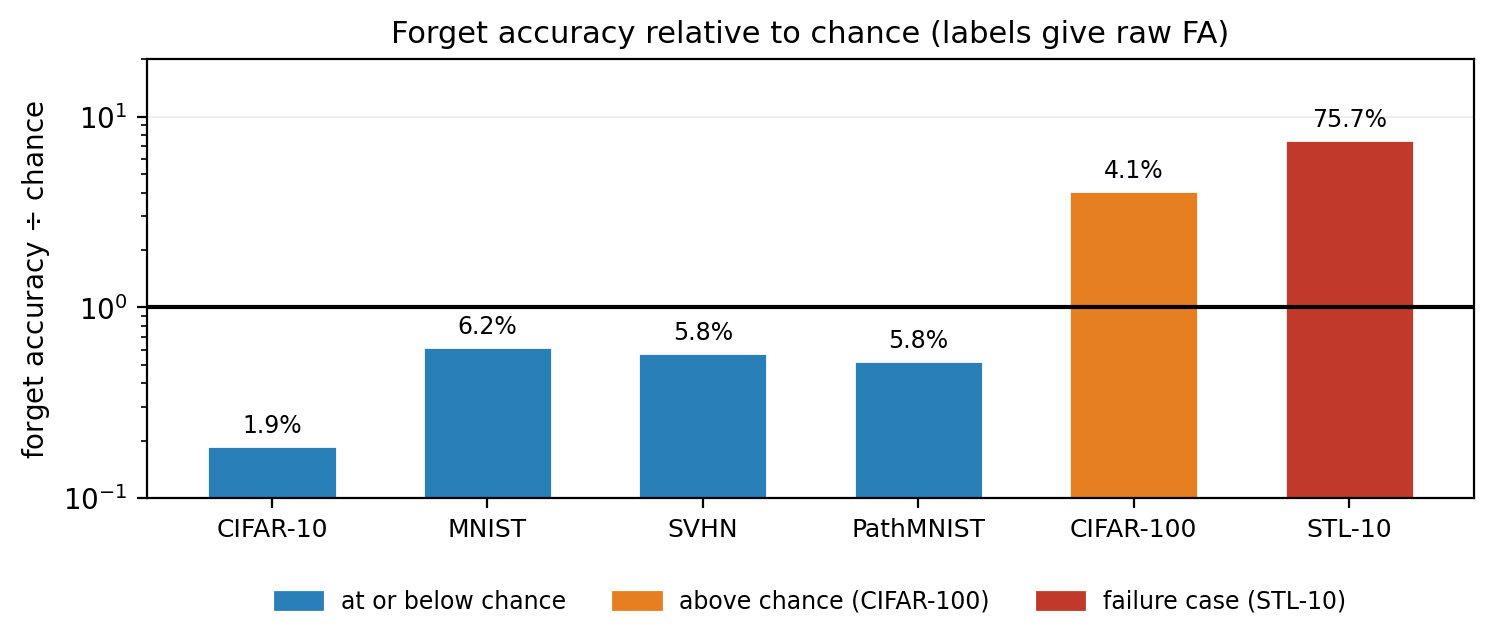
\includegraphics[width=0.86\textwidth]{fig_crossdataset.png}
\caption{\textbf{Forget accuracy relative to the chance level.} Raw forget
accuracy is not comparable across datasets: CIFAR-100's $4.1\%$ is
\emph{above} its $1\%$ chance level while MNIST's $6.2\%$ is \emph{below} its
$10\%$ one. Dividing by $100/K$ puts ``at chance'' at $1.0$ everywhere. Four
datasets sit below chance, CIFAR-100 above it despite a ${\sim}95$pp reduction,
and STL-10 above it at \rev{its 15-epoch cap, though not at 60 epochs}
(\S\ref{sec:crossdataset_stl}).}
\label{fig:crossdataset}
\end{figure}

\paragraph{The projection alone does not unlearn.}
The \emph{projection-only} row is the direct projected-gradient baseline: A-GEM
projection applied to plain gradient ascent, with the KD anchor and the
retain-confusion target removed. It preserves the retain set almost perfectly
($\mathrm{RA} = 99.90\%$), which is what the guarantee promises and all that it
promises---but it stops at $\mathrm{FA} = 18.66\%$, above the $10\%$ chance
level, and halts on the retain-loss budget rather than on the forget target.
Read together with the equal-compute ablation (Table~\ref{tab:ablation}), where
\emph{removing} the projection costs $47.4$pp of retain accuracy, this
delineates the division of labour precisely: the projection supplies retain
safety and nothing else, while the \klr{} objective is what actually drives
forget accuracy to chance. Neither component is sufficient alone, which is the
substantive content of the ablation.

\paragraph{CIFAR-100: scaling to 100 classes.}
Table~\ref{tab:cifar100} gives per-class results (base model TA~$=78.5\%$,
chance $=1\%$). \ours{} reduces FA from ${\sim}99\%$ to a mean of $4.07\%$
(median $1.60\%$) while holding RA at $92.19\%$, with MIA averaging $0.500$.
Eight of nine classes reach FA~$\le 6.8\%$; class~60 is an outlier at $17.8\%$
that does not converge within the 20-epoch budget, and it alone accounts for the
gap between the mean and the median (excluding it, mean FA is $2.35\%$). Unlike
the 10-class datasets, CIFAR-100 does not reach its $1\%$ chance level, so we
report it as a ${\sim}95$pp reduction rather than as forgetting to chance.

\begin{table}[t]
\centering
\caption{\textbf{CIFAR-100 class-level forgetting} (single seed per class,
chance $=1\%$). $^*$Class~60 does not converge within the 20-epoch budget.}
\label{tab:cifar100}
\begin{tabular}{@{}ccccc@{}}
\toprule
Forget class & TA (\%) & FA (\%)$\downarrow$ & RA (\%) & MIA \\
\midrule
10 & 77.23 & 4.20 & 92.84 & 0.485 \\
20 & 76.69 & 1.60 & 92.80 & 0.485 \\
30 & 75.18 & 1.40 & 91.03 & 0.486 \\
40 & 77.19 & 6.80 & 93.14 & 0.506 \\
50 & 76.25 & 0.60 & 92.31 & 0.562 \\
60$^*$ & 76.76 & 17.80 & 92.86 & 0.445 \\
70 & 75.38 & 1.60 & 90.89 & 0.482 \\
80 & 74.95 & 1.00 & 91.51 & 0.553 \\
90 & 75.87 & 1.60 & 92.32 & 0.498 \\
\midrule
\textbf{Mean} & \textbf{76.17} & \textbf{4.07} & \textbf{92.19} & \textbf{0.500} \\
\textbf{Median} & \textbf{76.25} & \textbf{1.60} & \textbf{92.31} & \textbf{0.486} \\
\bottomrule
\end{tabular}
\end{table}

\subsection{Momentum in Detail}\label{app:momentum}

The most direct route to an exact per-step guarantee is to remove momentum, so
that the applied update \emph{is} the projected gradient. Table~\ref{tab:momentum}
shows what that costs. With $\mu=0$ and all else fixed, \ours{} fails to forget
on five of six datasets: FA remains at $95.9\%$ on MNIST, $99.7\%$ on STL-10,
$73.7\%$ on CIFAR-100, and $61.9\%$ on SVHN. Retain accuracy stays high
throughout---but only because the model barely moves; high RA together with high
FA is the signature of a method that preserves retained knowledge by declining
to unlearn.

This is the empirical content of our central methodological claim. A per-step
guarantee stated for the momentum-free update would be exact and
implementation-matched, yet would describe a method that does not unlearn.
Projecting the post-momentum update instead keeps the guarantee exact
\emph{and} recovers forgetting on every dataset where it is attainable.

\begin{figure}[t]
\centering
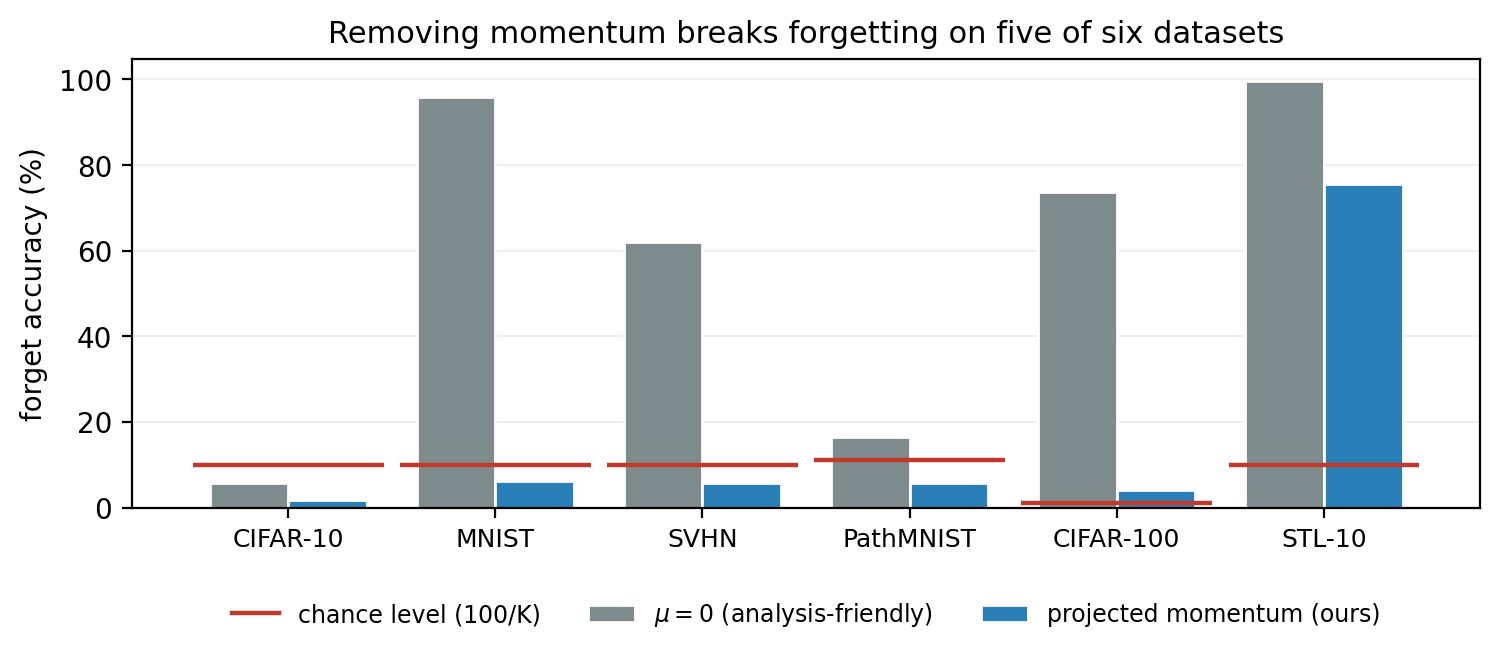
\includegraphics[width=0.86\textwidth]{fig_momentum.png}
\caption{\textbf{Momentum is not incidental.} Forget accuracy with momentum
removed ($\mu=0$, grey) against the projected-momentum update (blue), with each
dataset's chance level in red. The momentum-free configuration---the one for
which an exact guarantee is easiest to state---fails to forget on five of six
datasets. Retain accuracy stays high throughout (Table~\ref{tab:momentum}),
because the model barely moves.}
\label{fig:momentum}
\end{figure}

\paragraph{Is the dependence ours, or the field's?} A natural objection is that
this ablation only tells us something about \ours{}. If every gradient-based
unlearning rule collapses without momentum, the finding is about optimisers and
not about our design; if only ours does, the hard constraint is fragile. We
therefore repeated the ablation across four update rules on the two datasets
where Table~\ref{tab:momentum} shows the largest effect, at \emph{equal compute}
with stopping disabled so that the momentum change is not confounded with step
count (Table~\ref{tab:momentum_rules}).

\begin{table}[t]
\centering
\caption{\textbf{Where the momentum dependence comes from} (equal compute, 12
epochs on MNIST and 15 on SVHN, dual stopping disabled). $\Delta$ is the increase
in forget accuracy when momentum is removed, so larger is more dependent.
Grouping by forget objective separates the rows cleanly; grouping by whether the
projection is used does not.}
\label{tab:momentum_rules}
\begin{tabular}{@{}llcccc@{}}
\toprule
Update rule & Forget objective & Projection & MNIST $\Delta$ & SVHN $\Delta$ & mean \\
\midrule
\ours{}            & $\KL \to p_r$      & yes & $+95.3$ & $+62.4$ & $\mathbf{+78.8}$ \\
\texttt{kl\_uniform} & $\KL \to$ uniform & yes & $+84.9$ & $+56.3$ & $\mathbf{+70.6}$ \\
\addlinespace
projection only    & gradient ascent  & yes & $+16.5$ & $+13.2$ & $+14.8$ \\
gradient ascent    & gradient ascent  & no  & $+11.5$ & $+12.5$ & $+12.0$ \\
\bottomrule
\end{tabular}
\end{table}

Every rule degrades without momentum, including plain gradient ascent, which
uses no projection at all---so the dependence is not an artefact of operating
under a hard per-step constraint. But the rules do not degrade equally, and the
grouping is informative. The two KL-based objectives lose $70$--$79$pp of forget
accuracy on average, the two gradient-ascent objectives $12$--$15$pp: a factor
of $5.6$. Meanwhile the like-for-like comparison that isolates the
projection---gradient ascent with it ($+14.8$) against gradient ascent without
it ($+12.0$)---differs by only $2.8$pp.

The momentum dependence therefore belongs to the \emph{forget objective}, not to
the projection. The reason is visible in the objective itself: $\KL(p_\theta(x_f)
\| p_r)$ is bounded and its gradient vanishes as $p_\theta \to p_r$, so the
per-step signal is small and the $1/(1-\mu) = 10\times$ amplification that
momentum supplies (Lemma~\ref{lem:vel}) is what makes progress possible at
all. Gradient ascent maximises an unbounded loss and needs no such
amplification, which is also why it damages the retained model.

This sharpens rather than weakens the section's claim. The point was never that
momentum is uniquely important to \ours{}; it is that the guarantee must be
stated for the update the optimiser applies, and any method whose objective
requires momentum inherits that requirement. A momentum-free analysis is
convenient for exactly the objectives that cannot afford to be momentum-free.

\subsection{Auditing the Guarantee at Step Level}\label{sec:alignment}

We log every gradient step of a CIFAR-10 class-0 run (120 steps) and check
Theorem~\ref{thm:retain_safety} directly rather than assuming it.

\begin{itemize}
\item \textbf{The constraint is active, not vacuous.} All $120/120$ steps have
$\langle v_t,\gr\rangle < 0$, so the projection fires at every step. Projection
here is not an occasional correction: without it, every step would increase
retain loss to first order.
\item \textbf{The guarantee holds.} After projection,
$\langle u_t,\gr\rangle \ge 0$ at every step to floating-point precision. The
largest relative violation is
$\langle u_t,\gr\rangle/(\|u_t\|\|\gr\|) = -7.4\times 10^{-7}$, against a
float32 accumulation scale of ${\sim}4\times 10^{-4}$ for sums over 11.2M
parameters; the mean relative alignment is positive
($+2.2\times 10^{-8}$). The implied worst-case first-order retain increase is
$3.1\times 10^{-7}$, three orders of magnitude below the observed per-step
retain-loss fluctuation ($1.8\times 10^{-4}$). We therefore state the guarantee
as holding to float32 precision, and recommend float64 accumulation for the
inner products in reference implementations.
\item \textbf{The norm bound is respected.} $\|u_t\|$ reaches a maximum of
$9.16$ against the theoretical bound $c/(1-\mu)=10$, with mean $7.35$---close to
but never exceeding the bound, confirming both that the bound is tight and that
momentum's amplification is being realised.
\item \textbf{Retain loss is controlled.} The mean per-step change in mini-batch
retain CE is $-7.9\times 10^{-5}$ (i.e.\ decreasing), with a maximum single-step
increase of $+1.05\times 10^{-3}$, consistent with the $O(\eta^2)$ term of
Eq.~\ref{eq:thm1}.
\end{itemize}

\subsection{BatchNorm Recalibration in Detail}\label{app:bn}

Table~\ref{tab:gn} reports \ours{} with a GroupNorm backbone across datasets.
GroupNorm keeps forgetting intact on four of five datasets at a modest TA cost
(e.g.\ CIFAR-10 $84.16\%$ vs $86.13\%$), while removing the BN-recalibration
mechanism by construction, since there are no batch statistics to recalibrate.
STL-10 is under-trained under GroupNorm as it is under BN, at \rev{its epoch cap}
(\S\ref{sec:crossdataset_stl}).

\begin{table}[t]
\centering
\caption{\textbf{\ours{} with a GroupNorm backbone} (3-seed means). GroupNorm
removes the BN-recalibration vulnerability structurally. $^*$STL-10 is under-trained under
both backbones.}
\label{tab:gn}
\begin{tabular}{@{}lcccc@{}}
\toprule
\textbf{Dataset} & \textbf{TA} & \textbf{FA}$\downarrow$ & \textbf{RA} & \textbf{MIA} \\
\midrule
CIFAR-10    & 84.16 & 3.44 & 99.23 & 0.478 \\
MNIST       & 90.17 & 5.84 & 99.31 & 0.500 \\
SVHN        & 87.99 & 3.46 & 95.49 & 0.581 \\
STL-10$^*$  & 83.92 & 97.60 & 92.95 & 0.552 \\
PathMNIST   & 72.00 & 2.71 & 95.97 & 0.583 \\
\bottomrule
\end{tabular}
\end{table}

Table~\ref{tab:bnrecal} reports the diagnostic itself. The operator is
\texttt{torch.optim.swa\_utils.update\_bn} applied to the retain set: it resets
every BatchNorm buffer, sets the momentum to \texttt{None} so that PyTorch
accumulates a cumulative rather than exponential average, and runs forward
passes with no backward pass and no weight update. The resulting statistics are
therefore the exact retain-set statistics, independent of the pre-attack buffers
and idempotent in the data. We verify after every run that all learnable
parameters are bit-identical, so nothing but the buffers can have changed. Then
$\Delta F = \mathrm{post} - \mathrm{pre}$ separates weight-level forgetting
($\Delta F \approx 0$) from forgetting mediated by batch statistics
($\Delta F \gg 0$). We also report a weaker variant---forward passes in
\texttt{train} mode under the default exponential average, which is what an
earlier version of this work used---and the two agree to within $1.2$pp on every
row, and to $0.02$pp on the \ours{} row that carries the finding, so the choice
of estimator is not what drives the result. All
accuracies here are measured under deterministic (test-time) transforms; leaving
training augmentation active perturbs individual rows by several points.



\paragraph{The vulnerability is ours, not the field's---in our reproductions.}
The baseline rows matter more than \ours{}'s. Every one of them is unaffected by
recalibration---the largest movement is SCRUB's $-3.6$pp, in the direction of
\emph{more} forgetting---and so is the base model, which is the control that
matters: recalibrating a normally trained network changes nothing, because its
statistics already agree with its weights. Only \ours{} carries a mismatch.
$\Delta F = +98.4$pp means the attack does not merely degrade the unlearning but
\emph{undoes} it: forget accuracy returns to $99.7\%$ and test accuracy to
$92.9\%$\rev{---the values recalibration gives the base model itself ($99.8\%$
and $92.9\%$)}---without a single weight being modified. On a BatchNorm backbone, what \ours{} produces is not an
unlearned model but an unlearned model's statistics.

We qualify the first half of that heading deliberately. \rev{Concurrent work
\citep{kalani2026batchnorm} reports large recoveries for SalUn ($+62.1$pp) and
Bad Teacher ($+78.2$pp) under their reference implementations, where we measure
none. We ran the identical operator, so the disagreement is not in the attack
but in how the unlearned checkpoints were produced. Our implementations end
every epoch with a full pass over retained data in train mode, which recomputes
the running statistics before the checkpoint is saved; \citet{kalani2026batchnorm}
run Bad Teacher's BatchNorm in eval mode, and find that SalUn's recovery
disappears once at least a quarter of each unlearning batch is retained data.}
Our claim is therefore that the vulnerability is \ours{}-specific \emph{among
the checkpoints we trained}, not that these baselines are immune in general.

We attribute it, tentatively, to the interaction between our own design choice
and BatchNorm. \ours{} freezes the normalisation statistics during unlearning so
that class-homogeneous forget batches cannot corrupt them; the weights therefore
adapt against \emph{fixed} statistics, and the resulting decision boundary is
valid only for those statistics. Methods that let the statistics move during
unlearning never build that dependence. Freezing BatchNorm is thus necessary but
not sufficient: it prevents the statistics from manufacturing apparent
forgetting, and simultaneously makes the weights depend on them.
\added{Section~\ref{sec:bn_robust} puts this attribution to an interventional
test: keeping the statistics consistent with the weights throughout unlearning
removes the vulnerability.}

The GroupNorm backbone removes the mechanism by construction---there are no batch
statistics to recalibrate---at a cost of $2.0$pp of test accuracy
(Table~\ref{tab:gn}). The ViT-B/16 backbone
(\S\ref{sec:vit}) does the same for a different reason: LayerNorm normalises
per example at inference and keeps no running statistics either. Two
architectures with unrelated designs are both outside the operator's reach, and
both unlearn properly, which locates the defect in the normalisation scheme
rather than in gradient projection.

We state the limit of that plainly: neither backbone \emph{resists} the attack,
because the attack is undefined on them. This is a design change, not
demonstrated robustness, and a method that must avoid BatchNorm to be safe is
constrained in a way the guarantee itself does not capture. What the two rows do
establish is that the defect is separable from \ours{}'s mechanism---it is a
property of freezing statistics that a normalisation layer keeps, and it
disappears wherever there are no such statistics. \added{The next subsection
removes the constraint itself: it keeps BatchNorm, and makes \ours{} robust to
the attack rather than outside its reach.}

\begingroup\color{revised}% ---- new subsection: everything to \endgroup is added
\subsection{BN-robust \ours{} in Detail}\label{app:bn_robust}

The diagnosis above points at its own remedy: if the weights learn to forget
against statistics that are allowed to go stale, the statistics should never be
stale. BN-robust \ours{} makes three changes to Algorithm~\ref{alg:excise}
(Figure~\ref{fig:bnrobust_mech}). It leaves the update rule untouched, \rev{so
Theorem~\ref{thm:retain_safety} holds at every step for the retain objective
under the statistics in force during that step; the recalibration between steps
is not covered by it}.
\begin{enumerate}
\item \emph{Track the weights.} Before every step the BatchNorm statistics are
recomputed, $\phi \leftarrow R(\theta, B_r)$, with the attacker's own operator
$R$ (\texttt{update\_bn}) on a fresh sample $B_r$ of $512$ retain images. The
step's forward and backward passes then run under statistics consistent with the
current weights. Forget batches still never touch the statistics: this keeps
the half of freezing that was right and drops the half that was wrong.
\item \emph{Ship consistent statistics.} After the last step,
$\phi \leftarrow R(\theta_T, \Dr)$ on the whole retain set under test-time
transforms---exactly what the attacker computes.
\item \emph{Stop on the forget accuracy that ships.} The stopping rule of
\S\ref{sec:stopping} reads FA under $R(\theta, \Dr)$ with test-time transforms,
not under the in-loop statistics. If the target is not met within the epoch
budget, the epoch with the lowest such FA inside the retain budget is shipped
instead of the last one.
\end{enumerate}
\begin{figure}[t]
\centering\color{revised}
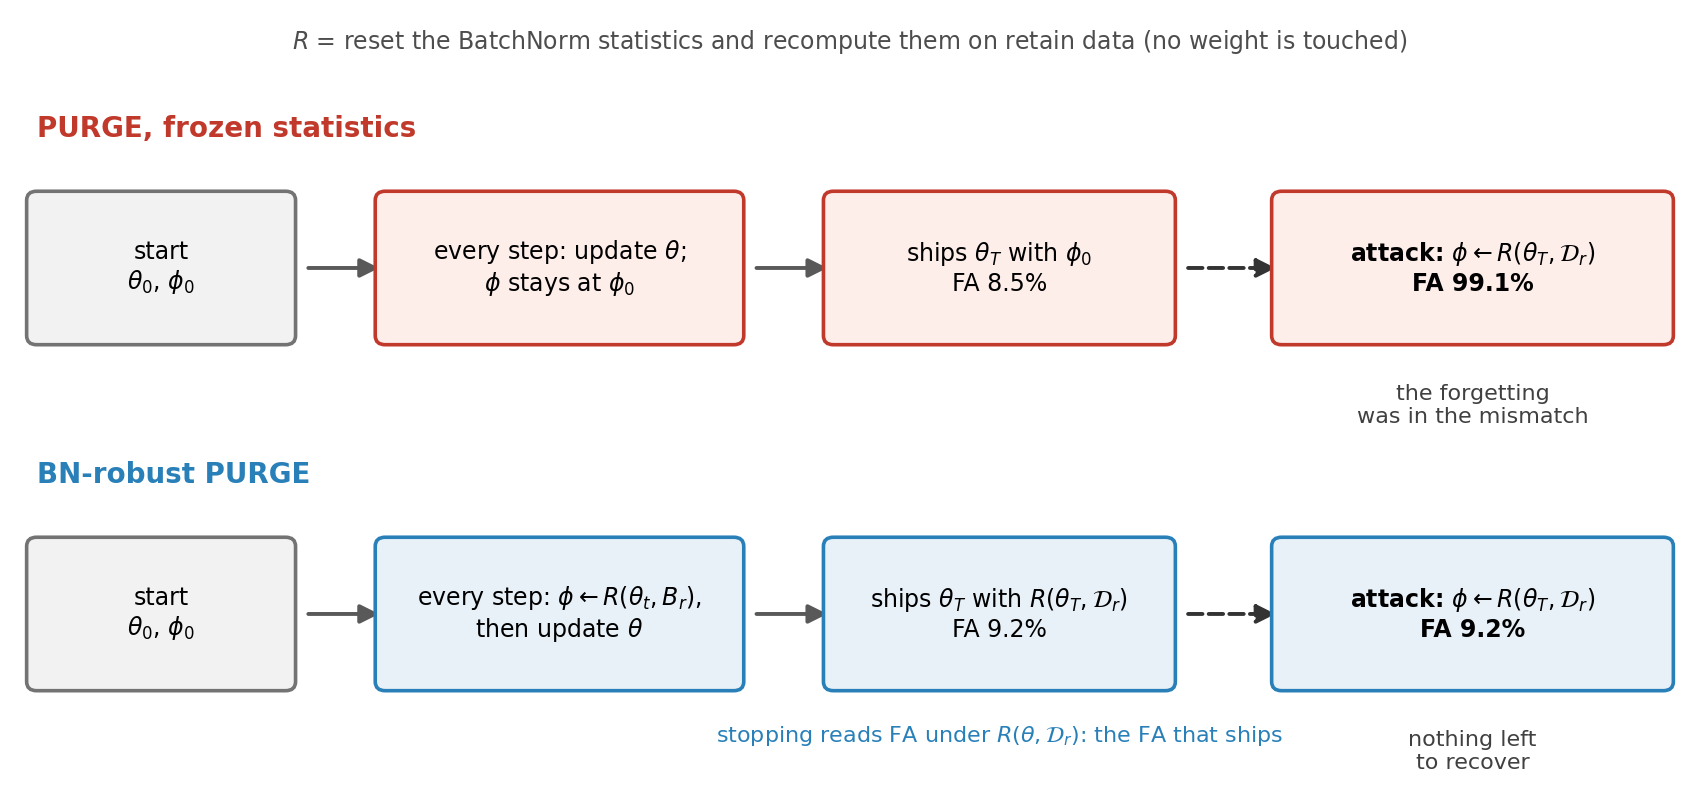
\includegraphics[width=\textwidth]{fig_bnrobust_mechanism.png}
\caption{\added{\textbf{What BN-robust \ours{} changes.} $R$ resets the BatchNorm
statistics and recomputes them on retain data without touching a weight. With
frozen statistics the forgetting lives in the mismatch between $\theta_T$ and
$\phi_0$, and the attack removes it; BN-robust ships statistics consistent with
its weights, so the attack has nothing to recover. Forget accuracies are
CIFAR-10 class~0, means over three seeds (Table~\ref{tab:bnrobust}).}}
\label{fig:bnrobust_mech}
\end{figure}

Because $R$ is idempotent, change~2 makes the attack a no-op on the shipped model
by construction, so $\Delta F = 0$ is not by itself evidence here. The question
this variant must answer is whether FA is still low once $\phi$ cannot be
stale. Two of the tests below are not no-ops by construction: the
exponential-average operator, and recalibration on data other than the retain
set.

Change~3 is not cosmetic. Without it, the FA that triggers stopping is read under
the in-loop statistics---a few hundred augmented images, one step behind---on
augmented forget images. On CIFAR-10 that reading falls short of the shipped FA
by between $-1.0$ and $+9.0$pp depending on the class, and runs stopped at
``FA $\le 10\%$'' shipped at $7.2$--$16.7\%$ (Figure~\ref{fig:bnrobust_stop}). With change~3 the shipped FA meets
the target, and the seed-to-seed spread on class~0 falls from $1.90$ to
$0.08$pp (Table~\ref{tab:bnrobust}). The stopping check need not use the whole
retain set. Computing it on $10{,}240$ images reproduced every stopping decision
of the full check on all three seeds and cut wall-clock by $16\%$; the shipped
statistics still use the full set.

\begin{figure}[t]
\centering\color{revised}
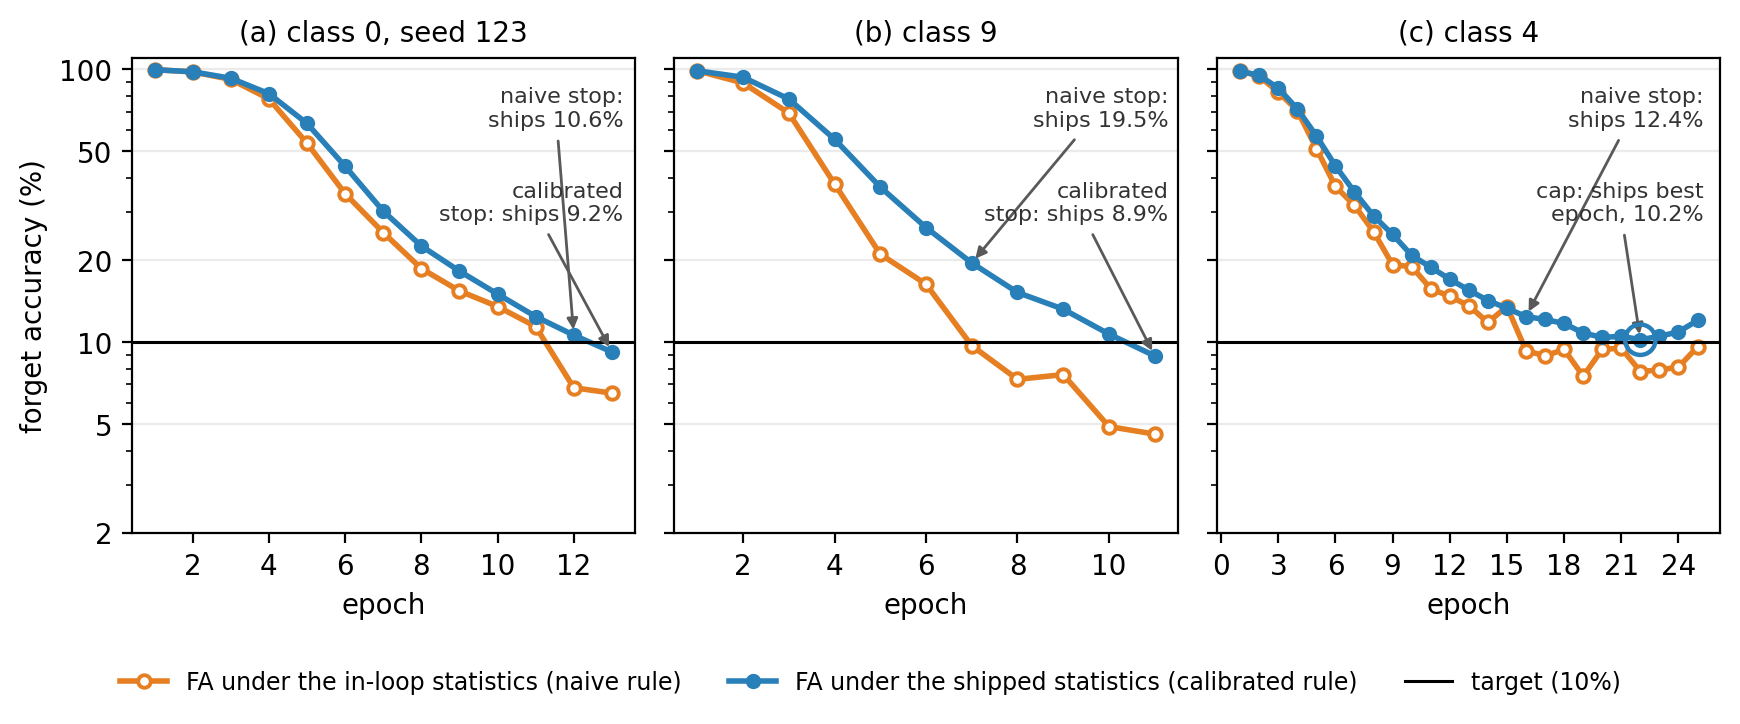
\includegraphics[width=\textwidth]{fig_bnrobust_stopping.png}
\caption{\added{\textbf{Why stopping must be calibrated.} Forget accuracy per epoch
under the in-loop statistics (what naive stopping reads) and under the
statistics that ship (what calibrated stopping reads); log scale. The in-loop
reading runs below the shipped one, so a naive rule stops early and ships above
chance: (a)~one epoch early on class~0, (b)~four epochs early on class~9,
shipping $19.5\%$ instead of $8.9\%$. (c)~On class~4 the shipped FA plateaus just
above $10\%$ and the run reaches the epoch cap; the best-epoch rule ships epoch~22
($10.2\%$) rather than the last ($12.0\%$).}}
\label{fig:bnrobust_stop}
\end{figure}

These experiments were run after the checkpoints behind
Table~\ref{tab:bnrecal} became unavailable. They use an earlier CIFAR-10 base
(test accuracy $93.97\%$, against $95.5\%$ there), a GroupNorm base retrained for
$100$ rather than $200$ epochs ($91.89\%$), and a retrained MNIST base
($99.59\%$). Their absolute numbers are therefore not comparable row for row
with the rest of \S\ref{sec:experiments}; every comparison below is between arms
that share a base.



\paragraph{It survives the attack it was built against, and two it was not.}
Calibrated BN-robust forgets class~0 to $9.19\%$ and stays at $9.18\%$ under
recalibration (Figure~\ref{fig:bnrobust_attack}a), while the frozen configuration
returns to $99.12\%$ with test accuracy back at $94.1\%$---the original model. The exponential-average
operator, which is not idempotent and therefore not a no-op here, moves
BN-robust by at most $+0.3$pp. Nor does robustness depend on the attacker using
the retain set. On the naive-stopping checkpoints, recomputing the statistics
on the full training set, forget class included, or on the test set---data
BN-robust never trained under---moves its FA by $-1.0$ to $-1.2$pp, towards more
forgetting, while the frozen configuration still recovers to $97.4\%$ and
$97.3\%$ (Figure~\ref{fig:bnrobust_attack}b).

\paragraph{Every class, and a second dataset.}
On all ten CIFAR-10 classes (seed~$42$; Table~\ref{tab:app_bnrobust} and
Figure~\ref{fig:app_bnrobust}), the
frozen configuration recovers to $94.7$--$99.3\%$ under the attack, while
BN-robust's FA moves by at most $0.06$pp under either stopping rule. With
calibrated stopping every class ships between $6.7\%$ and $10.2\%$, inside three
standard errors of chance ($11.3\%$ for $5{,}000$ images); with naive stopping,
five of the ten did not. One class needed the fallback. Class~4 hovered at
$10.2$--$10.9\%$ for six epochs without crossing $10\%$ and reached the epoch
cap, and the rule shipped its best epoch ($10.2\%$) rather than the last
($11.9\%$, with retain accuracy $1.4$pp lower). On MNIST, over three seeds, the
frozen configuration's forgetting is undone completely ($0.00\% \to 99.97\%$,
with test accuracy back to $99.56\%$ against the base's $99.59\%$), and
BN-robust holds ($3.78\% \to 3.87\%$, test accuracy $90.10\%$).

\paragraph{What it costs, and why it is slower.}
Against the frozen configuration, BN-robust gives up $1.8$pp of retain accuracy
and $0.9$pp of test accuracy and takes about seven times the wall-clock, most of
it because it needs $13$ epochs instead of $2$. We read the slower forgetting as
the substance rather than the overhead. The frozen configuration reaches its
target in two epochs largely through the statistics mismatch, which the attack
shows is not forgetting at all; once the statistics track the weights, the
forgetting has to happen in the weights. BN-robust's test accuracy, $84.30\%$,
is close to the $84.6\%$ expected from removing one class of ten from a
$93.97\%$ model. Against GroupNorm, BN-robust keeps $1.2$pp more test accuracy,
mostly because it can start from the stronger BatchNorm base, and it needs
neither a change of architecture nor a retrained base model.
Membership-inference AUROC stays between $0.48$ and $0.52$ for every unlearned
row.

\paragraph{What it does and does not establish.}
Unlike GroupNorm or a transformer, this is robustness rather than immunity by
construction: the attack is defined on the model, runs, and finds nothing to
recover. It is robustness to one attack, though. BN-robust changes only how the
normalisation statistics are maintained, so it does nothing against attacks that
modify the weights, such as fine-tuning recovery (\S\ref{sec:limitations}), and
we have tested it on two datasets rather than six. Within that scope, \ours{} no
longer has to choose between BatchNorm and its forgetting: BN-robust \ours{},
\ours{} with GroupNorm, and \ours{} on a transformer are all configurations we
would deploy.
\endgroup% ---- end of the added subsection

\subsection{A Transformer Backbone}\label{sec:vit}

Every result so far uses ResNet-18, so the projection has only ever been applied
to a convolutional network. We repeat CIFAR-10 class~0 on ViT-B/16 under the
identical algorithm, with representation erasure disabled as everywhere else,
over three seeds.

\begin{table}[t]
\centering
\caption{\textbf{ViT-B/16 against ResNet-18}, same algorithm and forget targets
as Table~\ref{tab:cross}\rev{; the ViT runs check forget accuracy every step.
Chance is $10\%$ on CIFAR-10 and $1\%$ on CIFAR-100. The projection fires on
$98$--$100\%$ of steps, as it does on ResNet-18.}}
\label{tab:vit}
\begin{tabular}{@{}lcccc@{}}
\toprule
Backbone & TA & FA$\downarrow$ & RA & MIA \\
\midrule
\multicolumn{5}{@{}l}{\rev{\emph{CIFAR-10, class~0, three seeds}}} \\
ResNet-18 (Table~\ref{tab:cross}) & $86.13 \pm 0.02$ & $1.87 \pm 0.25$ & $100.00 \pm 0.00$ & $0.529$ \\
ViT-B/16                          & $87.05 \pm \rev{0.09}$ & $9.71 \pm \rev{0.27}$ & $\phantom{0}97.55 \pm \rev{0.10}$ & $0.453$ \\
\midrule
\multicolumn{5}{@{}l}{\rev{\emph{CIFAR-100, classes $10,\dots,90$, one seed each, 20-epoch cap}}} \\
\rev{ResNet-18 (Table~\ref{tab:cross})} & \rev{$76.17 \pm 0.86$} & \rev{$4.07 \pm 5.51$} & \rev{$92.19 \pm 0.84$} & \rev{$0.500$} \\
\rev{ViT-B/16} & \rev{$81.97 \pm 0.66$} & \rev{$24.00 \pm 23.16$} & \rev{$91.86 \pm 0.73$} & \rev{$0.435$} \\
\bottomrule
\end{tabular}
\end{table}

\rev{On CIFAR-10} forgetting transfers: FA reaches $9.71\%$, below the $10\%$
chance level, with retain accuracy at $97.55\%$ and test accuracy slightly
\emph{above} the ResNet-18 result. The gap in FA against ResNet-18's $1.87\%$ is not a weaker
result but a different stopping point---both runs use $\tau_F = 10\%$, and
the ViT run halts as soon as it crosses that threshold (epoch~3, mid-epoch),
whereas the ResNet-18 run overshoots it. \S\ref{sec:experiments} shows that
overshoot is an artifact of check granularity rather than a property of either
backbone.

\rev{On CIFAR-100 it does not transfer within the same 20-epoch cap. On the nine
classes of Table~\ref{tab:cross}, ViT-B/16 ends with FA between $4.0\%$ and
$82.0\%$ (mean $24.0\%$) against a $1\%$ chance level, so no class reaches
chance, where ResNet-18 ends at $4.07\%$ and reaches chance at 60 epochs.
Retain accuracy ($91.9\%$) matches ResNet-18's. We have not tested whether a
longer budget closes the gap, as it does for ResNet-18; until then the
transformer result holds for CIFAR-10 only.}

Two things follow. First, the conflict the projection resolves is not an artifact
of convolutional architectures: the projection fires on $99$--$100\%$ of steps
here as well, so forget and retain gradients oppose one another just as
routinely in a transformer. Second, and more usefully,
ViT normalises with LayerNorm, which computes statistics per example at
inference and stores none. It is therefore outside the reach of the
recalibration operator of \S\ref{sec:bn_results} for the same structural reason
as GroupNorm, but by way of a completely different architecture---which is what
makes the pair informative rather than merely repetitive.

\subsection{Component Ablation}\label{sec:ablation}

A component ablation run in the deployed configuration is uninformative here,
and the reason is instructive. Under the projected-momentum optimiser every
variant reaches the forget-accuracy target inside the first check interval, so
dual stopping halts them all after one epoch and each looks equally good: in the
upper half of Table~\ref{tab:ablation}, removing the projection costs
$0.09$pp of retain accuracy. That number is an artefact of stopping, not a
measurement of what the projection does.

We therefore also run every variant at \emph{equal compute}, with stopping
disabled throughout (lower half). The picture inverts.

\begin{table}[t]
\centering
\caption{\textbf{Component ablation} (CIFAR-10 class~0, seed 42). Upper: the
deployed configuration, where dual stopping halts every variant after one epoch.
Lower: equal compute, 15 epochs, stopping disabled for all variants---the same
comparison without the stopping confound. \texttt{+rep} and \texttt{+gate}
re-introduce the two components removed in \S\ref{sec:method}.}
\label{tab:ablation}
\begin{tabular}{@{}llcccc@{}}
\toprule
& Variant & TA & FA & RA & MIA \\
\midrule
\multirow{7}{*}{\rotatebox{90}{\emph{stopping on}}}
 & full \ours{}      & $86.10$ & $2.14$ & $100.00$ & $0.528$ \\
 & $-$KD             & $85.56$ & $0.80$ & $99.99$  & $0.516$ \\
 & $-$projection     & $84.87$ & $0.78$ & $99.91$  & $0.513$ \\
 & selective-layer   & $86.26$ & $3.26$ & $100.00$ & $0.528$ \\
 & $+$rep            & $86.10$ & $2.14$ & $100.00$ & $0.528$ \\
 & $+$gate           & $86.10$ & $2.14$ & $100.00$ & $0.528$ \\
 & $-$stopping       & $85.71$ & $0.00$ & $99.98$  & $0.472$ \\
\midrule
\multirow{6}{*}{\rotatebox{90}{\emph{equal compute}}}
 & full \ours{}      & $85.70$ & $0.00$ & $99.98$  & $0.472$ \\
 & $-$KD             & $85.66$ & $0.00$ & $99.94$  & $0.475$ \\
 & $-$projection     & $\mathbf{44.37}$ & $0.00$ & $\mathbf{52.55}$ & $0.436$ \\
 & selective-layer   & $85.76$ & $0.00$ & $99.99$  & $0.469$ \\
 & $+$rep            & $85.74$ & $0.00$ & $99.98$  & $0.473$ \\
 & $+$gate           & $87.16$ & $19.28$ & $100.00$ & $0.539$ \\
\bottomrule
\end{tabular}
\end{table}

\paragraph{The projection is what makes unlearning survivable.}
At equal compute, removing it costs $41.3$pp of test accuracy and
$47.4$pp of retain accuracy: the model collapses to $44.4/52.6$ against
$85.7/99.98$ for the full method. This is the empirical counterpart of
Theorem~\ref{thm:retain_safety}, and it is a far larger effect than the
stopping-confounded comparison suggests. Note also that the two rows disagree
about the \emph{sign} of the conclusion---one reports the projection as
costless, the other as indispensable---which is why we report both rather than
whichever is more favourable.

\paragraph{KD contributes little once compute is equalised.}
Removing the distillation anchor changes retain accuracy by $0.04$pp at equal
compute. We previously attributed several points of retain accuracy to it; that
is not supported here, and we no longer claim it.

\paragraph{The removed components stay removed.}
Re-introducing representation erasure reproduces the full method to within
$0.04$pp on every metric, and re-introducing the entropy gate leaves forget
accuracy at $19.3\%$---above the $10\%$ chance level, i.e.\ it prevents the
method from forgetting. Both were dropped in \S\ref{sec:method} on the strength
of an ablation run under the previous implementation; this re-run confirms the
decision under the current one.

\subsection{How Hard Must the Constraint Be?}\label{sec:strength}

Theorem~\ref{thm:separation}(iv) argues that a soft conflict penalty biases the
update without excluding retain-harming steps, and that only a hard constraint
makes them unreachable. That is an argument about feasible sets; here we measure
what it costs in practice. We interpolate the projection with a strength
parameter $s$: at each conflicting step the update becomes
$u_t = v_t - s\,\frac{\langle v_t,\gr\rangle}{\|\gr\|^2}\gr$, so
\begin{equation}\label{eq:strength}
\langle u_t, \gr\rangle \;=\; (1-s)\,\langle v_t, \gr\rangle .
\end{equation}
At $s=0$ nothing is corrected; at $s=1$ this is \ours{}. Every intermediate
value is a soft penalty---it shrinks the conflicting component without removing
it---and by Eq.~\ref{eq:strength} it leaves $\langle u_t,\gr\rangle<0$ whenever
the raw update conflicts. All other settings are held fixed, and stopping is
disabled so that every variant sees the same compute.

\begin{table}[t]
\centering
\caption{\textbf{Projection strength} (CIFAR-10 class~0, equal compute, stopping
disabled). $s=0$ applies no correction, $s=1$ is the full hard constraint.
Forget accuracy is $0.0\%$ throughout, so the runs differ only in collateral
damage.}
\label{tab:strength}
\begin{tabular}{@{}lccccc@{}}
\toprule
$s$ & residual conflict & TA & FA & RA & MIA \\
\midrule
$0.00$ & $1.00\,\langle v_t,\gr\rangle$ & $44.35$ & $0.0$ & $52.54$ & $0.436$ \\
$0.25$ & $0.75\,\langle v_t,\gr\rangle$ & $67.84$ & $0.0$ & $81.35$ & $0.497$ \\
$0.50$ & $0.50\,\langle v_t,\gr\rangle$ & $78.03$ & $0.0$ & $92.75$ & $0.510$ \\
$0.75$ & $0.25\,\langle v_t,\gr\rangle$ & $82.99$ & $0.0$ & $98.24$ & $0.509$ \\
$1.00$ & $\mathbf{0}$ & $\mathbf{85.71}$ & $0.0$ & $\mathbf{99.98}$ & $0.472$ \\
\bottomrule
\end{tabular}
\end{table}

\begin{figure}[t]
\centering
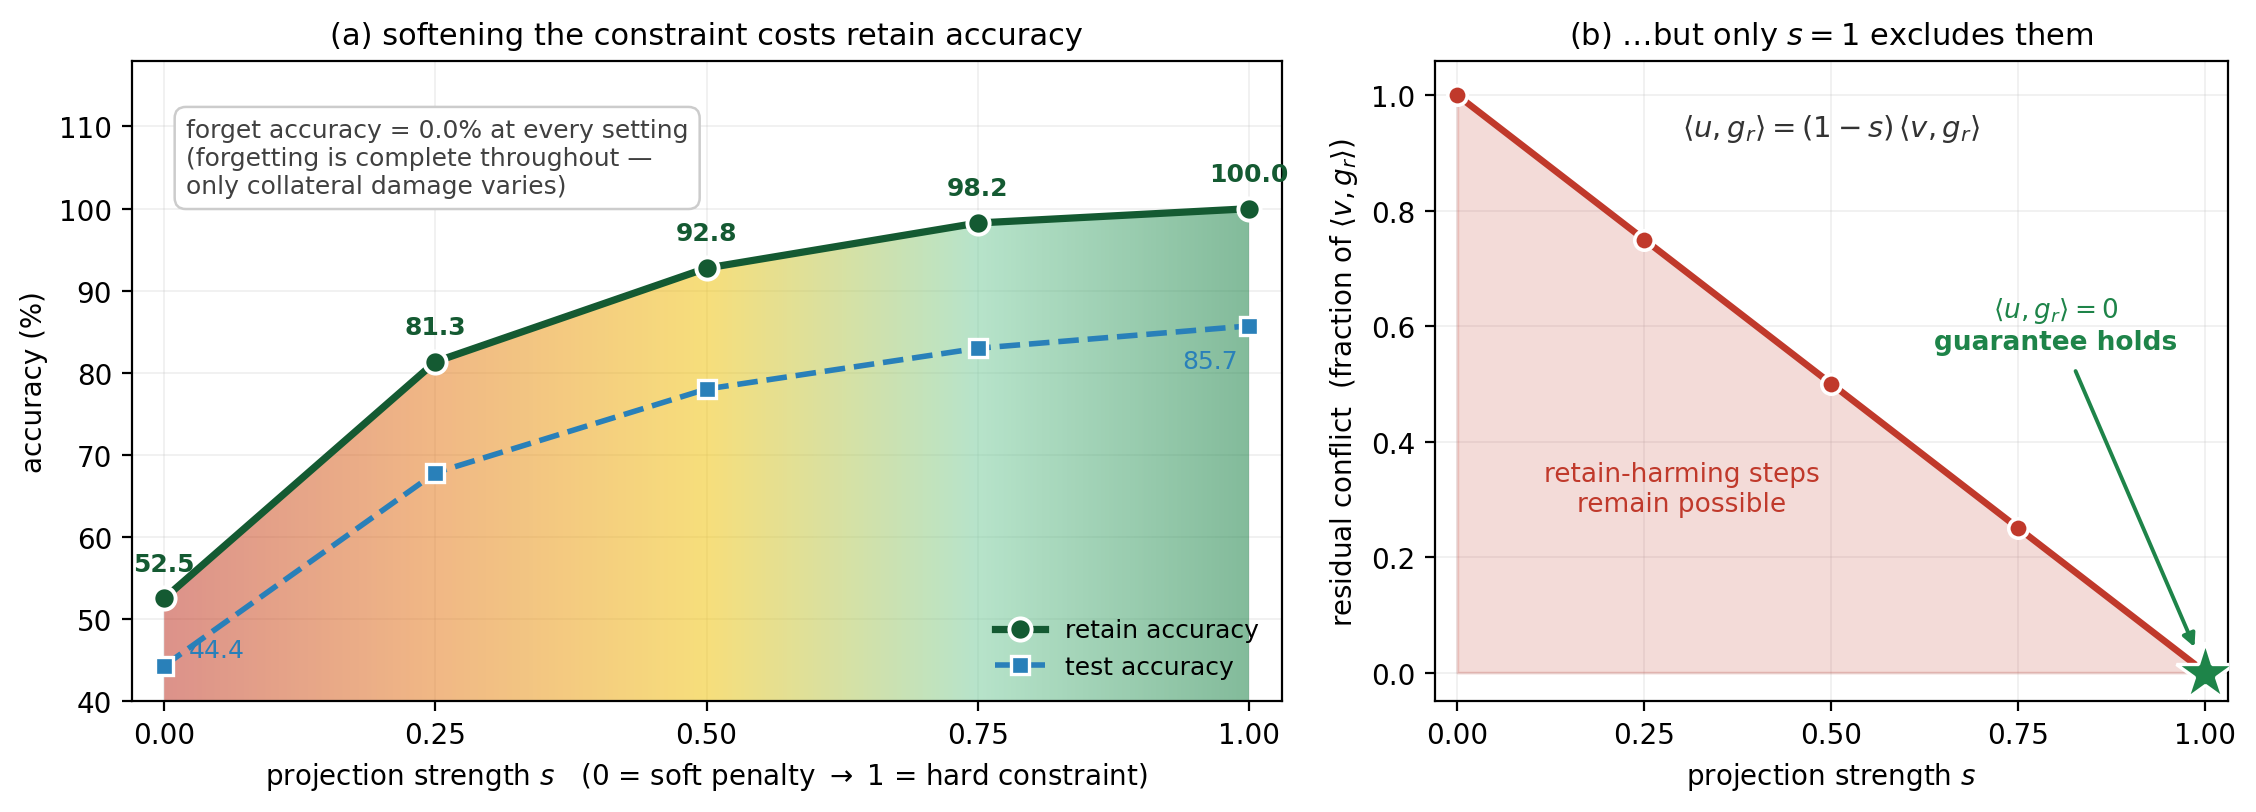
\includegraphics[width=\textwidth]{fig_strength.png}
\caption{\textbf{Hardening the constraint recovers retain accuracy
continuously, but only the endpoint carries the guarantee.}
\textbf{(a)}~Retain and test accuracy against projection strength; forget
accuracy is $0.0\%$ at every setting, so the runs differ only in collateral
damage. \textbf{(b)}~Residual conflict $(1-s)$: retain-harming steps remain
reachable for every $s<1$ and are excluded only at $s=1$. The empirical
difference between $s=0.75$ and $s=1$ is $1.7$pp of retain accuracy; the
difference in what can be proved is categorical.}
\label{fig:strength}
\end{figure}

\paragraph{Softening is expensive, and monotonically so.}
Retain accuracy falls from $99.98\%$ at $s=1$ to $52.54\%$ at $s=0$, and test
accuracy from $85.71\%$ to $44.35\%$, monotonically in between. Because forget
accuracy is $0.0\%$ at every setting, this is not a privacy--utility trade-off:
all five runs forget equally, and they differ only in how much of the retained
model they destroy on the way. The $s=0$ row reproduces the equal-compute
$-$projection ablation of Table~\ref{tab:ablation} from an independent
direction.

\paragraph{The curve is gradual, which we take as a limitation of the empirical
argument.} Most of the benefit arrives early---$s=0.25$ already recovers
$28.8$pp of retain accuracy, while the final quarter, $s=0.75\to1$, is worth
$1.7$pp. A soft penalty tuned near $s=0.75$ therefore performs almost as well as
the hard constraint on these metrics, and we do not claim otherwise. What it
does not do is satisfy Eq.~\ref{eq:strength} with equality: at $s=0.75$ a
quarter of every conflict survives into the applied update, so
$\langle u_t,\gr\rangle<0$ on conflicting steps and no per-step statement can be
made. The case for $s=1$ is therefore not that the last $1.7$pp is large, but
that it is the only setting about which anything can be proved---which is the
whole content of Theorem~\ref{thm:retain_safety}.

\paragraph{Relation to soft conflict-resolution methods.}
This is a controlled test of the mechanism that separates \ours{} from the
closest prior work \citep{patel2025learning}, not a comparison with that method:
it varies our own projection rather than reimplementing theirs, and their
penalty acts on the objective rather than on the update. What it establishes is
the general shape of the trade---that discouraging conflict helps in proportion
to how much of it is removed, and that removing all of it is what converts an
empirical tendency into a guarantee. A like-for-like comparison remains future
work (\S\ref{sec:limitations}).

\subsection{Privacy--Utility Frontier and Robustness Diagnostics}\label{sec:sweeps}

We sweep the two tolerances of Eq.~\ref{eq:problem} independently on CIFAR-10
class~0 (Table~\ref{tab:sweeps}). The results are asymmetric: one tolerance is
inert because the projection has already done its work, while the other is
genuinely active but was hidden by how coarsely we measured it.

\begin{table}[t]
\centering
\caption{\textbf{Tolerance sweeps} (CIFAR-10 class~0). Sweep~A varies the
retain-loss budget $\alpha$ at fixed $\tau_F = 10\%$; Sweeps~B and B$'$ vary
the forget-accuracy target $\tau_F$ at fixed $\alpha = 5$, checking forget
accuracy every 50 batches and every step respectively. $\alpha$ is inert. So is
$\tau_F$ under the coarse check---but only because forget accuracy crosses
the whole range between two consecutive checks; measured per step, it tracks the
requested tolerance across a $29$pp range.}
\label{tab:sweeps}
\begin{tabular}{@{}lccccc@{}}
\toprule
\multicolumn{2}{@{}l}{Sweep A: $\alpha$} & TA & FA & RA & MIA \\
\midrule
& $1.5$    & $86.10$ & $1.88$ & $100.00$ & $0.530$ \\
& $2$      & $86.10$ & $1.88$ & $100.00$ & $0.530$ \\
& $3$      & $86.10$ & $1.88$ & $100.00$ & $0.530$ \\
& $5$      & $86.10$ & $1.88$ & $100.00$ & $0.530$ \\
& $10$     & $86.10$ & $1.88$ & $100.00$ & $0.530$ \\
& $9999$   & $86.10$ & $1.88$ & $100.00$ & $0.530$ \\
\midrule
\multicolumn{2}{@{}l}{Sweep B: $\tau_F$, check every 50 batches} & TA & FA & RA & MIA \\
\midrule
& $1\%$    & $85.75$ & $\phantom{0}0.28$ & $100.00$ & $0.521$ \\
& $5\%$    & $86.10$ & $\phantom{0}1.88$ & $100.00$ & $0.530$ \\
& $10\%$   & $86.10$ & $\phantom{0}1.88$ & $100.00$ & $0.530$ \\
& $20\%$   & $86.10$ & $\phantom{0}1.88$ & $100.00$ & $0.530$ \\
& $30\%$   & $86.10$ & $\phantom{0}1.88$ & $100.00$ & $0.530$ \\
\midrule
\multicolumn{2}{@{}l}{Sweep B$'$: $\tau_F$, check every step} & TA & FA & RA & MIA \\
\midrule
& $1\%$    & $85.95$ & $\phantom{0}\mathbf{0.60}$ & $100.00$ & $0.531$ \\
& $5\%$    & $86.34$ & $\phantom{0}\mathbf{3.86}$ & $100.00$ & $0.528$ \\
& $10\%$   & $86.59$ & $\phantom{0}\mathbf{8.24}$ & $100.00$ & $0.522$ \\
& $20\%$   & $87.22$ & $\mathbf{16.24}$ & $100.00$ & $0.518$ \\
& $30\%$   & $88.10$ & $\mathbf{29.60}$ & $100.00$ & $0.515$ \\
\bottomrule
\end{tabular}
\end{table}

\paragraph{The retain budget is non-binding.}
Varying $\alpha$ over four orders of magnitude changes nothing: the retain-loss
constraint is never the active one, because the projection already prevents the
retain loss from rising. This is consistent with Theorem~\ref{thm:retain_safety}
and means $\alpha$ can be left at its default.

\paragraph{The forget target is a usable knob, but only if it is measured
finely enough.} Sweep~B contains no frontier: every target from $5\%$ to $30\%$
yields the identical operating point, $\mathrm{FA} = 1.88\%$. We previously read
this as evidence that $\tau_F$ is not a knob at all. That reading was wrong,
and Sweep~B$'$ shows why: the sweep was limited by the \emph{measurement}, not
by the method.

Forget accuracy is checked every 50 batches, and under this optimiser it falls
from ${\sim}99\%$ to below $2\%$ inside a single such interval, so every target
in between is passed unobserved and the run halts at whichever point the next
check happens to catch. Sweep~B$'$ repeats the sweep with the check evaluated at
every step---on a subsample of $\Df$, with any trigger confirmed on the full
forget set before stopping---and the frontier appears: forget accuracy tracks
the requested tolerance monotonically from $0.60\%$ to $29.60\%$, a $29$pp
range, with test accuracy rising from $85.95\%$ to $88.10\%$ as the tolerance is
relaxed and retain accuracy pinned at $100.00\%$ throughout. At
$\tau_F = 30\%$ the coarse check lands at $\mathrm{FA} = 1.88\%$ where
$29.60\%$ was reachable: a $27.5$pp overshoot attributable entirely to
measurement granularity.

Step-level traces confirm that nothing about the collapse forbids resolving it.
The largest single-step change in forget accuracy is $11.7$--$11.9$pp across
the five targets---the runs follow one trajectory and differ only in where they
leave it. A $12$pp-per-step descent is comfortably resolvable at
per-step granularity; it was invisible at 50-batch granularity. We therefore
restore the $\tau_F$ entry in Table~\ref{tab:properties}, with the
qualification that the tolerance is honoured only when the stopping rule is
evaluated at a resolution finer than the descent it is meant to catch. The cost
is one forward pass over a $512$-sample subsample per step.

\paragraph{MIA in isolation is uninformative.}
An early sign of this: the \emph{pre-unlearning} base model already attains MIA
AUROC $=0.533$ at FA~$=99.7\%$. For well-generalising classifiers, per-sample
membership carries little signal at the class level, so MIA AUROC alone cannot
certify class-level unlearning and must be paired with FA. \S\ref{sec:mia}
develops this into a sharper statement: under the standard protocol the attack
scores \emph{higher} against a model that never saw the data than against one
that memorised it.

\subsection{Distance to a Retrained Model}\label{sec:distance}

Forget accuracy asks whether the forget class is still predicted. It does not
ask whether the unlearned model \emph{behaves like} one trained without that
class, which is what unlearning is for. We therefore retrain a CIFAR-10
reference from scratch on the retain set only, keeping all $K$ output heads so
that output distributions remain comparable, and measure how far each unlearned
model sits from it (Table~\ref{tab:distance}). Two spaces are measured: the
output distribution on forget-class inputs (Jensen--Shannon divergence, and
top-1 agreement with the reference's predictions), and the penultimate feature
distribution (Fr\'echet distance).

\begin{table}[t]
\centering
\caption{\textbf{Distance to a retrained CIFAR-10 reference} (class~0). The
reference is trained on the retain set only. JS and agreement compare output
distributions on forget-class inputs; Fr\'echet compares penultimate features.
Best per column in bold. Parameter distance is reported for completeness only
(see text).}
\label{tab:distance}
\begin{tabular}{@{}lccccccc@{}}
\toprule
Method & JS$\downarrow$ & agree \%$\uparrow$ & Fr\'echet$\downarrow$ &
$\|\Delta\theta\|_2$ & FA & RA & $|\mathrm{MIA}{-}0.5|\downarrow$ \\
\midrule
SalUn        & $\mathbf{0.220}$ & $\mathbf{56.5}$ & $495.3$ & $80.6$ & $0.00$  & $97.70$ & $0.075$ \\
Bad Teacher  & $0.263$ & $47.1$ & $153.0$ & $89.7$ & $24.36$ & $89.46$ & $\mathbf{0.029}$ \\
SCRUB        & $0.562$ & $\phantom{0}8.7$ & $165.9$ & $56.6$ & $89.28$ & $97.83$ & $0.030$ \\
\midrule
\ours{}      & $0.273$ & $35.2$ & $\mathbf{13.0}$ & $43.2$ & $\phantom{0}1.76$ & $\mathbf{100.00}$ & $0.030$ \\
\bottomrule
\end{tabular}
\end{table}

\paragraph{The two spaces disagree, and no method dominates.}
\ours{} is closest to the reference in feature space by a wide margin---a
Fr\'echet distance of $13.0$ against $153$--$495$ for the baselines, a factor of
$38$ against SalUn---and it is the only method that leaves retain accuracy
untouched. SalUn is closest in output space, with the lowest JS divergence
($0.220$ against our $0.273$) and the highest agreement with the reference's
predictions on forget inputs ($56.5\%$ against our $35.2\%$). We report this
plainly: on the metric that most directly operationalises ``behaves like a
retrained model'' on forget inputs, \ours{} is second.

The disagreement is itself the finding. A method can route forget-class inputs
much as a retrained model would while carrying internal representations far from
it, or preserve those representations while routing inputs differently. Reporting
a single distance would have concealed this, and which number one reports would
have determined which method appeared better. We therefore recommend that
distance-to-retrained be reported in both spaces, and we do so.

\paragraph{SCRUB is far away because it has not unlearned.}
Its JS divergence is more than twice ours and its agreement with the reference
is $8.7\%$, but this follows from $\mathrm{FA} = 89.3\%$: a model that still
classifies the forget class correctly cannot resemble one that never saw it.
This is a useful sanity check on the metric---it ranks non-unlearning last---%
rather than a criticism of SCRUB under a different operating point.

\paragraph{Parameter distance is uninformative.}
$\|\Delta\theta\|_2$ orders the methods differently again ($43.2$ for \ours{},
$56.6$ for SCRUB, $80.6$ for SalUn, $89.7$ for Bad Teacher) and tracks neither
behavioural measure. Permutation and scaling symmetries mean two functionally
identical networks can sit far apart in parameter space, so we report it for
completeness and draw no conclusion from it.

\subsection{Membership Inference, Recalibrated}\label{sec:mia}

Every MIA number reported so far, in this paper and in much of the unlearning
literature, is read against a target of $0.5$: the attack should be unable to
distinguish forget-class training samples from forget-class test samples. We ran
four attacks against a retrained reference to check that target, and it does not
survive.

We evaluate four threshold-free signals---negative loss, maximum confidence,
negative entropy, and modified entropy \citep{song2021systematic}, the last of
which uses the true label and so separates confidently-correct from
confidently-wrong predictions---and report AUROC together with true-positive
rate at $1\%$ false-positive rate. The second matters because an attack that
identifies a few members with near-certainty is a real privacy failure that an
average AUROC of $0.5$ can conceal.

\begin{table}[t]
\centering
\caption{\textbf{MIA suite on CIFAR-10 (class~0).} Members are forget-class
training samples, non-members forget-class test samples ($5000$ vs $1000$). The
retrained reference trained on \emph{neither} group, so it is the empirical
target; the base model trained on the members and is the opposite anchor.
TPR is at $1\%$ FPR.}
\label{tab:mia}
\begin{tabular}{@{}lcccccccc@{}}
\toprule
& & \multicolumn{2}{c}{loss} & \multicolumn{2}{c}{mentr} &
\multicolumn{2}{c}{conf} & entropy \\
\cmidrule(lr){3-4}\cmidrule(lr){5-6}\cmidrule(lr){7-8}\cmidrule(lr){9-9}
Model & FA & AUROC & TPR & AUROC & TPR & AUROC & TPR & AUROC \\
\midrule
retrained (reference) & $0.0$  & $0.694$ & $12.5\%$ & $0.646$ & $9.9\%$ & $0.435$ & $0.1\%$ & $0.422$ \\
base (no unlearning)  & $100.0$ & $0.483$ & $0.0\%$  & $0.486$ & $0.0\%$ & $0.482$ & $0.0\%$ & $0.479$ \\
\midrule
SalUn                 & $0.0$   & $0.500$ & $0.0\%$  & $0.537$ & $2.3\%$ & $0.463$ & $0.0\%$ & $0.461$ \\
Bad Teacher           & $24.8$  & $0.485$ & $0.2\%$  & $0.493$ & $0.2\%$ & $0.455$ & $0.6\%$ & $0.444$ \\
SCRUB                 & $89.5$  & $0.477$ & $0.4\%$  & $0.478$ & $0.4\%$ & $0.467$ & $0.4\%$ & $0.462$ \\
\ours{}               & $2.0$   & $0.693$ & $1.4\%$  & $0.691$ & $1.3\%$ & $0.369$ & $0.0\%$ & $0.340$ \\
\bottomrule
\end{tabular}
\end{table}

\paragraph{The retrained reference does not score $0.5$.}
It scores $0.694$ on the loss attack, with a true-positive rate of $12.5\%$ at
$1\%$ false positives. This model trained on \emph{neither} group: to it, forget
train and forget test are both non-members. The attack is therefore not
detecting membership. It is detecting that the CIFAR-10 train and test splits of
class~0 differ in difficulty, and that difference is visible through any model
that has not memorised either. A target of $0.5$ is wrong for this protocol, and
$0.694$ is the level a perfectly unlearned model actually exhibits.

\paragraph{The attack works \emph{better} against the model that never saw the
data.} The base model memorised all $5000$ members and classifies them at
$100\%$; the standard intuition says it should be the most attackable thing in
the table. It scores $0.483$---below chance, and $0.21$ below the retrained
reference. A well-generalising classifier treats members and non-members of a
class alike, leaving no signal, whereas a model that never saw the class makes
errors whose pattern differs between the splits. Under this protocol, MIA AUROC
is anti-correlated with memorisation.

\paragraph{The choice of target reverses the ranking.}
Read against $0.5$, \ours{} looks like the \emph{worst} method in the table
($|{\rm AUROC}-0.5| = 0.193$) and SalUn like the best ($0.000$). Read against the
retrained reference---the model unlearning is supposed to imitate---the order
inverts: \ours{} is nearest ($|{\rm AUROC}-{\rm ref}| = 0.001$) and SalUn is
$0.194$ away. We report both columns rather than the flattering one, and we note
that our own earlier claim of ``MIA within $0.035$ of the ideal $0.5$'' was
resting on the wrong reference point.

We do not want to over-read the agreement between \ours{} and the reference. It
is one dataset, one forgotten class, one protocol, and matching to $0.001$ is
closer than the measurement warrants; what the data supports is that \ours{}
sits near the retrained model on this attack while the baselines sit near $0.5$,
not that it matches it exactly.

\paragraph{On a second dataset the reference is not even a \emph{constant}.}
The argument above rests on one dataset and one class, which is thin for a claim
about everyone's protocol, so we repeated it on PathMNIST, retraining a
reference for each of four classes (Table~\ref{tab:mia_path}). The finding is
sharper than we expected. The reference AUROC is not merely different from
$0.5$; it moves with the forgotten class, and by a large amount. On the loss
attack it ranges from $0.306$ (class~2) to $0.704$ (class~0), a span of
$0.398$---wider than the entire distance from $0.5$ to either endpoint. The
other three attacks span $0.31$--$0.36$ similarly, and reverse direction: on
class~0 the reference sits \emph{above} $0.5$ for loss and \emph{below} it for
confidence, while on classes 2--4 that ordering flips.

\begin{table}[t]
\centering
\caption{\textbf{MIA on PathMNIST, four classes, each against its own retrained
reference.} The reference is the level a perfectly unlearned model exhibits.
There is no single such level: it depends on which class was forgotten, and the
attacks disagree on direction. Gap is the mean over the four attacks of
$|\mathrm{AUROC}_{\ours{}} - \mathrm{AUROC}_{\mathrm{ref}}|$.}
\label{tab:mia_path}
\begin{tabular}{@{}llccccc@{}}
\toprule
Class & Model & loss & mentr & conf & entropy & gap \\
\midrule
\multirow{2}{*}{0} & retrained (reference) & $0.704$ & $0.684$ & $0.345$ & $0.344$ & --- \\
                   & \ours{}               & $0.711$ & $0.719$ & $0.305$ & $0.267$ & $\mathbf{0.040}$ \\
\addlinespace
\multirow{2}{*}{2} & retrained (reference) & $0.306$ & $0.360$ & $0.563$ & $0.571$ & --- \\
                   & \ours{}               & $0.403$ & $0.407$ & $0.187$ & $0.141$ & $0.237$ \\
\addlinespace
\multirow{2}{*}{3} & retrained (reference) & $0.345$ & $0.329$ & $0.666$ & $0.657$ & --- \\
                   & \ours{}               & $0.569$ & $0.597$ & $0.201$ & $0.180$ & $0.359$ \\
\addlinespace
\multirow{2}{*}{4} & retrained (reference) & $0.359$ & $0.366$ & $0.614$ & $0.617$ & --- \\
                   & \ours{}               & $0.589$ & $0.598$ & $0.412$ & $0.410$ & $0.218$ \\
\midrule
\multicolumn{2}{@{}l}{reference range across classes} & $0.398$ & $0.355$ & $0.321$ & $0.312$ & \\
\bottomrule
\end{tabular}
\end{table}

This strengthens the diagnosis considerably. It is not that the field uses the
wrong constant; it is that no constant is correct. Any protocol that scores
unlearning by $|\mathrm{AUROC} - 0.5|$ is comparing against a quantity that
varies by up to $0.4$ with the choice of forgotten class, so the same method can
be judged excellent or poor on the same dataset depending on which class the
deletion request happens to name.

\paragraph{Our own matching result does not generalise, and we withdraw the
general form of it.} The CIFAR-10 agreement above ($0.001$ on the loss attack)
is not reproduced on PathMNIST. \ours{} matches its class-0 reference closely
(mean gap $0.040$, comparable to CIFAR-10's $0.049$), but on classes 2, 3 and~4
the mean gaps are $0.237$, $0.359$ and $0.218$---an average of $0.213$ across
the four classes, four times the CIFAR-10 figure. \ours{}'s own AUROC is
comparatively stable across classes while the reference is not, so the method
does not track a moving target.

We therefore restrict the claim: on CIFAR-10, and on the class of PathMNIST
where the reference resembles CIFAR-10's, \ours{} sits close to the retrained
model on loss-based attacks; we do not claim this holds across forgotten classes
in general, and the PathMNIST measurements show that it does not. The protocol
finding and the method finding should be read separately---the first is
strengthened by this experiment, and the second is narrowed by it.

\paragraph{An AUROC of exactly $0.5$ can be degenerate.}
SalUn's loss attack gives $0.5000$ with a true-positive rate of $0.0\%$ at every
false-positive rate we measured. An uninformative-but-varying score gives
TPR~$\approx$~FPR, i.e.\ about $1\%$; a TPR of zero is the signature of a
\emph{constant} score. SalUn maps every forget-class input to the same output,
so there is nothing for the attack to rank. This is a way of being unattackable,
but it is not evidence of having imitated a retrained model---and reporting
AUROC alone cannot tell the two apart. The TPR column can.

\paragraph{Recommendation.}
For class-level unlearning we recommend that MIA be reported (i)~with more than
one attack, since the four disagree here even in sign---the reference is above
$0.5$ on loss and below it on confidence, and that ordering itself flips between
PathMNIST classes; (ii)~with TPR at a low FPR alongside AUROC, since an AUROC of
$0.5$ can be produced by a constant score that no attack can rank;
(iii)~calibrated against a retrained reference rather than against $0.5$; and
(iv)~\emph{per forgotten class}, against that class's own reference, because
Table~\ref{tab:mia_path} shows a single reference does not transfer between
classes of one dataset.

Point~(iv) is expensive---it costs one retraining per class---which is the
honest obstacle to the recommendation. Where that is out of reach, we would
report MIA as a diagnostic alongside forget accuracy and decline to draw any
conclusion from its distance to $0.5$, rather than treat $0.5$ as a target the
measurements do not support.

\subsection{Over-Forgetting, and a Fix That Did Not Work}\label{sec:overforget}

Two PathMNIST classes are over-forgotten: MIA AUROC reaches $0.298$ and $0.388$,
i.e.\ forget-class training samples become \emph{harder} to classify than
forget-class test samples. Such a model is still distinguishable from a
retrained one---in the opposite direction to a privacy leak---while satisfying
every forget-accuracy check. FA cannot detect this, because moving \emph{to} the
distribution a retrained model produces and moving \emph{past} it both give
$\mathrm{FA}\approx 0$.

We hypothesised that the cause was the gap between stating the forget-side
condition on distributions, \rev{$\KL(p_\theta(x_f)\|p_r)\le\epsilon$---as an
earlier version of Eq.~\ref{eq:problem} did---and implementing it on the
argmax, $\mathrm{FA}\le\tau_F$, as dual stopping does}, and that stopping on the
divergence instead would fix it. We retrained reference models
without the forget class, pre-committed to the prediction, and ran the
experiment. \textbf{The prediction failed.} Stopping on the divergence was worse
on 10 of 12 comparisons, made Jensen--Shannon divergence to the retrained
reference worse on all three classes, and degraded an unaffected control
class---the signature that rules out a targeted fix. Across checkpoints the
proposed criterion is rank-\emph{anti}-correlated with distance to the retrained
model ($\rho=-1.00$): driving it toward zero moves the model away from the
reference. Appendix~\ref{app:d2r} reports the experiment in full, including a
limitation of the test itself and a confound we cannot separate.

Two conclusions follow, and we adopt both. First, a narrower reading of the
\klr{} objective: $p_r$ is a useful forget-side \emph{direction}
(\S\ref{sec:forget_obj}), but it is not what a retrained model produces on
forget inputs, and minimising the divergence to it is actively harmful.
\rev{This is why Eq.~\ref{eq:problem} states the forget condition as a target
met at the end of the search, with the divergence only as its direction, rather
than as an objective to be driven to its minimum.} Second, the
experiment localised a different and more mundane cause: all three FA-stopped
runs overshoot their own $11.1\%$ target by ${\sim}4$pp because the intra-epoch
FA check is evaluated only every 50 batches, and divergence to the retrained
model is lower at the earlier stopping point in every class. The indicated fix
is to stop earlier and more precisely rather than to replace the stopped
quantity.

That fix is now implemented and it works. Evaluating the check at every step
rather than every 50 batches removes the overshoot on CIFAR-10 and recovers a
monotonic frontier over a $29$pp range of forget accuracy
(\S\ref{sec:experiments}, Sweep~B$'$ of Table~\ref{tab:sweeps}); the descent it
must resolve is ${\sim}12$pp per step, which is well within reach at that
granularity. The mechanism is shared, so we expect the same remedy to reduce the
PathMNIST overshoot, but we have not re-run the over-forgotten classes under the
finer check and do not claim the over-forgetting defect itself is resolved. What
has changed is its status: it is a consequence of measuring the stopping
criterion too coarsely, not evidence that the criterion is the wrong one. The
remaining question---where along the trajectory divergence to the retrained
model is minimised, and whether a single FA level identifies it across
classes---stays open.

\subsection{Locating the Stopping Point, and What MIA Cannot Tell Us}
\label{sec:trajectory}

The refuted hypothesis of \S\ref{sec:overforget} left a concrete question: if
stopping on the forget-side divergence is not the fix, \emph{where} should
unlearning stop? We answer it by measuring the whole trajectory rather than
comparing two rules. For PathMNIST classes~2, 3 (over-forgotten) and 4
(control), we run unlearning with stopping disabled, snapshot the weights every
8 optimiser steps, and evaluate each snapshot against a retrained reference
(Appendix~\ref{app:d2r}). Figure~\ref{fig:trajectory} shows the result.

\begin{figure}[t]
\centering
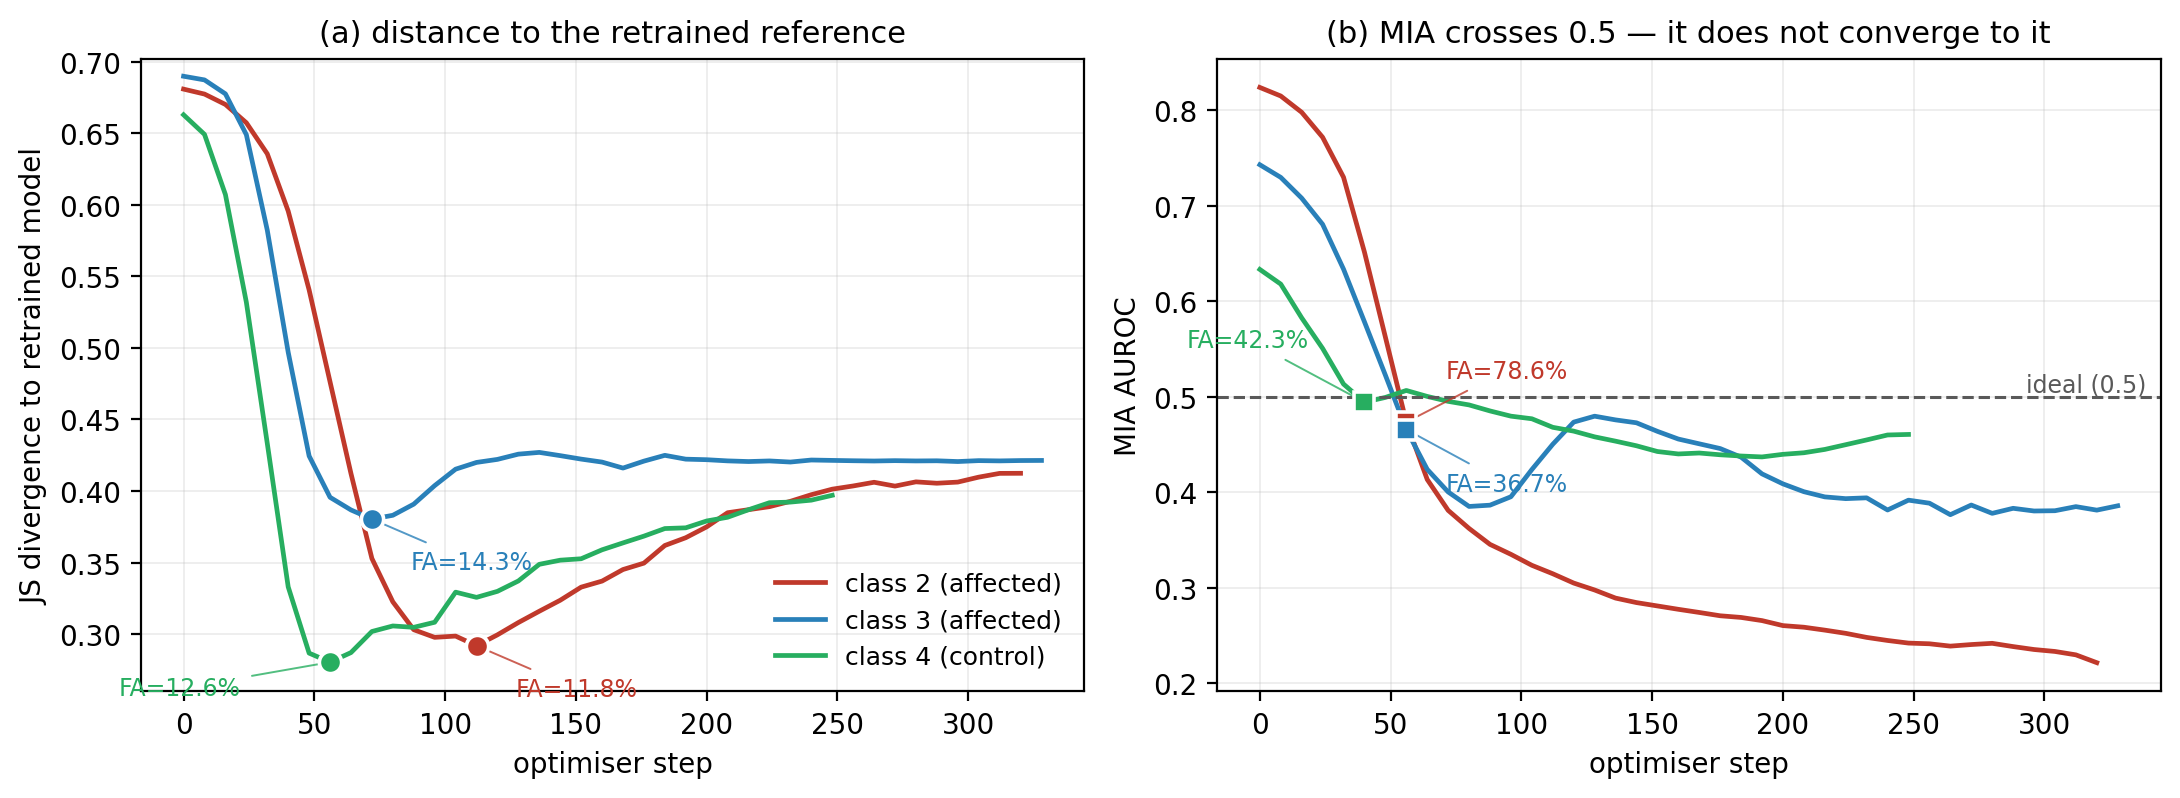
\includegraphics[width=\textwidth]{fig_trajectory.png}
\caption{\textbf{Unlearning overshoots the model it is trying to imitate, and
MIA cannot detect it.} \textbf{(a)}~Jensen--Shannon divergence to a
retrained-from-scratch reference along the unlearning trajectory. The curve is
U-shaped: the model first moves toward the reference, attains a minimum, then
moves away. Markers give the minimum, annotated with the forget accuracy there
($11.8$--$14.3\%$)---\emph{above} the $11.1\%$ chance level, whereas dual
stopping halts at ${\approx}7\%$. \textbf{(b)}~MIA AUROC on the same axis. It
sweeps \emph{through} the ideal $0.5$ rather than converging to it, so
$|\mathrm{MIA}-0.5|$ is minimised at the crossing. On class~2 that crossing
occurs while the model still classifies $78.6\%$ of the forget set
correctly.}
\label{fig:trajectory}
\end{figure}

\paragraph{The minimum is interior, and the current rule is past it.}
Divergence to the reference falls from $0.66$--$0.69$ at initialisation to
$0.28$--$0.38$, then rises again to $0.40$--$0.42$. So unlearning genuinely
moves the model toward a retrained one before moving away: over-forgetting is
not a metric artefact but a real overshoot in function space. The minimum lies
at $\mathrm{FA} = 11.8\%$, $14.3\%$ and $12.6\%$ for the three classes, while
dual stopping halts at ${\approx}7\%$ (\S\ref{sec:overforget}) --- past the
optimum in every case. Stopping at the minimum instead is close to free: test
accuracy changes by $-0.06$, $-0.03$ and $+0.79$pp and retain accuracy by
$+0.06$, $+0.36$ and $+0.08$pp. On the same trajectory it reduces divergence by
$0.016$, $0.003$ and $0.007$, and reduces $|\mathrm{MIA}-0.5|$ by $0.017$ and
$0.015$ on the two affected classes while moving the control by $+0.006$. This
is the pattern the criterion of \S\ref{sec:overforget} failed to produce:
the affected classes improve and the control stays put.

\paragraph{But the optimum is shallow, so we do not propose a numeric target.}
The three minima fall within $2.5$pp of one another in forget accuracy, which
invites the conclusion that ``stop at $\mathrm{FA}\approx 13\%$'' is a
deployable rule. The basin does not support that reading. Taking every
checkpoint within $5\%$ of the minimum divergence, the corresponding forget
accuracy spans $10.2$--$26.3\%$, $3.5$--$36.7\%$ and $6.9$--$21.9\%$ on the
three classes---$3.5$--$36.7\%$ overall. The agreement between the three
\emph{argmin} values is therefore largely a coincidence of where the snapshots
happened to land, and a single tuned number would not transfer. What the data
does support is directional and, we think, more useful: the optimum sits
\emph{above} the chance level, and a rule that drives forget accuracy to or
below chance is on the wrong side of it.

\paragraph{$|\mathrm{MIA}-0.5|$ is not an optimisation target.}
Panel~(b) is the more consequential finding. MIA AUROC does not converge to
$0.5$; it \emph{passes through} it, falling from $0.82$, $0.74$ and $0.63$ at
initialisation to $0.22$, $0.39$ and $0.46$ at the end. Consequently
$|\mathrm{MIA}-0.5|$ is minimised wherever the trajectory happens to cross,
which carries no information about unlearning quality. On class~2 the crossing
occurs at $\mathrm{FA} = 78.6\%$: a model that has barely forgotten anything
attains a \emph{perfect} MIA score. The two criteria also disagree about where
to stop, and in opposite directions---the divergence minimum and the MIA
minimum are $56$ steps apart on class~2, $56$ steps apart the other way on
class~3, and $8$ steps apart on class~4.

This sharpens the observation of \S\ref{sec:experiments} that a pre-unlearning
model already scores MIA $=0.533$. That was a single point; here we see the
whole path, and it shows that MIA $\approx 0.5$ is attainable at almost any
stage of unlearning, including stages with no meaningful forgetting at all.
Reporting MIA alongside forget accuracy is therefore not merely advisable but
necessary, and \emph{optimising} $|\mathrm{MIA}-0.5|$---which a practitioner
reading ``ideal $=0.5$'' might reasonably attempt---selects an arbitrary point
on the trajectory.

\paragraph{What remains unresolved.}
Stopping at the divergence minimum reduces over-forgetting without eliminating
it: class~2 still attains MIA $=0.315$ there, far from $0.5$. Nor do we have a
deployable rule, since locating the minimum requires the retrained reference
that unlearning exists to avoid, and the basin is too flat for a fixed forget
accuracy to stand in for it. We report the diagnosis---the stopping rule halts
on the wrong side of a real optimum---and leave a practical criterion open.
Whether the effect holds beyond the three PathMNIST classes measured here is
also untested; the experiment costs one unlearning run plus one retrained
reference per class.

% ============================================================
\section{Limitations in Full}\label{app:limitations}

\paragraph{Compute scales with classes and with data scarcity, and we cannot
predict it.} At \rev{its 15-epoch cap} \ours{} leaves STL-10 at
FA~$=75.7\%$, and an earlier version of this paper reported that as a failure
mode of the hard constraint on small forget sets. That diagnosis was wrong in
its conclusion though right about its cause. With 500 training images per class
the forget set yields only 4 mini-batches per epoch, ${\sim}60$ update steps in
total, and every step conflicts with the retain gradient---so progress per step
is small and the budget expires before forgetting completes. At 60 epochs, over
the same three seeds \rev{and with a per-step check and a $1\%$ target}, FA falls
to $1.73 \pm \rev{0.95}\%$ with RA~$=98.87\%$ \rev{(with the default $10\%$
target a single 60-epoch run stops at $9.2\%$)}. CIFAR-100
behaves the same way for a different reason: its per-class forget sets are small
because there are a hundred of them, and at 60 epochs its nine-class mean falls
from $4.07\%$ to $1.27 \pm \rev{0.39}\%$, bringing the $1\%$ chance level inside one
standard deviation. Neither constraint was infeasible; both runs were truncated.

What survives as a limitation is that we cannot say in advance how much budget a
new dataset needs. The binding resource is optimiser steps rather than epochs or
examples, and \ours{} offers no way to predict the requirement beyond monitoring
forget accuracy and continuing until the tolerance is met. A practitioner
deploying on an unfamiliar dataset should expect to discover the budget
empirically, and should treat a shared epoch count copied from another dataset
as a likely under-estimate.


\paragraph{Sample-level forgetting works, but at a cost the method cannot
control.} Every result in this paper removes a whole class. We tested the other
standard request type---forgetting a random subset of training points---on
CIFAR-10 at $1\%$ and $5\%$ of the training set, and report it as a scope limit
rather than a capability.

Two things go wrong, and they are different in kind. First, the forget objective
degenerates. \klr{} draws its power from the forget class being \emph{absent}
from the retain set, which drives $p_r$'s mass on that class to ${\sim}0$
(measured: $0.0002$); when the forget set is a random subset, the retain set
still covers every class and $p_r$ is uniform to three decimals
($0.100,0.100,\dots$). \klr{} therefore reduces exactly to
\texttt{kl\_uniform} in this regime, and the target carries no information about
\emph{which} points to forget. Second, dual stopping does not fire: the retain
budget is multiplicative on an initial retain loss of $0.0018$, so even at
$\alpha = 100$ both stopping-armed runs halted on the budget with forget accuracy
still at ${\sim}99.5\%$. A multiplicative budget is the wrong instrument against
a converged model; an absolute floor would be the right one.

Given a fixed 60-epoch budget and no stopping, forgetting does occur---forget
accuracy falls to $58.4\%$ at $1\%$ and $71.8\%$ at $5\%$---but
indiscriminately: retain accuracy falls from ${\sim}100\%$ to $73.2\%$ and test
accuracy to $71.9\%$, and forget accuracy ends \emph{below} test accuracy, which
is over-forgetting by the standard for this setting (a correctly unlearned point
should look like an unseen point of the same class, i.e.\ $\mathrm{FA}\approx
\mathrm{TA}$). The method has no mechanism to stop at that crossing.

The one clearly positive finding is the ablation. Removing the projection at
equal budget collapses the model completely: retain accuracy $14.2\%$ versus
$73.2\%$ with it, and test accuracy $17.1\%$ versus $71.9\%$---a $59$pp and
$55$pp difference respectively, far larger than the projection's effect in the
class-level ablation of Table~\ref{tab:ablation}. When forget and retain
gradients are drawn from the same distribution the conflict is near-total (the
projection fires on $100\%$ of steps), and the retain constraint is the only
thing keeping the model intact. The guarantee is therefore \emph{more}
load-bearing here, not less---which is why we regard sample-level forgetting as
a direction the constraint supports and the objective does not yet.

\paragraph{Mini-batch scope of the guarantee.} Theorem~\ref{thm:retain_safety}
bounds the \emph{sampled} retain objective---the quantity \ours{} projects
against---not the full-population retain loss. A population-exact per-step
guarantee would require controlling the gradient-variance term and is future
work.

\paragraph{The comparison with the closest prior work is structural, not
empirical.} Our separation from soft conflict-resolution methods
\citep{patel2025learning} rests on Theorem~\ref{thm:separation}(iv) and
Table~\ref{tab:properties}, both of which argue from the definition of the
update rule. We have not reimplemented that method and run it on our stack, so
we make no claim about how the two compare on accuracy, forgetting, or MIA. A
like-for-like empirical comparison is the most important piece of missing
evidence in this paper. Two related experiments are reported and should not be
mistaken for it: the projection-only ablation, isolating the projection from
\ours{}'s other three components (Table~\ref{tab:cifar10}), and the
projection-strength sweep, which interpolates our own update between a soft
penalty and the hard constraint (\S\ref{sec:strength}). Both test the mechanism;
neither runs the cited method.

\paragraph{Floating-point exactness.} The guarantee holds to float32 precision
(\S\ref{sec:alignment}); exact arithmetic would require float64 inner products.

\added{\paragraph{BatchNorm robustness is bought with compute, and is scoped.}
BN-robust \ours{} (\S\ref{sec:bn_robust}) survives the recalibration attack at
about seven times the wall-clock of the default configuration, because forgetting
that has to happen in the weights takes more steps. It was evaluated on two
datasets, CIFAR-10 (every class) and MNIST, and on base models that differ from
those behind the rest of the paper. It also defends only the normalisation
statistics: an attacker who modifies weights, as in the fine-tuning recovery
below, is outside what it changes.}

\paragraph{\rev{Sequential unlearning and fine-tuning recovery.}}
\rev{\emph{Sequential unlearning}: forgetting classes $0$, then $1$, then $2$
from each resulting checkpoint takes test accuracy $86.1 \to 76.8 \to 69.1$ and
retain accuracy $100.0 \to 89.7 \to 80.7$, with forget accuracy on the newest
class at most $2.7\%$. The decline is what forgetting does to these metrics,
not damage. TA counts every forgotten class's test images as errors, so fully
forgotten classes alone take it to $0.9$, $0.8$ and $0.7$ times the
retained-class accuracy (with the base model's $95.5\%$: $86.0$, $76.4$ and
$66.9\%$); RA is measured on a retain set that still contains the
earlier-forgotten classes, so fully forgotten classes take it to at most $8/9$
and $7/9$ ($88.9\%$ and $77.8\%$). The observed values sit at or above these
levels, so the retained classes are not damaged cumulatively. They sit above
them because earlier-forgotten classes partly return: an RA of $80.7\%$ requires
the two earlier classes to average at least $13\%$ training accuracy, above the
$10\%$ chance level. A sequential deployment should therefore re-check every
forgotten class after each request.} \emph{Fine-tuning recovery}: retraining the unlearned model on
$50$ forget-class samples raises forget accuracy from $1.9\%$ to $7.1\%$ after
five epochs and $51.3\%$ after ten---though by then the model is no longer
usable ($\mathrm{TA} = 34.6\%$, $\mathrm{RA} = 47.9\%$), so the attack recovers
the class only by destroying the model it attacks. \ours{} also does not provide
formal $(\varepsilon,\delta)$-DP guarantees.

\section{Per-Class Results}\label{app:perclass}

The main text reports per-dataset aggregates (Table~\ref{tab:cross}). Because a
mean over classes can conceal a method that succeeds on easy classes and fails on
hard ones, we report every class individually. Each row is the mean $\pm$
standard deviation over seeds $\{42,123,456\}$. CIFAR-100 per-class results
appear in the main text (Table~\ref{tab:cifar100}); the raw per-run CSVs for all
75 runs are released with the code.

\begin{figure}[t]
\centering
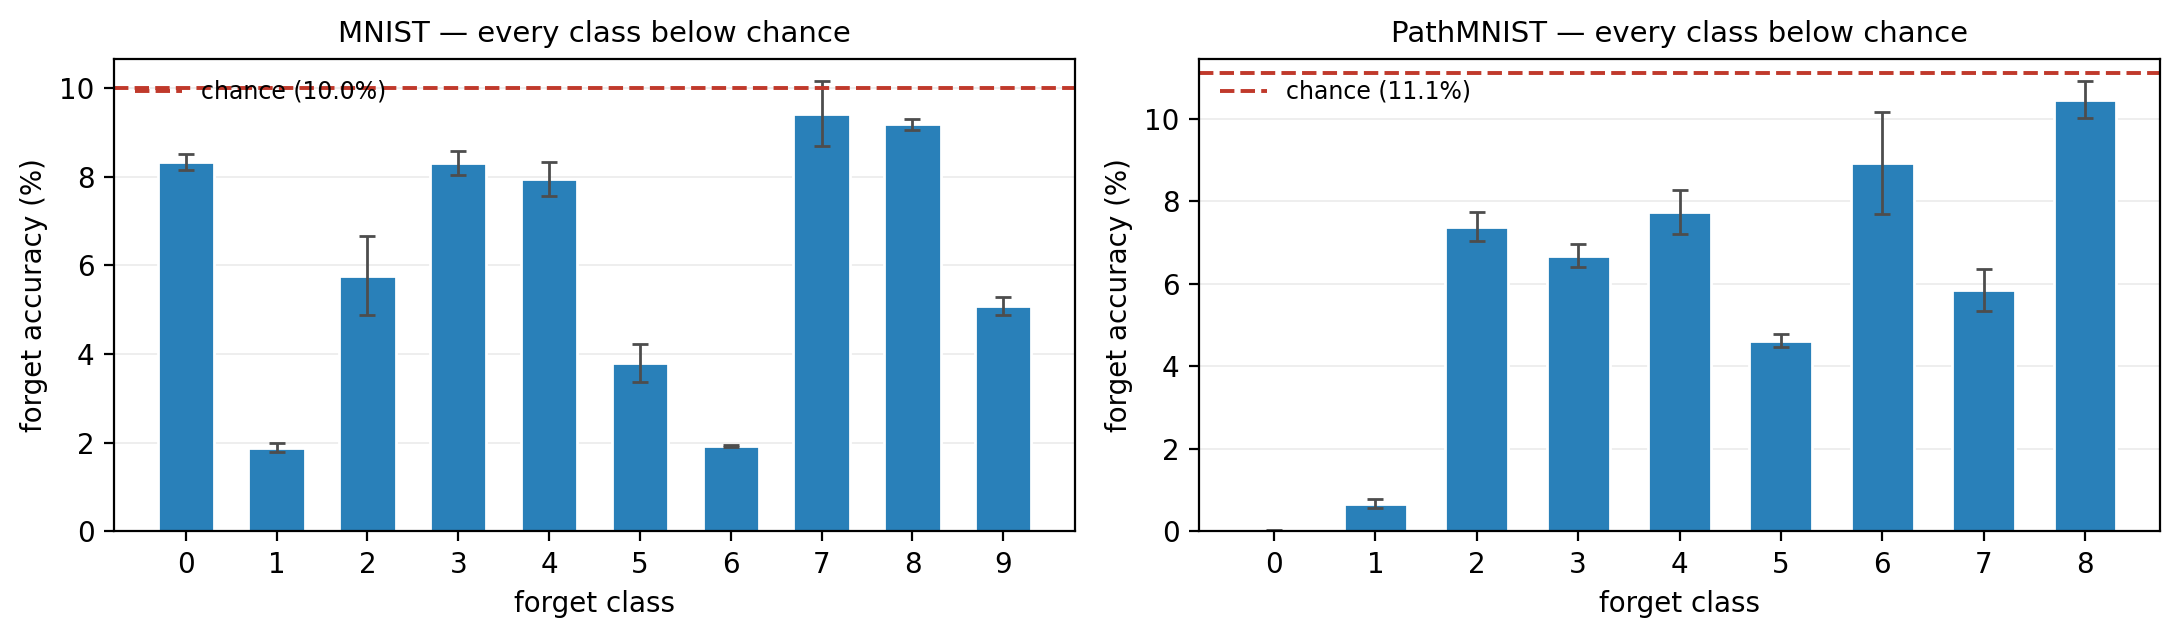
\includegraphics[width=\textwidth]{fig_perclass.png}
\caption{\textbf{Per-class forget accuracy} (mean $\pm$ std over three seeds).
Every MNIST and PathMNIST class individually falls below its chance level, so
the per-dataset means of Table~\ref{tab:cross} are not concealing a class that
fails.}
\label{fig:perclass}
\end{figure}

\subsection{MNIST (all 10 classes)}

Table~\ref{tab:app_mnist} gives all ten MNIST classes. Every class individually
falls below the $10\%$ chance level, with per-class mean FA ranging from
$1.89\%$ (class~1) to $9.42\%$ (class~7); the aggregate is therefore not
concealing a failure. Retain accuracy is essentially constant across classes
($99.42$--$99.54\%$), and MIA stays within $0.017$ of the ideal $0.5$ for every
class. Seed variance is small throughout (the largest FA standard deviation
across classes is $0.89$pp), indicating the procedure is stable rather than
seed-lucky.

\begin{table}[t]
\centering
\caption{\textbf{MNIST per-class forgetting} (mean $\pm$ std over 3 seeds).
Chance level is $10.0\%$; every class attains FA below it. TA is measured on the
full test set, so it necessarily drops by ${\sim}10$pp relative to the
$99\%$ base model once the forget class is correctly no longer recognised.}
\label{tab:app_mnist}
\begin{tabular}{@{}ccccc@{}}
\toprule
Forget class & TA (\%) & FA (\%)$\downarrow$ & RA (\%) & MIA \\
\midrule
0 & $90.26 \pm 0.05$ & $8.33 \pm 0.18$ & $99.42 \pm 0.00$ & $0.495 \pm 0.002$ \\
1 & $88.29 \pm 0.01$ & $1.89 \pm 0.09$ & $99.50 \pm 0.02$ & $0.512 \pm 0.001$ \\
2 & $89.68 \pm 0.07$ & $5.77 \pm 0.89$ & $99.51 \pm 0.01$ & $0.491 \pm 0.001$ \\
3 & $90.37 \pm 0.02$ & $8.31 \pm 0.27$ & $99.45 \pm 0.01$ & $0.483 \pm 0.001$ \\
4 & $90.22 \pm 0.01$ & $7.95 \pm 0.39$ & $99.43 \pm 0.02$ & $0.510 \pm 0.001$ \\
5 & $90.76 \pm 0.04$ & $3.80 \pm 0.43$ & $99.52 \pm 0.03$ & $0.499 \pm 0.001$ \\
6 & $90.08 \pm 0.02$ & $1.92 \pm 0.03$ & $99.50 \pm 0.02$ & $0.501 \pm 0.001$ \\
7 & $90.03 \pm 0.03$ & $9.42 \pm 0.74$ & $99.51 \pm 0.01$ & $0.490 \pm 0.000$ \\
8 & $90.36 \pm 0.03$ & $9.19 \pm 0.13$ & $99.50 \pm 0.02$ & $0.486 \pm 0.001$ \\
9 & $89.97 \pm 0.05$ & $5.09 \pm 0.21$ & $99.54 \pm 0.02$ & $0.503 \pm 0.000$ \\
\midrule
\textbf{Mean} & $\mathbf{90.00}$ & $\mathbf{6.17}$ & $\mathbf{99.49}$ & $\mathbf{0.497}$ \\
\bottomrule
\end{tabular}
\end{table}

\subsection{PathMNIST (all 9 classes)}

Table~\ref{tab:app_pathmnist} gives all nine PathMNIST tissue classes. Every
class again falls below the $11.1\%$ chance level, from $0.02\%$ (class~0) to
$10.46\%$ (class~8). Two observations deserve stating explicitly rather than
being averaged away.

First, the spread is far wider than on MNIST---per-class TA ranges from
$73.23\%$ to $89.28\%$---reflecting genuinely unequal class difficulty in
histopathology rather than instability: within-class seed variance remains small
(largest FA standard deviation $1.23$pp).

Second, and more importantly, \textbf{MIA AUROC is not uniformly near $0.5$}:
class~2 reaches $0.298$ and class~3 $0.388$, both well \emph{below} the ideal.
A value substantially below $0.5$ indicates that forget-class training samples
have become \emph{harder} to classify than forget-class test samples---the
signature of \emph{over}-forgetting, in which the unlearned model is
distinguishable from a retrained one in the opposite direction to a privacy
leak. It is detectable precisely because we report MIA per class and treat
distance from $0.5$ in either direction as a defect. We flag this as a real
limitation of the current stopping rule on PathMNIST: dual stopping targets FA,
which does not constrain how far past the retrained model's output statistics the
optimiser travels.

\begin{table}[t]
\centering
\caption{\textbf{PathMNIST per-class forgetting} (mean $\pm$ std over 3 seeds).
Chance level is $11.1\%$; every class attains FA below it. $^{\dagger}$Classes~2
and~3 show MIA well below the ideal $0.5$, indicating over-forgetting (see
text).}
\label{tab:app_pathmnist}
\begin{tabular}{@{}ccccc@{}}
\toprule
Forget class & TA (\%) & FA (\%)$\downarrow$ & RA (\%) & MIA \\
\midrule
0 & $73.23 \pm 0.06$ & $0.02 \pm 0.02$ & $99.01 \pm 0.01$ & $0.511 \pm 0.003$ \\
1 & $78.66 \pm 0.26$ & $0.68 \pm 0.12$ & $98.48 \pm 0.08$ & $0.473 \pm 0.003$ \\
2$^{\dagger}$ & $89.28 \pm 0.12$ & $7.38 \pm 0.35$ & $99.02 \pm 0.02$ & $0.298 \pm 0.003$ \\
3$^{\dagger}$ & $82.40 \pm 0.12$ & $6.68 \pm 0.28$ & $98.86 \pm 0.02$ & $0.388 \pm 0.005$ \\
4 & $78.04 \pm 0.08$ & $7.73 \pm 0.53$ & $98.95 \pm 0.03$ & $0.502 \pm 0.001$ \\
5 & $84.58 \pm 0.03$ & $4.62 \pm 0.15$ & $98.32 \pm 0.02$ & $0.548 \pm 0.001$ \\
6 & $78.58 \pm 0.25$ & $8.93 \pm 1.23$ & $98.77 \pm 0.06$ & $0.541 \pm 0.001$ \\
7 & $88.48 \pm 0.14$ & $5.85 \pm 0.50$ & $99.25 \pm 0.01$ & $0.562 \pm 0.001$ \\
8 & $75.36 \pm 0.04$ & $10.46 \pm 0.45$ & $99.28 \pm 0.03$ & $0.525 \pm 0.001$ \\
\midrule
\textbf{Mean} & $\mathbf{80.96}$ & $\mathbf{5.82}$ & $\mathbf{98.88}$ & $\mathbf{0.483}$ \\
\bottomrule
\end{tabular}
\end{table}

\paragraph{On the per-dataset MIA aggregate.}
The PathMNIST aggregate of $0.483 \pm 0.084$ in Table~\ref{tab:cross} is within
$0.017$ of ideal, but its standard deviation is an order of magnitude larger
than any other dataset's precisely because of classes~2 and~3. The aggregate is
accurate but uninformative here; this is a concrete instance of the more general
point of \S\ref{sec:experiments} that MIA must be read alongside FA, and
per-class rather than only in aggregate.

\begingroup\color{revised}% ---- new appendix subsection: added up to \endgroup
\subsection{BN-robust \ours{} on all ten CIFAR-10 classes}\label{app:bnrobust_perclass}

Table~\ref{tab:app_bnrobust} gives every CIFAR-10 class under the recalibration
attack of \S\ref{sec:bn_robust}, one seed per class (class~0 has three seeds in
Table~\ref{tab:bnrobust}). ``Pre'' and ``post'' are FA under test-time transforms
before and after \texttt{update\_bn} on the retain set. All runs share the
$93.97\%$ base of \S\ref{sec:bn_robust}. The calibrated runs here read the
stopping FA on the full retain set rather than the $10{,}240$-image subset; on
class~0 the two made identical stopping decisions (\S\ref{sec:bn_robust}).

\begin{table}[t]
\centering\color{revised}
\caption{\added{\textbf{BN-robust \ours{} per class} (CIFAR-10, seed~$42$). The
frozen-statistics configuration is recovered on every class. BN-robust is not,
under either stopping rule, and with calibrated stopping every class ships within
three standard errors of chance ($11.3\%$). Epochs ``$25{\to}22$'': the run
reached the cap and its best epoch was shipped.}}
\label{tab:app_bnrobust}
\small
\setlength{\tabcolsep}{4pt}
\begin{tabular}{@{}cccccccccc@{}}
\toprule
& \multicolumn{2}{c}{Frozen} & \multicolumn{2}{c}{BN-robust, naive}
& \multicolumn{5}{c}{BN-robust, calibrated} \\
\cmidrule(lr){2-3}\cmidrule(lr){4-5}\cmidrule(l){6-10}
Class & pre & post & pre & post & pre & post & epochs & TA & RA \\
\midrule
0 & $8.76$ & $99.22$ & $9.24$ & $9.28$ & $9.22$ & $9.24$ & 13 & $84.35$ & $95.60$ \\
1 & $2.40$ & $97.60$ & $10.66$ & $10.66$ & $6.66$ & $6.66$ & 8 & $84.56$ & $96.19$ \\
2 & $6.52$ & $98.30$ & $11.18$ & $11.16$ & $9.90$ & $9.92$ & 15 & $85.07$ & $95.27$ \\
3 & $4.78$ & $94.82$ & $11.30$ & $11.30$ & $10.00$ & $9.98$ & 16 & $85.92$ & $96.26$ \\
4 & $4.84$ & $97.34$ & $13.32$ & $13.34$ & $10.18$ & $10.16$ & $25{\to}22$ & $84.88$ & $94.74$ \\
5 & $7.28$ & $94.70$ & $8.78$ & $8.78$ & $9.40$ & $9.42$ & 12 & $84.52$ & $94.64$ \\
6 & $9.18$ & $99.14$ & $7.20$ & $7.20$ & $7.30$ & $7.30$ & 8 & $83.32$ & $94.41$ \\
7 & $3.38$ & $96.20$ & $11.36$ & $11.34$ & $9.12$ & $9.12$ & 10 & $84.49$ & $95.24$ \\
8 & $4.54$ & $99.26$ & $16.74$ & $16.68$ & $9.74$ & $9.68$ & 14 & $83.59$ & $94.67$ \\
9 & $2.52$ & $98.16$ & $15.44$ & $15.42$ & $8.92$ & $8.92$ & 11 & $83.84$ & $95.01$ \\
\midrule
Mean & $5.42$ & $97.47$ & $11.52$ & $11.52$ & $9.04$ & $9.04$ & --- & $84.45$ & $95.20$ \\
\bottomrule
\end{tabular}
\end{table}

\begin{figure}[t]
\centering\color{revised}
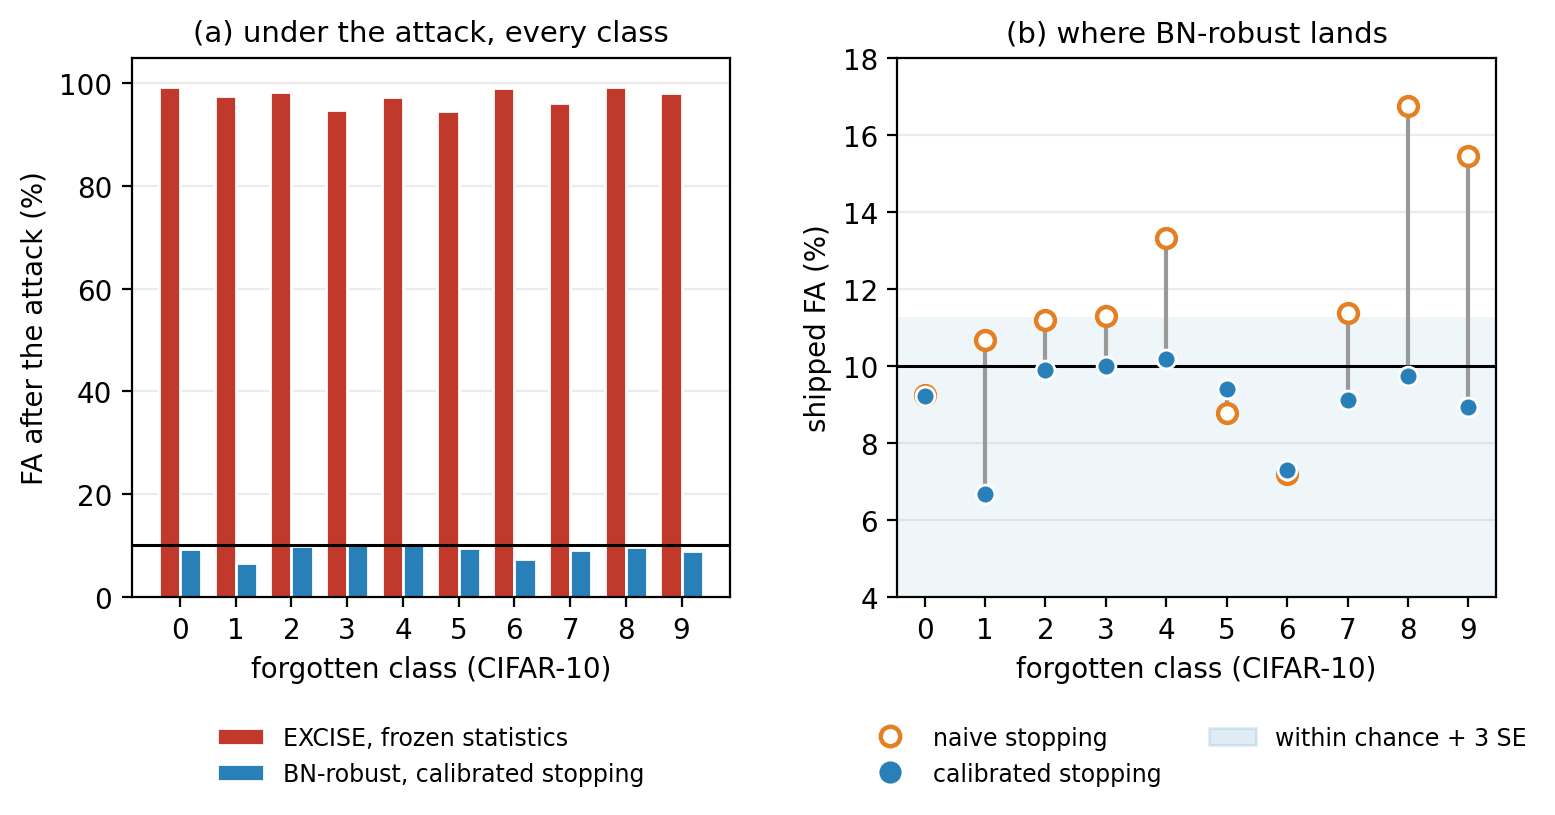
\includegraphics[width=\textwidth]{fig_bnrobust_perclass.png}
\caption{\added{\textbf{BN-robust on all ten CIFAR-10 classes} (seed~$42$; the data of
Table~\ref{tab:app_bnrobust}). (a)~Under the attack, the frozen-statistics
configuration is recovered on every class and BN-robust on none. (b)~Where
BN-robust ships: with naive stopping (open) five classes land above chance
$+\,3$\,SE; with calibrated stopping (filled), none do.}}
\label{fig:app_bnrobust}
\end{figure}
\endgroup% ---- end of the added appendix subsection

% ------------------------------------------------------------
\section{Hyperparameter Configuration}\label{app:hyper}

Table~\ref{tab:app_shared} lists the settings shared across all datasets and
Table~\ref{tab:app_perdataset} the per-dataset settings. All are released as YAML
configuration files; the reported runs use them unmodified.

\begin{table}[t]
\centering
\caption{\textbf{Shared hyperparameters} (identical for all six datasets). The
two components removed from \ours{} are listed explicitly with value $0$, since
they remain available as flags for the ablation of \S\ref{sec:ablation}.}
\label{tab:app_shared}
\begin{tabular}{@{}llll@{}}
\toprule
Symbol & Flag & Value & Role \\
\midrule
$\mu$ & \texttt{--momentum} & $0.9$ & momentum; projection applied \emph{after} accumulation \\
$c$ & \texttt{--max\_grad\_norm} & $1.0$ & clip on $d_t$, \emph{before} accumulation \\
$\lambda_{\mathrm{wd}}$ & \texttt{--weight\_decay} & $5\times10^{-4}$ & weight decay, applied inside $d_t$ \\
$T_{\mathrm{KD}}$ & \texttt{--temperature} & $4.0$ & distillation temperature \\
--- & \texttt{--forget\_objective} & \klr{} & KL toward retain-confusion $p_r$ \\
--- & \texttt{--batch\_size} & $128$ & forget and retain mini-batch size \\
--- & \texttt{--fa\_check\_freq} & $50$ & intra-epoch FA check interval (batches) \\
--- & \texttt{--seed} & $\{42,123,456\}$ & three seeds per task \\
\midrule
\multicolumn{4}{@{}l}{\emph{Removed components (retained as ablation flags only)}} \\
$\lambda$ & \texttt{--rep\_weight} & $0.0$ & representation erasure (removed) \\
$\gamma$ & \texttt{--forget\_gate} & $0.0$ & entropy gate (removed) \\
\bottomrule
\end{tabular}
\end{table}

\begin{table}[t]
\centering
\caption{\textbf{Per-dataset hyperparameters.} $K$ is the number of classes.
Note that the forget-accuracy target $\tau_F$ is set to the chance level
$100/K$ for every dataset---it is not tuned per dataset, but derived from the
task.}
\label{tab:app_perdataset}
\begin{tabular}{@{}lcccccc@{}}
\toprule
Dataset & $K$ & Epochs $T$ & $\eta$ & $\beta$ (KD) & $\alpha$ (retain budget) & $\tau_F = 100/K$ \\
\midrule
CIFAR-10  & 10  & 15 & $5\times10^{-4}$ & $2.0$ & $5.0$ & $10.0\%$ \\
CIFAR-100 & 100 & 20 & $5\times10^{-4}$ & $2.0$ & $5.0$ & $\phantom{0}1.0\%$ \\
MNIST     & 10  & 12 & $2\times10^{-4}$ & $3.0$ & $4.0$ & $10.0\%$ \\
SVHN      & 10  & 15 & $2\times10^{-4}$ & $3.0$ & $5.0$ & $10.0\%$ \\
STL-10    & 10  & 15 & $2\times10^{-4}$ & $5.0$ & $5.0$ & $10.0\%$ \\
PathMNIST & \phantom{0}9 & 12 & $2\times10^{-4}$ & $5.0$ & $4.0$ & $11.1\%$ \\
\bottomrule
\end{tabular}
\end{table}

\paragraph{Tuning effort.}
Only four quantities vary across datasets: the epoch cap $T$, the learning rate
$\eta$, the KD weight $\beta$, and the retain budget $\alpha$. The learning rate
takes one of two values ($5\times10^{-4}$ for the CIFAR datasets,
$2\times10^{-4}$ elsewhere), $\beta$ one of three, and $\alpha$ one of two. The
forget target $\tau_F$ is not tuned at all: it is fixed to the chance level
$100/K$ implied by the task. Notably, $\mu$, $c$, $\lambda_{\mathrm{wd}}$, and
$T_{\mathrm{KD}}$---the four quantities that enter the guarantee of
Theorem~\ref{thm:app_main}---are held constant across all six datasets, so the
bound $\tfrac12 L\eta^2(c/(1-\mu))^2$ varies across datasets only through
$\eta$ (and through the dataset-dependent smoothness constant $L$).

\paragraph{A note on defaults.}
The command-line default for \texttt{--max\_grad\_norm} in the released code is
$5.0$, whereas every configuration file sets $c=1.0$. Runs launched without
\texttt{--config} would therefore use a different clip threshold, and a
correspondingly weaker constant in
(\ref{eq:app_c}). All results in this paper use the configuration files. We note
this because the value of $c$ enters the guarantee directly, so it should not be
inherited silently from a default.

% ------------------------------------------------------------
\section{Distance to the Retrained Model: A Refuted Hypothesis}\label{app:d2r}

This appendix reports a negative result. We formed a hypothesis about why
\ours{} over-forgets on two PathMNIST classes, derived a deployable fix from it,
pre-committed to a falsifiable prediction, ran the experiment, and the
prediction did not hold. We report it in full because the experiment also
produced the diagnosis that we believe is correct, and because the refuted
hypothesis concerns \ours{}'s own forget objective.

\subsection{The defect, and the hypothesis}

Per-class reporting (Appendix~\ref{app:perclass}) showed that on PathMNIST
classes~2 and~3, MIA AUROC reaches $0.298$ and $0.388$---far \emph{below} the
ideal $0.5$. Forget accuracy is satisfied on both, so FA alone certifies these
runs as successes when they are not. A value below $0.5$ means forget-class
training samples have become \emph{harder} to classify than forget-class test
samples: the model is still distinguishable from a retrained one, in the
opposite direction to a privacy leak.

\rev{An earlier version of our forget-side condition (Eq.~\ref{eq:problem}) was
$\KL(p_\theta(x_f)\,\|\,p_r) \le \epsilon$}, a statement about
\emph{distributions}, but dual stopping (\S\ref{sec:stopping}) implements
\rev{$\mathrm{FA} \le \tau_F$}, a statement about \emph{argmax}. These are not
equivalent, and we hypothesised that the discrepancy was the cause: FA cannot
distinguish (a)~$p_\theta(x_f)$ having moved \emph{to} the distribution a
retrained model produces from (b)~having moved \emph{past} it, since both give
$\mathrm{FA}\approx 0$.

The hypothesised fix was to enforce the constraint as stated. Since $p_r$ is
computed from the \emph{original} model, this needs no retrained reference and
is deployable: stop on $\KL(p_\theta(x_f)\|p_r)$ rather than on FA. We reasoned
that this quantity is minimised at $p_\theta = p_r$ and rises on either side, so
a stop-when-it-stops-improving rule would halt at the minimum---exactly the
point FA cannot locate.

\paragraph{Prediction (pre-committed).} Replacing FA stopping with KL stopping
would, on the affected classes, (1)~reduce $|\mathrm{MIA}-0.5|$, (2)~reduce
Jensen--Shannon divergence to a retrained reference, and (3)~not materially
worsen FA or RA, while leaving an unaffected control class approximately
unchanged.

\subsection{Design}

We retrained reference models without the forget class for PathMNIST classes~2
and~3 (affected) and class~4 (control, MIA already $0.501$), keeping all $K$
output heads so that output distributions remain comparable, and training all
three identically for a fixed 30-epoch cosine schedule so that no reference is
better converged than another. Arm~A is \ours{} with FA stopping (the deployed
configuration); arm~B disables FA stopping and enables KL stopping. Oracle
metrics are computed against the references: JS divergence between output
distributions on the forget set (primary), top-1 agreement with the reference,
Fr\'echet distance between penultimate features, and MIA.

The control class is the load-bearing part of the design: a criterion that
merely stops earlier everywhere would improve the affected classes while also
perturbing the control, whereas a targeted fix should leave the control alone.

\subsection{Result: the prediction fails}

Table~\ref{tab:app_klstop} reports the outcome. Across three classes and four
metrics, arm~B is better on 2 comparisons and worse on 10. The primary oracle
metric---JS divergence to the retrained model---is \emph{worse in all three
classes}. The control class degrades on every metric, which is precisely the
signature that rules out a targeted fix. Only class~3 improves on
$|\mathrm{MIA}-0.5|$.

\begin{table}[t]
\centering
\caption{\textbf{KL stopping vs.\ FA stopping on PathMNIST}, measured against
retrained references. Arrows mark the direction of improvement. The prediction
was that the affected classes would improve and the control would not move;
neither held.}
\label{tab:app_klstop}
\begin{tabular}{@{}llccccc@{}}
\toprule
Class & Arm & $|\mathrm{MIA}{-}0.5|\downarrow$ & JS$\downarrow$ &
agree \%$\uparrow$ & Fr\'echet$\downarrow$ & $\KL$ to $p_r$ \\
\midrule
\multirow{2}{*}{2 (affected)}
 & FA stop & $0.205$ & $0.308$ & $45.4$ & $185.7$ & $0.957$ \\
 & KL stop & $0.268$ & $0.412$ & $23.5$ & $332.0$ & $0.052$ \\
\midrule
\multirow{2}{*}{3 (affected)}
 & FA stop & $0.115$ & $0.382$ & $31.2$ & $375.2$ & $0.805$ \\
 & KL stop & $\mathbf{0.068}$ & $0.421$ & $\mathbf{39.8}$ & $780.1$ & $0.002$ \\
\midrule
\multirow{2}{*}{4 (control)}
 & FA stop & $0.001$ & $0.286$ & $38.7$ & $141.1$ & $1.510$ \\
 & KL stop & $0.044$ & $0.399$ & $12.3$ & $297.7$ & $0.116$ \\
\bottomrule
\end{tabular}
\end{table}

\paragraph{The proxy is anti-correlated with the oracle.}
A proxy is only usable if it tracks the quantity it stands in for. Across the
six checkpoints, the rank correlation between $\KL(p_\theta\|p_r)$ and JS
divergence to the retrained model is $\rho = -1.00$ (Pearson $-0.94$): the
ordering is perfectly inverted. Driving the deployable proxy toward zero moves
the model monotonically \emph{away} from the retrained reference. This is the
opposite of the relationship the hypothesis required.

\subsection{Why it failed}

\paragraph{(i) The criterion never fired.}
In all three runs of arm~B the terminating condition was the retain-loss budget,
not the KL rule. The reason is visible in the logged trajectories:
$\KL(p_\theta(x_f)\|p_r)$ decreases essentially monotonically (class~2:
$5.53 \to 0.05$ over 8 checks with zero increases; class~4: $2.73 \to 0.07$,
zero increases; class~3: $2.06 \to 0.002$ over 20 checks with 4 small
increases). It never turns back up, so a stop-when-it-stops-improving rule
cannot trigger. The U-shape the hypothesis assumed does not exist over the
range the optimiser traverses.

This is also a limitation of the test, and we state it plainly: because the KL
rule never fired and FA stopping was disabled, arm~B is in effect \ours{}
\emph{without forget-side stopping} (FA reaches $0.0$ in all three runs), which
is closer to the $-$Stopping ablation than to a KL-stopped method. The
comparison in Table~\ref{tab:app_klstop} is therefore evidence against the
criterion \emph{as specified}, not a clean contrast between two stopping rules.

\paragraph{(ii) $p_r$ is a global average; a retrained model routes per-sample.}
$p_r$ is a single distribution, the retain-set average softmax, and it is the
same target for every forget sample. A retrained model does something different:
it routes each forget-class image to whichever surviving class that particular
image most resembles, giving an input-dependent output distribution. Matching
$p_r$ more closely therefore makes the model's predictions on forget data
unnaturally homogeneous across samples. The agreement column is the evidence:
as $\KL$ to $p_r$ falls by one to three orders of magnitude, top-1 agreement
with the reference \emph{collapses} on two of the three classes
($45.4 \to 23.5$ on class~2, $38.7 \to 12.3$ on class~4). If $p_r$ were the
right target, matching it better should have raised agreement. Class~3 moves the
other way ($31.2 \to 39.8$), so the effect is not universal.

\paragraph{Confound we cannot separate.}
$\KL$ to $p_r$ decreases with training time while JS to the reference increases
over the observed range, so the two are mechanically anti-correlated and the
$\rho = -1.00$ figure partly reflects run duration rather than target quality
alone. The agreement collapse is the part of the evidence that speaks to the
target itself, and it rests on two of three classes. We therefore claim the
criterion is refuted, and treat the mechanism as well-supported but not
established.

\subsection{What the experiment did establish}

\paragraph{The FA rule overshoots its own target.}
All three FA-stopped runs halt at $\mathrm{FA} \approx 7\%$ against a target of
$11.1\%$ (the chance level), overshooting by $3.9$--$4.2$pp, because the
intra-epoch FA check is evaluated only every 50 batches. The over-forgetting we
set out to explain is thus at least partly a \emph{granularity} defect in how
the existing criterion is enforced, not evidence that FA is the wrong quantity.

\paragraph{Less unlearning was better on every class.}
JS divergence to the retrained model is lower at the earlier stopping point in
all three classes. Over the range we observe, the model is still moving toward
the retrained reference when FA stopping halts it, and continues away from it
afterwards. Combined with the overshoot above, this points to stopping
\emph{earlier and more precisely} rather than to replacing the stopped quantity.

\paragraph{Consequence for the method.}
We draw a narrower conclusion about \klr{} than the original formulation
implies. As a forget-side \emph{direction}, $p_r$ is a better target than the
uniform distribution (\S\ref{sec:forget_obj}). As a \emph{target to be minimised
to zero}, it is actively harmful. \rev{Accordingly Eq.~\ref{eq:problem} states
the forget condition on forget accuracy and uses the divergence only as the
direction of the search}, and we do not claim $p_r$ is what a retrained model produces on forget
inputs---the measurements here show it is not.

\subsection{Open question}

Where JS divergence to the retrained model is minimised along the unlearning
trajectory remains unmeasured. Since JS is still falling when FA stopping fires
and rising afterwards, a minimum exists between the base model and the FA-stopped
point; locating it would establish whether a single FA level identifies it across
classes, which would make it deployable, or whether it varies per class, which
would not.
This question is answered in \S\ref{sec:trajectory}: the minimum is interior, lies above the chance level, and the current rule stops past it.

% ------------------------------------------------------------
\section{Ethical and Societal Considerations}\label{app:ethics}

\paragraph{Unlearning as evidence removal.}
A method that makes a model indistinguishable from one retrained without
specific data could be misused to destroy evidence that problematic data was
used for training. This is a dual-use property of the unlearning goal itself
rather than of \ours{} specifically, but \ours{} does make it concrete. Partial
mitigation is that \ours{} leaves an audit trail by construction: projection-rate
logs, the FA trajectory, and retain-loss budget history are all recorded per run,
so an auditor with access to the logs can establish that unlearning was applied
and to what extent. We note this is mitigation, not prevention---an adversary who
controls the logs controls the audit.

\paragraph{Selective fairness degradation.}
Class-level unlearning removes all samples of a class, which may correspond to a
demographic group. Crucially, the accuracy degradation we observe is
\emph{not} confined to the forgotten class: test accuracy falls beyond what the
removed class alone accounts for, and the per-class spread on PathMNIST
(Appendix~\ref{app:perclass}) shows the effect is uneven across classes.
Deployers should therefore monitor per-class accuracy before and after
unlearning rather than only aggregate accuracy, which can conceal a
disproportionate cost borne by one group.

\paragraph{Over-forgetting as a distinct harm.}
The PathMNIST finding (Appendix~\ref{app:perclass}) shows that a model can be
pushed \emph{past} the retrained reference. This matters ethically as well as
technically: such a model is still distinguishable from one trained without the
data, so a deletion request has not been faithfully honoured, yet every
FA-based check reports success. Compliance evidence resting on forget accuracy
alone would be misleading here.

\paragraph{Regulatory gap.}
Approximate unlearning methods, including \ours{}, do not satisfy formal
$(\varepsilon,\delta)$-differential-privacy certification. Whether
MIA AUROC~$\approx 0.5$ constitutes legally sufficient ``erasure'' under
instruments such as the GDPR right to erasure remains an open legal question on
which we take no position. The per-step guarantee of
Theorem~\ref{thm:retain_safety} is a statement about \emph{retain-side utility},
not a privacy certificate, and should not be presented as one.

% ------------------------------------------------------------
\section{Reproducibility}\label{app:repro}

\paragraph{Artefacts.}
Code, YAML configuration files, per-run summary CSVs for all 75 runs, and the
BatchNorm-recalibration diagnostic are released in the anonymised repository.
\todo{Insert the anonymised repository URL.}
The archived $\mu=0$ results underlying Table~\ref{tab:momentum} are released
alongside the main results, so the momentum ablation can be re-derived without
re-running it.

\paragraph{Environment.}
PyTorch $\ge 2.0$ with CUDA; ResNet-18 (11.7M parameters) throughout. Runs were
executed on a single GPU. Datasets download automatically except PathMNIST,
which is obtained through \texttt{medmnist}.

\paragraph{Implementation details that affect results.}
\begin{itemize}
\item Momentum and weight decay are applied \emph{manually} so that the
projection acts on the post-momentum update; the underlying \texttt{torch} SGD
object is configured with \texttt{momentum=0}, \texttt{weight\_decay=0} and acts
only as a plain step. Reading the optimiser construction alone is therefore
misleading---see \S\ref{sec:optimiser} and Appendix~\ref{app:setup}.
\item Clipping is applied to $d_t$ before momentum accumulation, and \emph{not}
to the final update. Reversing this changes the effective step size by a factor
$1/(1-\mu)$ (Proposition~\ref{prop:clip}).
\item The projected update is rescaled to the pre-projection norm.
\item BatchNorm layers are set to \texttt{eval()} immediately after the model is
set to \texttt{train()}, so running statistics are frozen during unlearning.
\added{BN-robust \ours{} (\S\ref{sec:bn_robust}) instead recomputes them from
$512$ retain images before every step (\texttt{--bn\_robust exact
--bn\_recal\_samples 512}) and on the full retain set under test-time transforms
after the last step. It reads the stopping forget accuracy under statistics
recomputed from $10{,}240$ retain images (\texttt{--bn\_calibrated\_stop
--bn\_stop\_recal\_samples 10240}), ships the best epoch when the target is not
met (\texttt{--restore\_best\_epoch}), and uses an epoch cap of $25$.}
\item The retain-confusion distribution $p_r$ is precomputed once from the frozen
original model.
\item Forward hooks are registered on \texttt{layer3}, \texttt{layer4}, and
\texttt{avgpool} for feature-level diagnostics.
\item Configuration files set $c=1.0$; the CLI default is $5.0$ (see above).
\item All baselines are re-run within the same codebase under a unified MIA
protocol, rather than quoted from their source papers.
\end{itemize}

\paragraph{Determinism and seeds.}
Every 10-class task is run with seeds $\{42,123,456\}$ and reported as
mean~$\pm$~std; CIFAR-100 uses a single seed per class. Seed variance is small
(Appendix~\ref{app:perclass}). As an internal consistency check, the two
ablation variants that are no-ops under the shipped configuration
(\texttt{--rep\_weight 0}, \texttt{--forget\_gate 0}, both already $0$) produce
byte-identical metrics, confirming both that the runs are deterministic given a
seed and that those components are genuinely inactive.

\paragraph{Known reproduction caveats.}
The floating-point exactness of the guarantee is precision-dependent
(Remark~\ref{rem:float}): reference implementations should accumulate the
projection inner products in float64. Wall-clock timings depend on the GPU and
on how early dual stopping fires, so step counts rather than seconds are the
portable quantity.

\end{document}
"
\ifdefined\finalversion
  \definecolor{revised}{RGB}{0,0,0}
  \definecolor{revisedB}{RGB}{0,0,0}
\else
  \ifdefined\showpreviousround
    \definecolor{revised}{RGB}{204,85,0}
  \else
    \definecolor{revised}{RGB}{0,0,0}
  \fi
  \definecolor{revisedB}{RGB}{0,84,180}
\fi
\newcommand{\added}[1]{{\color{revised}#1}}
\newcommand{\rev}[1]{{\color{revisedB}#1}}

\newtheorem{theorem}{Theorem}
\newtheorem{proposition}{Proposition}
\newtheorem{lemma}{Lemma}
\newtheorem{corollary}{Corollary}
\theoremstyle{remark}
\newtheorem{remark}{Remark}
\theoremstyle{plain}

\title{Provably Retain-Safe Machine Unlearning\\ via Gradient Projection}

\author{\name Anonymous \email anonymous@example.com \\
        \addr Anonymous Institution}

\begin{document}
\maketitle
\suppressfloats[t]% Figure 1 goes to the top of page 2, not above the title

\begin{abstract}
Machine unlearning must remove a class's influence from a trained network
without damaging what the network should keep---a forget--retain trade-off dual
to the stability--plasticity trade-off of continual learning. We adapt A-GEM's
gradient projection so that every unlearning step lies in the retain-safe
half-space $\{u : \langle u,\gr\rangle \ge 0\}$, and apply it to the
post-momentum update the optimiser actually takes rather than to the raw
gradient. The resulting per-step retain-safety guarantee is exact for the
deployed optimiser; removing momentum to simplify the analysis instead
\rev{leaves forget accuracy far above chance on five of six datasets}. \ours{}
pairs the projected update with a
retain-confusion forget objective and stopping rules derived from explicit
tolerances. Across six datasets and 31 class-level forgetting tasks with
ResNet-18 it drives forget accuracy to \rev{within sampling error of} the chance
level on all six (two at a longer epoch budget), with retain accuracy at or above
$97.2\%$ on the 10-class datasets, and step-level logs \rev{of a CIFAR-10 run}
confirm the constraint at every step. \rev{On BatchNorm backbones, forgetting
learned against frozen normalisation statistics is undone by recomputing
them---as concurrent work finds for six of nine prior methods. A variant that
keeps the statistics consistent with the weights forgets to chance on every
CIFAR-10 class and on MNIST and survives that attack, including when the
attacker chooses the recalibration data.} We also find that the conventional
membership-inference
target of $0.5$ is the wrong reference point: a retrained model scores $0.69$ on
CIFAR-10, and between $0.31$ and $0.70$ across PathMNIST classes.
\end{abstract}

% ============================================================
\section{Introduction}\label{sec:intro}

Trained models increasingly need to demonstrably \emph{forget} specific
data---to honour deletion requests, revoke expired licences, or remove poisoned
samples. Retraining without the data does this exactly but is costly
(\rev{under an hour} for a ResNet-18 on CIFAR-10 on one A100, days for production
models), so \emph{machine unlearning} (MU) asks how to modify a trained model so
that it behaves as if the data had never been seen. The hard part is not erasing
the data's influence but doing so \emph{without collateral damage}: what must be
erased and what must be kept live in the same weights, so any step that degrades
the forgotten data also perturbs everything else.

\begin{figure}[t]
\centering\color{revisedB}
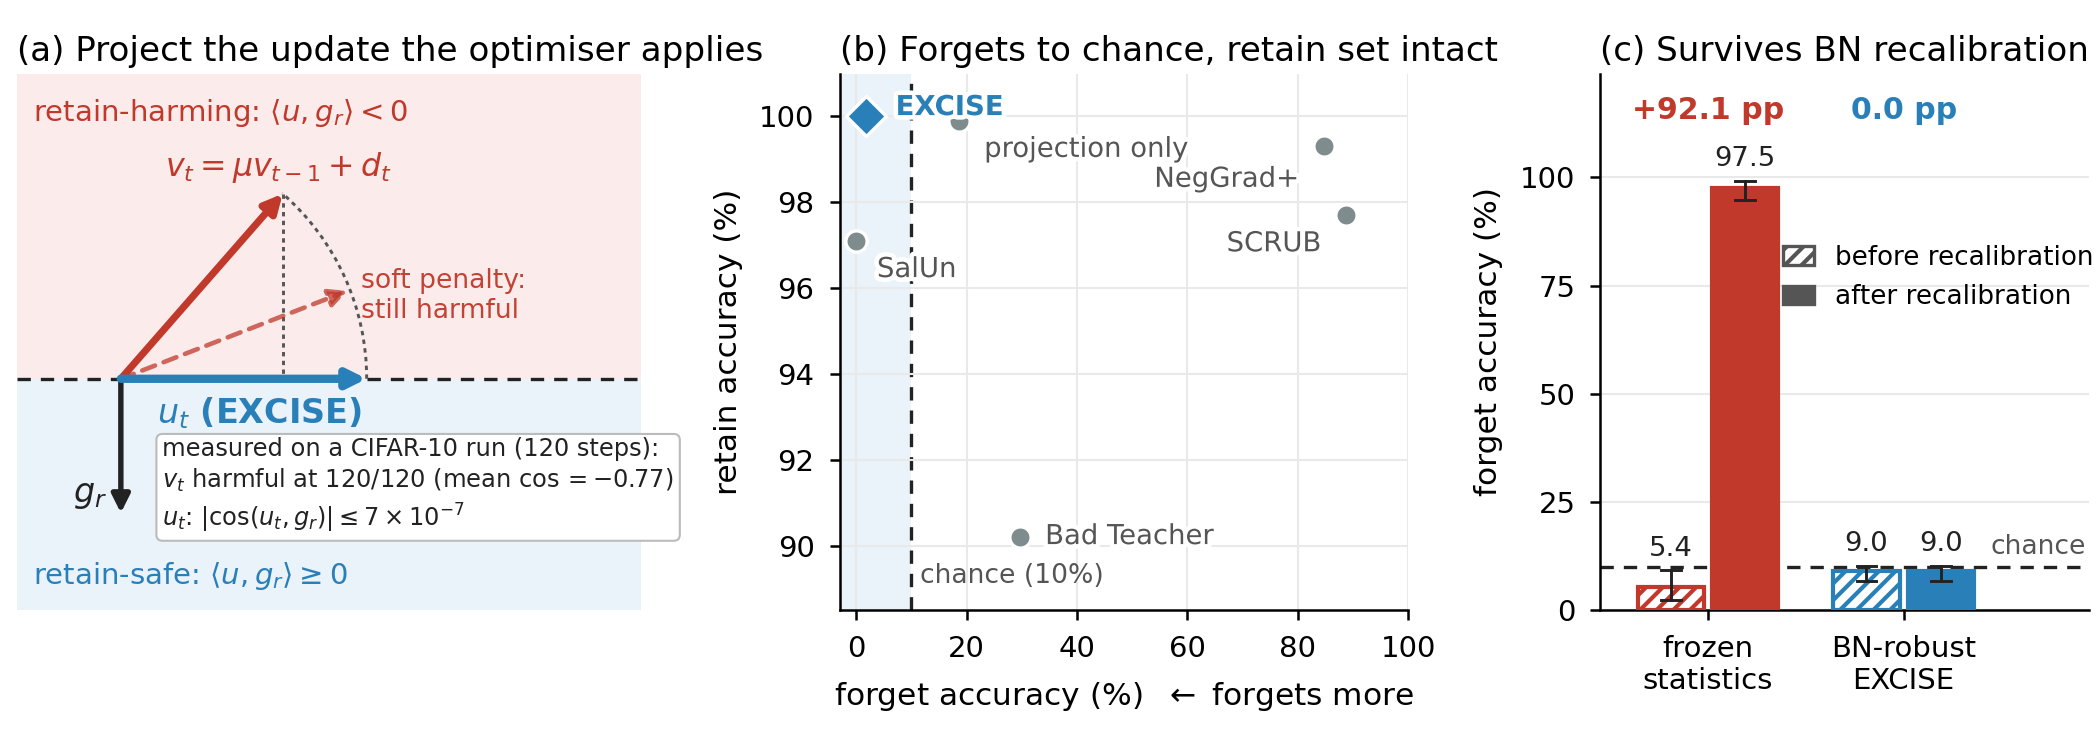
\includegraphics[width=\textwidth]{fig_teaser.png}
\caption{\rev{\textbf{\ours{} in one picture.} \textbf{(a)}~With momentum, the
update the optimiser applies is the accumulated $v_t$, and in unlearning it
points into the retain-harming half-space at every step. \ours{} projects $v_t$
onto the boundary and restores its length, so the applied $u_t$ cannot increase
the sampled retain loss to first order (Theorem~\ref{thm:retain_safety}); a
soft penalty only tilts the step, which stays harmful
(Theorem~\ref{thm:separation}). The boxed numbers are measured
(Figure~\ref{fig:guarantee}). \textbf{(b)}~On CIFAR-10 class~0, \ours{} is the
only method in Table~\ref{tab:cifar10} that forgets to chance with the retain
set intact. \textbf{(c)}~With frozen BatchNorm statistics, recomputing them on
retained data undoes the forgetting on every CIFAR-10 class; BN-robust \ours{}
does not move. Bars are means over the ten classes and whiskers their range
(Table~\ref{tab:app_bnrobust}).}}
\label{fig:teaser}
\end{figure}

\paragraph{The mirror image in continual learning.}
Continual learning (CL) faces the same problem with the sign reversed: learn a
new task while protecting old ones. \rev{One of its most direct answers} is not
a penalty but a \emph{constraint on the update}. A-GEM \citep{chaudhry2019agem} projects any
update $v$ with $\langle v, g_{\text{old}}\rangle < 0$ onto the half-space
$\{u : \langle u, g_{\text{old}}\rangle \ge 0\}$, so a step that would increase
old-task loss to first order is never taken. Unlearning lacks exactly this
guarantee: \rev{most} existing methods control retain damage with weighted
objectives, saliency masks or alternating updates (\S\ref{sec:related}), which
\rev{discourage retain-harming steps rather than exclude them}. We treat the retain set as CL's ``old task'' and
adopt the half-space constraint as the update rule for unlearning. The duality
has been noted before \citep{kurmanji2023unbounded,nguyen2020variational}, and
the forget--retain conflict has been targeted by a soft regulariser
\citep{patel2025learning}\added{ and by projecting updates away from a retain
gradient subspace \citep{hoang2024learn}}; what has not been done\rev{, to our
knowledge,} is to enforce the half-space constraint \rev{against the current
retain gradient}, at every step, on the vector the optimiser applies.

\paragraph{What it takes.}
Three design decisions \rev{complete the method}. \emph{Project the update, not
the gradient}: with momentum, the applied vector is the accumulated update, and
projecting the gradient certifies nothing about it
(Proposition~\ref{prop:counter}). Removing momentum would make the analysis
exact but \rev{leaves forget accuracy far above chance on five of six datasets}
(\S\ref{sec:momentum_ablation}), so we project the post-momentum update and make
the guarantee hold for the optimiser that runs. \emph{Push the forgotten class
toward the model's own retain-confusion distribution}, rather than the uniform
distribution no trained model produces\rev{; at equal test accuracy it forgets
further than gradient ascent and slightly further than a uniform target}
(\S\ref{sec:forget_obj}). \emph{Stop on explicit tolerances} for retain loss and
forget accuracy rather than on an epoch count (\S\ref{sec:stopping}).

\paragraph{Forgetting that survives the attack.}
A fourth issue came from the experiments. Forget batches contain a single
class and would corrupt BatchNorm running statistics, so the method freezes them
during unlearning---and the weights then learn to forget \emph{relative to}
statistics an attacker can replace: recomputing them on retained data restores
forget accuracy from ${\sim}1\%$ to ${\sim}100\%$ without changing a weight
(\S\ref{sec:bn_results}). \rev{The attack reaches beyond us. Concurrent work
\citep{kalani2026batchnorm} applies it to nine prior methods and recovers the
forgotten class for six of them; of the other three, gradient ascent forgets
only by destroying the model ($57\%$ retain accuracy), GA+FT does not forget
($68\%$ forget accuracy), and SCRUB keeps its forgetting at $88\%$ retain
accuracy. Whether a method survives depends less on the method than on how its
statistics are handled during unlearning: in \citet{kalani2026batchnorm},
mixing at least a quarter of retained data into SalUn's unlearning batches
removes its recovery, and our own reproductions of SalUn and Bad Teacher, which
end every epoch with a pass over retained data that recomputes the statistics,
are not recovered at all. BN-robust \ours{} makes survival a property of the
method rather than of how it is run: it keeps the statistics consistent with the
weights throughout unlearning, forgets to chance on every CIFAR-10 class and on
MNIST, survives the attack in every case we tried---including when the attacker
chooses the recalibration data---and keeps the per-step guarantee
(\S\ref{sec:bn_robust}). To our knowledge it is the only unlearning method for
BatchNorm ResNets whose survival has been verified on every class of a benchmark
and against attacker-chosen recalibration data, which we take to make it the
state of the art for this setting, pending a like-for-like run of the prior
methods under the same base and attack (\S\ref{sec:limitations}).}

\paragraph{Contributions.}
\textbf{(1)}~A constrained formulation of class unlearning
(Eq.~\ref{eq:problem}) \rev{that assigns each mechanism of the algorithm to the
condition it enforces}.
\textbf{(2)}~\ours{}: A-GEM projection as the \emph{update rule} of unlearning,
applied to the post-momentum update, with clipping before accumulation and
magnitude-preserving projection. \textbf{(3)}~An exact per-step retain-safety
theorem for that optimiser, a separation theorem showing that gradient ascent,
SCRUB, SalUn and soft conflict penalties admit retain-harming steps, and
\rev{tests of both theorems on real runs}. \textbf{(4)}~\rev{A
BatchNorm-recalibration failure mode of \ours{} and a fix that keeps BatchNorm,
verified on every CIFAR-10 class, on MNIST and against attacker-chosen
recalibration data.} We also show that the conventional MIA target of $0.5$ is
the wrong reference point for class unlearning (\rev{\S\ref{sec:mia_main}}).
\rev{Table~\ref{tab:claims} maps every claim to the experiment that tests it.}

% ============================================================
\section{Related Work}\label{sec:related}

\emph{Exact} unlearning retrains on shards \citep{bourtoule2021sisa} or certifies
removal for convex models \citep{guo2020certified}. \emph{Approximate} methods
modify the trained model: gradient ascent and NegGrad+ \citep{thudi2022unrolling}
maximise forget loss, the latter with a weighted retain term; SalUn
\citep{fan2024salun} confines random-label updates to a saliency mask; Fisher
methods and SSD \citep{golatkar2020eternal,foster2024ssd} dampen parameters by
estimated importance; Bad Teacher \citep{chundawat2023badteacher} and SCRUB
\citep{kurmanji2023unbounded} use distillation, SCRUB alternating forget and
retain steps. Each balances forgetting against retain damage through a weight, a
mask or a schedule, so retain damage is discouraged rather than excluded
(Theorem~\ref{thm:separation}). Closest to us are methods that address the
forget--retain gradient conflict directly: \citet{patel2025learning} with a soft
regulariser that rewards positive alignment, and \added{\citet{hoang2024learn}
by stepping orthogonally to a gradient subspace estimated for the retained
data}. \ours{} instead imposes A-GEM's half-space constraint
\citep{chaudhry2019agem} against the current retain gradient at every step, on
the post-momentum update the optimiser applies, which is what makes its guarantee
exact for the deployed optimiser. Table~\ref{tab:properties} summarises the structural
difference; Appendix~\ref{app:related} gives the full comparison. \rev{On the
evaluation side, \citet{kalani2026batchnorm} show that recomputing BatchNorm
statistics recovers the forgotten class for six of nine prior methods;
\S\ref{sec:bn_results} applies the same attack to \ours{}.}

\begin{table}[t]
\centering
\caption{\textbf{Structural comparison of update rules.} \cmark~= holds by
construction, \pmark~= partial or hyperparameter-dependent, \xmark~= not
provided. Entries are properties of each method's \emph{definition}, not
measured quantities; an empirical comparison against
\citet{patel2025learning} is future work (\S\ref{sec:limitations}).
P\&Q = \citet{patel2025learning}; \rev{PGU = \citet{hoang2024learn}, whose
projection removes the update's component in a retain subspace estimated before
unlearning and truncated at an energy threshold, so its protection is
approximate and not stated against the current retain gradient.}
$^\dagger$\ours{} takes an explicit tolerance and honours it across a $29$pp
range, but only when the stopping rule is evaluated per step: at a 50-batch
check granularity, targets from $5\%$ to $30\%$ collapse onto the same operating
point (\S\ref{sec:further}, Table~\ref{tab:sweeps}).}
\label{tab:properties}
\small
\begin{tabular}{@{}lccccccc@{}}
\toprule
\textbf{Property} & \textbf{GA} & \textbf{SalUn} & \textbf{SCRUB} &
\textbf{NG+} & \textbf{P\&Q} & \rev{\textbf{PGU}} & \textbf{\ours{}} \\
\midrule
Addresses forget--retain gradient conflict & \xmark & \xmark & \pmark & \pmark & \cmark & \cmark & \cmark \\
Conflict handled as a constraint, not a penalty & \xmark & \xmark & \xmark & \xmark & \xmark & \cmark & \cmark \\
Retain-harming steps are unreachable & \xmark & \xmark & \xmark & \xmark & \xmark & \pmark & \cmark \\
Per-step retain-safety guarantee & \xmark & \xmark & \xmark & \xmark & \xmark & \pmark & \cmark \\
Explicit forgetting tolerance & \xmark & \xmark & \pmark & \pmark & \pmark & \pmark & \cmark$^\dagger$ \\
Guarantee holds for the optimiser actually run & \xmark & \xmark & \xmark & \xmark & \xmark & \pmark & \cmark \\
\bottomrule
\end{tabular}
\end{table}

% ============================================================
\section{Problem Formulation}\label{sec:problem}

Let $f_\theta$ be a trained $K$-class classifier with weights $\theta_0$,
$\sigma$ the softmax, and $p_\theta(x) = \sigma(f_\theta(x))$. The training set
splits into a forget set $\Df$ and a retain set $\Dr$. We evaluate with test
accuracy (TA, held-out data), forget accuracy (FA, on $\Df$; a fully unlearned
model reaches at most the chance level $100/K\%$), retain accuracy (RA, on
$\Dr$), and the AUROC of a membership-inference attack (MIA) between forget-class
training and test samples. The \emph{retain-confusion distribution} is the base
model's average prediction on retained data,
\begin{equation}\label{eq:retain_confuse}
p_r = \frac{1}{|\Dr|}\sum_{x \in \Dr} \sigma(f_{\theta_0}(x)),
\end{equation}
and we pose unlearning as \rev{a constrained search: find
\begin{equation}\label{eq:problem}
\theta^\star \in \big\{\theta :\;
\mathrm{FA}(\theta;\Df) \le \tau_F,\;\;
\CE(\theta;\Dr) \le \alpha\,\CE(\theta_0;\Dr),\;\;
\|\theta - \theta_0\| \le R \big\},
\end{equation}
where $\tau_F$ is a forget-accuracy target (the chance level by default),
$\alpha \ge 1$ a tolerance on the retain loss, and $R$ a trust radius. The first
two conditions say what it means to have forgotten without damage; the third
asks for a solution near the trained model, and the search path supplies it.
\ours{} starts at $\theta_0$, descends the forget objective
$\lossf = \mathbb{E}_{x_f}[\KL(p_\theta(x_f)\|p_r)]$ along directions that do
not increase the retain objective
$\lossr = \mathbb{E}_{(x,y)}[\CE(f_\theta(x),y)] + \beta\,\losskd$ to first
order, where $\beta$ weights a distillation anchor, and returns the first point
that meets the forget target. $\lossf$ supplies the direction, not the
destination: driving it to its minimum over-forgets (Appendix~\ref{app:d2r}).
Retain safety is imposed at two levels. At every step the projection of
\S\ref{sec:projection} keeps the applied update in
$\{u : \langle u,\gr\rangle \ge 0\}$, so the sampled retain objective cannot
increase to first order (Theorem~\ref{thm:retain_safety}); on the full retain
set, the stopping rule ends the search if the retain cross-entropy exceeds its
tolerance. The first level is a hard constraint rather than a penalty because a
Lagrangian relaxation would turn it back into the soft treatment whose feasible
set still contains retain-harming steps (Theorem~\ref{thm:separation}(iv)). The
trust region needs no mechanism of its own: every step has length at most
$\eta c/(1-\mu)$ (Theorem~\ref{thm:retain_safety}), so $N$ steps stay within
$R = N\eta c/(1-\mu)$. Table~\ref{tab:constraint_map}
(Appendix~\ref{app:method}) maps each condition to its mechanism.}

% ============================================================
\section{The \ours{} Algorithm}\label{sec:method}

Algorithm~\ref{alg:excise} gives the update. Each step computes a retain gradient
$\gr$ on a retain mini-batch (cross-entropy plus the distillation anchor) and a
forget gradient $\gf$ on a forget mini-batch.

\begin{algorithm}[t]
\caption{\ours{} unlearning (projected-momentum update)}\label{alg:excise}
\begin{algorithmic}[1]
\REQUIRE Trained model $\theta$, forget set $\Df$, retain set $\Dr$;
         lr $\eta$, momentum $\mu$, clip $c$, weight decay $\lambda_{\mathrm{wd}}$;
         \rev{targets $\tau_F$, $\alpha$; check interval $m$}
\ENSURE Unlearned model $\theta^*$
\STATE $\theta_{\text{orig}} \leftarrow \text{freeze}(\text{copy}(\theta))$;\quad
       set all BatchNorm layers to \texttt{eval} mode
\STATE $p_r \leftarrow \frac{1}{|\Dr|}\sum_{x \in \Dr}\sigma(\theta_{\text{orig}}(x))$
\STATE $L_0 \leftarrow \CE(\theta,\Dr)$;\quad $v \leftarrow 0$
\FOR{epoch $=1$ to $T$}
  \FOR{$(x_f,y_f)$ in $\Df$}
    \STATE Sample $(x_r,y_r)$ from $\Dr$
    \STATE $\gr \leftarrow \nabla_\theta[\CE(f_\theta(x_r),y_r) + \beta\losskd]$
    \STATE $\gf \leftarrow \nabla_\theta\lossf(\theta;x_f)$
    \STATE $d \leftarrow \mathrm{clip}_c\!\big(\gf + \lambda_{\mathrm{wd}}\theta\big)$
           \hfill\textit{// clip BEFORE accumulation}
    \STATE $v \leftarrow \mu v + d$
           \hfill\textit{// momentum}
    \IF{$\langle v, \gr\rangle < 0$}
      \STATE $u \leftarrow v - \frac{\langle v,\gr\rangle}{\|\gr\|^2}\gr$;\quad
             $u \leftarrow u\,\|v\|/\|u\|$
             \hfill\textit{// project the update, rescale}
    \ELSE
      \STATE $u \leftarrow v$
    \ENDIF
    \STATE $\theta \leftarrow \theta - \eta u$
    \IF{\rev{every $m$ steps:} $\mathrm{FA}(\theta,\Df) \le \tau_F$}
      \STATE \textbf{return} $\theta$ \hfill\textit{\rev{// forget target met}}
    \ENDIF
  \ENDFOR
  \IF{$\CE(\theta,\Dr) > \alpha L_0$}
    \STATE \textbf{return} $\theta$ \hfill\textit{\rev{// retain tolerance exceeded}}
  \ENDIF
\ENDFOR
\RETURN $\theta^* \leftarrow \theta$
\end{algorithmic}
\end{algorithm}

\subsection{Projection onto the Retain-Safe Half-Space}\label{sec:projection}

When a candidate update $v$ satisfies $\langle v,\gr\rangle < 0$, moving along it
would increase the retain loss to first order, and we replace it by its
projection
\begin{equation}\label{eq:projection}
\Pi_{\gr}(v) = v - \frac{\langle v,\gr\rangle}{\|\gr\|^2}\,\gr,
\qquad \langle \Pi_{\gr}(v),\gr\rangle = 0 .
\end{equation}
This is A-GEM's operator: the minimum-norm correction that restores
feasibility, at the cost of one extra backward pass. What changes is its role.
In A-GEM it occasionally corrects a process whose objective already points the
right way; in unlearning, erasing a class and keeping the rest are directly
opposed, and the projection fires at \rev{$96$--$100\%$ of steps in every \ours{}
run we logged} (\S\ref{sec:guarantee_measured}). It becomes the optimiser's defining step rather
than a safeguard, which has three consequences for how it must be applied.

\subsection{Which Vector to Project}\label{sec:optimiser}

\emph{(i) Project the update, not the gradient.} \ours{} uses SGD with momentum
$\mu$, weight decay and clipping $c$. The vector applied to the weights is the
accumulated update, so we accumulate first and project afterwards
(Algorithm~\ref{alg:excise}, lines 10--15); projecting $\gf$ instead leaves the
applied update unconstrained (Proposition~\ref{prop:counter},
Figure~\ref{fig:projorder}). \emph{(ii) Clip before accumulating.} Clipping the
per-step ingredient keeps momentum's $1/(1-\mu)$ amplification and gives
$\|v_t\| \le c/(1-\mu)$; clipping the final update would cap it at $c$\rev{,
the step size of the momentum-free update, which leaves forget accuracy far
above chance on five of six datasets (\S\ref{sec:momentum_ablation},
Proposition~\ref{prop:clip}). Raw forget gradients are ${\sim}100\times$ the
clip threshold, so clipping is always active and that cap would always bind.}
\emph{(iii) Preserve magnitude.} Projection shrinks the update by
$\sin\vartheta$, which vanishes when forget and retain gradients are nearly
opposed \rev{(on the logged CIFAR-10 run it falls to $0.37$)}, so we rescale the
projected update to the pre-projection norm; $\langle u_t,\gr\rangle = 0$ is
unaffected.

\begin{figure}[t]
\centering
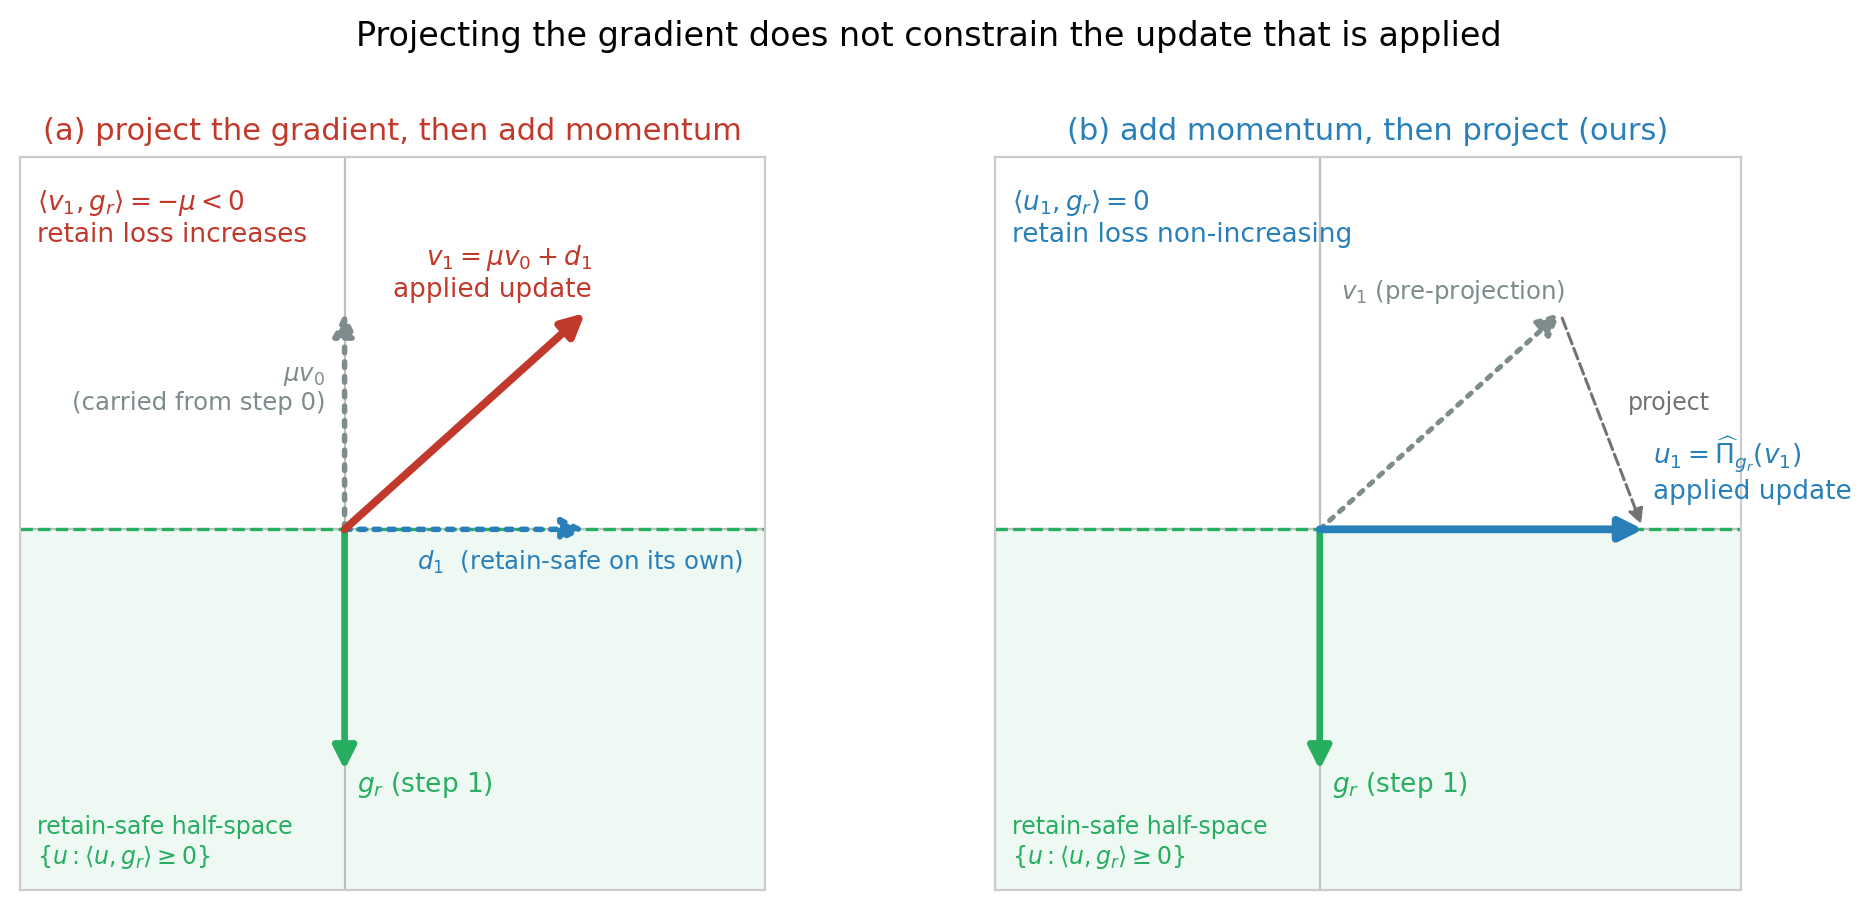
\includegraphics[width=0.86\textwidth]{fig_projection_order.png}
\caption{\textbf{Why the projection is applied to the update, not the
gradient} (Proposition~\ref{prop:counter}). Both panels show step~1, whose
constraint is $\gr$; the retain-safe half-space is shaded. \textbf{(a)}~Each
ingredient is individually retain-safe---$d_1$ lies on the boundary, and
$\mu v_0$ was certified against step~0's constraint---yet their sum, the vector
actually applied, lies in the harming half-space with
$\langle v_1,\gr\rangle = -\mu$. The violation grows with $\mu$.
\textbf{(b)}~Projecting the accumulated update instead returns it to the
boundary, so the certificate is issued against the constraint in force where
the step is taken.}
\label{fig:projorder}
\end{figure}

\subsection{Forget Objective, Stopping, and Normalisation}\label{sec:forget_obj}

The \klr{} objective drives forget-set predictions toward the retain-confusion
distribution rather than the uniform one,
\begin{equation}\label{eq:kl_retain}
\mathcal{L}_{\text{KL-R}} = \KL\!\left(\log\sigma(f_\theta(x_f)) \,\|\, p_r\right).
\end{equation}
Under the projected-momentum optimiser it forgets further than gradient ascent
\rev{and slightly further than a uniform target at equal test accuracy (FA
$2.1\%$ against $8.2\%$ and $3.9\%$, at TA $86.1$, $86.4$ and $86.4\%$; CIFAR-10
class~0, one seed)} and is within noise of a uniform target on MIA, so we claim a
better forget \emph{direction}, not a closer imitation of a retrained model
(Appendix~\ref{app:method}).

\paragraph{Dual stopping.}\label{sec:stopping}
Unlearning halts if the retain \rev{cross-entropy, measured on the full retain
set after each epoch,} exceeds $\alpha$ times its initial value, and completes
when FA reaches \rev{the target $\tau_F$}---by default the chance level
$100/K\%$---checked \rev{every $m=50$ steps} within epochs, because FA can fall
by tens of points inside one.

\paragraph{BatchNorm.}\label{sec:bn}
Class-homogeneous forget batches would corrupt BatchNorm running statistics, so
\ours{} freezes them. \added{The weights then learn to forget relative to those
frozen statistics; \S\ref{sec:bn_results} shows that this forgetting does not
survive recomputing them, and BN-robust \ours{} recomputes them from retained
data before every step instead (\S\ref{sec:bn_robust}).} A distillation anchor to
the frozen base model \rev{enters the retain objective; removing it changes
retain accuracy by only $0.04$pp on CIFAR-10 (\S\ref{sec:guarantee_measured}),
so we keep it as a safeguard rather than claim it as load-bearing}.

% ============================================================
\section{Theoretical Guarantees}\label{sec:theory}

\begin{theorem}[Exact per-step retain safety under momentum]\label{thm:retain_safety}
Let \rev{$\Lrt$, the retain objective $\lossr$ (cross-entropy plus
$\beta\losskd$) evaluated on the sampled retain mini-batch,} be $L$-smooth, and
let $\gr = \nabla_\theta\Lrt(\theta_t)$. Let \ours{} run the update of
Algorithm~\ref{alg:excise}: $\|d_t\| \le c$ by clipping,
$v_t = \mu v_{t-1} + d_t$ with $v_{-1}=0$ and $\mu \in [0,1)$,
$u_t = \Pi_{\gr}(v_t)\,\|v_t\|/\|\Pi_{\gr}(v_t)\|$ when
$\langle v_t,\gr\rangle<0$ \rev{(and $u_t=0$ if $\Pi_{\gr}(v_t)=0$)} and
$u_t = v_t$ otherwise, and $\theta_{t+1} = \theta_t - \eta u_t$. Then, exactly
and \rev{with no assumption on $\gf$ or on its alignment with $\gr$},
\begin{equation}\label{eq:thm1}
\langle u_t,\gr\rangle \ge 0,
\qquad \|u_t\| \;\rev{\le}\; \|v_t\| \;\le\; \frac{c}{1-\mu},
\qquad \Lrt(\theta_{t+1}) \;\le\; \Lrt(\theta_t) + \tfrac{1}{2}L\eta^2\Big(\frac{c}{1-\mu}\Big)^{\!2}.
\end{equation}
\end{theorem}

\begin{proof}[Proof sketch]
The first claim is immediate: if $\langle v_t,\gr\rangle \ge 0$ then $u_t=v_t$;
otherwise $\langle \Pi_{\gr}(v_t),\gr\rangle = 0$ identically, and rescaling by
a positive scalar preserves this. For the second, $\Pi_{\gr}$ is the orthogonal
projection onto $\{u : \langle u,\gr\rangle = 0\}$, so the rescaling restores
$\|u_t\|=\|v_t\|$ \rev{unless the projection vanishes}; unrolling the buffer gives
$v_t = \sum_{k=0}^{t}\mu^{t-k}d_k$, hence
$\|v_t\| \le c\sum_{j=0}^{t}\mu^{j} < c/(1-\mu)$. The third follows from
$L$-smoothness,
$\Lrt(\theta_{t+1}) \le \Lrt(\theta_t) - \eta\langle u_t,\gr\rangle
+ \tfrac{1}{2}L\eta^2\|u_t\|^2$, where the first-order term is non-positive by
claim one and $\|u_t\|$ is bounded by claim two. The full proof, together with the three supporting lemmas, is given in Appendix~\ref{app:thm1} (Theorem~\ref{thm:app_main}).
\end{proof}

The first-order change in the sampled retain loss is non-positive at every step,
and, unlike guarantees stated for momentum-free surrogates, the analysed $u_t$ is
the vector the code applies. The bound concerns the sampled mini-batch objective,
not the population retain loss (\S\ref{sec:limitations}).
\rev{Section~\ref{sec:guarantee_measured} tests the theorem on a logged run.}

\begin{theorem}[Per-step separation]\label{thm:separation}
For any model $\theta_0$ with retain gradient $\gr$:
\textbf{(i)}~GA's update $+\eta\gf$ strictly increases retain loss to first
order whenever $\langle\gf,\gr\rangle>0$;
\textbf{(ii)}~SCRUB's $-\gf+\lambda\gr$ can have $\langle\cdot,\gr\rangle<0$ for
any fixed $\lambda$;
\textbf{(iii)}~SalUn's masked random-label gradient has unconstrained sign with
respect to $\gr$;
\textbf{(iv)}~a soft conflict regulariser that adds $\rho\,\phi(\langle
g,\gr\rangle)$ with $\phi$ decreasing---the approach of the closest prior work
\citep{patel2025learning}---shifts the optimum toward positive alignment but
leaves the feasible set unrestricted: for any finite $\rho$, a sufficiently
large forget-loss reduction still makes a step with $\langle g,\gr\rangle<0$
preferable.
\rev{Among these update rules, only \ours{}'s} guarantees
$\langle u_t,\gr\rangle \ge 0$ \rev{at every step}, because only a projection
makes such steps unreachable rather than merely costly.
\end{theorem}

% ============================================================
\section{Experiments}\label{sec:experiments}

\subsection{Setup}\label{sec:setup}

We forget one class at a time on six benchmarks that vary class count, examples
per class and domain: CIFAR-10 and CIFAR-100 \citep{krizhevsky2009cifar}, MNIST
\citep{lecun1998mnist}, SVHN \citep{netzer2011svhn}, STL-10
\citep{coates2011stl10} and PathMNIST \citep{yang2023medmnist}. We forget every
class of MNIST and PathMNIST, \rev{classes $10, 20, \dots, 90$ of CIFAR-100}, and
class~0 of CIFAR-10, SVHN and STL-10 over three seeds: 31 tasks and 75 runs. All
models are ResNet-18 \citep{he2016resnet}. \rev{SalUn, SCRUB, Bad Teacher and
NegGrad+ are re-run on our stack, and a model retrained without the forget class
serves as the reference. MIA is the mean AUROC of a loss and a confidence
attack.} Hyperparameters are fixed per dataset and released as configuration
files (Appendix~\ref{app:hyper}); Appendix~\ref{app:experiments} gives the full
protocol. \rev{Table~\ref{tab:claims} lists every claim of \S\ref{sec:intro}
with the experiment that tests it; the subsections follow its order.}

\begin{table}[t]
\centering\color{revisedB}
\caption{\rev{\textbf{Each claim and the experiment that tests it.}}}
\label{tab:claims}
\small
\renewcommand{\arraystretch}{1.08}
\begin{tabular}{@{}>{\raggedright\arraybackslash}p{0.28\textwidth}>{\raggedright\arraybackslash}p{0.26\textwidth}>{\raggedright\arraybackslash}p{0.40\textwidth}@{}}
\toprule
\textbf{Claim} & \textbf{Test} & \textbf{Outcome} \\
\midrule
Forgets to chance, retain set intact & 31 tasks, six datasets (Table~\ref{tab:cross}) & Chance on all six, two at 60 epochs; RA $\ge 97.2\%$ on the 10-class datasets \\
Only \ours{} does both on CIFAR-10 & Four baselines, projection only (Table~\ref{tab:cifar10}) & FA $1.87\%$ at RA $100\%$; SalUn loses $2.9$pp RA, the rest stop at FA $\ge 18.7\%$ \\
Theorem~\ref{thm:retain_safety} holds for the optimiser that runs & Step-level audit (Figure~\ref{fig:guarantee}) & $120/120$ steps conflict before projection; $|\cos| \le 7.4\times10^{-7}$ after; $\|u_t\| \le 9.16 < 10$ \\
Soft corrections leave harm reachable (Thm.~\ref{thm:separation}) & Projection strength $s$, equal compute (\S\ref{sec:guarantee_measured}) & RA rises from $52.5$ to $99.98\%$ as $s \to 1$; every $s<1$ leaves conflict in the applied step \\
The projection protects the retain set & Ablation, equal compute (\S\ref{sec:guarantee_measured}) & Without it RA is $52.6\%$; alone it keeps RA $99.9\%$ but stops at FA $18.7\%$ \\
The guarantee must cover momentum & $\mu = 0$ ablation (Table~\ref{tab:momentum}) & With $\mu=0$, FA stays far above chance on five of six datasets \\
Frozen statistics make forgetting reversible & Recalibration attack (Table~\ref{tab:bnrecal}) & Frozen \ours{}: FA $1.4 \to 99.7\%$; base model and our baselines: $\Delta F \le 0$ \\
BN-robust \ours{} survives it & Ten classes, MNIST, attacker's data (Figures~\ref{fig:teaser}c, \ref{fig:bnrobust_attack}) & $|\Delta F| \le 0.06$pp on every CIFAR-10 class, $+0.09$pp on MNIST; attacker's data: $-1.2$ to $-1.0$pp \\
$0.5$ is the wrong MIA target & Retrained references (Table~\ref{tab:mia_main}) & References score $0.69$ (CIFAR-10) and $0.31$--$0.70$ (PathMNIST); rankings reverse \\
$p_r$ is a better direction than uniform & Forget objectives, equal TA (\S\ref{sec:forget_obj}) & FA $2.1\%$ against $3.9\%$ (uniform) and $8.2\%$ (GA); one seed \\
\bottomrule
\end{tabular}
\end{table}

\subsection{Main Results}\label{sec:main_results}

\begin{table}[t]
\centering
\caption{\textbf{Cross-dataset results.} Mean $\pm$ \rev{sample} std over
classes $\times$ seeds (3 seeds \rev{per task; one seed per class for
CIFAR-100}). \#T = number of forgetting tasks. Chance $=100/K\%$ is the level a
fully unlearned model must reach. \rev{The upper block uses each dataset's epoch
cap (12--20 epochs, Appendix~\ref{app:hyper}), which penalises datasets with few
images per class, since the binding resource is optimiser steps rather than
epochs. The lower block re-runs the two datasets that fall short at 60 epochs
($4\times$ and $3\times$ their caps), with a per-step check and a $1\%$ forget
target,} on the same seeds and classes;
$^*$marks the STL-10 row it supersedes (\S\ref{sec:crossdataset_stl}).}
\label{tab:cross}
\begin{tabular}{@{}lccccccc@{}}
\toprule
\textbf{Dataset} & \textbf{\#T} & \textbf{Chance} & \textbf{TA} & \textbf{FA}$\downarrow$ & \textbf{RA} & \textbf{MIA} \\
\midrule
CIFAR-10    & 1 & 10.0\% & $86.13 \pm 0.02$ & $\mathbf{1.87} \pm 0.25$ & $100.00 \pm 0.00$ & $0.529 \pm 0.001$ \\
MNIST       & 10 & 10.0\% & $90.00 \pm 0.64$ & $\mathbf{6.17} \pm 2.81$ & $99.49 \pm 0.04$ & $0.497 \pm 0.009$ \\
SVHN        & 1 & 10.0\% & $89.69 \pm 0.02$ & $\mathbf{5.75} \pm 0.17$ & $97.26 \pm 0.01$ & $0.525 \pm 0.001$ \\
STL-10$^*$  & 1 & 10.0\% & $92.84 \pm 0.02$ & $75.67 \pm 1.70$ & $99.38 \pm 0.10$ & $0.466 \pm 0.005$ \\
PathMNIST   & 9 & 11.1\% & $80.96 \pm 5.39$ & $\mathbf{5.82} \pm 3.42$ & $98.88 \pm 0.31$ & $0.483 \pm 0.084$ \\
CIFAR-100   & 9 & \phantom{0}1.0\% & $76.17 \pm 0.86$ & $4.07 \pm 5.51$ & $92.19 \pm 0.84$ & $0.500 \pm 0.037$ \\
\midrule
\multicolumn{7}{@{}l}{\emph{Extended budget} (\rev{60 epochs, per-step check, $1\%$ forget target}; same seeds and classes)} \\
STL-10      & 1 & 10.0\% & $85.15 \pm \rev{0.06}$ & $\mathbf{1.73} \pm \rev{0.95}$ & $98.87 \pm \rev{0.05}$ & $\rev{0.488} \pm \rev{0.008}$ \\
CIFAR-100   & 9 & \phantom{0}1.0\% & $75.50 \pm \rev{0.68}$ & $\mathbf{1.27} \pm \rev{0.39}$ & $91.32 \pm \rev{0.94}$ & $\rev{0.490} \pm \rev{0.043}$ \\
\bottomrule
\end{tabular}
\end{table}

\begin{table}[t]
\centering
\caption{\textbf{CIFAR-10 class-0 forgetting.} \ours{} is a 3-seed mean $\pm$
std. Methods with FA~$>80\%$ attain MIA~$\approx 0.5$ trivially, by barely
changing the model. $\dagger$Our reproduction; $\ddagger$our reproduction with
unified MIA. $^\S$A-GEM projection applied to plain gradient ascent, with
\ours{}'s KD anchor and retain-confusion target removed: the direct
projected-gradient baseline, isolating what the projection alone achieves.
\rev{$^\P$The retrained reference of \S\ref{sec:mia_main}; its TA and RA were
not logged, and its MIA, from the same two attacks, is $0.565$, not $0.5$.}}
\label{tab:cifar10}
\begin{tabular}{@{}lcccc@{}}
\toprule
\textbf{Method} & \textbf{TA} & \textbf{FA}$\downarrow$ & \textbf{RA} & \textbf{MIA} \\
\midrule
\rev{Retrain (reference)$^\P$} & \rev{---} & 0.0 & \rev{---} & \rev{0.565} \\
\midrule
SalUn$^\dagger$        & 84.0 & 0.0  & 97.1 & 0.497 \\
Bad Teacher$^\ddagger$ & 82.0 & 29.7 & 90.2 & 0.499 \\
SCRUB$^\ddagger$       & 93.3 & 88.8 & 97.7 & 0.515 \\
NegGrad+$^\ddagger$    & 94.2 & 84.8 & 99.3 & 0.525 \\
\midrule
Projection-only$^\S$   & 86.23 & 18.66 & 99.90 & 0.511 \\
\midrule
\textbf{\ours{}} & $\mathbf{86.13}\pm.02$ & $\mathbf{1.87}\pm.25$ & $\mathbf{100.00}\pm.00$ & $\mathbf{0.529}\pm.001$ \\
\bottomrule
\end{tabular}
\end{table}

\rev{At its epoch cap} \ours{} drives FA to or below the chance level on four
of six datasets with RA $\ge 97.2\%$ (CIFAR-100: $92.2\%$), and \rev{the mean
over seeds is below chance for every one of the ten MNIST and nine PathMNIST
classes (one of the 30 MNIST runs ends at $10.2\%$, within sampling error)}
(Table~\ref{tab:cross}, Appendix~\ref{app:perclass}). The two shortfalls are
budget-limited: STL-10 gets ${\sim}60$ optimiser steps at \rev{its 15-epoch cap}
against ${\sim}600$ for CIFAR-10 \rev{at the same cap}, and at 60 epochs
\rev{(per-step check, $1\%$ target)} STL-10 reaches $1.73\%$ \rev{($9.2\%$ in a
single run at its default $10\%$ target)} and CIFAR-100 $1.27\%$\rev{---against a $1\%$ chance level,
within one standard error of a 500-image forget set}---so all six datasets reach
chance. On CIFAR-10 (Table~\ref{tab:cifar10}, \rev{Figure~\ref{fig:teaser}b}),
\ours{} is the only method \rev{in the table} that both forgets to chance
and leaves retain accuracy untouched: SalUn forgets fully but costs $2.9$pp of
retain accuracy, Bad Teacher stops at $29.7\%$ while damaging the model, and
SCRUB and NegGrad+ keep the model intact by barely forgetting. The projection
alone does not unlearn: applied to plain gradient ascent it preserves the retain
set but stalls at $18.66\%$, so the projection supplies retain safety and the
\klr{} objective supplies the forgetting.

\subsection{The Guarantees, Measured}\label{sec:guarantee_measured}

\begin{figure}[t]
\centering
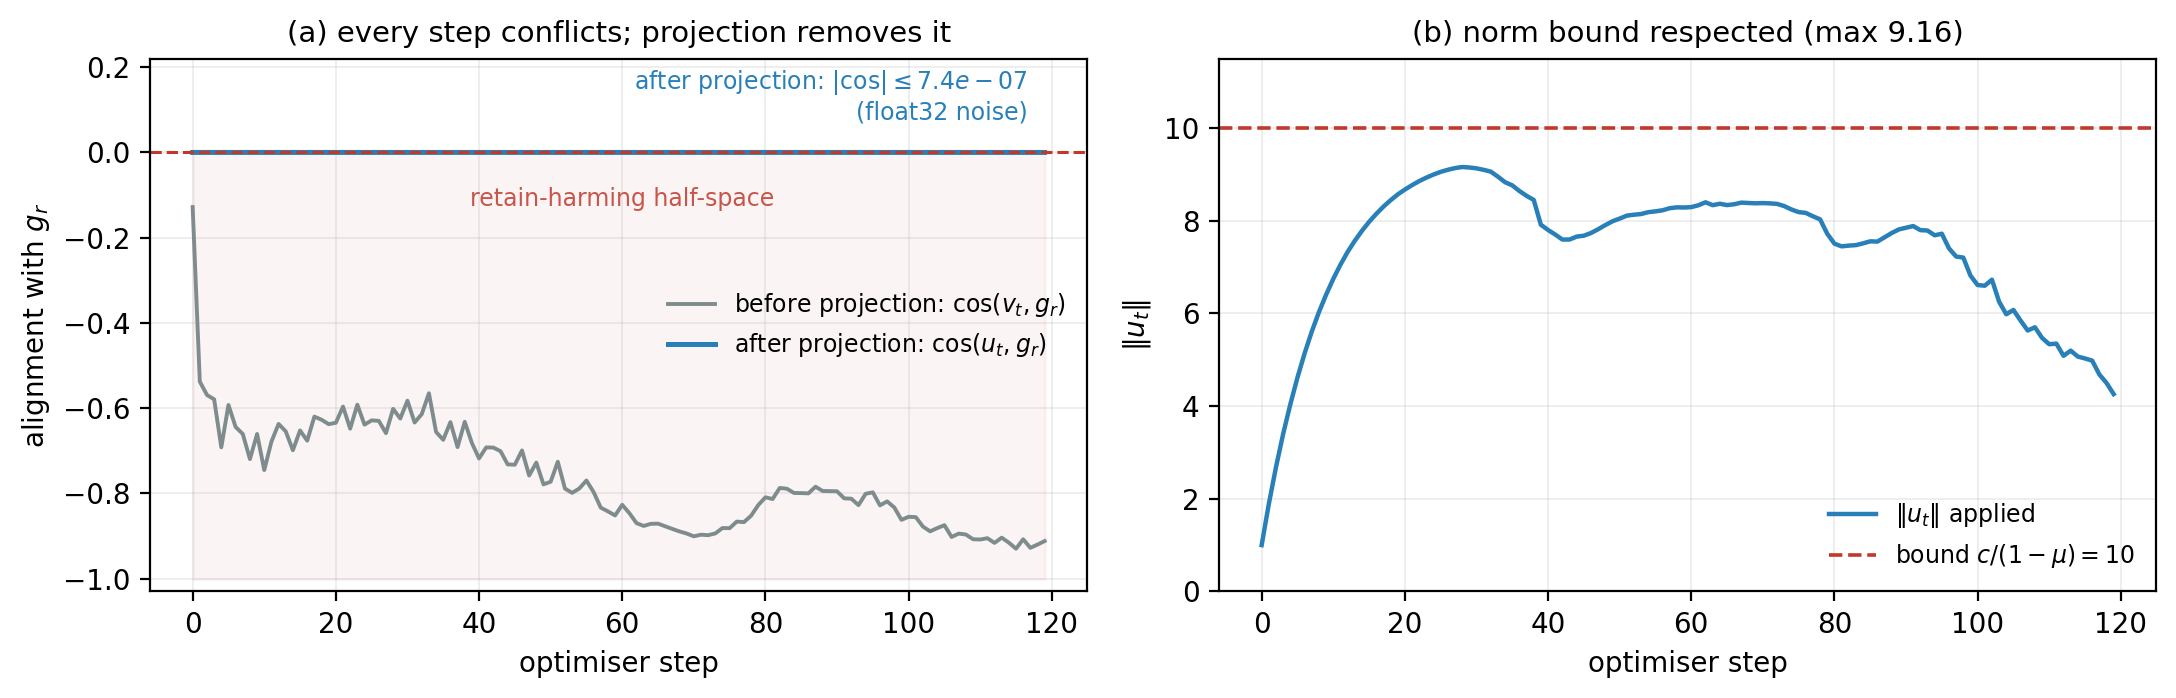
\includegraphics[width=0.86\textwidth]{fig_guarantee.png}
\caption{\textbf{Theorem~\ref{thm:retain_safety} audited on a real run}
(CIFAR-10 class~0, 120 steps). \textbf{(a)}~Alignment with the retain gradient,
normalised to $\cos(\cdot,\gr)$. Before projection every step lies in the
retain-harming half-space (mean $-0.77$); after projection the alignment is
indistinguishable from zero ($|\cos| \le 7.4\times10^{-7}$, the float32
accumulation scale). \textbf{(b)}~The applied update never exceeds the bound
$c/(1-\mu)=10$ of Eq.~\ref{eq:thm1}, peaking at $9.16$---tight, but respected.}
\label{fig:guarantee}
\end{figure}

\rev{\paragraph{Theorem~\ref{thm:retain_safety} on a real run.}
We log every step of a CIFAR-10 run (class~0, 120 steps;
Figure~\ref{fig:guarantee}, Appendix~\ref{sec:alignment}). The accumulated update
conflicts with the retain gradient at all 120 steps (mean
$\cos(v_t,\gr) = -0.77$), so the projection is the optimiser's defining step
rather than a safeguard. After projection the alignment is zero to float32
precision ($|\cos(u_t,\gr)| \le 7.4\times10^{-7}$), and $\|u_t\|$ peaks at
$9.16$ against the bound $c/(1-\mu)=10$.

\paragraph{Theorem~\ref{thm:separation}(iv): soft against hard.}
To test the separation without reimplementing another method, we vary our own
projection between a soft correction and the hard constraint: at conflicting
steps $u = v - s\,\frac{\langle v,\gr\rangle}{\|\gr\|^2}\gr$, so
$\langle u,\gr\rangle = (1-s)\langle v,\gr\rangle < 0$ for every $s<1$. At equal
compute with stopping disabled every setting forgets completely (FA $0.0\%$), so
the settings differ only in collateral damage: RA is $52.5$, $81.4$, $92.8$,
$98.2$ and $99.98\%$ for $s = 0, 0.25, 0.5, 0.75, 1$ (Appendix~\ref{sec:strength}).
The curve is gradual---$s=0.75$ already keeps $98.2\%$---so the case for $s=1$
is that it is the only setting with a guarantee, not that the last $1.8$pp is
large.

\paragraph{The projection is what protects the retain set.}
At equal compute with stopping disabled, removing the projection collapses the
model (TA $44.4\%$ and RA $52.6\%$, against $85.7\%$ and $99.98\%$ with it),
removing the distillation anchor changes RA by $0.04$pp, and the projection on
its own keeps RA at $99.9\%$ but stalls at FA $18.7\%$
(Tables~\ref{tab:cifar10} and~\ref{tab:ablation}). With stopping enabled every
variant halts after one epoch and the projection looks costless, which is why we
report both modes.}

\subsection{Momentum Is Not Incidental}\label{sec:momentum_ablation}

\begin{table}[t]
\centering
\caption{\textbf{Momentum ablation.} Removing momentum to simplify the analysis
\rev{leaves forget accuracy far above chance on five of six datasets; on STL-10
projected momentum also falls short at this budget (Table~\ref{tab:cross})}.
High RA with high FA indicates the model barely changed. Same configs, seeds,
and stopping rules throughout.}
\label{tab:momentum}
\begin{tabular}{@{}lccccc@{}}
\toprule
& & \multicolumn{2}{c}{$\mu=0$ (analysis-friendly)} & \multicolumn{2}{c}{Projected momentum (ours)} \\
\cmidrule(lr){3-4}\cmidrule(lr){5-6}
\textbf{Dataset} & \textbf{Chance} & \textbf{FA}$\downarrow$ & \textbf{RA} & \textbf{FA}$\downarrow$ & \textbf{RA} \\
\midrule
CIFAR-10  & 10.0\% & \phantom{0}5.8 & 100.0 & \phantom{0}1.9 & 100.0 \\
MNIST     & 10.0\% & 95.9 & \phantom{0}99.5 & \phantom{0}6.2 & 99.5 \\
SVHN      & 10.0\% & 61.9 & \phantom{0}97.4 & \phantom{0}5.8 & 97.3 \\
STL-10    & 10.0\% & 99.7 & \phantom{0}99.4 & 75.7 & 99.4 \\
PathMNIST & 11.1\% & 16.4 & \phantom{0}99.0 & \phantom{0}5.8 & 98.9 \\
CIFAR-100 & \phantom{0}1.0\% & 73.7 & \phantom{0}94.1 & \phantom{0}4.1 & 92.2 \\
\bottomrule
\end{tabular}
\end{table}

Removing momentum is the most direct route to an exact guarantee, since the
applied update then equals the projected gradient. Table~\ref{tab:momentum} shows
the cost: with $\mu = 0$ and everything else fixed, \rev{forget accuracy stays
far above chance on five of six datasets} (FA $95.9\%$ on MNIST, $99.7\%$ on
STL-10, $73.7\%$ on CIFAR-100), and RA stays high only because the model barely
moves. \rev{STL-10 does not forget at this budget with momentum either
($75.7\%$), so the comparison rests on the other four: without momentum all four
stay far above chance; with it, three reach chance and CIFAR-100 ends at
$4.1\%$.} A guarantee stated for the momentum-free update would be exact and
would describe a method that does not unlearn. The dependence is not ours alone:
every update rule we tested loses forgetting without momentum, but the KL
objectives lose $70$--$79$pp against $12$--$15$pp for gradient ascent \rev{(with
or without projection; means over MNIST and SVHN), consistent with a bounded
objective needing} momentum's $1/(1-\mu)$ amplification
(Appendix~\ref{app:momentum}).

\subsection{BatchNorm: the Attack, and a Fix That Keeps BatchNorm}\label{sec:bn_results}

\begin{table}[t]
\centering
\caption{\textbf{BatchNorm recalibration} (CIFAR-10, class~0), using
\texttt{update\_bn} on the retain set: BatchNorm buffers are reset and
recomputed, no weight is touched. \rev{Our reproductions of the baselines}
and the un-unlearned base model are unaffected ($\Delta F \le 0$); \ours{} with a
BatchNorm backbone loses essentially all of its forgetting. The two backbones without running statistics
are outside the operator's reach by construction. NegGrad+ is omitted: no
checkpoint for it was available.}
\label{tab:bnrecal}
\begin{tabular}{@{}lccccc@{}}
\toprule
Configuration & pre-$F$ & post-$F$ & $\boldsymbol{\Delta F}$ & pre-TA & post-TA \\
\midrule
Base model (no unlearning)  & $100.0$ & $99.8$ & $-0.2$ & $95.5$ & $92.9$ \\
SalUn                       & $0.0$   & $0.0$  & $+0.0$ & $84.7$ & $84.4$ \\
Bad Teacher                 & $28.7$  & $28.4$ & $-0.3$ & $81.5$ & $84.0$ \\
SCRUB                       & $89.3$  & $85.7$ & $-3.6$ & $93.5$ & $93.2$ \\
\midrule
\ours{} (BatchNorm, frozen) & $1.4$   & $99.7$ & $\mathbf{+98.4}$ & $86.1$ & $92.9$ \\
\ours{} (GroupNorm)         & $4.9$   & $4.9$  & $\mathbf{0.0}$   & $84.2$ & $84.2$ \\
\ours{} (ViT-B/16, LayerNorm) & $9.6$ & $9.6$  & $\mathbf{0.0}$   & $87.0$ & $87.0$ \\
\bottomrule
\end{tabular}
\end{table}

\begin{table}[t]
\centering\color{revised}
\caption{\added{\textbf{BN-robust \ours{} under BatchNorm recalibration} (CIFAR-10,
class~0, seeds $\{42,123,456\}$; \texttt{update\_bn} on the retain set, as in
Table~\ref{tab:bnrecal}). Every row shares the $93.97\%$ base except GroupNorm,
which needs its own. The un-unlearned base is the control: recalibrating it
changes nothing. \emph{Naive} stopping reads FA under the in-loop statistics,
\emph{calibrated} stopping under the statistics that ship. Time is wall-clock per
run on one GPU.}}
\label{tab:bnrobust}
\small
\setlength{\tabcolsep}{4pt}
\begin{tabular}{@{}lcccccccc@{}}
\toprule
Configuration & base TA & pre-$F$ & post-$F$ & $\boldsymbol{\Delta F}$ & TA & RA & epochs & min \\
\midrule
Base model (no unlearning)     & $93.97$ & $99.80$ & $99.82$ & $+0.0$ & $93.97$ & ---     & ---          & ---    \\
\ours{} (BatchNorm, frozen)    & $93.97$ & $8.51 \pm 0.30$  & $99.12 \pm 0.09$ & $\mathbf{+90.6}$ & $85.20$ & $97.34$ & $2$          & $1.9$  \\
\ours{} (GroupNorm)            & $91.89$ & $5.91 \pm 0.09$  & n/a              & n/a              & $83.13$ & $98.92$ & $3$          & $2.5$  \\
BN-robust, naive stopping      & $93.97$ & $11.43 \pm 1.90$ & $11.44 \pm 1.87$ & $\mathbf{0.0}$   & $84.42$ & $95.46$ & $11$--$13$   & $9.8$  \\
BN-robust, calibrated stopping & $93.97$ & $9.19 \pm 0.08$  & $9.18 \pm 0.07$  & $\mathbf{0.0}$   & $84.30$ & $95.59$ & $13$         & $13.3$ \\
\bottomrule
\end{tabular}
\end{table}

\paragraph{The attack.}
\texttt{update\_bn} resets every BatchNorm buffer and recomputes the statistics
on the retain set without touching a weight; we verify that every learnable
parameter is bit-identical afterwards. Table~\ref{tab:bnrecal} shows that
recalibration leaves the un-unlearned base model and every baseline we
reproduced unaffected, but undoes \ours{} with frozen statistics completely:
forget accuracy returns from $1.4\%$ to $99.7\%$ and test accuracy to $92.9\%$,
\rev{the value recalibration gives the base model itself}. Because the
statistics are frozen, the weights learn to forget against statistics an
attacker can replace. \rev{Our baseline reproductions survive because each ends
every epoch with a pass over retained data in train mode, which recomputes the
statistics. Under their reference implementations, \citet{kalani2026batchnorm}
recover six of nine prior methods, and find SalUn's recovery disappears once at
least a quarter of each unlearning batch is retained data.} GroupNorm and a ViT's
LayerNorm keep no running statistics and are outside the attack's reach by
construction (Tables~\ref{tab:gn} and~\ref{tab:vit}), but that is a change of
architecture, not robustness.

\paragraph{BN-robust \ours{}.}\label{sec:bn_robust}
\added{We keep BatchNorm and stop the statistics going stale. Before every step
they are recomputed on 512 retain images with the attacker's own operator, after
the last step on the whole retain set, and the stopping rule reads forget
accuracy under the statistics that will ship, falling back to the best epoch if
the target is not met (\rev{Figure~\ref{fig:bnrobust_mech}, Appendix~\ref{app:bn_robust}}). The update rule is
unchanged, \rev{so Theorem~\ref{thm:retain_safety} holds at every step for the
retain objective under the statistics in force during that step; the
recalibration between steps is not a gradient step, and the theorem does not
bound its effect}. Table~\ref{tab:bnrobust} gives the
result on a separate base model (the checkpoints behind Table~\ref{tab:bnrecal}
were no longer available): with frozen statistics the attack returns forget
accuracy to $99.1\%$, while BN-robust \ours{} forgets to $9.2\%$ and stays at
$9.2\%$. It holds on all ten CIFAR-10 classes ($6.7$--$10.2\%$ after the attack,
all within three standard errors of chance), on MNIST ($3.9\%$, where frozen
statistics recover to $99.97\%$), and when the attacker recalibrates on the full
training set or the test set instead \rev{(tested on the naive-stopping
checkpoints, whose FA moves by $-1.2$ to $-1.0$pp)} (Figure~\ref{fig:bnrobust_attack},
Appendix~\ref{app:bn_robust}). It costs
about seven times the compute and $1.8$pp of retain accuracy, mostly because
forgetting that must happen in the weights takes ${\sim}13$ epochs
instead of~$2$.}

\begin{figure}[t]
\centering\color{revised}
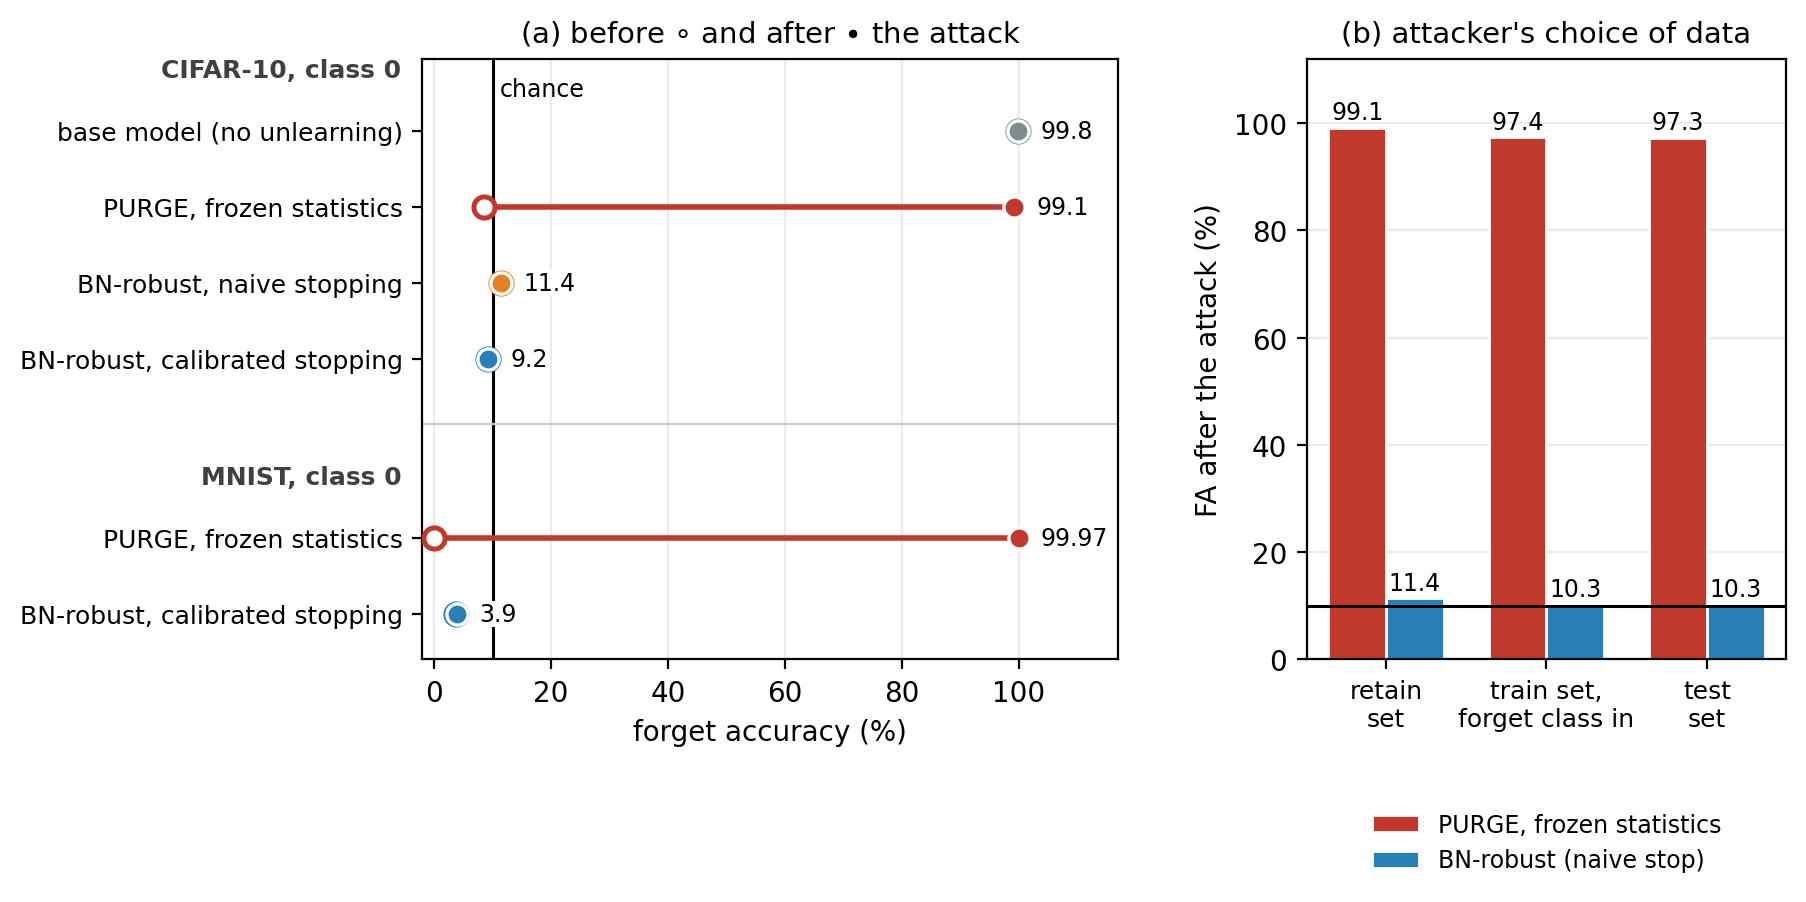
\includegraphics[width=\textwidth]{fig_bnrobust_attack.png}
\caption{\added{\textbf{BN-robust survives the recalibration attack.} (a)~Forget
accuracy before (open) and after (filled) \texttt{update\_bn} on the retain set,
class~0, means over three seeds; on MNIST the frozen configuration's forgetting
is undone completely. (b)~Forget accuracy after the attack when the attacker
recalibrates on the retain set, the full training set (forget class included),
or the test set (CIFAR-10 class~0, three seeds; BN-robust with naive stopping).}}
\label{fig:bnrobust_attack}
\end{figure}

\subsection{Membership Inference Needs a Retrained Reference}\label{sec:mia_main}

\rev{MIA is usually read against $0.5$: an attacker should not be able to tell
forget-class training samples from forget-class test samples. We test that
target against models retrained without the forget class, which trained on
neither group (Table~\ref{tab:mia_main}; Appendix~\ref{sec:mia} adds three
attacks). On CIFAR-10 the reference scores $0.694$ on the loss attack, with a
true-positive rate of $12.5\%$ at $1\%$ false positives, while the base model,
which memorised every member, scores $0.483$: the attack reads a difference in
difficulty between the train and test splits, not membership. Across four
PathMNIST classes the reference ranges from $0.306$ to $0.704$, so no single
constant is the right target. Read against $0.5$, \ours{} looks the worst of the
four methods on CIFAR-10 and SalUn the best; read against the reference, the
order reverses. SalUn's $0.500$ is also degenerate: its true-positive rate is
zero at every threshold, the signature of a constant score. On three of the four
PathMNIST classes \ours{} sits far from its own reference (mean gap
$0.22$--$0.36$ over four attacks), so we claim the protocol finding, not that
\ours{} matches retrained models in general.}

\begin{table}[t]
\centering\color{revisedB}
\caption{\rev{\textbf{Loss-attack MIA against a retrained reference}
(CIFAR-10, class~0). Members are the $5000$ forget-class training images,
non-members the $1000$ forget-class test images; TPR is at $1\%$ FPR.
Appendix~\ref{sec:mia} gives three further attacks and four PathMNIST classes.}}
\label{tab:mia_main}
\small
\begin{tabular}{@{}lccccc@{}}
\toprule
Model & FA & AUROC & TPR & $|\mathrm{AUROC}-0.5|$ & $|\mathrm{AUROC}-\mathrm{ref}|$ \\
\midrule
Retrained (reference) & $0.0$   & $0.694$ & $12.5\%$ & $0.194$ & ---   \\
Base (no unlearning)  & $100.0$ & $0.483$ & $0.0\%$  & $0.017$ & $0.211$ \\
\midrule
SalUn                 & $0.0$   & $0.500$ & $0.0\%$  & $\mathbf{0.000}$ & $0.194$ \\
Bad Teacher           & $24.8$  & $0.485$ & $0.2\%$  & $0.015$ & $0.209$ \\
SCRUB                 & $89.5$  & $0.477$ & $0.4\%$  & $0.023$ & $0.217$ \\
\ours{}               & $2.0$   & $0.693$ & $1.4\%$  & $0.193$ & $\mathbf{0.001}$ \\
\bottomrule
\end{tabular}
\end{table}

\subsection{Further Analyses}\label{sec:further}

The appendices report the remaining experiments in full. \emph{Transformer:} on
ViT-B/16 forgetting transfers \rev{on CIFAR-10}, with FA $9.71\%$ and RA
$97.55\%$, \rev{but not on CIFAR-100 within its 20-epoch cap, where FA ends
between $4.0\%$ and $82.0\%$ across nine classes against a $1\%$ chance level}
(Appendix~\ref{sec:vit}). \emph{Tolerances:} the retain budget is non-binding,
and the forget target is a usable knob over a $29$pp range once it is checked at
every step (Appendix~\ref{sec:sweeps}). \emph{Distance to a retrained model:}
\ours{} is closest in feature space (Fr\'echet distance $13$ against
$153$--$495$ for the baselines) and SalUn in output space
(Appendix~\ref{sec:distance}). \emph{Stopping point:} divergence to a retrained
model is U-shaped along the trajectory with its minimum above chance, and MIA
passes through $0.5$ rather than converging to it
(Appendices~\ref{sec:overforget} and~\ref{sec:trajectory}). \rev{\emph{Sequential
unlearning:} over three classes TA falls from $86.1\%$ to $69.1\%$ and RA from
$100\%$ to $80.7\%$, no more than the forgotten classes themselves account for
(\S\ref{sec:limitations}).}

% ============================================================
\section{Limitations}\label{sec:limitations}

The compute a dataset needs cannot be predicted in advance: the binding resource
is optimiser steps, and STL-10 and CIFAR-100 needed 60 epochs rather than 15 and
20\rev{; ViT-B/16 on CIFAR-100 does not reach chance within its 20-epoch cap}.
Sample-level forgetting works only crudely, because the retain-confusion
target degenerates to uniform when every class remains in the retain set. The
guarantee bounds the sampled mini-batch retain objective, not the population
loss, and holds to float32 precision\rev{; under BN-robust \ours{} it holds per
step under that step's statistics and does not cover the recalibration between
steps}. Our separation from soft conflict-resolution methods
\citep{patel2025learning} is structural; we have not run that method on our
stack. BN-robust \ours{} costs about seven times the compute, was evaluated on
two datasets, and defends only the normalisation statistics, not weight-level
attacks such as fine-tuning recovery\rev{; its comparison with prior methods
rests on the evaluations of \citet{kalani2026batchnorm} and on our own
reproductions, and a like-for-like run of those methods under the same base and
attack remains to be done. In sequential unlearning the retained classes are not
damaged cumulatively, but earlier-forgotten classes partly return: after three
classes RA is $80.7\%$, above the $77.8\%$ that fully forgotten classes would
allow, so they average at least $13\%$ training accuracy, above chance.} \ours{}
gives no differential-privacy guarantee. Appendix~\ref{app:limitations}
discusses each point.

% ============================================================
\section{Conclusion}\label{sec:conclusion}

Unlearning is the dual of continual learning, and \rev{one of continual
learning's most direct tools, a hard constraint on the update, carries over}.
For that constraint to mean anything it must be stated for the update the
optimiser applies: projecting the post-momentum update makes
Theorem~\ref{thm:retain_safety} exact for the deployed optimiser, while the
analysis-friendly alternative \rev{leaves forget accuracy far above chance on
five of six datasets}. Across six datasets and 31 forgetting tasks \ours{}
reaches the chance level on all six (two at a longer budget) with retain
accuracy at or above $97.2\%$ on the 10-class datasets, and \rev{step-level logs
of a CIFAR-10 run} confirm the constraint at every step.
\added{On BatchNorm backbones, keeping the normalisation statistics consistent
with the weights throughout unlearning makes that forgetting survive
recalibration, on every CIFAR-10 class and on MNIST.} The duality is also a
design space: \rev{many continual-learning techniques that protect old-task
knowledge suggest unlearning counterparts} that protect retained knowledge
during erasure. More broadly, when an
optimiser detail is chosen for analytical convenience, it should be checked
against the behaviour it was meant to explain.

\FloatBarrier
% tmlr.bst when available; plainnat keeps the document compilable without it.
\IfFileExists{tmlr.bst}{\bibliographystyle{tmlr}}{\bibliographystyle{plainnat}}
\bibliography{../references}

% ============================================================
\appendix
% ============================================================
\section{Related Work and Positioning in Full}\label{app:related}\label{sec:related_intro}

Approximate unlearning methods occupy different points on the privacy--utility
frontier, and the retain side is where they differ most. \textbf{Gradient
ascent} \citep{thudi2022unrolling} maximises forget-set loss with no mechanism
protecting retain accuracy \rev{(Theorem~\ref{thm:separation}(i))}. \textbf{SalUn} \citep{fan2024salun} confines random-label updates to a
saliency mask---effective in practice, but with no formal retain guarantee and
no control over how much is forgotten. \textbf{SCRUB}
\citep{kurmanji2023unbounded} alternates forget and retain steps balanced by a
weight $\lambda$, so the balance is tuned rather than enforced; in our
reproduction it preserves retain accuracy ($97.7\%$) by barely forgetting at all
(forget accuracy $88.8\%$, Table~\ref{tab:cifar10}). \textbf{NegGrad+}
\citep{thudi2022unrolling} adds a retain-loss term as a weighted sum, again
without a guarantee that retain loss is controlled. Closest to us,
\citet{patel2025learning} diagnose the same forget--retain gradient conflict but
resolve it with a soft regulariser that rewards positive alignment. A fuller treatment, including exact unlearning and distillation-based methods, follows the table.

The distinction we draw is structural rather than numerical, so
Table~\ref{tab:properties} compares properties of each method's \emph{definition}
---checkable against the published update rule, without relying on our
reimplementation of it. A soft penalty biases the optimiser toward retain-safe
steps but leaves harmful steps feasible: for any finite penalty weight, a
sufficiently large forget-loss reduction still makes a retain-harming step
preferable. A projection removes those steps from the feasible set altogether
(Theorem~\ref{thm:separation}(iv)). The final row is the one we would emphasise,
and the one \S\ref{sec:momentum_ablation} makes concrete: a guarantee proved for
a momentum-free surrogate says nothing about a run that uses momentum.

\rev{Figure~\ref{fig:teaser}} places the method against the alternatives on both
what it achieves and what it guarantees.

\paragraph{Exact unlearning.}
SISA \citep{bourtoule2021sisa} partitions data into shards so that removal
requires retraining only the affected shard; the per-deletion cost approaches
full retraining as shard count grows. Certified removal
\citep{guo2020certified} gives exact guarantees for convex models but does not
extend to deep networks.

\paragraph{Gradient-based approximate unlearning.}
GA \citep{thudi2022unrolling} maximises forget-set loss, with no mechanism to
prevent the same direction from degrading retain performance. Amnesiac
unlearning \citep{graves2021amnesiac} subtracts cached per-sample updates,
requiring $O(T|\Df|)$ storage. NegGrad+ optimises
$-\lossf + \lambda\lossr$ directly, which is the Lagrangian relaxation of
Eq.~\ref{eq:problem} rather than a solution to it: the retain term shifts the
optimum without bounding any single step, so the weighted sum is exactly the
soft treatment Theorem~\ref{thm:separation}(iv) separates us from.

\paragraph{Saliency and Fisher methods.}
SalUn \citep{fan2024salun} applies random-label updates inside a top-50\%
saliency mask: strong empirically (FA~$=0\%$ on CIFAR-10) but with no formal
retain guarantee and no control over the degree of forgetting. Fisher-based
methods \citep{golatkar2020eternal,golatkar2021scrubbing} and SSD
\citep{foster2024ssd} weight parameters by estimated importance, requiring
Hessian approximations that scale poorly.

\paragraph{Knowledge distillation.}
Bad Teacher \citep{chundawat2023badteacher} uses competent/incompetent teachers.
SCRUB \citep{kurmanji2023unbounded} is closest in motivation---both draw on CL
intuitions and use KD to anchor retain behaviour---but differs algorithmically:
SCRUB alternates forget and retain steps balanced by $\lambda$, so its balance is
hyperparameter-dependent, whereas \ours{}'s retain safety holds by construction
(Theorem~\ref{thm:separation}); and SCRUB ascends the forget loss, which is
unstable in either direction, whereas \klr{} converges to a specific target
distribution.

\paragraph{Continual learning connection, and the closest prior work.}
A-GEM \citep{chaudhry2019agem} projects task gradients to avoid catastrophic
forgetting. The CL--MU duality has been noted conceptually
\citep{nguyen2020variational,kurmanji2023unbounded}. Closest to \ours{}, recent
work \citep{patel2025learning} also targets the forget--retain gradient
conflict, but through an \emph{implicit, soft} regulariser encouraging a positive
inner product---with no per-step constraint and no formal guarantee. More
broadly, gradient projection and conflict resolution are now actively explored
for unlearning. \added{Closest in mechanism is Projected-Gradient Unlearning
\citep{hoang2024learn}, which takes unlearning steps orthogonal to a gradient
subspace estimated for the retained data. \ours{} differs in the constraint and in
what it binds: a half-space against the current retain gradient---the minimum
correction that excludes retain-harming steps---applied to the post-momentum
update the optimiser actually takes.} \ours{} enforces $\langle u_t,\gr\rangle \ge 0$ explicitly at every
step, on the post-momentum update, which is the difference between \emph{softly
discouraging} conflict and \emph{provably eliminating} it---and, relative to
guarantees stated for momentum-free surrogates, the difference between a bound
that describes the deployed optimiser and one that does not.
\S\ref{sec:strength} tests the mechanism this distinction rests on by varying
our own projection between a soft penalty and the hard constraint; a
like-for-like run of that method on our stack remains future work.

% ============================================================
\section{Design Details}\label{app:method}

\subsection{From the Optimisation Problem to the Algorithm}

This framing makes three things explicit that weighted multi-objective
approaches conflate. First, retain safety is a \emph{hard constraint}, not a
soft penalty. Second, \rev{the forget objective sets the direction of the
search and the forget-accuracy target its end point; only the second is a
constraint}. Third, the two tolerances \rev{$(\alpha, \tau_F)$} are quantities a
practitioner sets, not epochs to be tuned.

\paragraph{Why this needs a new algorithm.} Writing down
Eq.~\ref{eq:problem} is not by itself progress: one could hand it to a generic
constrained solver, or relax it into the weighted objective that existing
methods already optimise. Both routes lose the property we are after. A
Lagrangian relaxation replaces the retain constraint with a penalty
$\lambda\,\lossr$, which is precisely the soft treatment whose feasible set still
contains retain-harming steps (Theorem~\ref{thm:separation}(iv)); and a
projected-gradient solver applied naively would enforce feasibility on the
gradient while the optimiser applies something else
(Proposition~\ref{prop:counter}). What the problem \emph{does} buy is a
specification: it says exactly which quantity each mechanism must control.
\rev{\ours{} realises each condition with the cheapest mechanism we know that
enforces it, and enforces retain safety at every step on the vector actually
applied.} Table~\ref{tab:constraint_map} states that correspondence, and
\S\ref{sec:method} derives each row.

\begin{table}[t]
\centering
\caption{\rev{\textbf{From the problem to the algorithm.} Each condition of
Eq.~\ref{eq:problem}, and the property of the search path, with the mechanism
that enforces it. Two components serve no condition directly: the distillation
anchor, which is part of the retain objective the projection protects, and the
handling of BatchNorm statistics (\S\ref{sec:bn}).}}
\label{tab:constraint_map}
\color{revisedB}
\begin{tabular}{@{}p{0.31\textwidth}p{0.33\textwidth}p{0.28\textwidth}@{}}
\toprule
\textbf{Condition} & \textbf{Mechanism} & \textbf{Enforced} \\
\midrule
Retain objective does not increase along the path &
Projection of the post-momentum update onto $\{\langle u,\gr\rangle \ge 0\}$ (\S\ref{sec:projection}--\ref{sec:optimiser}) &
Every step, to first order on the sampled batch (Thm.~\ref{thm:retain_safety}) \\
\addlinespace
$\CE(\theta;\Dr) \le \alpha\,\CE(\theta_0;\Dr)$ &
Retain-loss stopping rule (\S\ref{sec:stopping}) &
After every epoch, on the full retain set \\
\addlinespace
$\mathrm{FA}(\theta;\Df) \le \tau_F$ &
Forget-accuracy stopping rule (\S\ref{sec:stopping}) &
Every $m$ steps \\
\addlinespace
Direction of the search &
\klr{}: descend $\KL(p_\theta(x_f)\|p_r)$ (\S\ref{sec:forget_obj}) &
Every step \\
\addlinespace
$\|\theta - \theta_0\| \le R$ &
Clipping before accumulation, and the step budget &
$\|\theta_N - \theta_0\| \le N\eta c/(1-\mu)$ \\
\bottomrule
\end{tabular}
\end{table}

\subsection{What Is Taken from A-GEM, and What Is Not}

The operator in
Eq.~\ref{eq:projection} is A-GEM's, and we claim no novelty for it: the
correction $v \mapsto v - \frac{\langle v,g\rangle}{\|g\|^2}g$ is the standard
projection onto a half-space, and \citet{chaudhry2019agem} introduced its use in
continual learning with $g$ the gradient on an episodic memory of past tasks. We
also inherit its two attractive properties: it is the \emph{minimum-norm}
correction restoring feasibility, so it is the least destructive repair of a
conflicting step, and it costs one extra backward pass and one inner product per
step.

What is new is what the operator is asked to do. In A-GEM the projection is a
safeguard on a process whose objective already points the right way---the new
task is being learned, and the memory gradient only occasionally interferes; in
our runs the conflict is not occasional but universal, firing at $100\%$ of
steps (\S\ref{sec:alignment}), because erasing a class and preserving the rest
are directly opposed rather than incidentally so. The projection is therefore
not a correction applied to an optimiser but the optimiser's defining step. That
change of role has three consequences, and they are what
\S\ref{sec:optimiser} is about:
\begin{enumerate}
\item \emph{It must bind the applied vector.} A-GEM projects a gradient; with
momentum the applied vector is not the gradient, and projecting the gradient
certifies nothing (Proposition~\ref{prop:counter}).
\item \emph{Its magnitude matters.} A-GEM tolerates $\|\Pi_{\gr}(v)\| \le \|v\|$
because progress on the new task comes mostly from unconflicted steps. When
every step conflicts, that contraction compounds and forgetting stalls, so we
restore the norm after projecting.
\item \emph{It bounds nothing on the forget side.} The projection guarantees
retain safety and only that; on its own it does not unlearn. Our projection-only
ablation reaches forget accuracy $18.66\%$ against a $10\%$ chance level
(Table~\ref{tab:cifar10}), which is why \ours{} pairs it with a forget objective
rather than presenting the projection as a method.
\end{enumerate}

\subsection{The Three Ordering Choices}

\ours{} uses SGD with momentum $\mu$, weight decay $\lambda_{\mathrm{wd}}$, and
gradient clipping $c$. Three ordering choices determine whether the guarantee is
real, and all three matter empirically.

\paragraph{(i) Project the update, not the gradient.}
The vector applied to the weights is $u_t$, not $\gf$. We therefore
momentum-accumulate first and project afterwards
(Algorithm~\ref{alg:excise}, lines 10--15), so that
$\langle u_t,\gr\rangle \ge 0$ holds for the update that is actually applied.
Projecting $\gf$ instead leaves $\langle u_t,\gr\rangle$ unconstrained.

\paragraph{(ii) Clip before accumulating.}
Clipping is applied to the per-step ingredient $d_t$ \emph{before} it enters the
momentum buffer. This preserves the standard SGD semantics in which momentum
accumulates clipped gradients, and yields the bound
$\|v_t\| \le c/(1-\mu)$ used in Theorem~\ref{thm:retain_safety}. Clipping the
final update instead would cap $\|u_t\| \le c$, destroying the
$1/(1-\mu)$ amplification that momentum provides; since raw forget gradients are
${\sim}100\times$ the clip threshold in our runs, clipping is always active, and
this ordering is the difference between forgetting and not forgetting.

\paragraph{(iii) Preserve magnitude under projection.}
Projection is norm-non-increasing: $\|\Pi_{\gr}(v)\| = \|v\|\sin\vartheta$ where
$\vartheta$ is the angle between $v$ and $\gr$. When forget and retain gradients
are nearly antiparallel, $\sin\vartheta \approx 0$ and the applied step
collapses, stalling forgetting for reasons unrelated to retain safety. We
therefore rescale the projected update to the pre-projection norm,
$u_t = \Pi_{\gr}(v_t)\,\|v_t\|/\|\Pi_{\gr}(v_t)\|$. Because
$\langle u,\gr\rangle = 0$ is invariant to positive rescaling, this leaves the
guarantee untouched while decoupling forgetting speed from conflict severity.
(If $\Pi_{\gr}(v_t)=0$, i.e.\ $v_t$ is exactly antiparallel to $\gr$, we set
$u_t=0$; the guarantee holds trivially.)

\subsection{The Forget Objective}

The \klr{} objective of Eq.~\ref{eq:kl_retain} targets $p_r$,
where $p_r$ (Eq.~\ref{eq:retain_confuse}) is the model's natural confusion
pattern. The motivation is that no trained model produces uniform outputs, so a
model driven toward $\mathcal{U}(K)$ remains separable from a retrained one even
at FA~$=0\%$; a forget target drawn from the model's own behaviour on retained
data does not have that artefact. Under the previous implementation this was
supported empirically, with the uniform target giving MIA AUROC~$=0.469$ against
$0.496$ for \klr{}. \textbf{Re-measured under the projected-momentum optimiser,
it is not.} The three forget objectives give, on CIFAR-10 class~0:
gradient ascent $\mathrm{TA}/\mathrm{FA}/\mathrm{MIA} = 86.4/8.2/0.559$,
KL-uniform $86.4/3.9/0.526$, and \klr{} $86.1/2.1/0.528$. Both KL variants
clearly beat gradient ascent, which neither forgets as far nor stays as close to
the ideal MIA. Between the two, however, the difference is within noise and if
anything favours uniform ($|\mathrm{MIA}-0.5| = 0.026$ against $0.028$).

We therefore keep \klr{} for its lower forget accuracy at equal test accuracy,
and retract the claim that it is distinguishable from the uniform target on
MIA grounds. This is consistent with \S\ref{sec:overforget}: $p_r$ is not what a
retrained model produces on forget inputs, so an argument resting on $p_r$ being
the ``natural'' target was never on firm ground. What survives is narrower---%
$p_r$ is a better forget \emph{direction} than uniform, and no more. It is not a claim that $p_r$ is what a retrained model
outputs on forget inputs: \S\ref{sec:overforget} and
Appendix~\ref{app:d2r} show it is not, and that minimising the divergence to it
is harmful.

\subsection{Supporting Components}

\paragraph{KD-anchored stability.}
A frozen copy of $\theta_0$ serves as teacher,
$\losskd = T^2\KL(\sigma(f_\theta(x_r)/T)\|\sigma(f_{\theta_0}(x_r)/T))$,
anchoring behaviour on $\Dr$ and complementing the projection.

\section{Notation, Assumptions, and the Analysed Update}\label{app:setup}

We restate the update exactly as implemented, since the entire point of
Theorem~\ref{thm:retain_safety} is that the analysed object and the executed
object coincide.

\paragraph{Notation.}
\rev{$\Lrt(\theta)$ is the retain objective $\lossr$ of
\S\ref{sec:problem}---cross-entropy plus $\beta\losskd(\theta,\theta_0;\Dr)$---}%
evaluated on the sampled retain mini-batch at step $t$, and $\gr := \nabla_\theta\Lrt(\theta_t)$ its gradient. Note $\beta$ does not
appear separately in the bounds because $\gr$ is already the composite gradient.
$\gf := \nabla_\theta\lossf(\theta_t;x_f)$ is the forget gradient on the forget
mini-batch. $\lambda_{\mathrm{wd}} \ge 0$ is weight decay, $c>0$ the clipping
threshold, $\eta>0$ the learning rate, and $\mu\in[0,1)$ the momentum
coefficient. $\|\cdot\|$ is the Euclidean norm on the concatenation of all
trainable parameters.

\paragraph{The projection operator.}
For $g \ne 0$ define
\begin{equation}\label{eq:app_proj}
\Pi_{g}(v) \;=\;
\begin{cases}
v, & \langle v,g\rangle \ge 0,\\[2pt]
v - \dfrac{\langle v,g\rangle}{\|g\|^{2}}\,g, & \langle v,g\rangle < 0,
\end{cases}
\qquad
\widehat{\Pi}_{g}(v) \;=\;
\begin{cases}
\Pi_g(v)\,\dfrac{\|v\|}{\|\Pi_g(v)\|}, & \Pi_g(v) \ne 0,\\[4pt]
0, & \Pi_g(v) = 0,
\end{cases}
\end{equation}
where $\widehat{\Pi}$ is the \emph{magnitude-preserving} variant used by \ours{}
(\S\ref{sec:optimiser}). In the implementation the case $\Pi_g(v)=0$ is detected
by the guard $\|\Pi_g(v)\| \le \epsilon\|v\|$ with $\epsilon = 10^{-8}$.

\paragraph{The analysed (and executed) update.}
With $v_{-1}=0$, for $t = 0,1,2,\dots$
\begin{align}
d_t &= \mathrm{clip}_c\!\big(\gf^{(t)} + \lambda_{\mathrm{wd}}\theta_t\big),
      &&\text{where } \mathrm{clip}_c(x) = x\cdot\min\!\big(1, c/\|x\|\big),
      \label{eq:app_clip}\\
v_t &= \mu\,v_{t-1} + d_t, \label{eq:app_mom}\\
u_t &= \widehat{\Pi}_{\gr^{(t)}}(v_t), \label{eq:app_projstep}\\
\theta_{t+1} &= \theta_t - \eta\,u_t. \label{eq:app_step}
\end{align}
Three orderings are load-bearing and are stated here so they cannot be lost in
implementation: clipping acts on $d_t$ \emph{before} the momentum accumulation
(\ref{eq:app_clip})--(\ref{eq:app_mom}); the projection acts on the accumulated
$v_t$, i.e.\ on the update rather than on the gradient (\ref{eq:app_projstep});
and no clipping is applied after (\ref{eq:app_projstep}).

\paragraph{Assumptions.}
\begin{itemize}
\item[(A1)] $\Lrt$ is $L$-smooth: $\|\nabla\Lrt(x)-\nabla\Lrt(y)\| \le L\|x-y\|$
for all $x,y$.
\item[(A2)] Clipping is applied as in (\ref{eq:app_clip}), so $\|d_t\| \le c$ for
all $t$.
\item[(A3)] $\mu \in [0,1)$.
\end{itemize}
(A1) is the standard smoothness assumption of first-order analysis; for ReLU
networks it holds piecewise, and we treat it as an idealisation, as is
conventional. (A2) and (A3) are properties of the implementation, not
assumptions about the data.

% ------------------------------------------------------------
\section{Proof of Theorem~\ref{thm:retain_safety}}\label{app:thm1}

We prove three lemmas and then assemble the theorem.

\begin{lemma}[Projection properties]\label{lem:proj}
Let $g \ne 0$ and $v$ be arbitrary. Then
\begin{enumerate}
\item[(i)] $\langle \Pi_g(v), g\rangle \ge 0$, with equality whenever
$\langle v,g\rangle < 0$;
\item[(ii)] $\|\Pi_g(v)\| \le \|v\|$;
\item[(iii)] $\langle \widehat{\Pi}_g(v), g\rangle \ge 0$ and
$\|\widehat{\Pi}_g(v)\| \le \|v\|$, with $\|\widehat{\Pi}_g(v)\| = \|v\|$
whenever $\Pi_g(v)\ne 0$.
\end{enumerate}
\end{lemma}

\begin{proof}
(i) If $\langle v,g\rangle \ge 0$ then $\Pi_g(v)=v$ and the claim is immediate.
If $\langle v,g\rangle<0$ then
\[
\langle \Pi_g(v), g\rangle
= \Big\langle v - \tfrac{\langle v,g\rangle}{\|g\|^2}g,\; g\Big\rangle
= \langle v,g\rangle - \tfrac{\langle v,g\rangle}{\|g\|^2}\|g\|^2 = 0 .
\]
(ii) In the first branch this is an equality. In the second branch, $\Pi_g$ is
the orthogonal projection onto the hyperplane $\{u:\langle u,g\rangle=0\}$;
writing $v = \Pi_g(v) + \tfrac{\langle v,g\rangle}{\|g\|^2}g$ as a sum of two
orthogonal vectors, Pythagoras gives
\begin{equation}\label{eq:app_pyth}
\|v\|^2 = \|\Pi_g(v)\|^2 + \frac{\langle v,g\rangle^2}{\|g\|^2}
\;\ge\; \|\Pi_g(v)\|^2 .
\end{equation}
(iii) If $\Pi_g(v)=0$ then $\widehat{\Pi}_g(v)=0$ and both claims are trivial.
Otherwise $\widehat{\Pi}_g(v) = s\,\Pi_g(v)$ with
$s = \|v\|/\|\Pi_g(v)\| > 0$, so
$\langle \widehat{\Pi}_g(v),g\rangle = s\langle \Pi_g(v),g\rangle \ge 0$ by (i),
and $\|\widehat{\Pi}_g(v)\| = s\|\Pi_g(v)\| = \|v\|$.
\end{proof}

Part (iii) is the formal content of the design choice in
\S\ref{sec:optimiser}(iii): rescaling restores the magnitude that
(\ref{eq:app_pyth}) removes, and because $s>0$ it cannot flip the sign of the
inner product. The guarantee is therefore invariant to the rescaling, while the
step magnitude is not.

\begin{lemma}[Velocity norm bound]\label{lem:vel}
Under (A2) and (A3), for every $t \ge 0$,
\begin{equation}\label{eq:app_velbound}
\|v_t\| \;\le\; c\,\frac{1-\mu^{\,t+1}}{1-\mu} \;<\; \frac{c}{1-\mu}.
\end{equation}
\end{lemma}

\begin{proof}
Unrolling (\ref{eq:app_mom}) from $v_{-1}=0$ gives
$v_t = \sum_{k=0}^{t}\mu^{\,t-k} d_k$. By the triangle inequality and (A2),
\[
\|v_t\| \;\le\; \sum_{k=0}^{t}\mu^{\,t-k}\|d_k\|
\;\le\; c\sum_{j=0}^{t}\mu^{\,j}
\;=\; c\,\frac{1-\mu^{\,t+1}}{1-\mu}
\;<\; \frac{c}{1-\mu},
\]
the last step using $\mu\in[0,1)$ so that $\mu^{t+1}>0$ and the geometric series
converges.
\end{proof}

Lemma~\ref{lem:vel} is where the clip-before-momentum ordering is used: it
requires $\|d_k\|\le c$ for the \emph{ingredients} of the sum. Note also that the
bound is attained only in the limit of perfectly aligned successive steps; we
observe $\max_t\|u_t\| = 9.16$ against $c/(1-\mu)=10$ in
\S\ref{sec:alignment}, so it is tight in practice.

\begin{lemma}[Descent step]\label{lem:descent}
Under (A1), for any vector $u$ and $\theta_{+} = \theta_t - \eta u$,
\begin{equation}\label{eq:app_descent}
\Lrt(\theta_{+}) \;\le\; \Lrt(\theta_t) - \eta\langle u, \gr\rangle
+ \tfrac{1}{2}L\eta^2\|u\|^2 .
\end{equation}
\end{lemma}

\begin{proof}
Standard consequence of $L$-smoothness (the descent lemma): (A1) implies
$\Lrt(y) \le \Lrt(x) + \langle \nabla\Lrt(x), y-x\rangle + \tfrac{L}{2}\|y-x\|^2$
for all $x,y$. Substituting $x=\theta_t$, $y=\theta_+$, so that
$y-x = -\eta u$ and $\nabla\Lrt(x)=\gr$, gives (\ref{eq:app_descent}).
\end{proof}

\begin{theorem}[Theorem~\ref{thm:retain_safety}, restated]\label{thm:app_main}
Under (A1)--(A3), the update (\ref{eq:app_clip})--(\ref{eq:app_step}) satisfies,
at every step $t$ and unconditionally,
\begin{align}
\text{(a)}\quad & \langle u_t, \gr^{(t)}\rangle \;\ge\; 0, \label{eq:app_a}\\
\text{(b)}\quad & \|u_t\| \;\le\; \|v_t\| \;<\; \frac{c}{1-\mu},
   \quad\text{with }\|u_t\|=\|v_t\|\text{ unless }\Pi_{\gr}(v_t)=0,
   \label{eq:app_b}\\
\text{(c)}\quad & \Lrt(\theta_{t+1}) \;\le\; \Lrt(\theta_t)
   + \tfrac{1}{2}L\eta^{2}\Big(\frac{c}{1-\mu}\Big)^{\!2}. \label{eq:app_c}
\end{align}
\end{theorem}

\begin{proof}
(a) Immediate from Lemma~\ref{lem:proj}(iii) applied to $v_t$ with
$g=\gr^{(t)}$, using (\ref{eq:app_projstep}). If $\gr^{(t)}=0$ the projection is
undefined and is skipped; then $\langle u_t,\gr^{(t)}\rangle = 0$ and (a) holds
trivially (see Remark~\ref{rem:degenerate}).

(b) Combine Lemma~\ref{lem:proj}(iii) with Lemma~\ref{lem:vel}.

(c) By Lemma~\ref{lem:descent} with $u = u_t$,
\[
\Lrt(\theta_{t+1}) \le \Lrt(\theta_t) - \eta\underbrace{\langle u_t,\gr^{(t)}\rangle}_{\ge\,0\ \text{by (a)}}
+ \tfrac{1}{2}L\eta^2\underbrace{\|u_t\|^2}_{<\,(c/(1-\mu))^2\ \text{by (b)}}
\;\le\; \Lrt(\theta_t) + \tfrac{1}{2}L\eta^2\Big(\frac{c}{1-\mu}\Big)^{\!2}. \qedhere
\]
\end{proof}

The first-order change in the sampled retain objective is thus non-positive at
every step; the only admissible increase is the $O(\eta^2)$ curvature term. The
guarantee is \emph{unconditional} in the sense that it requires no assumption on
$\gf$, on the alignment between forget and retain gradients, or on the data.

\begin{corollary}[Momentum-free reduction]\label{cor:mu0}
Setting $\mu=0$ gives $v_t = d_t$, $\|u_t\|\le c$, and
$\Lrt(\theta_{t+1}) \le \Lrt(\theta_t) + \tfrac{1}{2}L\eta^2c^2$, recovering the
momentum-free per-step bound.
\end{corollary}

\begin{corollary}[A-GEM reduction]\label{cor:agem}
Setting $\mu=0$, $c=\infty$ and letting $\eta\to0$ recovers the first-order
A-GEM guarantee $\langle u_t,\gr\rangle\ge0$ \citep{chaudhry2019agem}.
\end{corollary}

Corollary~\ref{cor:mu0} is worth reading alongside
Table~\ref{tab:momentum}: the $\mu=0$ bound is \emph{formally tighter} (by a
factor $(1-\mu)^{-2}=100$ at $\mu=0.9$), yet the configuration it describes
fails to unlearn on five of six datasets. A tighter bound on a method that does
not forget is not the better result---which is precisely why we analyse the
update that is actually run.

\subsection{Why the Projection Must Be Applied to the Update}\label{app:counterexample}

The following proposition shows that the design choice of
\S\ref{sec:optimiser}(i) is not a matter of convenience: projecting the
\emph{gradient} provides no per-step guarantee once $\mu>0$, however carefully
each individual gradient is projected.

\begin{proposition}[Gradient-projection is insufficient under momentum]\label{prop:counter}
Consider the variant that projects the gradient and then accumulates momentum:
\[
\tilde d_t = \mathrm{clip}_c\big(\Pi_{\gr^{(t)}}(\gf^{(t)})\big), \qquad
v_t = \mu v_{t-1} + \tilde d_t, \qquad \theta_{t+1} = \theta_t - \eta v_t ,
\]
so that every accumulated ingredient satisfies
$\langle \tilde d_t, \gr^{(t)}\rangle \ge 0$. Then for every $\mu \in (0,1)$
there exist retain and forget gradients for which the applied update $v_t$
satisfies $\langle v_t, \gr^{(t)}\rangle < 0$, i.e.\ the step strictly increases
the sampled retain loss to first order.
\end{proposition}

\begin{proof}
Work in $\mathbb{R}^2$ with $\lambda_{\mathrm{wd}}=0$, $c=\infty$ (clipping
inactive), and $v_{-1}=0$.

\emph{Step $0$.} Let $\gr^{(0)} = (1,0)$ and $\gf^{(0)} = (-1,1)$. Then
$\langle \gf^{(0)},\gr^{(0)}\rangle = -1 < 0$, so the projection fires:
\[
\tilde d_0 = \Pi_{\gr^{(0)}}(\gf^{(0)})
= (-1,1) - \frac{-1}{1}(1,0) = (0,1),
\]
which is retain-safe, $\langle \tilde d_0, \gr^{(0)}\rangle = 0$. Hence
$v_0 = (0,1)$.

\emph{Step $1$.} Let the retain mini-batch change so that
$\gr^{(1)} = (0,-1)$, and let $\gf^{(1)} = (1,0)$. Then
$\langle \gf^{(1)},\gr^{(1)}\rangle = 0 \ge 0$, so no projection is needed and
$\tilde d_1 = (1,0)$, again retain-safe:
$\langle \tilde d_1,\gr^{(1)}\rangle = 0$. The applied update is
\[
v_1 = \mu v_0 + \tilde d_1 = \mu(0,1) + (1,0) = (1,\mu),
\qquad
\langle v_1, \gr^{(1)}\rangle = \langle (1,\mu), (0,-1)\rangle = -\mu \;<\; 0
\]
for every $\mu>0$. By Lemma~\ref{lem:descent} the first-order change in $\Lrt$
is $-\eta\langle v_1,\gr^{(1)}\rangle = +\eta\mu > 0$: the retain loss strictly
increases to first order, even though \emph{every} projected gradient entering
the buffer was individually retain-safe.
\end{proof}

The mechanism is transparent: the momentum buffer carries a direction that was
certified against $\gr^{(0)}$ into a step whose constraint is $\gr^{(1)}$, and
the projection at step $1$ never inspects the carried term. Projecting $v_t$
itself (\ref{eq:app_projstep}) removes exactly this failure, because the
certificate is issued against the constraint in force at the step where the
update is applied. Note also that $\mu$ appears linearly in the violation, so the
defect grows with the momentum coefficient rather than vanishing.

\subsection{Why Clipping Must Precede Accumulation}\label{app:clip_order}

\begin{proposition}[Clipping the update destroys momentum amplification]\label{prop:clip}
Consider the variant that clips the final update,
$u_t = \mathrm{clip}_c(\widehat{\Pi}_{\gr}(\mu v_{t-1} + \tilde g_t))$ with
$\tilde g_t$ unclipped. Then $\|u_t\| \le c$ for all $t$, identical to the bound
obtained at $\mu=0$ (Corollary~\ref{cor:mu0}), irrespective of $\mu$.
\end{proposition}

\begin{proof}
Immediate from the definition of $\mathrm{clip}_c$.
\end{proof}

Proposition~\ref{prop:clip} is trivial as mathematics but decisive in practice.
In our runs the raw forget-gradient norm is ${\sim}100\times$ the clipping
threshold ($\|\gf\| \in [102,149]$ with $c=1$ on CIFAR-10), so clipping is active
at every step and the cap is always attained. Clipping after accumulation
therefore yields an applied step of magnitude exactly $\eta c$ --- the same
magnitude as the momentum-free configuration, and hence the same failure to
forget documented in Table~\ref{tab:momentum}. The ordering in
(\ref{eq:app_clip})--(\ref{eq:app_mom}) instead admits
$\|v_t\| \to c/(1-\mu)$, a $10\times$ larger step at $\mu=0.9$, while
Lemma~\ref{lem:vel} keeps it bounded. The bound in (\ref{eq:app_c}) is looser by
$(1-\mu)^{-2}$ as a result; this is the price of a guarantee that describes an
optimiser that unlearns.

\subsection{Remarks on Scope and Exactness}

\begin{remark}[Mini-batch scope]\label{rem:minibatch}
$\gr^{(t)}$ is the gradient of the retain objective on the \emph{sampled} retain
mini-batch, so (\ref{eq:app_c}) is exact for that mini-batch's objective---which
is the quantity \ours{} projects against, and therefore the quantity about which
a per-step statement can be made. Because mini-batch gradients are unbiased
estimates of the population gradient, the first-order term is non-positive in
expectation up to the standard SGD gradient-variance term; a population-exact
per-step guarantee would require the full retain gradient at every step, at
$O(|\Dr|)$ cost per update. We regard this as the principal formal limitation
(\S\ref{sec:limitations}).
\end{remark}

\begin{remark}[Degenerate retain gradient]\label{rem:degenerate}
The implementation skips the projection when $\|\gr\|^2 < 10^{-12}$, since
(\ref{eq:app_proj}) is then numerically ill-posed. In that regime the violation
of (\ref{eq:app_a}) is bounded by Cauchy--Schwarz:
$|\langle u_t,\gr\rangle| \le \|u_t\|\|\gr\| \le 10^{-6}c/(1-\mu)$, giving a
first-order retain increase of at most $10^{-5}\eta$. Moreover such a $\gr$
means the retain mini-batch is already at a stationary point. The exception is
therefore quantitatively negligible, but we state it rather than suppress it.
\end{remark}

\begin{remark}[Floating-point exactness]\label{rem:float}
In exact arithmetic $\langle \Pi_g(v),g\rangle = 0$ identically. In float32, the
inner products are sums over $1.12\times10^7$ parameters, with accumulation
error of order $\sqrt{n}\,\varepsilon_{32} \approx 4\times10^{-4}$ relative.
The measured worst-case relative violation is $-7.4\times10^{-7}$
(\S\ref{sec:alignment}), three orders of magnitude \emph{below} that scale and
with positive mean, consistent with rounding rather than a systematic defect. We
therefore state Theorem~\ref{thm:app_main} as holding to float32 precision, and
recommend float64 accumulation for the inner products in
(\ref{eq:app_proj}) in reference implementations.
\end{remark}

% ------------------------------------------------------------
\section{Proof of Theorem~\ref{thm:separation}}\label{app:thm2}

\begin{theorem}[Theorem~\ref{thm:separation}, restated]\label{thm:app_sep}
Fix $\theta_0$ with retain gradient $\gr := \nabla\Lrt(\theta_0) \ne 0$ and
forget gradient $\gf$. Consider one-step update operators. Then:
\begin{enumerate}
\item[(i)] \textbf{GA.} The update $\theta_0 + \eta\gf$ strictly increases
$\Lrt$ to first order whenever $\langle \gf,\gr\rangle > 0$.
\item[(ii)] \textbf{SCRUB.} For any fixed $\lambda>0$ there exist $\gf,\gr$ with
$\langle -\gf+\lambda\gr,\;\gr\rangle < 0$.
\item[(iii)] \textbf{SalUn.} The masked random-label update
$-M\odot\nabla\CE_{\mathrm{RL}}$ has unconstrained sign with respect to $\gr$.
\item[(iv)] \textbf{Soft conflict regularisers.} Penalising negative alignment
does not preclude it.
\item[(v)] \textbf{\ours{}.} $\langle u_t,\gr\rangle \ge 0$ unconditionally.
\end{enumerate}
\end{theorem}

\begin{proof}
(i) A first-order expansion gives
$\Lrt(\theta_0+\eta\gf) = \Lrt(\theta_0) + \eta\langle \gf,\gr\rangle + O(\eta^2)$,
which exceeds $\Lrt(\theta_0)$ for small $\eta>0$ when
$\langle\gf,\gr\rangle>0$. Since GA constrains neither the sign nor the
magnitude of $\langle\gf,\gr\rangle$, no configuration-independent per-step
guarantee is available.

(ii) Compute
$\langle -\gf+\lambda\gr,\;\gr\rangle = -\langle\gf,\gr\rangle+\lambda\|\gr\|^2$.
This is negative precisely when
$\langle\gf,\gr\rangle > \lambda\|\gr\|^2$. Such a pair exists for any fixed
$\lambda$: e.g.\ in $\mathbb{R}^2$ take $\gr=(1,0)$ and
$\gf = (\lambda+1)\,(1,0)$, giving
$\langle\gf,\gr\rangle = \lambda+1 > \lambda = \lambda\|\gr\|^2$. Because
$\lambda$ is a fixed hyperparameter while $\langle\gf,\gr\rangle/\|\gr\|^2$
varies along the trajectory, no fixed $\lambda$ certifies every step.

(iii) With random labels the masked gradient direction is uncorrelated with
$\gr$ in expectation; individual draws therefore realise either sign of
$\langle g_{\mathrm{SalUn}},\gr\rangle$, and the mask $M$ (selected by gradient
magnitude, not by retain alignment) imposes no constraint on it.

(iv) A regulariser adding $\rho\,\phi(\langle g,\gr\rangle)$ to the objective
with $\phi$ decreasing shifts the optimum toward positive alignment but leaves
the feasible set unrestricted: for any finite penalty weight $\rho$, a
sufficiently large forget-loss reduction makes a step with
$\langle g,\gr\rangle<0$ preferable. Only a hard constraint---i.e.\ a projection
onto $\{u:\langle u,\gr\rangle\ge0\}$---renders such steps unreachable.

(v) Theorem~\ref{thm:app_main}(a).
\end{proof}

\begin{remark}
Theorem~\ref{thm:app_sep} is a \emph{worst-case} separation: it exhibits
configurations in which the baselines strictly degrade the retain objective in a
single step, not a claim that they typically do. In practice all these methods
often produce small retain-loss changes. The distinction the theorem draws is
between behaviour that is empirically usual and behaviour that is guaranteed by
construction; only the latter is checkable without running the method.
\end{remark}

% ------------------------------------------------------------
% ============================================================
\section{Extended Experimental Results}\label{app:experiments}

\subsection{Datasets, Baselines and Metrics}

We also fix the four quantities used to evaluate unlearning throughout, so that
they are available before the algorithm is stated. \emph{Test accuracy} (TA) is
measured on the held-out test set and reports how much of the model's general
utility survives. \emph{Forget accuracy} (FA) is measured on $\Df$; because a
retrained model has never seen those samples, a fully unlearned model should
drive FA down to at most the chance level $100/K\%$. \emph{Retain accuracy} (RA)
is measured on $\Dr$ and should not move. Finally, a
\emph{membership-inference attack} (MIA) tries to distinguish forget-set
training samples from forget-set test samples, and we score it by the area under
its receiver-operating-characteristic curve (AUROC); this is conventionally read
against an ideal of $0.5$, a convention \S\ref{sec:mia} shows to be the wrong
reference point.

\paragraph{Datasets.}
We evaluate on six image-classification benchmarks chosen to vary the three
factors that plausibly govern how hard class-level unlearning is: the number of
classes, the number of examples per class, and the semantic distance between the
forgotten class and the retained ones.

CIFAR-10 \citep{krizhevsky2009cifar} is the standard unlearning benchmark and
serves as our reference setting. MNIST \citep{lecun1998mnist} and SVHN
\citep{netzer2011svhn} share its ten-class structure but differ in difficulty
and in how strongly classes overlap, which lets us separate the method's
behaviour from the particular geometry of CIFAR-10. CIFAR-100
\citep{krizhevsky2009cifar} raises the class count tenfold, lowering the chance
level to $1\%$ and shrinking each forget set to $500$ images---a regime where
``forgotten'' is a far stricter requirement. STL-10 \citep{coates2011stl10}
isolates data scarcity in the other direction: at $96{\times}96$ resolution with
only $500$ training images per class, the forget set yields roughly $60$
optimiser steps, which stresses any method that must make progress under a
per-step constraint. PathMNIST \citep{yang2023medmnist} moves off natural
images entirely to histopathology tissue types, where class boundaries are less
separable and where deletion requests are a realistic rather than hypothetical
requirement.

Forgetting a single class can be unrepresentative---classes differ substantially
in difficulty---so wherever cost permits we forget \emph{every} class in turn:
all ten for MNIST and all nine for PathMNIST, with per-class results reported in
Appendix~\ref{app:perclass} rather than only in aggregate. For CIFAR-100 we
sample one class per tens group (classes $10$--$90$) to cover the label space at
tractable cost, and for CIFAR-10, SVHN, and STL-10 we forget class~0 across
three seeds to quantify run-to-run variance. This gives 31 forgetting tasks and
75 unlearning runs in total.

\paragraph{Model, baselines, metrics.}
All experiments use ResNet-18 \citep{he2016resnet} (11.7M parameters). We
compare against \rev{a model retrained without the forget class}, SalUn
\citep{fan2024salun}, SCRUB \citep{kurmanji2023unbounded}, Bad Teacher
\citep{chundawat2023badteacher}, and NegGrad+ \citep{thudi2022unrolling}, all
re-run on our stack\rev{; every MIA number except SalUn's in
Table~\ref{tab:cifar10} comes from one attack implementation, the mean AUROC of
a loss and a confidence attack,} rather than being quoted from each method's own
paper. We report
the four metrics defined in \S\ref{sec:problem}: TA, FA, RA, and MIA AUROC. Two
reminders about FA are worth repeating here: the target is the chance level
$100/K\%$ rather than zero, and a retrained reference in fact reaches
${\approx}0\%$ because it routes forget-class inputs to surviving classes.

\paragraph{Hyperparameters.}
CIFAR-10: $\eta=5{\times}10^{-4}$, $\mu=0.9$, $\beta=2.0$, $c=1.0$,
$\alpha=5.0$, $T_{\mathrm{KD}}=4.0$. Other datasets use
$\eta=2{\times}10^{-4}$, $\beta\in[3,5]$. All configs are released as YAML.

\subsection{Cross-Dataset Results in Detail}\label{app:cross}

Table~\ref{tab:cross} reports the main results. At \rev{each dataset's epoch
cap} \ours{} drives FA to or below the chance level on four of six datasets and holds
RA $\ge 97.2\%$ everywhere except CIFAR-100 ($92.2\%$); at the extended budget it
reaches chance on all six. \rev{The mean over seeds is below chance for every
MNIST and PathMNIST class.} The
two shortfalls in the upper block---STL-10 and CIFAR-100---are budget-limited
rather than method-limited, and \S\ref{sec:crossdataset_stl} separates the two
explanations.

The per-dataset mean MIA AUROC stays within $0.035$ of $0.5$ on all six
datasets. We report that because it is the conventional summary, but
\S\ref{sec:mia} shows $0.5$ is not the right reference point for this
protocol---and that no fixed reference point is---so it should not be read as
evidence of successful unlearning on its own.

The MIA figure above is a per-dataset \emph{mean}, and on PathMNIST that mean
conceals a defect: two individual classes sit at $0.298$ and $0.388$, well
\emph{below} $0.5$ rather than above it (Appendix~\ref{app:perclass}). We
report this rather than let the aggregate absorb it, and we return to it in
\S\ref{sec:overforget}.

\paragraph{The two shortfalls are budget-limited, not method-limited.}
\label{sec:crossdataset_stl}
\rev{Table~\ref{tab:cross} sets an epoch cap per dataset (12--20 epochs), which
penalises datasets with few images per class, since the binding resource is
update steps rather than examples. STL-10 supplies only 4 forget mini-batches
per epoch, so its 15-epoch cap buys ${\sim}60$ steps against ${\sim}600$ for
CIFAR-10 at the same cap. Raising STL-10 to 60 epochs, with a per-step check and
a $1\%$ forget target, takes forget accuracy from $75.67\%$ to
$\mathbf{1.73\%}$ over the same three seeds ($1.0$--$2.8\%$), at
RA~$=98.87\%$ and MIA~$=0.488$; a single 60-epoch run with the default $10\%$
target stops at $9.20\%$ after 30 epochs, so reaching chance does not depend on
the tighter target. Test accuracy moves from $92.84\%$ to $85.15\%$}, which
is not collateral damage but the arithmetic of having actually forgotten: TA is
measured over all $K$ classes, so removing one of ten costs a tenth of it, and
$85.15 = 94.61 \times \tfrac{9}{10}$ leaves the retained classes at $94.61\%$.
The same operation on CIFAR-10 gives $86.13 = 95.70 \times \tfrac{9}{10}$, so
under the longer budget STL-10 behaves like the datasets that already worked
rather than like a failure case.

CIFAR-100 responds likewise, and more informatively. Re-running all nine
tens-group classes at 60 epochs takes the mean from $4.07\%$ to
$\mathbf{1.27 \pm \rev{0.39}\%}$ against a $1\%$ chance level---so the chance level now
lies within one standard deviation---while the spread across classes collapses
from $\pm 5.51$ to $\pm \rev{0.39}$. The earlier variance was therefore not an
intrinsic property of the 100-class setting but a symptom of some classes being
halted before convergence: the outlier that failed to converge within $20$
epochs (FA $17.8\%$) reaches $2.0\%$ given $60$. Retain accuracy costs $0.87$pp
for this ($92.19 \to 91.32$).

Both re-runs use the same seeds and classes as the \rev{upper-block rows, with
a per-step check,} so we report them as a second block of Table~\ref{tab:cross}
rather than substituting them into the first. The distinction is worth
preserving: at \rev{the configured caps} the method reaches chance on four of
six datasets, and at a budget scaled to the data it reaches chance on all six.
Which is the honest headline depends on whether a practitioner will spend
\rev{three to four} times the compute on small or many-class datasets, so we
report both and label them.

\begin{figure}[t]
\centering
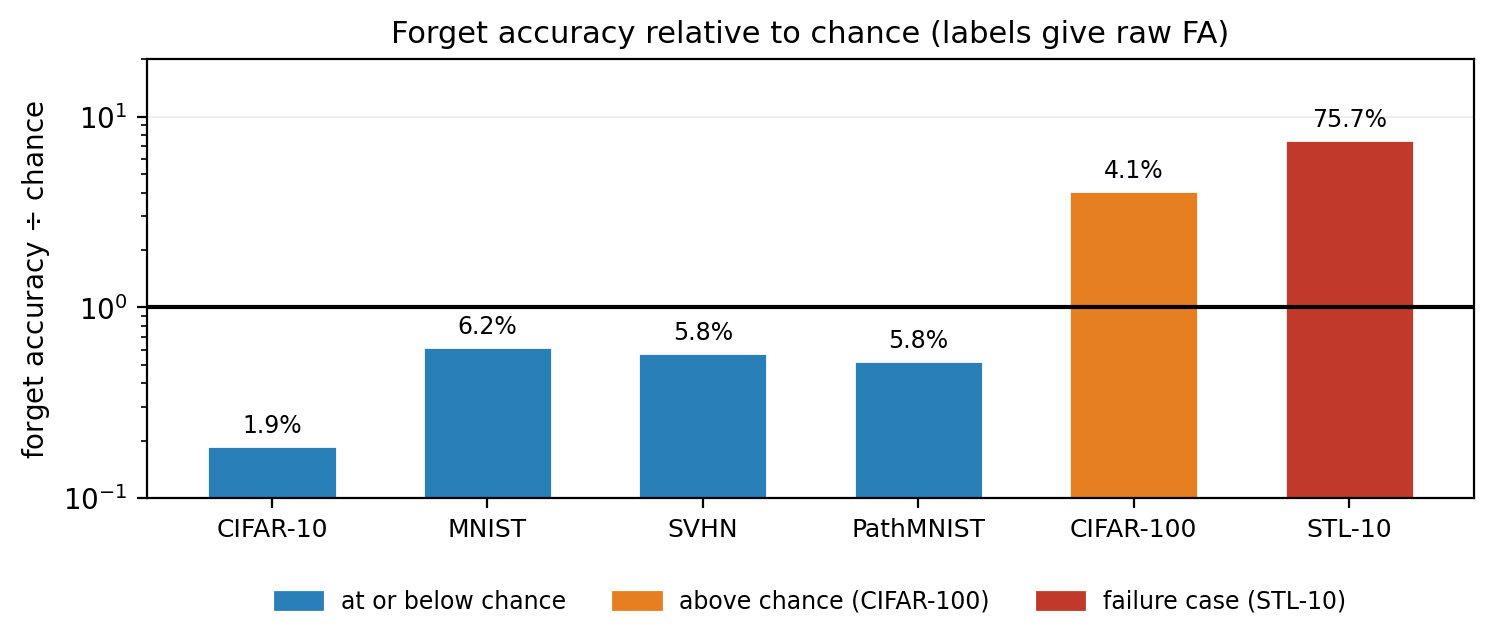
\includegraphics[width=0.86\textwidth]{fig_crossdataset.png}
\caption{\textbf{Forget accuracy relative to the chance level.} Raw forget
accuracy is not comparable across datasets: CIFAR-100's $4.1\%$ is
\emph{above} its $1\%$ chance level while MNIST's $6.2\%$ is \emph{below} its
$10\%$ one. Dividing by $100/K$ puts ``at chance'' at $1.0$ everywhere. Four
datasets sit below chance, CIFAR-100 above it despite a ${\sim}95$pp reduction,
and STL-10 above it at \rev{its 15-epoch cap, though not at 60 epochs}
(\S\ref{sec:crossdataset_stl}).}
\label{fig:crossdataset}
\end{figure}

\paragraph{The projection alone does not unlearn.}
The \emph{projection-only} row is the direct projected-gradient baseline: A-GEM
projection applied to plain gradient ascent, with the KD anchor and the
retain-confusion target removed. It preserves the retain set almost perfectly
($\mathrm{RA} = 99.90\%$), which is what the guarantee promises and all that it
promises---but it stops at $\mathrm{FA} = 18.66\%$, above the $10\%$ chance
level, and halts on the retain-loss budget rather than on the forget target.
Read together with the equal-compute ablation (Table~\ref{tab:ablation}), where
\emph{removing} the projection costs $47.4$pp of retain accuracy, this
delineates the division of labour precisely: the projection supplies retain
safety and nothing else, while the \klr{} objective is what actually drives
forget accuracy to chance. Neither component is sufficient alone, which is the
substantive content of the ablation.

\paragraph{CIFAR-100: scaling to 100 classes.}
Table~\ref{tab:cifar100} gives per-class results (base model TA~$=78.5\%$,
chance $=1\%$). \ours{} reduces FA from ${\sim}99\%$ to a mean of $4.07\%$
(median $1.60\%$) while holding RA at $92.19\%$, with MIA averaging $0.500$.
Eight of nine classes reach FA~$\le 6.8\%$; class~60 is an outlier at $17.8\%$
that does not converge within the 20-epoch budget, and it alone accounts for the
gap between the mean and the median (excluding it, mean FA is $2.35\%$). Unlike
the 10-class datasets, CIFAR-100 does not reach its $1\%$ chance level, so we
report it as a ${\sim}95$pp reduction rather than as forgetting to chance.

\begin{table}[t]
\centering
\caption{\textbf{CIFAR-100 class-level forgetting} (single seed per class,
chance $=1\%$). $^*$Class~60 does not converge within the 20-epoch budget.}
\label{tab:cifar100}
\begin{tabular}{@{}ccccc@{}}
\toprule
Forget class & TA (\%) & FA (\%)$\downarrow$ & RA (\%) & MIA \\
\midrule
10 & 77.23 & 4.20 & 92.84 & 0.485 \\
20 & 76.69 & 1.60 & 92.80 & 0.485 \\
30 & 75.18 & 1.40 & 91.03 & 0.486 \\
40 & 77.19 & 6.80 & 93.14 & 0.506 \\
50 & 76.25 & 0.60 & 92.31 & 0.562 \\
60$^*$ & 76.76 & 17.80 & 92.86 & 0.445 \\
70 & 75.38 & 1.60 & 90.89 & 0.482 \\
80 & 74.95 & 1.00 & 91.51 & 0.553 \\
90 & 75.87 & 1.60 & 92.32 & 0.498 \\
\midrule
\textbf{Mean} & \textbf{76.17} & \textbf{4.07} & \textbf{92.19} & \textbf{0.500} \\
\textbf{Median} & \textbf{76.25} & \textbf{1.60} & \textbf{92.31} & \textbf{0.486} \\
\bottomrule
\end{tabular}
\end{table}

\subsection{Momentum in Detail}\label{app:momentum}

The most direct route to an exact per-step guarantee is to remove momentum, so
that the applied update \emph{is} the projected gradient. Table~\ref{tab:momentum}
shows what that costs. With $\mu=0$ and all else fixed, \ours{} fails to forget
on five of six datasets: FA remains at $95.9\%$ on MNIST, $99.7\%$ on STL-10,
$73.7\%$ on CIFAR-100, and $61.9\%$ on SVHN. Retain accuracy stays high
throughout---but only because the model barely moves; high RA together with high
FA is the signature of a method that preserves retained knowledge by declining
to unlearn.

This is the empirical content of our central methodological claim. A per-step
guarantee stated for the momentum-free update would be exact and
implementation-matched, yet would describe a method that does not unlearn.
Projecting the post-momentum update instead keeps the guarantee exact
\emph{and} recovers forgetting on every dataset where it is attainable.

\begin{figure}[t]
\centering
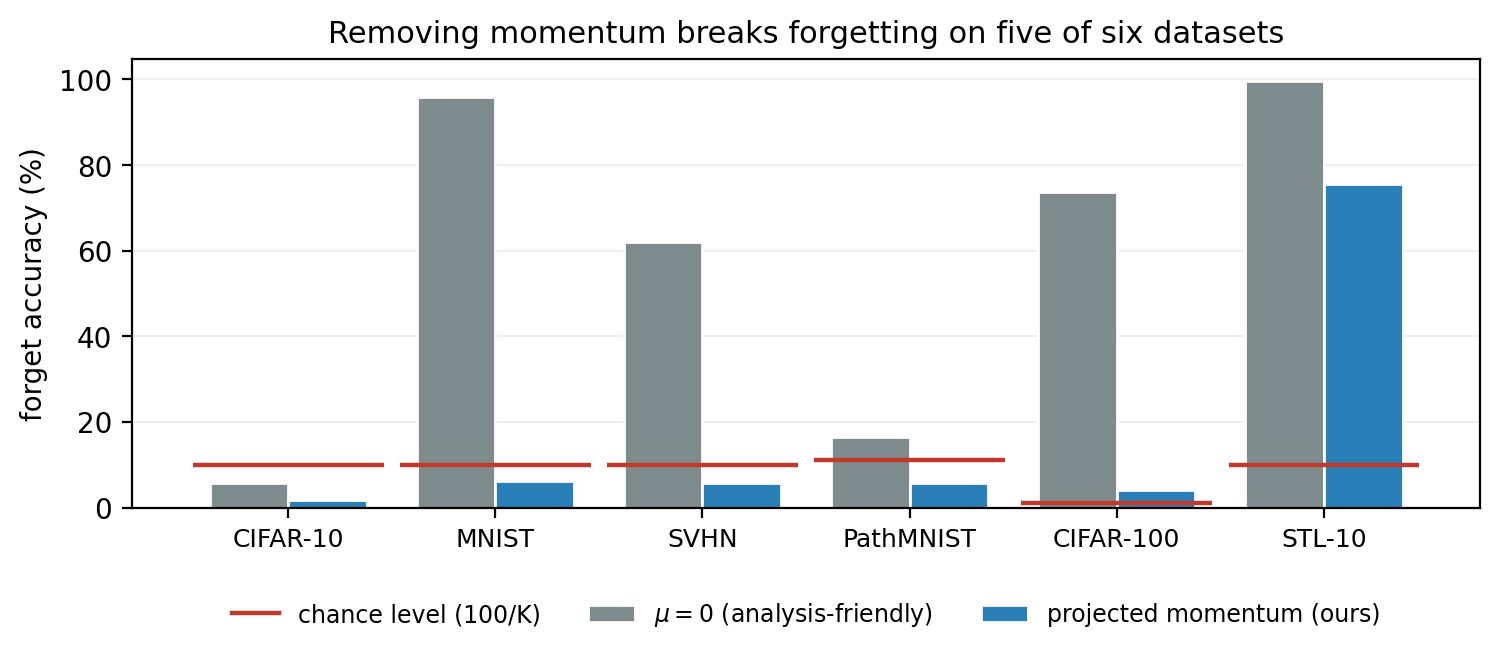
\includegraphics[width=0.86\textwidth]{fig_momentum.png}
\caption{\textbf{Momentum is not incidental.} Forget accuracy with momentum
removed ($\mu=0$, grey) against the projected-momentum update (blue), with each
dataset's chance level in red. The momentum-free configuration---the one for
which an exact guarantee is easiest to state---fails to forget on five of six
datasets. Retain accuracy stays high throughout (Table~\ref{tab:momentum}),
because the model barely moves.}
\label{fig:momentum}
\end{figure}

\paragraph{Is the dependence ours, or the field's?} A natural objection is that
this ablation only tells us something about \ours{}. If every gradient-based
unlearning rule collapses without momentum, the finding is about optimisers and
not about our design; if only ours does, the hard constraint is fragile. We
therefore repeated the ablation across four update rules on the two datasets
where Table~\ref{tab:momentum} shows the largest effect, at \emph{equal compute}
with stopping disabled so that the momentum change is not confounded with step
count (Table~\ref{tab:momentum_rules}).

\begin{table}[t]
\centering
\caption{\textbf{Where the momentum dependence comes from} (equal compute, 12
epochs on MNIST and 15 on SVHN, dual stopping disabled). $\Delta$ is the increase
in forget accuracy when momentum is removed, so larger is more dependent.
Grouping by forget objective separates the rows cleanly; grouping by whether the
projection is used does not.}
\label{tab:momentum_rules}
\begin{tabular}{@{}llcccc@{}}
\toprule
Update rule & Forget objective & Projection & MNIST $\Delta$ & SVHN $\Delta$ & mean \\
\midrule
\ours{}            & $\KL \to p_r$      & yes & $+95.3$ & $+62.4$ & $\mathbf{+78.8}$ \\
\texttt{kl\_uniform} & $\KL \to$ uniform & yes & $+84.9$ & $+56.3$ & $\mathbf{+70.6}$ \\
\addlinespace
projection only    & gradient ascent  & yes & $+16.5$ & $+13.2$ & $+14.8$ \\
gradient ascent    & gradient ascent  & no  & $+11.5$ & $+12.5$ & $+12.0$ \\
\bottomrule
\end{tabular}
\end{table}

Every rule degrades without momentum, including plain gradient ascent, which
uses no projection at all---so the dependence is not an artefact of operating
under a hard per-step constraint. But the rules do not degrade equally, and the
grouping is informative. The two KL-based objectives lose $70$--$79$pp of forget
accuracy on average, the two gradient-ascent objectives $12$--$15$pp: a factor
of $5.6$. Meanwhile the like-for-like comparison that isolates the
projection---gradient ascent with it ($+14.8$) against gradient ascent without
it ($+12.0$)---differs by only $2.8$pp.

The momentum dependence therefore belongs to the \emph{forget objective}, not to
the projection. The reason is visible in the objective itself: $\KL(p_\theta(x_f)
\| p_r)$ is bounded and its gradient vanishes as $p_\theta \to p_r$, so the
per-step signal is small and the $1/(1-\mu) = 10\times$ amplification that
momentum supplies (Lemma~\ref{lem:vel}) is what makes progress possible at
all. Gradient ascent maximises an unbounded loss and needs no such
amplification, which is also why it damages the retained model.

This sharpens rather than weakens the section's claim. The point was never that
momentum is uniquely important to \ours{}; it is that the guarantee must be
stated for the update the optimiser applies, and any method whose objective
requires momentum inherits that requirement. A momentum-free analysis is
convenient for exactly the objectives that cannot afford to be momentum-free.

\subsection{Auditing the Guarantee at Step Level}\label{sec:alignment}

We log every gradient step of a CIFAR-10 class-0 run (120 steps) and check
Theorem~\ref{thm:retain_safety} directly rather than assuming it.

\begin{itemize}
\item \textbf{The constraint is active, not vacuous.} All $120/120$ steps have
$\langle v_t,\gr\rangle < 0$, so the projection fires at every step. Projection
here is not an occasional correction: without it, every step would increase
retain loss to first order.
\item \textbf{The guarantee holds.} After projection,
$\langle u_t,\gr\rangle \ge 0$ at every step to floating-point precision. The
largest relative violation is
$\langle u_t,\gr\rangle/(\|u_t\|\|\gr\|) = -7.4\times 10^{-7}$, against a
float32 accumulation scale of ${\sim}4\times 10^{-4}$ for sums over 11.2M
parameters; the mean relative alignment is positive
($+2.2\times 10^{-8}$). The implied worst-case first-order retain increase is
$3.1\times 10^{-7}$, three orders of magnitude below the observed per-step
retain-loss fluctuation ($1.8\times 10^{-4}$). We therefore state the guarantee
as holding to float32 precision, and recommend float64 accumulation for the
inner products in reference implementations.
\item \textbf{The norm bound is respected.} $\|u_t\|$ reaches a maximum of
$9.16$ against the theoretical bound $c/(1-\mu)=10$, with mean $7.35$---close to
but never exceeding the bound, confirming both that the bound is tight and that
momentum's amplification is being realised.
\item \textbf{Retain loss is controlled.} The mean per-step change in mini-batch
retain CE is $-7.9\times 10^{-5}$ (i.e.\ decreasing), with a maximum single-step
increase of $+1.05\times 10^{-3}$, consistent with the $O(\eta^2)$ term of
Eq.~\ref{eq:thm1}.
\end{itemize}

\subsection{BatchNorm Recalibration in Detail}\label{app:bn}

Table~\ref{tab:gn} reports \ours{} with a GroupNorm backbone across datasets.
GroupNorm keeps forgetting intact on four of five datasets at a modest TA cost
(e.g.\ CIFAR-10 $84.16\%$ vs $86.13\%$), while removing the BN-recalibration
mechanism by construction, since there are no batch statistics to recalibrate.
STL-10 is under-trained under GroupNorm as it is under BN, at \rev{its epoch cap}
(\S\ref{sec:crossdataset_stl}).

\begin{table}[t]
\centering
\caption{\textbf{\ours{} with a GroupNorm backbone} (3-seed means). GroupNorm
removes the BN-recalibration vulnerability structurally. $^*$STL-10 is under-trained under
both backbones.}
\label{tab:gn}
\begin{tabular}{@{}lcccc@{}}
\toprule
\textbf{Dataset} & \textbf{TA} & \textbf{FA}$\downarrow$ & \textbf{RA} & \textbf{MIA} \\
\midrule
CIFAR-10    & 84.16 & 3.44 & 99.23 & 0.478 \\
MNIST       & 90.17 & 5.84 & 99.31 & 0.500 \\
SVHN        & 87.99 & 3.46 & 95.49 & 0.581 \\
STL-10$^*$  & 83.92 & 97.60 & 92.95 & 0.552 \\
PathMNIST   & 72.00 & 2.71 & 95.97 & 0.583 \\
\bottomrule
\end{tabular}
\end{table}

Table~\ref{tab:bnrecal} reports the diagnostic itself. The operator is
\texttt{torch.optim.swa\_utils.update\_bn} applied to the retain set: it resets
every BatchNorm buffer, sets the momentum to \texttt{None} so that PyTorch
accumulates a cumulative rather than exponential average, and runs forward
passes with no backward pass and no weight update. The resulting statistics are
therefore the exact retain-set statistics, independent of the pre-attack buffers
and idempotent in the data. We verify after every run that all learnable
parameters are bit-identical, so nothing but the buffers can have changed. Then
$\Delta F = \mathrm{post} - \mathrm{pre}$ separates weight-level forgetting
($\Delta F \approx 0$) from forgetting mediated by batch statistics
($\Delta F \gg 0$). We also report a weaker variant---forward passes in
\texttt{train} mode under the default exponential average, which is what an
earlier version of this work used---and the two agree to within $1.2$pp on every
row, and to $0.02$pp on the \ours{} row that carries the finding, so the choice
of estimator is not what drives the result. All
accuracies here are measured under deterministic (test-time) transforms; leaving
training augmentation active perturbs individual rows by several points.



\paragraph{The vulnerability is ours, not the field's---in our reproductions.}
The baseline rows matter more than \ours{}'s. Every one of them is unaffected by
recalibration---the largest movement is SCRUB's $-3.6$pp, in the direction of
\emph{more} forgetting---and so is the base model, which is the control that
matters: recalibrating a normally trained network changes nothing, because its
statistics already agree with its weights. Only \ours{} carries a mismatch.
$\Delta F = +98.4$pp means the attack does not merely degrade the unlearning but
\emph{undoes} it: forget accuracy returns to $99.7\%$ and test accuracy to
$92.9\%$\rev{---the values recalibration gives the base model itself ($99.8\%$
and $92.9\%$)}---without a single weight being modified. On a BatchNorm backbone, what \ours{} produces is not an
unlearned model but an unlearned model's statistics.

We qualify the first half of that heading deliberately. \rev{Concurrent work
\citep{kalani2026batchnorm} reports large recoveries for SalUn ($+62.1$pp) and
Bad Teacher ($+78.2$pp) under their reference implementations, where we measure
none. We ran the identical operator, so the disagreement is not in the attack
but in how the unlearned checkpoints were produced. Our implementations end
every epoch with a full pass over retained data in train mode, which recomputes
the running statistics before the checkpoint is saved; \citet{kalani2026batchnorm}
run Bad Teacher's BatchNorm in eval mode, and find that SalUn's recovery
disappears once at least a quarter of each unlearning batch is retained data.}
Our claim is therefore that the vulnerability is \ours{}-specific \emph{among
the checkpoints we trained}, not that these baselines are immune in general.

We attribute it, tentatively, to the interaction between our own design choice
and BatchNorm. \ours{} freezes the normalisation statistics during unlearning so
that class-homogeneous forget batches cannot corrupt them; the weights therefore
adapt against \emph{fixed} statistics, and the resulting decision boundary is
valid only for those statistics. Methods that let the statistics move during
unlearning never build that dependence. Freezing BatchNorm is thus necessary but
not sufficient: it prevents the statistics from manufacturing apparent
forgetting, and simultaneously makes the weights depend on them.
\added{Section~\ref{sec:bn_robust} puts this attribution to an interventional
test: keeping the statistics consistent with the weights throughout unlearning
removes the vulnerability.}

The GroupNorm backbone removes the mechanism by construction---there are no batch
statistics to recalibrate---at a cost of $2.0$pp of test accuracy
(Table~\ref{tab:gn}). The ViT-B/16 backbone
(\S\ref{sec:vit}) does the same for a different reason: LayerNorm normalises
per example at inference and keeps no running statistics either. Two
architectures with unrelated designs are both outside the operator's reach, and
both unlearn properly, which locates the defect in the normalisation scheme
rather than in gradient projection.

We state the limit of that plainly: neither backbone \emph{resists} the attack,
because the attack is undefined on them. This is a design change, not
demonstrated robustness, and a method that must avoid BatchNorm to be safe is
constrained in a way the guarantee itself does not capture. What the two rows do
establish is that the defect is separable from \ours{}'s mechanism---it is a
property of freezing statistics that a normalisation layer keeps, and it
disappears wherever there are no such statistics. \added{The next subsection
removes the constraint itself: it keeps BatchNorm, and makes \ours{} robust to
the attack rather than outside its reach.}

\begingroup\color{revised}% ---- new subsection: everything to \endgroup is added
\subsection{BN-robust \ours{} in Detail}\label{app:bn_robust}

The diagnosis above points at its own remedy: if the weights learn to forget
against statistics that are allowed to go stale, the statistics should never be
stale. BN-robust \ours{} makes three changes to Algorithm~\ref{alg:excise}
(Figure~\ref{fig:bnrobust_mech}). It leaves the update rule untouched, \rev{so
Theorem~\ref{thm:retain_safety} holds at every step for the retain objective
under the statistics in force during that step; the recalibration between steps
is not covered by it}.
\begin{enumerate}
\item \emph{Track the weights.} Before every step the BatchNorm statistics are
recomputed, $\phi \leftarrow R(\theta, B_r)$, with the attacker's own operator
$R$ (\texttt{update\_bn}) on a fresh sample $B_r$ of $512$ retain images. The
step's forward and backward passes then run under statistics consistent with the
current weights. Forget batches still never touch the statistics: this keeps
the half of freezing that was right and drops the half that was wrong.
\item \emph{Ship consistent statistics.} After the last step,
$\phi \leftarrow R(\theta_T, \Dr)$ on the whole retain set under test-time
transforms---exactly what the attacker computes.
\item \emph{Stop on the forget accuracy that ships.} The stopping rule of
\S\ref{sec:stopping} reads FA under $R(\theta, \Dr)$ with test-time transforms,
not under the in-loop statistics. If the target is not met within the epoch
budget, the epoch with the lowest such FA inside the retain budget is shipped
instead of the last one.
\end{enumerate}
\begin{figure}[t]
\centering\color{revised}
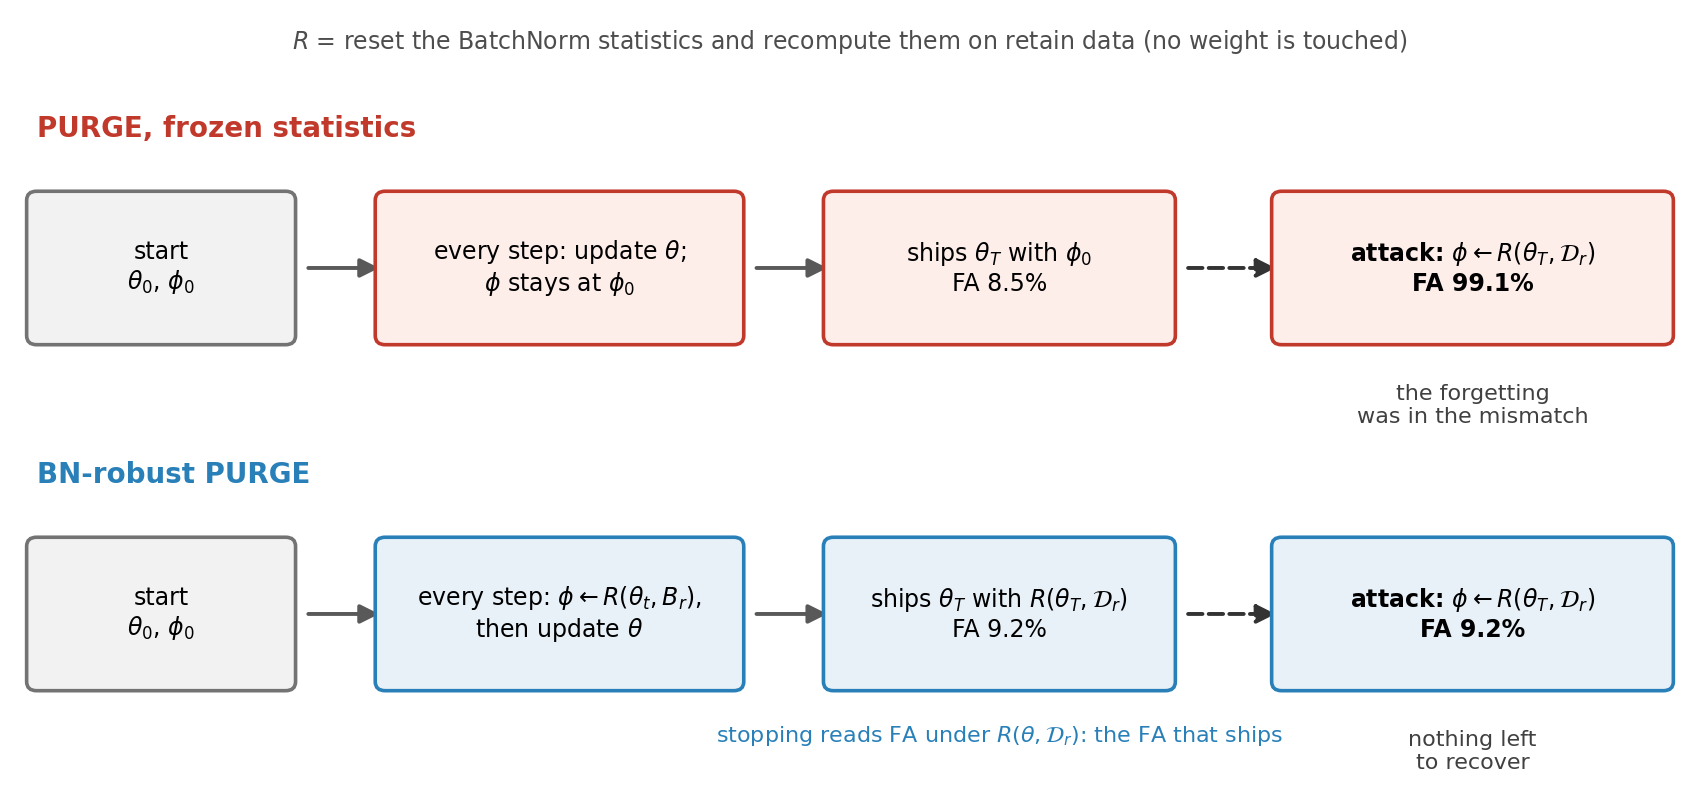
\includegraphics[width=\textwidth]{fig_bnrobust_mechanism.png}
\caption{\added{\textbf{What BN-robust \ours{} changes.} $R$ resets the BatchNorm
statistics and recomputes them on retain data without touching a weight. With
frozen statistics the forgetting lives in the mismatch between $\theta_T$ and
$\phi_0$, and the attack removes it; BN-robust ships statistics consistent with
its weights, so the attack has nothing to recover. Forget accuracies are
CIFAR-10 class~0, means over three seeds (Table~\ref{tab:bnrobust}).}}
\label{fig:bnrobust_mech}
\end{figure}

Because $R$ is idempotent, change~2 makes the attack a no-op on the shipped model
by construction, so $\Delta F = 0$ is not by itself evidence here. The question
this variant must answer is whether FA is still low once $\phi$ cannot be
stale. Two of the tests below are not no-ops by construction: the
exponential-average operator, and recalibration on data other than the retain
set.

Change~3 is not cosmetic. Without it, the FA that triggers stopping is read under
the in-loop statistics---a few hundred augmented images, one step behind---on
augmented forget images. On CIFAR-10 that reading falls short of the shipped FA
by between $-1.0$ and $+9.0$pp depending on the class, and runs stopped at
``FA $\le 10\%$'' shipped at $7.2$--$16.7\%$ (Figure~\ref{fig:bnrobust_stop}). With change~3 the shipped FA meets
the target, and the seed-to-seed spread on class~0 falls from $1.90$ to
$0.08$pp (Table~\ref{tab:bnrobust}). The stopping check need not use the whole
retain set. Computing it on $10{,}240$ images reproduced every stopping decision
of the full check on all three seeds and cut wall-clock by $16\%$; the shipped
statistics still use the full set.

\begin{figure}[t]
\centering\color{revised}
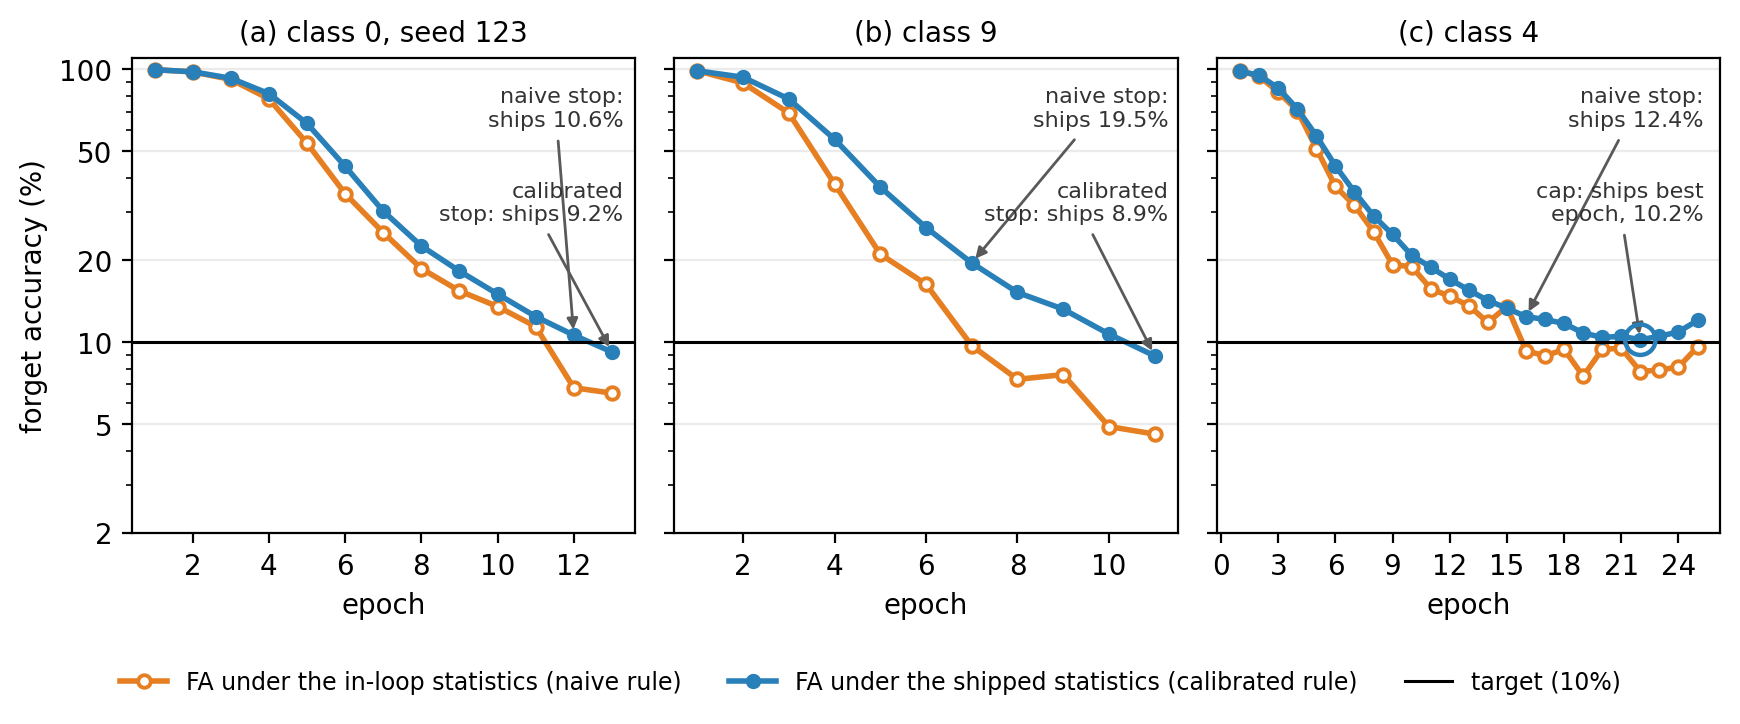
\includegraphics[width=\textwidth]{fig_bnrobust_stopping.png}
\caption{\added{\textbf{Why stopping must be calibrated.} Forget accuracy per epoch
under the in-loop statistics (what naive stopping reads) and under the
statistics that ship (what calibrated stopping reads); log scale. The in-loop
reading runs below the shipped one, so a naive rule stops early and ships above
chance: (a)~one epoch early on class~0, (b)~four epochs early on class~9,
shipping $19.5\%$ instead of $8.9\%$. (c)~On class~4 the shipped FA plateaus just
above $10\%$ and the run reaches the epoch cap; the best-epoch rule ships epoch~22
($10.2\%$) rather than the last ($12.0\%$).}}
\label{fig:bnrobust_stop}
\end{figure}

These experiments were run after the checkpoints behind
Table~\ref{tab:bnrecal} became unavailable. They use an earlier CIFAR-10 base
(test accuracy $93.97\%$, against $95.5\%$ there), a GroupNorm base retrained for
$100$ rather than $200$ epochs ($91.89\%$), and a retrained MNIST base
($99.59\%$). Their absolute numbers are therefore not comparable row for row
with the rest of \S\ref{sec:experiments}; every comparison below is between arms
that share a base.



\paragraph{It survives the attack it was built against, and two it was not.}
Calibrated BN-robust forgets class~0 to $9.19\%$ and stays at $9.18\%$ under
recalibration (Figure~\ref{fig:bnrobust_attack}a), while the frozen configuration
returns to $99.12\%$ with test accuracy back at $94.1\%$---the original model. The exponential-average
operator, which is not idempotent and therefore not a no-op here, moves
BN-robust by at most $+0.3$pp. Nor does robustness depend on the attacker using
the retain set. On the naive-stopping checkpoints, recomputing the statistics
on the full training set, forget class included, or on the test set---data
BN-robust never trained under---moves its FA by $-1.0$ to $-1.2$pp, towards more
forgetting, while the frozen configuration still recovers to $97.4\%$ and
$97.3\%$ (Figure~\ref{fig:bnrobust_attack}b).

\paragraph{Every class, and a second dataset.}
On all ten CIFAR-10 classes (seed~$42$; Table~\ref{tab:app_bnrobust} and
Figure~\ref{fig:app_bnrobust}), the
frozen configuration recovers to $94.7$--$99.3\%$ under the attack, while
BN-robust's FA moves by at most $0.06$pp under either stopping rule. With
calibrated stopping every class ships between $6.7\%$ and $10.2\%$, inside three
standard errors of chance ($11.3\%$ for $5{,}000$ images); with naive stopping,
five of the ten did not. One class needed the fallback. Class~4 hovered at
$10.2$--$10.9\%$ for six epochs without crossing $10\%$ and reached the epoch
cap, and the rule shipped its best epoch ($10.2\%$) rather than the last
($11.9\%$, with retain accuracy $1.4$pp lower). On MNIST, over three seeds, the
frozen configuration's forgetting is undone completely ($0.00\% \to 99.97\%$,
with test accuracy back to $99.56\%$ against the base's $99.59\%$), and
BN-robust holds ($3.78\% \to 3.87\%$, test accuracy $90.10\%$).

\paragraph{What it costs, and why it is slower.}
Against the frozen configuration, BN-robust gives up $1.8$pp of retain accuracy
and $0.9$pp of test accuracy and takes about seven times the wall-clock, most of
it because it needs $13$ epochs instead of $2$. We read the slower forgetting as
the substance rather than the overhead. The frozen configuration reaches its
target in two epochs largely through the statistics mismatch, which the attack
shows is not forgetting at all; once the statistics track the weights, the
forgetting has to happen in the weights. BN-robust's test accuracy, $84.30\%$,
is close to the $84.6\%$ expected from removing one class of ten from a
$93.97\%$ model. Against GroupNorm, BN-robust keeps $1.2$pp more test accuracy,
mostly because it can start from the stronger BatchNorm base, and it needs
neither a change of architecture nor a retrained base model.
Membership-inference AUROC stays between $0.48$ and $0.52$ for every unlearned
row.

\paragraph{What it does and does not establish.}
Unlike GroupNorm or a transformer, this is robustness rather than immunity by
construction: the attack is defined on the model, runs, and finds nothing to
recover. It is robustness to one attack, though. BN-robust changes only how the
normalisation statistics are maintained, so it does nothing against attacks that
modify the weights, such as fine-tuning recovery (\S\ref{sec:limitations}), and
we have tested it on two datasets rather than six. Within that scope, \ours{} no
longer has to choose between BatchNorm and its forgetting: BN-robust \ours{},
\ours{} with GroupNorm, and \ours{} on a transformer are all configurations we
would deploy.
\endgroup% ---- end of the added subsection

\subsection{A Transformer Backbone}\label{sec:vit}

Every result so far uses ResNet-18, so the projection has only ever been applied
to a convolutional network. We repeat CIFAR-10 class~0 on ViT-B/16 under the
identical algorithm, with representation erasure disabled as everywhere else,
over three seeds.

\begin{table}[t]
\centering
\caption{\textbf{ViT-B/16 against ResNet-18}, same algorithm and forget targets
as Table~\ref{tab:cross}\rev{; the ViT runs check forget accuracy every step.
Chance is $10\%$ on CIFAR-10 and $1\%$ on CIFAR-100. The projection fires on
$98$--$100\%$ of steps, as it does on ResNet-18.}}
\label{tab:vit}
\begin{tabular}{@{}lcccc@{}}
\toprule
Backbone & TA & FA$\downarrow$ & RA & MIA \\
\midrule
\multicolumn{5}{@{}l}{\rev{\emph{CIFAR-10, class~0, three seeds}}} \\
ResNet-18 (Table~\ref{tab:cross}) & $86.13 \pm 0.02$ & $1.87 \pm 0.25$ & $100.00 \pm 0.00$ & $0.529$ \\
ViT-B/16                          & $87.05 \pm \rev{0.09}$ & $9.71 \pm \rev{0.27}$ & $\phantom{0}97.55 \pm \rev{0.10}$ & $0.453$ \\
\midrule
\multicolumn{5}{@{}l}{\rev{\emph{CIFAR-100, classes $10,\dots,90$, one seed each, 20-epoch cap}}} \\
\rev{ResNet-18 (Table~\ref{tab:cross})} & \rev{$76.17 \pm 0.86$} & \rev{$4.07 \pm 5.51$} & \rev{$92.19 \pm 0.84$} & \rev{$0.500$} \\
\rev{ViT-B/16} & \rev{$81.97 \pm 0.66$} & \rev{$24.00 \pm 23.16$} & \rev{$91.86 \pm 0.73$} & \rev{$0.435$} \\
\bottomrule
\end{tabular}
\end{table}

\rev{On CIFAR-10} forgetting transfers: FA reaches $9.71\%$, below the $10\%$
chance level, with retain accuracy at $97.55\%$ and test accuracy slightly
\emph{above} the ResNet-18 result. The gap in FA against ResNet-18's $1.87\%$ is not a weaker
result but a different stopping point---both runs use $\tau_F = 10\%$, and
the ViT run halts as soon as it crosses that threshold (epoch~3, mid-epoch),
whereas the ResNet-18 run overshoots it. \S\ref{sec:experiments} shows that
overshoot is an artifact of check granularity rather than a property of either
backbone.

\rev{On CIFAR-100 it does not transfer within the same 20-epoch cap. On the nine
classes of Table~\ref{tab:cross}, ViT-B/16 ends with FA between $4.0\%$ and
$82.0\%$ (mean $24.0\%$) against a $1\%$ chance level, so no class reaches
chance, where ResNet-18 ends at $4.07\%$ and reaches chance at 60 epochs.
Retain accuracy ($91.9\%$) matches ResNet-18's. We have not tested whether a
longer budget closes the gap, as it does for ResNet-18; until then the
transformer result holds for CIFAR-10 only.}

Two things follow. First, the conflict the projection resolves is not an artifact
of convolutional architectures: the projection fires on $99$--$100\%$ of steps
here as well, so forget and retain gradients oppose one another just as
routinely in a transformer. Second, and more usefully,
ViT normalises with LayerNorm, which computes statistics per example at
inference and stores none. It is therefore outside the reach of the
recalibration operator of \S\ref{sec:bn_results} for the same structural reason
as GroupNorm, but by way of a completely different architecture---which is what
makes the pair informative rather than merely repetitive.

\subsection{Component Ablation}\label{sec:ablation}

A component ablation run in the deployed configuration is uninformative here,
and the reason is instructive. Under the projected-momentum optimiser every
variant reaches the forget-accuracy target inside the first check interval, so
dual stopping halts them all after one epoch and each looks equally good: in the
upper half of Table~\ref{tab:ablation}, removing the projection costs
$0.09$pp of retain accuracy. That number is an artefact of stopping, not a
measurement of what the projection does.

We therefore also run every variant at \emph{equal compute}, with stopping
disabled throughout (lower half). The picture inverts.

\begin{table}[t]
\centering
\caption{\textbf{Component ablation} (CIFAR-10 class~0, seed 42). Upper: the
deployed configuration, where dual stopping halts every variant after one epoch.
Lower: equal compute, 15 epochs, stopping disabled for all variants---the same
comparison without the stopping confound. \texttt{+rep} and \texttt{+gate}
re-introduce the two components removed in \S\ref{sec:method}.}
\label{tab:ablation}
\begin{tabular}{@{}llcccc@{}}
\toprule
& Variant & TA & FA & RA & MIA \\
\midrule
\multirow{7}{*}{\rotatebox{90}{\emph{stopping on}}}
 & full \ours{}      & $86.10$ & $2.14$ & $100.00$ & $0.528$ \\
 & $-$KD             & $85.56$ & $0.80$ & $99.99$  & $0.516$ \\
 & $-$projection     & $84.87$ & $0.78$ & $99.91$  & $0.513$ \\
 & selective-layer   & $86.26$ & $3.26$ & $100.00$ & $0.528$ \\
 & $+$rep            & $86.10$ & $2.14$ & $100.00$ & $0.528$ \\
 & $+$gate           & $86.10$ & $2.14$ & $100.00$ & $0.528$ \\
 & $-$stopping       & $85.71$ & $0.00$ & $99.98$  & $0.472$ \\
\midrule
\multirow{6}{*}{\rotatebox{90}{\emph{equal compute}}}
 & full \ours{}      & $85.70$ & $0.00$ & $99.98$  & $0.472$ \\
 & $-$KD             & $85.66$ & $0.00$ & $99.94$  & $0.475$ \\
 & $-$projection     & $\mathbf{44.37}$ & $0.00$ & $\mathbf{52.55}$ & $0.436$ \\
 & selective-layer   & $85.76$ & $0.00$ & $99.99$  & $0.469$ \\
 & $+$rep            & $85.74$ & $0.00$ & $99.98$  & $0.473$ \\
 & $+$gate           & $87.16$ & $19.28$ & $100.00$ & $0.539$ \\
\bottomrule
\end{tabular}
\end{table}

\paragraph{The projection is what makes unlearning survivable.}
At equal compute, removing it costs $41.3$pp of test accuracy and
$47.4$pp of retain accuracy: the model collapses to $44.4/52.6$ against
$85.7/99.98$ for the full method. This is the empirical counterpart of
Theorem~\ref{thm:retain_safety}, and it is a far larger effect than the
stopping-confounded comparison suggests. Note also that the two rows disagree
about the \emph{sign} of the conclusion---one reports the projection as
costless, the other as indispensable---which is why we report both rather than
whichever is more favourable.

\paragraph{KD contributes little once compute is equalised.}
Removing the distillation anchor changes retain accuracy by $0.04$pp at equal
compute. We previously attributed several points of retain accuracy to it; that
is not supported here, and we no longer claim it.

\paragraph{The removed components stay removed.}
Re-introducing representation erasure reproduces the full method to within
$0.04$pp on every metric, and re-introducing the entropy gate leaves forget
accuracy at $19.3\%$---above the $10\%$ chance level, i.e.\ it prevents the
method from forgetting. Both were dropped in \S\ref{sec:method} on the strength
of an ablation run under the previous implementation; this re-run confirms the
decision under the current one.

\subsection{How Hard Must the Constraint Be?}\label{sec:strength}

Theorem~\ref{thm:separation}(iv) argues that a soft conflict penalty biases the
update without excluding retain-harming steps, and that only a hard constraint
makes them unreachable. That is an argument about feasible sets; here we measure
what it costs in practice. We interpolate the projection with a strength
parameter $s$: at each conflicting step the update becomes
$u_t = v_t - s\,\frac{\langle v_t,\gr\rangle}{\|\gr\|^2}\gr$, so
\begin{equation}\label{eq:strength}
\langle u_t, \gr\rangle \;=\; (1-s)\,\langle v_t, \gr\rangle .
\end{equation}
At $s=0$ nothing is corrected; at $s=1$ this is \ours{}. Every intermediate
value is a soft penalty---it shrinks the conflicting component without removing
it---and by Eq.~\ref{eq:strength} it leaves $\langle u_t,\gr\rangle<0$ whenever
the raw update conflicts. All other settings are held fixed, and stopping is
disabled so that every variant sees the same compute.

\begin{table}[t]
\centering
\caption{\textbf{Projection strength} (CIFAR-10 class~0, equal compute, stopping
disabled). $s=0$ applies no correction, $s=1$ is the full hard constraint.
Forget accuracy is $0.0\%$ throughout, so the runs differ only in collateral
damage.}
\label{tab:strength}
\begin{tabular}{@{}lccccc@{}}
\toprule
$s$ & residual conflict & TA & FA & RA & MIA \\
\midrule
$0.00$ & $1.00\,\langle v_t,\gr\rangle$ & $44.35$ & $0.0$ & $52.54$ & $0.436$ \\
$0.25$ & $0.75\,\langle v_t,\gr\rangle$ & $67.84$ & $0.0$ & $81.35$ & $0.497$ \\
$0.50$ & $0.50\,\langle v_t,\gr\rangle$ & $78.03$ & $0.0$ & $92.75$ & $0.510$ \\
$0.75$ & $0.25\,\langle v_t,\gr\rangle$ & $82.99$ & $0.0$ & $98.24$ & $0.509$ \\
$1.00$ & $\mathbf{0}$ & $\mathbf{85.71}$ & $0.0$ & $\mathbf{99.98}$ & $0.472$ \\
\bottomrule
\end{tabular}
\end{table}

\begin{figure}[t]
\centering
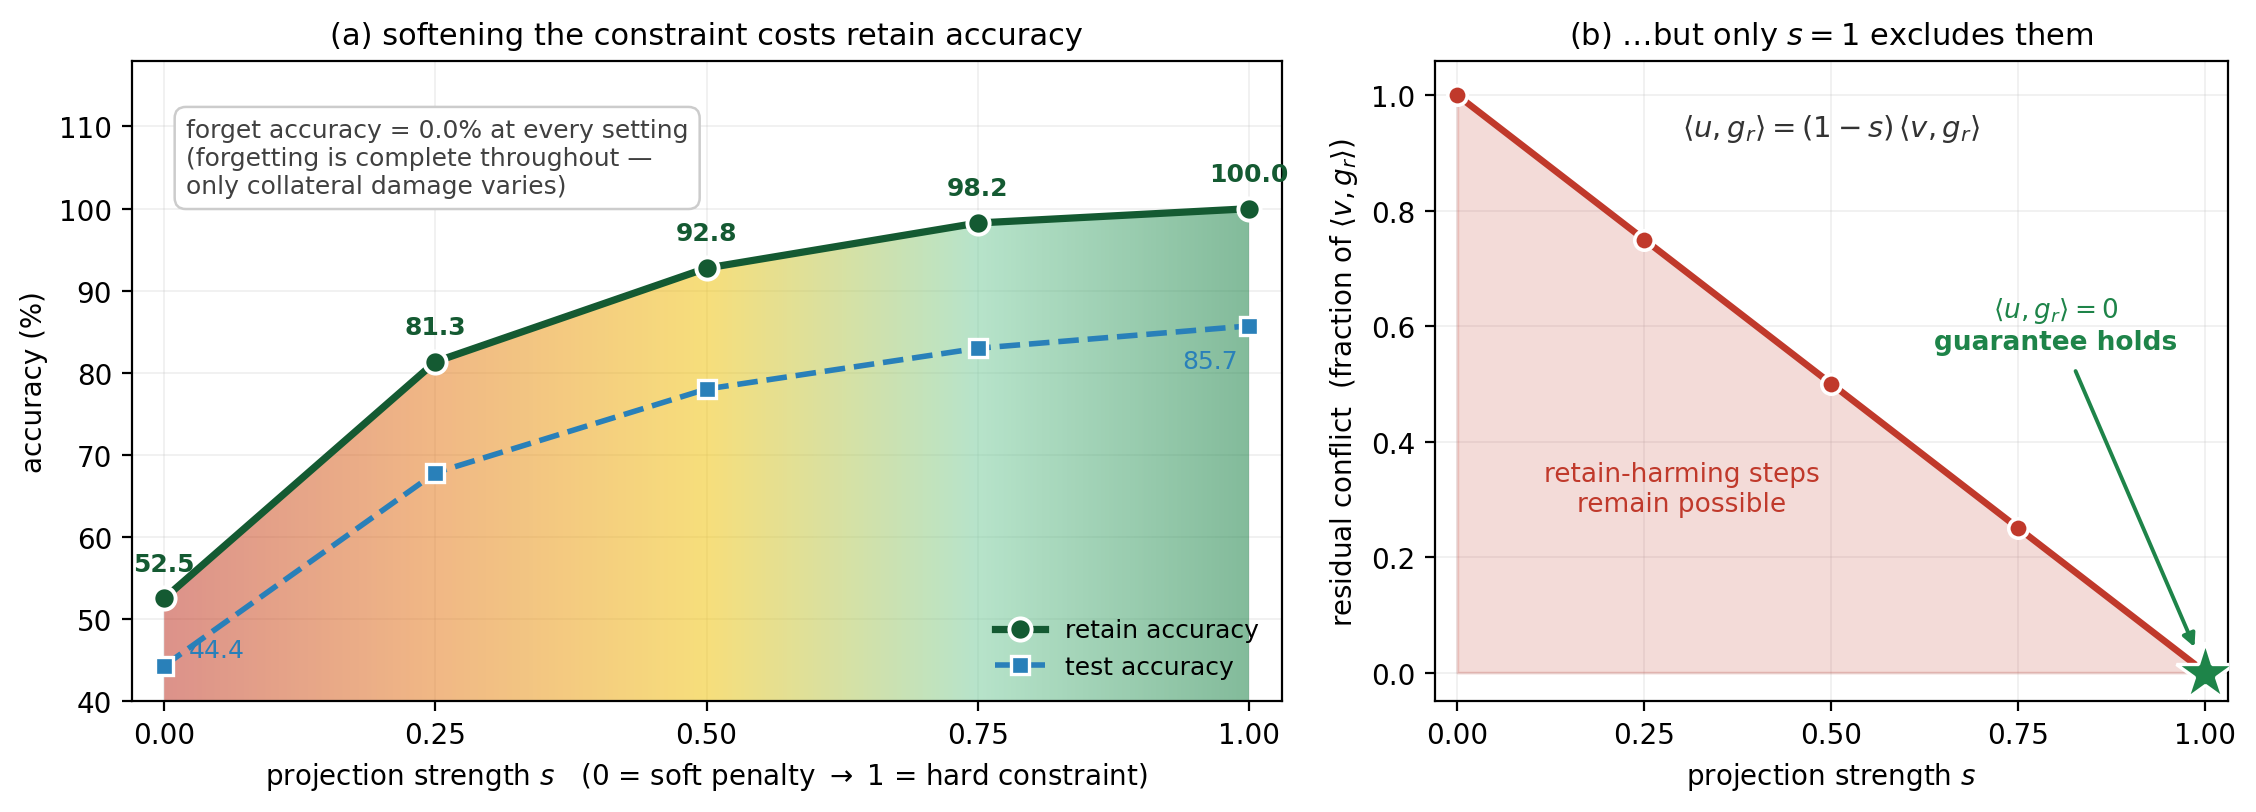
\includegraphics[width=\textwidth]{fig_strength.png}
\caption{\textbf{Hardening the constraint recovers retain accuracy
continuously, but only the endpoint carries the guarantee.}
\textbf{(a)}~Retain and test accuracy against projection strength; forget
accuracy is $0.0\%$ at every setting, so the runs differ only in collateral
damage. \textbf{(b)}~Residual conflict $(1-s)$: retain-harming steps remain
reachable for every $s<1$ and are excluded only at $s=1$. The empirical
difference between $s=0.75$ and $s=1$ is $1.7$pp of retain accuracy; the
difference in what can be proved is categorical.}
\label{fig:strength}
\end{figure}

\paragraph{Softening is expensive, and monotonically so.}
Retain accuracy falls from $99.98\%$ at $s=1$ to $52.54\%$ at $s=0$, and test
accuracy from $85.71\%$ to $44.35\%$, monotonically in between. Because forget
accuracy is $0.0\%$ at every setting, this is not a privacy--utility trade-off:
all five runs forget equally, and they differ only in how much of the retained
model they destroy on the way. The $s=0$ row reproduces the equal-compute
$-$projection ablation of Table~\ref{tab:ablation} from an independent
direction.

\paragraph{The curve is gradual, which we take as a limitation of the empirical
argument.} Most of the benefit arrives early---$s=0.25$ already recovers
$28.8$pp of retain accuracy, while the final quarter, $s=0.75\to1$, is worth
$1.7$pp. A soft penalty tuned near $s=0.75$ therefore performs almost as well as
the hard constraint on these metrics, and we do not claim otherwise. What it
does not do is satisfy Eq.~\ref{eq:strength} with equality: at $s=0.75$ a
quarter of every conflict survives into the applied update, so
$\langle u_t,\gr\rangle<0$ on conflicting steps and no per-step statement can be
made. The case for $s=1$ is therefore not that the last $1.7$pp is large, but
that it is the only setting about which anything can be proved---which is the
whole content of Theorem~\ref{thm:retain_safety}.

\paragraph{Relation to soft conflict-resolution methods.}
This is a controlled test of the mechanism that separates \ours{} from the
closest prior work \citep{patel2025learning}, not a comparison with that method:
it varies our own projection rather than reimplementing theirs, and their
penalty acts on the objective rather than on the update. What it establishes is
the general shape of the trade---that discouraging conflict helps in proportion
to how much of it is removed, and that removing all of it is what converts an
empirical tendency into a guarantee. A like-for-like comparison remains future
work (\S\ref{sec:limitations}).

\subsection{Privacy--Utility Frontier and Robustness Diagnostics}\label{sec:sweeps}

We sweep the two tolerances of Eq.~\ref{eq:problem} independently on CIFAR-10
class~0 (Table~\ref{tab:sweeps}). The results are asymmetric: one tolerance is
inert because the projection has already done its work, while the other is
genuinely active but was hidden by how coarsely we measured it.

\begin{table}[t]
\centering
\caption{\textbf{Tolerance sweeps} (CIFAR-10 class~0). Sweep~A varies the
retain-loss budget $\alpha$ at fixed $\tau_F = 10\%$; Sweeps~B and B$'$ vary
the forget-accuracy target $\tau_F$ at fixed $\alpha = 5$, checking forget
accuracy every 50 batches and every step respectively. $\alpha$ is inert. So is
$\tau_F$ under the coarse check---but only because forget accuracy crosses
the whole range between two consecutive checks; measured per step, it tracks the
requested tolerance across a $29$pp range.}
\label{tab:sweeps}
\begin{tabular}{@{}lccccc@{}}
\toprule
\multicolumn{2}{@{}l}{Sweep A: $\alpha$} & TA & FA & RA & MIA \\
\midrule
& $1.5$    & $86.10$ & $1.88$ & $100.00$ & $0.530$ \\
& $2$      & $86.10$ & $1.88$ & $100.00$ & $0.530$ \\
& $3$      & $86.10$ & $1.88$ & $100.00$ & $0.530$ \\
& $5$      & $86.10$ & $1.88$ & $100.00$ & $0.530$ \\
& $10$     & $86.10$ & $1.88$ & $100.00$ & $0.530$ \\
& $9999$   & $86.10$ & $1.88$ & $100.00$ & $0.530$ \\
\midrule
\multicolumn{2}{@{}l}{Sweep B: $\tau_F$, check every 50 batches} & TA & FA & RA & MIA \\
\midrule
& $1\%$    & $85.75$ & $\phantom{0}0.28$ & $100.00$ & $0.521$ \\
& $5\%$    & $86.10$ & $\phantom{0}1.88$ & $100.00$ & $0.530$ \\
& $10\%$   & $86.10$ & $\phantom{0}1.88$ & $100.00$ & $0.530$ \\
& $20\%$   & $86.10$ & $\phantom{0}1.88$ & $100.00$ & $0.530$ \\
& $30\%$   & $86.10$ & $\phantom{0}1.88$ & $100.00$ & $0.530$ \\
\midrule
\multicolumn{2}{@{}l}{Sweep B$'$: $\tau_F$, check every step} & TA & FA & RA & MIA \\
\midrule
& $1\%$    & $85.95$ & $\phantom{0}\mathbf{0.60}$ & $100.00$ & $0.531$ \\
& $5\%$    & $86.34$ & $\phantom{0}\mathbf{3.86}$ & $100.00$ & $0.528$ \\
& $10\%$   & $86.59$ & $\phantom{0}\mathbf{8.24}$ & $100.00$ & $0.522$ \\
& $20\%$   & $87.22$ & $\mathbf{16.24}$ & $100.00$ & $0.518$ \\
& $30\%$   & $88.10$ & $\mathbf{29.60}$ & $100.00$ & $0.515$ \\
\bottomrule
\end{tabular}
\end{table}

\paragraph{The retain budget is non-binding.}
Varying $\alpha$ over four orders of magnitude changes nothing: the retain-loss
constraint is never the active one, because the projection already prevents the
retain loss from rising. This is consistent with Theorem~\ref{thm:retain_safety}
and means $\alpha$ can be left at its default.

\paragraph{The forget target is a usable knob, but only if it is measured
finely enough.} Sweep~B contains no frontier: every target from $5\%$ to $30\%$
yields the identical operating point, $\mathrm{FA} = 1.88\%$. We previously read
this as evidence that $\tau_F$ is not a knob at all. That reading was wrong,
and Sweep~B$'$ shows why: the sweep was limited by the \emph{measurement}, not
by the method.

Forget accuracy is checked every 50 batches, and under this optimiser it falls
from ${\sim}99\%$ to below $2\%$ inside a single such interval, so every target
in between is passed unobserved and the run halts at whichever point the next
check happens to catch. Sweep~B$'$ repeats the sweep with the check evaluated at
every step---on a subsample of $\Df$, with any trigger confirmed on the full
forget set before stopping---and the frontier appears: forget accuracy tracks
the requested tolerance monotonically from $0.60\%$ to $29.60\%$, a $29$pp
range, with test accuracy rising from $85.95\%$ to $88.10\%$ as the tolerance is
relaxed and retain accuracy pinned at $100.00\%$ throughout. At
$\tau_F = 30\%$ the coarse check lands at $\mathrm{FA} = 1.88\%$ where
$29.60\%$ was reachable: a $27.5$pp overshoot attributable entirely to
measurement granularity.

Step-level traces confirm that nothing about the collapse forbids resolving it.
The largest single-step change in forget accuracy is $11.7$--$11.9$pp across
the five targets---the runs follow one trajectory and differ only in where they
leave it. A $12$pp-per-step descent is comfortably resolvable at
per-step granularity; it was invisible at 50-batch granularity. We therefore
restore the $\tau_F$ entry in Table~\ref{tab:properties}, with the
qualification that the tolerance is honoured only when the stopping rule is
evaluated at a resolution finer than the descent it is meant to catch. The cost
is one forward pass over a $512$-sample subsample per step.

\paragraph{MIA in isolation is uninformative.}
An early sign of this: the \emph{pre-unlearning} base model already attains MIA
AUROC $=0.533$ at FA~$=99.7\%$. For well-generalising classifiers, per-sample
membership carries little signal at the class level, so MIA AUROC alone cannot
certify class-level unlearning and must be paired with FA. \S\ref{sec:mia}
develops this into a sharper statement: under the standard protocol the attack
scores \emph{higher} against a model that never saw the data than against one
that memorised it.

\subsection{Distance to a Retrained Model}\label{sec:distance}

Forget accuracy asks whether the forget class is still predicted. It does not
ask whether the unlearned model \emph{behaves like} one trained without that
class, which is what unlearning is for. We therefore retrain a CIFAR-10
reference from scratch on the retain set only, keeping all $K$ output heads so
that output distributions remain comparable, and measure how far each unlearned
model sits from it (Table~\ref{tab:distance}). Two spaces are measured: the
output distribution on forget-class inputs (Jensen--Shannon divergence, and
top-1 agreement with the reference's predictions), and the penultimate feature
distribution (Fr\'echet distance).

\begin{table}[t]
\centering
\caption{\textbf{Distance to a retrained CIFAR-10 reference} (class~0). The
reference is trained on the retain set only. JS and agreement compare output
distributions on forget-class inputs; Fr\'echet compares penultimate features.
Best per column in bold. Parameter distance is reported for completeness only
(see text).}
\label{tab:distance}
\begin{tabular}{@{}lccccccc@{}}
\toprule
Method & JS$\downarrow$ & agree \%$\uparrow$ & Fr\'echet$\downarrow$ &
$\|\Delta\theta\|_2$ & FA & RA & $|\mathrm{MIA}{-}0.5|\downarrow$ \\
\midrule
SalUn        & $\mathbf{0.220}$ & $\mathbf{56.5}$ & $495.3$ & $80.6$ & $0.00$  & $97.70$ & $0.075$ \\
Bad Teacher  & $0.263$ & $47.1$ & $153.0$ & $89.7$ & $24.36$ & $89.46$ & $\mathbf{0.029}$ \\
SCRUB        & $0.562$ & $\phantom{0}8.7$ & $165.9$ & $56.6$ & $89.28$ & $97.83$ & $0.030$ \\
\midrule
\ours{}      & $0.273$ & $35.2$ & $\mathbf{13.0}$ & $43.2$ & $\phantom{0}1.76$ & $\mathbf{100.00}$ & $0.030$ \\
\bottomrule
\end{tabular}
\end{table}

\paragraph{The two spaces disagree, and no method dominates.}
\ours{} is closest to the reference in feature space by a wide margin---a
Fr\'echet distance of $13.0$ against $153$--$495$ for the baselines, a factor of
$38$ against SalUn---and it is the only method that leaves retain accuracy
untouched. SalUn is closest in output space, with the lowest JS divergence
($0.220$ against our $0.273$) and the highest agreement with the reference's
predictions on forget inputs ($56.5\%$ against our $35.2\%$). We report this
plainly: on the metric that most directly operationalises ``behaves like a
retrained model'' on forget inputs, \ours{} is second.

The disagreement is itself the finding. A method can route forget-class inputs
much as a retrained model would while carrying internal representations far from
it, or preserve those representations while routing inputs differently. Reporting
a single distance would have concealed this, and which number one reports would
have determined which method appeared better. We therefore recommend that
distance-to-retrained be reported in both spaces, and we do so.

\paragraph{SCRUB is far away because it has not unlearned.}
Its JS divergence is more than twice ours and its agreement with the reference
is $8.7\%$, but this follows from $\mathrm{FA} = 89.3\%$: a model that still
classifies the forget class correctly cannot resemble one that never saw it.
This is a useful sanity check on the metric---it ranks non-unlearning last---%
rather than a criticism of SCRUB under a different operating point.

\paragraph{Parameter distance is uninformative.}
$\|\Delta\theta\|_2$ orders the methods differently again ($43.2$ for \ours{},
$56.6$ for SCRUB, $80.6$ for SalUn, $89.7$ for Bad Teacher) and tracks neither
behavioural measure. Permutation and scaling symmetries mean two functionally
identical networks can sit far apart in parameter space, so we report it for
completeness and draw no conclusion from it.

\subsection{Membership Inference, Recalibrated}\label{sec:mia}

Every MIA number reported so far, in this paper and in much of the unlearning
literature, is read against a target of $0.5$: the attack should be unable to
distinguish forget-class training samples from forget-class test samples. We ran
four attacks against a retrained reference to check that target, and it does not
survive.

We evaluate four threshold-free signals---negative loss, maximum confidence,
negative entropy, and modified entropy \citep{song2021systematic}, the last of
which uses the true label and so separates confidently-correct from
confidently-wrong predictions---and report AUROC together with true-positive
rate at $1\%$ false-positive rate. The second matters because an attack that
identifies a few members with near-certainty is a real privacy failure that an
average AUROC of $0.5$ can conceal.

\begin{table}[t]
\centering
\caption{\textbf{MIA suite on CIFAR-10 (class~0).} Members are forget-class
training samples, non-members forget-class test samples ($5000$ vs $1000$). The
retrained reference trained on \emph{neither} group, so it is the empirical
target; the base model trained on the members and is the opposite anchor.
TPR is at $1\%$ FPR.}
\label{tab:mia}
\begin{tabular}{@{}lcccccccc@{}}
\toprule
& & \multicolumn{2}{c}{loss} & \multicolumn{2}{c}{mentr} &
\multicolumn{2}{c}{conf} & entropy \\
\cmidrule(lr){3-4}\cmidrule(lr){5-6}\cmidrule(lr){7-8}\cmidrule(lr){9-9}
Model & FA & AUROC & TPR & AUROC & TPR & AUROC & TPR & AUROC \\
\midrule
retrained (reference) & $0.0$  & $0.694$ & $12.5\%$ & $0.646$ & $9.9\%$ & $0.435$ & $0.1\%$ & $0.422$ \\
base (no unlearning)  & $100.0$ & $0.483$ & $0.0\%$  & $0.486$ & $0.0\%$ & $0.482$ & $0.0\%$ & $0.479$ \\
\midrule
SalUn                 & $0.0$   & $0.500$ & $0.0\%$  & $0.537$ & $2.3\%$ & $0.463$ & $0.0\%$ & $0.461$ \\
Bad Teacher           & $24.8$  & $0.485$ & $0.2\%$  & $0.493$ & $0.2\%$ & $0.455$ & $0.6\%$ & $0.444$ \\
SCRUB                 & $89.5$  & $0.477$ & $0.4\%$  & $0.478$ & $0.4\%$ & $0.467$ & $0.4\%$ & $0.462$ \\
\ours{}               & $2.0$   & $0.693$ & $1.4\%$  & $0.691$ & $1.3\%$ & $0.369$ & $0.0\%$ & $0.340$ \\
\bottomrule
\end{tabular}
\end{table}

\paragraph{The retrained reference does not score $0.5$.}
It scores $0.694$ on the loss attack, with a true-positive rate of $12.5\%$ at
$1\%$ false positives. This model trained on \emph{neither} group: to it, forget
train and forget test are both non-members. The attack is therefore not
detecting membership. It is detecting that the CIFAR-10 train and test splits of
class~0 differ in difficulty, and that difference is visible through any model
that has not memorised either. A target of $0.5$ is wrong for this protocol, and
$0.694$ is the level a perfectly unlearned model actually exhibits.

\paragraph{The attack works \emph{better} against the model that never saw the
data.} The base model memorised all $5000$ members and classifies them at
$100\%$; the standard intuition says it should be the most attackable thing in
the table. It scores $0.483$---below chance, and $0.21$ below the retrained
reference. A well-generalising classifier treats members and non-members of a
class alike, leaving no signal, whereas a model that never saw the class makes
errors whose pattern differs between the splits. Under this protocol, MIA AUROC
is anti-correlated with memorisation.

\paragraph{The choice of target reverses the ranking.}
Read against $0.5$, \ours{} looks like the \emph{worst} method in the table
($|{\rm AUROC}-0.5| = 0.193$) and SalUn like the best ($0.000$). Read against the
retrained reference---the model unlearning is supposed to imitate---the order
inverts: \ours{} is nearest ($|{\rm AUROC}-{\rm ref}| = 0.001$) and SalUn is
$0.194$ away. We report both columns rather than the flattering one, and we note
that our own earlier claim of ``MIA within $0.035$ of the ideal $0.5$'' was
resting on the wrong reference point.

We do not want to over-read the agreement between \ours{} and the reference. It
is one dataset, one forgotten class, one protocol, and matching to $0.001$ is
closer than the measurement warrants; what the data supports is that \ours{}
sits near the retrained model on this attack while the baselines sit near $0.5$,
not that it matches it exactly.

\paragraph{On a second dataset the reference is not even a \emph{constant}.}
The argument above rests on one dataset and one class, which is thin for a claim
about everyone's protocol, so we repeated it on PathMNIST, retraining a
reference for each of four classes (Table~\ref{tab:mia_path}). The finding is
sharper than we expected. The reference AUROC is not merely different from
$0.5$; it moves with the forgotten class, and by a large amount. On the loss
attack it ranges from $0.306$ (class~2) to $0.704$ (class~0), a span of
$0.398$---wider than the entire distance from $0.5$ to either endpoint. The
other three attacks span $0.31$--$0.36$ similarly, and reverse direction: on
class~0 the reference sits \emph{above} $0.5$ for loss and \emph{below} it for
confidence, while on classes 2--4 that ordering flips.

\begin{table}[t]
\centering
\caption{\textbf{MIA on PathMNIST, four classes, each against its own retrained
reference.} The reference is the level a perfectly unlearned model exhibits.
There is no single such level: it depends on which class was forgotten, and the
attacks disagree on direction. Gap is the mean over the four attacks of
$|\mathrm{AUROC}_{\ours{}} - \mathrm{AUROC}_{\mathrm{ref}}|$.}
\label{tab:mia_path}
\begin{tabular}{@{}llccccc@{}}
\toprule
Class & Model & loss & mentr & conf & entropy & gap \\
\midrule
\multirow{2}{*}{0} & retrained (reference) & $0.704$ & $0.684$ & $0.345$ & $0.344$ & --- \\
                   & \ours{}               & $0.711$ & $0.719$ & $0.305$ & $0.267$ & $\mathbf{0.040}$ \\
\addlinespace
\multirow{2}{*}{2} & retrained (reference) & $0.306$ & $0.360$ & $0.563$ & $0.571$ & --- \\
                   & \ours{}               & $0.403$ & $0.407$ & $0.187$ & $0.141$ & $0.237$ \\
\addlinespace
\multirow{2}{*}{3} & retrained (reference) & $0.345$ & $0.329$ & $0.666$ & $0.657$ & --- \\
                   & \ours{}               & $0.569$ & $0.597$ & $0.201$ & $0.180$ & $0.359$ \\
\addlinespace
\multirow{2}{*}{4} & retrained (reference) & $0.359$ & $0.366$ & $0.614$ & $0.617$ & --- \\
                   & \ours{}               & $0.589$ & $0.598$ & $0.412$ & $0.410$ & $0.218$ \\
\midrule
\multicolumn{2}{@{}l}{reference range across classes} & $0.398$ & $0.355$ & $0.321$ & $0.312$ & \\
\bottomrule
\end{tabular}
\end{table}

This strengthens the diagnosis considerably. It is not that the field uses the
wrong constant; it is that no constant is correct. Any protocol that scores
unlearning by $|\mathrm{AUROC} - 0.5|$ is comparing against a quantity that
varies by up to $0.4$ with the choice of forgotten class, so the same method can
be judged excellent or poor on the same dataset depending on which class the
deletion request happens to name.

\paragraph{Our own matching result does not generalise, and we withdraw the
general form of it.} The CIFAR-10 agreement above ($0.001$ on the loss attack)
is not reproduced on PathMNIST. \ours{} matches its class-0 reference closely
(mean gap $0.040$, comparable to CIFAR-10's $0.049$), but on classes 2, 3 and~4
the mean gaps are $0.237$, $0.359$ and $0.218$---an average of $0.213$ across
the four classes, four times the CIFAR-10 figure. \ours{}'s own AUROC is
comparatively stable across classes while the reference is not, so the method
does not track a moving target.

We therefore restrict the claim: on CIFAR-10, and on the class of PathMNIST
where the reference resembles CIFAR-10's, \ours{} sits close to the retrained
model on loss-based attacks; we do not claim this holds across forgotten classes
in general, and the PathMNIST measurements show that it does not. The protocol
finding and the method finding should be read separately---the first is
strengthened by this experiment, and the second is narrowed by it.

\paragraph{An AUROC of exactly $0.5$ can be degenerate.}
SalUn's loss attack gives $0.5000$ with a true-positive rate of $0.0\%$ at every
false-positive rate we measured. An uninformative-but-varying score gives
TPR~$\approx$~FPR, i.e.\ about $1\%$; a TPR of zero is the signature of a
\emph{constant} score. SalUn maps every forget-class input to the same output,
so there is nothing for the attack to rank. This is a way of being unattackable,
but it is not evidence of having imitated a retrained model---and reporting
AUROC alone cannot tell the two apart. The TPR column can.

\paragraph{Recommendation.}
For class-level unlearning we recommend that MIA be reported (i)~with more than
one attack, since the four disagree here even in sign---the reference is above
$0.5$ on loss and below it on confidence, and that ordering itself flips between
PathMNIST classes; (ii)~with TPR at a low FPR alongside AUROC, since an AUROC of
$0.5$ can be produced by a constant score that no attack can rank;
(iii)~calibrated against a retrained reference rather than against $0.5$; and
(iv)~\emph{per forgotten class}, against that class's own reference, because
Table~\ref{tab:mia_path} shows a single reference does not transfer between
classes of one dataset.

Point~(iv) is expensive---it costs one retraining per class---which is the
honest obstacle to the recommendation. Where that is out of reach, we would
report MIA as a diagnostic alongside forget accuracy and decline to draw any
conclusion from its distance to $0.5$, rather than treat $0.5$ as a target the
measurements do not support.

\subsection{Over-Forgetting, and a Fix That Did Not Work}\label{sec:overforget}

Two PathMNIST classes are over-forgotten: MIA AUROC reaches $0.298$ and $0.388$,
i.e.\ forget-class training samples become \emph{harder} to classify than
forget-class test samples. Such a model is still distinguishable from a
retrained one---in the opposite direction to a privacy leak---while satisfying
every forget-accuracy check. FA cannot detect this, because moving \emph{to} the
distribution a retrained model produces and moving \emph{past} it both give
$\mathrm{FA}\approx 0$.

We hypothesised that the cause was the gap between stating the forget-side
condition on distributions, \rev{$\KL(p_\theta(x_f)\|p_r)\le\epsilon$---as an
earlier version of Eq.~\ref{eq:problem} did---and implementing it on the
argmax, $\mathrm{FA}\le\tau_F$, as dual stopping does}, and that stopping on the
divergence instead would fix it. We retrained reference models
without the forget class, pre-committed to the prediction, and ran the
experiment. \textbf{The prediction failed.} Stopping on the divergence was worse
on 10 of 12 comparisons, made Jensen--Shannon divergence to the retrained
reference worse on all three classes, and degraded an unaffected control
class---the signature that rules out a targeted fix. Across checkpoints the
proposed criterion is rank-\emph{anti}-correlated with distance to the retrained
model ($\rho=-1.00$): driving it toward zero moves the model away from the
reference. Appendix~\ref{app:d2r} reports the experiment in full, including a
limitation of the test itself and a confound we cannot separate.

Two conclusions follow, and we adopt both. First, a narrower reading of the
\klr{} objective: $p_r$ is a useful forget-side \emph{direction}
(\S\ref{sec:forget_obj}), but it is not what a retrained model produces on
forget inputs, and minimising the divergence to it is actively harmful.
\rev{This is why Eq.~\ref{eq:problem} states the forget condition as a target
met at the end of the search, with the divergence only as its direction, rather
than as an objective to be driven to its minimum.} Second, the
experiment localised a different and more mundane cause: all three FA-stopped
runs overshoot their own $11.1\%$ target by ${\sim}4$pp because the intra-epoch
FA check is evaluated only every 50 batches, and divergence to the retrained
model is lower at the earlier stopping point in every class. The indicated fix
is to stop earlier and more precisely rather than to replace the stopped
quantity.

That fix is now implemented and it works. Evaluating the check at every step
rather than every 50 batches removes the overshoot on CIFAR-10 and recovers a
monotonic frontier over a $29$pp range of forget accuracy
(\S\ref{sec:experiments}, Sweep~B$'$ of Table~\ref{tab:sweeps}); the descent it
must resolve is ${\sim}12$pp per step, which is well within reach at that
granularity. The mechanism is shared, so we expect the same remedy to reduce the
PathMNIST overshoot, but we have not re-run the over-forgotten classes under the
finer check and do not claim the over-forgetting defect itself is resolved. What
has changed is its status: it is a consequence of measuring the stopping
criterion too coarsely, not evidence that the criterion is the wrong one. The
remaining question---where along the trajectory divergence to the retrained
model is minimised, and whether a single FA level identifies it across
classes---stays open.

\subsection{Locating the Stopping Point, and What MIA Cannot Tell Us}
\label{sec:trajectory}

The refuted hypothesis of \S\ref{sec:overforget} left a concrete question: if
stopping on the forget-side divergence is not the fix, \emph{where} should
unlearning stop? We answer it by measuring the whole trajectory rather than
comparing two rules. For PathMNIST classes~2, 3 (over-forgotten) and 4
(control), we run unlearning with stopping disabled, snapshot the weights every
8 optimiser steps, and evaluate each snapshot against a retrained reference
(Appendix~\ref{app:d2r}). Figure~\ref{fig:trajectory} shows the result.

\begin{figure}[t]
\centering
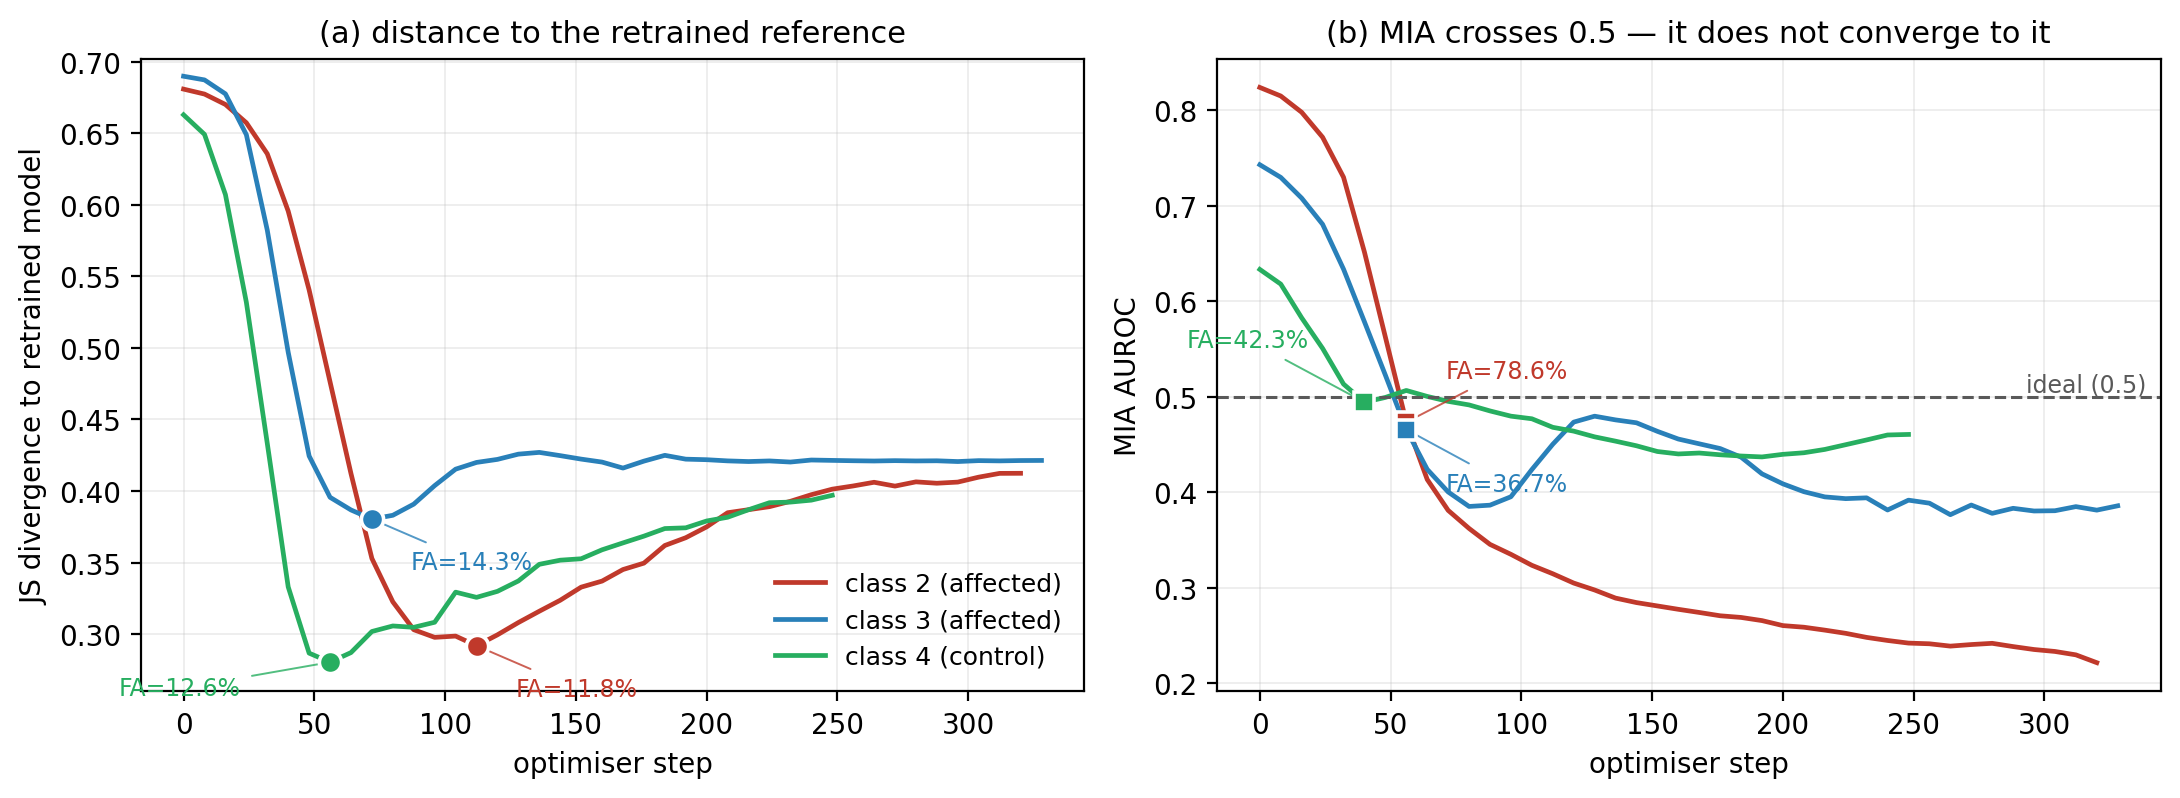
\includegraphics[width=\textwidth]{fig_trajectory.png}
\caption{\textbf{Unlearning overshoots the model it is trying to imitate, and
MIA cannot detect it.} \textbf{(a)}~Jensen--Shannon divergence to a
retrained-from-scratch reference along the unlearning trajectory. The curve is
U-shaped: the model first moves toward the reference, attains a minimum, then
moves away. Markers give the minimum, annotated with the forget accuracy there
($11.8$--$14.3\%$)---\emph{above} the $11.1\%$ chance level, whereas dual
stopping halts at ${\approx}7\%$. \textbf{(b)}~MIA AUROC on the same axis. It
sweeps \emph{through} the ideal $0.5$ rather than converging to it, so
$|\mathrm{MIA}-0.5|$ is minimised at the crossing. On class~2 that crossing
occurs while the model still classifies $78.6\%$ of the forget set
correctly.}
\label{fig:trajectory}
\end{figure}

\paragraph{The minimum is interior, and the current rule is past it.}
Divergence to the reference falls from $0.66$--$0.69$ at initialisation to
$0.28$--$0.38$, then rises again to $0.40$--$0.42$. So unlearning genuinely
moves the model toward a retrained one before moving away: over-forgetting is
not a metric artefact but a real overshoot in function space. The minimum lies
at $\mathrm{FA} = 11.8\%$, $14.3\%$ and $12.6\%$ for the three classes, while
dual stopping halts at ${\approx}7\%$ (\S\ref{sec:overforget}) --- past the
optimum in every case. Stopping at the minimum instead is close to free: test
accuracy changes by $-0.06$, $-0.03$ and $+0.79$pp and retain accuracy by
$+0.06$, $+0.36$ and $+0.08$pp. On the same trajectory it reduces divergence by
$0.016$, $0.003$ and $0.007$, and reduces $|\mathrm{MIA}-0.5|$ by $0.017$ and
$0.015$ on the two affected classes while moving the control by $+0.006$. This
is the pattern the criterion of \S\ref{sec:overforget} failed to produce:
the affected classes improve and the control stays put.

\paragraph{But the optimum is shallow, so we do not propose a numeric target.}
The three minima fall within $2.5$pp of one another in forget accuracy, which
invites the conclusion that ``stop at $\mathrm{FA}\approx 13\%$'' is a
deployable rule. The basin does not support that reading. Taking every
checkpoint within $5\%$ of the minimum divergence, the corresponding forget
accuracy spans $10.2$--$26.3\%$, $3.5$--$36.7\%$ and $6.9$--$21.9\%$ on the
three classes---$3.5$--$36.7\%$ overall. The agreement between the three
\emph{argmin} values is therefore largely a coincidence of where the snapshots
happened to land, and a single tuned number would not transfer. What the data
does support is directional and, we think, more useful: the optimum sits
\emph{above} the chance level, and a rule that drives forget accuracy to or
below chance is on the wrong side of it.

\paragraph{$|\mathrm{MIA}-0.5|$ is not an optimisation target.}
Panel~(b) is the more consequential finding. MIA AUROC does not converge to
$0.5$; it \emph{passes through} it, falling from $0.82$, $0.74$ and $0.63$ at
initialisation to $0.22$, $0.39$ and $0.46$ at the end. Consequently
$|\mathrm{MIA}-0.5|$ is minimised wherever the trajectory happens to cross,
which carries no information about unlearning quality. On class~2 the crossing
occurs at $\mathrm{FA} = 78.6\%$: a model that has barely forgotten anything
attains a \emph{perfect} MIA score. The two criteria also disagree about where
to stop, and in opposite directions---the divergence minimum and the MIA
minimum are $56$ steps apart on class~2, $56$ steps apart the other way on
class~3, and $8$ steps apart on class~4.

This sharpens the observation of \S\ref{sec:experiments} that a pre-unlearning
model already scores MIA $=0.533$. That was a single point; here we see the
whole path, and it shows that MIA $\approx 0.5$ is attainable at almost any
stage of unlearning, including stages with no meaningful forgetting at all.
Reporting MIA alongside forget accuracy is therefore not merely advisable but
necessary, and \emph{optimising} $|\mathrm{MIA}-0.5|$---which a practitioner
reading ``ideal $=0.5$'' might reasonably attempt---selects an arbitrary point
on the trajectory.

\paragraph{What remains unresolved.}
Stopping at the divergence minimum reduces over-forgetting without eliminating
it: class~2 still attains MIA $=0.315$ there, far from $0.5$. Nor do we have a
deployable rule, since locating the minimum requires the retrained reference
that unlearning exists to avoid, and the basin is too flat for a fixed forget
accuracy to stand in for it. We report the diagnosis---the stopping rule halts
on the wrong side of a real optimum---and leave a practical criterion open.
Whether the effect holds beyond the three PathMNIST classes measured here is
also untested; the experiment costs one unlearning run plus one retrained
reference per class.

% ============================================================
\section{Limitations in Full}\label{app:limitations}

\paragraph{Compute scales with classes and with data scarcity, and we cannot
predict it.} At \rev{its 15-epoch cap} \ours{} leaves STL-10 at
FA~$=75.7\%$, and an earlier version of this paper reported that as a failure
mode of the hard constraint on small forget sets. That diagnosis was wrong in
its conclusion though right about its cause. With 500 training images per class
the forget set yields only 4 mini-batches per epoch, ${\sim}60$ update steps in
total, and every step conflicts with the retain gradient---so progress per step
is small and the budget expires before forgetting completes. At 60 epochs, over
the same three seeds \rev{and with a per-step check and a $1\%$ target}, FA falls
to $1.73 \pm \rev{0.95}\%$ with RA~$=98.87\%$ \rev{(with the default $10\%$
target a single 60-epoch run stops at $9.2\%$)}. CIFAR-100
behaves the same way for a different reason: its per-class forget sets are small
because there are a hundred of them, and at 60 epochs its nine-class mean falls
from $4.07\%$ to $1.27 \pm \rev{0.39}\%$, bringing the $1\%$ chance level inside one
standard deviation. Neither constraint was infeasible; both runs were truncated.

What survives as a limitation is that we cannot say in advance how much budget a
new dataset needs. The binding resource is optimiser steps rather than epochs or
examples, and \ours{} offers no way to predict the requirement beyond monitoring
forget accuracy and continuing until the tolerance is met. A practitioner
deploying on an unfamiliar dataset should expect to discover the budget
empirically, and should treat a shared epoch count copied from another dataset
as a likely under-estimate.


\paragraph{Sample-level forgetting works, but at a cost the method cannot
control.} Every result in this paper removes a whole class. We tested the other
standard request type---forgetting a random subset of training points---on
CIFAR-10 at $1\%$ and $5\%$ of the training set, and report it as a scope limit
rather than a capability.

Two things go wrong, and they are different in kind. First, the forget objective
degenerates. \klr{} draws its power from the forget class being \emph{absent}
from the retain set, which drives $p_r$'s mass on that class to ${\sim}0$
(measured: $0.0002$); when the forget set is a random subset, the retain set
still covers every class and $p_r$ is uniform to three decimals
($0.100,0.100,\dots$). \klr{} therefore reduces exactly to
\texttt{kl\_uniform} in this regime, and the target carries no information about
\emph{which} points to forget. Second, dual stopping does not fire: the retain
budget is multiplicative on an initial retain loss of $0.0018$, so even at
$\alpha = 100$ both stopping-armed runs halted on the budget with forget accuracy
still at ${\sim}99.5\%$. A multiplicative budget is the wrong instrument against
a converged model; an absolute floor would be the right one.

Given a fixed 60-epoch budget and no stopping, forgetting does occur---forget
accuracy falls to $58.4\%$ at $1\%$ and $71.8\%$ at $5\%$---but
indiscriminately: retain accuracy falls from ${\sim}100\%$ to $73.2\%$ and test
accuracy to $71.9\%$, and forget accuracy ends \emph{below} test accuracy, which
is over-forgetting by the standard for this setting (a correctly unlearned point
should look like an unseen point of the same class, i.e.\ $\mathrm{FA}\approx
\mathrm{TA}$). The method has no mechanism to stop at that crossing.

The one clearly positive finding is the ablation. Removing the projection at
equal budget collapses the model completely: retain accuracy $14.2\%$ versus
$73.2\%$ with it, and test accuracy $17.1\%$ versus $71.9\%$---a $59$pp and
$55$pp difference respectively, far larger than the projection's effect in the
class-level ablation of Table~\ref{tab:ablation}. When forget and retain
gradients are drawn from the same distribution the conflict is near-total (the
projection fires on $100\%$ of steps), and the retain constraint is the only
thing keeping the model intact. The guarantee is therefore \emph{more}
load-bearing here, not less---which is why we regard sample-level forgetting as
a direction the constraint supports and the objective does not yet.

\paragraph{Mini-batch scope of the guarantee.} Theorem~\ref{thm:retain_safety}
bounds the \emph{sampled} retain objective---the quantity \ours{} projects
against---not the full-population retain loss. A population-exact per-step
guarantee would require controlling the gradient-variance term and is future
work.

\paragraph{The comparison with the closest prior work is structural, not
empirical.} Our separation from soft conflict-resolution methods
\citep{patel2025learning} rests on Theorem~\ref{thm:separation}(iv) and
Table~\ref{tab:properties}, both of which argue from the definition of the
update rule. We have not reimplemented that method and run it on our stack, so
we make no claim about how the two compare on accuracy, forgetting, or MIA. A
like-for-like empirical comparison is the most important piece of missing
evidence in this paper. Two related experiments are reported and should not be
mistaken for it: the projection-only ablation, isolating the projection from
\ours{}'s other three components (Table~\ref{tab:cifar10}), and the
projection-strength sweep, which interpolates our own update between a soft
penalty and the hard constraint (\S\ref{sec:strength}). Both test the mechanism;
neither runs the cited method.

\paragraph{Floating-point exactness.} The guarantee holds to float32 precision
(\S\ref{sec:alignment}); exact arithmetic would require float64 inner products.

\added{\paragraph{BatchNorm robustness is bought with compute, and is scoped.}
BN-robust \ours{} (\S\ref{sec:bn_robust}) survives the recalibration attack at
about seven times the wall-clock of the default configuration, because forgetting
that has to happen in the weights takes more steps. It was evaluated on two
datasets, CIFAR-10 (every class) and MNIST, and on base models that differ from
those behind the rest of the paper. It also defends only the normalisation
statistics: an attacker who modifies weights, as in the fine-tuning recovery
below, is outside what it changes.}

\paragraph{\rev{Sequential unlearning and fine-tuning recovery.}}
\rev{\emph{Sequential unlearning}: forgetting classes $0$, then $1$, then $2$
from each resulting checkpoint takes test accuracy $86.1 \to 76.8 \to 69.1$ and
retain accuracy $100.0 \to 89.7 \to 80.7$, with forget accuracy on the newest
class at most $2.7\%$. The decline is what forgetting does to these metrics,
not damage. TA counts every forgotten class's test images as errors, so fully
forgotten classes alone take it to $0.9$, $0.8$ and $0.7$ times the
retained-class accuracy (with the base model's $95.5\%$: $86.0$, $76.4$ and
$66.9\%$); RA is measured on a retain set that still contains the
earlier-forgotten classes, so fully forgotten classes take it to at most $8/9$
and $7/9$ ($88.9\%$ and $77.8\%$). The observed values sit at or above these
levels, so the retained classes are not damaged cumulatively. They sit above
them because earlier-forgotten classes partly return: an RA of $80.7\%$ requires
the two earlier classes to average at least $13\%$ training accuracy, above the
$10\%$ chance level. A sequential deployment should therefore re-check every
forgotten class after each request.} \emph{Fine-tuning recovery}: retraining the unlearned model on
$50$ forget-class samples raises forget accuracy from $1.9\%$ to $7.1\%$ after
five epochs and $51.3\%$ after ten---though by then the model is no longer
usable ($\mathrm{TA} = 34.6\%$, $\mathrm{RA} = 47.9\%$), so the attack recovers
the class only by destroying the model it attacks. \ours{} also does not provide
formal $(\varepsilon,\delta)$-DP guarantees.

\section{Per-Class Results}\label{app:perclass}

The main text reports per-dataset aggregates (Table~\ref{tab:cross}). Because a
mean over classes can conceal a method that succeeds on easy classes and fails on
hard ones, we report every class individually. Each row is the mean $\pm$
standard deviation over seeds $\{42,123,456\}$. CIFAR-100 per-class results
appear in the main text (Table~\ref{tab:cifar100}); the raw per-run CSVs for all
75 runs are released with the code.

\begin{figure}[t]
\centering
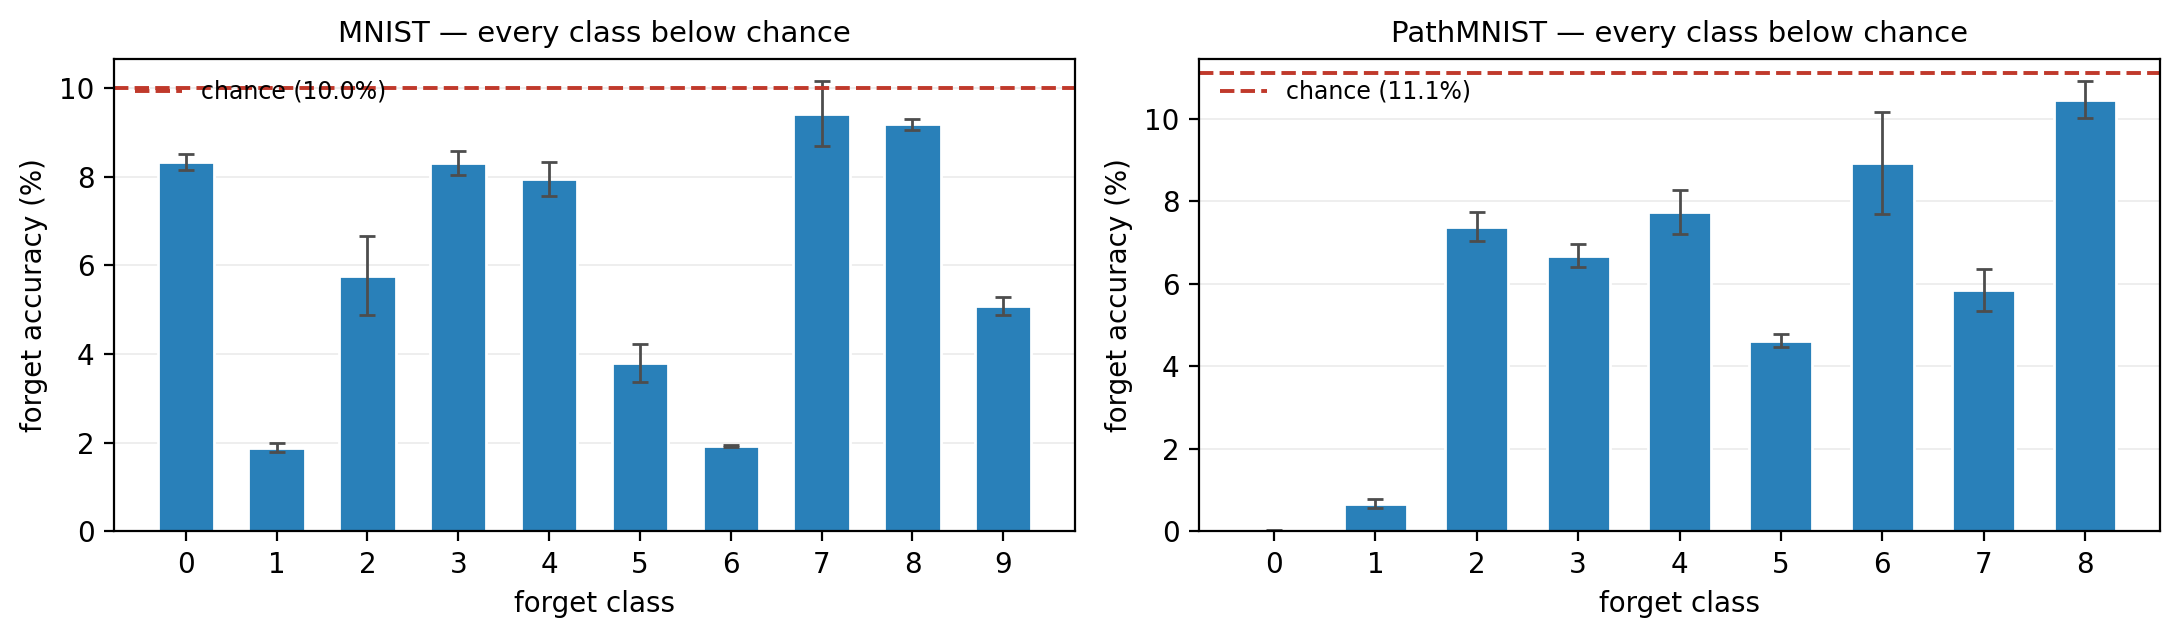
\includegraphics[width=\textwidth]{fig_perclass.png}
\caption{\textbf{Per-class forget accuracy} (mean $\pm$ std over three seeds).
Every MNIST and PathMNIST class individually falls below its chance level, so
the per-dataset means of Table~\ref{tab:cross} are not concealing a class that
fails.}
\label{fig:perclass}
\end{figure}

\subsection{MNIST (all 10 classes)}

Table~\ref{tab:app_mnist} gives all ten MNIST classes. Every class individually
falls below the $10\%$ chance level, with per-class mean FA ranging from
$1.89\%$ (class~1) to $9.42\%$ (class~7); the aggregate is therefore not
concealing a failure. Retain accuracy is essentially constant across classes
($99.42$--$99.54\%$), and MIA stays within $0.017$ of the ideal $0.5$ for every
class. Seed variance is small throughout (the largest FA standard deviation
across classes is $0.89$pp), indicating the procedure is stable rather than
seed-lucky.

\begin{table}[t]
\centering
\caption{\textbf{MNIST per-class forgetting} (mean $\pm$ std over 3 seeds).
Chance level is $10.0\%$; every class attains FA below it. TA is measured on the
full test set, so it necessarily drops by ${\sim}10$pp relative to the
$99\%$ base model once the forget class is correctly no longer recognised.}
\label{tab:app_mnist}
\begin{tabular}{@{}ccccc@{}}
\toprule
Forget class & TA (\%) & FA (\%)$\downarrow$ & RA (\%) & MIA \\
\midrule
0 & $90.26 \pm 0.05$ & $8.33 \pm 0.18$ & $99.42 \pm 0.00$ & $0.495 \pm 0.002$ \\
1 & $88.29 \pm 0.01$ & $1.89 \pm 0.09$ & $99.50 \pm 0.02$ & $0.512 \pm 0.001$ \\
2 & $89.68 \pm 0.07$ & $5.77 \pm 0.89$ & $99.51 \pm 0.01$ & $0.491 \pm 0.001$ \\
3 & $90.37 \pm 0.02$ & $8.31 \pm 0.27$ & $99.45 \pm 0.01$ & $0.483 \pm 0.001$ \\
4 & $90.22 \pm 0.01$ & $7.95 \pm 0.39$ & $99.43 \pm 0.02$ & $0.510 \pm 0.001$ \\
5 & $90.76 \pm 0.04$ & $3.80 \pm 0.43$ & $99.52 \pm 0.03$ & $0.499 \pm 0.001$ \\
6 & $90.08 \pm 0.02$ & $1.92 \pm 0.03$ & $99.50 \pm 0.02$ & $0.501 \pm 0.001$ \\
7 & $90.03 \pm 0.03$ & $9.42 \pm 0.74$ & $99.51 \pm 0.01$ & $0.490 \pm 0.000$ \\
8 & $90.36 \pm 0.03$ & $9.19 \pm 0.13$ & $99.50 \pm 0.02$ & $0.486 \pm 0.001$ \\
9 & $89.97 \pm 0.05$ & $5.09 \pm 0.21$ & $99.54 \pm 0.02$ & $0.503 \pm 0.000$ \\
\midrule
\textbf{Mean} & $\mathbf{90.00}$ & $\mathbf{6.17}$ & $\mathbf{99.49}$ & $\mathbf{0.497}$ \\
\bottomrule
\end{tabular}
\end{table}

\subsection{PathMNIST (all 9 classes)}

Table~\ref{tab:app_pathmnist} gives all nine PathMNIST tissue classes. Every
class again falls below the $11.1\%$ chance level, from $0.02\%$ (class~0) to
$10.46\%$ (class~8). Two observations deserve stating explicitly rather than
being averaged away.

First, the spread is far wider than on MNIST---per-class TA ranges from
$73.23\%$ to $89.28\%$---reflecting genuinely unequal class difficulty in
histopathology rather than instability: within-class seed variance remains small
(largest FA standard deviation $1.23$pp).

Second, and more importantly, \textbf{MIA AUROC is not uniformly near $0.5$}:
class~2 reaches $0.298$ and class~3 $0.388$, both well \emph{below} the ideal.
A value substantially below $0.5$ indicates that forget-class training samples
have become \emph{harder} to classify than forget-class test samples---the
signature of \emph{over}-forgetting, in which the unlearned model is
distinguishable from a retrained one in the opposite direction to a privacy
leak. It is detectable precisely because we report MIA per class and treat
distance from $0.5$ in either direction as a defect. We flag this as a real
limitation of the current stopping rule on PathMNIST: dual stopping targets FA,
which does not constrain how far past the retrained model's output statistics the
optimiser travels.

\begin{table}[t]
\centering
\caption{\textbf{PathMNIST per-class forgetting} (mean $\pm$ std over 3 seeds).
Chance level is $11.1\%$; every class attains FA below it. $^{\dagger}$Classes~2
and~3 show MIA well below the ideal $0.5$, indicating over-forgetting (see
text).}
\label{tab:app_pathmnist}
\begin{tabular}{@{}ccccc@{}}
\toprule
Forget class & TA (\%) & FA (\%)$\downarrow$ & RA (\%) & MIA \\
\midrule
0 & $73.23 \pm 0.06$ & $0.02 \pm 0.02$ & $99.01 \pm 0.01$ & $0.511 \pm 0.003$ \\
1 & $78.66 \pm 0.26$ & $0.68 \pm 0.12$ & $98.48 \pm 0.08$ & $0.473 \pm 0.003$ \\
2$^{\dagger}$ & $89.28 \pm 0.12$ & $7.38 \pm 0.35$ & $99.02 \pm 0.02$ & $0.298 \pm 0.003$ \\
3$^{\dagger}$ & $82.40 \pm 0.12$ & $6.68 \pm 0.28$ & $98.86 \pm 0.02$ & $0.388 \pm 0.005$ \\
4 & $78.04 \pm 0.08$ & $7.73 \pm 0.53$ & $98.95 \pm 0.03$ & $0.502 \pm 0.001$ \\
5 & $84.58 \pm 0.03$ & $4.62 \pm 0.15$ & $98.32 \pm 0.02$ & $0.548 \pm 0.001$ \\
6 & $78.58 \pm 0.25$ & $8.93 \pm 1.23$ & $98.77 \pm 0.06$ & $0.541 \pm 0.001$ \\
7 & $88.48 \pm 0.14$ & $5.85 \pm 0.50$ & $99.25 \pm 0.01$ & $0.562 \pm 0.001$ \\
8 & $75.36 \pm 0.04$ & $10.46 \pm 0.45$ & $99.28 \pm 0.03$ & $0.525 \pm 0.001$ \\
\midrule
\textbf{Mean} & $\mathbf{80.96}$ & $\mathbf{5.82}$ & $\mathbf{98.88}$ & $\mathbf{0.483}$ \\
\bottomrule
\end{tabular}
\end{table}

\paragraph{On the per-dataset MIA aggregate.}
The PathMNIST aggregate of $0.483 \pm 0.084$ in Table~\ref{tab:cross} is within
$0.017$ of ideal, but its standard deviation is an order of magnitude larger
than any other dataset's precisely because of classes~2 and~3. The aggregate is
accurate but uninformative here; this is a concrete instance of the more general
point of \S\ref{sec:experiments} that MIA must be read alongside FA, and
per-class rather than only in aggregate.

\begingroup\color{revised}% ---- new appendix subsection: added up to \endgroup
\subsection{BN-robust \ours{} on all ten CIFAR-10 classes}\label{app:bnrobust_perclass}

Table~\ref{tab:app_bnrobust} gives every CIFAR-10 class under the recalibration
attack of \S\ref{sec:bn_robust}, one seed per class (class~0 has three seeds in
Table~\ref{tab:bnrobust}). ``Pre'' and ``post'' are FA under test-time transforms
before and after \texttt{update\_bn} on the retain set. All runs share the
$93.97\%$ base of \S\ref{sec:bn_robust}. The calibrated runs here read the
stopping FA on the full retain set rather than the $10{,}240$-image subset; on
class~0 the two made identical stopping decisions (\S\ref{sec:bn_robust}).

\begin{table}[t]
\centering\color{revised}
\caption{\added{\textbf{BN-robust \ours{} per class} (CIFAR-10, seed~$42$). The
frozen-statistics configuration is recovered on every class. BN-robust is not,
under either stopping rule, and with calibrated stopping every class ships within
three standard errors of chance ($11.3\%$). Epochs ``$25{\to}22$'': the run
reached the cap and its best epoch was shipped.}}
\label{tab:app_bnrobust}
\small
\setlength{\tabcolsep}{4pt}
\begin{tabular}{@{}cccccccccc@{}}
\toprule
& \multicolumn{2}{c}{Frozen} & \multicolumn{2}{c}{BN-robust, naive}
& \multicolumn{5}{c}{BN-robust, calibrated} \\
\cmidrule(lr){2-3}\cmidrule(lr){4-5}\cmidrule(l){6-10}
Class & pre & post & pre & post & pre & post & epochs & TA & RA \\
\midrule
0 & $8.76$ & $99.22$ & $9.24$ & $9.28$ & $9.22$ & $9.24$ & 13 & $84.35$ & $95.60$ \\
1 & $2.40$ & $97.60$ & $10.66$ & $10.66$ & $6.66$ & $6.66$ & 8 & $84.56$ & $96.19$ \\
2 & $6.52$ & $98.30$ & $11.18$ & $11.16$ & $9.90$ & $9.92$ & 15 & $85.07$ & $95.27$ \\
3 & $4.78$ & $94.82$ & $11.30$ & $11.30$ & $10.00$ & $9.98$ & 16 & $85.92$ & $96.26$ \\
4 & $4.84$ & $97.34$ & $13.32$ & $13.34$ & $10.18$ & $10.16$ & $25{\to}22$ & $84.88$ & $94.74$ \\
5 & $7.28$ & $94.70$ & $8.78$ & $8.78$ & $9.40$ & $9.42$ & 12 & $84.52$ & $94.64$ \\
6 & $9.18$ & $99.14$ & $7.20$ & $7.20$ & $7.30$ & $7.30$ & 8 & $83.32$ & $94.41$ \\
7 & $3.38$ & $96.20$ & $11.36$ & $11.34$ & $9.12$ & $9.12$ & 10 & $84.49$ & $95.24$ \\
8 & $4.54$ & $99.26$ & $16.74$ & $16.68$ & $9.74$ & $9.68$ & 14 & $83.59$ & $94.67$ \\
9 & $2.52$ & $98.16$ & $15.44$ & $15.42$ & $8.92$ & $8.92$ & 11 & $83.84$ & $95.01$ \\
\midrule
Mean & $5.42$ & $97.47$ & $11.52$ & $11.52$ & $9.04$ & $9.04$ & --- & $84.45$ & $95.20$ \\
\bottomrule
\end{tabular}
\end{table}

\begin{figure}[t]
\centering\color{revised}
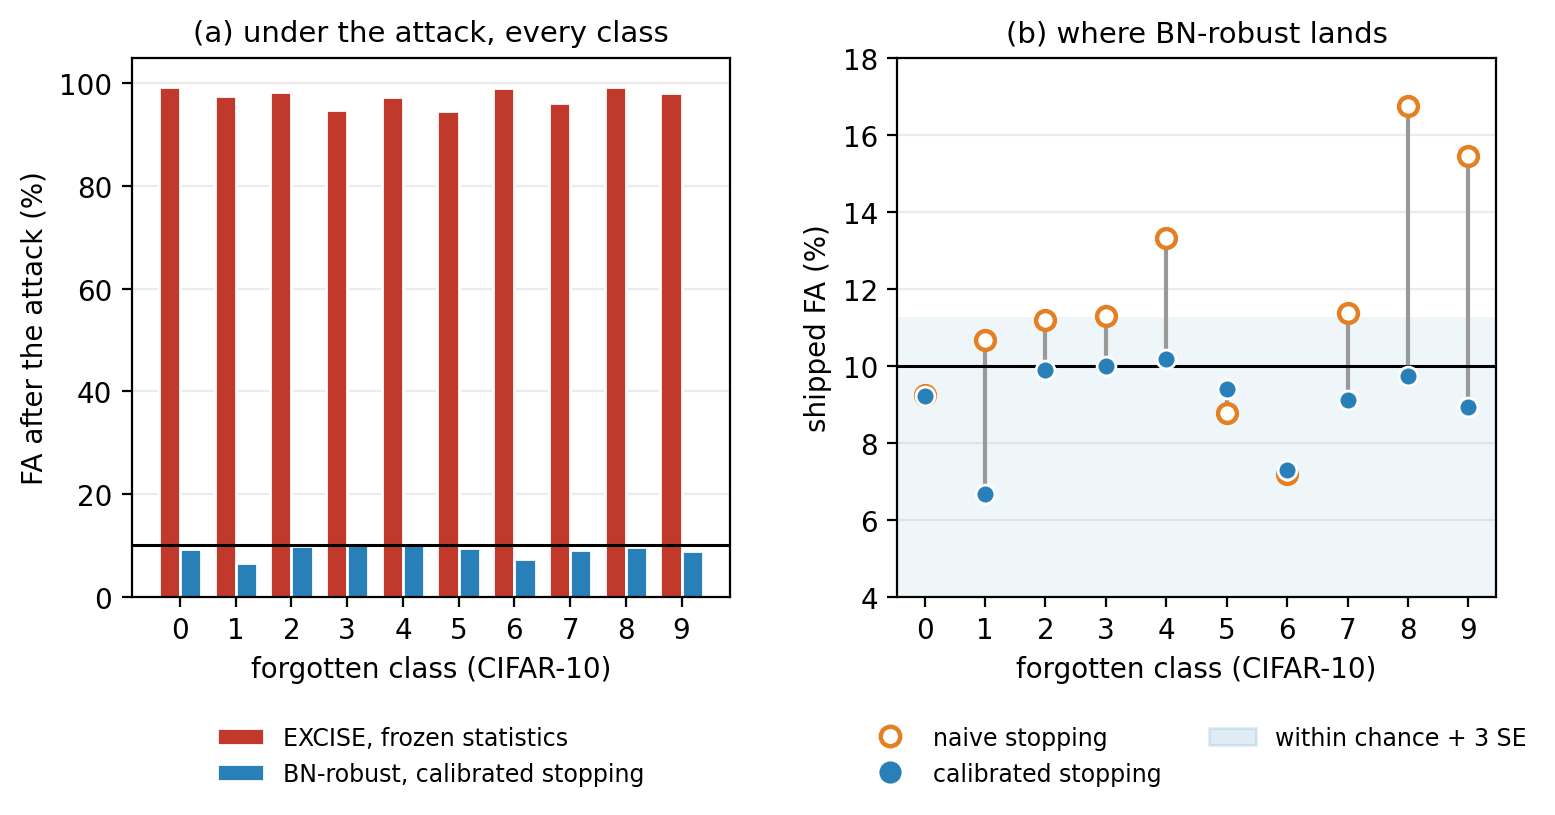
\includegraphics[width=\textwidth]{fig_bnrobust_perclass.png}
\caption{\added{\textbf{BN-robust on all ten CIFAR-10 classes} (seed~$42$; the data of
Table~\ref{tab:app_bnrobust}). (a)~Under the attack, the frozen-statistics
configuration is recovered on every class and BN-robust on none. (b)~Where
BN-robust ships: with naive stopping (open) five classes land above chance
$+\,3$\,SE; with calibrated stopping (filled), none do.}}
\label{fig:app_bnrobust}
\end{figure}
\endgroup% ---- end of the added appendix subsection

% ------------------------------------------------------------
\section{Hyperparameter Configuration}\label{app:hyper}

Table~\ref{tab:app_shared} lists the settings shared across all datasets and
Table~\ref{tab:app_perdataset} the per-dataset settings. All are released as YAML
configuration files; the reported runs use them unmodified.

\begin{table}[t]
\centering
\caption{\textbf{Shared hyperparameters} (identical for all six datasets). The
two components removed from \ours{} are listed explicitly with value $0$, since
they remain available as flags for the ablation of \S\ref{sec:ablation}.}
\label{tab:app_shared}
\begin{tabular}{@{}llll@{}}
\toprule
Symbol & Flag & Value & Role \\
\midrule
$\mu$ & \texttt{--momentum} & $0.9$ & momentum; projection applied \emph{after} accumulation \\
$c$ & \texttt{--max\_grad\_norm} & $1.0$ & clip on $d_t$, \emph{before} accumulation \\
$\lambda_{\mathrm{wd}}$ & \texttt{--weight\_decay} & $5\times10^{-4}$ & weight decay, applied inside $d_t$ \\
$T_{\mathrm{KD}}$ & \texttt{--temperature} & $4.0$ & distillation temperature \\
--- & \texttt{--forget\_objective} & \klr{} & KL toward retain-confusion $p_r$ \\
--- & \texttt{--batch\_size} & $128$ & forget and retain mini-batch size \\
--- & \texttt{--fa\_check\_freq} & $50$ & intra-epoch FA check interval (batches) \\
--- & \texttt{--seed} & $\{42,123,456\}$ & three seeds per task \\
\midrule
\multicolumn{4}{@{}l}{\emph{Removed components (retained as ablation flags only)}} \\
$\lambda$ & \texttt{--rep\_weight} & $0.0$ & representation erasure (removed) \\
$\gamma$ & \texttt{--forget\_gate} & $0.0$ & entropy gate (removed) \\
\bottomrule
\end{tabular}
\end{table}

\begin{table}[t]
\centering
\caption{\textbf{Per-dataset hyperparameters.} $K$ is the number of classes.
Note that the forget-accuracy target $\tau_F$ is set to the chance level
$100/K$ for every dataset---it is not tuned per dataset, but derived from the
task.}
\label{tab:app_perdataset}
\begin{tabular}{@{}lcccccc@{}}
\toprule
Dataset & $K$ & Epochs $T$ & $\eta$ & $\beta$ (KD) & $\alpha$ (retain budget) & $\tau_F = 100/K$ \\
\midrule
CIFAR-10  & 10  & 15 & $5\times10^{-4}$ & $2.0$ & $5.0$ & $10.0\%$ \\
CIFAR-100 & 100 & 20 & $5\times10^{-4}$ & $2.0$ & $5.0$ & $\phantom{0}1.0\%$ \\
MNIST     & 10  & 12 & $2\times10^{-4}$ & $3.0$ & $4.0$ & $10.0\%$ \\
SVHN      & 10  & 15 & $2\times10^{-4}$ & $3.0$ & $5.0$ & $10.0\%$ \\
STL-10    & 10  & 15 & $2\times10^{-4}$ & $5.0$ & $5.0$ & $10.0\%$ \\
PathMNIST & \phantom{0}9 & 12 & $2\times10^{-4}$ & $5.0$ & $4.0$ & $11.1\%$ \\
\bottomrule
\end{tabular}
\end{table}

\paragraph{Tuning effort.}
Only four quantities vary across datasets: the epoch cap $T$, the learning rate
$\eta$, the KD weight $\beta$, and the retain budget $\alpha$. The learning rate
takes one of two values ($5\times10^{-4}$ for the CIFAR datasets,
$2\times10^{-4}$ elsewhere), $\beta$ one of three, and $\alpha$ one of two. The
forget target $\tau_F$ is not tuned at all: it is fixed to the chance level
$100/K$ implied by the task. Notably, $\mu$, $c$, $\lambda_{\mathrm{wd}}$, and
$T_{\mathrm{KD}}$---the four quantities that enter the guarantee of
Theorem~\ref{thm:app_main}---are held constant across all six datasets, so the
bound $\tfrac12 L\eta^2(c/(1-\mu))^2$ varies across datasets only through
$\eta$ (and through the dataset-dependent smoothness constant $L$).

\paragraph{A note on defaults.}
The command-line default for \texttt{--max\_grad\_norm} in the released code is
$5.0$, whereas every configuration file sets $c=1.0$. Runs launched without
\texttt{--config} would therefore use a different clip threshold, and a
correspondingly weaker constant in
(\ref{eq:app_c}). All results in this paper use the configuration files. We note
this because the value of $c$ enters the guarantee directly, so it should not be
inherited silently from a default.

% ------------------------------------------------------------
\section{Distance to the Retrained Model: A Refuted Hypothesis}\label{app:d2r}

This appendix reports a negative result. We formed a hypothesis about why
\ours{} over-forgets on two PathMNIST classes, derived a deployable fix from it,
pre-committed to a falsifiable prediction, ran the experiment, and the
prediction did not hold. We report it in full because the experiment also
produced the diagnosis that we believe is correct, and because the refuted
hypothesis concerns \ours{}'s own forget objective.

\subsection{The defect, and the hypothesis}

Per-class reporting (Appendix~\ref{app:perclass}) showed that on PathMNIST
classes~2 and~3, MIA AUROC reaches $0.298$ and $0.388$---far \emph{below} the
ideal $0.5$. Forget accuracy is satisfied on both, so FA alone certifies these
runs as successes when they are not. A value below $0.5$ means forget-class
training samples have become \emph{harder} to classify than forget-class test
samples: the model is still distinguishable from a retrained one, in the
opposite direction to a privacy leak.

\rev{An earlier version of our forget-side condition (Eq.~\ref{eq:problem}) was
$\KL(p_\theta(x_f)\,\|\,p_r) \le \epsilon$}, a statement about
\emph{distributions}, but dual stopping (\S\ref{sec:stopping}) implements
\rev{$\mathrm{FA} \le \tau_F$}, a statement about \emph{argmax}. These are not
equivalent, and we hypothesised that the discrepancy was the cause: FA cannot
distinguish (a)~$p_\theta(x_f)$ having moved \emph{to} the distribution a
retrained model produces from (b)~having moved \emph{past} it, since both give
$\mathrm{FA}\approx 0$.

The hypothesised fix was to enforce the constraint as stated. Since $p_r$ is
computed from the \emph{original} model, this needs no retrained reference and
is deployable: stop on $\KL(p_\theta(x_f)\|p_r)$ rather than on FA. We reasoned
that this quantity is minimised at $p_\theta = p_r$ and rises on either side, so
a stop-when-it-stops-improving rule would halt at the minimum---exactly the
point FA cannot locate.

\paragraph{Prediction (pre-committed).} Replacing FA stopping with KL stopping
would, on the affected classes, (1)~reduce $|\mathrm{MIA}-0.5|$, (2)~reduce
Jensen--Shannon divergence to a retrained reference, and (3)~not materially
worsen FA or RA, while leaving an unaffected control class approximately
unchanged.

\subsection{Design}

We retrained reference models without the forget class for PathMNIST classes~2
and~3 (affected) and class~4 (control, MIA already $0.501$), keeping all $K$
output heads so that output distributions remain comparable, and training all
three identically for a fixed 30-epoch cosine schedule so that no reference is
better converged than another. Arm~A is \ours{} with FA stopping (the deployed
configuration); arm~B disables FA stopping and enables KL stopping. Oracle
metrics are computed against the references: JS divergence between output
distributions on the forget set (primary), top-1 agreement with the reference,
Fr\'echet distance between penultimate features, and MIA.

The control class is the load-bearing part of the design: a criterion that
merely stops earlier everywhere would improve the affected classes while also
perturbing the control, whereas a targeted fix should leave the control alone.

\subsection{Result: the prediction fails}

Table~\ref{tab:app_klstop} reports the outcome. Across three classes and four
metrics, arm~B is better on 2 comparisons and worse on 10. The primary oracle
metric---JS divergence to the retrained model---is \emph{worse in all three
classes}. The control class degrades on every metric, which is precisely the
signature that rules out a targeted fix. Only class~3 improves on
$|\mathrm{MIA}-0.5|$.

\begin{table}[t]
\centering
\caption{\textbf{KL stopping vs.\ FA stopping on PathMNIST}, measured against
retrained references. Arrows mark the direction of improvement. The prediction
was that the affected classes would improve and the control would not move;
neither held.}
\label{tab:app_klstop}
\begin{tabular}{@{}llccccc@{}}
\toprule
Class & Arm & $|\mathrm{MIA}{-}0.5|\downarrow$ & JS$\downarrow$ &
agree \%$\uparrow$ & Fr\'echet$\downarrow$ & $\KL$ to $p_r$ \\
\midrule
\multirow{2}{*}{2 (affected)}
 & FA stop & $0.205$ & $0.308$ & $45.4$ & $185.7$ & $0.957$ \\
 & KL stop & $0.268$ & $0.412$ & $23.5$ & $332.0$ & $0.052$ \\
\midrule
\multirow{2}{*}{3 (affected)}
 & FA stop & $0.115$ & $0.382$ & $31.2$ & $375.2$ & $0.805$ \\
 & KL stop & $\mathbf{0.068}$ & $0.421$ & $\mathbf{39.8}$ & $780.1$ & $0.002$ \\
\midrule
\multirow{2}{*}{4 (control)}
 & FA stop & $0.001$ & $0.286$ & $38.7$ & $141.1$ & $1.510$ \\
 & KL stop & $0.044$ & $0.399$ & $12.3$ & $297.7$ & $0.116$ \\
\bottomrule
\end{tabular}
\end{table}

\paragraph{The proxy is anti-correlated with the oracle.}
A proxy is only usable if it tracks the quantity it stands in for. Across the
six checkpoints, the rank correlation between $\KL(p_\theta\|p_r)$ and JS
divergence to the retrained model is $\rho = -1.00$ (Pearson $-0.94$): the
ordering is perfectly inverted. Driving the deployable proxy toward zero moves
the model monotonically \emph{away} from the retrained reference. This is the
opposite of the relationship the hypothesis required.

\subsection{Why it failed}

\paragraph{(i) The criterion never fired.}
In all three runs of arm~B the terminating condition was the retain-loss budget,
not the KL rule. The reason is visible in the logged trajectories:
$\KL(p_\theta(x_f)\|p_r)$ decreases essentially monotonically (class~2:
$5.53 \to 0.05$ over 8 checks with zero increases; class~4: $2.73 \to 0.07$,
zero increases; class~3: $2.06 \to 0.002$ over 20 checks with 4 small
increases). It never turns back up, so a stop-when-it-stops-improving rule
cannot trigger. The U-shape the hypothesis assumed does not exist over the
range the optimiser traverses.

This is also a limitation of the test, and we state it plainly: because the KL
rule never fired and FA stopping was disabled, arm~B is in effect \ours{}
\emph{without forget-side stopping} (FA reaches $0.0$ in all three runs), which
is closer to the $-$Stopping ablation than to a KL-stopped method. The
comparison in Table~\ref{tab:app_klstop} is therefore evidence against the
criterion \emph{as specified}, not a clean contrast between two stopping rules.

\paragraph{(ii) $p_r$ is a global average; a retrained model routes per-sample.}
$p_r$ is a single distribution, the retain-set average softmax, and it is the
same target for every forget sample. A retrained model does something different:
it routes each forget-class image to whichever surviving class that particular
image most resembles, giving an input-dependent output distribution. Matching
$p_r$ more closely therefore makes the model's predictions on forget data
unnaturally homogeneous across samples. The agreement column is the evidence:
as $\KL$ to $p_r$ falls by one to three orders of magnitude, top-1 agreement
with the reference \emph{collapses} on two of the three classes
($45.4 \to 23.5$ on class~2, $38.7 \to 12.3$ on class~4). If $p_r$ were the
right target, matching it better should have raised agreement. Class~3 moves the
other way ($31.2 \to 39.8$), so the effect is not universal.

\paragraph{Confound we cannot separate.}
$\KL$ to $p_r$ decreases with training time while JS to the reference increases
over the observed range, so the two are mechanically anti-correlated and the
$\rho = -1.00$ figure partly reflects run duration rather than target quality
alone. The agreement collapse is the part of the evidence that speaks to the
target itself, and it rests on two of three classes. We therefore claim the
criterion is refuted, and treat the mechanism as well-supported but not
established.

\subsection{What the experiment did establish}

\paragraph{The FA rule overshoots its own target.}
All three FA-stopped runs halt at $\mathrm{FA} \approx 7\%$ against a target of
$11.1\%$ (the chance level), overshooting by $3.9$--$4.2$pp, because the
intra-epoch FA check is evaluated only every 50 batches. The over-forgetting we
set out to explain is thus at least partly a \emph{granularity} defect in how
the existing criterion is enforced, not evidence that FA is the wrong quantity.

\paragraph{Less unlearning was better on every class.}
JS divergence to the retrained model is lower at the earlier stopping point in
all three classes. Over the range we observe, the model is still moving toward
the retrained reference when FA stopping halts it, and continues away from it
afterwards. Combined with the overshoot above, this points to stopping
\emph{earlier and more precisely} rather than to replacing the stopped quantity.

\paragraph{Consequence for the method.}
We draw a narrower conclusion about \klr{} than the original formulation
implies. As a forget-side \emph{direction}, $p_r$ is a better target than the
uniform distribution (\S\ref{sec:forget_obj}). As a \emph{target to be minimised
to zero}, it is actively harmful. \rev{Accordingly Eq.~\ref{eq:problem} states
the forget condition on forget accuracy and uses the divergence only as the
direction of the search}, and we do not claim $p_r$ is what a retrained model produces on forget
inputs---the measurements here show it is not.

\subsection{Open question}

Where JS divergence to the retrained model is minimised along the unlearning
trajectory remains unmeasured. Since JS is still falling when FA stopping fires
and rising afterwards, a minimum exists between the base model and the FA-stopped
point; locating it would establish whether a single FA level identifies it across
classes, which would make it deployable, or whether it varies per class, which
would not.
This question is answered in \S\ref{sec:trajectory}: the minimum is interior, lies above the chance level, and the current rule stops past it.

% ------------------------------------------------------------
\section{Ethical and Societal Considerations}\label{app:ethics}

\paragraph{Unlearning as evidence removal.}
A method that makes a model indistinguishable from one retrained without
specific data could be misused to destroy evidence that problematic data was
used for training. This is a dual-use property of the unlearning goal itself
rather than of \ours{} specifically, but \ours{} does make it concrete. Partial
mitigation is that \ours{} leaves an audit trail by construction: projection-rate
logs, the FA trajectory, and retain-loss budget history are all recorded per run,
so an auditor with access to the logs can establish that unlearning was applied
and to what extent. We note this is mitigation, not prevention---an adversary who
controls the logs controls the audit.

\paragraph{Selective fairness degradation.}
Class-level unlearning removes all samples of a class, which may correspond to a
demographic group. Crucially, the accuracy degradation we observe is
\emph{not} confined to the forgotten class: test accuracy falls beyond what the
removed class alone accounts for, and the per-class spread on PathMNIST
(Appendix~\ref{app:perclass}) shows the effect is uneven across classes.
Deployers should therefore monitor per-class accuracy before and after
unlearning rather than only aggregate accuracy, which can conceal a
disproportionate cost borne by one group.

\paragraph{Over-forgetting as a distinct harm.}
The PathMNIST finding (Appendix~\ref{app:perclass}) shows that a model can be
pushed \emph{past} the retrained reference. This matters ethically as well as
technically: such a model is still distinguishable from one trained without the
data, so a deletion request has not been faithfully honoured, yet every
FA-based check reports success. Compliance evidence resting on forget accuracy
alone would be misleading here.

\paragraph{Regulatory gap.}
Approximate unlearning methods, including \ours{}, do not satisfy formal
$(\varepsilon,\delta)$-differential-privacy certification. Whether
MIA AUROC~$\approx 0.5$ constitutes legally sufficient ``erasure'' under
instruments such as the GDPR right to erasure remains an open legal question on
which we take no position. The per-step guarantee of
Theorem~\ref{thm:retain_safety} is a statement about \emph{retain-side utility},
not a privacy certificate, and should not be presented as one.

% ------------------------------------------------------------
\section{Reproducibility}\label{app:repro}

\paragraph{Artefacts.}
Code, YAML configuration files, per-run summary CSVs for all 75 runs, and the
BatchNorm-recalibration diagnostic are released in the anonymised repository.
\todo{Insert the anonymised repository URL.}
The archived $\mu=0$ results underlying Table~\ref{tab:momentum} are released
alongside the main results, so the momentum ablation can be re-derived without
re-running it.

\paragraph{Environment.}
PyTorch $\ge 2.0$ with CUDA; ResNet-18 (11.7M parameters) throughout. Runs were
executed on a single GPU. Datasets download automatically except PathMNIST,
which is obtained through \texttt{medmnist}.

\paragraph{Implementation details that affect results.}
\begin{itemize}
\item Momentum and weight decay are applied \emph{manually} so that the
projection acts on the post-momentum update; the underlying \texttt{torch} SGD
object is configured with \texttt{momentum=0}, \texttt{weight\_decay=0} and acts
only as a plain step. Reading the optimiser construction alone is therefore
misleading---see \S\ref{sec:optimiser} and Appendix~\ref{app:setup}.
\item Clipping is applied to $d_t$ before momentum accumulation, and \emph{not}
to the final update. Reversing this changes the effective step size by a factor
$1/(1-\mu)$ (Proposition~\ref{prop:clip}).
\item The projected update is rescaled to the pre-projection norm.
\item BatchNorm layers are set to \texttt{eval()} immediately after the model is
set to \texttt{train()}, so running statistics are frozen during unlearning.
\added{BN-robust \ours{} (\S\ref{sec:bn_robust}) instead recomputes them from
$512$ retain images before every step (\texttt{--bn\_robust exact
--bn\_recal\_samples 512}) and on the full retain set under test-time transforms
after the last step. It reads the stopping forget accuracy under statistics
recomputed from $10{,}240$ retain images (\texttt{--bn\_calibrated\_stop
--bn\_stop\_recal\_samples 10240}), ships the best epoch when the target is not
met (\texttt{--restore\_best\_epoch}), and uses an epoch cap of $25$.}
\item The retain-confusion distribution $p_r$ is precomputed once from the frozen
original model.
\item Forward hooks are registered on \texttt{layer3}, \texttt{layer4}, and
\texttt{avgpool} for feature-level diagnostics.
\item Configuration files set $c=1.0$; the CLI default is $5.0$ (see above).
\item All baselines are re-run within the same codebase under a unified MIA
protocol, rather than quoted from their source papers.
\end{itemize}

\paragraph{Determinism and seeds.}
Every 10-class task is run with seeds $\{42,123,456\}$ and reported as
mean~$\pm$~std; CIFAR-100 uses a single seed per class. Seed variance is small
(Appendix~\ref{app:perclass}). As an internal consistency check, the two
ablation variants that are no-ops under the shipped configuration
(\texttt{--rep\_weight 0}, \texttt{--forget\_gate 0}, both already $0$) produce
byte-identical metrics, confirming both that the runs are deterministic given a
seed and that those components are genuinely inactive.

\paragraph{Known reproduction caveats.}
The floating-point exactness of the guarantee is precision-dependent
(Remark~\ref{rem:float}): reference implementations should accumulate the
projection inner products in float64. Wall-clock timings depend on the GPU and
on how early dual stopping fires, so step counts rather than seconds are the
portable quantity.

\end{document}
"
\ifdefined\finalversion
  \definecolor{revised}{RGB}{0,0,0}
  \definecolor{revisedB}{RGB}{0,0,0}
\else
  \ifdefined\showpreviousround
    \definecolor{revised}{RGB}{204,85,0}
  \else
    \definecolor{revised}{RGB}{0,0,0}
  \fi
  \definecolor{revisedB}{RGB}{0,84,180}
\fi
\newcommand{\added}[1]{{\color{revised}#1}}
\newcommand{\rev}[1]{{\color{revisedB}#1}}

\newtheorem{theorem}{Theorem}
\newtheorem{proposition}{Proposition}
\newtheorem{lemma}{Lemma}
\newtheorem{corollary}{Corollary}
\theoremstyle{remark}
\newtheorem{remark}{Remark}
\theoremstyle{plain}

\title{Provably Retain-Safe Machine Unlearning\\ via Gradient Projection}

\author{\name Anonymous \email anonymous@example.com \\
        \addr Anonymous Institution}

\begin{document}
\maketitle
\suppressfloats[t]% Figure 1 goes to the top of page 2, not above the title

\begin{abstract}
Machine unlearning must remove a class's influence from a trained network
without damaging what the network should keep---a forget--retain trade-off dual
to the stability--plasticity trade-off of continual learning. We adapt A-GEM's
gradient projection so that every unlearning step lies in the retain-safe
half-space $\{u : \langle u,\gr\rangle \ge 0\}$, and apply it to the
post-momentum update the optimiser actually takes rather than to the raw
gradient. The resulting per-step retain-safety guarantee is exact for the
deployed optimiser; removing momentum to simplify the analysis instead
\rev{leaves forget accuracy far above chance on five of six datasets}. \ours{}
pairs the projected update with a
retain-confusion forget objective and stopping rules derived from explicit
tolerances. Across six datasets and 31 class-level forgetting tasks with
ResNet-18 it drives forget accuracy to \rev{within sampling error of} the chance
level on all six (two at a longer epoch budget), with retain accuracy at or above
$97.2\%$ on the 10-class datasets, and step-level logs \rev{of a CIFAR-10 run}
confirm the constraint at every step. \rev{On BatchNorm backbones, forgetting
learned against frozen normalisation statistics is undone by recomputing
them---as concurrent work finds for six of nine prior methods. A variant that
keeps the statistics consistent with the weights forgets to chance on every
CIFAR-10 class and on MNIST and survives that attack, including when the
attacker chooses the recalibration data.} We also find that the conventional
membership-inference
target of $0.5$ is the wrong reference point: a retrained model scores $0.69$ on
CIFAR-10, and between $0.31$ and $0.70$ across PathMNIST classes.
\end{abstract}

% ============================================================
\section{Introduction}\label{sec:intro}

Trained models increasingly need to demonstrably \emph{forget} specific
data---to honour deletion requests, revoke expired licences, or remove poisoned
samples. Retraining without the data does this exactly but is costly
(\rev{under an hour} for a ResNet-18 on CIFAR-10 on one A100, days for production
models), so \emph{machine unlearning} (MU) asks how to modify a trained model so
that it behaves as if the data had never been seen. The hard part is not erasing
the data's influence but doing so \emph{without collateral damage}: what must be
erased and what must be kept live in the same weights, so any step that degrades
the forgotten data also perturbs everything else.

\begin{figure}[t]
\centering\color{revisedB}
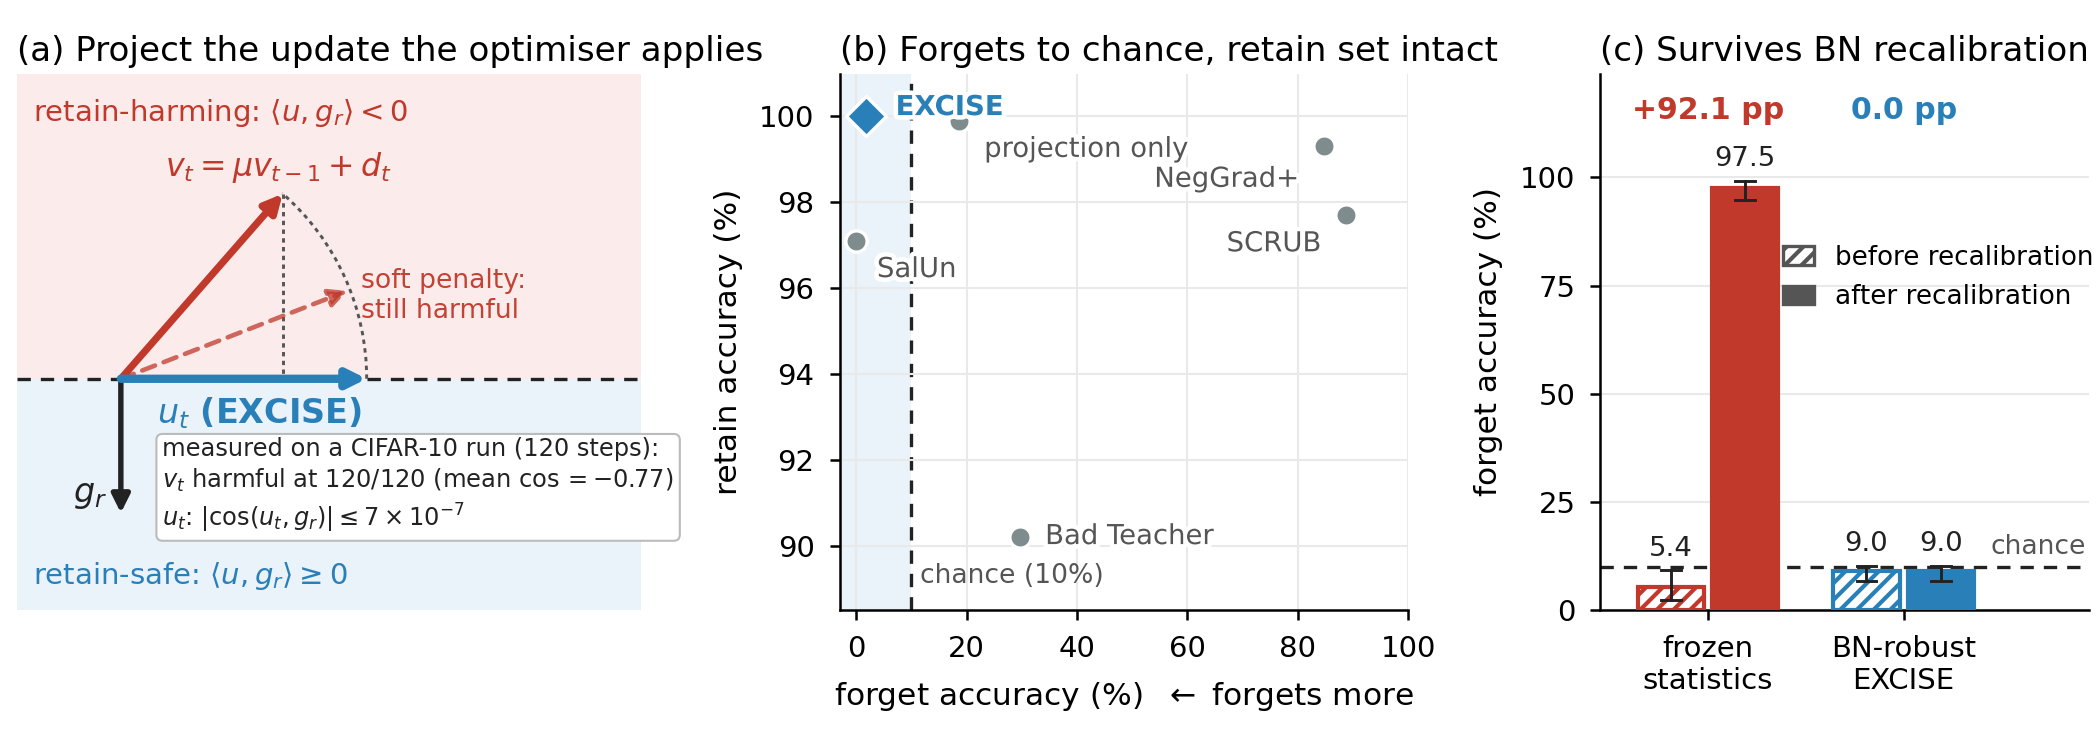
\includegraphics[width=\textwidth]{fig_teaser.png}
\caption{\rev{\textbf{\ours{} in one picture.} \textbf{(a)}~With momentum, the
update the optimiser applies is the accumulated $v_t$, and in unlearning it
points into the retain-harming half-space at every step. \ours{} projects $v_t$
onto the boundary and restores its length, so the applied $u_t$ cannot increase
the sampled retain loss to first order (Theorem~\ref{thm:retain_safety}); a
soft penalty only tilts the step, which stays harmful
(Theorem~\ref{thm:separation}). The boxed numbers are measured
(Figure~\ref{fig:guarantee}). \textbf{(b)}~On CIFAR-10 class~0, \ours{} is the
only method in Table~\ref{tab:cifar10} that forgets to chance with the retain
set intact. \textbf{(c)}~With frozen BatchNorm statistics, recomputing them on
retained data undoes the forgetting on every CIFAR-10 class; BN-robust \ours{}
does not move. Bars are means over the ten classes and whiskers their range
(Table~\ref{tab:app_bnrobust}).}}
\label{fig:teaser}
\end{figure}

\paragraph{The mirror image in continual learning.}
Continual learning (CL) faces the same problem with the sign reversed: learn a
new task while protecting old ones. \rev{One of its most direct answers} is not
a penalty but a \emph{constraint on the update}. A-GEM \citep{chaudhry2019agem} projects any
update $v$ with $\langle v, g_{\text{old}}\rangle < 0$ onto the half-space
$\{u : \langle u, g_{\text{old}}\rangle \ge 0\}$, so a step that would increase
old-task loss to first order is never taken. Unlearning lacks exactly this
guarantee: \rev{most} existing methods control retain damage with weighted
objectives, saliency masks or alternating updates (\S\ref{sec:related}), which
\rev{discourage retain-harming steps rather than exclude them}. We treat the retain set as CL's ``old task'' and
adopt the half-space constraint as the update rule for unlearning. The duality
has been noted before \citep{kurmanji2023unbounded,nguyen2020variational}, and
the forget--retain conflict has been targeted by a soft regulariser
\citep{patel2025learning}\added{ and by projecting updates away from a retain
gradient subspace \citep{hoang2024learn}}; what has not been done\rev{, to our
knowledge,} is to enforce the half-space constraint \rev{against the current
retain gradient}, at every step, on the vector the optimiser applies.

\paragraph{What it takes.}
Three design decisions \rev{complete the method}. \emph{Project the update, not
the gradient}: with momentum, the applied vector is the accumulated update, and
projecting the gradient certifies nothing about it
(Proposition~\ref{prop:counter}). Removing momentum would make the analysis
exact but \rev{leaves forget accuracy far above chance on five of six datasets}
(\S\ref{sec:momentum_ablation}), so we project the post-momentum update and make
the guarantee hold for the optimiser that runs. \emph{Push the forgotten class
toward the model's own retain-confusion distribution}, rather than the uniform
distribution no trained model produces\rev{; at equal test accuracy it forgets
further than gradient ascent and slightly further than a uniform target}
(\S\ref{sec:forget_obj}). \emph{Stop on explicit tolerances} for retain loss and
forget accuracy rather than on an epoch count (\S\ref{sec:stopping}).

\paragraph{Forgetting that survives the attack.}
A fourth issue came from the experiments. Forget batches contain a single
class and would corrupt BatchNorm running statistics, so the method freezes them
during unlearning---and the weights then learn to forget \emph{relative to}
statistics an attacker can replace: recomputing them on retained data restores
forget accuracy from ${\sim}1\%$ to ${\sim}100\%$ without changing a weight
(\S\ref{sec:bn_results}). \rev{The attack reaches beyond us. Concurrent work
\citep{kalani2026batchnorm} applies it to nine prior methods and recovers the
forgotten class for six of them; of the other three, gradient ascent forgets
only by destroying the model ($57\%$ retain accuracy), GA+FT does not forget
($68\%$ forget accuracy), and SCRUB keeps its forgetting at $88\%$ retain
accuracy. Whether a method survives depends less on the method than on how its
statistics are handled during unlearning: in \citet{kalani2026batchnorm},
mixing at least a quarter of retained data into SalUn's unlearning batches
removes its recovery, and our own reproductions of SalUn and Bad Teacher, which
end every epoch with a pass over retained data that recomputes the statistics,
are not recovered at all. BN-robust \ours{} makes survival a property of the
method rather than of how it is run: it keeps the statistics consistent with the
weights throughout unlearning, forgets to chance on every CIFAR-10 class and on
MNIST, survives the attack in every case we tried---including when the attacker
chooses the recalibration data---and keeps the per-step guarantee
(\S\ref{sec:bn_robust}). To our knowledge it is the only unlearning method for
BatchNorm ResNets whose survival has been verified on every class of a benchmark
and against attacker-chosen recalibration data, which we take to make it the
state of the art for this setting, pending a like-for-like run of the prior
methods under the same base and attack (\S\ref{sec:limitations}).}

\paragraph{Contributions.}
\textbf{(1)}~A constrained formulation of class unlearning
(Eq.~\ref{eq:problem}) \rev{that assigns each mechanism of the algorithm to the
condition it enforces}.
\textbf{(2)}~\ours{}: A-GEM projection as the \emph{update rule} of unlearning,
applied to the post-momentum update, with clipping before accumulation and
magnitude-preserving projection. \textbf{(3)}~An exact per-step retain-safety
theorem for that optimiser, a separation theorem showing that gradient ascent,
SCRUB, SalUn and soft conflict penalties admit retain-harming steps, and
\rev{tests of both theorems on real runs}. \textbf{(4)}~\rev{A
BatchNorm-recalibration failure mode of \ours{} and a fix that keeps BatchNorm,
verified on every CIFAR-10 class, on MNIST and against attacker-chosen
recalibration data.} We also show that the conventional MIA target of $0.5$ is
the wrong reference point for class unlearning (\rev{\S\ref{sec:mia_main}}).
\rev{Table~\ref{tab:claims} maps every claim to the experiment that tests it.}

% ============================================================
\section{Related Work}\label{sec:related}

\emph{Exact} unlearning retrains on shards \citep{bourtoule2021sisa} or certifies
removal for convex models \citep{guo2020certified}. \emph{Approximate} methods
modify the trained model: gradient ascent and NegGrad+ \citep{thudi2022unrolling}
maximise forget loss, the latter with a weighted retain term; SalUn
\citep{fan2024salun} confines random-label updates to a saliency mask; Fisher
methods and SSD \citep{golatkar2020eternal,foster2024ssd} dampen parameters by
estimated importance; Bad Teacher \citep{chundawat2023badteacher} and SCRUB
\citep{kurmanji2023unbounded} use distillation, SCRUB alternating forget and
retain steps. Each balances forgetting against retain damage through a weight, a
mask or a schedule, so retain damage is discouraged rather than excluded
(Theorem~\ref{thm:separation}). Closest to us are methods that address the
forget--retain gradient conflict directly: \citet{patel2025learning} with a soft
regulariser that rewards positive alignment, and \added{\citet{hoang2024learn}
by stepping orthogonally to a gradient subspace estimated for the retained
data}. \ours{} instead imposes A-GEM's half-space constraint
\citep{chaudhry2019agem} against the current retain gradient at every step, on
the post-momentum update the optimiser applies, which is what makes its guarantee
exact for the deployed optimiser. Table~\ref{tab:properties} summarises the structural
difference; Appendix~\ref{app:related} gives the full comparison. \rev{On the
evaluation side, \citet{kalani2026batchnorm} show that recomputing BatchNorm
statistics recovers the forgotten class for six of nine prior methods;
\S\ref{sec:bn_results} applies the same attack to \ours{}.}

\begin{table}[t]
\centering
\caption{\textbf{Structural comparison of update rules.} \cmark~= holds by
construction, \pmark~= partial or hyperparameter-dependent, \xmark~= not
provided. Entries are properties of each method's \emph{definition}, not
measured quantities; an empirical comparison against
\citet{patel2025learning} is future work (\S\ref{sec:limitations}).
P\&Q = \citet{patel2025learning}; \rev{PGU = \citet{hoang2024learn}, whose
projection removes the update's component in a retain subspace estimated before
unlearning and truncated at an energy threshold, so its protection is
approximate and not stated against the current retain gradient.}
$^\dagger$\ours{} takes an explicit tolerance and honours it across a $29$pp
range, but only when the stopping rule is evaluated per step: at a 50-batch
check granularity, targets from $5\%$ to $30\%$ collapse onto the same operating
point (\S\ref{sec:further}, Table~\ref{tab:sweeps}).}
\label{tab:properties}
\small
\begin{tabular}{@{}lccccccc@{}}
\toprule
\textbf{Property} & \textbf{GA} & \textbf{SalUn} & \textbf{SCRUB} &
\textbf{NG+} & \textbf{P\&Q} & \rev{\textbf{PGU}} & \textbf{\ours{}} \\
\midrule
Addresses forget--retain gradient conflict & \xmark & \xmark & \pmark & \pmark & \cmark & \cmark & \cmark \\
Conflict handled as a constraint, not a penalty & \xmark & \xmark & \xmark & \xmark & \xmark & \cmark & \cmark \\
Retain-harming steps are unreachable & \xmark & \xmark & \xmark & \xmark & \xmark & \pmark & \cmark \\
Per-step retain-safety guarantee & \xmark & \xmark & \xmark & \xmark & \xmark & \pmark & \cmark \\
Explicit forgetting tolerance & \xmark & \xmark & \pmark & \pmark & \pmark & \pmark & \cmark$^\dagger$ \\
Guarantee holds for the optimiser actually run & \xmark & \xmark & \xmark & \xmark & \xmark & \pmark & \cmark \\
\bottomrule
\end{tabular}
\end{table}

% ============================================================
\section{Problem Formulation}\label{sec:problem}

Let $f_\theta$ be a trained $K$-class classifier with weights $\theta_0$,
$\sigma$ the softmax, and $p_\theta(x) = \sigma(f_\theta(x))$. The training set
splits into a forget set $\Df$ and a retain set $\Dr$. We evaluate with test
accuracy (TA, held-out data), forget accuracy (FA, on $\Df$; a fully unlearned
model reaches at most the chance level $100/K\%$), retain accuracy (RA, on
$\Dr$), and the AUROC of a membership-inference attack (MIA) between forget-class
training and test samples. The \emph{retain-confusion distribution} is the base
model's average prediction on retained data,
\begin{equation}\label{eq:retain_confuse}
p_r = \frac{1}{|\Dr|}\sum_{x \in \Dr} \sigma(f_{\theta_0}(x)),
\end{equation}
and we pose unlearning as \rev{a constrained search: find
\begin{equation}\label{eq:problem}
\theta^\star \in \big\{\theta :\;
\mathrm{FA}(\theta;\Df) \le \tau_F,\;\;
\CE(\theta;\Dr) \le \alpha\,\CE(\theta_0;\Dr),\;\;
\|\theta - \theta_0\| \le R \big\},
\end{equation}
where $\tau_F$ is a forget-accuracy target (the chance level by default),
$\alpha \ge 1$ a tolerance on the retain loss, and $R$ a trust radius. The first
two conditions say what it means to have forgotten without damage; the third
asks for a solution near the trained model, and the search path supplies it.
\ours{} starts at $\theta_0$, descends the forget objective
$\lossf = \mathbb{E}_{x_f}[\KL(p_\theta(x_f)\|p_r)]$ along directions that do
not increase the retain objective
$\lossr = \mathbb{E}_{(x,y)}[\CE(f_\theta(x),y)] + \beta\,\losskd$ to first
order, where $\beta$ weights a distillation anchor, and returns the first point
that meets the forget target. $\lossf$ supplies the direction, not the
destination: driving it to its minimum over-forgets (Appendix~\ref{app:d2r}).
Retain safety is imposed at two levels. At every step the projection of
\S\ref{sec:projection} keeps the applied update in
$\{u : \langle u,\gr\rangle \ge 0\}$, so the sampled retain objective cannot
increase to first order (Theorem~\ref{thm:retain_safety}); on the full retain
set, the stopping rule ends the search if the retain cross-entropy exceeds its
tolerance. The first level is a hard constraint rather than a penalty because a
Lagrangian relaxation would turn it back into the soft treatment whose feasible
set still contains retain-harming steps (Theorem~\ref{thm:separation}(iv)). The
trust region needs no mechanism of its own: every step has length at most
$\eta c/(1-\mu)$ (Theorem~\ref{thm:retain_safety}), so $N$ steps stay within
$R = N\eta c/(1-\mu)$. Table~\ref{tab:constraint_map}
(Appendix~\ref{app:method}) maps each condition to its mechanism.}

% ============================================================
\section{The \ours{} Algorithm}\label{sec:method}

Algorithm~\ref{alg:excise} gives the update. Each step computes a retain gradient
$\gr$ on a retain mini-batch (cross-entropy plus the distillation anchor) and a
forget gradient $\gf$ on a forget mini-batch.

\begin{algorithm}[t]
\caption{\ours{} unlearning (projected-momentum update)}\label{alg:excise}
\begin{algorithmic}[1]
\REQUIRE Trained model $\theta$, forget set $\Df$, retain set $\Dr$;
         lr $\eta$, momentum $\mu$, clip $c$, weight decay $\lambda_{\mathrm{wd}}$;
         \rev{targets $\tau_F$, $\alpha$; check interval $m$}
\ENSURE Unlearned model $\theta^*$
\STATE $\theta_{\text{orig}} \leftarrow \text{freeze}(\text{copy}(\theta))$;\quad
       set all BatchNorm layers to \texttt{eval} mode
\STATE $p_r \leftarrow \frac{1}{|\Dr|}\sum_{x \in \Dr}\sigma(\theta_{\text{orig}}(x))$
\STATE $L_0 \leftarrow \CE(\theta,\Dr)$;\quad $v \leftarrow 0$
\FOR{epoch $=1$ to $T$}
  \FOR{$(x_f,y_f)$ in $\Df$}
    \STATE Sample $(x_r,y_r)$ from $\Dr$
    \STATE $\gr \leftarrow \nabla_\theta[\CE(f_\theta(x_r),y_r) + \beta\losskd]$
    \STATE $\gf \leftarrow \nabla_\theta\lossf(\theta;x_f)$
    \STATE $d \leftarrow \mathrm{clip}_c\!\big(\gf + \lambda_{\mathrm{wd}}\theta\big)$
           \hfill\textit{// clip BEFORE accumulation}
    \STATE $v \leftarrow \mu v + d$
           \hfill\textit{// momentum}
    \IF{$\langle v, \gr\rangle < 0$}
      \STATE $u \leftarrow v - \frac{\langle v,\gr\rangle}{\|\gr\|^2}\gr$;\quad
             $u \leftarrow u\,\|v\|/\|u\|$
             \hfill\textit{// project the update, rescale}
    \ELSE
      \STATE $u \leftarrow v$
    \ENDIF
    \STATE $\theta \leftarrow \theta - \eta u$
    \IF{\rev{every $m$ steps:} $\mathrm{FA}(\theta,\Df) \le \tau_F$}
      \STATE \textbf{return} $\theta$ \hfill\textit{\rev{// forget target met}}
    \ENDIF
  \ENDFOR
  \IF{$\CE(\theta,\Dr) > \alpha L_0$}
    \STATE \textbf{return} $\theta$ \hfill\textit{\rev{// retain tolerance exceeded}}
  \ENDIF
\ENDFOR
\RETURN $\theta^* \leftarrow \theta$
\end{algorithmic}
\end{algorithm}

\subsection{Projection onto the Retain-Safe Half-Space}\label{sec:projection}

When a candidate update $v$ satisfies $\langle v,\gr\rangle < 0$, moving along it
would increase the retain loss to first order, and we replace it by its
projection
\begin{equation}\label{eq:projection}
\Pi_{\gr}(v) = v - \frac{\langle v,\gr\rangle}{\|\gr\|^2}\,\gr,
\qquad \langle \Pi_{\gr}(v),\gr\rangle = 0 .
\end{equation}
This is A-GEM's operator: the minimum-norm correction that restores
feasibility, at the cost of one extra backward pass. What changes is its role.
In A-GEM it occasionally corrects a process whose objective already points the
right way; in unlearning, erasing a class and keeping the rest are directly
opposed, and the projection fires at \rev{$96$--$100\%$ of steps in every \ours{}
run we logged} (\S\ref{sec:guarantee_measured}). It becomes the optimiser's defining step rather
than a safeguard, which has three consequences for how it must be applied.

\subsection{Which Vector to Project}\label{sec:optimiser}

\emph{(i) Project the update, not the gradient.} \ours{} uses SGD with momentum
$\mu$, weight decay and clipping $c$. The vector applied to the weights is the
accumulated update, so we accumulate first and project afterwards
(Algorithm~\ref{alg:excise}, lines 10--15); projecting $\gf$ instead leaves the
applied update unconstrained (Proposition~\ref{prop:counter},
Figure~\ref{fig:projorder}). \emph{(ii) Clip before accumulating.} Clipping the
per-step ingredient keeps momentum's $1/(1-\mu)$ amplification and gives
$\|v_t\| \le c/(1-\mu)$; clipping the final update would cap it at $c$\rev{,
the step size of the momentum-free update, which leaves forget accuracy far
above chance on five of six datasets (\S\ref{sec:momentum_ablation},
Proposition~\ref{prop:clip}). Raw forget gradients are ${\sim}100\times$ the
clip threshold, so clipping is always active and that cap would always bind.}
\emph{(iii) Preserve magnitude.} Projection shrinks the update by
$\sin\vartheta$, which vanishes when forget and retain gradients are nearly
opposed \rev{(on the logged CIFAR-10 run it falls to $0.37$)}, so we rescale the
projected update to the pre-projection norm; $\langle u_t,\gr\rangle = 0$ is
unaffected.

\begin{figure}[t]
\centering
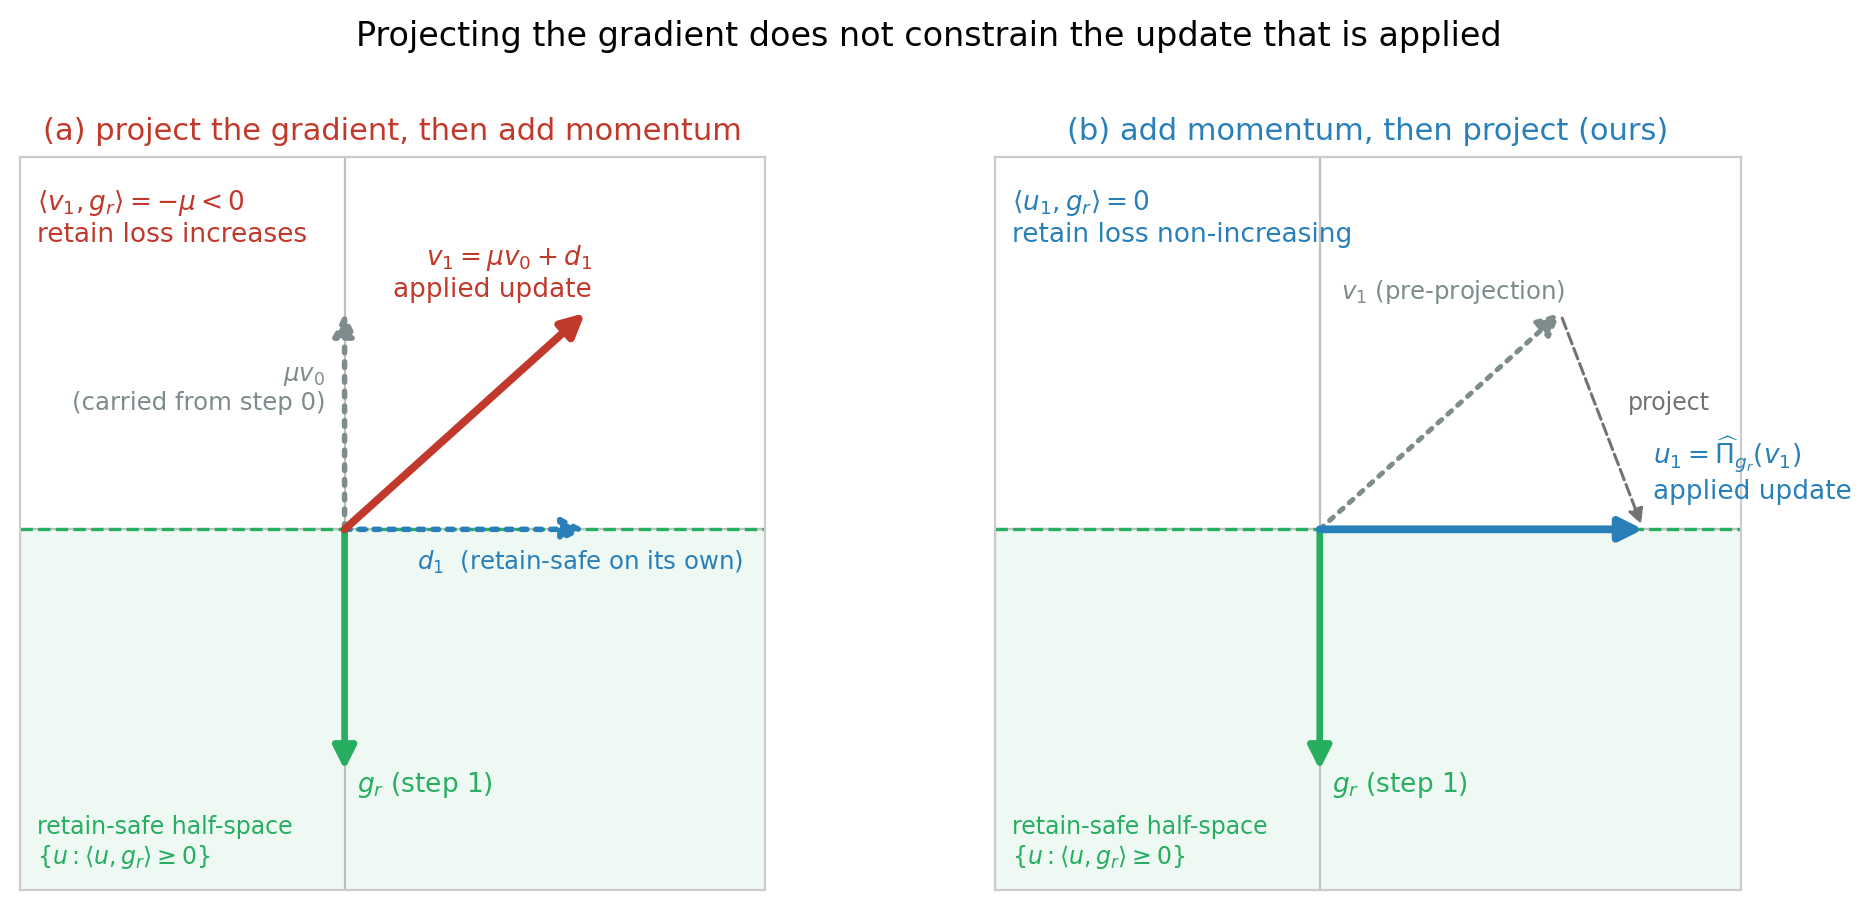
\includegraphics[width=0.86\textwidth]{fig_projection_order.png}
\caption{\textbf{Why the projection is applied to the update, not the
gradient} (Proposition~\ref{prop:counter}). Both panels show step~1, whose
constraint is $\gr$; the retain-safe half-space is shaded. \textbf{(a)}~Each
ingredient is individually retain-safe---$d_1$ lies on the boundary, and
$\mu v_0$ was certified against step~0's constraint---yet their sum, the vector
actually applied, lies in the harming half-space with
$\langle v_1,\gr\rangle = -\mu$. The violation grows with $\mu$.
\textbf{(b)}~Projecting the accumulated update instead returns it to the
boundary, so the certificate is issued against the constraint in force where
the step is taken.}
\label{fig:projorder}
\end{figure}

\subsection{Forget Objective, Stopping, and Normalisation}\label{sec:forget_obj}

The \klr{} objective drives forget-set predictions toward the retain-confusion
distribution rather than the uniform one,
\begin{equation}\label{eq:kl_retain}
\mathcal{L}_{\text{KL-R}} = \KL\!\left(\log\sigma(f_\theta(x_f)) \,\|\, p_r\right).
\end{equation}
Under the projected-momentum optimiser it forgets further than gradient ascent
\rev{and slightly further than a uniform target at equal test accuracy (FA
$2.1\%$ against $8.2\%$ and $3.9\%$, at TA $86.1$, $86.4$ and $86.4\%$; CIFAR-10
class~0, one seed)} and is within noise of a uniform target on MIA, so we claim a
better forget \emph{direction}, not a closer imitation of a retrained model
(Appendix~\ref{app:method}).

\paragraph{Dual stopping.}\label{sec:stopping}
Unlearning halts if the retain \rev{cross-entropy, measured on the full retain
set after each epoch,} exceeds $\alpha$ times its initial value, and completes
when FA reaches \rev{the target $\tau_F$}---by default the chance level
$100/K\%$---checked \rev{every $m=50$ steps} within epochs, because FA can fall
by tens of points inside one.

\paragraph{BatchNorm.}\label{sec:bn}
Class-homogeneous forget batches would corrupt BatchNorm running statistics, so
\ours{} freezes them. \added{The weights then learn to forget relative to those
frozen statistics; \S\ref{sec:bn_results} shows that this forgetting does not
survive recomputing them, and BN-robust \ours{} recomputes them from retained
data before every step instead (\S\ref{sec:bn_robust}).} A distillation anchor to
the frozen base model \rev{enters the retain objective; removing it changes
retain accuracy by only $0.04$pp on CIFAR-10 (\S\ref{sec:guarantee_measured}),
so we keep it as a safeguard rather than claim it as load-bearing}.

% ============================================================
\section{Theoretical Guarantees}\label{sec:theory}

\begin{theorem}[Exact per-step retain safety under momentum]\label{thm:retain_safety}
Let \rev{$\Lrt$, the retain objective $\lossr$ (cross-entropy plus
$\beta\losskd$) evaluated on the sampled retain mini-batch,} be $L$-smooth, and
let $\gr = \nabla_\theta\Lrt(\theta_t)$. Let \ours{} run the update of
Algorithm~\ref{alg:excise}: $\|d_t\| \le c$ by clipping,
$v_t = \mu v_{t-1} + d_t$ with $v_{-1}=0$ and $\mu \in [0,1)$,
$u_t = \Pi_{\gr}(v_t)\,\|v_t\|/\|\Pi_{\gr}(v_t)\|$ when
$\langle v_t,\gr\rangle<0$ \rev{(and $u_t=0$ if $\Pi_{\gr}(v_t)=0$)} and
$u_t = v_t$ otherwise, and $\theta_{t+1} = \theta_t - \eta u_t$. Then, exactly
and \rev{with no assumption on $\gf$ or on its alignment with $\gr$},
\begin{equation}\label{eq:thm1}
\langle u_t,\gr\rangle \ge 0,
\qquad \|u_t\| \;\rev{\le}\; \|v_t\| \;\le\; \frac{c}{1-\mu},
\qquad \Lrt(\theta_{t+1}) \;\le\; \Lrt(\theta_t) + \tfrac{1}{2}L\eta^2\Big(\frac{c}{1-\mu}\Big)^{\!2}.
\end{equation}
\end{theorem}

\begin{proof}[Proof sketch]
The first claim is immediate: if $\langle v_t,\gr\rangle \ge 0$ then $u_t=v_t$;
otherwise $\langle \Pi_{\gr}(v_t),\gr\rangle = 0$ identically, and rescaling by
a positive scalar preserves this. For the second, $\Pi_{\gr}$ is the orthogonal
projection onto $\{u : \langle u,\gr\rangle = 0\}$, so the rescaling restores
$\|u_t\|=\|v_t\|$ \rev{unless the projection vanishes}; unrolling the buffer gives
$v_t = \sum_{k=0}^{t}\mu^{t-k}d_k$, hence
$\|v_t\| \le c\sum_{j=0}^{t}\mu^{j} < c/(1-\mu)$. The third follows from
$L$-smoothness,
$\Lrt(\theta_{t+1}) \le \Lrt(\theta_t) - \eta\langle u_t,\gr\rangle
+ \tfrac{1}{2}L\eta^2\|u_t\|^2$, where the first-order term is non-positive by
claim one and $\|u_t\|$ is bounded by claim two. The full proof, together with the three supporting lemmas, is given in Appendix~\ref{app:thm1} (Theorem~\ref{thm:app_main}).
\end{proof}

The first-order change in the sampled retain loss is non-positive at every step,
and, unlike guarantees stated for momentum-free surrogates, the analysed $u_t$ is
the vector the code applies. The bound concerns the sampled mini-batch objective,
not the population retain loss (\S\ref{sec:limitations}).
\rev{Section~\ref{sec:guarantee_measured} tests the theorem on a logged run.}

\begin{theorem}[Per-step separation]\label{thm:separation}
For any model $\theta_0$ with retain gradient $\gr$:
\textbf{(i)}~GA's update $+\eta\gf$ strictly increases retain loss to first
order whenever $\langle\gf,\gr\rangle>0$;
\textbf{(ii)}~SCRUB's $-\gf+\lambda\gr$ can have $\langle\cdot,\gr\rangle<0$ for
any fixed $\lambda$;
\textbf{(iii)}~SalUn's masked random-label gradient has unconstrained sign with
respect to $\gr$;
\textbf{(iv)}~a soft conflict regulariser that adds $\rho\,\phi(\langle
g,\gr\rangle)$ with $\phi$ decreasing---the approach of the closest prior work
\citep{patel2025learning}---shifts the optimum toward positive alignment but
leaves the feasible set unrestricted: for any finite $\rho$, a sufficiently
large forget-loss reduction still makes a step with $\langle g,\gr\rangle<0$
preferable.
\rev{Among these update rules, only \ours{}'s} guarantees
$\langle u_t,\gr\rangle \ge 0$ \rev{at every step}, because only a projection
makes such steps unreachable rather than merely costly.
\end{theorem}

% ============================================================
\section{Experiments}\label{sec:experiments}

\subsection{Setup}\label{sec:setup}

We forget one class at a time on six benchmarks that vary class count, examples
per class and domain: CIFAR-10 and CIFAR-100 \citep{krizhevsky2009cifar}, MNIST
\citep{lecun1998mnist}, SVHN \citep{netzer2011svhn}, STL-10
\citep{coates2011stl10} and PathMNIST \citep{yang2023medmnist}. We forget every
class of MNIST and PathMNIST, \rev{classes $10, 20, \dots, 90$ of CIFAR-100}, and
class~0 of CIFAR-10, SVHN and STL-10 over three seeds: 31 tasks and 75 runs. All
models are ResNet-18 \citep{he2016resnet}. \rev{SalUn, SCRUB, Bad Teacher and
NegGrad+ are re-run on our stack, and a model retrained without the forget class
serves as the reference. MIA is the mean AUROC of a loss and a confidence
attack.} Hyperparameters are fixed per dataset and released as configuration
files (Appendix~\ref{app:hyper}); Appendix~\ref{app:experiments} gives the full
protocol. \rev{Table~\ref{tab:claims} lists every claim of \S\ref{sec:intro}
with the experiment that tests it; the subsections follow its order.}

\begin{table}[t]
\centering\color{revisedB}
\caption{\rev{\textbf{Each claim and the experiment that tests it.}}}
\label{tab:claims}
\small
\renewcommand{\arraystretch}{1.08}
\begin{tabular}{@{}>{\raggedright\arraybackslash}p{0.28\textwidth}>{\raggedright\arraybackslash}p{0.26\textwidth}>{\raggedright\arraybackslash}p{0.40\textwidth}@{}}
\toprule
\textbf{Claim} & \textbf{Test} & \textbf{Outcome} \\
\midrule
Forgets to chance, retain set intact & 31 tasks, six datasets (Table~\ref{tab:cross}) & Chance on all six, two at 60 epochs; RA $\ge 97.2\%$ on the 10-class datasets \\
Only \ours{} does both on CIFAR-10 & Four baselines, projection only (Table~\ref{tab:cifar10}) & FA $1.87\%$ at RA $100\%$; SalUn loses $2.9$pp RA, the rest stop at FA $\ge 18.7\%$ \\
Theorem~\ref{thm:retain_safety} holds for the optimiser that runs & Step-level audit (Figure~\ref{fig:guarantee}) & $120/120$ steps conflict before projection; $|\cos| \le 7.4\times10^{-7}$ after; $\|u_t\| \le 9.16 < 10$ \\
Soft corrections leave harm reachable (Thm.~\ref{thm:separation}) & Projection strength $s$, equal compute (\S\ref{sec:guarantee_measured}) & RA rises from $52.5$ to $99.98\%$ as $s \to 1$; every $s<1$ leaves conflict in the applied step \\
The projection protects the retain set & Ablation, equal compute (\S\ref{sec:guarantee_measured}) & Without it RA is $52.6\%$; alone it keeps RA $99.9\%$ but stops at FA $18.7\%$ \\
The guarantee must cover momentum & $\mu = 0$ ablation (Table~\ref{tab:momentum}) & With $\mu=0$, FA stays far above chance on five of six datasets \\
Frozen statistics make forgetting reversible & Recalibration attack (Table~\ref{tab:bnrecal}) & Frozen \ours{}: FA $1.4 \to 99.7\%$; base model and our baselines: $\Delta F \le 0$ \\
BN-robust \ours{} survives it & Ten classes, MNIST, attacker's data (Figures~\ref{fig:teaser}c, \ref{fig:bnrobust_attack}) & $|\Delta F| \le 0.06$pp on every CIFAR-10 class, $+0.09$pp on MNIST; attacker's data: $-1.2$ to $-1.0$pp \\
$0.5$ is the wrong MIA target & Retrained references (Table~\ref{tab:mia_main}) & References score $0.69$ (CIFAR-10) and $0.31$--$0.70$ (PathMNIST); rankings reverse \\
$p_r$ is a better direction than uniform & Forget objectives, equal TA (\S\ref{sec:forget_obj}) & FA $2.1\%$ against $3.9\%$ (uniform) and $8.2\%$ (GA); one seed \\
\bottomrule
\end{tabular}
\end{table}

\subsection{Main Results}\label{sec:main_results}

\begin{table}[t]
\centering
\caption{\textbf{Cross-dataset results.} Mean $\pm$ \rev{sample} std over
classes $\times$ seeds (3 seeds \rev{per task; one seed per class for
CIFAR-100}). \#T = number of forgetting tasks. Chance $=100/K\%$ is the level a
fully unlearned model must reach. \rev{The upper block uses each dataset's epoch
cap (12--20 epochs, Appendix~\ref{app:hyper}), which penalises datasets with few
images per class, since the binding resource is optimiser steps rather than
epochs. The lower block re-runs the two datasets that fall short at 60 epochs
($4\times$ and $3\times$ their caps), with a per-step check and a $1\%$ forget
target,} on the same seeds and classes;
$^*$marks the STL-10 row it supersedes (\S\ref{sec:crossdataset_stl}).}
\label{tab:cross}
\begin{tabular}{@{}lccccccc@{}}
\toprule
\textbf{Dataset} & \textbf{\#T} & \textbf{Chance} & \textbf{TA} & \textbf{FA}$\downarrow$ & \textbf{RA} & \textbf{MIA} \\
\midrule
CIFAR-10    & 1 & 10.0\% & $86.13 \pm 0.02$ & $\mathbf{1.87} \pm 0.25$ & $100.00 \pm 0.00$ & $0.529 \pm 0.001$ \\
MNIST       & 10 & 10.0\% & $90.00 \pm 0.64$ & $\mathbf{6.17} \pm 2.81$ & $99.49 \pm 0.04$ & $0.497 \pm 0.009$ \\
SVHN        & 1 & 10.0\% & $89.69 \pm 0.02$ & $\mathbf{5.75} \pm 0.17$ & $97.26 \pm 0.01$ & $0.525 \pm 0.001$ \\
STL-10$^*$  & 1 & 10.0\% & $92.84 \pm 0.02$ & $75.67 \pm 1.70$ & $99.38 \pm 0.10$ & $0.466 \pm 0.005$ \\
PathMNIST   & 9 & 11.1\% & $80.96 \pm 5.39$ & $\mathbf{5.82} \pm 3.42$ & $98.88 \pm 0.31$ & $0.483 \pm 0.084$ \\
CIFAR-100   & 9 & \phantom{0}1.0\% & $76.17 \pm 0.86$ & $4.07 \pm 5.51$ & $92.19 \pm 0.84$ & $0.500 \pm 0.037$ \\
\midrule
\multicolumn{7}{@{}l}{\emph{Extended budget} (\rev{60 epochs, per-step check, $1\%$ forget target}; same seeds and classes)} \\
STL-10      & 1 & 10.0\% & $85.15 \pm \rev{0.06}$ & $\mathbf{1.73} \pm \rev{0.95}$ & $98.87 \pm \rev{0.05}$ & $\rev{0.488} \pm \rev{0.008}$ \\
CIFAR-100   & 9 & \phantom{0}1.0\% & $75.50 \pm \rev{0.68}$ & $\mathbf{1.27} \pm \rev{0.39}$ & $91.32 \pm \rev{0.94}$ & $\rev{0.490} \pm \rev{0.043}$ \\
\bottomrule
\end{tabular}
\end{table}

\begin{table}[t]
\centering
\caption{\textbf{CIFAR-10 class-0 forgetting.} \ours{} is a 3-seed mean $\pm$
std. Methods with FA~$>80\%$ attain MIA~$\approx 0.5$ trivially, by barely
changing the model. $\dagger$Our reproduction; $\ddagger$our reproduction with
unified MIA. $^\S$A-GEM projection applied to plain gradient ascent, with
\ours{}'s KD anchor and retain-confusion target removed: the direct
projected-gradient baseline, isolating what the projection alone achieves.
\rev{$^\P$The retrained reference of \S\ref{sec:mia_main}; its TA and RA were
not logged, and its MIA, from the same two attacks, is $0.565$, not $0.5$.}}
\label{tab:cifar10}
\begin{tabular}{@{}lcccc@{}}
\toprule
\textbf{Method} & \textbf{TA} & \textbf{FA}$\downarrow$ & \textbf{RA} & \textbf{MIA} \\
\midrule
\rev{Retrain (reference)$^\P$} & \rev{---} & 0.0 & \rev{---} & \rev{0.565} \\
\midrule
SalUn$^\dagger$        & 84.0 & 0.0  & 97.1 & 0.497 \\
Bad Teacher$^\ddagger$ & 82.0 & 29.7 & 90.2 & 0.499 \\
SCRUB$^\ddagger$       & 93.3 & 88.8 & 97.7 & 0.515 \\
NegGrad+$^\ddagger$    & 94.2 & 84.8 & 99.3 & 0.525 \\
\midrule
Projection-only$^\S$   & 86.23 & 18.66 & 99.90 & 0.511 \\
\midrule
\textbf{\ours{}} & $\mathbf{86.13}\pm.02$ & $\mathbf{1.87}\pm.25$ & $\mathbf{100.00}\pm.00$ & $\mathbf{0.529}\pm.001$ \\
\bottomrule
\end{tabular}
\end{table}

\rev{At its epoch cap} \ours{} drives FA to or below the chance level on four
of six datasets with RA $\ge 97.2\%$ (CIFAR-100: $92.2\%$), and \rev{the mean
over seeds is below chance for every one of the ten MNIST and nine PathMNIST
classes (one of the 30 MNIST runs ends at $10.2\%$, within sampling error)}
(Table~\ref{tab:cross}, Appendix~\ref{app:perclass}). The two shortfalls are
budget-limited: STL-10 gets ${\sim}60$ optimiser steps at \rev{its 15-epoch cap}
against ${\sim}600$ for CIFAR-10 \rev{at the same cap}, and at 60 epochs
\rev{(per-step check, $1\%$ target)} STL-10 reaches $1.73\%$ \rev{($9.2\%$ in a
single run at its default $10\%$ target)} and CIFAR-100 $1.27\%$\rev{---against a $1\%$ chance level,
within one standard error of a 500-image forget set}---so all six datasets reach
chance. On CIFAR-10 (Table~\ref{tab:cifar10}, \rev{Figure~\ref{fig:teaser}b}),
\ours{} is the only method \rev{in the table} that both forgets to chance
and leaves retain accuracy untouched: SalUn forgets fully but costs $2.9$pp of
retain accuracy, Bad Teacher stops at $29.7\%$ while damaging the model, and
SCRUB and NegGrad+ keep the model intact by barely forgetting. The projection
alone does not unlearn: applied to plain gradient ascent it preserves the retain
set but stalls at $18.66\%$, so the projection supplies retain safety and the
\klr{} objective supplies the forgetting.

\subsection{The Guarantees, Measured}\label{sec:guarantee_measured}

\begin{figure}[t]
\centering
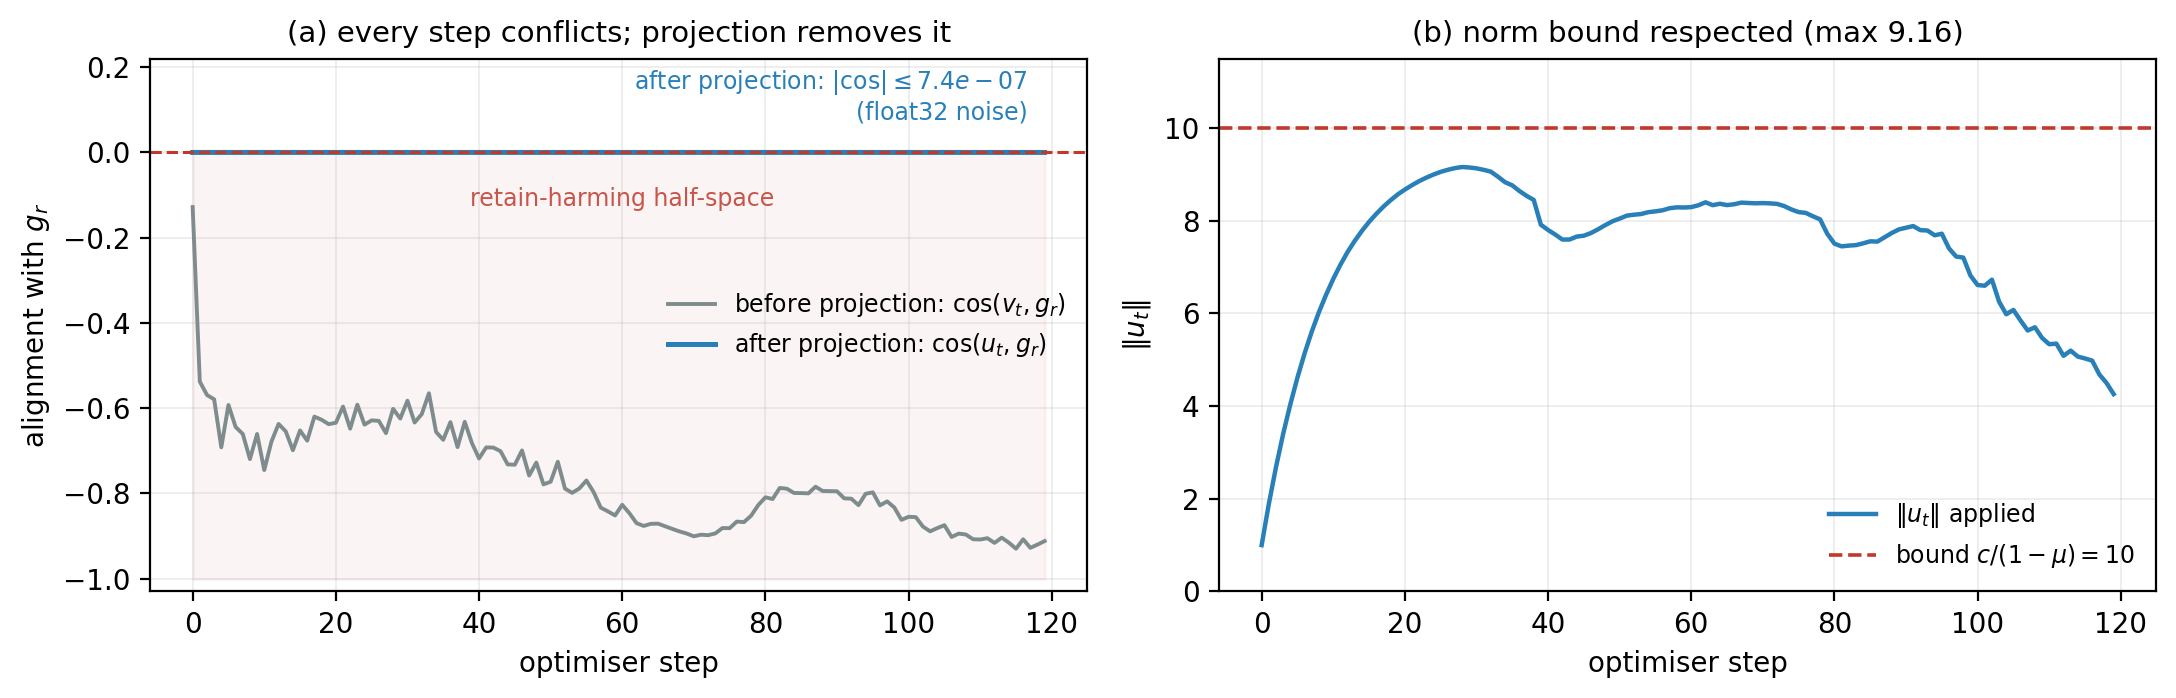
\includegraphics[width=0.86\textwidth]{fig_guarantee.png}
\caption{\textbf{Theorem~\ref{thm:retain_safety} audited on a real run}
(CIFAR-10 class~0, 120 steps). \textbf{(a)}~Alignment with the retain gradient,
normalised to $\cos(\cdot,\gr)$. Before projection every step lies in the
retain-harming half-space (mean $-0.77$); after projection the alignment is
indistinguishable from zero ($|\cos| \le 7.4\times10^{-7}$, the float32
accumulation scale). \textbf{(b)}~The applied update never exceeds the bound
$c/(1-\mu)=10$ of Eq.~\ref{eq:thm1}, peaking at $9.16$---tight, but respected.}
\label{fig:guarantee}
\end{figure}

\rev{\paragraph{Theorem~\ref{thm:retain_safety} on a real run.}
We log every step of a CIFAR-10 run (class~0, 120 steps;
Figure~\ref{fig:guarantee}, Appendix~\ref{sec:alignment}). The accumulated update
conflicts with the retain gradient at all 120 steps (mean
$\cos(v_t,\gr) = -0.77$), so the projection is the optimiser's defining step
rather than a safeguard. After projection the alignment is zero to float32
precision ($|\cos(u_t,\gr)| \le 7.4\times10^{-7}$), and $\|u_t\|$ peaks at
$9.16$ against the bound $c/(1-\mu)=10$.

\paragraph{Theorem~\ref{thm:separation}(iv): soft against hard.}
To test the separation without reimplementing another method, we vary our own
projection between a soft correction and the hard constraint: at conflicting
steps $u = v - s\,\frac{\langle v,\gr\rangle}{\|\gr\|^2}\gr$, so
$\langle u,\gr\rangle = (1-s)\langle v,\gr\rangle < 0$ for every $s<1$. At equal
compute with stopping disabled every setting forgets completely (FA $0.0\%$), so
the settings differ only in collateral damage: RA is $52.5$, $81.4$, $92.8$,
$98.2$ and $99.98\%$ for $s = 0, 0.25, 0.5, 0.75, 1$ (Appendix~\ref{sec:strength}).
The curve is gradual---$s=0.75$ already keeps $98.2\%$---so the case for $s=1$
is that it is the only setting with a guarantee, not that the last $1.8$pp is
large.

\paragraph{The projection is what protects the retain set.}
At equal compute with stopping disabled, removing the projection collapses the
model (TA $44.4\%$ and RA $52.6\%$, against $85.7\%$ and $99.98\%$ with it),
removing the distillation anchor changes RA by $0.04$pp, and the projection on
its own keeps RA at $99.9\%$ but stalls at FA $18.7\%$
(Tables~\ref{tab:cifar10} and~\ref{tab:ablation}). With stopping enabled every
variant halts after one epoch and the projection looks costless, which is why we
report both modes.}

\subsection{Momentum Is Not Incidental}\label{sec:momentum_ablation}

\begin{table}[t]
\centering
\caption{\textbf{Momentum ablation.} Removing momentum to simplify the analysis
\rev{leaves forget accuracy far above chance on five of six datasets; on STL-10
projected momentum also falls short at this budget (Table~\ref{tab:cross})}.
High RA with high FA indicates the model barely changed. Same configs, seeds,
and stopping rules throughout.}
\label{tab:momentum}
\begin{tabular}{@{}lccccc@{}}
\toprule
& & \multicolumn{2}{c}{$\mu=0$ (analysis-friendly)} & \multicolumn{2}{c}{Projected momentum (ours)} \\
\cmidrule(lr){3-4}\cmidrule(lr){5-6}
\textbf{Dataset} & \textbf{Chance} & \textbf{FA}$\downarrow$ & \textbf{RA} & \textbf{FA}$\downarrow$ & \textbf{RA} \\
\midrule
CIFAR-10  & 10.0\% & \phantom{0}5.8 & 100.0 & \phantom{0}1.9 & 100.0 \\
MNIST     & 10.0\% & 95.9 & \phantom{0}99.5 & \phantom{0}6.2 & 99.5 \\
SVHN      & 10.0\% & 61.9 & \phantom{0}97.4 & \phantom{0}5.8 & 97.3 \\
STL-10    & 10.0\% & 99.7 & \phantom{0}99.4 & 75.7 & 99.4 \\
PathMNIST & 11.1\% & 16.4 & \phantom{0}99.0 & \phantom{0}5.8 & 98.9 \\
CIFAR-100 & \phantom{0}1.0\% & 73.7 & \phantom{0}94.1 & \phantom{0}4.1 & 92.2 \\
\bottomrule
\end{tabular}
\end{table}

Removing momentum is the most direct route to an exact guarantee, since the
applied update then equals the projected gradient. Table~\ref{tab:momentum} shows
the cost: with $\mu = 0$ and everything else fixed, \rev{forget accuracy stays
far above chance on five of six datasets} (FA $95.9\%$ on MNIST, $99.7\%$ on
STL-10, $73.7\%$ on CIFAR-100), and RA stays high only because the model barely
moves. \rev{STL-10 does not forget at this budget with momentum either
($75.7\%$), so the comparison rests on the other four: without momentum all four
stay far above chance; with it, three reach chance and CIFAR-100 ends at
$4.1\%$.} A guarantee stated for the momentum-free update would be exact and
would describe a method that does not unlearn. The dependence is not ours alone:
every update rule we tested loses forgetting without momentum, but the KL
objectives lose $70$--$79$pp against $12$--$15$pp for gradient ascent \rev{(with
or without projection; means over MNIST and SVHN), consistent with a bounded
objective needing} momentum's $1/(1-\mu)$ amplification
(Appendix~\ref{app:momentum}).

\subsection{BatchNorm: the Attack, and a Fix That Keeps BatchNorm}\label{sec:bn_results}

\begin{table}[t]
\centering
\caption{\textbf{BatchNorm recalibration} (CIFAR-10, class~0), using
\texttt{update\_bn} on the retain set: BatchNorm buffers are reset and
recomputed, no weight is touched. \rev{Our reproductions of the baselines}
and the un-unlearned base model are unaffected ($\Delta F \le 0$); \ours{} with a
BatchNorm backbone loses essentially all of its forgetting. The two backbones without running statistics
are outside the operator's reach by construction. NegGrad+ is omitted: no
checkpoint for it was available.}
\label{tab:bnrecal}
\begin{tabular}{@{}lccccc@{}}
\toprule
Configuration & pre-$F$ & post-$F$ & $\boldsymbol{\Delta F}$ & pre-TA & post-TA \\
\midrule
Base model (no unlearning)  & $100.0$ & $99.8$ & $-0.2$ & $95.5$ & $92.9$ \\
SalUn                       & $0.0$   & $0.0$  & $+0.0$ & $84.7$ & $84.4$ \\
Bad Teacher                 & $28.7$  & $28.4$ & $-0.3$ & $81.5$ & $84.0$ \\
SCRUB                       & $89.3$  & $85.7$ & $-3.6$ & $93.5$ & $93.2$ \\
\midrule
\ours{} (BatchNorm, frozen) & $1.4$   & $99.7$ & $\mathbf{+98.4}$ & $86.1$ & $92.9$ \\
\ours{} (GroupNorm)         & $4.9$   & $4.9$  & $\mathbf{0.0}$   & $84.2$ & $84.2$ \\
\ours{} (ViT-B/16, LayerNorm) & $9.6$ & $9.6$  & $\mathbf{0.0}$   & $87.0$ & $87.0$ \\
\bottomrule
\end{tabular}
\end{table}

\begin{table}[t]
\centering\color{revised}
\caption{\added{\textbf{BN-robust \ours{} under BatchNorm recalibration} (CIFAR-10,
class~0, seeds $\{42,123,456\}$; \texttt{update\_bn} on the retain set, as in
Table~\ref{tab:bnrecal}). Every row shares the $93.97\%$ base except GroupNorm,
which needs its own. The un-unlearned base is the control: recalibrating it
changes nothing. \emph{Naive} stopping reads FA under the in-loop statistics,
\emph{calibrated} stopping under the statistics that ship. Time is wall-clock per
run on one GPU.}}
\label{tab:bnrobust}
\small
\setlength{\tabcolsep}{4pt}
\begin{tabular}{@{}lcccccccc@{}}
\toprule
Configuration & base TA & pre-$F$ & post-$F$ & $\boldsymbol{\Delta F}$ & TA & RA & epochs & min \\
\midrule
Base model (no unlearning)     & $93.97$ & $99.80$ & $99.82$ & $+0.0$ & $93.97$ & ---     & ---          & ---    \\
\ours{} (BatchNorm, frozen)    & $93.97$ & $8.51 \pm 0.30$  & $99.12 \pm 0.09$ & $\mathbf{+90.6}$ & $85.20$ & $97.34$ & $2$          & $1.9$  \\
\ours{} (GroupNorm)            & $91.89$ & $5.91 \pm 0.09$  & n/a              & n/a              & $83.13$ & $98.92$ & $3$          & $2.5$  \\
BN-robust, naive stopping      & $93.97$ & $11.43 \pm 1.90$ & $11.44 \pm 1.87$ & $\mathbf{0.0}$   & $84.42$ & $95.46$ & $11$--$13$   & $9.8$  \\
BN-robust, calibrated stopping & $93.97$ & $9.19 \pm 0.08$  & $9.18 \pm 0.07$  & $\mathbf{0.0}$   & $84.30$ & $95.59$ & $13$         & $13.3$ \\
\bottomrule
\end{tabular}
\end{table}

\paragraph{The attack.}
\texttt{update\_bn} resets every BatchNorm buffer and recomputes the statistics
on the retain set without touching a weight; we verify that every learnable
parameter is bit-identical afterwards. Table~\ref{tab:bnrecal} shows that
recalibration leaves the un-unlearned base model and every baseline we
reproduced unaffected, but undoes \ours{} with frozen statistics completely:
forget accuracy returns from $1.4\%$ to $99.7\%$ and test accuracy to $92.9\%$,
\rev{the value recalibration gives the base model itself}. Because the
statistics are frozen, the weights learn to forget against statistics an
attacker can replace. \rev{Our baseline reproductions survive because each ends
every epoch with a pass over retained data in train mode, which recomputes the
statistics. Under their reference implementations, \citet{kalani2026batchnorm}
recover six of nine prior methods, and find SalUn's recovery disappears once at
least a quarter of each unlearning batch is retained data.} GroupNorm and a ViT's
LayerNorm keep no running statistics and are outside the attack's reach by
construction (Tables~\ref{tab:gn} and~\ref{tab:vit}), but that is a change of
architecture, not robustness.

\paragraph{BN-robust \ours{}.}\label{sec:bn_robust}
\added{We keep BatchNorm and stop the statistics going stale. Before every step
they are recomputed on 512 retain images with the attacker's own operator, after
the last step on the whole retain set, and the stopping rule reads forget
accuracy under the statistics that will ship, falling back to the best epoch if
the target is not met (\rev{Figure~\ref{fig:bnrobust_mech}, Appendix~\ref{app:bn_robust}}). The update rule is
unchanged, \rev{so Theorem~\ref{thm:retain_safety} holds at every step for the
retain objective under the statistics in force during that step; the
recalibration between steps is not a gradient step, and the theorem does not
bound its effect}. Table~\ref{tab:bnrobust} gives the
result on a separate base model (the checkpoints behind Table~\ref{tab:bnrecal}
were no longer available): with frozen statistics the attack returns forget
accuracy to $99.1\%$, while BN-robust \ours{} forgets to $9.2\%$ and stays at
$9.2\%$. It holds on all ten CIFAR-10 classes ($6.7$--$10.2\%$ after the attack,
all within three standard errors of chance), on MNIST ($3.9\%$, where frozen
statistics recover to $99.97\%$), and when the attacker recalibrates on the full
training set or the test set instead \rev{(tested on the naive-stopping
checkpoints, whose FA moves by $-1.2$ to $-1.0$pp)} (Figure~\ref{fig:bnrobust_attack},
Appendix~\ref{app:bn_robust}). It costs
about seven times the compute and $1.8$pp of retain accuracy, mostly because
forgetting that must happen in the weights takes ${\sim}13$ epochs
instead of~$2$.}

\begin{figure}[t]
\centering\color{revised}
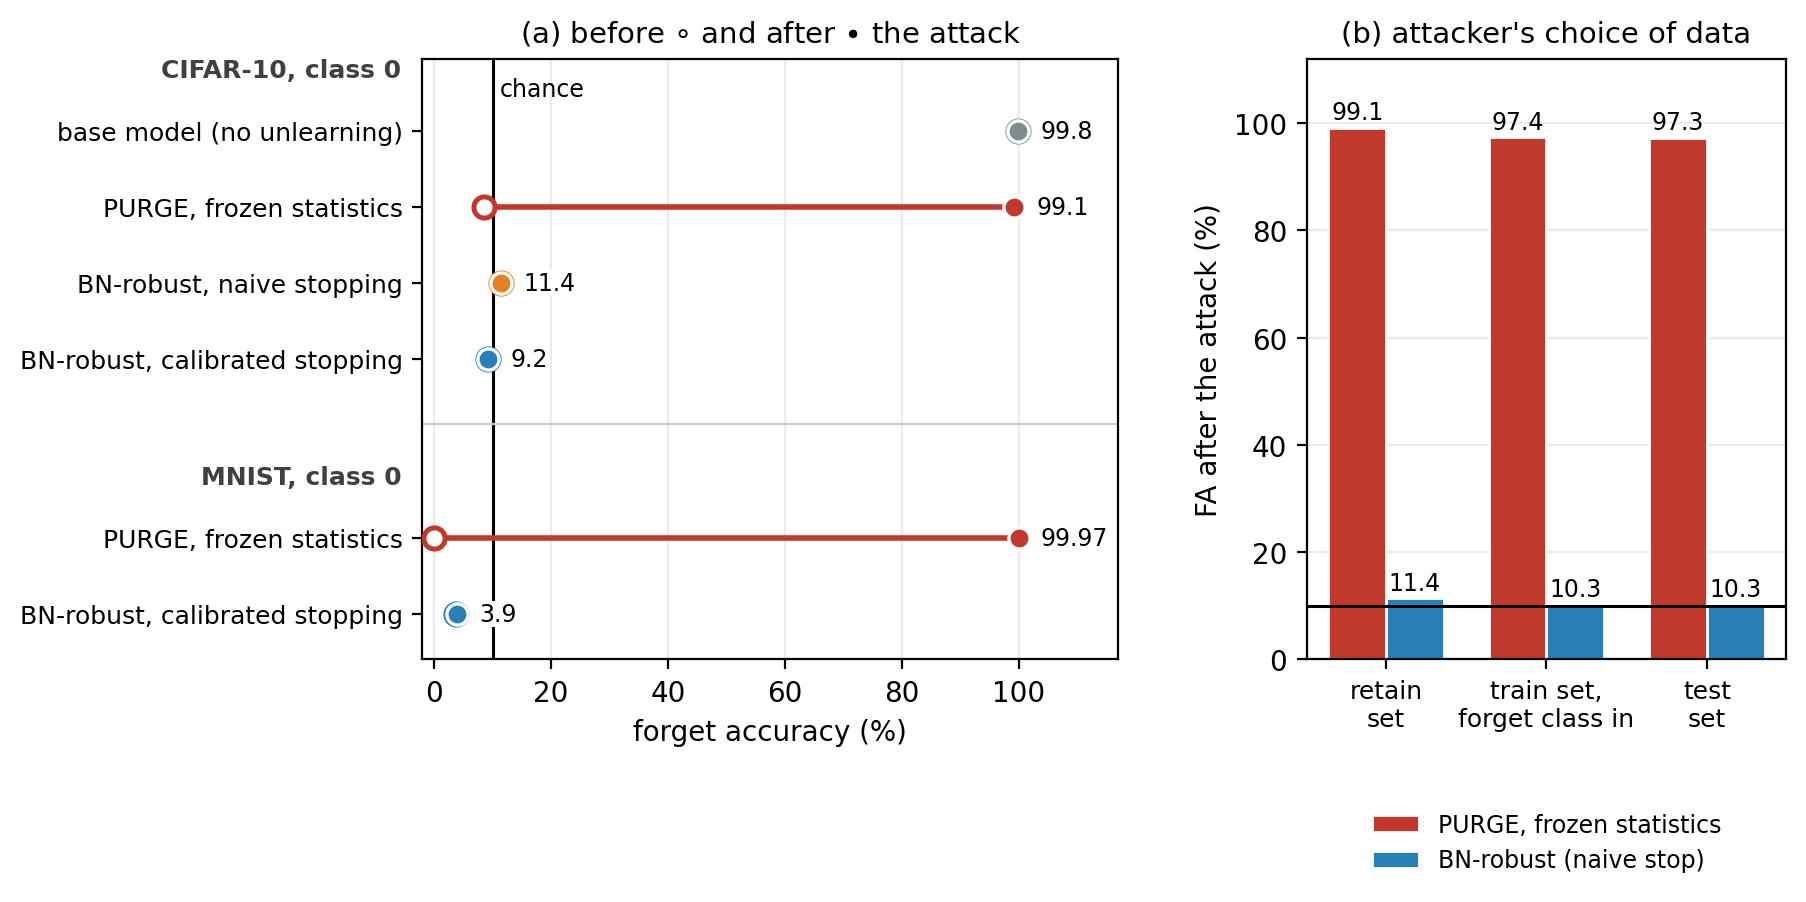
\includegraphics[width=\textwidth]{fig_bnrobust_attack.png}
\caption{\added{\textbf{BN-robust survives the recalibration attack.} (a)~Forget
accuracy before (open) and after (filled) \texttt{update\_bn} on the retain set,
class~0, means over three seeds; on MNIST the frozen configuration's forgetting
is undone completely. (b)~Forget accuracy after the attack when the attacker
recalibrates on the retain set, the full training set (forget class included),
or the test set (CIFAR-10 class~0, three seeds; BN-robust with naive stopping).}}
\label{fig:bnrobust_attack}
\end{figure}

\subsection{Membership Inference Needs a Retrained Reference}\label{sec:mia_main}

\rev{MIA is usually read against $0.5$: an attacker should not be able to tell
forget-class training samples from forget-class test samples. We test that
target against models retrained without the forget class, which trained on
neither group (Table~\ref{tab:mia_main}; Appendix~\ref{sec:mia} adds three
attacks). On CIFAR-10 the reference scores $0.694$ on the loss attack, with a
true-positive rate of $12.5\%$ at $1\%$ false positives, while the base model,
which memorised every member, scores $0.483$: the attack reads a difference in
difficulty between the train and test splits, not membership. Across four
PathMNIST classes the reference ranges from $0.306$ to $0.704$, so no single
constant is the right target. Read against $0.5$, \ours{} looks the worst of the
four methods on CIFAR-10 and SalUn the best; read against the reference, the
order reverses. SalUn's $0.500$ is also degenerate: its true-positive rate is
zero at every threshold, the signature of a constant score. On three of the four
PathMNIST classes \ours{} sits far from its own reference (mean gap
$0.22$--$0.36$ over four attacks), so we claim the protocol finding, not that
\ours{} matches retrained models in general.}

\begin{table}[t]
\centering\color{revisedB}
\caption{\rev{\textbf{Loss-attack MIA against a retrained reference}
(CIFAR-10, class~0). Members are the $5000$ forget-class training images,
non-members the $1000$ forget-class test images; TPR is at $1\%$ FPR.
Appendix~\ref{sec:mia} gives three further attacks and four PathMNIST classes.}}
\label{tab:mia_main}
\small
\begin{tabular}{@{}lccccc@{}}
\toprule
Model & FA & AUROC & TPR & $|\mathrm{AUROC}-0.5|$ & $|\mathrm{AUROC}-\mathrm{ref}|$ \\
\midrule
Retrained (reference) & $0.0$   & $0.694$ & $12.5\%$ & $0.194$ & ---   \\
Base (no unlearning)  & $100.0$ & $0.483$ & $0.0\%$  & $0.017$ & $0.211$ \\
\midrule
SalUn                 & $0.0$   & $0.500$ & $0.0\%$  & $\mathbf{0.000}$ & $0.194$ \\
Bad Teacher           & $24.8$  & $0.485$ & $0.2\%$  & $0.015$ & $0.209$ \\
SCRUB                 & $89.5$  & $0.477$ & $0.4\%$  & $0.023$ & $0.217$ \\
\ours{}               & $2.0$   & $0.693$ & $1.4\%$  & $0.193$ & $\mathbf{0.001}$ \\
\bottomrule
\end{tabular}
\end{table}

\subsection{Further Analyses}\label{sec:further}

The appendices report the remaining experiments in full. \emph{Transformer:} on
ViT-B/16 forgetting transfers \rev{on CIFAR-10}, with FA $9.71\%$ and RA
$97.55\%$, \rev{but not on CIFAR-100 within its 20-epoch cap, where FA ends
between $4.0\%$ and $82.0\%$ across nine classes against a $1\%$ chance level}
(Appendix~\ref{sec:vit}). \emph{Tolerances:} the retain budget is non-binding,
and the forget target is a usable knob over a $29$pp range once it is checked at
every step (Appendix~\ref{sec:sweeps}). \emph{Distance to a retrained model:}
\ours{} is closest in feature space (Fr\'echet distance $13$ against
$153$--$495$ for the baselines) and SalUn in output space
(Appendix~\ref{sec:distance}). \emph{Stopping point:} divergence to a retrained
model is U-shaped along the trajectory with its minimum above chance, and MIA
passes through $0.5$ rather than converging to it
(Appendices~\ref{sec:overforget} and~\ref{sec:trajectory}). \rev{\emph{Sequential
unlearning:} over three classes TA falls from $86.1\%$ to $69.1\%$ and RA from
$100\%$ to $80.7\%$, no more than the forgotten classes themselves account for
(\S\ref{sec:limitations}).}

% ============================================================
\section{Limitations}\label{sec:limitations}

The compute a dataset needs cannot be predicted in advance: the binding resource
is optimiser steps, and STL-10 and CIFAR-100 needed 60 epochs rather than 15 and
20\rev{; ViT-B/16 on CIFAR-100 does not reach chance within its 20-epoch cap}.
Sample-level forgetting works only crudely, because the retain-confusion
target degenerates to uniform when every class remains in the retain set. The
guarantee bounds the sampled mini-batch retain objective, not the population
loss, and holds to float32 precision\rev{; under BN-robust \ours{} it holds per
step under that step's statistics and does not cover the recalibration between
steps}. Our separation from soft conflict-resolution methods
\citep{patel2025learning} is structural; we have not run that method on our
stack. BN-robust \ours{} costs about seven times the compute, was evaluated on
two datasets, and defends only the normalisation statistics, not weight-level
attacks such as fine-tuning recovery\rev{; its comparison with prior methods
rests on the evaluations of \citet{kalani2026batchnorm} and on our own
reproductions, and a like-for-like run of those methods under the same base and
attack remains to be done. In sequential unlearning the retained classes are not
damaged cumulatively, but earlier-forgotten classes partly return: after three
classes RA is $80.7\%$, above the $77.8\%$ that fully forgotten classes would
allow, so they average at least $13\%$ training accuracy, above chance.} \ours{}
gives no differential-privacy guarantee. Appendix~\ref{app:limitations}
discusses each point.

% ============================================================
\section{Conclusion}\label{sec:conclusion}

Unlearning is the dual of continual learning, and \rev{one of continual
learning's most direct tools, a hard constraint on the update, carries over}.
For that constraint to mean anything it must be stated for the update the
optimiser applies: projecting the post-momentum update makes
Theorem~\ref{thm:retain_safety} exact for the deployed optimiser, while the
analysis-friendly alternative \rev{leaves forget accuracy far above chance on
five of six datasets}. Across six datasets and 31 forgetting tasks \ours{}
reaches the chance level on all six (two at a longer budget) with retain
accuracy at or above $97.2\%$ on the 10-class datasets, and \rev{step-level logs
of a CIFAR-10 run} confirm the constraint at every step.
\added{On BatchNorm backbones, keeping the normalisation statistics consistent
with the weights throughout unlearning makes that forgetting survive
recalibration, on every CIFAR-10 class and on MNIST.} The duality is also a
design space: \rev{many continual-learning techniques that protect old-task
knowledge suggest unlearning counterparts} that protect retained knowledge
during erasure. More broadly, when an
optimiser detail is chosen for analytical convenience, it should be checked
against the behaviour it was meant to explain.

\FloatBarrier
% tmlr.bst when available; plainnat keeps the document compilable without it.
\IfFileExists{tmlr.bst}{\bibliographystyle{tmlr}}{\bibliographystyle{plainnat}}
\bibliography{../references}

% ============================================================
\appendix
% ============================================================
\section{Related Work and Positioning in Full}\label{app:related}\label{sec:related_intro}

Approximate unlearning methods occupy different points on the privacy--utility
frontier, and the retain side is where they differ most. \textbf{Gradient
ascent} \citep{thudi2022unrolling} maximises forget-set loss with no mechanism
protecting retain accuracy \rev{(Theorem~\ref{thm:separation}(i))}. \textbf{SalUn} \citep{fan2024salun} confines random-label updates to a
saliency mask---effective in practice, but with no formal retain guarantee and
no control over how much is forgotten. \textbf{SCRUB}
\citep{kurmanji2023unbounded} alternates forget and retain steps balanced by a
weight $\lambda$, so the balance is tuned rather than enforced; in our
reproduction it preserves retain accuracy ($97.7\%$) by barely forgetting at all
(forget accuracy $88.8\%$, Table~\ref{tab:cifar10}). \textbf{NegGrad+}
\citep{thudi2022unrolling} adds a retain-loss term as a weighted sum, again
without a guarantee that retain loss is controlled. Closest to us,
\citet{patel2025learning} diagnose the same forget--retain gradient conflict but
resolve it with a soft regulariser that rewards positive alignment. A fuller treatment, including exact unlearning and distillation-based methods, follows the table.

The distinction we draw is structural rather than numerical, so
Table~\ref{tab:properties} compares properties of each method's \emph{definition}
---checkable against the published update rule, without relying on our
reimplementation of it. A soft penalty biases the optimiser toward retain-safe
steps but leaves harmful steps feasible: for any finite penalty weight, a
sufficiently large forget-loss reduction still makes a retain-harming step
preferable. A projection removes those steps from the feasible set altogether
(Theorem~\ref{thm:separation}(iv)). The final row is the one we would emphasise,
and the one \S\ref{sec:momentum_ablation} makes concrete: a guarantee proved for
a momentum-free surrogate says nothing about a run that uses momentum.

\rev{Figure~\ref{fig:teaser}} places the method against the alternatives on both
what it achieves and what it guarantees.

\paragraph{Exact unlearning.}
SISA \citep{bourtoule2021sisa} partitions data into shards so that removal
requires retraining only the affected shard; the per-deletion cost approaches
full retraining as shard count grows. Certified removal
\citep{guo2020certified} gives exact guarantees for convex models but does not
extend to deep networks.

\paragraph{Gradient-based approximate unlearning.}
GA \citep{thudi2022unrolling} maximises forget-set loss, with no mechanism to
prevent the same direction from degrading retain performance. Amnesiac
unlearning \citep{graves2021amnesiac} subtracts cached per-sample updates,
requiring $O(T|\Df|)$ storage. NegGrad+ optimises
$-\lossf + \lambda\lossr$ directly, which is the Lagrangian relaxation of
Eq.~\ref{eq:problem} rather than a solution to it: the retain term shifts the
optimum without bounding any single step, so the weighted sum is exactly the
soft treatment Theorem~\ref{thm:separation}(iv) separates us from.

\paragraph{Saliency and Fisher methods.}
SalUn \citep{fan2024salun} applies random-label updates inside a top-50\%
saliency mask: strong empirically (FA~$=0\%$ on CIFAR-10) but with no formal
retain guarantee and no control over the degree of forgetting. Fisher-based
methods \citep{golatkar2020eternal,golatkar2021scrubbing} and SSD
\citep{foster2024ssd} weight parameters by estimated importance, requiring
Hessian approximations that scale poorly.

\paragraph{Knowledge distillation.}
Bad Teacher \citep{chundawat2023badteacher} uses competent/incompetent teachers.
SCRUB \citep{kurmanji2023unbounded} is closest in motivation---both draw on CL
intuitions and use KD to anchor retain behaviour---but differs algorithmically:
SCRUB alternates forget and retain steps balanced by $\lambda$, so its balance is
hyperparameter-dependent, whereas \ours{}'s retain safety holds by construction
(Theorem~\ref{thm:separation}); and SCRUB ascends the forget loss, which is
unstable in either direction, whereas \klr{} converges to a specific target
distribution.

\paragraph{Continual learning connection, and the closest prior work.}
A-GEM \citep{chaudhry2019agem} projects task gradients to avoid catastrophic
forgetting. The CL--MU duality has been noted conceptually
\citep{nguyen2020variational,kurmanji2023unbounded}. Closest to \ours{}, recent
work \citep{patel2025learning} also targets the forget--retain gradient
conflict, but through an \emph{implicit, soft} regulariser encouraging a positive
inner product---with no per-step constraint and no formal guarantee. More
broadly, gradient projection and conflict resolution are now actively explored
for unlearning. \added{Closest in mechanism is Projected-Gradient Unlearning
\citep{hoang2024learn}, which takes unlearning steps orthogonal to a gradient
subspace estimated for the retained data. \ours{} differs in the constraint and in
what it binds: a half-space against the current retain gradient---the minimum
correction that excludes retain-harming steps---applied to the post-momentum
update the optimiser actually takes.} \ours{} enforces $\langle u_t,\gr\rangle \ge 0$ explicitly at every
step, on the post-momentum update, which is the difference between \emph{softly
discouraging} conflict and \emph{provably eliminating} it---and, relative to
guarantees stated for momentum-free surrogates, the difference between a bound
that describes the deployed optimiser and one that does not.
\S\ref{sec:strength} tests the mechanism this distinction rests on by varying
our own projection between a soft penalty and the hard constraint; a
like-for-like run of that method on our stack remains future work.

% ============================================================
\section{Design Details}\label{app:method}

\subsection{From the Optimisation Problem to the Algorithm}

This framing makes three things explicit that weighted multi-objective
approaches conflate. First, retain safety is a \emph{hard constraint}, not a
soft penalty. Second, \rev{the forget objective sets the direction of the
search and the forget-accuracy target its end point; only the second is a
constraint}. Third, the two tolerances \rev{$(\alpha, \tau_F)$} are quantities a
practitioner sets, not epochs to be tuned.

\paragraph{Why this needs a new algorithm.} Writing down
Eq.~\ref{eq:problem} is not by itself progress: one could hand it to a generic
constrained solver, or relax it into the weighted objective that existing
methods already optimise. Both routes lose the property we are after. A
Lagrangian relaxation replaces the retain constraint with a penalty
$\lambda\,\lossr$, which is precisely the soft treatment whose feasible set still
contains retain-harming steps (Theorem~\ref{thm:separation}(iv)); and a
projected-gradient solver applied naively would enforce feasibility on the
gradient while the optimiser applies something else
(Proposition~\ref{prop:counter}). What the problem \emph{does} buy is a
specification: it says exactly which quantity each mechanism must control.
\rev{\ours{} realises each condition with the cheapest mechanism we know that
enforces it, and enforces retain safety at every step on the vector actually
applied.} Table~\ref{tab:constraint_map} states that correspondence, and
\S\ref{sec:method} derives each row.

\begin{table}[t]
\centering
\caption{\rev{\textbf{From the problem to the algorithm.} Each condition of
Eq.~\ref{eq:problem}, and the property of the search path, with the mechanism
that enforces it. Two components serve no condition directly: the distillation
anchor, which is part of the retain objective the projection protects, and the
handling of BatchNorm statistics (\S\ref{sec:bn}).}}
\label{tab:constraint_map}
\color{revisedB}
\begin{tabular}{@{}p{0.31\textwidth}p{0.33\textwidth}p{0.28\textwidth}@{}}
\toprule
\textbf{Condition} & \textbf{Mechanism} & \textbf{Enforced} \\
\midrule
Retain objective does not increase along the path &
Projection of the post-momentum update onto $\{\langle u,\gr\rangle \ge 0\}$ (\S\ref{sec:projection}--\ref{sec:optimiser}) &
Every step, to first order on the sampled batch (Thm.~\ref{thm:retain_safety}) \\
\addlinespace
$\CE(\theta;\Dr) \le \alpha\,\CE(\theta_0;\Dr)$ &
Retain-loss stopping rule (\S\ref{sec:stopping}) &
After every epoch, on the full retain set \\
\addlinespace
$\mathrm{FA}(\theta;\Df) \le \tau_F$ &
Forget-accuracy stopping rule (\S\ref{sec:stopping}) &
Every $m$ steps \\
\addlinespace
Direction of the search &
\klr{}: descend $\KL(p_\theta(x_f)\|p_r)$ (\S\ref{sec:forget_obj}) &
Every step \\
\addlinespace
$\|\theta - \theta_0\| \le R$ &
Clipping before accumulation, and the step budget &
$\|\theta_N - \theta_0\| \le N\eta c/(1-\mu)$ \\
\bottomrule
\end{tabular}
\end{table}

\subsection{What Is Taken from A-GEM, and What Is Not}

The operator in
Eq.~\ref{eq:projection} is A-GEM's, and we claim no novelty for it: the
correction $v \mapsto v - \frac{\langle v,g\rangle}{\|g\|^2}g$ is the standard
projection onto a half-space, and \citet{chaudhry2019agem} introduced its use in
continual learning with $g$ the gradient on an episodic memory of past tasks. We
also inherit its two attractive properties: it is the \emph{minimum-norm}
correction restoring feasibility, so it is the least destructive repair of a
conflicting step, and it costs one extra backward pass and one inner product per
step.

What is new is what the operator is asked to do. In A-GEM the projection is a
safeguard on a process whose objective already points the right way---the new
task is being learned, and the memory gradient only occasionally interferes; in
our runs the conflict is not occasional but universal, firing at $100\%$ of
steps (\S\ref{sec:alignment}), because erasing a class and preserving the rest
are directly opposed rather than incidentally so. The projection is therefore
not a correction applied to an optimiser but the optimiser's defining step. That
change of role has three consequences, and they are what
\S\ref{sec:optimiser} is about:
\begin{enumerate}
\item \emph{It must bind the applied vector.} A-GEM projects a gradient; with
momentum the applied vector is not the gradient, and projecting the gradient
certifies nothing (Proposition~\ref{prop:counter}).
\item \emph{Its magnitude matters.} A-GEM tolerates $\|\Pi_{\gr}(v)\| \le \|v\|$
because progress on the new task comes mostly from unconflicted steps. When
every step conflicts, that contraction compounds and forgetting stalls, so we
restore the norm after projecting.
\item \emph{It bounds nothing on the forget side.} The projection guarantees
retain safety and only that; on its own it does not unlearn. Our projection-only
ablation reaches forget accuracy $18.66\%$ against a $10\%$ chance level
(Table~\ref{tab:cifar10}), which is why \ours{} pairs it with a forget objective
rather than presenting the projection as a method.
\end{enumerate}

\subsection{The Three Ordering Choices}

\ours{} uses SGD with momentum $\mu$, weight decay $\lambda_{\mathrm{wd}}$, and
gradient clipping $c$. Three ordering choices determine whether the guarantee is
real, and all three matter empirically.

\paragraph{(i) Project the update, not the gradient.}
The vector applied to the weights is $u_t$, not $\gf$. We therefore
momentum-accumulate first and project afterwards
(Algorithm~\ref{alg:excise}, lines 10--15), so that
$\langle u_t,\gr\rangle \ge 0$ holds for the update that is actually applied.
Projecting $\gf$ instead leaves $\langle u_t,\gr\rangle$ unconstrained.

\paragraph{(ii) Clip before accumulating.}
Clipping is applied to the per-step ingredient $d_t$ \emph{before} it enters the
momentum buffer. This preserves the standard SGD semantics in which momentum
accumulates clipped gradients, and yields the bound
$\|v_t\| \le c/(1-\mu)$ used in Theorem~\ref{thm:retain_safety}. Clipping the
final update instead would cap $\|u_t\| \le c$, destroying the
$1/(1-\mu)$ amplification that momentum provides; since raw forget gradients are
${\sim}100\times$ the clip threshold in our runs, clipping is always active, and
this ordering is the difference between forgetting and not forgetting.

\paragraph{(iii) Preserve magnitude under projection.}
Projection is norm-non-increasing: $\|\Pi_{\gr}(v)\| = \|v\|\sin\vartheta$ where
$\vartheta$ is the angle between $v$ and $\gr$. When forget and retain gradients
are nearly antiparallel, $\sin\vartheta \approx 0$ and the applied step
collapses, stalling forgetting for reasons unrelated to retain safety. We
therefore rescale the projected update to the pre-projection norm,
$u_t = \Pi_{\gr}(v_t)\,\|v_t\|/\|\Pi_{\gr}(v_t)\|$. Because
$\langle u,\gr\rangle = 0$ is invariant to positive rescaling, this leaves the
guarantee untouched while decoupling forgetting speed from conflict severity.
(If $\Pi_{\gr}(v_t)=0$, i.e.\ $v_t$ is exactly antiparallel to $\gr$, we set
$u_t=0$; the guarantee holds trivially.)

\subsection{The Forget Objective}

The \klr{} objective of Eq.~\ref{eq:kl_retain} targets $p_r$,
where $p_r$ (Eq.~\ref{eq:retain_confuse}) is the model's natural confusion
pattern. The motivation is that no trained model produces uniform outputs, so a
model driven toward $\mathcal{U}(K)$ remains separable from a retrained one even
at FA~$=0\%$; a forget target drawn from the model's own behaviour on retained
data does not have that artefact. Under the previous implementation this was
supported empirically, with the uniform target giving MIA AUROC~$=0.469$ against
$0.496$ for \klr{}. \textbf{Re-measured under the projected-momentum optimiser,
it is not.} The three forget objectives give, on CIFAR-10 class~0:
gradient ascent $\mathrm{TA}/\mathrm{FA}/\mathrm{MIA} = 86.4/8.2/0.559$,
KL-uniform $86.4/3.9/0.526$, and \klr{} $86.1/2.1/0.528$. Both KL variants
clearly beat gradient ascent, which neither forgets as far nor stays as close to
the ideal MIA. Between the two, however, the difference is within noise and if
anything favours uniform ($|\mathrm{MIA}-0.5| = 0.026$ against $0.028$).

We therefore keep \klr{} for its lower forget accuracy at equal test accuracy,
and retract the claim that it is distinguishable from the uniform target on
MIA grounds. This is consistent with \S\ref{sec:overforget}: $p_r$ is not what a
retrained model produces on forget inputs, so an argument resting on $p_r$ being
the ``natural'' target was never on firm ground. What survives is narrower---%
$p_r$ is a better forget \emph{direction} than uniform, and no more. It is not a claim that $p_r$ is what a retrained model
outputs on forget inputs: \S\ref{sec:overforget} and
Appendix~\ref{app:d2r} show it is not, and that minimising the divergence to it
is harmful.

\subsection{Supporting Components}

\paragraph{KD-anchored stability.}
A frozen copy of $\theta_0$ serves as teacher,
$\losskd = T^2\KL(\sigma(f_\theta(x_r)/T)\|\sigma(f_{\theta_0}(x_r)/T))$,
anchoring behaviour on $\Dr$ and complementing the projection.

\section{Notation, Assumptions, and the Analysed Update}\label{app:setup}

We restate the update exactly as implemented, since the entire point of
Theorem~\ref{thm:retain_safety} is that the analysed object and the executed
object coincide.

\paragraph{Notation.}
\rev{$\Lrt(\theta)$ is the retain objective $\lossr$ of
\S\ref{sec:problem}---cross-entropy plus $\beta\losskd(\theta,\theta_0;\Dr)$---}%
evaluated on the sampled retain mini-batch at step $t$, and $\gr := \nabla_\theta\Lrt(\theta_t)$ its gradient. Note $\beta$ does not
appear separately in the bounds because $\gr$ is already the composite gradient.
$\gf := \nabla_\theta\lossf(\theta_t;x_f)$ is the forget gradient on the forget
mini-batch. $\lambda_{\mathrm{wd}} \ge 0$ is weight decay, $c>0$ the clipping
threshold, $\eta>0$ the learning rate, and $\mu\in[0,1)$ the momentum
coefficient. $\|\cdot\|$ is the Euclidean norm on the concatenation of all
trainable parameters.

\paragraph{The projection operator.}
For $g \ne 0$ define
\begin{equation}\label{eq:app_proj}
\Pi_{g}(v) \;=\;
\begin{cases}
v, & \langle v,g\rangle \ge 0,\\[2pt]
v - \dfrac{\langle v,g\rangle}{\|g\|^{2}}\,g, & \langle v,g\rangle < 0,
\end{cases}
\qquad
\widehat{\Pi}_{g}(v) \;=\;
\begin{cases}
\Pi_g(v)\,\dfrac{\|v\|}{\|\Pi_g(v)\|}, & \Pi_g(v) \ne 0,\\[4pt]
0, & \Pi_g(v) = 0,
\end{cases}
\end{equation}
where $\widehat{\Pi}$ is the \emph{magnitude-preserving} variant used by \ours{}
(\S\ref{sec:optimiser}). In the implementation the case $\Pi_g(v)=0$ is detected
by the guard $\|\Pi_g(v)\| \le \epsilon\|v\|$ with $\epsilon = 10^{-8}$.

\paragraph{The analysed (and executed) update.}
With $v_{-1}=0$, for $t = 0,1,2,\dots$
\begin{align}
d_t &= \mathrm{clip}_c\!\big(\gf^{(t)} + \lambda_{\mathrm{wd}}\theta_t\big),
      &&\text{where } \mathrm{clip}_c(x) = x\cdot\min\!\big(1, c/\|x\|\big),
      \label{eq:app_clip}\\
v_t &= \mu\,v_{t-1} + d_t, \label{eq:app_mom}\\
u_t &= \widehat{\Pi}_{\gr^{(t)}}(v_t), \label{eq:app_projstep}\\
\theta_{t+1} &= \theta_t - \eta\,u_t. \label{eq:app_step}
\end{align}
Three orderings are load-bearing and are stated here so they cannot be lost in
implementation: clipping acts on $d_t$ \emph{before} the momentum accumulation
(\ref{eq:app_clip})--(\ref{eq:app_mom}); the projection acts on the accumulated
$v_t$, i.e.\ on the update rather than on the gradient (\ref{eq:app_projstep});
and no clipping is applied after (\ref{eq:app_projstep}).

\paragraph{Assumptions.}
\begin{itemize}
\item[(A1)] $\Lrt$ is $L$-smooth: $\|\nabla\Lrt(x)-\nabla\Lrt(y)\| \le L\|x-y\|$
for all $x,y$.
\item[(A2)] Clipping is applied as in (\ref{eq:app_clip}), so $\|d_t\| \le c$ for
all $t$.
\item[(A3)] $\mu \in [0,1)$.
\end{itemize}
(A1) is the standard smoothness assumption of first-order analysis; for ReLU
networks it holds piecewise, and we treat it as an idealisation, as is
conventional. (A2) and (A3) are properties of the implementation, not
assumptions about the data.

% ------------------------------------------------------------
\section{Proof of Theorem~\ref{thm:retain_safety}}\label{app:thm1}

We prove three lemmas and then assemble the theorem.

\begin{lemma}[Projection properties]\label{lem:proj}
Let $g \ne 0$ and $v$ be arbitrary. Then
\begin{enumerate}
\item[(i)] $\langle \Pi_g(v), g\rangle \ge 0$, with equality whenever
$\langle v,g\rangle < 0$;
\item[(ii)] $\|\Pi_g(v)\| \le \|v\|$;
\item[(iii)] $\langle \widehat{\Pi}_g(v), g\rangle \ge 0$ and
$\|\widehat{\Pi}_g(v)\| \le \|v\|$, with $\|\widehat{\Pi}_g(v)\| = \|v\|$
whenever $\Pi_g(v)\ne 0$.
\end{enumerate}
\end{lemma}

\begin{proof}
(i) If $\langle v,g\rangle \ge 0$ then $\Pi_g(v)=v$ and the claim is immediate.
If $\langle v,g\rangle<0$ then
\[
\langle \Pi_g(v), g\rangle
= \Big\langle v - \tfrac{\langle v,g\rangle}{\|g\|^2}g,\; g\Big\rangle
= \langle v,g\rangle - \tfrac{\langle v,g\rangle}{\|g\|^2}\|g\|^2 = 0 .
\]
(ii) In the first branch this is an equality. In the second branch, $\Pi_g$ is
the orthogonal projection onto the hyperplane $\{u:\langle u,g\rangle=0\}$;
writing $v = \Pi_g(v) + \tfrac{\langle v,g\rangle}{\|g\|^2}g$ as a sum of two
orthogonal vectors, Pythagoras gives
\begin{equation}\label{eq:app_pyth}
\|v\|^2 = \|\Pi_g(v)\|^2 + \frac{\langle v,g\rangle^2}{\|g\|^2}
\;\ge\; \|\Pi_g(v)\|^2 .
\end{equation}
(iii) If $\Pi_g(v)=0$ then $\widehat{\Pi}_g(v)=0$ and both claims are trivial.
Otherwise $\widehat{\Pi}_g(v) = s\,\Pi_g(v)$ with
$s = \|v\|/\|\Pi_g(v)\| > 0$, so
$\langle \widehat{\Pi}_g(v),g\rangle = s\langle \Pi_g(v),g\rangle \ge 0$ by (i),
and $\|\widehat{\Pi}_g(v)\| = s\|\Pi_g(v)\| = \|v\|$.
\end{proof}

Part (iii) is the formal content of the design choice in
\S\ref{sec:optimiser}(iii): rescaling restores the magnitude that
(\ref{eq:app_pyth}) removes, and because $s>0$ it cannot flip the sign of the
inner product. The guarantee is therefore invariant to the rescaling, while the
step magnitude is not.

\begin{lemma}[Velocity norm bound]\label{lem:vel}
Under (A2) and (A3), for every $t \ge 0$,
\begin{equation}\label{eq:app_velbound}
\|v_t\| \;\le\; c\,\frac{1-\mu^{\,t+1}}{1-\mu} \;<\; \frac{c}{1-\mu}.
\end{equation}
\end{lemma}

\begin{proof}
Unrolling (\ref{eq:app_mom}) from $v_{-1}=0$ gives
$v_t = \sum_{k=0}^{t}\mu^{\,t-k} d_k$. By the triangle inequality and (A2),
\[
\|v_t\| \;\le\; \sum_{k=0}^{t}\mu^{\,t-k}\|d_k\|
\;\le\; c\sum_{j=0}^{t}\mu^{\,j}
\;=\; c\,\frac{1-\mu^{\,t+1}}{1-\mu}
\;<\; \frac{c}{1-\mu},
\]
the last step using $\mu\in[0,1)$ so that $\mu^{t+1}>0$ and the geometric series
converges.
\end{proof}

Lemma~\ref{lem:vel} is where the clip-before-momentum ordering is used: it
requires $\|d_k\|\le c$ for the \emph{ingredients} of the sum. Note also that the
bound is attained only in the limit of perfectly aligned successive steps; we
observe $\max_t\|u_t\| = 9.16$ against $c/(1-\mu)=10$ in
\S\ref{sec:alignment}, so it is tight in practice.

\begin{lemma}[Descent step]\label{lem:descent}
Under (A1), for any vector $u$ and $\theta_{+} = \theta_t - \eta u$,
\begin{equation}\label{eq:app_descent}
\Lrt(\theta_{+}) \;\le\; \Lrt(\theta_t) - \eta\langle u, \gr\rangle
+ \tfrac{1}{2}L\eta^2\|u\|^2 .
\end{equation}
\end{lemma}

\begin{proof}
Standard consequence of $L$-smoothness (the descent lemma): (A1) implies
$\Lrt(y) \le \Lrt(x) + \langle \nabla\Lrt(x), y-x\rangle + \tfrac{L}{2}\|y-x\|^2$
for all $x,y$. Substituting $x=\theta_t$, $y=\theta_+$, so that
$y-x = -\eta u$ and $\nabla\Lrt(x)=\gr$, gives (\ref{eq:app_descent}).
\end{proof}

\begin{theorem}[Theorem~\ref{thm:retain_safety}, restated]\label{thm:app_main}
Under (A1)--(A3), the update (\ref{eq:app_clip})--(\ref{eq:app_step}) satisfies,
at every step $t$ and unconditionally,
\begin{align}
\text{(a)}\quad & \langle u_t, \gr^{(t)}\rangle \;\ge\; 0, \label{eq:app_a}\\
\text{(b)}\quad & \|u_t\| \;\le\; \|v_t\| \;<\; \frac{c}{1-\mu},
   \quad\text{with }\|u_t\|=\|v_t\|\text{ unless }\Pi_{\gr}(v_t)=0,
   \label{eq:app_b}\\
\text{(c)}\quad & \Lrt(\theta_{t+1}) \;\le\; \Lrt(\theta_t)
   + \tfrac{1}{2}L\eta^{2}\Big(\frac{c}{1-\mu}\Big)^{\!2}. \label{eq:app_c}
\end{align}
\end{theorem}

\begin{proof}
(a) Immediate from Lemma~\ref{lem:proj}(iii) applied to $v_t$ with
$g=\gr^{(t)}$, using (\ref{eq:app_projstep}). If $\gr^{(t)}=0$ the projection is
undefined and is skipped; then $\langle u_t,\gr^{(t)}\rangle = 0$ and (a) holds
trivially (see Remark~\ref{rem:degenerate}).

(b) Combine Lemma~\ref{lem:proj}(iii) with Lemma~\ref{lem:vel}.

(c) By Lemma~\ref{lem:descent} with $u = u_t$,
\[
\Lrt(\theta_{t+1}) \le \Lrt(\theta_t) - \eta\underbrace{\langle u_t,\gr^{(t)}\rangle}_{\ge\,0\ \text{by (a)}}
+ \tfrac{1}{2}L\eta^2\underbrace{\|u_t\|^2}_{<\,(c/(1-\mu))^2\ \text{by (b)}}
\;\le\; \Lrt(\theta_t) + \tfrac{1}{2}L\eta^2\Big(\frac{c}{1-\mu}\Big)^{\!2}. \qedhere
\]
\end{proof}

The first-order change in the sampled retain objective is thus non-positive at
every step; the only admissible increase is the $O(\eta^2)$ curvature term. The
guarantee is \emph{unconditional} in the sense that it requires no assumption on
$\gf$, on the alignment between forget and retain gradients, or on the data.

\begin{corollary}[Momentum-free reduction]\label{cor:mu0}
Setting $\mu=0$ gives $v_t = d_t$, $\|u_t\|\le c$, and
$\Lrt(\theta_{t+1}) \le \Lrt(\theta_t) + \tfrac{1}{2}L\eta^2c^2$, recovering the
momentum-free per-step bound.
\end{corollary}

\begin{corollary}[A-GEM reduction]\label{cor:agem}
Setting $\mu=0$, $c=\infty$ and letting $\eta\to0$ recovers the first-order
A-GEM guarantee $\langle u_t,\gr\rangle\ge0$ \citep{chaudhry2019agem}.
\end{corollary}

Corollary~\ref{cor:mu0} is worth reading alongside
Table~\ref{tab:momentum}: the $\mu=0$ bound is \emph{formally tighter} (by a
factor $(1-\mu)^{-2}=100$ at $\mu=0.9$), yet the configuration it describes
fails to unlearn on five of six datasets. A tighter bound on a method that does
not forget is not the better result---which is precisely why we analyse the
update that is actually run.

\subsection{Why the Projection Must Be Applied to the Update}\label{app:counterexample}

The following proposition shows that the design choice of
\S\ref{sec:optimiser}(i) is not a matter of convenience: projecting the
\emph{gradient} provides no per-step guarantee once $\mu>0$, however carefully
each individual gradient is projected.

\begin{proposition}[Gradient-projection is insufficient under momentum]\label{prop:counter}
Consider the variant that projects the gradient and then accumulates momentum:
\[
\tilde d_t = \mathrm{clip}_c\big(\Pi_{\gr^{(t)}}(\gf^{(t)})\big), \qquad
v_t = \mu v_{t-1} + \tilde d_t, \qquad \theta_{t+1} = \theta_t - \eta v_t ,
\]
so that every accumulated ingredient satisfies
$\langle \tilde d_t, \gr^{(t)}\rangle \ge 0$. Then for every $\mu \in (0,1)$
there exist retain and forget gradients for which the applied update $v_t$
satisfies $\langle v_t, \gr^{(t)}\rangle < 0$, i.e.\ the step strictly increases
the sampled retain loss to first order.
\end{proposition}

\begin{proof}
Work in $\mathbb{R}^2$ with $\lambda_{\mathrm{wd}}=0$, $c=\infty$ (clipping
inactive), and $v_{-1}=0$.

\emph{Step $0$.} Let $\gr^{(0)} = (1,0)$ and $\gf^{(0)} = (-1,1)$. Then
$\langle \gf^{(0)},\gr^{(0)}\rangle = -1 < 0$, so the projection fires:
\[
\tilde d_0 = \Pi_{\gr^{(0)}}(\gf^{(0)})
= (-1,1) - \frac{-1}{1}(1,0) = (0,1),
\]
which is retain-safe, $\langle \tilde d_0, \gr^{(0)}\rangle = 0$. Hence
$v_0 = (0,1)$.

\emph{Step $1$.} Let the retain mini-batch change so that
$\gr^{(1)} = (0,-1)$, and let $\gf^{(1)} = (1,0)$. Then
$\langle \gf^{(1)},\gr^{(1)}\rangle = 0 \ge 0$, so no projection is needed and
$\tilde d_1 = (1,0)$, again retain-safe:
$\langle \tilde d_1,\gr^{(1)}\rangle = 0$. The applied update is
\[
v_1 = \mu v_0 + \tilde d_1 = \mu(0,1) + (1,0) = (1,\mu),
\qquad
\langle v_1, \gr^{(1)}\rangle = \langle (1,\mu), (0,-1)\rangle = -\mu \;<\; 0
\]
for every $\mu>0$. By Lemma~\ref{lem:descent} the first-order change in $\Lrt$
is $-\eta\langle v_1,\gr^{(1)}\rangle = +\eta\mu > 0$: the retain loss strictly
increases to first order, even though \emph{every} projected gradient entering
the buffer was individually retain-safe.
\end{proof}

The mechanism is transparent: the momentum buffer carries a direction that was
certified against $\gr^{(0)}$ into a step whose constraint is $\gr^{(1)}$, and
the projection at step $1$ never inspects the carried term. Projecting $v_t$
itself (\ref{eq:app_projstep}) removes exactly this failure, because the
certificate is issued against the constraint in force at the step where the
update is applied. Note also that $\mu$ appears linearly in the violation, so the
defect grows with the momentum coefficient rather than vanishing.

\subsection{Why Clipping Must Precede Accumulation}\label{app:clip_order}

\begin{proposition}[Clipping the update destroys momentum amplification]\label{prop:clip}
Consider the variant that clips the final update,
$u_t = \mathrm{clip}_c(\widehat{\Pi}_{\gr}(\mu v_{t-1} + \tilde g_t))$ with
$\tilde g_t$ unclipped. Then $\|u_t\| \le c$ for all $t$, identical to the bound
obtained at $\mu=0$ (Corollary~\ref{cor:mu0}), irrespective of $\mu$.
\end{proposition}

\begin{proof}
Immediate from the definition of $\mathrm{clip}_c$.
\end{proof}

Proposition~\ref{prop:clip} is trivial as mathematics but decisive in practice.
In our runs the raw forget-gradient norm is ${\sim}100\times$ the clipping
threshold ($\|\gf\| \in [102,149]$ with $c=1$ on CIFAR-10), so clipping is active
at every step and the cap is always attained. Clipping after accumulation
therefore yields an applied step of magnitude exactly $\eta c$ --- the same
magnitude as the momentum-free configuration, and hence the same failure to
forget documented in Table~\ref{tab:momentum}. The ordering in
(\ref{eq:app_clip})--(\ref{eq:app_mom}) instead admits
$\|v_t\| \to c/(1-\mu)$, a $10\times$ larger step at $\mu=0.9$, while
Lemma~\ref{lem:vel} keeps it bounded. The bound in (\ref{eq:app_c}) is looser by
$(1-\mu)^{-2}$ as a result; this is the price of a guarantee that describes an
optimiser that unlearns.

\subsection{Remarks on Scope and Exactness}

\begin{remark}[Mini-batch scope]\label{rem:minibatch}
$\gr^{(t)}$ is the gradient of the retain objective on the \emph{sampled} retain
mini-batch, so (\ref{eq:app_c}) is exact for that mini-batch's objective---which
is the quantity \ours{} projects against, and therefore the quantity about which
a per-step statement can be made. Because mini-batch gradients are unbiased
estimates of the population gradient, the first-order term is non-positive in
expectation up to the standard SGD gradient-variance term; a population-exact
per-step guarantee would require the full retain gradient at every step, at
$O(|\Dr|)$ cost per update. We regard this as the principal formal limitation
(\S\ref{sec:limitations}).
\end{remark}

\begin{remark}[Degenerate retain gradient]\label{rem:degenerate}
The implementation skips the projection when $\|\gr\|^2 < 10^{-12}$, since
(\ref{eq:app_proj}) is then numerically ill-posed. In that regime the violation
of (\ref{eq:app_a}) is bounded by Cauchy--Schwarz:
$|\langle u_t,\gr\rangle| \le \|u_t\|\|\gr\| \le 10^{-6}c/(1-\mu)$, giving a
first-order retain increase of at most $10^{-5}\eta$. Moreover such a $\gr$
means the retain mini-batch is already at a stationary point. The exception is
therefore quantitatively negligible, but we state it rather than suppress it.
\end{remark}

\begin{remark}[Floating-point exactness]\label{rem:float}
In exact arithmetic $\langle \Pi_g(v),g\rangle = 0$ identically. In float32, the
inner products are sums over $1.12\times10^7$ parameters, with accumulation
error of order $\sqrt{n}\,\varepsilon_{32} \approx 4\times10^{-4}$ relative.
The measured worst-case relative violation is $-7.4\times10^{-7}$
(\S\ref{sec:alignment}), three orders of magnitude \emph{below} that scale and
with positive mean, consistent with rounding rather than a systematic defect. We
therefore state Theorem~\ref{thm:app_main} as holding to float32 precision, and
recommend float64 accumulation for the inner products in
(\ref{eq:app_proj}) in reference implementations.
\end{remark}

% ------------------------------------------------------------
\section{Proof of Theorem~\ref{thm:separation}}\label{app:thm2}

\begin{theorem}[Theorem~\ref{thm:separation}, restated]\label{thm:app_sep}
Fix $\theta_0$ with retain gradient $\gr := \nabla\Lrt(\theta_0) \ne 0$ and
forget gradient $\gf$. Consider one-step update operators. Then:
\begin{enumerate}
\item[(i)] \textbf{GA.} The update $\theta_0 + \eta\gf$ strictly increases
$\Lrt$ to first order whenever $\langle \gf,\gr\rangle > 0$.
\item[(ii)] \textbf{SCRUB.} For any fixed $\lambda>0$ there exist $\gf,\gr$ with
$\langle -\gf+\lambda\gr,\;\gr\rangle < 0$.
\item[(iii)] \textbf{SalUn.} The masked random-label update
$-M\odot\nabla\CE_{\mathrm{RL}}$ has unconstrained sign with respect to $\gr$.
\item[(iv)] \textbf{Soft conflict regularisers.} Penalising negative alignment
does not preclude it.
\item[(v)] \textbf{\ours{}.} $\langle u_t,\gr\rangle \ge 0$ unconditionally.
\end{enumerate}
\end{theorem}

\begin{proof}
(i) A first-order expansion gives
$\Lrt(\theta_0+\eta\gf) = \Lrt(\theta_0) + \eta\langle \gf,\gr\rangle + O(\eta^2)$,
which exceeds $\Lrt(\theta_0)$ for small $\eta>0$ when
$\langle\gf,\gr\rangle>0$. Since GA constrains neither the sign nor the
magnitude of $\langle\gf,\gr\rangle$, no configuration-independent per-step
guarantee is available.

(ii) Compute
$\langle -\gf+\lambda\gr,\;\gr\rangle = -\langle\gf,\gr\rangle+\lambda\|\gr\|^2$.
This is negative precisely when
$\langle\gf,\gr\rangle > \lambda\|\gr\|^2$. Such a pair exists for any fixed
$\lambda$: e.g.\ in $\mathbb{R}^2$ take $\gr=(1,0)$ and
$\gf = (\lambda+1)\,(1,0)$, giving
$\langle\gf,\gr\rangle = \lambda+1 > \lambda = \lambda\|\gr\|^2$. Because
$\lambda$ is a fixed hyperparameter while $\langle\gf,\gr\rangle/\|\gr\|^2$
varies along the trajectory, no fixed $\lambda$ certifies every step.

(iii) With random labels the masked gradient direction is uncorrelated with
$\gr$ in expectation; individual draws therefore realise either sign of
$\langle g_{\mathrm{SalUn}},\gr\rangle$, and the mask $M$ (selected by gradient
magnitude, not by retain alignment) imposes no constraint on it.

(iv) A regulariser adding $\rho\,\phi(\langle g,\gr\rangle)$ to the objective
with $\phi$ decreasing shifts the optimum toward positive alignment but leaves
the feasible set unrestricted: for any finite penalty weight $\rho$, a
sufficiently large forget-loss reduction makes a step with
$\langle g,\gr\rangle<0$ preferable. Only a hard constraint---i.e.\ a projection
onto $\{u:\langle u,\gr\rangle\ge0\}$---renders such steps unreachable.

(v) Theorem~\ref{thm:app_main}(a).
\end{proof}

\begin{remark}
Theorem~\ref{thm:app_sep} is a \emph{worst-case} separation: it exhibits
configurations in which the baselines strictly degrade the retain objective in a
single step, not a claim that they typically do. In practice all these methods
often produce small retain-loss changes. The distinction the theorem draws is
between behaviour that is empirically usual and behaviour that is guaranteed by
construction; only the latter is checkable without running the method.
\end{remark}

% ------------------------------------------------------------
% ============================================================
\section{Extended Experimental Results}\label{app:experiments}

\subsection{Datasets, Baselines and Metrics}

We also fix the four quantities used to evaluate unlearning throughout, so that
they are available before the algorithm is stated. \emph{Test accuracy} (TA) is
measured on the held-out test set and reports how much of the model's general
utility survives. \emph{Forget accuracy} (FA) is measured on $\Df$; because a
retrained model has never seen those samples, a fully unlearned model should
drive FA down to at most the chance level $100/K\%$. \emph{Retain accuracy} (RA)
is measured on $\Dr$ and should not move. Finally, a
\emph{membership-inference attack} (MIA) tries to distinguish forget-set
training samples from forget-set test samples, and we score it by the area under
its receiver-operating-characteristic curve (AUROC); this is conventionally read
against an ideal of $0.5$, a convention \S\ref{sec:mia} shows to be the wrong
reference point.

\paragraph{Datasets.}
We evaluate on six image-classification benchmarks chosen to vary the three
factors that plausibly govern how hard class-level unlearning is: the number of
classes, the number of examples per class, and the semantic distance between the
forgotten class and the retained ones.

CIFAR-10 \citep{krizhevsky2009cifar} is the standard unlearning benchmark and
serves as our reference setting. MNIST \citep{lecun1998mnist} and SVHN
\citep{netzer2011svhn} share its ten-class structure but differ in difficulty
and in how strongly classes overlap, which lets us separate the method's
behaviour from the particular geometry of CIFAR-10. CIFAR-100
\citep{krizhevsky2009cifar} raises the class count tenfold, lowering the chance
level to $1\%$ and shrinking each forget set to $500$ images---a regime where
``forgotten'' is a far stricter requirement. STL-10 \citep{coates2011stl10}
isolates data scarcity in the other direction: at $96{\times}96$ resolution with
only $500$ training images per class, the forget set yields roughly $60$
optimiser steps, which stresses any method that must make progress under a
per-step constraint. PathMNIST \citep{yang2023medmnist} moves off natural
images entirely to histopathology tissue types, where class boundaries are less
separable and where deletion requests are a realistic rather than hypothetical
requirement.

Forgetting a single class can be unrepresentative---classes differ substantially
in difficulty---so wherever cost permits we forget \emph{every} class in turn:
all ten for MNIST and all nine for PathMNIST, with per-class results reported in
Appendix~\ref{app:perclass} rather than only in aggregate. For CIFAR-100 we
sample one class per tens group (classes $10$--$90$) to cover the label space at
tractable cost, and for CIFAR-10, SVHN, and STL-10 we forget class~0 across
three seeds to quantify run-to-run variance. This gives 31 forgetting tasks and
75 unlearning runs in total.

\paragraph{Model, baselines, metrics.}
All experiments use ResNet-18 \citep{he2016resnet} (11.7M parameters). We
compare against \rev{a model retrained without the forget class}, SalUn
\citep{fan2024salun}, SCRUB \citep{kurmanji2023unbounded}, Bad Teacher
\citep{chundawat2023badteacher}, and NegGrad+ \citep{thudi2022unrolling}, all
re-run on our stack\rev{; every MIA number except SalUn's in
Table~\ref{tab:cifar10} comes from one attack implementation, the mean AUROC of
a loss and a confidence attack,} rather than being quoted from each method's own
paper. We report
the four metrics defined in \S\ref{sec:problem}: TA, FA, RA, and MIA AUROC. Two
reminders about FA are worth repeating here: the target is the chance level
$100/K\%$ rather than zero, and a retrained reference in fact reaches
${\approx}0\%$ because it routes forget-class inputs to surviving classes.

\paragraph{Hyperparameters.}
CIFAR-10: $\eta=5{\times}10^{-4}$, $\mu=0.9$, $\beta=2.0$, $c=1.0$,
$\alpha=5.0$, $T_{\mathrm{KD}}=4.0$. Other datasets use
$\eta=2{\times}10^{-4}$, $\beta\in[3,5]$. All configs are released as YAML.

\subsection{Cross-Dataset Results in Detail}\label{app:cross}

Table~\ref{tab:cross} reports the main results. At \rev{each dataset's epoch
cap} \ours{} drives FA to or below the chance level on four of six datasets and holds
RA $\ge 97.2\%$ everywhere except CIFAR-100 ($92.2\%$); at the extended budget it
reaches chance on all six. \rev{The mean over seeds is below chance for every
MNIST and PathMNIST class.} The
two shortfalls in the upper block---STL-10 and CIFAR-100---are budget-limited
rather than method-limited, and \S\ref{sec:crossdataset_stl} separates the two
explanations.

The per-dataset mean MIA AUROC stays within $0.035$ of $0.5$ on all six
datasets. We report that because it is the conventional summary, but
\S\ref{sec:mia} shows $0.5$ is not the right reference point for this
protocol---and that no fixed reference point is---so it should not be read as
evidence of successful unlearning on its own.

The MIA figure above is a per-dataset \emph{mean}, and on PathMNIST that mean
conceals a defect: two individual classes sit at $0.298$ and $0.388$, well
\emph{below} $0.5$ rather than above it (Appendix~\ref{app:perclass}). We
report this rather than let the aggregate absorb it, and we return to it in
\S\ref{sec:overforget}.

\paragraph{The two shortfalls are budget-limited, not method-limited.}
\label{sec:crossdataset_stl}
\rev{Table~\ref{tab:cross} sets an epoch cap per dataset (12--20 epochs), which
penalises datasets with few images per class, since the binding resource is
update steps rather than examples. STL-10 supplies only 4 forget mini-batches
per epoch, so its 15-epoch cap buys ${\sim}60$ steps against ${\sim}600$ for
CIFAR-10 at the same cap. Raising STL-10 to 60 epochs, with a per-step check and
a $1\%$ forget target, takes forget accuracy from $75.67\%$ to
$\mathbf{1.73\%}$ over the same three seeds ($1.0$--$2.8\%$), at
RA~$=98.87\%$ and MIA~$=0.488$; a single 60-epoch run with the default $10\%$
target stops at $9.20\%$ after 30 epochs, so reaching chance does not depend on
the tighter target. Test accuracy moves from $92.84\%$ to $85.15\%$}, which
is not collateral damage but the arithmetic of having actually forgotten: TA is
measured over all $K$ classes, so removing one of ten costs a tenth of it, and
$85.15 = 94.61 \times \tfrac{9}{10}$ leaves the retained classes at $94.61\%$.
The same operation on CIFAR-10 gives $86.13 = 95.70 \times \tfrac{9}{10}$, so
under the longer budget STL-10 behaves like the datasets that already worked
rather than like a failure case.

CIFAR-100 responds likewise, and more informatively. Re-running all nine
tens-group classes at 60 epochs takes the mean from $4.07\%$ to
$\mathbf{1.27 \pm \rev{0.39}\%}$ against a $1\%$ chance level---so the chance level now
lies within one standard deviation---while the spread across classes collapses
from $\pm 5.51$ to $\pm \rev{0.39}$. The earlier variance was therefore not an
intrinsic property of the 100-class setting but a symptom of some classes being
halted before convergence: the outlier that failed to converge within $20$
epochs (FA $17.8\%$) reaches $2.0\%$ given $60$. Retain accuracy costs $0.87$pp
for this ($92.19 \to 91.32$).

Both re-runs use the same seeds and classes as the \rev{upper-block rows, with
a per-step check,} so we report them as a second block of Table~\ref{tab:cross}
rather than substituting them into the first. The distinction is worth
preserving: at \rev{the configured caps} the method reaches chance on four of
six datasets, and at a budget scaled to the data it reaches chance on all six.
Which is the honest headline depends on whether a practitioner will spend
\rev{three to four} times the compute on small or many-class datasets, so we
report both and label them.

\begin{figure}[t]
\centering
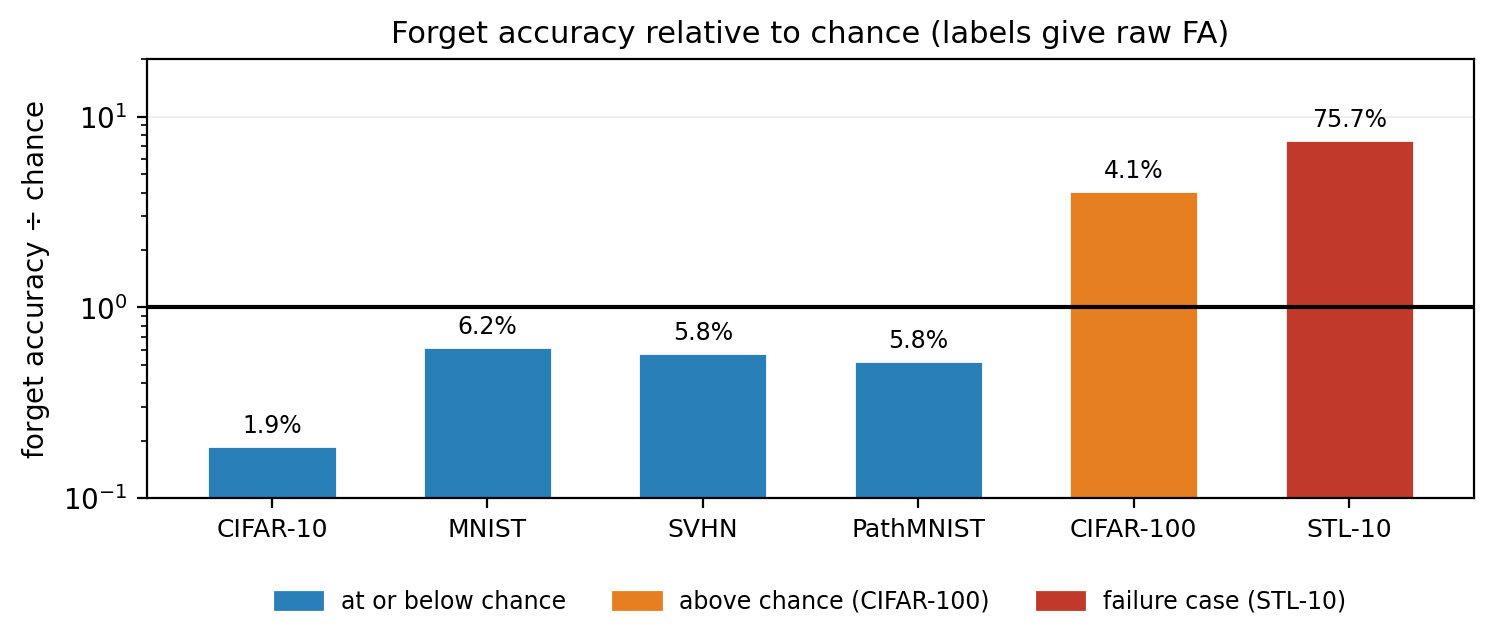
\includegraphics[width=0.86\textwidth]{fig_crossdataset.png}
\caption{\textbf{Forget accuracy relative to the chance level.} Raw forget
accuracy is not comparable across datasets: CIFAR-100's $4.1\%$ is
\emph{above} its $1\%$ chance level while MNIST's $6.2\%$ is \emph{below} its
$10\%$ one. Dividing by $100/K$ puts ``at chance'' at $1.0$ everywhere. Four
datasets sit below chance, CIFAR-100 above it despite a ${\sim}95$pp reduction,
and STL-10 above it at \rev{its 15-epoch cap, though not at 60 epochs}
(\S\ref{sec:crossdataset_stl}).}
\label{fig:crossdataset}
\end{figure}

\paragraph{The projection alone does not unlearn.}
The \emph{projection-only} row is the direct projected-gradient baseline: A-GEM
projection applied to plain gradient ascent, with the KD anchor and the
retain-confusion target removed. It preserves the retain set almost perfectly
($\mathrm{RA} = 99.90\%$), which is what the guarantee promises and all that it
promises---but it stops at $\mathrm{FA} = 18.66\%$, above the $10\%$ chance
level, and halts on the retain-loss budget rather than on the forget target.
Read together with the equal-compute ablation (Table~\ref{tab:ablation}), where
\emph{removing} the projection costs $47.4$pp of retain accuracy, this
delineates the division of labour precisely: the projection supplies retain
safety and nothing else, while the \klr{} objective is what actually drives
forget accuracy to chance. Neither component is sufficient alone, which is the
substantive content of the ablation.

\paragraph{CIFAR-100: scaling to 100 classes.}
Table~\ref{tab:cifar100} gives per-class results (base model TA~$=78.5\%$,
chance $=1\%$). \ours{} reduces FA from ${\sim}99\%$ to a mean of $4.07\%$
(median $1.60\%$) while holding RA at $92.19\%$, with MIA averaging $0.500$.
Eight of nine classes reach FA~$\le 6.8\%$; class~60 is an outlier at $17.8\%$
that does not converge within the 20-epoch budget, and it alone accounts for the
gap between the mean and the median (excluding it, mean FA is $2.35\%$). Unlike
the 10-class datasets, CIFAR-100 does not reach its $1\%$ chance level, so we
report it as a ${\sim}95$pp reduction rather than as forgetting to chance.

\begin{table}[t]
\centering
\caption{\textbf{CIFAR-100 class-level forgetting} (single seed per class,
chance $=1\%$). $^*$Class~60 does not converge within the 20-epoch budget.}
\label{tab:cifar100}
\begin{tabular}{@{}ccccc@{}}
\toprule
Forget class & TA (\%) & FA (\%)$\downarrow$ & RA (\%) & MIA \\
\midrule
10 & 77.23 & 4.20 & 92.84 & 0.485 \\
20 & 76.69 & 1.60 & 92.80 & 0.485 \\
30 & 75.18 & 1.40 & 91.03 & 0.486 \\
40 & 77.19 & 6.80 & 93.14 & 0.506 \\
50 & 76.25 & 0.60 & 92.31 & 0.562 \\
60$^*$ & 76.76 & 17.80 & 92.86 & 0.445 \\
70 & 75.38 & 1.60 & 90.89 & 0.482 \\
80 & 74.95 & 1.00 & 91.51 & 0.553 \\
90 & 75.87 & 1.60 & 92.32 & 0.498 \\
\midrule
\textbf{Mean} & \textbf{76.17} & \textbf{4.07} & \textbf{92.19} & \textbf{0.500} \\
\textbf{Median} & \textbf{76.25} & \textbf{1.60} & \textbf{92.31} & \textbf{0.486} \\
\bottomrule
\end{tabular}
\end{table}

\subsection{Momentum in Detail}\label{app:momentum}

The most direct route to an exact per-step guarantee is to remove momentum, so
that the applied update \emph{is} the projected gradient. Table~\ref{tab:momentum}
shows what that costs. With $\mu=0$ and all else fixed, \ours{} fails to forget
on five of six datasets: FA remains at $95.9\%$ on MNIST, $99.7\%$ on STL-10,
$73.7\%$ on CIFAR-100, and $61.9\%$ on SVHN. Retain accuracy stays high
throughout---but only because the model barely moves; high RA together with high
FA is the signature of a method that preserves retained knowledge by declining
to unlearn.

This is the empirical content of our central methodological claim. A per-step
guarantee stated for the momentum-free update would be exact and
implementation-matched, yet would describe a method that does not unlearn.
Projecting the post-momentum update instead keeps the guarantee exact
\emph{and} recovers forgetting on every dataset where it is attainable.

\begin{figure}[t]
\centering
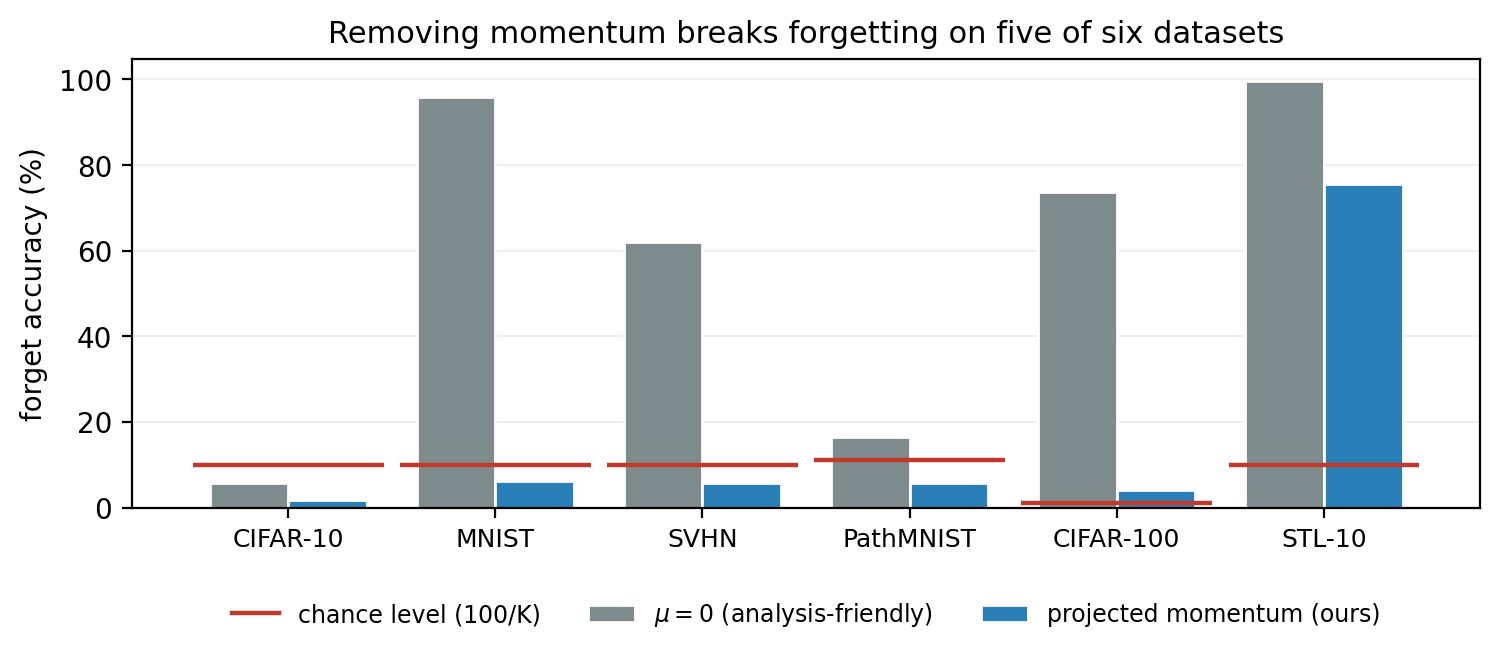
\includegraphics[width=0.86\textwidth]{fig_momentum.png}
\caption{\textbf{Momentum is not incidental.} Forget accuracy with momentum
removed ($\mu=0$, grey) against the projected-momentum update (blue), with each
dataset's chance level in red. The momentum-free configuration---the one for
which an exact guarantee is easiest to state---fails to forget on five of six
datasets. Retain accuracy stays high throughout (Table~\ref{tab:momentum}),
because the model barely moves.}
\label{fig:momentum}
\end{figure}

\paragraph{Is the dependence ours, or the field's?} A natural objection is that
this ablation only tells us something about \ours{}. If every gradient-based
unlearning rule collapses without momentum, the finding is about optimisers and
not about our design; if only ours does, the hard constraint is fragile. We
therefore repeated the ablation across four update rules on the two datasets
where Table~\ref{tab:momentum} shows the largest effect, at \emph{equal compute}
with stopping disabled so that the momentum change is not confounded with step
count (Table~\ref{tab:momentum_rules}).

\begin{table}[t]
\centering
\caption{\textbf{Where the momentum dependence comes from} (equal compute, 12
epochs on MNIST and 15 on SVHN, dual stopping disabled). $\Delta$ is the increase
in forget accuracy when momentum is removed, so larger is more dependent.
Grouping by forget objective separates the rows cleanly; grouping by whether the
projection is used does not.}
\label{tab:momentum_rules}
\begin{tabular}{@{}llcccc@{}}
\toprule
Update rule & Forget objective & Projection & MNIST $\Delta$ & SVHN $\Delta$ & mean \\
\midrule
\ours{}            & $\KL \to p_r$      & yes & $+95.3$ & $+62.4$ & $\mathbf{+78.8}$ \\
\texttt{kl\_uniform} & $\KL \to$ uniform & yes & $+84.9$ & $+56.3$ & $\mathbf{+70.6}$ \\
\addlinespace
projection only    & gradient ascent  & yes & $+16.5$ & $+13.2$ & $+14.8$ \\
gradient ascent    & gradient ascent  & no  & $+11.5$ & $+12.5$ & $+12.0$ \\
\bottomrule
\end{tabular}
\end{table}

Every rule degrades without momentum, including plain gradient ascent, which
uses no projection at all---so the dependence is not an artefact of operating
under a hard per-step constraint. But the rules do not degrade equally, and the
grouping is informative. The two KL-based objectives lose $70$--$79$pp of forget
accuracy on average, the two gradient-ascent objectives $12$--$15$pp: a factor
of $5.6$. Meanwhile the like-for-like comparison that isolates the
projection---gradient ascent with it ($+14.8$) against gradient ascent without
it ($+12.0$)---differs by only $2.8$pp.

The momentum dependence therefore belongs to the \emph{forget objective}, not to
the projection. The reason is visible in the objective itself: $\KL(p_\theta(x_f)
\| p_r)$ is bounded and its gradient vanishes as $p_\theta \to p_r$, so the
per-step signal is small and the $1/(1-\mu) = 10\times$ amplification that
momentum supplies (Lemma~\ref{lem:vel}) is what makes progress possible at
all. Gradient ascent maximises an unbounded loss and needs no such
amplification, which is also why it damages the retained model.

This sharpens rather than weakens the section's claim. The point was never that
momentum is uniquely important to \ours{}; it is that the guarantee must be
stated for the update the optimiser applies, and any method whose objective
requires momentum inherits that requirement. A momentum-free analysis is
convenient for exactly the objectives that cannot afford to be momentum-free.

\subsection{Auditing the Guarantee at Step Level}\label{sec:alignment}

We log every gradient step of a CIFAR-10 class-0 run (120 steps) and check
Theorem~\ref{thm:retain_safety} directly rather than assuming it.

\begin{itemize}
\item \textbf{The constraint is active, not vacuous.} All $120/120$ steps have
$\langle v_t,\gr\rangle < 0$, so the projection fires at every step. Projection
here is not an occasional correction: without it, every step would increase
retain loss to first order.
\item \textbf{The guarantee holds.} After projection,
$\langle u_t,\gr\rangle \ge 0$ at every step to floating-point precision. The
largest relative violation is
$\langle u_t,\gr\rangle/(\|u_t\|\|\gr\|) = -7.4\times 10^{-7}$, against a
float32 accumulation scale of ${\sim}4\times 10^{-4}$ for sums over 11.2M
parameters; the mean relative alignment is positive
($+2.2\times 10^{-8}$). The implied worst-case first-order retain increase is
$3.1\times 10^{-7}$, three orders of magnitude below the observed per-step
retain-loss fluctuation ($1.8\times 10^{-4}$). We therefore state the guarantee
as holding to float32 precision, and recommend float64 accumulation for the
inner products in reference implementations.
\item \textbf{The norm bound is respected.} $\|u_t\|$ reaches a maximum of
$9.16$ against the theoretical bound $c/(1-\mu)=10$, with mean $7.35$---close to
but never exceeding the bound, confirming both that the bound is tight and that
momentum's amplification is being realised.
\item \textbf{Retain loss is controlled.} The mean per-step change in mini-batch
retain CE is $-7.9\times 10^{-5}$ (i.e.\ decreasing), with a maximum single-step
increase of $+1.05\times 10^{-3}$, consistent with the $O(\eta^2)$ term of
Eq.~\ref{eq:thm1}.
\end{itemize}

\subsection{BatchNorm Recalibration in Detail}\label{app:bn}

Table~\ref{tab:gn} reports \ours{} with a GroupNorm backbone across datasets.
GroupNorm keeps forgetting intact on four of five datasets at a modest TA cost
(e.g.\ CIFAR-10 $84.16\%$ vs $86.13\%$), while removing the BN-recalibration
mechanism by construction, since there are no batch statistics to recalibrate.
STL-10 is under-trained under GroupNorm as it is under BN, at \rev{its epoch cap}
(\S\ref{sec:crossdataset_stl}).

\begin{table}[t]
\centering
\caption{\textbf{\ours{} with a GroupNorm backbone} (3-seed means). GroupNorm
removes the BN-recalibration vulnerability structurally. $^*$STL-10 is under-trained under
both backbones.}
\label{tab:gn}
\begin{tabular}{@{}lcccc@{}}
\toprule
\textbf{Dataset} & \textbf{TA} & \textbf{FA}$\downarrow$ & \textbf{RA} & \textbf{MIA} \\
\midrule
CIFAR-10    & 84.16 & 3.44 & 99.23 & 0.478 \\
MNIST       & 90.17 & 5.84 & 99.31 & 0.500 \\
SVHN        & 87.99 & 3.46 & 95.49 & 0.581 \\
STL-10$^*$  & 83.92 & 97.60 & 92.95 & 0.552 \\
PathMNIST   & 72.00 & 2.71 & 95.97 & 0.583 \\
\bottomrule
\end{tabular}
\end{table}

Table~\ref{tab:bnrecal} reports the diagnostic itself. The operator is
\texttt{torch.optim.swa\_utils.update\_bn} applied to the retain set: it resets
every BatchNorm buffer, sets the momentum to \texttt{None} so that PyTorch
accumulates a cumulative rather than exponential average, and runs forward
passes with no backward pass and no weight update. The resulting statistics are
therefore the exact retain-set statistics, independent of the pre-attack buffers
and idempotent in the data. We verify after every run that all learnable
parameters are bit-identical, so nothing but the buffers can have changed. Then
$\Delta F = \mathrm{post} - \mathrm{pre}$ separates weight-level forgetting
($\Delta F \approx 0$) from forgetting mediated by batch statistics
($\Delta F \gg 0$). We also report a weaker variant---forward passes in
\texttt{train} mode under the default exponential average, which is what an
earlier version of this work used---and the two agree to within $1.2$pp on every
row, and to $0.02$pp on the \ours{} row that carries the finding, so the choice
of estimator is not what drives the result. All
accuracies here are measured under deterministic (test-time) transforms; leaving
training augmentation active perturbs individual rows by several points.



\paragraph{The vulnerability is ours, not the field's---in our reproductions.}
The baseline rows matter more than \ours{}'s. Every one of them is unaffected by
recalibration---the largest movement is SCRUB's $-3.6$pp, in the direction of
\emph{more} forgetting---and so is the base model, which is the control that
matters: recalibrating a normally trained network changes nothing, because its
statistics already agree with its weights. Only \ours{} carries a mismatch.
$\Delta F = +98.4$pp means the attack does not merely degrade the unlearning but
\emph{undoes} it: forget accuracy returns to $99.7\%$ and test accuracy to
$92.9\%$\rev{---the values recalibration gives the base model itself ($99.8\%$
and $92.9\%$)}---without a single weight being modified. On a BatchNorm backbone, what \ours{} produces is not an
unlearned model but an unlearned model's statistics.

We qualify the first half of that heading deliberately. \rev{Concurrent work
\citep{kalani2026batchnorm} reports large recoveries for SalUn ($+62.1$pp) and
Bad Teacher ($+78.2$pp) under their reference implementations, where we measure
none. We ran the identical operator, so the disagreement is not in the attack
but in how the unlearned checkpoints were produced. Our implementations end
every epoch with a full pass over retained data in train mode, which recomputes
the running statistics before the checkpoint is saved; \citet{kalani2026batchnorm}
run Bad Teacher's BatchNorm in eval mode, and find that SalUn's recovery
disappears once at least a quarter of each unlearning batch is retained data.}
Our claim is therefore that the vulnerability is \ours{}-specific \emph{among
the checkpoints we trained}, not that these baselines are immune in general.

We attribute it, tentatively, to the interaction between our own design choice
and BatchNorm. \ours{} freezes the normalisation statistics during unlearning so
that class-homogeneous forget batches cannot corrupt them; the weights therefore
adapt against \emph{fixed} statistics, and the resulting decision boundary is
valid only for those statistics. Methods that let the statistics move during
unlearning never build that dependence. Freezing BatchNorm is thus necessary but
not sufficient: it prevents the statistics from manufacturing apparent
forgetting, and simultaneously makes the weights depend on them.
\added{Section~\ref{sec:bn_robust} puts this attribution to an interventional
test: keeping the statistics consistent with the weights throughout unlearning
removes the vulnerability.}

The GroupNorm backbone removes the mechanism by construction---there are no batch
statistics to recalibrate---at a cost of $2.0$pp of test accuracy
(Table~\ref{tab:gn}). The ViT-B/16 backbone
(\S\ref{sec:vit}) does the same for a different reason: LayerNorm normalises
per example at inference and keeps no running statistics either. Two
architectures with unrelated designs are both outside the operator's reach, and
both unlearn properly, which locates the defect in the normalisation scheme
rather than in gradient projection.

We state the limit of that plainly: neither backbone \emph{resists} the attack,
because the attack is undefined on them. This is a design change, not
demonstrated robustness, and a method that must avoid BatchNorm to be safe is
constrained in a way the guarantee itself does not capture. What the two rows do
establish is that the defect is separable from \ours{}'s mechanism---it is a
property of freezing statistics that a normalisation layer keeps, and it
disappears wherever there are no such statistics. \added{The next subsection
removes the constraint itself: it keeps BatchNorm, and makes \ours{} robust to
the attack rather than outside its reach.}

\begingroup\color{revised}% ---- new subsection: everything to \endgroup is added
\subsection{BN-robust \ours{} in Detail}\label{app:bn_robust}

The diagnosis above points at its own remedy: if the weights learn to forget
against statistics that are allowed to go stale, the statistics should never be
stale. BN-robust \ours{} makes three changes to Algorithm~\ref{alg:excise}
(Figure~\ref{fig:bnrobust_mech}). It leaves the update rule untouched, \rev{so
Theorem~\ref{thm:retain_safety} holds at every step for the retain objective
under the statistics in force during that step; the recalibration between steps
is not covered by it}.
\begin{enumerate}
\item \emph{Track the weights.} Before every step the BatchNorm statistics are
recomputed, $\phi \leftarrow R(\theta, B_r)$, with the attacker's own operator
$R$ (\texttt{update\_bn}) on a fresh sample $B_r$ of $512$ retain images. The
step's forward and backward passes then run under statistics consistent with the
current weights. Forget batches still never touch the statistics: this keeps
the half of freezing that was right and drops the half that was wrong.
\item \emph{Ship consistent statistics.} After the last step,
$\phi \leftarrow R(\theta_T, \Dr)$ on the whole retain set under test-time
transforms---exactly what the attacker computes.
\item \emph{Stop on the forget accuracy that ships.} The stopping rule of
\S\ref{sec:stopping} reads FA under $R(\theta, \Dr)$ with test-time transforms,
not under the in-loop statistics. If the target is not met within the epoch
budget, the epoch with the lowest such FA inside the retain budget is shipped
instead of the last one.
\end{enumerate}
\begin{figure}[t]
\centering\color{revised}
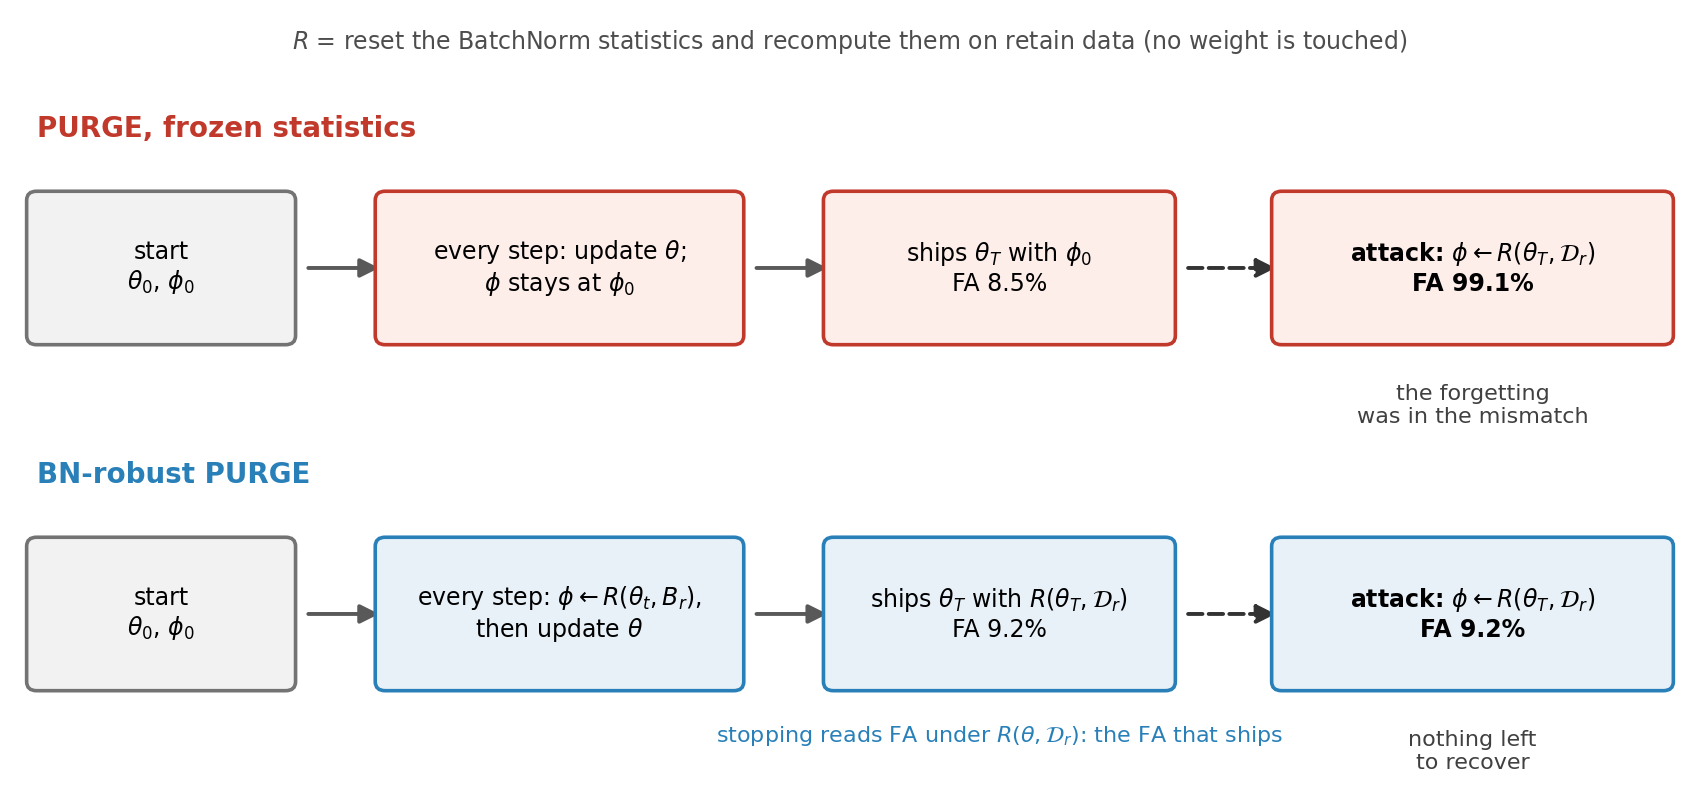
\includegraphics[width=\textwidth]{fig_bnrobust_mechanism.png}
\caption{\added{\textbf{What BN-robust \ours{} changes.} $R$ resets the BatchNorm
statistics and recomputes them on retain data without touching a weight. With
frozen statistics the forgetting lives in the mismatch between $\theta_T$ and
$\phi_0$, and the attack removes it; BN-robust ships statistics consistent with
its weights, so the attack has nothing to recover. Forget accuracies are
CIFAR-10 class~0, means over three seeds (Table~\ref{tab:bnrobust}).}}
\label{fig:bnrobust_mech}
\end{figure}

Because $R$ is idempotent, change~2 makes the attack a no-op on the shipped model
by construction, so $\Delta F = 0$ is not by itself evidence here. The question
this variant must answer is whether FA is still low once $\phi$ cannot be
stale. Two of the tests below are not no-ops by construction: the
exponential-average operator, and recalibration on data other than the retain
set.

Change~3 is not cosmetic. Without it, the FA that triggers stopping is read under
the in-loop statistics---a few hundred augmented images, one step behind---on
augmented forget images. On CIFAR-10 that reading falls short of the shipped FA
by between $-1.0$ and $+9.0$pp depending on the class, and runs stopped at
``FA $\le 10\%$'' shipped at $7.2$--$16.7\%$ (Figure~\ref{fig:bnrobust_stop}). With change~3 the shipped FA meets
the target, and the seed-to-seed spread on class~0 falls from $1.90$ to
$0.08$pp (Table~\ref{tab:bnrobust}). The stopping check need not use the whole
retain set. Computing it on $10{,}240$ images reproduced every stopping decision
of the full check on all three seeds and cut wall-clock by $16\%$; the shipped
statistics still use the full set.

\begin{figure}[t]
\centering\color{revised}
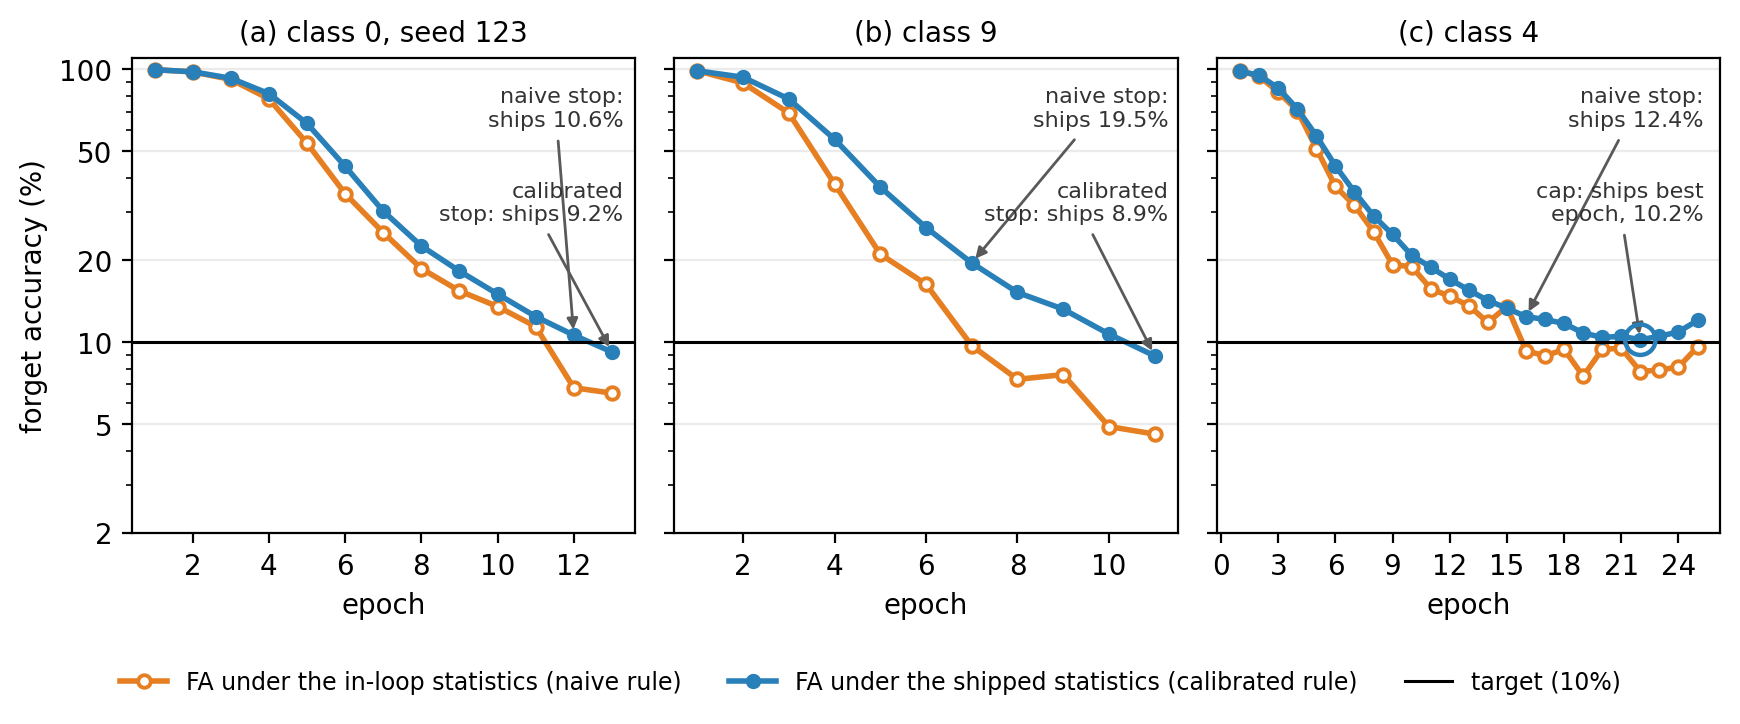
\includegraphics[width=\textwidth]{fig_bnrobust_stopping.png}
\caption{\added{\textbf{Why stopping must be calibrated.} Forget accuracy per epoch
under the in-loop statistics (what naive stopping reads) and under the
statistics that ship (what calibrated stopping reads); log scale. The in-loop
reading runs below the shipped one, so a naive rule stops early and ships above
chance: (a)~one epoch early on class~0, (b)~four epochs early on class~9,
shipping $19.5\%$ instead of $8.9\%$. (c)~On class~4 the shipped FA plateaus just
above $10\%$ and the run reaches the epoch cap; the best-epoch rule ships epoch~22
($10.2\%$) rather than the last ($12.0\%$).}}
\label{fig:bnrobust_stop}
\end{figure}

These experiments were run after the checkpoints behind
Table~\ref{tab:bnrecal} became unavailable. They use an earlier CIFAR-10 base
(test accuracy $93.97\%$, against $95.5\%$ there), a GroupNorm base retrained for
$100$ rather than $200$ epochs ($91.89\%$), and a retrained MNIST base
($99.59\%$). Their absolute numbers are therefore not comparable row for row
with the rest of \S\ref{sec:experiments}; every comparison below is between arms
that share a base.



\paragraph{It survives the attack it was built against, and two it was not.}
Calibrated BN-robust forgets class~0 to $9.19\%$ and stays at $9.18\%$ under
recalibration (Figure~\ref{fig:bnrobust_attack}a), while the frozen configuration
returns to $99.12\%$ with test accuracy back at $94.1\%$---the original model. The exponential-average
operator, which is not idempotent and therefore not a no-op here, moves
BN-robust by at most $+0.3$pp. Nor does robustness depend on the attacker using
the retain set. On the naive-stopping checkpoints, recomputing the statistics
on the full training set, forget class included, or on the test set---data
BN-robust never trained under---moves its FA by $-1.0$ to $-1.2$pp, towards more
forgetting, while the frozen configuration still recovers to $97.4\%$ and
$97.3\%$ (Figure~\ref{fig:bnrobust_attack}b).

\paragraph{Every class, and a second dataset.}
On all ten CIFAR-10 classes (seed~$42$; Table~\ref{tab:app_bnrobust} and
Figure~\ref{fig:app_bnrobust}), the
frozen configuration recovers to $94.7$--$99.3\%$ under the attack, while
BN-robust's FA moves by at most $0.06$pp under either stopping rule. With
calibrated stopping every class ships between $6.7\%$ and $10.2\%$, inside three
standard errors of chance ($11.3\%$ for $5{,}000$ images); with naive stopping,
five of the ten did not. One class needed the fallback. Class~4 hovered at
$10.2$--$10.9\%$ for six epochs without crossing $10\%$ and reached the epoch
cap, and the rule shipped its best epoch ($10.2\%$) rather than the last
($11.9\%$, with retain accuracy $1.4$pp lower). On MNIST, over three seeds, the
frozen configuration's forgetting is undone completely ($0.00\% \to 99.97\%$,
with test accuracy back to $99.56\%$ against the base's $99.59\%$), and
BN-robust holds ($3.78\% \to 3.87\%$, test accuracy $90.10\%$).

\paragraph{What it costs, and why it is slower.}
Against the frozen configuration, BN-robust gives up $1.8$pp of retain accuracy
and $0.9$pp of test accuracy and takes about seven times the wall-clock, most of
it because it needs $13$ epochs instead of $2$. We read the slower forgetting as
the substance rather than the overhead. The frozen configuration reaches its
target in two epochs largely through the statistics mismatch, which the attack
shows is not forgetting at all; once the statistics track the weights, the
forgetting has to happen in the weights. BN-robust's test accuracy, $84.30\%$,
is close to the $84.6\%$ expected from removing one class of ten from a
$93.97\%$ model. Against GroupNorm, BN-robust keeps $1.2$pp more test accuracy,
mostly because it can start from the stronger BatchNorm base, and it needs
neither a change of architecture nor a retrained base model.
Membership-inference AUROC stays between $0.48$ and $0.52$ for every unlearned
row.

\paragraph{What it does and does not establish.}
Unlike GroupNorm or a transformer, this is robustness rather than immunity by
construction: the attack is defined on the model, runs, and finds nothing to
recover. It is robustness to one attack, though. BN-robust changes only how the
normalisation statistics are maintained, so it does nothing against attacks that
modify the weights, such as fine-tuning recovery (\S\ref{sec:limitations}), and
we have tested it on two datasets rather than six. Within that scope, \ours{} no
longer has to choose between BatchNorm and its forgetting: BN-robust \ours{},
\ours{} with GroupNorm, and \ours{} on a transformer are all configurations we
would deploy.
\endgroup% ---- end of the added subsection

\subsection{A Transformer Backbone}\label{sec:vit}

Every result so far uses ResNet-18, so the projection has only ever been applied
to a convolutional network. We repeat CIFAR-10 class~0 on ViT-B/16 under the
identical algorithm, with representation erasure disabled as everywhere else,
over three seeds.

\begin{table}[t]
\centering
\caption{\textbf{ViT-B/16 against ResNet-18}, same algorithm and forget targets
as Table~\ref{tab:cross}\rev{; the ViT runs check forget accuracy every step.
Chance is $10\%$ on CIFAR-10 and $1\%$ on CIFAR-100. The projection fires on
$98$--$100\%$ of steps, as it does on ResNet-18.}}
\label{tab:vit}
\begin{tabular}{@{}lcccc@{}}
\toprule
Backbone & TA & FA$\downarrow$ & RA & MIA \\
\midrule
\multicolumn{5}{@{}l}{\rev{\emph{CIFAR-10, class~0, three seeds}}} \\
ResNet-18 (Table~\ref{tab:cross}) & $86.13 \pm 0.02$ & $1.87 \pm 0.25$ & $100.00 \pm 0.00$ & $0.529$ \\
ViT-B/16                          & $87.05 \pm \rev{0.09}$ & $9.71 \pm \rev{0.27}$ & $\phantom{0}97.55 \pm \rev{0.10}$ & $0.453$ \\
\midrule
\multicolumn{5}{@{}l}{\rev{\emph{CIFAR-100, classes $10,\dots,90$, one seed each, 20-epoch cap}}} \\
\rev{ResNet-18 (Table~\ref{tab:cross})} & \rev{$76.17 \pm 0.86$} & \rev{$4.07 \pm 5.51$} & \rev{$92.19 \pm 0.84$} & \rev{$0.500$} \\
\rev{ViT-B/16} & \rev{$81.97 \pm 0.66$} & \rev{$24.00 \pm 23.16$} & \rev{$91.86 \pm 0.73$} & \rev{$0.435$} \\
\bottomrule
\end{tabular}
\end{table}

\rev{On CIFAR-10} forgetting transfers: FA reaches $9.71\%$, below the $10\%$
chance level, with retain accuracy at $97.55\%$ and test accuracy slightly
\emph{above} the ResNet-18 result. The gap in FA against ResNet-18's $1.87\%$ is not a weaker
result but a different stopping point---both runs use $\tau_F = 10\%$, and
the ViT run halts as soon as it crosses that threshold (epoch~3, mid-epoch),
whereas the ResNet-18 run overshoots it. \S\ref{sec:experiments} shows that
overshoot is an artifact of check granularity rather than a property of either
backbone.

\rev{On CIFAR-100 it does not transfer within the same 20-epoch cap. On the nine
classes of Table~\ref{tab:cross}, ViT-B/16 ends with FA between $4.0\%$ and
$82.0\%$ (mean $24.0\%$) against a $1\%$ chance level, so no class reaches
chance, where ResNet-18 ends at $4.07\%$ and reaches chance at 60 epochs.
Retain accuracy ($91.9\%$) matches ResNet-18's. We have not tested whether a
longer budget closes the gap, as it does for ResNet-18; until then the
transformer result holds for CIFAR-10 only.}

Two things follow. First, the conflict the projection resolves is not an artifact
of convolutional architectures: the projection fires on $99$--$100\%$ of steps
here as well, so forget and retain gradients oppose one another just as
routinely in a transformer. Second, and more usefully,
ViT normalises with LayerNorm, which computes statistics per example at
inference and stores none. It is therefore outside the reach of the
recalibration operator of \S\ref{sec:bn_results} for the same structural reason
as GroupNorm, but by way of a completely different architecture---which is what
makes the pair informative rather than merely repetitive.

\subsection{Component Ablation}\label{sec:ablation}

A component ablation run in the deployed configuration is uninformative here,
and the reason is instructive. Under the projected-momentum optimiser every
variant reaches the forget-accuracy target inside the first check interval, so
dual stopping halts them all after one epoch and each looks equally good: in the
upper half of Table~\ref{tab:ablation}, removing the projection costs
$0.09$pp of retain accuracy. That number is an artefact of stopping, not a
measurement of what the projection does.

We therefore also run every variant at \emph{equal compute}, with stopping
disabled throughout (lower half). The picture inverts.

\begin{table}[t]
\centering
\caption{\textbf{Component ablation} (CIFAR-10 class~0, seed 42). Upper: the
deployed configuration, where dual stopping halts every variant after one epoch.
Lower: equal compute, 15 epochs, stopping disabled for all variants---the same
comparison without the stopping confound. \texttt{+rep} and \texttt{+gate}
re-introduce the two components removed in \S\ref{sec:method}.}
\label{tab:ablation}
\begin{tabular}{@{}llcccc@{}}
\toprule
& Variant & TA & FA & RA & MIA \\
\midrule
\multirow{7}{*}{\rotatebox{90}{\emph{stopping on}}}
 & full \ours{}      & $86.10$ & $2.14$ & $100.00$ & $0.528$ \\
 & $-$KD             & $85.56$ & $0.80$ & $99.99$  & $0.516$ \\
 & $-$projection     & $84.87$ & $0.78$ & $99.91$  & $0.513$ \\
 & selective-layer   & $86.26$ & $3.26$ & $100.00$ & $0.528$ \\
 & $+$rep            & $86.10$ & $2.14$ & $100.00$ & $0.528$ \\
 & $+$gate           & $86.10$ & $2.14$ & $100.00$ & $0.528$ \\
 & $-$stopping       & $85.71$ & $0.00$ & $99.98$  & $0.472$ \\
\midrule
\multirow{6}{*}{\rotatebox{90}{\emph{equal compute}}}
 & full \ours{}      & $85.70$ & $0.00$ & $99.98$  & $0.472$ \\
 & $-$KD             & $85.66$ & $0.00$ & $99.94$  & $0.475$ \\
 & $-$projection     & $\mathbf{44.37}$ & $0.00$ & $\mathbf{52.55}$ & $0.436$ \\
 & selective-layer   & $85.76$ & $0.00$ & $99.99$  & $0.469$ \\
 & $+$rep            & $85.74$ & $0.00$ & $99.98$  & $0.473$ \\
 & $+$gate           & $87.16$ & $19.28$ & $100.00$ & $0.539$ \\
\bottomrule
\end{tabular}
\end{table}

\paragraph{The projection is what makes unlearning survivable.}
At equal compute, removing it costs $41.3$pp of test accuracy and
$47.4$pp of retain accuracy: the model collapses to $44.4/52.6$ against
$85.7/99.98$ for the full method. This is the empirical counterpart of
Theorem~\ref{thm:retain_safety}, and it is a far larger effect than the
stopping-confounded comparison suggests. Note also that the two rows disagree
about the \emph{sign} of the conclusion---one reports the projection as
costless, the other as indispensable---which is why we report both rather than
whichever is more favourable.

\paragraph{KD contributes little once compute is equalised.}
Removing the distillation anchor changes retain accuracy by $0.04$pp at equal
compute. We previously attributed several points of retain accuracy to it; that
is not supported here, and we no longer claim it.

\paragraph{The removed components stay removed.}
Re-introducing representation erasure reproduces the full method to within
$0.04$pp on every metric, and re-introducing the entropy gate leaves forget
accuracy at $19.3\%$---above the $10\%$ chance level, i.e.\ it prevents the
method from forgetting. Both were dropped in \S\ref{sec:method} on the strength
of an ablation run under the previous implementation; this re-run confirms the
decision under the current one.

\subsection{How Hard Must the Constraint Be?}\label{sec:strength}

Theorem~\ref{thm:separation}(iv) argues that a soft conflict penalty biases the
update without excluding retain-harming steps, and that only a hard constraint
makes them unreachable. That is an argument about feasible sets; here we measure
what it costs in practice. We interpolate the projection with a strength
parameter $s$: at each conflicting step the update becomes
$u_t = v_t - s\,\frac{\langle v_t,\gr\rangle}{\|\gr\|^2}\gr$, so
\begin{equation}\label{eq:strength}
\langle u_t, \gr\rangle \;=\; (1-s)\,\langle v_t, \gr\rangle .
\end{equation}
At $s=0$ nothing is corrected; at $s=1$ this is \ours{}. Every intermediate
value is a soft penalty---it shrinks the conflicting component without removing
it---and by Eq.~\ref{eq:strength} it leaves $\langle u_t,\gr\rangle<0$ whenever
the raw update conflicts. All other settings are held fixed, and stopping is
disabled so that every variant sees the same compute.

\begin{table}[t]
\centering
\caption{\textbf{Projection strength} (CIFAR-10 class~0, equal compute, stopping
disabled). $s=0$ applies no correction, $s=1$ is the full hard constraint.
Forget accuracy is $0.0\%$ throughout, so the runs differ only in collateral
damage.}
\label{tab:strength}
\begin{tabular}{@{}lccccc@{}}
\toprule
$s$ & residual conflict & TA & FA & RA & MIA \\
\midrule
$0.00$ & $1.00\,\langle v_t,\gr\rangle$ & $44.35$ & $0.0$ & $52.54$ & $0.436$ \\
$0.25$ & $0.75\,\langle v_t,\gr\rangle$ & $67.84$ & $0.0$ & $81.35$ & $0.497$ \\
$0.50$ & $0.50\,\langle v_t,\gr\rangle$ & $78.03$ & $0.0$ & $92.75$ & $0.510$ \\
$0.75$ & $0.25\,\langle v_t,\gr\rangle$ & $82.99$ & $0.0$ & $98.24$ & $0.509$ \\
$1.00$ & $\mathbf{0}$ & $\mathbf{85.71}$ & $0.0$ & $\mathbf{99.98}$ & $0.472$ \\
\bottomrule
\end{tabular}
\end{table}

\begin{figure}[t]
\centering
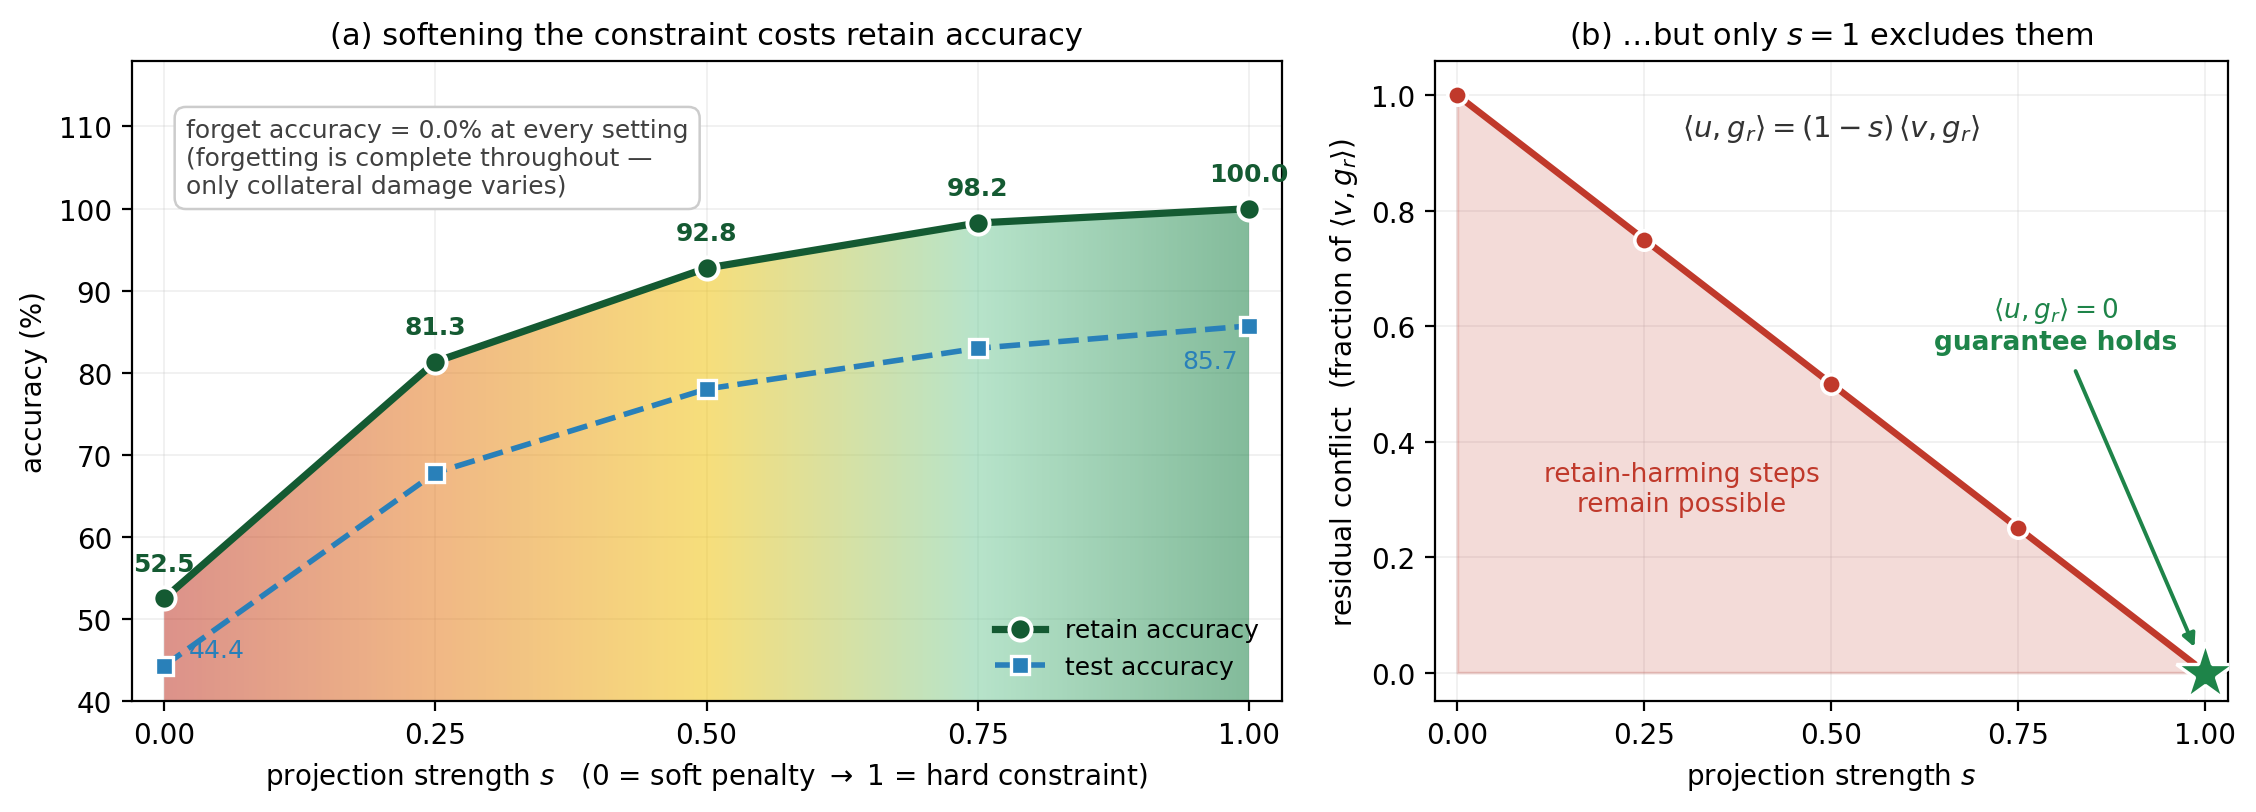
\includegraphics[width=\textwidth]{fig_strength.png}
\caption{\textbf{Hardening the constraint recovers retain accuracy
continuously, but only the endpoint carries the guarantee.}
\textbf{(a)}~Retain and test accuracy against projection strength; forget
accuracy is $0.0\%$ at every setting, so the runs differ only in collateral
damage. \textbf{(b)}~Residual conflict $(1-s)$: retain-harming steps remain
reachable for every $s<1$ and are excluded only at $s=1$. The empirical
difference between $s=0.75$ and $s=1$ is $1.7$pp of retain accuracy; the
difference in what can be proved is categorical.}
\label{fig:strength}
\end{figure}

\paragraph{Softening is expensive, and monotonically so.}
Retain accuracy falls from $99.98\%$ at $s=1$ to $52.54\%$ at $s=0$, and test
accuracy from $85.71\%$ to $44.35\%$, monotonically in between. Because forget
accuracy is $0.0\%$ at every setting, this is not a privacy--utility trade-off:
all five runs forget equally, and they differ only in how much of the retained
model they destroy on the way. The $s=0$ row reproduces the equal-compute
$-$projection ablation of Table~\ref{tab:ablation} from an independent
direction.

\paragraph{The curve is gradual, which we take as a limitation of the empirical
argument.} Most of the benefit arrives early---$s=0.25$ already recovers
$28.8$pp of retain accuracy, while the final quarter, $s=0.75\to1$, is worth
$1.7$pp. A soft penalty tuned near $s=0.75$ therefore performs almost as well as
the hard constraint on these metrics, and we do not claim otherwise. What it
does not do is satisfy Eq.~\ref{eq:strength} with equality: at $s=0.75$ a
quarter of every conflict survives into the applied update, so
$\langle u_t,\gr\rangle<0$ on conflicting steps and no per-step statement can be
made. The case for $s=1$ is therefore not that the last $1.7$pp is large, but
that it is the only setting about which anything can be proved---which is the
whole content of Theorem~\ref{thm:retain_safety}.

\paragraph{Relation to soft conflict-resolution methods.}
This is a controlled test of the mechanism that separates \ours{} from the
closest prior work \citep{patel2025learning}, not a comparison with that method:
it varies our own projection rather than reimplementing theirs, and their
penalty acts on the objective rather than on the update. What it establishes is
the general shape of the trade---that discouraging conflict helps in proportion
to how much of it is removed, and that removing all of it is what converts an
empirical tendency into a guarantee. A like-for-like comparison remains future
work (\S\ref{sec:limitations}).

\subsection{Privacy--Utility Frontier and Robustness Diagnostics}\label{sec:sweeps}

We sweep the two tolerances of Eq.~\ref{eq:problem} independently on CIFAR-10
class~0 (Table~\ref{tab:sweeps}). The results are asymmetric: one tolerance is
inert because the projection has already done its work, while the other is
genuinely active but was hidden by how coarsely we measured it.

\begin{table}[t]
\centering
\caption{\textbf{Tolerance sweeps} (CIFAR-10 class~0). Sweep~A varies the
retain-loss budget $\alpha$ at fixed $\tau_F = 10\%$; Sweeps~B and B$'$ vary
the forget-accuracy target $\tau_F$ at fixed $\alpha = 5$, checking forget
accuracy every 50 batches and every step respectively. $\alpha$ is inert. So is
$\tau_F$ under the coarse check---but only because forget accuracy crosses
the whole range between two consecutive checks; measured per step, it tracks the
requested tolerance across a $29$pp range.}
\label{tab:sweeps}
\begin{tabular}{@{}lccccc@{}}
\toprule
\multicolumn{2}{@{}l}{Sweep A: $\alpha$} & TA & FA & RA & MIA \\
\midrule
& $1.5$    & $86.10$ & $1.88$ & $100.00$ & $0.530$ \\
& $2$      & $86.10$ & $1.88$ & $100.00$ & $0.530$ \\
& $3$      & $86.10$ & $1.88$ & $100.00$ & $0.530$ \\
& $5$      & $86.10$ & $1.88$ & $100.00$ & $0.530$ \\
& $10$     & $86.10$ & $1.88$ & $100.00$ & $0.530$ \\
& $9999$   & $86.10$ & $1.88$ & $100.00$ & $0.530$ \\
\midrule
\multicolumn{2}{@{}l}{Sweep B: $\tau_F$, check every 50 batches} & TA & FA & RA & MIA \\
\midrule
& $1\%$    & $85.75$ & $\phantom{0}0.28$ & $100.00$ & $0.521$ \\
& $5\%$    & $86.10$ & $\phantom{0}1.88$ & $100.00$ & $0.530$ \\
& $10\%$   & $86.10$ & $\phantom{0}1.88$ & $100.00$ & $0.530$ \\
& $20\%$   & $86.10$ & $\phantom{0}1.88$ & $100.00$ & $0.530$ \\
& $30\%$   & $86.10$ & $\phantom{0}1.88$ & $100.00$ & $0.530$ \\
\midrule
\multicolumn{2}{@{}l}{Sweep B$'$: $\tau_F$, check every step} & TA & FA & RA & MIA \\
\midrule
& $1\%$    & $85.95$ & $\phantom{0}\mathbf{0.60}$ & $100.00$ & $0.531$ \\
& $5\%$    & $86.34$ & $\phantom{0}\mathbf{3.86}$ & $100.00$ & $0.528$ \\
& $10\%$   & $86.59$ & $\phantom{0}\mathbf{8.24}$ & $100.00$ & $0.522$ \\
& $20\%$   & $87.22$ & $\mathbf{16.24}$ & $100.00$ & $0.518$ \\
& $30\%$   & $88.10$ & $\mathbf{29.60}$ & $100.00$ & $0.515$ \\
\bottomrule
\end{tabular}
\end{table}

\paragraph{The retain budget is non-binding.}
Varying $\alpha$ over four orders of magnitude changes nothing: the retain-loss
constraint is never the active one, because the projection already prevents the
retain loss from rising. This is consistent with Theorem~\ref{thm:retain_safety}
and means $\alpha$ can be left at its default.

\paragraph{The forget target is a usable knob, but only if it is measured
finely enough.} Sweep~B contains no frontier: every target from $5\%$ to $30\%$
yields the identical operating point, $\mathrm{FA} = 1.88\%$. We previously read
this as evidence that $\tau_F$ is not a knob at all. That reading was wrong,
and Sweep~B$'$ shows why: the sweep was limited by the \emph{measurement}, not
by the method.

Forget accuracy is checked every 50 batches, and under this optimiser it falls
from ${\sim}99\%$ to below $2\%$ inside a single such interval, so every target
in between is passed unobserved and the run halts at whichever point the next
check happens to catch. Sweep~B$'$ repeats the sweep with the check evaluated at
every step---on a subsample of $\Df$, with any trigger confirmed on the full
forget set before stopping---and the frontier appears: forget accuracy tracks
the requested tolerance monotonically from $0.60\%$ to $29.60\%$, a $29$pp
range, with test accuracy rising from $85.95\%$ to $88.10\%$ as the tolerance is
relaxed and retain accuracy pinned at $100.00\%$ throughout. At
$\tau_F = 30\%$ the coarse check lands at $\mathrm{FA} = 1.88\%$ where
$29.60\%$ was reachable: a $27.5$pp overshoot attributable entirely to
measurement granularity.

Step-level traces confirm that nothing about the collapse forbids resolving it.
The largest single-step change in forget accuracy is $11.7$--$11.9$pp across
the five targets---the runs follow one trajectory and differ only in where they
leave it. A $12$pp-per-step descent is comfortably resolvable at
per-step granularity; it was invisible at 50-batch granularity. We therefore
restore the $\tau_F$ entry in Table~\ref{tab:properties}, with the
qualification that the tolerance is honoured only when the stopping rule is
evaluated at a resolution finer than the descent it is meant to catch. The cost
is one forward pass over a $512$-sample subsample per step.

\paragraph{MIA in isolation is uninformative.}
An early sign of this: the \emph{pre-unlearning} base model already attains MIA
AUROC $=0.533$ at FA~$=99.7\%$. For well-generalising classifiers, per-sample
membership carries little signal at the class level, so MIA AUROC alone cannot
certify class-level unlearning and must be paired with FA. \S\ref{sec:mia}
develops this into a sharper statement: under the standard protocol the attack
scores \emph{higher} against a model that never saw the data than against one
that memorised it.

\subsection{Distance to a Retrained Model}\label{sec:distance}

Forget accuracy asks whether the forget class is still predicted. It does not
ask whether the unlearned model \emph{behaves like} one trained without that
class, which is what unlearning is for. We therefore retrain a CIFAR-10
reference from scratch on the retain set only, keeping all $K$ output heads so
that output distributions remain comparable, and measure how far each unlearned
model sits from it (Table~\ref{tab:distance}). Two spaces are measured: the
output distribution on forget-class inputs (Jensen--Shannon divergence, and
top-1 agreement with the reference's predictions), and the penultimate feature
distribution (Fr\'echet distance).

\begin{table}[t]
\centering
\caption{\textbf{Distance to a retrained CIFAR-10 reference} (class~0). The
reference is trained on the retain set only. JS and agreement compare output
distributions on forget-class inputs; Fr\'echet compares penultimate features.
Best per column in bold. Parameter distance is reported for completeness only
(see text).}
\label{tab:distance}
\begin{tabular}{@{}lccccccc@{}}
\toprule
Method & JS$\downarrow$ & agree \%$\uparrow$ & Fr\'echet$\downarrow$ &
$\|\Delta\theta\|_2$ & FA & RA & $|\mathrm{MIA}{-}0.5|\downarrow$ \\
\midrule
SalUn        & $\mathbf{0.220}$ & $\mathbf{56.5}$ & $495.3$ & $80.6$ & $0.00$  & $97.70$ & $0.075$ \\
Bad Teacher  & $0.263$ & $47.1$ & $153.0$ & $89.7$ & $24.36$ & $89.46$ & $\mathbf{0.029}$ \\
SCRUB        & $0.562$ & $\phantom{0}8.7$ & $165.9$ & $56.6$ & $89.28$ & $97.83$ & $0.030$ \\
\midrule
\ours{}      & $0.273$ & $35.2$ & $\mathbf{13.0}$ & $43.2$ & $\phantom{0}1.76$ & $\mathbf{100.00}$ & $0.030$ \\
\bottomrule
\end{tabular}
\end{table}

\paragraph{The two spaces disagree, and no method dominates.}
\ours{} is closest to the reference in feature space by a wide margin---a
Fr\'echet distance of $13.0$ against $153$--$495$ for the baselines, a factor of
$38$ against SalUn---and it is the only method that leaves retain accuracy
untouched. SalUn is closest in output space, with the lowest JS divergence
($0.220$ against our $0.273$) and the highest agreement with the reference's
predictions on forget inputs ($56.5\%$ against our $35.2\%$). We report this
plainly: on the metric that most directly operationalises ``behaves like a
retrained model'' on forget inputs, \ours{} is second.

The disagreement is itself the finding. A method can route forget-class inputs
much as a retrained model would while carrying internal representations far from
it, or preserve those representations while routing inputs differently. Reporting
a single distance would have concealed this, and which number one reports would
have determined which method appeared better. We therefore recommend that
distance-to-retrained be reported in both spaces, and we do so.

\paragraph{SCRUB is far away because it has not unlearned.}
Its JS divergence is more than twice ours and its agreement with the reference
is $8.7\%$, but this follows from $\mathrm{FA} = 89.3\%$: a model that still
classifies the forget class correctly cannot resemble one that never saw it.
This is a useful sanity check on the metric---it ranks non-unlearning last---%
rather than a criticism of SCRUB under a different operating point.

\paragraph{Parameter distance is uninformative.}
$\|\Delta\theta\|_2$ orders the methods differently again ($43.2$ for \ours{},
$56.6$ for SCRUB, $80.6$ for SalUn, $89.7$ for Bad Teacher) and tracks neither
behavioural measure. Permutation and scaling symmetries mean two functionally
identical networks can sit far apart in parameter space, so we report it for
completeness and draw no conclusion from it.

\subsection{Membership Inference, Recalibrated}\label{sec:mia}

Every MIA number reported so far, in this paper and in much of the unlearning
literature, is read against a target of $0.5$: the attack should be unable to
distinguish forget-class training samples from forget-class test samples. We ran
four attacks against a retrained reference to check that target, and it does not
survive.

We evaluate four threshold-free signals---negative loss, maximum confidence,
negative entropy, and modified entropy \citep{song2021systematic}, the last of
which uses the true label and so separates confidently-correct from
confidently-wrong predictions---and report AUROC together with true-positive
rate at $1\%$ false-positive rate. The second matters because an attack that
identifies a few members with near-certainty is a real privacy failure that an
average AUROC of $0.5$ can conceal.

\begin{table}[t]
\centering
\caption{\textbf{MIA suite on CIFAR-10 (class~0).} Members are forget-class
training samples, non-members forget-class test samples ($5000$ vs $1000$). The
retrained reference trained on \emph{neither} group, so it is the empirical
target; the base model trained on the members and is the opposite anchor.
TPR is at $1\%$ FPR.}
\label{tab:mia}
\begin{tabular}{@{}lcccccccc@{}}
\toprule
& & \multicolumn{2}{c}{loss} & \multicolumn{2}{c}{mentr} &
\multicolumn{2}{c}{conf} & entropy \\
\cmidrule(lr){3-4}\cmidrule(lr){5-6}\cmidrule(lr){7-8}\cmidrule(lr){9-9}
Model & FA & AUROC & TPR & AUROC & TPR & AUROC & TPR & AUROC \\
\midrule
retrained (reference) & $0.0$  & $0.694$ & $12.5\%$ & $0.646$ & $9.9\%$ & $0.435$ & $0.1\%$ & $0.422$ \\
base (no unlearning)  & $100.0$ & $0.483$ & $0.0\%$  & $0.486$ & $0.0\%$ & $0.482$ & $0.0\%$ & $0.479$ \\
\midrule
SalUn                 & $0.0$   & $0.500$ & $0.0\%$  & $0.537$ & $2.3\%$ & $0.463$ & $0.0\%$ & $0.461$ \\
Bad Teacher           & $24.8$  & $0.485$ & $0.2\%$  & $0.493$ & $0.2\%$ & $0.455$ & $0.6\%$ & $0.444$ \\
SCRUB                 & $89.5$  & $0.477$ & $0.4\%$  & $0.478$ & $0.4\%$ & $0.467$ & $0.4\%$ & $0.462$ \\
\ours{}               & $2.0$   & $0.693$ & $1.4\%$  & $0.691$ & $1.3\%$ & $0.369$ & $0.0\%$ & $0.340$ \\
\bottomrule
\end{tabular}
\end{table}

\paragraph{The retrained reference does not score $0.5$.}
It scores $0.694$ on the loss attack, with a true-positive rate of $12.5\%$ at
$1\%$ false positives. This model trained on \emph{neither} group: to it, forget
train and forget test are both non-members. The attack is therefore not
detecting membership. It is detecting that the CIFAR-10 train and test splits of
class~0 differ in difficulty, and that difference is visible through any model
that has not memorised either. A target of $0.5$ is wrong for this protocol, and
$0.694$ is the level a perfectly unlearned model actually exhibits.

\paragraph{The attack works \emph{better} against the model that never saw the
data.} The base model memorised all $5000$ members and classifies them at
$100\%$; the standard intuition says it should be the most attackable thing in
the table. It scores $0.483$---below chance, and $0.21$ below the retrained
reference. A well-generalising classifier treats members and non-members of a
class alike, leaving no signal, whereas a model that never saw the class makes
errors whose pattern differs between the splits. Under this protocol, MIA AUROC
is anti-correlated with memorisation.

\paragraph{The choice of target reverses the ranking.}
Read against $0.5$, \ours{} looks like the \emph{worst} method in the table
($|{\rm AUROC}-0.5| = 0.193$) and SalUn like the best ($0.000$). Read against the
retrained reference---the model unlearning is supposed to imitate---the order
inverts: \ours{} is nearest ($|{\rm AUROC}-{\rm ref}| = 0.001$) and SalUn is
$0.194$ away. We report both columns rather than the flattering one, and we note
that our own earlier claim of ``MIA within $0.035$ of the ideal $0.5$'' was
resting on the wrong reference point.

We do not want to over-read the agreement between \ours{} and the reference. It
is one dataset, one forgotten class, one protocol, and matching to $0.001$ is
closer than the measurement warrants; what the data supports is that \ours{}
sits near the retrained model on this attack while the baselines sit near $0.5$,
not that it matches it exactly.

\paragraph{On a second dataset the reference is not even a \emph{constant}.}
The argument above rests on one dataset and one class, which is thin for a claim
about everyone's protocol, so we repeated it on PathMNIST, retraining a
reference for each of four classes (Table~\ref{tab:mia_path}). The finding is
sharper than we expected. The reference AUROC is not merely different from
$0.5$; it moves with the forgotten class, and by a large amount. On the loss
attack it ranges from $0.306$ (class~2) to $0.704$ (class~0), a span of
$0.398$---wider than the entire distance from $0.5$ to either endpoint. The
other three attacks span $0.31$--$0.36$ similarly, and reverse direction: on
class~0 the reference sits \emph{above} $0.5$ for loss and \emph{below} it for
confidence, while on classes 2--4 that ordering flips.

\begin{table}[t]
\centering
\caption{\textbf{MIA on PathMNIST, four classes, each against its own retrained
reference.} The reference is the level a perfectly unlearned model exhibits.
There is no single such level: it depends on which class was forgotten, and the
attacks disagree on direction. Gap is the mean over the four attacks of
$|\mathrm{AUROC}_{\ours{}} - \mathrm{AUROC}_{\mathrm{ref}}|$.}
\label{tab:mia_path}
\begin{tabular}{@{}llccccc@{}}
\toprule
Class & Model & loss & mentr & conf & entropy & gap \\
\midrule
\multirow{2}{*}{0} & retrained (reference) & $0.704$ & $0.684$ & $0.345$ & $0.344$ & --- \\
                   & \ours{}               & $0.711$ & $0.719$ & $0.305$ & $0.267$ & $\mathbf{0.040}$ \\
\addlinespace
\multirow{2}{*}{2} & retrained (reference) & $0.306$ & $0.360$ & $0.563$ & $0.571$ & --- \\
                   & \ours{}               & $0.403$ & $0.407$ & $0.187$ & $0.141$ & $0.237$ \\
\addlinespace
\multirow{2}{*}{3} & retrained (reference) & $0.345$ & $0.329$ & $0.666$ & $0.657$ & --- \\
                   & \ours{}               & $0.569$ & $0.597$ & $0.201$ & $0.180$ & $0.359$ \\
\addlinespace
\multirow{2}{*}{4} & retrained (reference) & $0.359$ & $0.366$ & $0.614$ & $0.617$ & --- \\
                   & \ours{}               & $0.589$ & $0.598$ & $0.412$ & $0.410$ & $0.218$ \\
\midrule
\multicolumn{2}{@{}l}{reference range across classes} & $0.398$ & $0.355$ & $0.321$ & $0.312$ & \\
\bottomrule
\end{tabular}
\end{table}

This strengthens the diagnosis considerably. It is not that the field uses the
wrong constant; it is that no constant is correct. Any protocol that scores
unlearning by $|\mathrm{AUROC} - 0.5|$ is comparing against a quantity that
varies by up to $0.4$ with the choice of forgotten class, so the same method can
be judged excellent or poor on the same dataset depending on which class the
deletion request happens to name.

\paragraph{Our own matching result does not generalise, and we withdraw the
general form of it.} The CIFAR-10 agreement above ($0.001$ on the loss attack)
is not reproduced on PathMNIST. \ours{} matches its class-0 reference closely
(mean gap $0.040$, comparable to CIFAR-10's $0.049$), but on classes 2, 3 and~4
the mean gaps are $0.237$, $0.359$ and $0.218$---an average of $0.213$ across
the four classes, four times the CIFAR-10 figure. \ours{}'s own AUROC is
comparatively stable across classes while the reference is not, so the method
does not track a moving target.

We therefore restrict the claim: on CIFAR-10, and on the class of PathMNIST
where the reference resembles CIFAR-10's, \ours{} sits close to the retrained
model on loss-based attacks; we do not claim this holds across forgotten classes
in general, and the PathMNIST measurements show that it does not. The protocol
finding and the method finding should be read separately---the first is
strengthened by this experiment, and the second is narrowed by it.

\paragraph{An AUROC of exactly $0.5$ can be degenerate.}
SalUn's loss attack gives $0.5000$ with a true-positive rate of $0.0\%$ at every
false-positive rate we measured. An uninformative-but-varying score gives
TPR~$\approx$~FPR, i.e.\ about $1\%$; a TPR of zero is the signature of a
\emph{constant} score. SalUn maps every forget-class input to the same output,
so there is nothing for the attack to rank. This is a way of being unattackable,
but it is not evidence of having imitated a retrained model---and reporting
AUROC alone cannot tell the two apart. The TPR column can.

\paragraph{Recommendation.}
For class-level unlearning we recommend that MIA be reported (i)~with more than
one attack, since the four disagree here even in sign---the reference is above
$0.5$ on loss and below it on confidence, and that ordering itself flips between
PathMNIST classes; (ii)~with TPR at a low FPR alongside AUROC, since an AUROC of
$0.5$ can be produced by a constant score that no attack can rank;
(iii)~calibrated against a retrained reference rather than against $0.5$; and
(iv)~\emph{per forgotten class}, against that class's own reference, because
Table~\ref{tab:mia_path} shows a single reference does not transfer between
classes of one dataset.

Point~(iv) is expensive---it costs one retraining per class---which is the
honest obstacle to the recommendation. Where that is out of reach, we would
report MIA as a diagnostic alongside forget accuracy and decline to draw any
conclusion from its distance to $0.5$, rather than treat $0.5$ as a target the
measurements do not support.

\subsection{Over-Forgetting, and a Fix That Did Not Work}\label{sec:overforget}

Two PathMNIST classes are over-forgotten: MIA AUROC reaches $0.298$ and $0.388$,
i.e.\ forget-class training samples become \emph{harder} to classify than
forget-class test samples. Such a model is still distinguishable from a
retrained one---in the opposite direction to a privacy leak---while satisfying
every forget-accuracy check. FA cannot detect this, because moving \emph{to} the
distribution a retrained model produces and moving \emph{past} it both give
$\mathrm{FA}\approx 0$.

We hypothesised that the cause was the gap between stating the forget-side
condition on distributions, \rev{$\KL(p_\theta(x_f)\|p_r)\le\epsilon$---as an
earlier version of Eq.~\ref{eq:problem} did---and implementing it on the
argmax, $\mathrm{FA}\le\tau_F$, as dual stopping does}, and that stopping on the
divergence instead would fix it. We retrained reference models
without the forget class, pre-committed to the prediction, and ran the
experiment. \textbf{The prediction failed.} Stopping on the divergence was worse
on 10 of 12 comparisons, made Jensen--Shannon divergence to the retrained
reference worse on all three classes, and degraded an unaffected control
class---the signature that rules out a targeted fix. Across checkpoints the
proposed criterion is rank-\emph{anti}-correlated with distance to the retrained
model ($\rho=-1.00$): driving it toward zero moves the model away from the
reference. Appendix~\ref{app:d2r} reports the experiment in full, including a
limitation of the test itself and a confound we cannot separate.

Two conclusions follow, and we adopt both. First, a narrower reading of the
\klr{} objective: $p_r$ is a useful forget-side \emph{direction}
(\S\ref{sec:forget_obj}), but it is not what a retrained model produces on
forget inputs, and minimising the divergence to it is actively harmful.
\rev{This is why Eq.~\ref{eq:problem} states the forget condition as a target
met at the end of the search, with the divergence only as its direction, rather
than as an objective to be driven to its minimum.} Second, the
experiment localised a different and more mundane cause: all three FA-stopped
runs overshoot their own $11.1\%$ target by ${\sim}4$pp because the intra-epoch
FA check is evaluated only every 50 batches, and divergence to the retrained
model is lower at the earlier stopping point in every class. The indicated fix
is to stop earlier and more precisely rather than to replace the stopped
quantity.

That fix is now implemented and it works. Evaluating the check at every step
rather than every 50 batches removes the overshoot on CIFAR-10 and recovers a
monotonic frontier over a $29$pp range of forget accuracy
(\S\ref{sec:experiments}, Sweep~B$'$ of Table~\ref{tab:sweeps}); the descent it
must resolve is ${\sim}12$pp per step, which is well within reach at that
granularity. The mechanism is shared, so we expect the same remedy to reduce the
PathMNIST overshoot, but we have not re-run the over-forgotten classes under the
finer check and do not claim the over-forgetting defect itself is resolved. What
has changed is its status: it is a consequence of measuring the stopping
criterion too coarsely, not evidence that the criterion is the wrong one. The
remaining question---where along the trajectory divergence to the retrained
model is minimised, and whether a single FA level identifies it across
classes---stays open.

\subsection{Locating the Stopping Point, and What MIA Cannot Tell Us}
\label{sec:trajectory}

The refuted hypothesis of \S\ref{sec:overforget} left a concrete question: if
stopping on the forget-side divergence is not the fix, \emph{where} should
unlearning stop? We answer it by measuring the whole trajectory rather than
comparing two rules. For PathMNIST classes~2, 3 (over-forgotten) and 4
(control), we run unlearning with stopping disabled, snapshot the weights every
8 optimiser steps, and evaluate each snapshot against a retrained reference
(Appendix~\ref{app:d2r}). Figure~\ref{fig:trajectory} shows the result.

\begin{figure}[t]
\centering
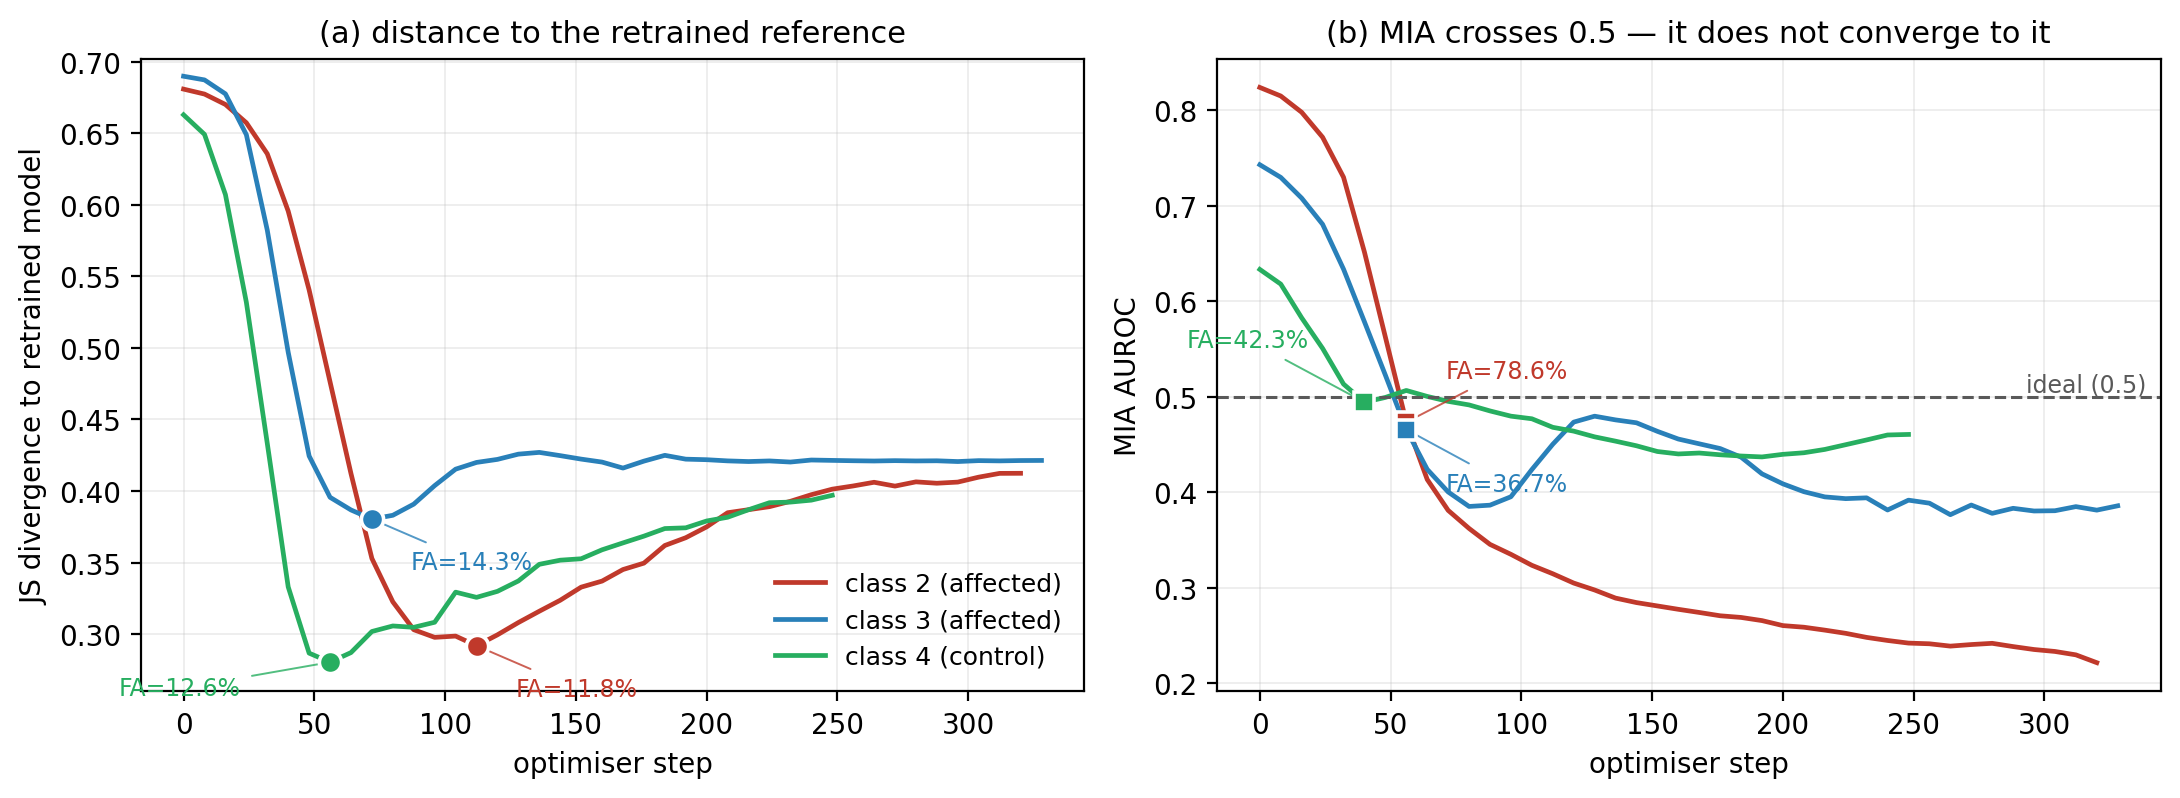
\includegraphics[width=\textwidth]{fig_trajectory.png}
\caption{\textbf{Unlearning overshoots the model it is trying to imitate, and
MIA cannot detect it.} \textbf{(a)}~Jensen--Shannon divergence to a
retrained-from-scratch reference along the unlearning trajectory. The curve is
U-shaped: the model first moves toward the reference, attains a minimum, then
moves away. Markers give the minimum, annotated with the forget accuracy there
($11.8$--$14.3\%$)---\emph{above} the $11.1\%$ chance level, whereas dual
stopping halts at ${\approx}7\%$. \textbf{(b)}~MIA AUROC on the same axis. It
sweeps \emph{through} the ideal $0.5$ rather than converging to it, so
$|\mathrm{MIA}-0.5|$ is minimised at the crossing. On class~2 that crossing
occurs while the model still classifies $78.6\%$ of the forget set
correctly.}
\label{fig:trajectory}
\end{figure}

\paragraph{The minimum is interior, and the current rule is past it.}
Divergence to the reference falls from $0.66$--$0.69$ at initialisation to
$0.28$--$0.38$, then rises again to $0.40$--$0.42$. So unlearning genuinely
moves the model toward a retrained one before moving away: over-forgetting is
not a metric artefact but a real overshoot in function space. The minimum lies
at $\mathrm{FA} = 11.8\%$, $14.3\%$ and $12.6\%$ for the three classes, while
dual stopping halts at ${\approx}7\%$ (\S\ref{sec:overforget}) --- past the
optimum in every case. Stopping at the minimum instead is close to free: test
accuracy changes by $-0.06$, $-0.03$ and $+0.79$pp and retain accuracy by
$+0.06$, $+0.36$ and $+0.08$pp. On the same trajectory it reduces divergence by
$0.016$, $0.003$ and $0.007$, and reduces $|\mathrm{MIA}-0.5|$ by $0.017$ and
$0.015$ on the two affected classes while moving the control by $+0.006$. This
is the pattern the criterion of \S\ref{sec:overforget} failed to produce:
the affected classes improve and the control stays put.

\paragraph{But the optimum is shallow, so we do not propose a numeric target.}
The three minima fall within $2.5$pp of one another in forget accuracy, which
invites the conclusion that ``stop at $\mathrm{FA}\approx 13\%$'' is a
deployable rule. The basin does not support that reading. Taking every
checkpoint within $5\%$ of the minimum divergence, the corresponding forget
accuracy spans $10.2$--$26.3\%$, $3.5$--$36.7\%$ and $6.9$--$21.9\%$ on the
three classes---$3.5$--$36.7\%$ overall. The agreement between the three
\emph{argmin} values is therefore largely a coincidence of where the snapshots
happened to land, and a single tuned number would not transfer. What the data
does support is directional and, we think, more useful: the optimum sits
\emph{above} the chance level, and a rule that drives forget accuracy to or
below chance is on the wrong side of it.

\paragraph{$|\mathrm{MIA}-0.5|$ is not an optimisation target.}
Panel~(b) is the more consequential finding. MIA AUROC does not converge to
$0.5$; it \emph{passes through} it, falling from $0.82$, $0.74$ and $0.63$ at
initialisation to $0.22$, $0.39$ and $0.46$ at the end. Consequently
$|\mathrm{MIA}-0.5|$ is minimised wherever the trajectory happens to cross,
which carries no information about unlearning quality. On class~2 the crossing
occurs at $\mathrm{FA} = 78.6\%$: a model that has barely forgotten anything
attains a \emph{perfect} MIA score. The two criteria also disagree about where
to stop, and in opposite directions---the divergence minimum and the MIA
minimum are $56$ steps apart on class~2, $56$ steps apart the other way on
class~3, and $8$ steps apart on class~4.

This sharpens the observation of \S\ref{sec:experiments} that a pre-unlearning
model already scores MIA $=0.533$. That was a single point; here we see the
whole path, and it shows that MIA $\approx 0.5$ is attainable at almost any
stage of unlearning, including stages with no meaningful forgetting at all.
Reporting MIA alongside forget accuracy is therefore not merely advisable but
necessary, and \emph{optimising} $|\mathrm{MIA}-0.5|$---which a practitioner
reading ``ideal $=0.5$'' might reasonably attempt---selects an arbitrary point
on the trajectory.

\paragraph{What remains unresolved.}
Stopping at the divergence minimum reduces over-forgetting without eliminating
it: class~2 still attains MIA $=0.315$ there, far from $0.5$. Nor do we have a
deployable rule, since locating the minimum requires the retrained reference
that unlearning exists to avoid, and the basin is too flat for a fixed forget
accuracy to stand in for it. We report the diagnosis---the stopping rule halts
on the wrong side of a real optimum---and leave a practical criterion open.
Whether the effect holds beyond the three PathMNIST classes measured here is
also untested; the experiment costs one unlearning run plus one retrained
reference per class.

% ============================================================
\section{Limitations in Full}\label{app:limitations}

\paragraph{Compute scales with classes and with data scarcity, and we cannot
predict it.} At \rev{its 15-epoch cap} \ours{} leaves STL-10 at
FA~$=75.7\%$, and an earlier version of this paper reported that as a failure
mode of the hard constraint on small forget sets. That diagnosis was wrong in
its conclusion though right about its cause. With 500 training images per class
the forget set yields only 4 mini-batches per epoch, ${\sim}60$ update steps in
total, and every step conflicts with the retain gradient---so progress per step
is small and the budget expires before forgetting completes. At 60 epochs, over
the same three seeds \rev{and with a per-step check and a $1\%$ target}, FA falls
to $1.73 \pm \rev{0.95}\%$ with RA~$=98.87\%$ \rev{(with the default $10\%$
target a single 60-epoch run stops at $9.2\%$)}. CIFAR-100
behaves the same way for a different reason: its per-class forget sets are small
because there are a hundred of them, and at 60 epochs its nine-class mean falls
from $4.07\%$ to $1.27 \pm \rev{0.39}\%$, bringing the $1\%$ chance level inside one
standard deviation. Neither constraint was infeasible; both runs were truncated.

What survives as a limitation is that we cannot say in advance how much budget a
new dataset needs. The binding resource is optimiser steps rather than epochs or
examples, and \ours{} offers no way to predict the requirement beyond monitoring
forget accuracy and continuing until the tolerance is met. A practitioner
deploying on an unfamiliar dataset should expect to discover the budget
empirically, and should treat a shared epoch count copied from another dataset
as a likely under-estimate.


\paragraph{Sample-level forgetting works, but at a cost the method cannot
control.} Every result in this paper removes a whole class. We tested the other
standard request type---forgetting a random subset of training points---on
CIFAR-10 at $1\%$ and $5\%$ of the training set, and report it as a scope limit
rather than a capability.

Two things go wrong, and they are different in kind. First, the forget objective
degenerates. \klr{} draws its power from the forget class being \emph{absent}
from the retain set, which drives $p_r$'s mass on that class to ${\sim}0$
(measured: $0.0002$); when the forget set is a random subset, the retain set
still covers every class and $p_r$ is uniform to three decimals
($0.100,0.100,\dots$). \klr{} therefore reduces exactly to
\texttt{kl\_uniform} in this regime, and the target carries no information about
\emph{which} points to forget. Second, dual stopping does not fire: the retain
budget is multiplicative on an initial retain loss of $0.0018$, so even at
$\alpha = 100$ both stopping-armed runs halted on the budget with forget accuracy
still at ${\sim}99.5\%$. A multiplicative budget is the wrong instrument against
a converged model; an absolute floor would be the right one.

Given a fixed 60-epoch budget and no stopping, forgetting does occur---forget
accuracy falls to $58.4\%$ at $1\%$ and $71.8\%$ at $5\%$---but
indiscriminately: retain accuracy falls from ${\sim}100\%$ to $73.2\%$ and test
accuracy to $71.9\%$, and forget accuracy ends \emph{below} test accuracy, which
is over-forgetting by the standard for this setting (a correctly unlearned point
should look like an unseen point of the same class, i.e.\ $\mathrm{FA}\approx
\mathrm{TA}$). The method has no mechanism to stop at that crossing.

The one clearly positive finding is the ablation. Removing the projection at
equal budget collapses the model completely: retain accuracy $14.2\%$ versus
$73.2\%$ with it, and test accuracy $17.1\%$ versus $71.9\%$---a $59$pp and
$55$pp difference respectively, far larger than the projection's effect in the
class-level ablation of Table~\ref{tab:ablation}. When forget and retain
gradients are drawn from the same distribution the conflict is near-total (the
projection fires on $100\%$ of steps), and the retain constraint is the only
thing keeping the model intact. The guarantee is therefore \emph{more}
load-bearing here, not less---which is why we regard sample-level forgetting as
a direction the constraint supports and the objective does not yet.

\paragraph{Mini-batch scope of the guarantee.} Theorem~\ref{thm:retain_safety}
bounds the \emph{sampled} retain objective---the quantity \ours{} projects
against---not the full-population retain loss. A population-exact per-step
guarantee would require controlling the gradient-variance term and is future
work.

\paragraph{The comparison with the closest prior work is structural, not
empirical.} Our separation from soft conflict-resolution methods
\citep{patel2025learning} rests on Theorem~\ref{thm:separation}(iv) and
Table~\ref{tab:properties}, both of which argue from the definition of the
update rule. We have not reimplemented that method and run it on our stack, so
we make no claim about how the two compare on accuracy, forgetting, or MIA. A
like-for-like empirical comparison is the most important piece of missing
evidence in this paper. Two related experiments are reported and should not be
mistaken for it: the projection-only ablation, isolating the projection from
\ours{}'s other three components (Table~\ref{tab:cifar10}), and the
projection-strength sweep, which interpolates our own update between a soft
penalty and the hard constraint (\S\ref{sec:strength}). Both test the mechanism;
neither runs the cited method.

\paragraph{Floating-point exactness.} The guarantee holds to float32 precision
(\S\ref{sec:alignment}); exact arithmetic would require float64 inner products.

\added{\paragraph{BatchNorm robustness is bought with compute, and is scoped.}
BN-robust \ours{} (\S\ref{sec:bn_robust}) survives the recalibration attack at
about seven times the wall-clock of the default configuration, because forgetting
that has to happen in the weights takes more steps. It was evaluated on two
datasets, CIFAR-10 (every class) and MNIST, and on base models that differ from
those behind the rest of the paper. It also defends only the normalisation
statistics: an attacker who modifies weights, as in the fine-tuning recovery
below, is outside what it changes.}

\paragraph{\rev{Sequential unlearning and fine-tuning recovery.}}
\rev{\emph{Sequential unlearning}: forgetting classes $0$, then $1$, then $2$
from each resulting checkpoint takes test accuracy $86.1 \to 76.8 \to 69.1$ and
retain accuracy $100.0 \to 89.7 \to 80.7$, with forget accuracy on the newest
class at most $2.7\%$. The decline is what forgetting does to these metrics,
not damage. TA counts every forgotten class's test images as errors, so fully
forgotten classes alone take it to $0.9$, $0.8$ and $0.7$ times the
retained-class accuracy (with the base model's $95.5\%$: $86.0$, $76.4$ and
$66.9\%$); RA is measured on a retain set that still contains the
earlier-forgotten classes, so fully forgotten classes take it to at most $8/9$
and $7/9$ ($88.9\%$ and $77.8\%$). The observed values sit at or above these
levels, so the retained classes are not damaged cumulatively. They sit above
them because earlier-forgotten classes partly return: an RA of $80.7\%$ requires
the two earlier classes to average at least $13\%$ training accuracy, above the
$10\%$ chance level. A sequential deployment should therefore re-check every
forgotten class after each request.} \emph{Fine-tuning recovery}: retraining the unlearned model on
$50$ forget-class samples raises forget accuracy from $1.9\%$ to $7.1\%$ after
five epochs and $51.3\%$ after ten---though by then the model is no longer
usable ($\mathrm{TA} = 34.6\%$, $\mathrm{RA} = 47.9\%$), so the attack recovers
the class only by destroying the model it attacks. \ours{} also does not provide
formal $(\varepsilon,\delta)$-DP guarantees.

\section{Per-Class Results}\label{app:perclass}

The main text reports per-dataset aggregates (Table~\ref{tab:cross}). Because a
mean over classes can conceal a method that succeeds on easy classes and fails on
hard ones, we report every class individually. Each row is the mean $\pm$
standard deviation over seeds $\{42,123,456\}$. CIFAR-100 per-class results
appear in the main text (Table~\ref{tab:cifar100}); the raw per-run CSVs for all
75 runs are released with the code.

\begin{figure}[t]
\centering
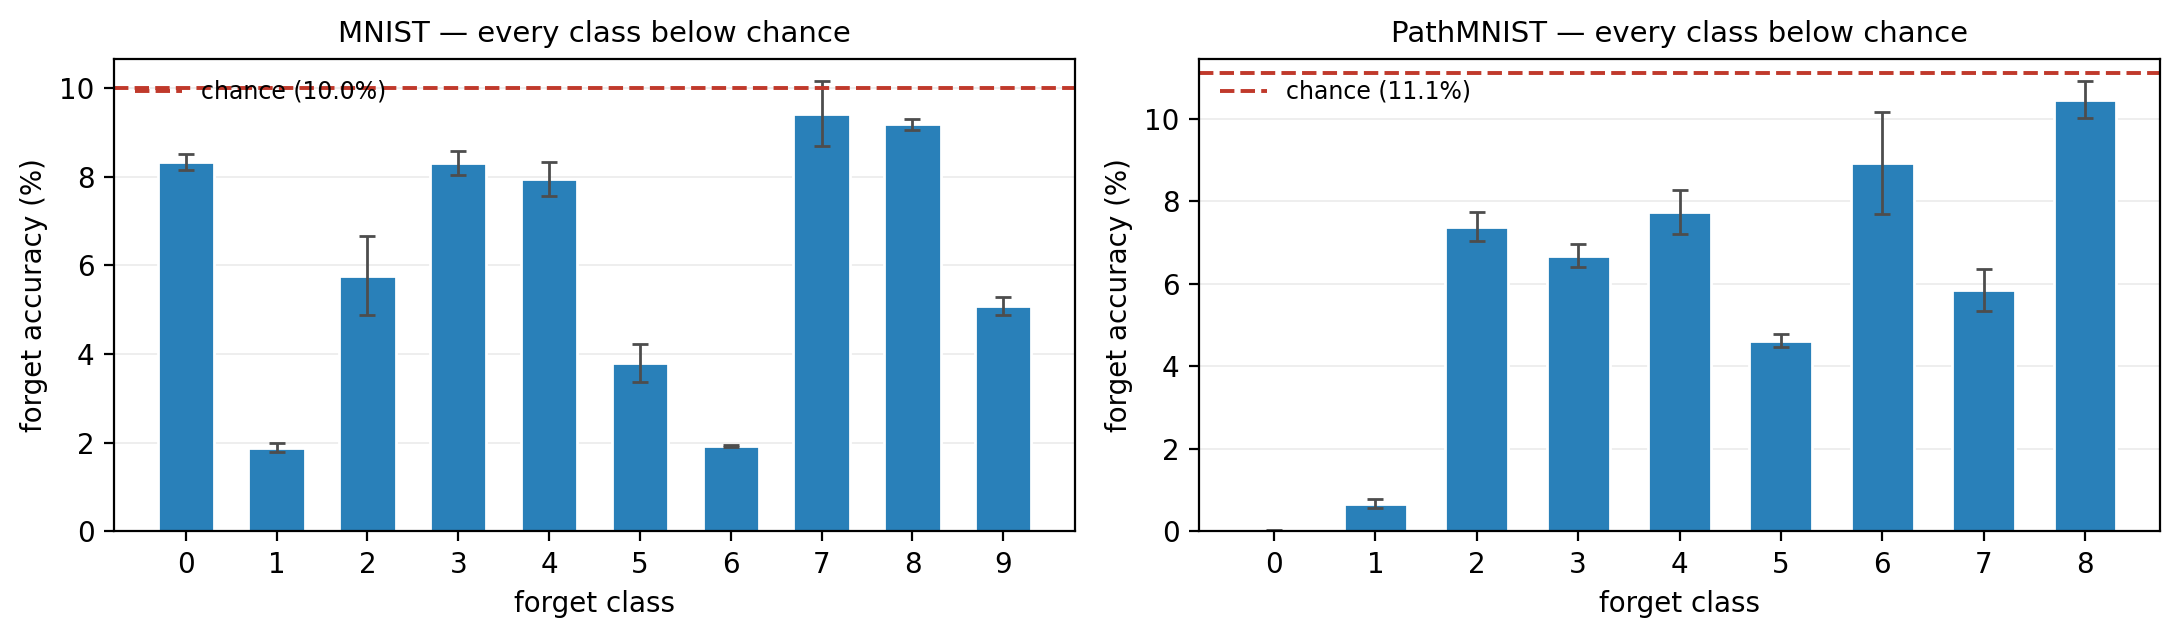
\includegraphics[width=\textwidth]{fig_perclass.png}
\caption{\textbf{Per-class forget accuracy} (mean $\pm$ std over three seeds).
Every MNIST and PathMNIST class individually falls below its chance level, so
the per-dataset means of Table~\ref{tab:cross} are not concealing a class that
fails.}
\label{fig:perclass}
\end{figure}

\subsection{MNIST (all 10 classes)}

Table~\ref{tab:app_mnist} gives all ten MNIST classes. Every class individually
falls below the $10\%$ chance level, with per-class mean FA ranging from
$1.89\%$ (class~1) to $9.42\%$ (class~7); the aggregate is therefore not
concealing a failure. Retain accuracy is essentially constant across classes
($99.42$--$99.54\%$), and MIA stays within $0.017$ of the ideal $0.5$ for every
class. Seed variance is small throughout (the largest FA standard deviation
across classes is $0.89$pp), indicating the procedure is stable rather than
seed-lucky.

\begin{table}[t]
\centering
\caption{\textbf{MNIST per-class forgetting} (mean $\pm$ std over 3 seeds).
Chance level is $10.0\%$; every class attains FA below it. TA is measured on the
full test set, so it necessarily drops by ${\sim}10$pp relative to the
$99\%$ base model once the forget class is correctly no longer recognised.}
\label{tab:app_mnist}
\begin{tabular}{@{}ccccc@{}}
\toprule
Forget class & TA (\%) & FA (\%)$\downarrow$ & RA (\%) & MIA \\
\midrule
0 & $90.26 \pm 0.05$ & $8.33 \pm 0.18$ & $99.42 \pm 0.00$ & $0.495 \pm 0.002$ \\
1 & $88.29 \pm 0.01$ & $1.89 \pm 0.09$ & $99.50 \pm 0.02$ & $0.512 \pm 0.001$ \\
2 & $89.68 \pm 0.07$ & $5.77 \pm 0.89$ & $99.51 \pm 0.01$ & $0.491 \pm 0.001$ \\
3 & $90.37 \pm 0.02$ & $8.31 \pm 0.27$ & $99.45 \pm 0.01$ & $0.483 \pm 0.001$ \\
4 & $90.22 \pm 0.01$ & $7.95 \pm 0.39$ & $99.43 \pm 0.02$ & $0.510 \pm 0.001$ \\
5 & $90.76 \pm 0.04$ & $3.80 \pm 0.43$ & $99.52 \pm 0.03$ & $0.499 \pm 0.001$ \\
6 & $90.08 \pm 0.02$ & $1.92 \pm 0.03$ & $99.50 \pm 0.02$ & $0.501 \pm 0.001$ \\
7 & $90.03 \pm 0.03$ & $9.42 \pm 0.74$ & $99.51 \pm 0.01$ & $0.490 \pm 0.000$ \\
8 & $90.36 \pm 0.03$ & $9.19 \pm 0.13$ & $99.50 \pm 0.02$ & $0.486 \pm 0.001$ \\
9 & $89.97 \pm 0.05$ & $5.09 \pm 0.21$ & $99.54 \pm 0.02$ & $0.503 \pm 0.000$ \\
\midrule
\textbf{Mean} & $\mathbf{90.00}$ & $\mathbf{6.17}$ & $\mathbf{99.49}$ & $\mathbf{0.497}$ \\
\bottomrule
\end{tabular}
\end{table}

\subsection{PathMNIST (all 9 classes)}

Table~\ref{tab:app_pathmnist} gives all nine PathMNIST tissue classes. Every
class again falls below the $11.1\%$ chance level, from $0.02\%$ (class~0) to
$10.46\%$ (class~8). Two observations deserve stating explicitly rather than
being averaged away.

First, the spread is far wider than on MNIST---per-class TA ranges from
$73.23\%$ to $89.28\%$---reflecting genuinely unequal class difficulty in
histopathology rather than instability: within-class seed variance remains small
(largest FA standard deviation $1.23$pp).

Second, and more importantly, \textbf{MIA AUROC is not uniformly near $0.5$}:
class~2 reaches $0.298$ and class~3 $0.388$, both well \emph{below} the ideal.
A value substantially below $0.5$ indicates that forget-class training samples
have become \emph{harder} to classify than forget-class test samples---the
signature of \emph{over}-forgetting, in which the unlearned model is
distinguishable from a retrained one in the opposite direction to a privacy
leak. It is detectable precisely because we report MIA per class and treat
distance from $0.5$ in either direction as a defect. We flag this as a real
limitation of the current stopping rule on PathMNIST: dual stopping targets FA,
which does not constrain how far past the retrained model's output statistics the
optimiser travels.

\begin{table}[t]
\centering
\caption{\textbf{PathMNIST per-class forgetting} (mean $\pm$ std over 3 seeds).
Chance level is $11.1\%$; every class attains FA below it. $^{\dagger}$Classes~2
and~3 show MIA well below the ideal $0.5$, indicating over-forgetting (see
text).}
\label{tab:app_pathmnist}
\begin{tabular}{@{}ccccc@{}}
\toprule
Forget class & TA (\%) & FA (\%)$\downarrow$ & RA (\%) & MIA \\
\midrule
0 & $73.23 \pm 0.06$ & $0.02 \pm 0.02$ & $99.01 \pm 0.01$ & $0.511 \pm 0.003$ \\
1 & $78.66 \pm 0.26$ & $0.68 \pm 0.12$ & $98.48 \pm 0.08$ & $0.473 \pm 0.003$ \\
2$^{\dagger}$ & $89.28 \pm 0.12$ & $7.38 \pm 0.35$ & $99.02 \pm 0.02$ & $0.298 \pm 0.003$ \\
3$^{\dagger}$ & $82.40 \pm 0.12$ & $6.68 \pm 0.28$ & $98.86 \pm 0.02$ & $0.388 \pm 0.005$ \\
4 & $78.04 \pm 0.08$ & $7.73 \pm 0.53$ & $98.95 \pm 0.03$ & $0.502 \pm 0.001$ \\
5 & $84.58 \pm 0.03$ & $4.62 \pm 0.15$ & $98.32 \pm 0.02$ & $0.548 \pm 0.001$ \\
6 & $78.58 \pm 0.25$ & $8.93 \pm 1.23$ & $98.77 \pm 0.06$ & $0.541 \pm 0.001$ \\
7 & $88.48 \pm 0.14$ & $5.85 \pm 0.50$ & $99.25 \pm 0.01$ & $0.562 \pm 0.001$ \\
8 & $75.36 \pm 0.04$ & $10.46 \pm 0.45$ & $99.28 \pm 0.03$ & $0.525 \pm 0.001$ \\
\midrule
\textbf{Mean} & $\mathbf{80.96}$ & $\mathbf{5.82}$ & $\mathbf{98.88}$ & $\mathbf{0.483}$ \\
\bottomrule
\end{tabular}
\end{table}

\paragraph{On the per-dataset MIA aggregate.}
The PathMNIST aggregate of $0.483 \pm 0.084$ in Table~\ref{tab:cross} is within
$0.017$ of ideal, but its standard deviation is an order of magnitude larger
than any other dataset's precisely because of classes~2 and~3. The aggregate is
accurate but uninformative here; this is a concrete instance of the more general
point of \S\ref{sec:experiments} that MIA must be read alongside FA, and
per-class rather than only in aggregate.

\begingroup\color{revised}% ---- new appendix subsection: added up to \endgroup
\subsection{BN-robust \ours{} on all ten CIFAR-10 classes}\label{app:bnrobust_perclass}

Table~\ref{tab:app_bnrobust} gives every CIFAR-10 class under the recalibration
attack of \S\ref{sec:bn_robust}, one seed per class (class~0 has three seeds in
Table~\ref{tab:bnrobust}). ``Pre'' and ``post'' are FA under test-time transforms
before and after \texttt{update\_bn} on the retain set. All runs share the
$93.97\%$ base of \S\ref{sec:bn_robust}. The calibrated runs here read the
stopping FA on the full retain set rather than the $10{,}240$-image subset; on
class~0 the two made identical stopping decisions (\S\ref{sec:bn_robust}).

\begin{table}[t]
\centering\color{revised}
\caption{\added{\textbf{BN-robust \ours{} per class} (CIFAR-10, seed~$42$). The
frozen-statistics configuration is recovered on every class. BN-robust is not,
under either stopping rule, and with calibrated stopping every class ships within
three standard errors of chance ($11.3\%$). Epochs ``$25{\to}22$'': the run
reached the cap and its best epoch was shipped.}}
\label{tab:app_bnrobust}
\small
\setlength{\tabcolsep}{4pt}
\begin{tabular}{@{}cccccccccc@{}}
\toprule
& \multicolumn{2}{c}{Frozen} & \multicolumn{2}{c}{BN-robust, naive}
& \multicolumn{5}{c}{BN-robust, calibrated} \\
\cmidrule(lr){2-3}\cmidrule(lr){4-5}\cmidrule(l){6-10}
Class & pre & post & pre & post & pre & post & epochs & TA & RA \\
\midrule
0 & $8.76$ & $99.22$ & $9.24$ & $9.28$ & $9.22$ & $9.24$ & 13 & $84.35$ & $95.60$ \\
1 & $2.40$ & $97.60$ & $10.66$ & $10.66$ & $6.66$ & $6.66$ & 8 & $84.56$ & $96.19$ \\
2 & $6.52$ & $98.30$ & $11.18$ & $11.16$ & $9.90$ & $9.92$ & 15 & $85.07$ & $95.27$ \\
3 & $4.78$ & $94.82$ & $11.30$ & $11.30$ & $10.00$ & $9.98$ & 16 & $85.92$ & $96.26$ \\
4 & $4.84$ & $97.34$ & $13.32$ & $13.34$ & $10.18$ & $10.16$ & $25{\to}22$ & $84.88$ & $94.74$ \\
5 & $7.28$ & $94.70$ & $8.78$ & $8.78$ & $9.40$ & $9.42$ & 12 & $84.52$ & $94.64$ \\
6 & $9.18$ & $99.14$ & $7.20$ & $7.20$ & $7.30$ & $7.30$ & 8 & $83.32$ & $94.41$ \\
7 & $3.38$ & $96.20$ & $11.36$ & $11.34$ & $9.12$ & $9.12$ & 10 & $84.49$ & $95.24$ \\
8 & $4.54$ & $99.26$ & $16.74$ & $16.68$ & $9.74$ & $9.68$ & 14 & $83.59$ & $94.67$ \\
9 & $2.52$ & $98.16$ & $15.44$ & $15.42$ & $8.92$ & $8.92$ & 11 & $83.84$ & $95.01$ \\
\midrule
Mean & $5.42$ & $97.47$ & $11.52$ & $11.52$ & $9.04$ & $9.04$ & --- & $84.45$ & $95.20$ \\
\bottomrule
\end{tabular}
\end{table}

\begin{figure}[t]
\centering\color{revised}
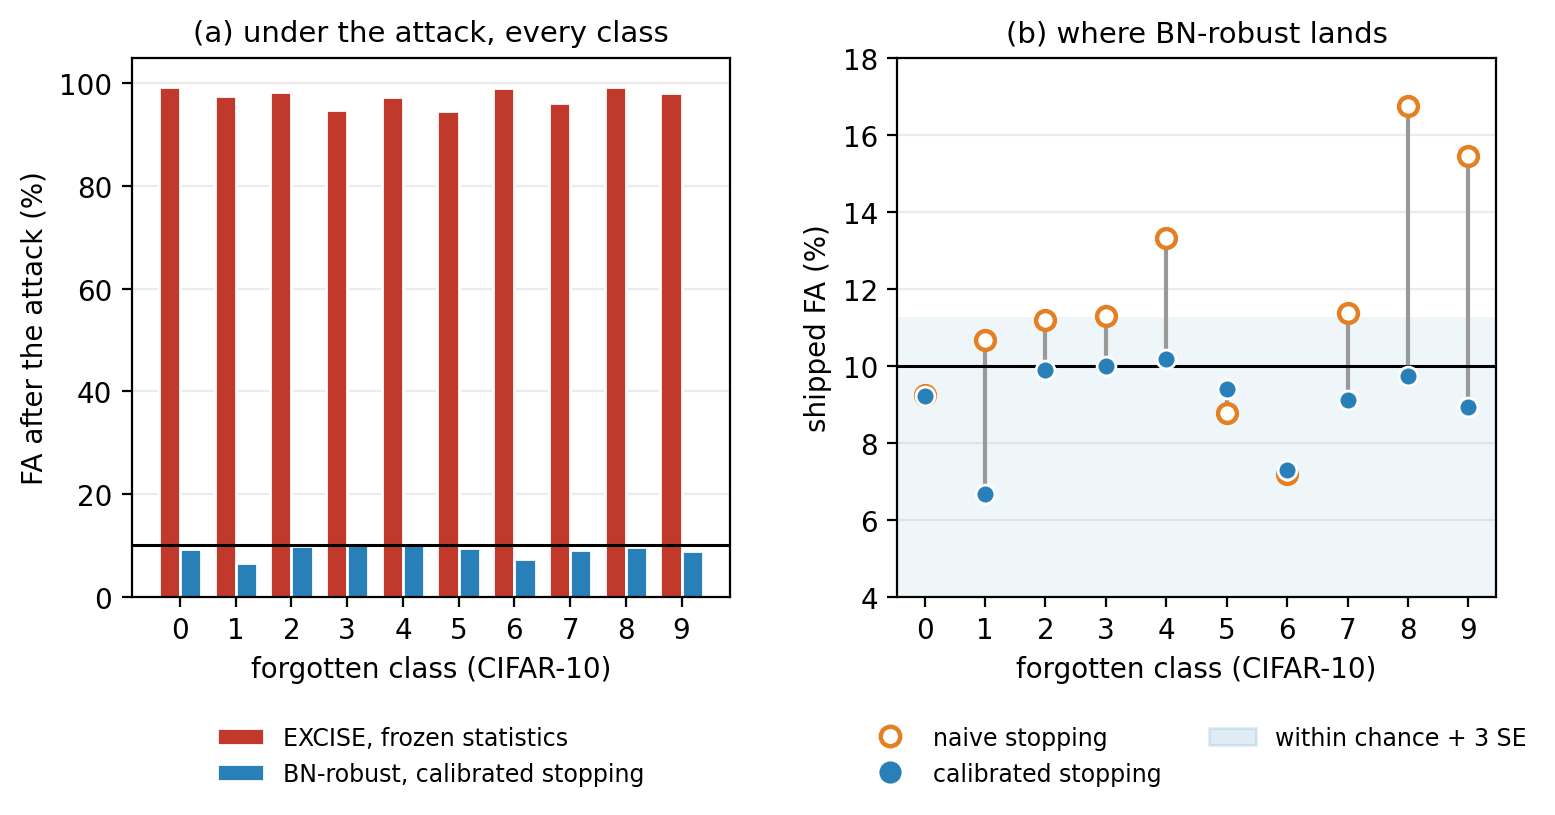
\includegraphics[width=\textwidth]{fig_bnrobust_perclass.png}
\caption{\added{\textbf{BN-robust on all ten CIFAR-10 classes} (seed~$42$; the data of
Table~\ref{tab:app_bnrobust}). (a)~Under the attack, the frozen-statistics
configuration is recovered on every class and BN-robust on none. (b)~Where
BN-robust ships: with naive stopping (open) five classes land above chance
$+\,3$\,SE; with calibrated stopping (filled), none do.}}
\label{fig:app_bnrobust}
\end{figure}
\endgroup% ---- end of the added appendix subsection

% ------------------------------------------------------------
\section{Hyperparameter Configuration}\label{app:hyper}

Table~\ref{tab:app_shared} lists the settings shared across all datasets and
Table~\ref{tab:app_perdataset} the per-dataset settings. All are released as YAML
configuration files; the reported runs use them unmodified.

\begin{table}[t]
\centering
\caption{\textbf{Shared hyperparameters} (identical for all six datasets). The
two components removed from \ours{} are listed explicitly with value $0$, since
they remain available as flags for the ablation of \S\ref{sec:ablation}.}
\label{tab:app_shared}
\begin{tabular}{@{}llll@{}}
\toprule
Symbol & Flag & Value & Role \\
\midrule
$\mu$ & \texttt{--momentum} & $0.9$ & momentum; projection applied \emph{after} accumulation \\
$c$ & \texttt{--max\_grad\_norm} & $1.0$ & clip on $d_t$, \emph{before} accumulation \\
$\lambda_{\mathrm{wd}}$ & \texttt{--weight\_decay} & $5\times10^{-4}$ & weight decay, applied inside $d_t$ \\
$T_{\mathrm{KD}}$ & \texttt{--temperature} & $4.0$ & distillation temperature \\
--- & \texttt{--forget\_objective} & \klr{} & KL toward retain-confusion $p_r$ \\
--- & \texttt{--batch\_size} & $128$ & forget and retain mini-batch size \\
--- & \texttt{--fa\_check\_freq} & $50$ & intra-epoch FA check interval (batches) \\
--- & \texttt{--seed} & $\{42,123,456\}$ & three seeds per task \\
\midrule
\multicolumn{4}{@{}l}{\emph{Removed components (retained as ablation flags only)}} \\
$\lambda$ & \texttt{--rep\_weight} & $0.0$ & representation erasure (removed) \\
$\gamma$ & \texttt{--forget\_gate} & $0.0$ & entropy gate (removed) \\
\bottomrule
\end{tabular}
\end{table}

\begin{table}[t]
\centering
\caption{\textbf{Per-dataset hyperparameters.} $K$ is the number of classes.
Note that the forget-accuracy target $\tau_F$ is set to the chance level
$100/K$ for every dataset---it is not tuned per dataset, but derived from the
task.}
\label{tab:app_perdataset}
\begin{tabular}{@{}lcccccc@{}}
\toprule
Dataset & $K$ & Epochs $T$ & $\eta$ & $\beta$ (KD) & $\alpha$ (retain budget) & $\tau_F = 100/K$ \\
\midrule
CIFAR-10  & 10  & 15 & $5\times10^{-4}$ & $2.0$ & $5.0$ & $10.0\%$ \\
CIFAR-100 & 100 & 20 & $5\times10^{-4}$ & $2.0$ & $5.0$ & $\phantom{0}1.0\%$ \\
MNIST     & 10  & 12 & $2\times10^{-4}$ & $3.0$ & $4.0$ & $10.0\%$ \\
SVHN      & 10  & 15 & $2\times10^{-4}$ & $3.0$ & $5.0$ & $10.0\%$ \\
STL-10    & 10  & 15 & $2\times10^{-4}$ & $5.0$ & $5.0$ & $10.0\%$ \\
PathMNIST & \phantom{0}9 & 12 & $2\times10^{-4}$ & $5.0$ & $4.0$ & $11.1\%$ \\
\bottomrule
\end{tabular}
\end{table}

\paragraph{Tuning effort.}
Only four quantities vary across datasets: the epoch cap $T$, the learning rate
$\eta$, the KD weight $\beta$, and the retain budget $\alpha$. The learning rate
takes one of two values ($5\times10^{-4}$ for the CIFAR datasets,
$2\times10^{-4}$ elsewhere), $\beta$ one of three, and $\alpha$ one of two. The
forget target $\tau_F$ is not tuned at all: it is fixed to the chance level
$100/K$ implied by the task. Notably, $\mu$, $c$, $\lambda_{\mathrm{wd}}$, and
$T_{\mathrm{KD}}$---the four quantities that enter the guarantee of
Theorem~\ref{thm:app_main}---are held constant across all six datasets, so the
bound $\tfrac12 L\eta^2(c/(1-\mu))^2$ varies across datasets only through
$\eta$ (and through the dataset-dependent smoothness constant $L$).

\paragraph{A note on defaults.}
The command-line default for \texttt{--max\_grad\_norm} in the released code is
$5.0$, whereas every configuration file sets $c=1.0$. Runs launched without
\texttt{--config} would therefore use a different clip threshold, and a
correspondingly weaker constant in
(\ref{eq:app_c}). All results in this paper use the configuration files. We note
this because the value of $c$ enters the guarantee directly, so it should not be
inherited silently from a default.

% ------------------------------------------------------------
\section{Distance to the Retrained Model: A Refuted Hypothesis}\label{app:d2r}

This appendix reports a negative result. We formed a hypothesis about why
\ours{} over-forgets on two PathMNIST classes, derived a deployable fix from it,
pre-committed to a falsifiable prediction, ran the experiment, and the
prediction did not hold. We report it in full because the experiment also
produced the diagnosis that we believe is correct, and because the refuted
hypothesis concerns \ours{}'s own forget objective.

\subsection{The defect, and the hypothesis}

Per-class reporting (Appendix~\ref{app:perclass}) showed that on PathMNIST
classes~2 and~3, MIA AUROC reaches $0.298$ and $0.388$---far \emph{below} the
ideal $0.5$. Forget accuracy is satisfied on both, so FA alone certifies these
runs as successes when they are not. A value below $0.5$ means forget-class
training samples have become \emph{harder} to classify than forget-class test
samples: the model is still distinguishable from a retrained one, in the
opposite direction to a privacy leak.

\rev{An earlier version of our forget-side condition (Eq.~\ref{eq:problem}) was
$\KL(p_\theta(x_f)\,\|\,p_r) \le \epsilon$}, a statement about
\emph{distributions}, but dual stopping (\S\ref{sec:stopping}) implements
\rev{$\mathrm{FA} \le \tau_F$}, a statement about \emph{argmax}. These are not
equivalent, and we hypothesised that the discrepancy was the cause: FA cannot
distinguish (a)~$p_\theta(x_f)$ having moved \emph{to} the distribution a
retrained model produces from (b)~having moved \emph{past} it, since both give
$\mathrm{FA}\approx 0$.

The hypothesised fix was to enforce the constraint as stated. Since $p_r$ is
computed from the \emph{original} model, this needs no retrained reference and
is deployable: stop on $\KL(p_\theta(x_f)\|p_r)$ rather than on FA. We reasoned
that this quantity is minimised at $p_\theta = p_r$ and rises on either side, so
a stop-when-it-stops-improving rule would halt at the minimum---exactly the
point FA cannot locate.

\paragraph{Prediction (pre-committed).} Replacing FA stopping with KL stopping
would, on the affected classes, (1)~reduce $|\mathrm{MIA}-0.5|$, (2)~reduce
Jensen--Shannon divergence to a retrained reference, and (3)~not materially
worsen FA or RA, while leaving an unaffected control class approximately
unchanged.

\subsection{Design}

We retrained reference models without the forget class for PathMNIST classes~2
and~3 (affected) and class~4 (control, MIA already $0.501$), keeping all $K$
output heads so that output distributions remain comparable, and training all
three identically for a fixed 30-epoch cosine schedule so that no reference is
better converged than another. Arm~A is \ours{} with FA stopping (the deployed
configuration); arm~B disables FA stopping and enables KL stopping. Oracle
metrics are computed against the references: JS divergence between output
distributions on the forget set (primary), top-1 agreement with the reference,
Fr\'echet distance between penultimate features, and MIA.

The control class is the load-bearing part of the design: a criterion that
merely stops earlier everywhere would improve the affected classes while also
perturbing the control, whereas a targeted fix should leave the control alone.

\subsection{Result: the prediction fails}

Table~\ref{tab:app_klstop} reports the outcome. Across three classes and four
metrics, arm~B is better on 2 comparisons and worse on 10. The primary oracle
metric---JS divergence to the retrained model---is \emph{worse in all three
classes}. The control class degrades on every metric, which is precisely the
signature that rules out a targeted fix. Only class~3 improves on
$|\mathrm{MIA}-0.5|$.

\begin{table}[t]
\centering
\caption{\textbf{KL stopping vs.\ FA stopping on PathMNIST}, measured against
retrained references. Arrows mark the direction of improvement. The prediction
was that the affected classes would improve and the control would not move;
neither held.}
\label{tab:app_klstop}
\begin{tabular}{@{}llccccc@{}}
\toprule
Class & Arm & $|\mathrm{MIA}{-}0.5|\downarrow$ & JS$\downarrow$ &
agree \%$\uparrow$ & Fr\'echet$\downarrow$ & $\KL$ to $p_r$ \\
\midrule
\multirow{2}{*}{2 (affected)}
 & FA stop & $0.205$ & $0.308$ & $45.4$ & $185.7$ & $0.957$ \\
 & KL stop & $0.268$ & $0.412$ & $23.5$ & $332.0$ & $0.052$ \\
\midrule
\multirow{2}{*}{3 (affected)}
 & FA stop & $0.115$ & $0.382$ & $31.2$ & $375.2$ & $0.805$ \\
 & KL stop & $\mathbf{0.068}$ & $0.421$ & $\mathbf{39.8}$ & $780.1$ & $0.002$ \\
\midrule
\multirow{2}{*}{4 (control)}
 & FA stop & $0.001$ & $0.286$ & $38.7$ & $141.1$ & $1.510$ \\
 & KL stop & $0.044$ & $0.399$ & $12.3$ & $297.7$ & $0.116$ \\
\bottomrule
\end{tabular}
\end{table}

\paragraph{The proxy is anti-correlated with the oracle.}
A proxy is only usable if it tracks the quantity it stands in for. Across the
six checkpoints, the rank correlation between $\KL(p_\theta\|p_r)$ and JS
divergence to the retrained model is $\rho = -1.00$ (Pearson $-0.94$): the
ordering is perfectly inverted. Driving the deployable proxy toward zero moves
the model monotonically \emph{away} from the retrained reference. This is the
opposite of the relationship the hypothesis required.

\subsection{Why it failed}

\paragraph{(i) The criterion never fired.}
In all three runs of arm~B the terminating condition was the retain-loss budget,
not the KL rule. The reason is visible in the logged trajectories:
$\KL(p_\theta(x_f)\|p_r)$ decreases essentially monotonically (class~2:
$5.53 \to 0.05$ over 8 checks with zero increases; class~4: $2.73 \to 0.07$,
zero increases; class~3: $2.06 \to 0.002$ over 20 checks with 4 small
increases). It never turns back up, so a stop-when-it-stops-improving rule
cannot trigger. The U-shape the hypothesis assumed does not exist over the
range the optimiser traverses.

This is also a limitation of the test, and we state it plainly: because the KL
rule never fired and FA stopping was disabled, arm~B is in effect \ours{}
\emph{without forget-side stopping} (FA reaches $0.0$ in all three runs), which
is closer to the $-$Stopping ablation than to a KL-stopped method. The
comparison in Table~\ref{tab:app_klstop} is therefore evidence against the
criterion \emph{as specified}, not a clean contrast between two stopping rules.

\paragraph{(ii) $p_r$ is a global average; a retrained model routes per-sample.}
$p_r$ is a single distribution, the retain-set average softmax, and it is the
same target for every forget sample. A retrained model does something different:
it routes each forget-class image to whichever surviving class that particular
image most resembles, giving an input-dependent output distribution. Matching
$p_r$ more closely therefore makes the model's predictions on forget data
unnaturally homogeneous across samples. The agreement column is the evidence:
as $\KL$ to $p_r$ falls by one to three orders of magnitude, top-1 agreement
with the reference \emph{collapses} on two of the three classes
($45.4 \to 23.5$ on class~2, $38.7 \to 12.3$ on class~4). If $p_r$ were the
right target, matching it better should have raised agreement. Class~3 moves the
other way ($31.2 \to 39.8$), so the effect is not universal.

\paragraph{Confound we cannot separate.}
$\KL$ to $p_r$ decreases with training time while JS to the reference increases
over the observed range, so the two are mechanically anti-correlated and the
$\rho = -1.00$ figure partly reflects run duration rather than target quality
alone. The agreement collapse is the part of the evidence that speaks to the
target itself, and it rests on two of three classes. We therefore claim the
criterion is refuted, and treat the mechanism as well-supported but not
established.

\subsection{What the experiment did establish}

\paragraph{The FA rule overshoots its own target.}
All three FA-stopped runs halt at $\mathrm{FA} \approx 7\%$ against a target of
$11.1\%$ (the chance level), overshooting by $3.9$--$4.2$pp, because the
intra-epoch FA check is evaluated only every 50 batches. The over-forgetting we
set out to explain is thus at least partly a \emph{granularity} defect in how
the existing criterion is enforced, not evidence that FA is the wrong quantity.

\paragraph{Less unlearning was better on every class.}
JS divergence to the retrained model is lower at the earlier stopping point in
all three classes. Over the range we observe, the model is still moving toward
the retrained reference when FA stopping halts it, and continues away from it
afterwards. Combined with the overshoot above, this points to stopping
\emph{earlier and more precisely} rather than to replacing the stopped quantity.

\paragraph{Consequence for the method.}
We draw a narrower conclusion about \klr{} than the original formulation
implies. As a forget-side \emph{direction}, $p_r$ is a better target than the
uniform distribution (\S\ref{sec:forget_obj}). As a \emph{target to be minimised
to zero}, it is actively harmful. \rev{Accordingly Eq.~\ref{eq:problem} states
the forget condition on forget accuracy and uses the divergence only as the
direction of the search}, and we do not claim $p_r$ is what a retrained model produces on forget
inputs---the measurements here show it is not.

\subsection{Open question}

Where JS divergence to the retrained model is minimised along the unlearning
trajectory remains unmeasured. Since JS is still falling when FA stopping fires
and rising afterwards, a minimum exists between the base model and the FA-stopped
point; locating it would establish whether a single FA level identifies it across
classes, which would make it deployable, or whether it varies per class, which
would not.
This question is answered in \S\ref{sec:trajectory}: the minimum is interior, lies above the chance level, and the current rule stops past it.

% ------------------------------------------------------------
\section{Ethical and Societal Considerations}\label{app:ethics}

\paragraph{Unlearning as evidence removal.}
A method that makes a model indistinguishable from one retrained without
specific data could be misused to destroy evidence that problematic data was
used for training. This is a dual-use property of the unlearning goal itself
rather than of \ours{} specifically, but \ours{} does make it concrete. Partial
mitigation is that \ours{} leaves an audit trail by construction: projection-rate
logs, the FA trajectory, and retain-loss budget history are all recorded per run,
so an auditor with access to the logs can establish that unlearning was applied
and to what extent. We note this is mitigation, not prevention---an adversary who
controls the logs controls the audit.

\paragraph{Selective fairness degradation.}
Class-level unlearning removes all samples of a class, which may correspond to a
demographic group. Crucially, the accuracy degradation we observe is
\emph{not} confined to the forgotten class: test accuracy falls beyond what the
removed class alone accounts for, and the per-class spread on PathMNIST
(Appendix~\ref{app:perclass}) shows the effect is uneven across classes.
Deployers should therefore monitor per-class accuracy before and after
unlearning rather than only aggregate accuracy, which can conceal a
disproportionate cost borne by one group.

\paragraph{Over-forgetting as a distinct harm.}
The PathMNIST finding (Appendix~\ref{app:perclass}) shows that a model can be
pushed \emph{past} the retrained reference. This matters ethically as well as
technically: such a model is still distinguishable from one trained without the
data, so a deletion request has not been faithfully honoured, yet every
FA-based check reports success. Compliance evidence resting on forget accuracy
alone would be misleading here.

\paragraph{Regulatory gap.}
Approximate unlearning methods, including \ours{}, do not satisfy formal
$(\varepsilon,\delta)$-differential-privacy certification. Whether
MIA AUROC~$\approx 0.5$ constitutes legally sufficient ``erasure'' under
instruments such as the GDPR right to erasure remains an open legal question on
which we take no position. The per-step guarantee of
Theorem~\ref{thm:retain_safety} is a statement about \emph{retain-side utility},
not a privacy certificate, and should not be presented as one.

% ------------------------------------------------------------
\section{Reproducibility}\label{app:repro}

\paragraph{Artefacts.}
Code, YAML configuration files, per-run summary CSVs for all 75 runs, and the
BatchNorm-recalibration diagnostic are released in the anonymised repository.
\todo{Insert the anonymised repository URL.}
The archived $\mu=0$ results underlying Table~\ref{tab:momentum} are released
alongside the main results, so the momentum ablation can be re-derived without
re-running it.

\paragraph{Environment.}
PyTorch $\ge 2.0$ with CUDA; ResNet-18 (11.7M parameters) throughout. Runs were
executed on a single GPU. Datasets download automatically except PathMNIST,
which is obtained through \texttt{medmnist}.

\paragraph{Implementation details that affect results.}
\begin{itemize}
\item Momentum and weight decay are applied \emph{manually} so that the
projection acts on the post-momentum update; the underlying \texttt{torch} SGD
object is configured with \texttt{momentum=0}, \texttt{weight\_decay=0} and acts
only as a plain step. Reading the optimiser construction alone is therefore
misleading---see \S\ref{sec:optimiser} and Appendix~\ref{app:setup}.
\item Clipping is applied to $d_t$ before momentum accumulation, and \emph{not}
to the final update. Reversing this changes the effective step size by a factor
$1/(1-\mu)$ (Proposition~\ref{prop:clip}).
\item The projected update is rescaled to the pre-projection norm.
\item BatchNorm layers are set to \texttt{eval()} immediately after the model is
set to \texttt{train()}, so running statistics are frozen during unlearning.
\added{BN-robust \ours{} (\S\ref{sec:bn_robust}) instead recomputes them from
$512$ retain images before every step (\texttt{--bn\_robust exact
--bn\_recal\_samples 512}) and on the full retain set under test-time transforms
after the last step. It reads the stopping forget accuracy under statistics
recomputed from $10{,}240$ retain images (\texttt{--bn\_calibrated\_stop
--bn\_stop\_recal\_samples 10240}), ships the best epoch when the target is not
met (\texttt{--restore\_best\_epoch}), and uses an epoch cap of $25$.}
\item The retain-confusion distribution $p_r$ is precomputed once from the frozen
original model.
\item Forward hooks are registered on \texttt{layer3}, \texttt{layer4}, and
\texttt{avgpool} for feature-level diagnostics.
\item Configuration files set $c=1.0$; the CLI default is $5.0$ (see above).
\item All baselines are re-run within the same codebase under a unified MIA
protocol, rather than quoted from their source papers.
\end{itemize}

\paragraph{Determinism and seeds.}
Every 10-class task is run with seeds $\{42,123,456\}$ and reported as
mean~$\pm$~std; CIFAR-100 uses a single seed per class. Seed variance is small
(Appendix~\ref{app:perclass}). As an internal consistency check, the two
ablation variants that are no-ops under the shipped configuration
(\texttt{--rep\_weight 0}, \texttt{--forget\_gate 0}, both already $0$) produce
byte-identical metrics, confirming both that the runs are deterministic given a
seed and that those components are genuinely inactive.

\paragraph{Known reproduction caveats.}
The floating-point exactness of the guarantee is precision-dependent
(Remark~\ref{rem:float}): reference implementations should accumulate the
projection inner products in float64. Wall-clock timings depend on the GPU and
on how early dual stopping fires, so step counts rather than seconds are the
portable quantity.

\end{document}
"
\ifdefined\finalversion
  \definecolor{revised}{RGB}{0,0,0}
  \definecolor{revisedB}{RGB}{0,0,0}
\else
  \ifdefined\showpreviousround
    \definecolor{revised}{RGB}{204,85,0}
  \else
    \definecolor{revised}{RGB}{0,0,0}
  \fi
  \definecolor{revisedB}{RGB}{0,84,180}
\fi
\newcommand{\added}[1]{{\color{revised}#1}}
\newcommand{\rev}[1]{{\color{revisedB}#1}}

\newtheorem{theorem}{Theorem}
\newtheorem{proposition}{Proposition}
\newtheorem{lemma}{Lemma}
\newtheorem{corollary}{Corollary}
\theoremstyle{remark}
\newtheorem{remark}{Remark}
\theoremstyle{plain}

\title{Provably Retain-Safe Machine Unlearning\\ via Gradient Projection}

\author{\name Anonymous \email anonymous@example.com \\
        \addr Anonymous Institution}

\begin{document}
\maketitle
\suppressfloats[t]% Figure 1 goes to the top of page 2, not above the title

\begin{abstract}
Machine unlearning must remove a class's influence from a trained network
without damaging what the network should keep---a forget--retain trade-off dual
to the stability--plasticity trade-off of continual learning. We adapt A-GEM's
gradient projection so that every unlearning step lies in the retain-safe
half-space $\{u : \langle u,\gr\rangle \ge 0\}$, and apply it to the
post-momentum update the optimiser actually takes rather than to the raw
gradient. The resulting per-step retain-safety guarantee is exact for the
deployed optimiser; removing momentum to simplify the analysis instead
\rev{leaves forget accuracy far above chance on five of six datasets}. \ours{}
pairs the projected update with a
retain-confusion forget objective and stopping rules derived from explicit
tolerances. Across six datasets and 31 class-level forgetting tasks with
ResNet-18 it drives forget accuracy to \rev{within sampling error of} the chance
level on all six (two at a longer epoch budget), with retain accuracy at or above
$97.2\%$ on the 10-class datasets, and step-level logs \rev{of a CIFAR-10 run}
confirm the constraint at every step. \rev{On BatchNorm backbones, forgetting
learned against frozen normalisation statistics is undone by recomputing
them---as concurrent work finds for six of nine prior methods. A variant that
keeps the statistics consistent with the weights forgets to chance on every
CIFAR-10 class and on MNIST and survives that attack, including when the
attacker chooses the recalibration data.} We also find that the conventional
membership-inference
target of $0.5$ is the wrong reference point: a retrained model scores $0.69$ on
CIFAR-10, and between $0.31$ and $0.70$ across PathMNIST classes.
\end{abstract}

% ============================================================
\section{Introduction}\label{sec:intro}

Trained models increasingly need to demonstrably \emph{forget} specific
data---to honour deletion requests, revoke expired licences, or remove poisoned
samples. Retraining without the data does this exactly but is costly
(\rev{under an hour} for a ResNet-18 on CIFAR-10 on one A100, days for production
models), so \emph{machine unlearning} (MU) asks how to modify a trained model so
that it behaves as if the data had never been seen. The hard part is not erasing
the data's influence but doing so \emph{without collateral damage}: what must be
erased and what must be kept live in the same weights, so any step that degrades
the forgotten data also perturbs everything else.

\begin{figure}[t]
\centering\color{revisedB}
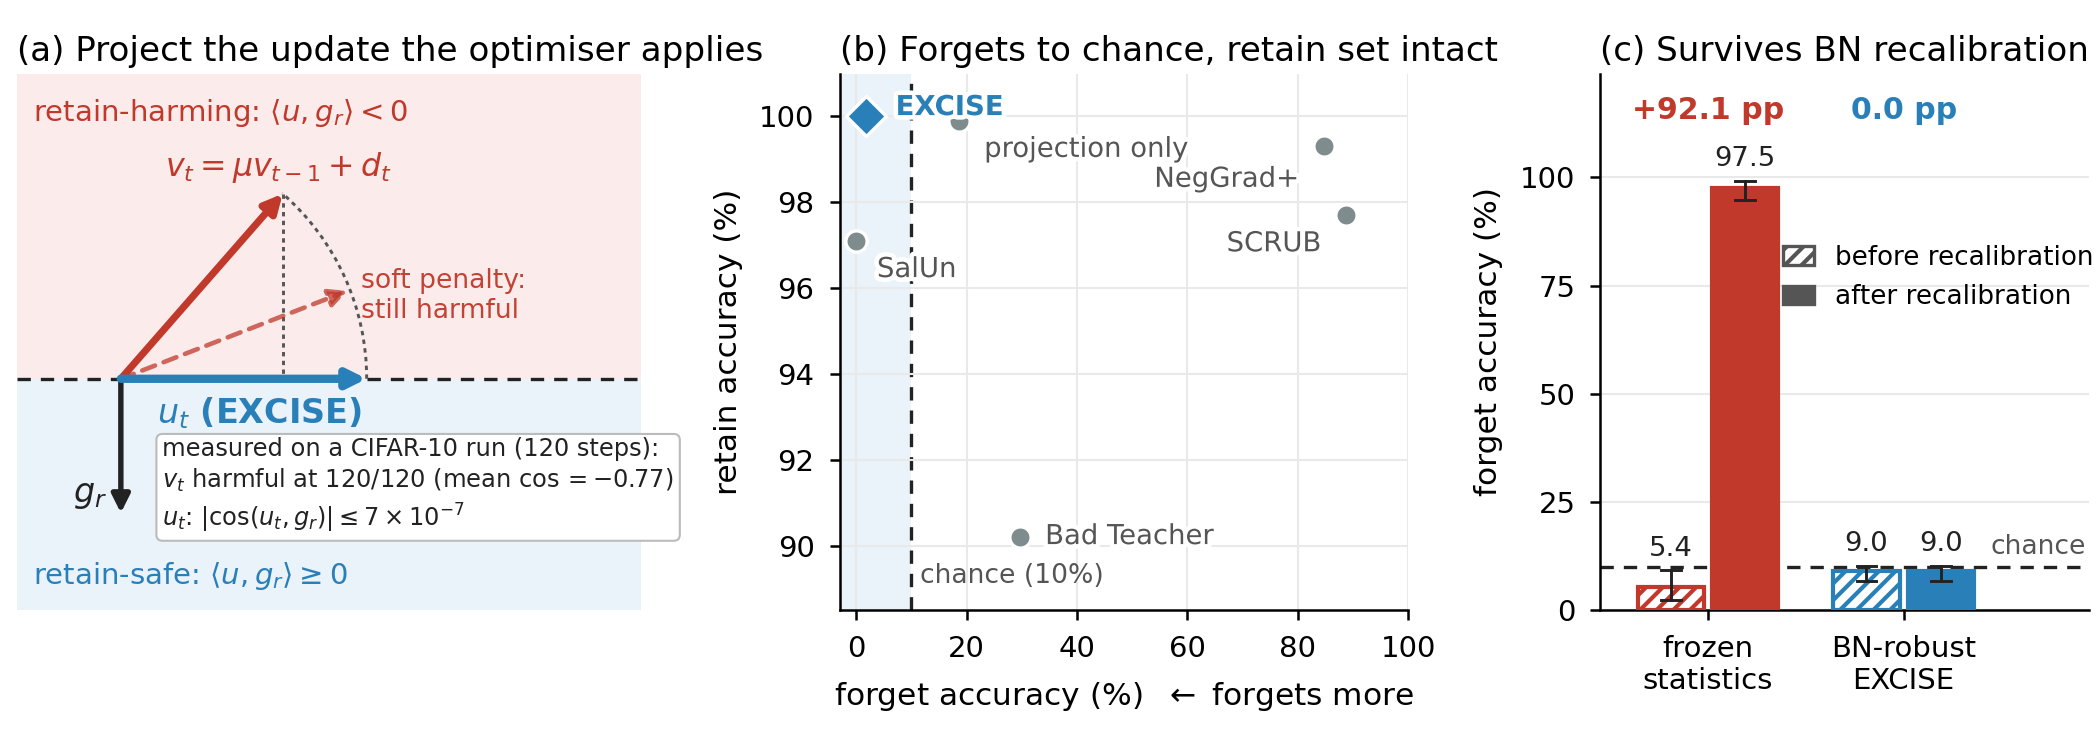
\includegraphics[width=\textwidth]{fig_teaser.png}
\caption{\rev{\textbf{\ours{} in one picture.} \textbf{(a)}~With momentum, the
update the optimiser applies is the accumulated $v_t$, and in unlearning it
points into the retain-harming half-space at every step. \ours{} projects $v_t$
onto the boundary and restores its length, so the applied $u_t$ cannot increase
the sampled retain loss to first order (Theorem~\ref{thm:retain_safety}); a
soft penalty only tilts the step, which stays harmful
(Theorem~\ref{thm:separation}). The boxed numbers are measured
(Figure~\ref{fig:guarantee}). \textbf{(b)}~On CIFAR-10 class~0, \ours{} is the
only method in Table~\ref{tab:cifar10} that forgets to chance with the retain
set intact. \textbf{(c)}~With frozen BatchNorm statistics, recomputing them on
retained data undoes the forgetting on every CIFAR-10 class; BN-robust \ours{}
does not move. Bars are means over the ten classes and whiskers their range
(Table~\ref{tab:app_bnrobust}).}}
\label{fig:teaser}
\end{figure}

\paragraph{The mirror image in continual learning.}
Continual learning (CL) faces the same problem with the sign reversed: learn a
new task while protecting old ones. \rev{One of its most direct answers} is not
a penalty but a \emph{constraint on the update}. A-GEM \citep{chaudhry2019agem} projects any
update $v$ with $\langle v, g_{\text{old}}\rangle < 0$ onto the half-space
$\{u : \langle u, g_{\text{old}}\rangle \ge 0\}$, so a step that would increase
old-task loss to first order is never taken. Unlearning lacks exactly this
guarantee: \rev{most} existing methods control retain damage with weighted
objectives, saliency masks or alternating updates (\S\ref{sec:related}), which
\rev{discourage retain-harming steps rather than exclude them}. We treat the retain set as CL's ``old task'' and
adopt the half-space constraint as the update rule for unlearning. The duality
has been noted before \citep{kurmanji2023unbounded,nguyen2020variational}, and
the forget--retain conflict has been targeted by a soft regulariser
\citep{patel2025learning}\added{ and by projecting updates away from a retain
gradient subspace \citep{hoang2024learn}}; what has not been done\rev{, to our
knowledge,} is to enforce the half-space constraint \rev{against the current
retain gradient}, at every step, on the vector the optimiser applies.

\paragraph{What it takes.}
Three design decisions \rev{complete the method}. \emph{Project the update, not
the gradient}: with momentum, the applied vector is the accumulated update, and
projecting the gradient certifies nothing about it
(Proposition~\ref{prop:counter}). Removing momentum would make the analysis
exact but \rev{leaves forget accuracy far above chance on five of six datasets}
(\S\ref{sec:momentum_ablation}), so we project the post-momentum update and make
the guarantee hold for the optimiser that runs. \emph{Push the forgotten class
toward the model's own retain-confusion distribution}, rather than the uniform
distribution no trained model produces\rev{; at equal test accuracy it forgets
further than gradient ascent and slightly further than a uniform target}
(\S\ref{sec:forget_obj}). \emph{Stop on explicit tolerances} for retain loss and
forget accuracy rather than on an epoch count (\S\ref{sec:stopping}).

\paragraph{Forgetting that survives the attack.}
A fourth issue came from the experiments. Forget batches contain a single
class and would corrupt BatchNorm running statistics, so the method freezes them
during unlearning---and the weights then learn to forget \emph{relative to}
statistics an attacker can replace: recomputing them on retained data restores
forget accuracy from ${\sim}1\%$ to ${\sim}100\%$ without changing a weight
(\S\ref{sec:bn_results}). \rev{The attack reaches beyond us. Concurrent work
\citep{kalani2026batchnorm} applies it to nine prior methods and recovers the
forgotten class for six of them; of the other three, gradient ascent forgets
only by destroying the model ($57\%$ retain accuracy), GA+FT does not forget
($68\%$ forget accuracy), and SCRUB keeps its forgetting at $88\%$ retain
accuracy. Whether a method survives depends less on the method than on how its
statistics are handled during unlearning: in \citet{kalani2026batchnorm},
mixing at least a quarter of retained data into SalUn's unlearning batches
removes its recovery, and our own reproductions of SalUn and Bad Teacher, which
end every epoch with a pass over retained data that recomputes the statistics,
are not recovered at all. BN-robust \ours{} makes survival a property of the
method rather than of how it is run: it keeps the statistics consistent with the
weights throughout unlearning, forgets to chance on every CIFAR-10 class and on
MNIST, survives the attack in every case we tried---including when the attacker
chooses the recalibration data---and keeps the per-step guarantee
(\S\ref{sec:bn_robust}). To our knowledge it is the only unlearning method for
BatchNorm ResNets whose survival has been verified on every class of a benchmark
and against attacker-chosen recalibration data, which we take to make it the
state of the art for this setting, pending a like-for-like run of the prior
methods under the same base and attack (\S\ref{sec:limitations}).}

\paragraph{Contributions.}
\textbf{(1)}~A constrained formulation of class unlearning
(Eq.~\ref{eq:problem}) \rev{that assigns each mechanism of the algorithm to the
condition it enforces}.
\textbf{(2)}~\ours{}: A-GEM projection as the \emph{update rule} of unlearning,
applied to the post-momentum update, with clipping before accumulation and
magnitude-preserving projection. \textbf{(3)}~An exact per-step retain-safety
theorem for that optimiser, a separation theorem showing that gradient ascent,
SCRUB, SalUn and soft conflict penalties admit retain-harming steps, and
\rev{tests of both theorems on real runs}. \textbf{(4)}~\rev{A
BatchNorm-recalibration failure mode of \ours{} and a fix that keeps BatchNorm,
verified on every CIFAR-10 class, on MNIST and against attacker-chosen
recalibration data.} We also show that the conventional MIA target of $0.5$ is
the wrong reference point for class unlearning (\rev{\S\ref{sec:mia_main}}).
\rev{Table~\ref{tab:claims} maps every claim to the experiment that tests it.}

% ============================================================
\section{Related Work}\label{sec:related}

\emph{Exact} unlearning retrains on shards \citep{bourtoule2021sisa} or certifies
removal for convex models \citep{guo2020certified}. \emph{Approximate} methods
modify the trained model: gradient ascent and NegGrad+ \citep{thudi2022unrolling}
maximise forget loss, the latter with a weighted retain term; SalUn
\citep{fan2024salun} confines random-label updates to a saliency mask; Fisher
methods and SSD \citep{golatkar2020eternal,foster2024ssd} dampen parameters by
estimated importance; Bad Teacher \citep{chundawat2023badteacher} and SCRUB
\citep{kurmanji2023unbounded} use distillation, SCRUB alternating forget and
retain steps. Each balances forgetting against retain damage through a weight, a
mask or a schedule, so retain damage is discouraged rather than excluded
(Theorem~\ref{thm:separation}). Closest to us are methods that address the
forget--retain gradient conflict directly: \citet{patel2025learning} with a soft
regulariser that rewards positive alignment, and \added{\citet{hoang2024learn}
by stepping orthogonally to a gradient subspace estimated for the retained
data}. \ours{} instead imposes A-GEM's half-space constraint
\citep{chaudhry2019agem} against the current retain gradient at every step, on
the post-momentum update the optimiser applies, which is what makes its guarantee
exact for the deployed optimiser. Table~\ref{tab:properties} summarises the structural
difference; Appendix~\ref{app:related} gives the full comparison. \rev{On the
evaluation side, \citet{kalani2026batchnorm} show that recomputing BatchNorm
statistics recovers the forgotten class for six of nine prior methods;
\S\ref{sec:bn_results} applies the same attack to \ours{}.}

\begin{table}[t]
\centering
\caption{\textbf{Structural comparison of update rules.} \cmark~= holds by
construction, \pmark~= partial or hyperparameter-dependent, \xmark~= not
provided. Entries are properties of each method's \emph{definition}, not
measured quantities; an empirical comparison against
\citet{patel2025learning} is future work (\S\ref{sec:limitations}).
P\&Q = \citet{patel2025learning}; \rev{PGU = \citet{hoang2024learn}, whose
projection removes the update's component in a retain subspace estimated before
unlearning and truncated at an energy threshold, so its protection is
approximate and not stated against the current retain gradient.}
$^\dagger$\ours{} takes an explicit tolerance and honours it across a $29$pp
range, but only when the stopping rule is evaluated per step: at a 50-batch
check granularity, targets from $5\%$ to $30\%$ collapse onto the same operating
point (\S\ref{sec:further}, Table~\ref{tab:sweeps}).}
\label{tab:properties}
\small
\begin{tabular}{@{}lccccccc@{}}
\toprule
\textbf{Property} & \textbf{GA} & \textbf{SalUn} & \textbf{SCRUB} &
\textbf{NG+} & \textbf{P\&Q} & \rev{\textbf{PGU}} & \textbf{\ours{}} \\
\midrule
Addresses forget--retain gradient conflict & \xmark & \xmark & \pmark & \pmark & \cmark & \cmark & \cmark \\
Conflict handled as a constraint, not a penalty & \xmark & \xmark & \xmark & \xmark & \xmark & \cmark & \cmark \\
Retain-harming steps are unreachable & \xmark & \xmark & \xmark & \xmark & \xmark & \pmark & \cmark \\
Per-step retain-safety guarantee & \xmark & \xmark & \xmark & \xmark & \xmark & \pmark & \cmark \\
Explicit forgetting tolerance & \xmark & \xmark & \pmark & \pmark & \pmark & \pmark & \cmark$^\dagger$ \\
Guarantee holds for the optimiser actually run & \xmark & \xmark & \xmark & \xmark & \xmark & \pmark & \cmark \\
\bottomrule
\end{tabular}
\end{table}

% ============================================================
\section{Problem Formulation}\label{sec:problem}

Let $f_\theta$ be a trained $K$-class classifier with weights $\theta_0$,
$\sigma$ the softmax, and $p_\theta(x) = \sigma(f_\theta(x))$. The training set
splits into a forget set $\Df$ and a retain set $\Dr$. We evaluate with test
accuracy (TA, held-out data), forget accuracy (FA, on $\Df$; a fully unlearned
model reaches at most the chance level $100/K\%$), retain accuracy (RA, on
$\Dr$), and the AUROC of a membership-inference attack (MIA) between forget-class
training and test samples. The \emph{retain-confusion distribution} is the base
model's average prediction on retained data,
\begin{equation}\label{eq:retain_confuse}
p_r = \frac{1}{|\Dr|}\sum_{x \in \Dr} \sigma(f_{\theta_0}(x)),
\end{equation}
and we pose unlearning as \rev{a constrained search: find
\begin{equation}\label{eq:problem}
\theta^\star \in \big\{\theta :\;
\mathrm{FA}(\theta;\Df) \le \tau_F,\;\;
\CE(\theta;\Dr) \le \alpha\,\CE(\theta_0;\Dr),\;\;
\|\theta - \theta_0\| \le R \big\},
\end{equation}
where $\tau_F$ is a forget-accuracy target (the chance level by default),
$\alpha \ge 1$ a tolerance on the retain loss, and $R$ a trust radius. The first
two conditions say what it means to have forgotten without damage; the third
asks for a solution near the trained model, and the search path supplies it.
\ours{} starts at $\theta_0$, descends the forget objective
$\lossf = \mathbb{E}_{x_f}[\KL(p_\theta(x_f)\|p_r)]$ along directions that do
not increase the retain objective
$\lossr = \mathbb{E}_{(x,y)}[\CE(f_\theta(x),y)] + \beta\,\losskd$ to first
order, where $\beta$ weights a distillation anchor, and returns the first point
that meets the forget target. $\lossf$ supplies the direction, not the
destination: driving it to its minimum over-forgets (Appendix~\ref{app:d2r}).
Retain safety is imposed at two levels. At every step the projection of
\S\ref{sec:projection} keeps the applied update in
$\{u : \langle u,\gr\rangle \ge 0\}$, so the sampled retain objective cannot
increase to first order (Theorem~\ref{thm:retain_safety}); on the full retain
set, the stopping rule ends the search if the retain cross-entropy exceeds its
tolerance. The first level is a hard constraint rather than a penalty because a
Lagrangian relaxation would turn it back into the soft treatment whose feasible
set still contains retain-harming steps (Theorem~\ref{thm:separation}(iv)). The
trust region needs no mechanism of its own: every step has length at most
$\eta c/(1-\mu)$ (Theorem~\ref{thm:retain_safety}), so $N$ steps stay within
$R = N\eta c/(1-\mu)$. Table~\ref{tab:constraint_map}
(Appendix~\ref{app:method}) maps each condition to its mechanism.}

% ============================================================
\section{The \ours{} Algorithm}\label{sec:method}

Algorithm~\ref{alg:excise} gives the update. Each step computes a retain gradient
$\gr$ on a retain mini-batch (cross-entropy plus the distillation anchor) and a
forget gradient $\gf$ on a forget mini-batch.

\begin{algorithm}[t]
\caption{\ours{} unlearning (projected-momentum update)}\label{alg:excise}
\begin{algorithmic}[1]
\REQUIRE Trained model $\theta$, forget set $\Df$, retain set $\Dr$;
         lr $\eta$, momentum $\mu$, clip $c$, weight decay $\lambda_{\mathrm{wd}}$;
         \rev{targets $\tau_F$, $\alpha$; check interval $m$}
\ENSURE Unlearned model $\theta^*$
\STATE $\theta_{\text{orig}} \leftarrow \text{freeze}(\text{copy}(\theta))$;\quad
       set all BatchNorm layers to \texttt{eval} mode
\STATE $p_r \leftarrow \frac{1}{|\Dr|}\sum_{x \in \Dr}\sigma(\theta_{\text{orig}}(x))$
\STATE $L_0 \leftarrow \CE(\theta,\Dr)$;\quad $v \leftarrow 0$
\FOR{epoch $=1$ to $T$}
  \FOR{$(x_f,y_f)$ in $\Df$}
    \STATE Sample $(x_r,y_r)$ from $\Dr$
    \STATE $\gr \leftarrow \nabla_\theta[\CE(f_\theta(x_r),y_r) + \beta\losskd]$
    \STATE $\gf \leftarrow \nabla_\theta\lossf(\theta;x_f)$
    \STATE $d \leftarrow \mathrm{clip}_c\!\big(\gf + \lambda_{\mathrm{wd}}\theta\big)$
           \hfill\textit{// clip BEFORE accumulation}
    \STATE $v \leftarrow \mu v + d$
           \hfill\textit{// momentum}
    \IF{$\langle v, \gr\rangle < 0$}
      \STATE $u \leftarrow v - \frac{\langle v,\gr\rangle}{\|\gr\|^2}\gr$;\quad
             $u \leftarrow u\,\|v\|/\|u\|$
             \hfill\textit{// project the update, rescale}
    \ELSE
      \STATE $u \leftarrow v$
    \ENDIF
    \STATE $\theta \leftarrow \theta - \eta u$
    \IF{\rev{every $m$ steps:} $\mathrm{FA}(\theta,\Df) \le \tau_F$}
      \STATE \textbf{return} $\theta$ \hfill\textit{\rev{// forget target met}}
    \ENDIF
  \ENDFOR
  \IF{$\CE(\theta,\Dr) > \alpha L_0$}
    \STATE \textbf{return} $\theta$ \hfill\textit{\rev{// retain tolerance exceeded}}
  \ENDIF
\ENDFOR
\RETURN $\theta^* \leftarrow \theta$
\end{algorithmic}
\end{algorithm}

\subsection{Projection onto the Retain-Safe Half-Space}\label{sec:projection}

When a candidate update $v$ satisfies $\langle v,\gr\rangle < 0$, moving along it
would increase the retain loss to first order, and we replace it by its
projection
\begin{equation}\label{eq:projection}
\Pi_{\gr}(v) = v - \frac{\langle v,\gr\rangle}{\|\gr\|^2}\,\gr,
\qquad \langle \Pi_{\gr}(v),\gr\rangle = 0 .
\end{equation}
This is A-GEM's operator: the minimum-norm correction that restores
feasibility, at the cost of one extra backward pass. What changes is its role.
In A-GEM it occasionally corrects a process whose objective already points the
right way; in unlearning, erasing a class and keeping the rest are directly
opposed, and the projection fires at \rev{$96$--$100\%$ of steps in every \ours{}
run we logged} (\S\ref{sec:guarantee_measured}). It becomes the optimiser's defining step rather
than a safeguard, which has three consequences for how it must be applied.

\subsection{Which Vector to Project}\label{sec:optimiser}

\emph{(i) Project the update, not the gradient.} \ours{} uses SGD with momentum
$\mu$, weight decay and clipping $c$. The vector applied to the weights is the
accumulated update, so we accumulate first and project afterwards
(Algorithm~\ref{alg:excise}, lines 10--15); projecting $\gf$ instead leaves the
applied update unconstrained (Proposition~\ref{prop:counter},
Figure~\ref{fig:projorder}). \emph{(ii) Clip before accumulating.} Clipping the
per-step ingredient keeps momentum's $1/(1-\mu)$ amplification and gives
$\|v_t\| \le c/(1-\mu)$; clipping the final update would cap it at $c$\rev{,
the step size of the momentum-free update, which leaves forget accuracy far
above chance on five of six datasets (\S\ref{sec:momentum_ablation},
Proposition~\ref{prop:clip}). Raw forget gradients are ${\sim}100\times$ the
clip threshold, so clipping is always active and that cap would always bind.}
\emph{(iii) Preserve magnitude.} Projection shrinks the update by
$\sin\vartheta$, which vanishes when forget and retain gradients are nearly
opposed \rev{(on the logged CIFAR-10 run it falls to $0.37$)}, so we rescale the
projected update to the pre-projection norm; $\langle u_t,\gr\rangle = 0$ is
unaffected.

\begin{figure}[t]
\centering
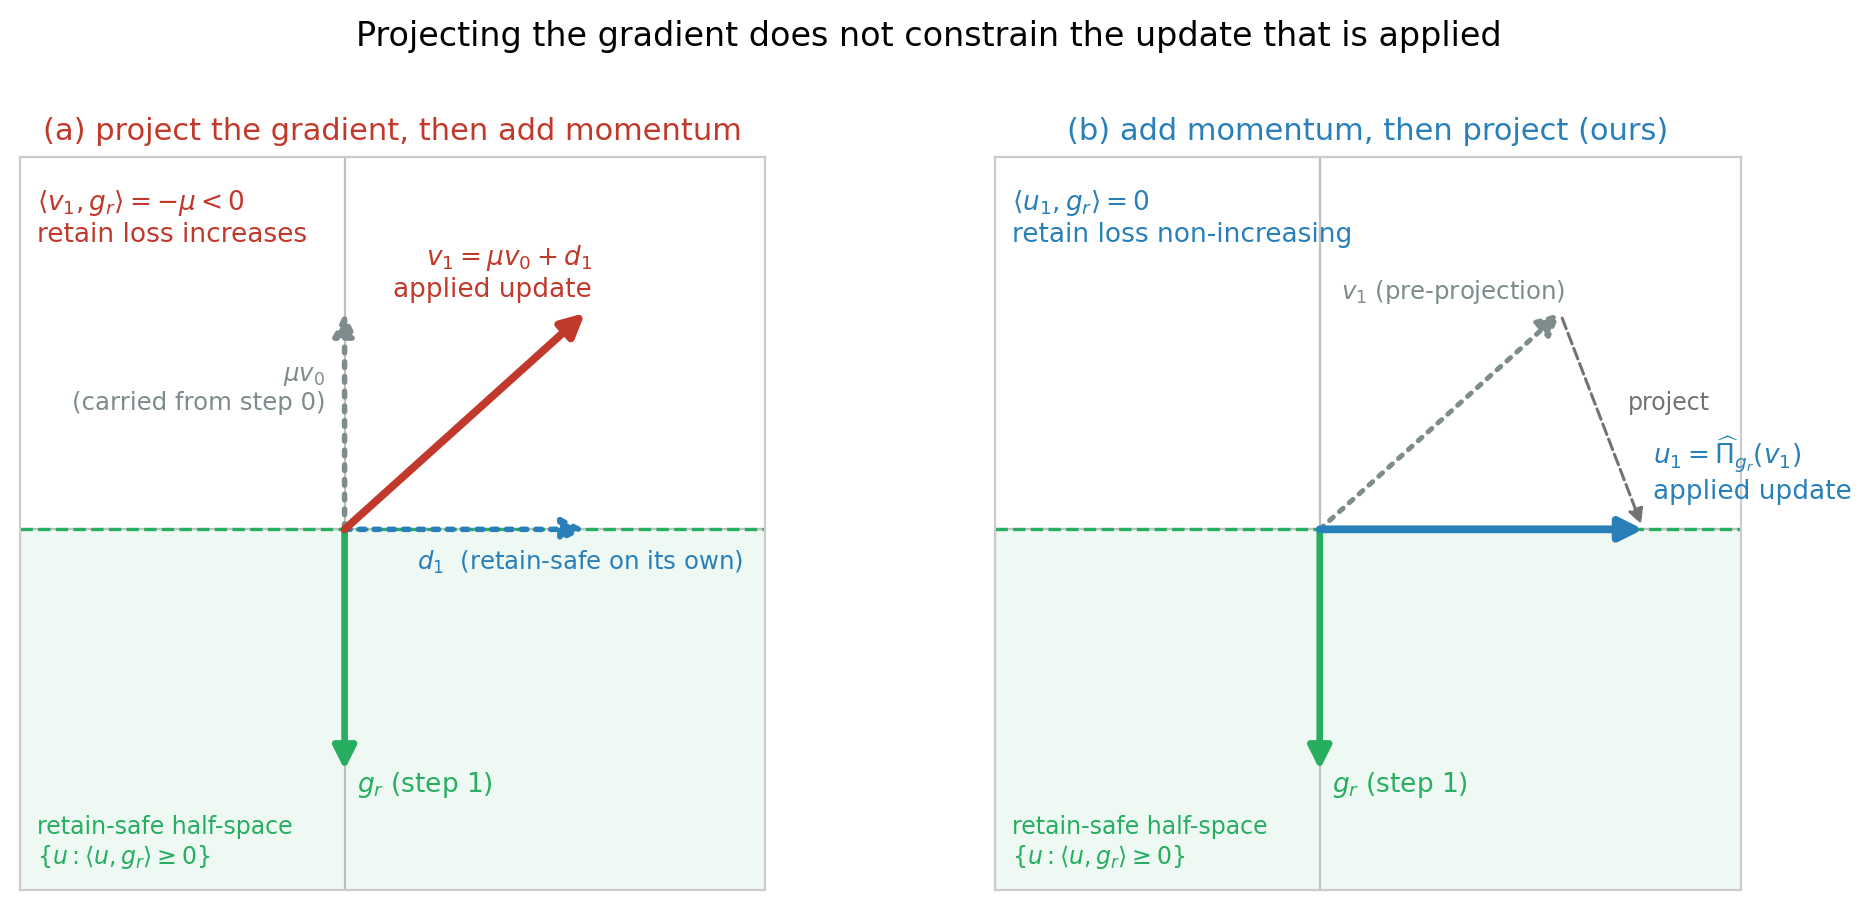
\includegraphics[width=0.86\textwidth]{fig_projection_order.png}
\caption{\textbf{Why the projection is applied to the update, not the
gradient} (Proposition~\ref{prop:counter}). Both panels show step~1, whose
constraint is $\gr$; the retain-safe half-space is shaded. \textbf{(a)}~Each
ingredient is individually retain-safe---$d_1$ lies on the boundary, and
$\mu v_0$ was certified against step~0's constraint---yet their sum, the vector
actually applied, lies in the harming half-space with
$\langle v_1,\gr\rangle = -\mu$. The violation grows with $\mu$.
\textbf{(b)}~Projecting the accumulated update instead returns it to the
boundary, so the certificate is issued against the constraint in force where
the step is taken.}
\label{fig:projorder}
\end{figure}

\subsection{Forget Objective, Stopping, and Normalisation}\label{sec:forget_obj}

The \klr{} objective drives forget-set predictions toward the retain-confusion
distribution rather than the uniform one,
\begin{equation}\label{eq:kl_retain}
\mathcal{L}_{\text{KL-R}} = \KL\!\left(\log\sigma(f_\theta(x_f)) \,\|\, p_r\right).
\end{equation}
Under the projected-momentum optimiser it forgets further than gradient ascent
\rev{and slightly further than a uniform target at equal test accuracy (FA
$2.1\%$ against $8.2\%$ and $3.9\%$, at TA $86.1$, $86.4$ and $86.4\%$; CIFAR-10
class~0, one seed)} and is within noise of a uniform target on MIA, so we claim a
better forget \emph{direction}, not a closer imitation of a retrained model
(Appendix~\ref{app:method}).

\paragraph{Dual stopping.}\label{sec:stopping}
Unlearning halts if the retain \rev{cross-entropy, measured on the full retain
set after each epoch,} exceeds $\alpha$ times its initial value, and completes
when FA reaches \rev{the target $\tau_F$}---by default the chance level
$100/K\%$---checked \rev{every $m=50$ steps} within epochs, because FA can fall
by tens of points inside one.

\paragraph{BatchNorm.}\label{sec:bn}
Class-homogeneous forget batches would corrupt BatchNorm running statistics, so
\ours{} freezes them. \added{The weights then learn to forget relative to those
frozen statistics; \S\ref{sec:bn_results} shows that this forgetting does not
survive recomputing them, and BN-robust \ours{} recomputes them from retained
data before every step instead (\S\ref{sec:bn_robust}).} A distillation anchor to
the frozen base model \rev{enters the retain objective; removing it changes
retain accuracy by only $0.04$pp on CIFAR-10 (\S\ref{sec:guarantee_measured}),
so we keep it as a safeguard rather than claim it as load-bearing}.

% ============================================================
\section{Theoretical Guarantees}\label{sec:theory}

\begin{theorem}[Exact per-step retain safety under momentum]\label{thm:retain_safety}
Let \rev{$\Lrt$, the retain objective $\lossr$ (cross-entropy plus
$\beta\losskd$) evaluated on the sampled retain mini-batch,} be $L$-smooth, and
let $\gr = \nabla_\theta\Lrt(\theta_t)$. Let \ours{} run the update of
Algorithm~\ref{alg:excise}: $\|d_t\| \le c$ by clipping,
$v_t = \mu v_{t-1} + d_t$ with $v_{-1}=0$ and $\mu \in [0,1)$,
$u_t = \Pi_{\gr}(v_t)\,\|v_t\|/\|\Pi_{\gr}(v_t)\|$ when
$\langle v_t,\gr\rangle<0$ \rev{(and $u_t=0$ if $\Pi_{\gr}(v_t)=0$)} and
$u_t = v_t$ otherwise, and $\theta_{t+1} = \theta_t - \eta u_t$. Then, exactly
and \rev{with no assumption on $\gf$ or on its alignment with $\gr$},
\begin{equation}\label{eq:thm1}
\langle u_t,\gr\rangle \ge 0,
\qquad \|u_t\| \;\rev{\le}\; \|v_t\| \;\le\; \frac{c}{1-\mu},
\qquad \Lrt(\theta_{t+1}) \;\le\; \Lrt(\theta_t) + \tfrac{1}{2}L\eta^2\Big(\frac{c}{1-\mu}\Big)^{\!2}.
\end{equation}
\end{theorem}

\begin{proof}[Proof sketch]
The first claim is immediate: if $\langle v_t,\gr\rangle \ge 0$ then $u_t=v_t$;
otherwise $\langle \Pi_{\gr}(v_t),\gr\rangle = 0$ identically, and rescaling by
a positive scalar preserves this. For the second, $\Pi_{\gr}$ is the orthogonal
projection onto $\{u : \langle u,\gr\rangle = 0\}$, so the rescaling restores
$\|u_t\|=\|v_t\|$ \rev{unless the projection vanishes}; unrolling the buffer gives
$v_t = \sum_{k=0}^{t}\mu^{t-k}d_k$, hence
$\|v_t\| \le c\sum_{j=0}^{t}\mu^{j} < c/(1-\mu)$. The third follows from
$L$-smoothness,
$\Lrt(\theta_{t+1}) \le \Lrt(\theta_t) - \eta\langle u_t,\gr\rangle
+ \tfrac{1}{2}L\eta^2\|u_t\|^2$, where the first-order term is non-positive by
claim one and $\|u_t\|$ is bounded by claim two. The full proof, together with the three supporting lemmas, is given in Appendix~\ref{app:thm1} (Theorem~\ref{thm:app_main}).
\end{proof}

The first-order change in the sampled retain loss is non-positive at every step,
and, unlike guarantees stated for momentum-free surrogates, the analysed $u_t$ is
the vector the code applies. The bound concerns the sampled mini-batch objective,
not the population retain loss (\S\ref{sec:limitations}).
\rev{Section~\ref{sec:guarantee_measured} tests the theorem on a logged run.}

\begin{theorem}[Per-step separation]\label{thm:separation}
For any model $\theta_0$ with retain gradient $\gr$:
\textbf{(i)}~GA's update $+\eta\gf$ strictly increases retain loss to first
order whenever $\langle\gf,\gr\rangle>0$;
\textbf{(ii)}~SCRUB's $-\gf+\lambda\gr$ can have $\langle\cdot,\gr\rangle<0$ for
any fixed $\lambda$;
\textbf{(iii)}~SalUn's masked random-label gradient has unconstrained sign with
respect to $\gr$;
\textbf{(iv)}~a soft conflict regulariser that adds $\rho\,\phi(\langle
g,\gr\rangle)$ with $\phi$ decreasing---the approach of the closest prior work
\citep{patel2025learning}---shifts the optimum toward positive alignment but
leaves the feasible set unrestricted: for any finite $\rho$, a sufficiently
large forget-loss reduction still makes a step with $\langle g,\gr\rangle<0$
preferable.
\rev{Among these update rules, only \ours{}'s} guarantees
$\langle u_t,\gr\rangle \ge 0$ \rev{at every step}, because only a projection
makes such steps unreachable rather than merely costly.
\end{theorem}

% ============================================================
\section{Experiments}\label{sec:experiments}

\subsection{Setup}\label{sec:setup}

We forget one class at a time on six benchmarks that vary class count, examples
per class and domain: CIFAR-10 and CIFAR-100 \citep{krizhevsky2009cifar}, MNIST
\citep{lecun1998mnist}, SVHN \citep{netzer2011svhn}, STL-10
\citep{coates2011stl10} and PathMNIST \citep{yang2023medmnist}. We forget every
class of MNIST and PathMNIST, \rev{classes $10, 20, \dots, 90$ of CIFAR-100}, and
class~0 of CIFAR-10, SVHN and STL-10 over three seeds: 31 tasks and 75 runs. All
models are ResNet-18 \citep{he2016resnet}. \rev{SalUn, SCRUB, Bad Teacher and
NegGrad+ are re-run on our stack, and a model retrained without the forget class
serves as the reference. MIA is the mean AUROC of a loss and a confidence
attack.} Hyperparameters are fixed per dataset and released as configuration
files (Appendix~\ref{app:hyper}); Appendix~\ref{app:experiments} gives the full
protocol. \rev{Table~\ref{tab:claims} lists every claim of \S\ref{sec:intro}
with the experiment that tests it; the subsections follow its order.}

\begin{table}[t]
\centering\color{revisedB}
\caption{\rev{\textbf{Each claim and the experiment that tests it.}}}
\label{tab:claims}
\small
\renewcommand{\arraystretch}{1.08}
\begin{tabular}{@{}>{\raggedright\arraybackslash}p{0.28\textwidth}>{\raggedright\arraybackslash}p{0.26\textwidth}>{\raggedright\arraybackslash}p{0.40\textwidth}@{}}
\toprule
\textbf{Claim} & \textbf{Test} & \textbf{Outcome} \\
\midrule
Forgets to chance, retain set intact & 31 tasks, six datasets (Table~\ref{tab:cross}) & Chance on all six, two at 60 epochs; RA $\ge 97.2\%$ on the 10-class datasets \\
Only \ours{} does both on CIFAR-10 & Four baselines, projection only (Table~\ref{tab:cifar10}) & FA $1.87\%$ at RA $100\%$; SalUn loses $2.9$pp RA, the rest stop at FA $\ge 18.7\%$ \\
Theorem~\ref{thm:retain_safety} holds for the optimiser that runs & Step-level audit (Figure~\ref{fig:guarantee}) & $120/120$ steps conflict before projection; $|\cos| \le 7.4\times10^{-7}$ after; $\|u_t\| \le 9.16 < 10$ \\
Soft corrections leave harm reachable (Thm.~\ref{thm:separation}) & Projection strength $s$, equal compute (\S\ref{sec:guarantee_measured}) & RA rises from $52.5$ to $99.98\%$ as $s \to 1$; every $s<1$ leaves conflict in the applied step \\
The projection protects the retain set & Ablation, equal compute (\S\ref{sec:guarantee_measured}) & Without it RA is $52.6\%$; alone it keeps RA $99.9\%$ but stops at FA $18.7\%$ \\
The guarantee must cover momentum & $\mu = 0$ ablation (Table~\ref{tab:momentum}) & With $\mu=0$, FA stays far above chance on five of six datasets \\
Frozen statistics make forgetting reversible & Recalibration attack (Table~\ref{tab:bnrecal}) & Frozen \ours{}: FA $1.4 \to 99.7\%$; base model and our baselines: $\Delta F \le 0$ \\
BN-robust \ours{} survives it & Ten classes, MNIST, attacker's data (Figures~\ref{fig:teaser}c, \ref{fig:bnrobust_attack}) & $|\Delta F| \le 0.06$pp on every CIFAR-10 class, $+0.09$pp on MNIST; attacker's data: $-1.2$ to $-1.0$pp \\
$0.5$ is the wrong MIA target & Retrained references (Table~\ref{tab:mia_main}) & References score $0.69$ (CIFAR-10) and $0.31$--$0.70$ (PathMNIST); rankings reverse \\
$p_r$ is a better direction than uniform & Forget objectives, equal TA (\S\ref{sec:forget_obj}) & FA $2.1\%$ against $3.9\%$ (uniform) and $8.2\%$ (GA); one seed \\
\bottomrule
\end{tabular}
\end{table}

\subsection{Main Results}\label{sec:main_results}

\begin{table}[t]
\centering
\caption{\textbf{Cross-dataset results.} Mean $\pm$ \rev{sample} std over
classes $\times$ seeds (3 seeds \rev{per task; one seed per class for
CIFAR-100}). \#T = number of forgetting tasks. Chance $=100/K\%$ is the level a
fully unlearned model must reach. \rev{The upper block uses each dataset's epoch
cap (12--20 epochs, Appendix~\ref{app:hyper}), which penalises datasets with few
images per class, since the binding resource is optimiser steps rather than
epochs. The lower block re-runs the two datasets that fall short at 60 epochs
($4\times$ and $3\times$ their caps), with a per-step check and a $1\%$ forget
target,} on the same seeds and classes;
$^*$marks the STL-10 row it supersedes (\S\ref{sec:crossdataset_stl}).}
\label{tab:cross}
\begin{tabular}{@{}lccccccc@{}}
\toprule
\textbf{Dataset} & \textbf{\#T} & \textbf{Chance} & \textbf{TA} & \textbf{FA}$\downarrow$ & \textbf{RA} & \textbf{MIA} \\
\midrule
CIFAR-10    & 1 & 10.0\% & $86.13 \pm 0.02$ & $\mathbf{1.87} \pm 0.25$ & $100.00 \pm 0.00$ & $0.529 \pm 0.001$ \\
MNIST       & 10 & 10.0\% & $90.00 \pm 0.64$ & $\mathbf{6.17} \pm 2.81$ & $99.49 \pm 0.04$ & $0.497 \pm 0.009$ \\
SVHN        & 1 & 10.0\% & $89.69 \pm 0.02$ & $\mathbf{5.75} \pm 0.17$ & $97.26 \pm 0.01$ & $0.525 \pm 0.001$ \\
STL-10$^*$  & 1 & 10.0\% & $92.84 \pm 0.02$ & $75.67 \pm 1.70$ & $99.38 \pm 0.10$ & $0.466 \pm 0.005$ \\
PathMNIST   & 9 & 11.1\% & $80.96 \pm 5.39$ & $\mathbf{5.82} \pm 3.42$ & $98.88 \pm 0.31$ & $0.483 \pm 0.084$ \\
CIFAR-100   & 9 & \phantom{0}1.0\% & $76.17 \pm 0.86$ & $4.07 \pm 5.51$ & $92.19 \pm 0.84$ & $0.500 \pm 0.037$ \\
\midrule
\multicolumn{7}{@{}l}{\emph{Extended budget} (\rev{60 epochs, per-step check, $1\%$ forget target}; same seeds and classes)} \\
STL-10      & 1 & 10.0\% & $85.15 \pm \rev{0.06}$ & $\mathbf{1.73} \pm \rev{0.95}$ & $98.87 \pm \rev{0.05}$ & $\rev{0.488} \pm \rev{0.008}$ \\
CIFAR-100   & 9 & \phantom{0}1.0\% & $75.50 \pm \rev{0.68}$ & $\mathbf{1.27} \pm \rev{0.39}$ & $91.32 \pm \rev{0.94}$ & $\rev{0.490} \pm \rev{0.043}$ \\
\bottomrule
\end{tabular}
\end{table}

\begin{table}[t]
\centering
\caption{\textbf{CIFAR-10 class-0 forgetting.} \ours{} is a 3-seed mean $\pm$
std. Methods with FA~$>80\%$ attain MIA~$\approx 0.5$ trivially, by barely
changing the model. $\dagger$Our reproduction; $\ddagger$our reproduction with
unified MIA. $^\S$A-GEM projection applied to plain gradient ascent, with
\ours{}'s KD anchor and retain-confusion target removed: the direct
projected-gradient baseline, isolating what the projection alone achieves.
\rev{$^\P$The retrained reference of \S\ref{sec:mia_main}; its TA and RA were
not logged, and its MIA, from the same two attacks, is $0.565$, not $0.5$.}}
\label{tab:cifar10}
\begin{tabular}{@{}lcccc@{}}
\toprule
\textbf{Method} & \textbf{TA} & \textbf{FA}$\downarrow$ & \textbf{RA} & \textbf{MIA} \\
\midrule
\rev{Retrain (reference)$^\P$} & \rev{---} & 0.0 & \rev{---} & \rev{0.565} \\
\midrule
SalUn$^\dagger$        & 84.0 & 0.0  & 97.1 & 0.497 \\
Bad Teacher$^\ddagger$ & 82.0 & 29.7 & 90.2 & 0.499 \\
SCRUB$^\ddagger$       & 93.3 & 88.8 & 97.7 & 0.515 \\
NegGrad+$^\ddagger$    & 94.2 & 84.8 & 99.3 & 0.525 \\
\midrule
Projection-only$^\S$   & 86.23 & 18.66 & 99.90 & 0.511 \\
\midrule
\textbf{\ours{}} & $\mathbf{86.13}\pm.02$ & $\mathbf{1.87}\pm.25$ & $\mathbf{100.00}\pm.00$ & $\mathbf{0.529}\pm.001$ \\
\bottomrule
\end{tabular}
\end{table}

\rev{At its epoch cap} \ours{} drives FA to or below the chance level on four
of six datasets with RA $\ge 97.2\%$ (CIFAR-100: $92.2\%$), and \rev{the mean
over seeds is below chance for every one of the ten MNIST and nine PathMNIST
classes (one of the 30 MNIST runs ends at $10.2\%$, within sampling error)}
(Table~\ref{tab:cross}, Appendix~\ref{app:perclass}). The two shortfalls are
budget-limited: STL-10 gets ${\sim}60$ optimiser steps at \rev{its 15-epoch cap}
against ${\sim}600$ for CIFAR-10 \rev{at the same cap}, and at 60 epochs
\rev{(per-step check, $1\%$ target)} STL-10 reaches $1.73\%$ \rev{($9.2\%$ in a
single run at its default $10\%$ target)} and CIFAR-100 $1.27\%$\rev{---against a $1\%$ chance level,
within one standard error of a 500-image forget set}---so all six datasets reach
chance. On CIFAR-10 (Table~\ref{tab:cifar10}, \rev{Figure~\ref{fig:teaser}b}),
\ours{} is the only method \rev{in the table} that both forgets to chance
and leaves retain accuracy untouched: SalUn forgets fully but costs $2.9$pp of
retain accuracy, Bad Teacher stops at $29.7\%$ while damaging the model, and
SCRUB and NegGrad+ keep the model intact by barely forgetting. The projection
alone does not unlearn: applied to plain gradient ascent it preserves the retain
set but stalls at $18.66\%$, so the projection supplies retain safety and the
\klr{} objective supplies the forgetting.

\subsection{The Guarantees, Measured}\label{sec:guarantee_measured}

\begin{figure}[t]
\centering
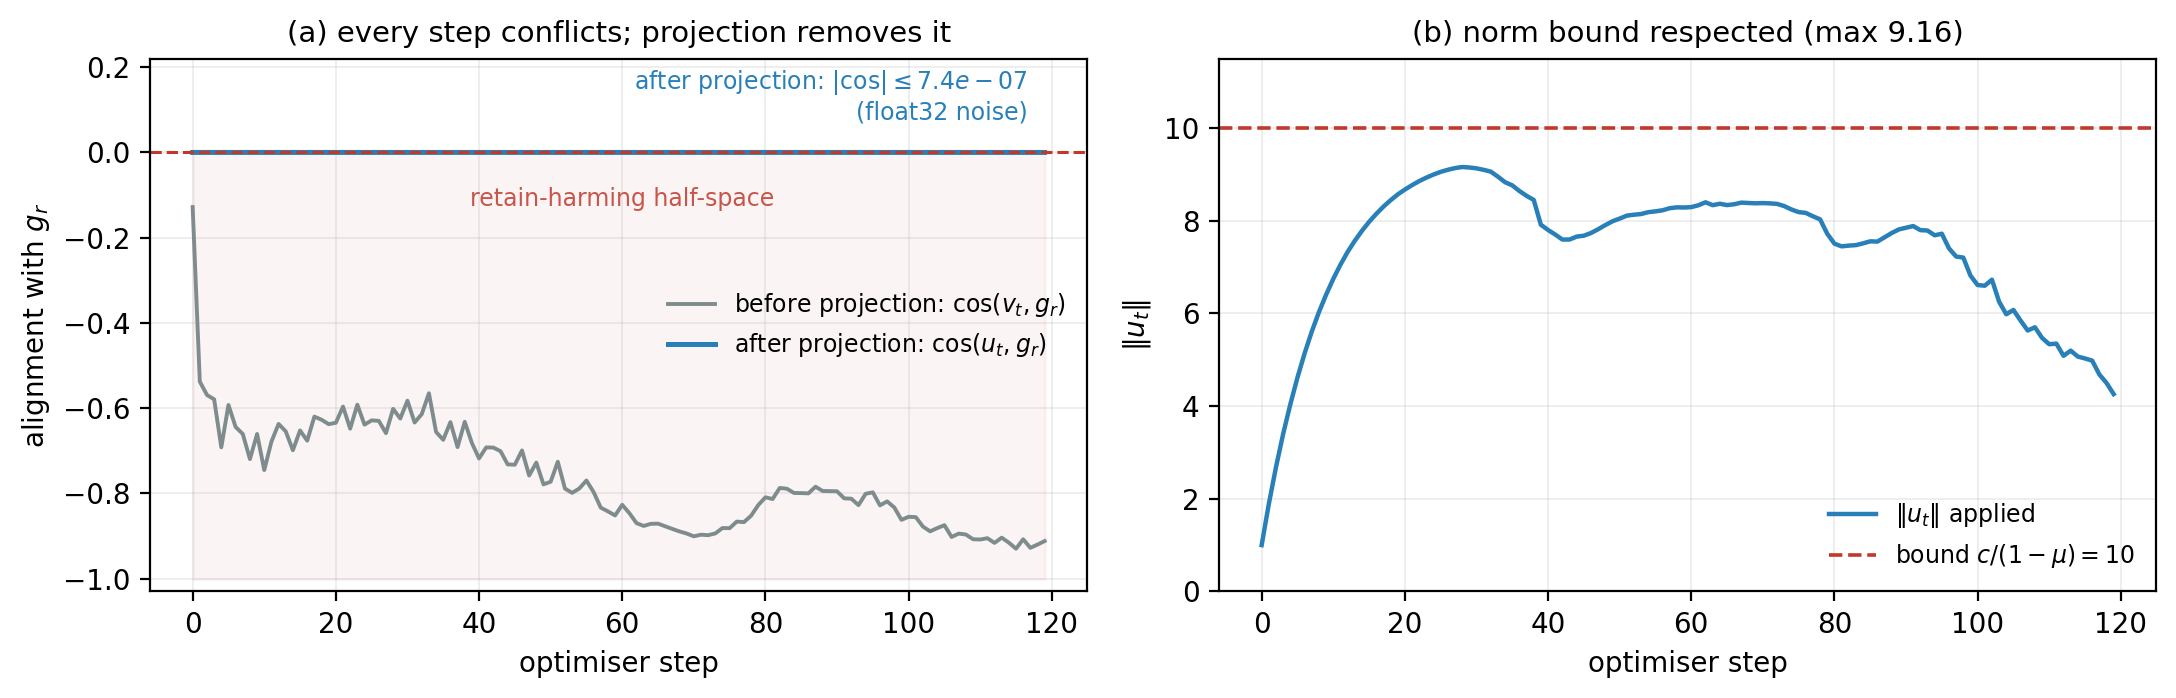
\includegraphics[width=0.86\textwidth]{fig_guarantee.png}
\caption{\textbf{Theorem~\ref{thm:retain_safety} audited on a real run}
(CIFAR-10 class~0, 120 steps). \textbf{(a)}~Alignment with the retain gradient,
normalised to $\cos(\cdot,\gr)$. Before projection every step lies in the
retain-harming half-space (mean $-0.77$); after projection the alignment is
indistinguishable from zero ($|\cos| \le 7.4\times10^{-7}$, the float32
accumulation scale). \textbf{(b)}~The applied update never exceeds the bound
$c/(1-\mu)=10$ of Eq.~\ref{eq:thm1}, peaking at $9.16$---tight, but respected.}
\label{fig:guarantee}
\end{figure}

\rev{\paragraph{Theorem~\ref{thm:retain_safety} on a real run.}
We log every step of a CIFAR-10 run (class~0, 120 steps;
Figure~\ref{fig:guarantee}, Appendix~\ref{sec:alignment}). The accumulated update
conflicts with the retain gradient at all 120 steps (mean
$\cos(v_t,\gr) = -0.77$), so the projection is the optimiser's defining step
rather than a safeguard. After projection the alignment is zero to float32
precision ($|\cos(u_t,\gr)| \le 7.4\times10^{-7}$), and $\|u_t\|$ peaks at
$9.16$ against the bound $c/(1-\mu)=10$.

\paragraph{Theorem~\ref{thm:separation}(iv): soft against hard.}
To test the separation without reimplementing another method, we vary our own
projection between a soft correction and the hard constraint: at conflicting
steps $u = v - s\,\frac{\langle v,\gr\rangle}{\|\gr\|^2}\gr$, so
$\langle u,\gr\rangle = (1-s)\langle v,\gr\rangle < 0$ for every $s<1$. At equal
compute with stopping disabled every setting forgets completely (FA $0.0\%$), so
the settings differ only in collateral damage: RA is $52.5$, $81.4$, $92.8$,
$98.2$ and $99.98\%$ for $s = 0, 0.25, 0.5, 0.75, 1$ (Appendix~\ref{sec:strength}).
The curve is gradual---$s=0.75$ already keeps $98.2\%$---so the case for $s=1$
is that it is the only setting with a guarantee, not that the last $1.8$pp is
large.

\paragraph{The projection is what protects the retain set.}
At equal compute with stopping disabled, removing the projection collapses the
model (TA $44.4\%$ and RA $52.6\%$, against $85.7\%$ and $99.98\%$ with it),
removing the distillation anchor changes RA by $0.04$pp, and the projection on
its own keeps RA at $99.9\%$ but stalls at FA $18.7\%$
(Tables~\ref{tab:cifar10} and~\ref{tab:ablation}). With stopping enabled every
variant halts after one epoch and the projection looks costless, which is why we
report both modes.}

\subsection{Momentum Is Not Incidental}\label{sec:momentum_ablation}

\begin{table}[t]
\centering
\caption{\textbf{Momentum ablation.} Removing momentum to simplify the analysis
\rev{leaves forget accuracy far above chance on five of six datasets; on STL-10
projected momentum also falls short at this budget (Table~\ref{tab:cross})}.
High RA with high FA indicates the model barely changed. Same configs, seeds,
and stopping rules throughout.}
\label{tab:momentum}
\begin{tabular}{@{}lccccc@{}}
\toprule
& & \multicolumn{2}{c}{$\mu=0$ (analysis-friendly)} & \multicolumn{2}{c}{Projected momentum (ours)} \\
\cmidrule(lr){3-4}\cmidrule(lr){5-6}
\textbf{Dataset} & \textbf{Chance} & \textbf{FA}$\downarrow$ & \textbf{RA} & \textbf{FA}$\downarrow$ & \textbf{RA} \\
\midrule
CIFAR-10  & 10.0\% & \phantom{0}5.8 & 100.0 & \phantom{0}1.9 & 100.0 \\
MNIST     & 10.0\% & 95.9 & \phantom{0}99.5 & \phantom{0}6.2 & 99.5 \\
SVHN      & 10.0\% & 61.9 & \phantom{0}97.4 & \phantom{0}5.8 & 97.3 \\
STL-10    & 10.0\% & 99.7 & \phantom{0}99.4 & 75.7 & 99.4 \\
PathMNIST & 11.1\% & 16.4 & \phantom{0}99.0 & \phantom{0}5.8 & 98.9 \\
CIFAR-100 & \phantom{0}1.0\% & 73.7 & \phantom{0}94.1 & \phantom{0}4.1 & 92.2 \\
\bottomrule
\end{tabular}
\end{table}

Removing momentum is the most direct route to an exact guarantee, since the
applied update then equals the projected gradient. Table~\ref{tab:momentum} shows
the cost: with $\mu = 0$ and everything else fixed, \rev{forget accuracy stays
far above chance on five of six datasets} (FA $95.9\%$ on MNIST, $99.7\%$ on
STL-10, $73.7\%$ on CIFAR-100), and RA stays high only because the model barely
moves. \rev{STL-10 does not forget at this budget with momentum either
($75.7\%$), so the comparison rests on the other four: without momentum all four
stay far above chance; with it, three reach chance and CIFAR-100 ends at
$4.1\%$.} A guarantee stated for the momentum-free update would be exact and
would describe a method that does not unlearn. The dependence is not ours alone:
every update rule we tested loses forgetting without momentum, but the KL
objectives lose $70$--$79$pp against $12$--$15$pp for gradient ascent \rev{(with
or without projection; means over MNIST and SVHN), consistent with a bounded
objective needing} momentum's $1/(1-\mu)$ amplification
(Appendix~\ref{app:momentum}).

\subsection{BatchNorm: the Attack, and a Fix That Keeps BatchNorm}\label{sec:bn_results}

\begin{table}[t]
\centering
\caption{\textbf{BatchNorm recalibration} (CIFAR-10, class~0), using
\texttt{update\_bn} on the retain set: BatchNorm buffers are reset and
recomputed, no weight is touched. \rev{Our reproductions of the baselines}
and the un-unlearned base model are unaffected ($\Delta F \le 0$); \ours{} with a
BatchNorm backbone loses essentially all of its forgetting. The two backbones without running statistics
are outside the operator's reach by construction. NegGrad+ is omitted: no
checkpoint for it was available.}
\label{tab:bnrecal}
\begin{tabular}{@{}lccccc@{}}
\toprule
Configuration & pre-$F$ & post-$F$ & $\boldsymbol{\Delta F}$ & pre-TA & post-TA \\
\midrule
Base model (no unlearning)  & $100.0$ & $99.8$ & $-0.2$ & $95.5$ & $92.9$ \\
SalUn                       & $0.0$   & $0.0$  & $+0.0$ & $84.7$ & $84.4$ \\
Bad Teacher                 & $28.7$  & $28.4$ & $-0.3$ & $81.5$ & $84.0$ \\
SCRUB                       & $89.3$  & $85.7$ & $-3.6$ & $93.5$ & $93.2$ \\
\midrule
\ours{} (BatchNorm, frozen) & $1.4$   & $99.7$ & $\mathbf{+98.4}$ & $86.1$ & $92.9$ \\
\ours{} (GroupNorm)         & $4.9$   & $4.9$  & $\mathbf{0.0}$   & $84.2$ & $84.2$ \\
\ours{} (ViT-B/16, LayerNorm) & $9.6$ & $9.6$  & $\mathbf{0.0}$   & $87.0$ & $87.0$ \\
\bottomrule
\end{tabular}
\end{table}

\begin{table}[t]
\centering\color{revised}
\caption{\added{\textbf{BN-robust \ours{} under BatchNorm recalibration} (CIFAR-10,
class~0, seeds $\{42,123,456\}$; \texttt{update\_bn} on the retain set, as in
Table~\ref{tab:bnrecal}). Every row shares the $93.97\%$ base except GroupNorm,
which needs its own. The un-unlearned base is the control: recalibrating it
changes nothing. \emph{Naive} stopping reads FA under the in-loop statistics,
\emph{calibrated} stopping under the statistics that ship. Time is wall-clock per
run on one GPU.}}
\label{tab:bnrobust}
\small
\setlength{\tabcolsep}{4pt}
\begin{tabular}{@{}lcccccccc@{}}
\toprule
Configuration & base TA & pre-$F$ & post-$F$ & $\boldsymbol{\Delta F}$ & TA & RA & epochs & min \\
\midrule
Base model (no unlearning)     & $93.97$ & $99.80$ & $99.82$ & $+0.0$ & $93.97$ & ---     & ---          & ---    \\
\ours{} (BatchNorm, frozen)    & $93.97$ & $8.51 \pm 0.30$  & $99.12 \pm 0.09$ & $\mathbf{+90.6}$ & $85.20$ & $97.34$ & $2$          & $1.9$  \\
\ours{} (GroupNorm)            & $91.89$ & $5.91 \pm 0.09$  & n/a              & n/a              & $83.13$ & $98.92$ & $3$          & $2.5$  \\
BN-robust, naive stopping      & $93.97$ & $11.43 \pm 1.90$ & $11.44 \pm 1.87$ & $\mathbf{0.0}$   & $84.42$ & $95.46$ & $11$--$13$   & $9.8$  \\
BN-robust, calibrated stopping & $93.97$ & $9.19 \pm 0.08$  & $9.18 \pm 0.07$  & $\mathbf{0.0}$   & $84.30$ & $95.59$ & $13$         & $13.3$ \\
\bottomrule
\end{tabular}
\end{table}

\paragraph{The attack.}
\texttt{update\_bn} resets every BatchNorm buffer and recomputes the statistics
on the retain set without touching a weight; we verify that every learnable
parameter is bit-identical afterwards. Table~\ref{tab:bnrecal} shows that
recalibration leaves the un-unlearned base model and every baseline we
reproduced unaffected, but undoes \ours{} with frozen statistics completely:
forget accuracy returns from $1.4\%$ to $99.7\%$ and test accuracy to $92.9\%$,
\rev{the value recalibration gives the base model itself}. Because the
statistics are frozen, the weights learn to forget against statistics an
attacker can replace. \rev{Our baseline reproductions survive because each ends
every epoch with a pass over retained data in train mode, which recomputes the
statistics. Under their reference implementations, \citet{kalani2026batchnorm}
recover six of nine prior methods, and find SalUn's recovery disappears once at
least a quarter of each unlearning batch is retained data.} GroupNorm and a ViT's
LayerNorm keep no running statistics and are outside the attack's reach by
construction (Tables~\ref{tab:gn} and~\ref{tab:vit}), but that is a change of
architecture, not robustness.

\paragraph{BN-robust \ours{}.}\label{sec:bn_robust}
\added{We keep BatchNorm and stop the statistics going stale. Before every step
they are recomputed on 512 retain images with the attacker's own operator, after
the last step on the whole retain set, and the stopping rule reads forget
accuracy under the statistics that will ship, falling back to the best epoch if
the target is not met (\rev{Figure~\ref{fig:bnrobust_mech}, Appendix~\ref{app:bn_robust}}). The update rule is
unchanged, \rev{so Theorem~\ref{thm:retain_safety} holds at every step for the
retain objective under the statistics in force during that step; the
recalibration between steps is not a gradient step, and the theorem does not
bound its effect}. Table~\ref{tab:bnrobust} gives the
result on a separate base model (the checkpoints behind Table~\ref{tab:bnrecal}
were no longer available): with frozen statistics the attack returns forget
accuracy to $99.1\%$, while BN-robust \ours{} forgets to $9.2\%$ and stays at
$9.2\%$. It holds on all ten CIFAR-10 classes ($6.7$--$10.2\%$ after the attack,
all within three standard errors of chance), on MNIST ($3.9\%$, where frozen
statistics recover to $99.97\%$), and when the attacker recalibrates on the full
training set or the test set instead \rev{(tested on the naive-stopping
checkpoints, whose FA moves by $-1.2$ to $-1.0$pp)} (Figure~\ref{fig:bnrobust_attack},
Appendix~\ref{app:bn_robust}). It costs
about seven times the compute and $1.8$pp of retain accuracy, mostly because
forgetting that must happen in the weights takes ${\sim}13$ epochs
instead of~$2$.}

\begin{figure}[t]
\centering\color{revised}
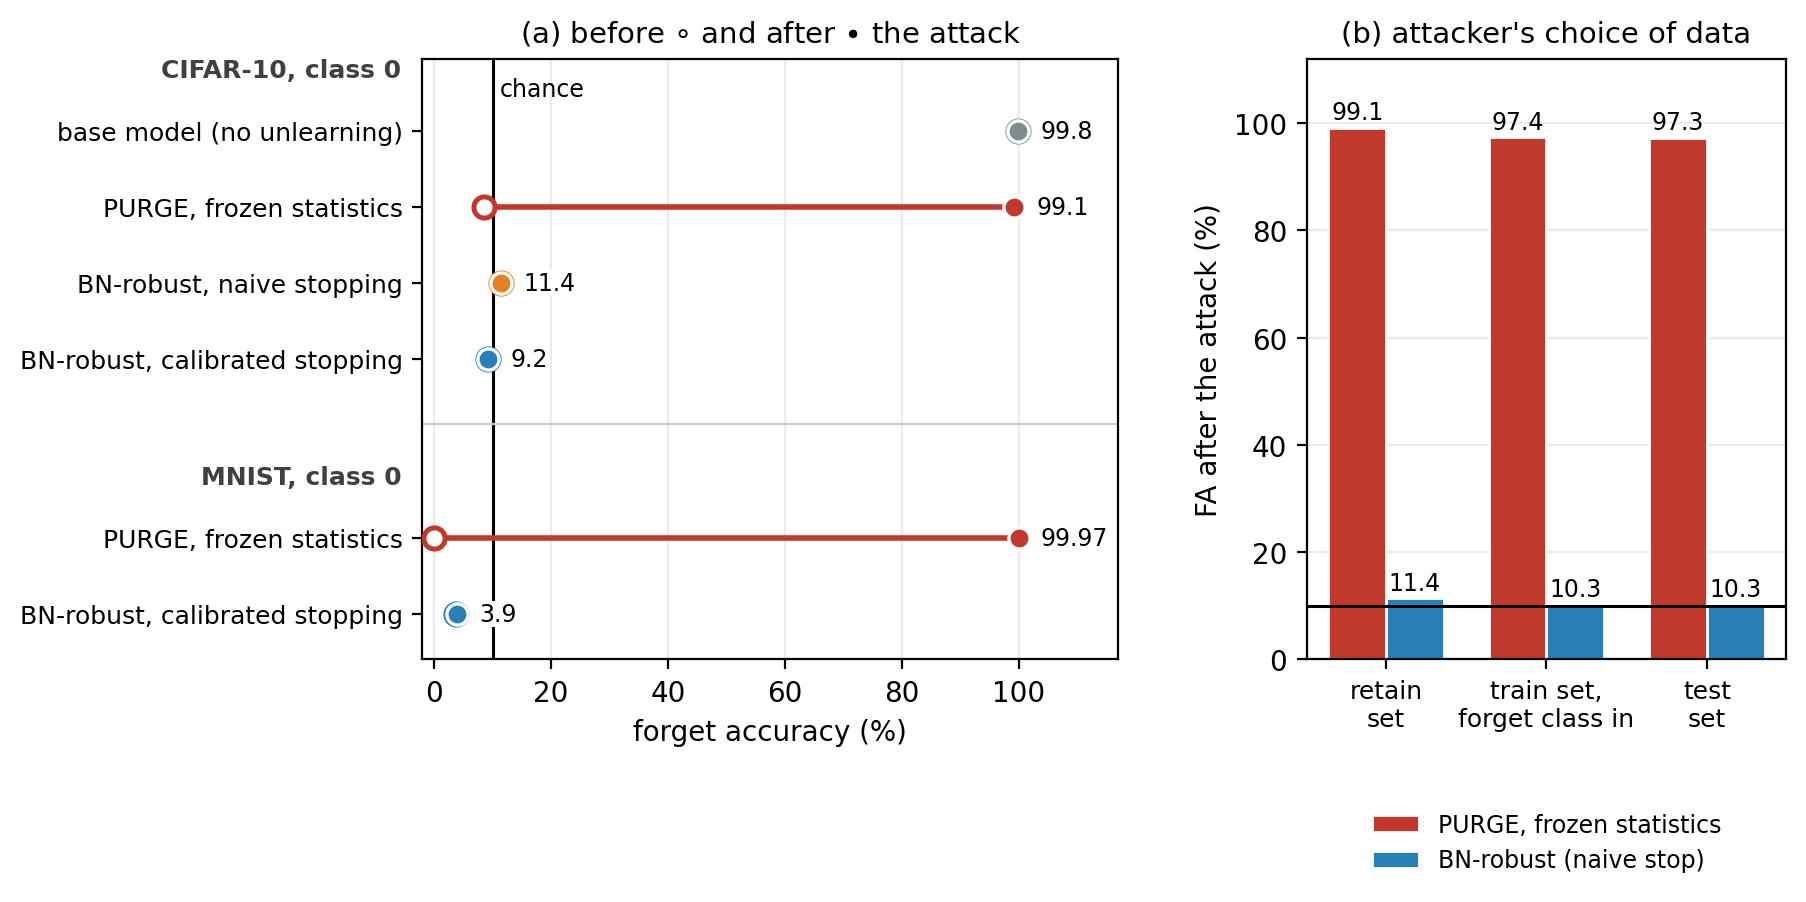
\includegraphics[width=\textwidth]{fig_bnrobust_attack.png}
\caption{\added{\textbf{BN-robust survives the recalibration attack.} (a)~Forget
accuracy before (open) and after (filled) \texttt{update\_bn} on the retain set,
class~0, means over three seeds; on MNIST the frozen configuration's forgetting
is undone completely. (b)~Forget accuracy after the attack when the attacker
recalibrates on the retain set, the full training set (forget class included),
or the test set (CIFAR-10 class~0, three seeds; BN-robust with naive stopping).}}
\label{fig:bnrobust_attack}
\end{figure}

\subsection{Membership Inference Needs a Retrained Reference}\label{sec:mia_main}

\rev{MIA is usually read against $0.5$: an attacker should not be able to tell
forget-class training samples from forget-class test samples. We test that
target against models retrained without the forget class, which trained on
neither group (Table~\ref{tab:mia_main}; Appendix~\ref{sec:mia} adds three
attacks). On CIFAR-10 the reference scores $0.694$ on the loss attack, with a
true-positive rate of $12.5\%$ at $1\%$ false positives, while the base model,
which memorised every member, scores $0.483$: the attack reads a difference in
difficulty between the train and test splits, not membership. Across four
PathMNIST classes the reference ranges from $0.306$ to $0.704$, so no single
constant is the right target. Read against $0.5$, \ours{} looks the worst of the
four methods on CIFAR-10 and SalUn the best; read against the reference, the
order reverses. SalUn's $0.500$ is also degenerate: its true-positive rate is
zero at every threshold, the signature of a constant score. On three of the four
PathMNIST classes \ours{} sits far from its own reference (mean gap
$0.22$--$0.36$ over four attacks), so we claim the protocol finding, not that
\ours{} matches retrained models in general.}

\begin{table}[t]
\centering\color{revisedB}
\caption{\rev{\textbf{Loss-attack MIA against a retrained reference}
(CIFAR-10, class~0). Members are the $5000$ forget-class training images,
non-members the $1000$ forget-class test images; TPR is at $1\%$ FPR.
Appendix~\ref{sec:mia} gives three further attacks and four PathMNIST classes.}}
\label{tab:mia_main}
\small
\begin{tabular}{@{}lccccc@{}}
\toprule
Model & FA & AUROC & TPR & $|\mathrm{AUROC}-0.5|$ & $|\mathrm{AUROC}-\mathrm{ref}|$ \\
\midrule
Retrained (reference) & $0.0$   & $0.694$ & $12.5\%$ & $0.194$ & ---   \\
Base (no unlearning)  & $100.0$ & $0.483$ & $0.0\%$  & $0.017$ & $0.211$ \\
\midrule
SalUn                 & $0.0$   & $0.500$ & $0.0\%$  & $\mathbf{0.000}$ & $0.194$ \\
Bad Teacher           & $24.8$  & $0.485$ & $0.2\%$  & $0.015$ & $0.209$ \\
SCRUB                 & $89.5$  & $0.477$ & $0.4\%$  & $0.023$ & $0.217$ \\
\ours{}               & $2.0$   & $0.693$ & $1.4\%$  & $0.193$ & $\mathbf{0.001}$ \\
\bottomrule
\end{tabular}
\end{table}

\subsection{Further Analyses}\label{sec:further}

The appendices report the remaining experiments in full. \emph{Transformer:} on
ViT-B/16 forgetting transfers \rev{on CIFAR-10}, with FA $9.71\%$ and RA
$97.55\%$, \rev{but not on CIFAR-100 within its 20-epoch cap, where FA ends
between $4.0\%$ and $82.0\%$ across nine classes against a $1\%$ chance level}
(Appendix~\ref{sec:vit}). \emph{Tolerances:} the retain budget is non-binding,
and the forget target is a usable knob over a $29$pp range once it is checked at
every step (Appendix~\ref{sec:sweeps}). \emph{Distance to a retrained model:}
\ours{} is closest in feature space (Fr\'echet distance $13$ against
$153$--$495$ for the baselines) and SalUn in output space
(Appendix~\ref{sec:distance}). \emph{Stopping point:} divergence to a retrained
model is U-shaped along the trajectory with its minimum above chance, and MIA
passes through $0.5$ rather than converging to it
(Appendices~\ref{sec:overforget} and~\ref{sec:trajectory}). \rev{\emph{Sequential
unlearning:} over three classes TA falls from $86.1\%$ to $69.1\%$ and RA from
$100\%$ to $80.7\%$, no more than the forgotten classes themselves account for
(\S\ref{sec:limitations}).}

% ============================================================
\section{Limitations}\label{sec:limitations}

The compute a dataset needs cannot be predicted in advance: the binding resource
is optimiser steps, and STL-10 and CIFAR-100 needed 60 epochs rather than 15 and
20\rev{; ViT-B/16 on CIFAR-100 does not reach chance within its 20-epoch cap}.
Sample-level forgetting works only crudely, because the retain-confusion
target degenerates to uniform when every class remains in the retain set. The
guarantee bounds the sampled mini-batch retain objective, not the population
loss, and holds to float32 precision\rev{; under BN-robust \ours{} it holds per
step under that step's statistics and does not cover the recalibration between
steps}. Our separation from soft conflict-resolution methods
\citep{patel2025learning} is structural; we have not run that method on our
stack. BN-robust \ours{} costs about seven times the compute, was evaluated on
two datasets, and defends only the normalisation statistics, not weight-level
attacks such as fine-tuning recovery\rev{; its comparison with prior methods
rests on the evaluations of \citet{kalani2026batchnorm} and on our own
reproductions, and a like-for-like run of those methods under the same base and
attack remains to be done. In sequential unlearning the retained classes are not
damaged cumulatively, but earlier-forgotten classes partly return: after three
classes RA is $80.7\%$, above the $77.8\%$ that fully forgotten classes would
allow, so they average at least $13\%$ training accuracy, above chance.} \ours{}
gives no differential-privacy guarantee. Appendix~\ref{app:limitations}
discusses each point.

% ============================================================
\section{Conclusion}\label{sec:conclusion}

Unlearning is the dual of continual learning, and \rev{one of continual
learning's most direct tools, a hard constraint on the update, carries over}.
For that constraint to mean anything it must be stated for the update the
optimiser applies: projecting the post-momentum update makes
Theorem~\ref{thm:retain_safety} exact for the deployed optimiser, while the
analysis-friendly alternative \rev{leaves forget accuracy far above chance on
five of six datasets}. Across six datasets and 31 forgetting tasks \ours{}
reaches the chance level on all six (two at a longer budget) with retain
accuracy at or above $97.2\%$ on the 10-class datasets, and \rev{step-level logs
of a CIFAR-10 run} confirm the constraint at every step.
\added{On BatchNorm backbones, keeping the normalisation statistics consistent
with the weights throughout unlearning makes that forgetting survive
recalibration, on every CIFAR-10 class and on MNIST.} The duality is also a
design space: \rev{many continual-learning techniques that protect old-task
knowledge suggest unlearning counterparts} that protect retained knowledge
during erasure. More broadly, when an
optimiser detail is chosen for analytical convenience, it should be checked
against the behaviour it was meant to explain.

\FloatBarrier
% tmlr.bst when available; plainnat keeps the document compilable without it.
\IfFileExists{tmlr.bst}{\bibliographystyle{tmlr}}{\bibliographystyle{plainnat}}
\bibliography{../references}

% ============================================================
\appendix
% ============================================================
\section{Related Work and Positioning in Full}\label{app:related}\label{sec:related_intro}

Approximate unlearning methods occupy different points on the privacy--utility
frontier, and the retain side is where they differ most. \textbf{Gradient
ascent} \citep{thudi2022unrolling} maximises forget-set loss with no mechanism
protecting retain accuracy \rev{(Theorem~\ref{thm:separation}(i))}. \textbf{SalUn} \citep{fan2024salun} confines random-label updates to a
saliency mask---effective in practice, but with no formal retain guarantee and
no control over how much is forgotten. \textbf{SCRUB}
\citep{kurmanji2023unbounded} alternates forget and retain steps balanced by a
weight $\lambda$, so the balance is tuned rather than enforced; in our
reproduction it preserves retain accuracy ($97.7\%$) by barely forgetting at all
(forget accuracy $88.8\%$, Table~\ref{tab:cifar10}). \textbf{NegGrad+}
\citep{thudi2022unrolling} adds a retain-loss term as a weighted sum, again
without a guarantee that retain loss is controlled. Closest to us,
\citet{patel2025learning} diagnose the same forget--retain gradient conflict but
resolve it with a soft regulariser that rewards positive alignment. A fuller treatment, including exact unlearning and distillation-based methods, follows the table.

The distinction we draw is structural rather than numerical, so
Table~\ref{tab:properties} compares properties of each method's \emph{definition}
---checkable against the published update rule, without relying on our
reimplementation of it. A soft penalty biases the optimiser toward retain-safe
steps but leaves harmful steps feasible: for any finite penalty weight, a
sufficiently large forget-loss reduction still makes a retain-harming step
preferable. A projection removes those steps from the feasible set altogether
(Theorem~\ref{thm:separation}(iv)). The final row is the one we would emphasise,
and the one \S\ref{sec:momentum_ablation} makes concrete: a guarantee proved for
a momentum-free surrogate says nothing about a run that uses momentum.

\rev{Figure~\ref{fig:teaser}} places the method against the alternatives on both
what it achieves and what it guarantees.

\paragraph{Exact unlearning.}
SISA \citep{bourtoule2021sisa} partitions data into shards so that removal
requires retraining only the affected shard; the per-deletion cost approaches
full retraining as shard count grows. Certified removal
\citep{guo2020certified} gives exact guarantees for convex models but does not
extend to deep networks.

\paragraph{Gradient-based approximate unlearning.}
GA \citep{thudi2022unrolling} maximises forget-set loss, with no mechanism to
prevent the same direction from degrading retain performance. Amnesiac
unlearning \citep{graves2021amnesiac} subtracts cached per-sample updates,
requiring $O(T|\Df|)$ storage. NegGrad+ optimises
$-\lossf + \lambda\lossr$ directly, which is the Lagrangian relaxation of
Eq.~\ref{eq:problem} rather than a solution to it: the retain term shifts the
optimum without bounding any single step, so the weighted sum is exactly the
soft treatment Theorem~\ref{thm:separation}(iv) separates us from.

\paragraph{Saliency and Fisher methods.}
SalUn \citep{fan2024salun} applies random-label updates inside a top-50\%
saliency mask: strong empirically (FA~$=0\%$ on CIFAR-10) but with no formal
retain guarantee and no control over the degree of forgetting. Fisher-based
methods \citep{golatkar2020eternal,golatkar2021scrubbing} and SSD
\citep{foster2024ssd} weight parameters by estimated importance, requiring
Hessian approximations that scale poorly.

\paragraph{Knowledge distillation.}
Bad Teacher \citep{chundawat2023badteacher} uses competent/incompetent teachers.
SCRUB \citep{kurmanji2023unbounded} is closest in motivation---both draw on CL
intuitions and use KD to anchor retain behaviour---but differs algorithmically:
SCRUB alternates forget and retain steps balanced by $\lambda$, so its balance is
hyperparameter-dependent, whereas \ours{}'s retain safety holds by construction
(Theorem~\ref{thm:separation}); and SCRUB ascends the forget loss, which is
unstable in either direction, whereas \klr{} converges to a specific target
distribution.

\paragraph{Continual learning connection, and the closest prior work.}
A-GEM \citep{chaudhry2019agem} projects task gradients to avoid catastrophic
forgetting. The CL--MU duality has been noted conceptually
\citep{nguyen2020variational,kurmanji2023unbounded}. Closest to \ours{}, recent
work \citep{patel2025learning} also targets the forget--retain gradient
conflict, but through an \emph{implicit, soft} regulariser encouraging a positive
inner product---with no per-step constraint and no formal guarantee. More
broadly, gradient projection and conflict resolution are now actively explored
for unlearning. \added{Closest in mechanism is Projected-Gradient Unlearning
\citep{hoang2024learn}, which takes unlearning steps orthogonal to a gradient
subspace estimated for the retained data. \ours{} differs in the constraint and in
what it binds: a half-space against the current retain gradient---the minimum
correction that excludes retain-harming steps---applied to the post-momentum
update the optimiser actually takes.} \ours{} enforces $\langle u_t,\gr\rangle \ge 0$ explicitly at every
step, on the post-momentum update, which is the difference between \emph{softly
discouraging} conflict and \emph{provably eliminating} it---and, relative to
guarantees stated for momentum-free surrogates, the difference between a bound
that describes the deployed optimiser and one that does not.
\S\ref{sec:strength} tests the mechanism this distinction rests on by varying
our own projection between a soft penalty and the hard constraint; a
like-for-like run of that method on our stack remains future work.

% ============================================================
\section{Design Details}\label{app:method}

\subsection{From the Optimisation Problem to the Algorithm}

This framing makes three things explicit that weighted multi-objective
approaches conflate. First, retain safety is a \emph{hard constraint}, not a
soft penalty. Second, \rev{the forget objective sets the direction of the
search and the forget-accuracy target its end point; only the second is a
constraint}. Third, the two tolerances \rev{$(\alpha, \tau_F)$} are quantities a
practitioner sets, not epochs to be tuned.

\paragraph{Why this needs a new algorithm.} Writing down
Eq.~\ref{eq:problem} is not by itself progress: one could hand it to a generic
constrained solver, or relax it into the weighted objective that existing
methods already optimise. Both routes lose the property we are after. A
Lagrangian relaxation replaces the retain constraint with a penalty
$\lambda\,\lossr$, which is precisely the soft treatment whose feasible set still
contains retain-harming steps (Theorem~\ref{thm:separation}(iv)); and a
projected-gradient solver applied naively would enforce feasibility on the
gradient while the optimiser applies something else
(Proposition~\ref{prop:counter}). What the problem \emph{does} buy is a
specification: it says exactly which quantity each mechanism must control.
\rev{\ours{} realises each condition with the cheapest mechanism we know that
enforces it, and enforces retain safety at every step on the vector actually
applied.} Table~\ref{tab:constraint_map} states that correspondence, and
\S\ref{sec:method} derives each row.

\begin{table}[t]
\centering
\caption{\rev{\textbf{From the problem to the algorithm.} Each condition of
Eq.~\ref{eq:problem}, and the property of the search path, with the mechanism
that enforces it. Two components serve no condition directly: the distillation
anchor, which is part of the retain objective the projection protects, and the
handling of BatchNorm statistics (\S\ref{sec:bn}).}}
\label{tab:constraint_map}
\color{revisedB}
\begin{tabular}{@{}p{0.31\textwidth}p{0.33\textwidth}p{0.28\textwidth}@{}}
\toprule
\textbf{Condition} & \textbf{Mechanism} & \textbf{Enforced} \\
\midrule
Retain objective does not increase along the path &
Projection of the post-momentum update onto $\{\langle u,\gr\rangle \ge 0\}$ (\S\ref{sec:projection}--\ref{sec:optimiser}) &
Every step, to first order on the sampled batch (Thm.~\ref{thm:retain_safety}) \\
\addlinespace
$\CE(\theta;\Dr) \le \alpha\,\CE(\theta_0;\Dr)$ &
Retain-loss stopping rule (\S\ref{sec:stopping}) &
After every epoch, on the full retain set \\
\addlinespace
$\mathrm{FA}(\theta;\Df) \le \tau_F$ &
Forget-accuracy stopping rule (\S\ref{sec:stopping}) &
Every $m$ steps \\
\addlinespace
Direction of the search &
\klr{}: descend $\KL(p_\theta(x_f)\|p_r)$ (\S\ref{sec:forget_obj}) &
Every step \\
\addlinespace
$\|\theta - \theta_0\| \le R$ &
Clipping before accumulation, and the step budget &
$\|\theta_N - \theta_0\| \le N\eta c/(1-\mu)$ \\
\bottomrule
\end{tabular}
\end{table}

\subsection{What Is Taken from A-GEM, and What Is Not}

The operator in
Eq.~\ref{eq:projection} is A-GEM's, and we claim no novelty for it: the
correction $v \mapsto v - \frac{\langle v,g\rangle}{\|g\|^2}g$ is the standard
projection onto a half-space, and \citet{chaudhry2019agem} introduced its use in
continual learning with $g$ the gradient on an episodic memory of past tasks. We
also inherit its two attractive properties: it is the \emph{minimum-norm}
correction restoring feasibility, so it is the least destructive repair of a
conflicting step, and it costs one extra backward pass and one inner product per
step.

What is new is what the operator is asked to do. In A-GEM the projection is a
safeguard on a process whose objective already points the right way---the new
task is being learned, and the memory gradient only occasionally interferes; in
our runs the conflict is not occasional but universal, firing at $100\%$ of
steps (\S\ref{sec:alignment}), because erasing a class and preserving the rest
are directly opposed rather than incidentally so. The projection is therefore
not a correction applied to an optimiser but the optimiser's defining step. That
change of role has three consequences, and they are what
\S\ref{sec:optimiser} is about:
\begin{enumerate}
\item \emph{It must bind the applied vector.} A-GEM projects a gradient; with
momentum the applied vector is not the gradient, and projecting the gradient
certifies nothing (Proposition~\ref{prop:counter}).
\item \emph{Its magnitude matters.} A-GEM tolerates $\|\Pi_{\gr}(v)\| \le \|v\|$
because progress on the new task comes mostly from unconflicted steps. When
every step conflicts, that contraction compounds and forgetting stalls, so we
restore the norm after projecting.
\item \emph{It bounds nothing on the forget side.} The projection guarantees
retain safety and only that; on its own it does not unlearn. Our projection-only
ablation reaches forget accuracy $18.66\%$ against a $10\%$ chance level
(Table~\ref{tab:cifar10}), which is why \ours{} pairs it with a forget objective
rather than presenting the projection as a method.
\end{enumerate}

\subsection{The Three Ordering Choices}

\ours{} uses SGD with momentum $\mu$, weight decay $\lambda_{\mathrm{wd}}$, and
gradient clipping $c$. Three ordering choices determine whether the guarantee is
real, and all three matter empirically.

\paragraph{(i) Project the update, not the gradient.}
The vector applied to the weights is $u_t$, not $\gf$. We therefore
momentum-accumulate first and project afterwards
(Algorithm~\ref{alg:excise}, lines 10--15), so that
$\langle u_t,\gr\rangle \ge 0$ holds for the update that is actually applied.
Projecting $\gf$ instead leaves $\langle u_t,\gr\rangle$ unconstrained.

\paragraph{(ii) Clip before accumulating.}
Clipping is applied to the per-step ingredient $d_t$ \emph{before} it enters the
momentum buffer. This preserves the standard SGD semantics in which momentum
accumulates clipped gradients, and yields the bound
$\|v_t\| \le c/(1-\mu)$ used in Theorem~\ref{thm:retain_safety}. Clipping the
final update instead would cap $\|u_t\| \le c$, destroying the
$1/(1-\mu)$ amplification that momentum provides; since raw forget gradients are
${\sim}100\times$ the clip threshold in our runs, clipping is always active, and
this ordering is the difference between forgetting and not forgetting.

\paragraph{(iii) Preserve magnitude under projection.}
Projection is norm-non-increasing: $\|\Pi_{\gr}(v)\| = \|v\|\sin\vartheta$ where
$\vartheta$ is the angle between $v$ and $\gr$. When forget and retain gradients
are nearly antiparallel, $\sin\vartheta \approx 0$ and the applied step
collapses, stalling forgetting for reasons unrelated to retain safety. We
therefore rescale the projected update to the pre-projection norm,
$u_t = \Pi_{\gr}(v_t)\,\|v_t\|/\|\Pi_{\gr}(v_t)\|$. Because
$\langle u,\gr\rangle = 0$ is invariant to positive rescaling, this leaves the
guarantee untouched while decoupling forgetting speed from conflict severity.
(If $\Pi_{\gr}(v_t)=0$, i.e.\ $v_t$ is exactly antiparallel to $\gr$, we set
$u_t=0$; the guarantee holds trivially.)

\subsection{The Forget Objective}

The \klr{} objective of Eq.~\ref{eq:kl_retain} targets $p_r$,
where $p_r$ (Eq.~\ref{eq:retain_confuse}) is the model's natural confusion
pattern. The motivation is that no trained model produces uniform outputs, so a
model driven toward $\mathcal{U}(K)$ remains separable from a retrained one even
at FA~$=0\%$; a forget target drawn from the model's own behaviour on retained
data does not have that artefact. Under the previous implementation this was
supported empirically, with the uniform target giving MIA AUROC~$=0.469$ against
$0.496$ for \klr{}. \textbf{Re-measured under the projected-momentum optimiser,
it is not.} The three forget objectives give, on CIFAR-10 class~0:
gradient ascent $\mathrm{TA}/\mathrm{FA}/\mathrm{MIA} = 86.4/8.2/0.559$,
KL-uniform $86.4/3.9/0.526$, and \klr{} $86.1/2.1/0.528$. Both KL variants
clearly beat gradient ascent, which neither forgets as far nor stays as close to
the ideal MIA. Between the two, however, the difference is within noise and if
anything favours uniform ($|\mathrm{MIA}-0.5| = 0.026$ against $0.028$).

We therefore keep \klr{} for its lower forget accuracy at equal test accuracy,
and retract the claim that it is distinguishable from the uniform target on
MIA grounds. This is consistent with \S\ref{sec:overforget}: $p_r$ is not what a
retrained model produces on forget inputs, so an argument resting on $p_r$ being
the ``natural'' target was never on firm ground. What survives is narrower---%
$p_r$ is a better forget \emph{direction} than uniform, and no more. It is not a claim that $p_r$ is what a retrained model
outputs on forget inputs: \S\ref{sec:overforget} and
Appendix~\ref{app:d2r} show it is not, and that minimising the divergence to it
is harmful.

\subsection{Supporting Components}

\paragraph{KD-anchored stability.}
A frozen copy of $\theta_0$ serves as teacher,
$\losskd = T^2\KL(\sigma(f_\theta(x_r)/T)\|\sigma(f_{\theta_0}(x_r)/T))$,
anchoring behaviour on $\Dr$ and complementing the projection.

\section{Notation, Assumptions, and the Analysed Update}\label{app:setup}

We restate the update exactly as implemented, since the entire point of
Theorem~\ref{thm:retain_safety} is that the analysed object and the executed
object coincide.

\paragraph{Notation.}
\rev{$\Lrt(\theta)$ is the retain objective $\lossr$ of
\S\ref{sec:problem}---cross-entropy plus $\beta\losskd(\theta,\theta_0;\Dr)$---}%
evaluated on the sampled retain mini-batch at step $t$, and $\gr := \nabla_\theta\Lrt(\theta_t)$ its gradient. Note $\beta$ does not
appear separately in the bounds because $\gr$ is already the composite gradient.
$\gf := \nabla_\theta\lossf(\theta_t;x_f)$ is the forget gradient on the forget
mini-batch. $\lambda_{\mathrm{wd}} \ge 0$ is weight decay, $c>0$ the clipping
threshold, $\eta>0$ the learning rate, and $\mu\in[0,1)$ the momentum
coefficient. $\|\cdot\|$ is the Euclidean norm on the concatenation of all
trainable parameters.

\paragraph{The projection operator.}
For $g \ne 0$ define
\begin{equation}\label{eq:app_proj}
\Pi_{g}(v) \;=\;
\begin{cases}
v, & \langle v,g\rangle \ge 0,\\[2pt]
v - \dfrac{\langle v,g\rangle}{\|g\|^{2}}\,g, & \langle v,g\rangle < 0,
\end{cases}
\qquad
\widehat{\Pi}_{g}(v) \;=\;
\begin{cases}
\Pi_g(v)\,\dfrac{\|v\|}{\|\Pi_g(v)\|}, & \Pi_g(v) \ne 0,\\[4pt]
0, & \Pi_g(v) = 0,
\end{cases}
\end{equation}
where $\widehat{\Pi}$ is the \emph{magnitude-preserving} variant used by \ours{}
(\S\ref{sec:optimiser}). In the implementation the case $\Pi_g(v)=0$ is detected
by the guard $\|\Pi_g(v)\| \le \epsilon\|v\|$ with $\epsilon = 10^{-8}$.

\paragraph{The analysed (and executed) update.}
With $v_{-1}=0$, for $t = 0,1,2,\dots$
\begin{align}
d_t &= \mathrm{clip}_c\!\big(\gf^{(t)} + \lambda_{\mathrm{wd}}\theta_t\big),
      &&\text{where } \mathrm{clip}_c(x) = x\cdot\min\!\big(1, c/\|x\|\big),
      \label{eq:app_clip}\\
v_t &= \mu\,v_{t-1} + d_t, \label{eq:app_mom}\\
u_t &= \widehat{\Pi}_{\gr^{(t)}}(v_t), \label{eq:app_projstep}\\
\theta_{t+1} &= \theta_t - \eta\,u_t. \label{eq:app_step}
\end{align}
Three orderings are load-bearing and are stated here so they cannot be lost in
implementation: clipping acts on $d_t$ \emph{before} the momentum accumulation
(\ref{eq:app_clip})--(\ref{eq:app_mom}); the projection acts on the accumulated
$v_t$, i.e.\ on the update rather than on the gradient (\ref{eq:app_projstep});
and no clipping is applied after (\ref{eq:app_projstep}).

\paragraph{Assumptions.}
\begin{itemize}
\item[(A1)] $\Lrt$ is $L$-smooth: $\|\nabla\Lrt(x)-\nabla\Lrt(y)\| \le L\|x-y\|$
for all $x,y$.
\item[(A2)] Clipping is applied as in (\ref{eq:app_clip}), so $\|d_t\| \le c$ for
all $t$.
\item[(A3)] $\mu \in [0,1)$.
\end{itemize}
(A1) is the standard smoothness assumption of first-order analysis; for ReLU
networks it holds piecewise, and we treat it as an idealisation, as is
conventional. (A2) and (A3) are properties of the implementation, not
assumptions about the data.

% ------------------------------------------------------------
\section{Proof of Theorem~\ref{thm:retain_safety}}\label{app:thm1}

We prove three lemmas and then assemble the theorem.

\begin{lemma}[Projection properties]\label{lem:proj}
Let $g \ne 0$ and $v$ be arbitrary. Then
\begin{enumerate}
\item[(i)] $\langle \Pi_g(v), g\rangle \ge 0$, with equality whenever
$\langle v,g\rangle < 0$;
\item[(ii)] $\|\Pi_g(v)\| \le \|v\|$;
\item[(iii)] $\langle \widehat{\Pi}_g(v), g\rangle \ge 0$ and
$\|\widehat{\Pi}_g(v)\| \le \|v\|$, with $\|\widehat{\Pi}_g(v)\| = \|v\|$
whenever $\Pi_g(v)\ne 0$.
\end{enumerate}
\end{lemma}

\begin{proof}
(i) If $\langle v,g\rangle \ge 0$ then $\Pi_g(v)=v$ and the claim is immediate.
If $\langle v,g\rangle<0$ then
\[
\langle \Pi_g(v), g\rangle
= \Big\langle v - \tfrac{\langle v,g\rangle}{\|g\|^2}g,\; g\Big\rangle
= \langle v,g\rangle - \tfrac{\langle v,g\rangle}{\|g\|^2}\|g\|^2 = 0 .
\]
(ii) In the first branch this is an equality. In the second branch, $\Pi_g$ is
the orthogonal projection onto the hyperplane $\{u:\langle u,g\rangle=0\}$;
writing $v = \Pi_g(v) + \tfrac{\langle v,g\rangle}{\|g\|^2}g$ as a sum of two
orthogonal vectors, Pythagoras gives
\begin{equation}\label{eq:app_pyth}
\|v\|^2 = \|\Pi_g(v)\|^2 + \frac{\langle v,g\rangle^2}{\|g\|^2}
\;\ge\; \|\Pi_g(v)\|^2 .
\end{equation}
(iii) If $\Pi_g(v)=0$ then $\widehat{\Pi}_g(v)=0$ and both claims are trivial.
Otherwise $\widehat{\Pi}_g(v) = s\,\Pi_g(v)$ with
$s = \|v\|/\|\Pi_g(v)\| > 0$, so
$\langle \widehat{\Pi}_g(v),g\rangle = s\langle \Pi_g(v),g\rangle \ge 0$ by (i),
and $\|\widehat{\Pi}_g(v)\| = s\|\Pi_g(v)\| = \|v\|$.
\end{proof}

Part (iii) is the formal content of the design choice in
\S\ref{sec:optimiser}(iii): rescaling restores the magnitude that
(\ref{eq:app_pyth}) removes, and because $s>0$ it cannot flip the sign of the
inner product. The guarantee is therefore invariant to the rescaling, while the
step magnitude is not.

\begin{lemma}[Velocity norm bound]\label{lem:vel}
Under (A2) and (A3), for every $t \ge 0$,
\begin{equation}\label{eq:app_velbound}
\|v_t\| \;\le\; c\,\frac{1-\mu^{\,t+1}}{1-\mu} \;<\; \frac{c}{1-\mu}.
\end{equation}
\end{lemma}

\begin{proof}
Unrolling (\ref{eq:app_mom}) from $v_{-1}=0$ gives
$v_t = \sum_{k=0}^{t}\mu^{\,t-k} d_k$. By the triangle inequality and (A2),
\[
\|v_t\| \;\le\; \sum_{k=0}^{t}\mu^{\,t-k}\|d_k\|
\;\le\; c\sum_{j=0}^{t}\mu^{\,j}
\;=\; c\,\frac{1-\mu^{\,t+1}}{1-\mu}
\;<\; \frac{c}{1-\mu},
\]
the last step using $\mu\in[0,1)$ so that $\mu^{t+1}>0$ and the geometric series
converges.
\end{proof}

Lemma~\ref{lem:vel} is where the clip-before-momentum ordering is used: it
requires $\|d_k\|\le c$ for the \emph{ingredients} of the sum. Note also that the
bound is attained only in the limit of perfectly aligned successive steps; we
observe $\max_t\|u_t\| = 9.16$ against $c/(1-\mu)=10$ in
\S\ref{sec:alignment}, so it is tight in practice.

\begin{lemma}[Descent step]\label{lem:descent}
Under (A1), for any vector $u$ and $\theta_{+} = \theta_t - \eta u$,
\begin{equation}\label{eq:app_descent}
\Lrt(\theta_{+}) \;\le\; \Lrt(\theta_t) - \eta\langle u, \gr\rangle
+ \tfrac{1}{2}L\eta^2\|u\|^2 .
\end{equation}
\end{lemma}

\begin{proof}
Standard consequence of $L$-smoothness (the descent lemma): (A1) implies
$\Lrt(y) \le \Lrt(x) + \langle \nabla\Lrt(x), y-x\rangle + \tfrac{L}{2}\|y-x\|^2$
for all $x,y$. Substituting $x=\theta_t$, $y=\theta_+$, so that
$y-x = -\eta u$ and $\nabla\Lrt(x)=\gr$, gives (\ref{eq:app_descent}).
\end{proof}

\begin{theorem}[Theorem~\ref{thm:retain_safety}, restated]\label{thm:app_main}
Under (A1)--(A3), the update (\ref{eq:app_clip})--(\ref{eq:app_step}) satisfies,
at every step $t$ and unconditionally,
\begin{align}
\text{(a)}\quad & \langle u_t, \gr^{(t)}\rangle \;\ge\; 0, \label{eq:app_a}\\
\text{(b)}\quad & \|u_t\| \;\le\; \|v_t\| \;<\; \frac{c}{1-\mu},
   \quad\text{with }\|u_t\|=\|v_t\|\text{ unless }\Pi_{\gr}(v_t)=0,
   \label{eq:app_b}\\
\text{(c)}\quad & \Lrt(\theta_{t+1}) \;\le\; \Lrt(\theta_t)
   + \tfrac{1}{2}L\eta^{2}\Big(\frac{c}{1-\mu}\Big)^{\!2}. \label{eq:app_c}
\end{align}
\end{theorem}

\begin{proof}
(a) Immediate from Lemma~\ref{lem:proj}(iii) applied to $v_t$ with
$g=\gr^{(t)}$, using (\ref{eq:app_projstep}). If $\gr^{(t)}=0$ the projection is
undefined and is skipped; then $\langle u_t,\gr^{(t)}\rangle = 0$ and (a) holds
trivially (see Remark~\ref{rem:degenerate}).

(b) Combine Lemma~\ref{lem:proj}(iii) with Lemma~\ref{lem:vel}.

(c) By Lemma~\ref{lem:descent} with $u = u_t$,
\[
\Lrt(\theta_{t+1}) \le \Lrt(\theta_t) - \eta\underbrace{\langle u_t,\gr^{(t)}\rangle}_{\ge\,0\ \text{by (a)}}
+ \tfrac{1}{2}L\eta^2\underbrace{\|u_t\|^2}_{<\,(c/(1-\mu))^2\ \text{by (b)}}
\;\le\; \Lrt(\theta_t) + \tfrac{1}{2}L\eta^2\Big(\frac{c}{1-\mu}\Big)^{\!2}. \qedhere
\]
\end{proof}

The first-order change in the sampled retain objective is thus non-positive at
every step; the only admissible increase is the $O(\eta^2)$ curvature term. The
guarantee is \emph{unconditional} in the sense that it requires no assumption on
$\gf$, on the alignment between forget and retain gradients, or on the data.

\begin{corollary}[Momentum-free reduction]\label{cor:mu0}
Setting $\mu=0$ gives $v_t = d_t$, $\|u_t\|\le c$, and
$\Lrt(\theta_{t+1}) \le \Lrt(\theta_t) + \tfrac{1}{2}L\eta^2c^2$, recovering the
momentum-free per-step bound.
\end{corollary}

\begin{corollary}[A-GEM reduction]\label{cor:agem}
Setting $\mu=0$, $c=\infty$ and letting $\eta\to0$ recovers the first-order
A-GEM guarantee $\langle u_t,\gr\rangle\ge0$ \citep{chaudhry2019agem}.
\end{corollary}

Corollary~\ref{cor:mu0} is worth reading alongside
Table~\ref{tab:momentum}: the $\mu=0$ bound is \emph{formally tighter} (by a
factor $(1-\mu)^{-2}=100$ at $\mu=0.9$), yet the configuration it describes
fails to unlearn on five of six datasets. A tighter bound on a method that does
not forget is not the better result---which is precisely why we analyse the
update that is actually run.

\subsection{Why the Projection Must Be Applied to the Update}\label{app:counterexample}

The following proposition shows that the design choice of
\S\ref{sec:optimiser}(i) is not a matter of convenience: projecting the
\emph{gradient} provides no per-step guarantee once $\mu>0$, however carefully
each individual gradient is projected.

\begin{proposition}[Gradient-projection is insufficient under momentum]\label{prop:counter}
Consider the variant that projects the gradient and then accumulates momentum:
\[
\tilde d_t = \mathrm{clip}_c\big(\Pi_{\gr^{(t)}}(\gf^{(t)})\big), \qquad
v_t = \mu v_{t-1} + \tilde d_t, \qquad \theta_{t+1} = \theta_t - \eta v_t ,
\]
so that every accumulated ingredient satisfies
$\langle \tilde d_t, \gr^{(t)}\rangle \ge 0$. Then for every $\mu \in (0,1)$
there exist retain and forget gradients for which the applied update $v_t$
satisfies $\langle v_t, \gr^{(t)}\rangle < 0$, i.e.\ the step strictly increases
the sampled retain loss to first order.
\end{proposition}

\begin{proof}
Work in $\mathbb{R}^2$ with $\lambda_{\mathrm{wd}}=0$, $c=\infty$ (clipping
inactive), and $v_{-1}=0$.

\emph{Step $0$.} Let $\gr^{(0)} = (1,0)$ and $\gf^{(0)} = (-1,1)$. Then
$\langle \gf^{(0)},\gr^{(0)}\rangle = -1 < 0$, so the projection fires:
\[
\tilde d_0 = \Pi_{\gr^{(0)}}(\gf^{(0)})
= (-1,1) - \frac{-1}{1}(1,0) = (0,1),
\]
which is retain-safe, $\langle \tilde d_0, \gr^{(0)}\rangle = 0$. Hence
$v_0 = (0,1)$.

\emph{Step $1$.} Let the retain mini-batch change so that
$\gr^{(1)} = (0,-1)$, and let $\gf^{(1)} = (1,0)$. Then
$\langle \gf^{(1)},\gr^{(1)}\rangle = 0 \ge 0$, so no projection is needed and
$\tilde d_1 = (1,0)$, again retain-safe:
$\langle \tilde d_1,\gr^{(1)}\rangle = 0$. The applied update is
\[
v_1 = \mu v_0 + \tilde d_1 = \mu(0,1) + (1,0) = (1,\mu),
\qquad
\langle v_1, \gr^{(1)}\rangle = \langle (1,\mu), (0,-1)\rangle = -\mu \;<\; 0
\]
for every $\mu>0$. By Lemma~\ref{lem:descent} the first-order change in $\Lrt$
is $-\eta\langle v_1,\gr^{(1)}\rangle = +\eta\mu > 0$: the retain loss strictly
increases to first order, even though \emph{every} projected gradient entering
the buffer was individually retain-safe.
\end{proof}

The mechanism is transparent: the momentum buffer carries a direction that was
certified against $\gr^{(0)}$ into a step whose constraint is $\gr^{(1)}$, and
the projection at step $1$ never inspects the carried term. Projecting $v_t$
itself (\ref{eq:app_projstep}) removes exactly this failure, because the
certificate is issued against the constraint in force at the step where the
update is applied. Note also that $\mu$ appears linearly in the violation, so the
defect grows with the momentum coefficient rather than vanishing.

\subsection{Why Clipping Must Precede Accumulation}\label{app:clip_order}

\begin{proposition}[Clipping the update destroys momentum amplification]\label{prop:clip}
Consider the variant that clips the final update,
$u_t = \mathrm{clip}_c(\widehat{\Pi}_{\gr}(\mu v_{t-1} + \tilde g_t))$ with
$\tilde g_t$ unclipped. Then $\|u_t\| \le c$ for all $t$, identical to the bound
obtained at $\mu=0$ (Corollary~\ref{cor:mu0}), irrespective of $\mu$.
\end{proposition}

\begin{proof}
Immediate from the definition of $\mathrm{clip}_c$.
\end{proof}

Proposition~\ref{prop:clip} is trivial as mathematics but decisive in practice.
In our runs the raw forget-gradient norm is ${\sim}100\times$ the clipping
threshold ($\|\gf\| \in [102,149]$ with $c=1$ on CIFAR-10), so clipping is active
at every step and the cap is always attained. Clipping after accumulation
therefore yields an applied step of magnitude exactly $\eta c$ --- the same
magnitude as the momentum-free configuration, and hence the same failure to
forget documented in Table~\ref{tab:momentum}. The ordering in
(\ref{eq:app_clip})--(\ref{eq:app_mom}) instead admits
$\|v_t\| \to c/(1-\mu)$, a $10\times$ larger step at $\mu=0.9$, while
Lemma~\ref{lem:vel} keeps it bounded. The bound in (\ref{eq:app_c}) is looser by
$(1-\mu)^{-2}$ as a result; this is the price of a guarantee that describes an
optimiser that unlearns.

\subsection{Remarks on Scope and Exactness}

\begin{remark}[Mini-batch scope]\label{rem:minibatch}
$\gr^{(t)}$ is the gradient of the retain objective on the \emph{sampled} retain
mini-batch, so (\ref{eq:app_c}) is exact for that mini-batch's objective---which
is the quantity \ours{} projects against, and therefore the quantity about which
a per-step statement can be made. Because mini-batch gradients are unbiased
estimates of the population gradient, the first-order term is non-positive in
expectation up to the standard SGD gradient-variance term; a population-exact
per-step guarantee would require the full retain gradient at every step, at
$O(|\Dr|)$ cost per update. We regard this as the principal formal limitation
(\S\ref{sec:limitations}).
\end{remark}

\begin{remark}[Degenerate retain gradient]\label{rem:degenerate}
The implementation skips the projection when $\|\gr\|^2 < 10^{-12}$, since
(\ref{eq:app_proj}) is then numerically ill-posed. In that regime the violation
of (\ref{eq:app_a}) is bounded by Cauchy--Schwarz:
$|\langle u_t,\gr\rangle| \le \|u_t\|\|\gr\| \le 10^{-6}c/(1-\mu)$, giving a
first-order retain increase of at most $10^{-5}\eta$. Moreover such a $\gr$
means the retain mini-batch is already at a stationary point. The exception is
therefore quantitatively negligible, but we state it rather than suppress it.
\end{remark}

\begin{remark}[Floating-point exactness]\label{rem:float}
In exact arithmetic $\langle \Pi_g(v),g\rangle = 0$ identically. In float32, the
inner products are sums over $1.12\times10^7$ parameters, with accumulation
error of order $\sqrt{n}\,\varepsilon_{32} \approx 4\times10^{-4}$ relative.
The measured worst-case relative violation is $-7.4\times10^{-7}$
(\S\ref{sec:alignment}), three orders of magnitude \emph{below} that scale and
with positive mean, consistent with rounding rather than a systematic defect. We
therefore state Theorem~\ref{thm:app_main} as holding to float32 precision, and
recommend float64 accumulation for the inner products in
(\ref{eq:app_proj}) in reference implementations.
\end{remark}

% ------------------------------------------------------------
\section{Proof of Theorem~\ref{thm:separation}}\label{app:thm2}

\begin{theorem}[Theorem~\ref{thm:separation}, restated]\label{thm:app_sep}
Fix $\theta_0$ with retain gradient $\gr := \nabla\Lrt(\theta_0) \ne 0$ and
forget gradient $\gf$. Consider one-step update operators. Then:
\begin{enumerate}
\item[(i)] \textbf{GA.} The update $\theta_0 + \eta\gf$ strictly increases
$\Lrt$ to first order whenever $\langle \gf,\gr\rangle > 0$.
\item[(ii)] \textbf{SCRUB.} For any fixed $\lambda>0$ there exist $\gf,\gr$ with
$\langle -\gf+\lambda\gr,\;\gr\rangle < 0$.
\item[(iii)] \textbf{SalUn.} The masked random-label update
$-M\odot\nabla\CE_{\mathrm{RL}}$ has unconstrained sign with respect to $\gr$.
\item[(iv)] \textbf{Soft conflict regularisers.} Penalising negative alignment
does not preclude it.
\item[(v)] \textbf{\ours{}.} $\langle u_t,\gr\rangle \ge 0$ unconditionally.
\end{enumerate}
\end{theorem}

\begin{proof}
(i) A first-order expansion gives
$\Lrt(\theta_0+\eta\gf) = \Lrt(\theta_0) + \eta\langle \gf,\gr\rangle + O(\eta^2)$,
which exceeds $\Lrt(\theta_0)$ for small $\eta>0$ when
$\langle\gf,\gr\rangle>0$. Since GA constrains neither the sign nor the
magnitude of $\langle\gf,\gr\rangle$, no configuration-independent per-step
guarantee is available.

(ii) Compute
$\langle -\gf+\lambda\gr,\;\gr\rangle = -\langle\gf,\gr\rangle+\lambda\|\gr\|^2$.
This is negative precisely when
$\langle\gf,\gr\rangle > \lambda\|\gr\|^2$. Such a pair exists for any fixed
$\lambda$: e.g.\ in $\mathbb{R}^2$ take $\gr=(1,0)$ and
$\gf = (\lambda+1)\,(1,0)$, giving
$\langle\gf,\gr\rangle = \lambda+1 > \lambda = \lambda\|\gr\|^2$. Because
$\lambda$ is a fixed hyperparameter while $\langle\gf,\gr\rangle/\|\gr\|^2$
varies along the trajectory, no fixed $\lambda$ certifies every step.

(iii) With random labels the masked gradient direction is uncorrelated with
$\gr$ in expectation; individual draws therefore realise either sign of
$\langle g_{\mathrm{SalUn}},\gr\rangle$, and the mask $M$ (selected by gradient
magnitude, not by retain alignment) imposes no constraint on it.

(iv) A regulariser adding $\rho\,\phi(\langle g,\gr\rangle)$ to the objective
with $\phi$ decreasing shifts the optimum toward positive alignment but leaves
the feasible set unrestricted: for any finite penalty weight $\rho$, a
sufficiently large forget-loss reduction makes a step with
$\langle g,\gr\rangle<0$ preferable. Only a hard constraint---i.e.\ a projection
onto $\{u:\langle u,\gr\rangle\ge0\}$---renders such steps unreachable.

(v) Theorem~\ref{thm:app_main}(a).
\end{proof}

\begin{remark}
Theorem~\ref{thm:app_sep} is a \emph{worst-case} separation: it exhibits
configurations in which the baselines strictly degrade the retain objective in a
single step, not a claim that they typically do. In practice all these methods
often produce small retain-loss changes. The distinction the theorem draws is
between behaviour that is empirically usual and behaviour that is guaranteed by
construction; only the latter is checkable without running the method.
\end{remark}

% ------------------------------------------------------------
% ============================================================
\section{Extended Experimental Results}\label{app:experiments}

\subsection{Datasets, Baselines and Metrics}

We also fix the four quantities used to evaluate unlearning throughout, so that
they are available before the algorithm is stated. \emph{Test accuracy} (TA) is
measured on the held-out test set and reports how much of the model's general
utility survives. \emph{Forget accuracy} (FA) is measured on $\Df$; because a
retrained model has never seen those samples, a fully unlearned model should
drive FA down to at most the chance level $100/K\%$. \emph{Retain accuracy} (RA)
is measured on $\Dr$ and should not move. Finally, a
\emph{membership-inference attack} (MIA) tries to distinguish forget-set
training samples from forget-set test samples, and we score it by the area under
its receiver-operating-characteristic curve (AUROC); this is conventionally read
against an ideal of $0.5$, a convention \S\ref{sec:mia} shows to be the wrong
reference point.

\paragraph{Datasets.}
We evaluate on six image-classification benchmarks chosen to vary the three
factors that plausibly govern how hard class-level unlearning is: the number of
classes, the number of examples per class, and the semantic distance between the
forgotten class and the retained ones.

CIFAR-10 \citep{krizhevsky2009cifar} is the standard unlearning benchmark and
serves as our reference setting. MNIST \citep{lecun1998mnist} and SVHN
\citep{netzer2011svhn} share its ten-class structure but differ in difficulty
and in how strongly classes overlap, which lets us separate the method's
behaviour from the particular geometry of CIFAR-10. CIFAR-100
\citep{krizhevsky2009cifar} raises the class count tenfold, lowering the chance
level to $1\%$ and shrinking each forget set to $500$ images---a regime where
``forgotten'' is a far stricter requirement. STL-10 \citep{coates2011stl10}
isolates data scarcity in the other direction: at $96{\times}96$ resolution with
only $500$ training images per class, the forget set yields roughly $60$
optimiser steps, which stresses any method that must make progress under a
per-step constraint. PathMNIST \citep{yang2023medmnist} moves off natural
images entirely to histopathology tissue types, where class boundaries are less
separable and where deletion requests are a realistic rather than hypothetical
requirement.

Forgetting a single class can be unrepresentative---classes differ substantially
in difficulty---so wherever cost permits we forget \emph{every} class in turn:
all ten for MNIST and all nine for PathMNIST, with per-class results reported in
Appendix~\ref{app:perclass} rather than only in aggregate. For CIFAR-100 we
sample one class per tens group (classes $10$--$90$) to cover the label space at
tractable cost, and for CIFAR-10, SVHN, and STL-10 we forget class~0 across
three seeds to quantify run-to-run variance. This gives 31 forgetting tasks and
75 unlearning runs in total.

\paragraph{Model, baselines, metrics.}
All experiments use ResNet-18 \citep{he2016resnet} (11.7M parameters). We
compare against \rev{a model retrained without the forget class}, SalUn
\citep{fan2024salun}, SCRUB \citep{kurmanji2023unbounded}, Bad Teacher
\citep{chundawat2023badteacher}, and NegGrad+ \citep{thudi2022unrolling}, all
re-run on our stack\rev{; every MIA number except SalUn's in
Table~\ref{tab:cifar10} comes from one attack implementation, the mean AUROC of
a loss and a confidence attack,} rather than being quoted from each method's own
paper. We report
the four metrics defined in \S\ref{sec:problem}: TA, FA, RA, and MIA AUROC. Two
reminders about FA are worth repeating here: the target is the chance level
$100/K\%$ rather than zero, and a retrained reference in fact reaches
${\approx}0\%$ because it routes forget-class inputs to surviving classes.

\paragraph{Hyperparameters.}
CIFAR-10: $\eta=5{\times}10^{-4}$, $\mu=0.9$, $\beta=2.0$, $c=1.0$,
$\alpha=5.0$, $T_{\mathrm{KD}}=4.0$. Other datasets use
$\eta=2{\times}10^{-4}$, $\beta\in[3,5]$. All configs are released as YAML.

\subsection{Cross-Dataset Results in Detail}\label{app:cross}

Table~\ref{tab:cross} reports the main results. At \rev{each dataset's epoch
cap} \ours{} drives FA to or below the chance level on four of six datasets and holds
RA $\ge 97.2\%$ everywhere except CIFAR-100 ($92.2\%$); at the extended budget it
reaches chance on all six. \rev{The mean over seeds is below chance for every
MNIST and PathMNIST class.} The
two shortfalls in the upper block---STL-10 and CIFAR-100---are budget-limited
rather than method-limited, and \S\ref{sec:crossdataset_stl} separates the two
explanations.

The per-dataset mean MIA AUROC stays within $0.035$ of $0.5$ on all six
datasets. We report that because it is the conventional summary, but
\S\ref{sec:mia} shows $0.5$ is not the right reference point for this
protocol---and that no fixed reference point is---so it should not be read as
evidence of successful unlearning on its own.

The MIA figure above is a per-dataset \emph{mean}, and on PathMNIST that mean
conceals a defect: two individual classes sit at $0.298$ and $0.388$, well
\emph{below} $0.5$ rather than above it (Appendix~\ref{app:perclass}). We
report this rather than let the aggregate absorb it, and we return to it in
\S\ref{sec:overforget}.

\paragraph{The two shortfalls are budget-limited, not method-limited.}
\label{sec:crossdataset_stl}
\rev{Table~\ref{tab:cross} sets an epoch cap per dataset (12--20 epochs), which
penalises datasets with few images per class, since the binding resource is
update steps rather than examples. STL-10 supplies only 4 forget mini-batches
per epoch, so its 15-epoch cap buys ${\sim}60$ steps against ${\sim}600$ for
CIFAR-10 at the same cap. Raising STL-10 to 60 epochs, with a per-step check and
a $1\%$ forget target, takes forget accuracy from $75.67\%$ to
$\mathbf{1.73\%}$ over the same three seeds ($1.0$--$2.8\%$), at
RA~$=98.87\%$ and MIA~$=0.488$; a single 60-epoch run with the default $10\%$
target stops at $9.20\%$ after 30 epochs, so reaching chance does not depend on
the tighter target. Test accuracy moves from $92.84\%$ to $85.15\%$}, which
is not collateral damage but the arithmetic of having actually forgotten: TA is
measured over all $K$ classes, so removing one of ten costs a tenth of it, and
$85.15 = 94.61 \times \tfrac{9}{10}$ leaves the retained classes at $94.61\%$.
The same operation on CIFAR-10 gives $86.13 = 95.70 \times \tfrac{9}{10}$, so
under the longer budget STL-10 behaves like the datasets that already worked
rather than like a failure case.

CIFAR-100 responds likewise, and more informatively. Re-running all nine
tens-group classes at 60 epochs takes the mean from $4.07\%$ to
$\mathbf{1.27 \pm \rev{0.39}\%}$ against a $1\%$ chance level---so the chance level now
lies within one standard deviation---while the spread across classes collapses
from $\pm 5.51$ to $\pm \rev{0.39}$. The earlier variance was therefore not an
intrinsic property of the 100-class setting but a symptom of some classes being
halted before convergence: the outlier that failed to converge within $20$
epochs (FA $17.8\%$) reaches $2.0\%$ given $60$. Retain accuracy costs $0.87$pp
for this ($92.19 \to 91.32$).

Both re-runs use the same seeds and classes as the \rev{upper-block rows, with
a per-step check,} so we report them as a second block of Table~\ref{tab:cross}
rather than substituting them into the first. The distinction is worth
preserving: at \rev{the configured caps} the method reaches chance on four of
six datasets, and at a budget scaled to the data it reaches chance on all six.
Which is the honest headline depends on whether a practitioner will spend
\rev{three to four} times the compute on small or many-class datasets, so we
report both and label them.

\begin{figure}[t]
\centering
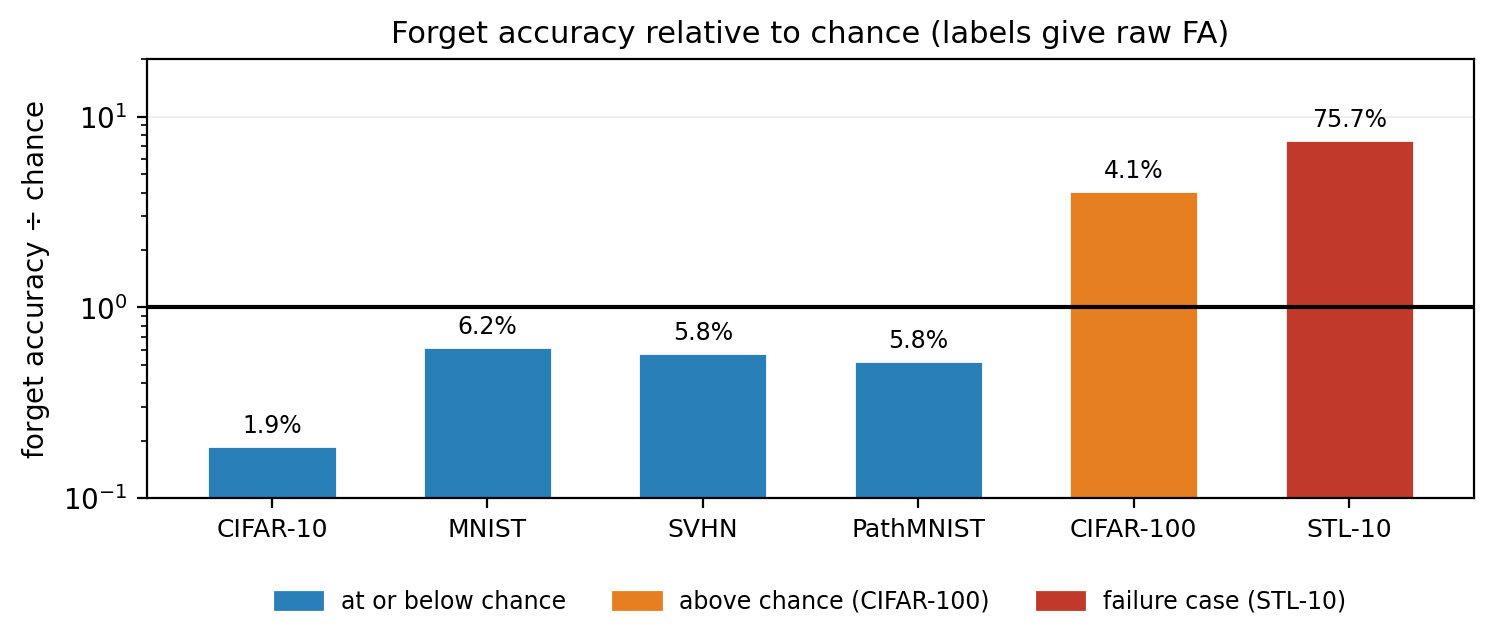
\includegraphics[width=0.86\textwidth]{fig_crossdataset.png}
\caption{\textbf{Forget accuracy relative to the chance level.} Raw forget
accuracy is not comparable across datasets: CIFAR-100's $4.1\%$ is
\emph{above} its $1\%$ chance level while MNIST's $6.2\%$ is \emph{below} its
$10\%$ one. Dividing by $100/K$ puts ``at chance'' at $1.0$ everywhere. Four
datasets sit below chance, CIFAR-100 above it despite a ${\sim}95$pp reduction,
and STL-10 above it at \rev{its 15-epoch cap, though not at 60 epochs}
(\S\ref{sec:crossdataset_stl}).}
\label{fig:crossdataset}
\end{figure}

\paragraph{The projection alone does not unlearn.}
The \emph{projection-only} row is the direct projected-gradient baseline: A-GEM
projection applied to plain gradient ascent, with the KD anchor and the
retain-confusion target removed. It preserves the retain set almost perfectly
($\mathrm{RA} = 99.90\%$), which is what the guarantee promises and all that it
promises---but it stops at $\mathrm{FA} = 18.66\%$, above the $10\%$ chance
level, and halts on the retain-loss budget rather than on the forget target.
Read together with the equal-compute ablation (Table~\ref{tab:ablation}), where
\emph{removing} the projection costs $47.4$pp of retain accuracy, this
delineates the division of labour precisely: the projection supplies retain
safety and nothing else, while the \klr{} objective is what actually drives
forget accuracy to chance. Neither component is sufficient alone, which is the
substantive content of the ablation.

\paragraph{CIFAR-100: scaling to 100 classes.}
Table~\ref{tab:cifar100} gives per-class results (base model TA~$=78.5\%$,
chance $=1\%$). \ours{} reduces FA from ${\sim}99\%$ to a mean of $4.07\%$
(median $1.60\%$) while holding RA at $92.19\%$, with MIA averaging $0.500$.
Eight of nine classes reach FA~$\le 6.8\%$; class~60 is an outlier at $17.8\%$
that does not converge within the 20-epoch budget, and it alone accounts for the
gap between the mean and the median (excluding it, mean FA is $2.35\%$). Unlike
the 10-class datasets, CIFAR-100 does not reach its $1\%$ chance level, so we
report it as a ${\sim}95$pp reduction rather than as forgetting to chance.

\begin{table}[t]
\centering
\caption{\textbf{CIFAR-100 class-level forgetting} (single seed per class,
chance $=1\%$). $^*$Class~60 does not converge within the 20-epoch budget.}
\label{tab:cifar100}
\begin{tabular}{@{}ccccc@{}}
\toprule
Forget class & TA (\%) & FA (\%)$\downarrow$ & RA (\%) & MIA \\
\midrule
10 & 77.23 & 4.20 & 92.84 & 0.485 \\
20 & 76.69 & 1.60 & 92.80 & 0.485 \\
30 & 75.18 & 1.40 & 91.03 & 0.486 \\
40 & 77.19 & 6.80 & 93.14 & 0.506 \\
50 & 76.25 & 0.60 & 92.31 & 0.562 \\
60$^*$ & 76.76 & 17.80 & 92.86 & 0.445 \\
70 & 75.38 & 1.60 & 90.89 & 0.482 \\
80 & 74.95 & 1.00 & 91.51 & 0.553 \\
90 & 75.87 & 1.60 & 92.32 & 0.498 \\
\midrule
\textbf{Mean} & \textbf{76.17} & \textbf{4.07} & \textbf{92.19} & \textbf{0.500} \\
\textbf{Median} & \textbf{76.25} & \textbf{1.60} & \textbf{92.31} & \textbf{0.486} \\
\bottomrule
\end{tabular}
\end{table}

\subsection{Momentum in Detail}\label{app:momentum}

The most direct route to an exact per-step guarantee is to remove momentum, so
that the applied update \emph{is} the projected gradient. Table~\ref{tab:momentum}
shows what that costs. With $\mu=0$ and all else fixed, \ours{} fails to forget
on five of six datasets: FA remains at $95.9\%$ on MNIST, $99.7\%$ on STL-10,
$73.7\%$ on CIFAR-100, and $61.9\%$ on SVHN. Retain accuracy stays high
throughout---but only because the model barely moves; high RA together with high
FA is the signature of a method that preserves retained knowledge by declining
to unlearn.

This is the empirical content of our central methodological claim. A per-step
guarantee stated for the momentum-free update would be exact and
implementation-matched, yet would describe a method that does not unlearn.
Projecting the post-momentum update instead keeps the guarantee exact
\emph{and} recovers forgetting on every dataset where it is attainable.

\begin{figure}[t]
\centering
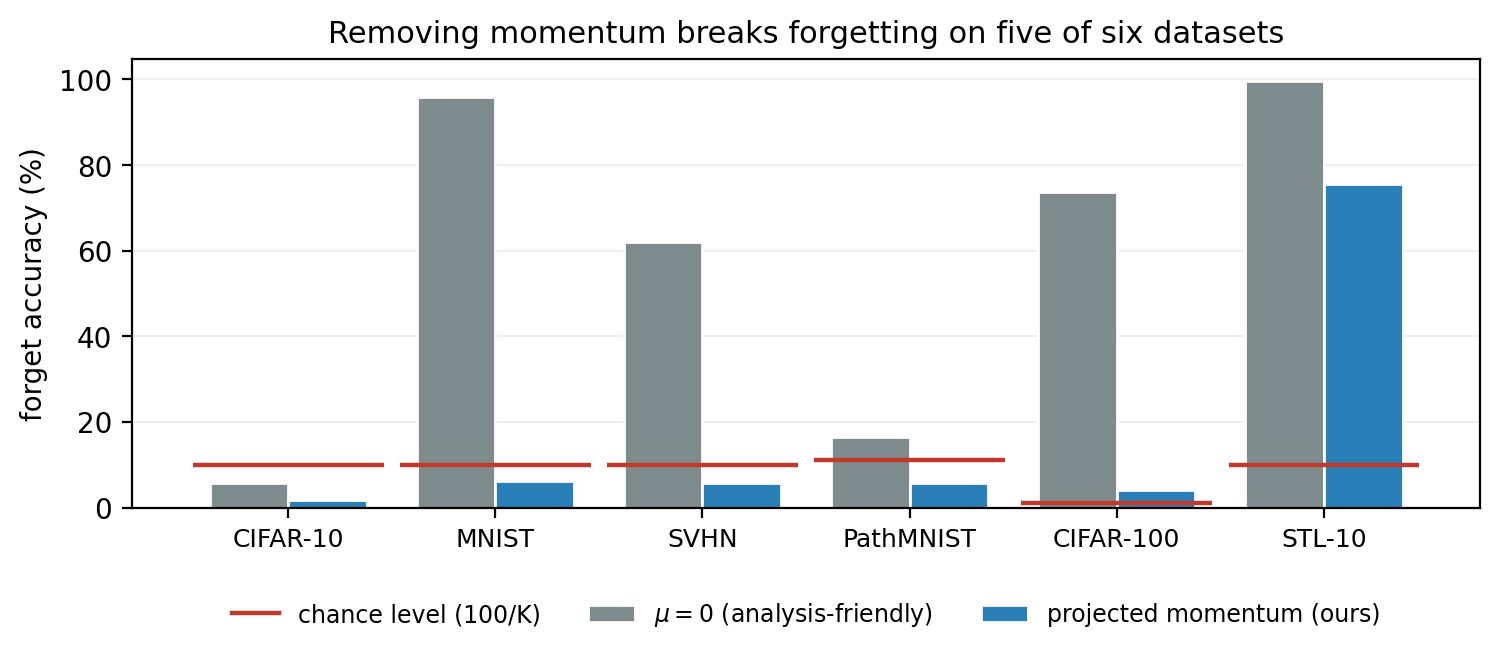
\includegraphics[width=0.86\textwidth]{fig_momentum.png}
\caption{\textbf{Momentum is not incidental.} Forget accuracy with momentum
removed ($\mu=0$, grey) against the projected-momentum update (blue), with each
dataset's chance level in red. The momentum-free configuration---the one for
which an exact guarantee is easiest to state---fails to forget on five of six
datasets. Retain accuracy stays high throughout (Table~\ref{tab:momentum}),
because the model barely moves.}
\label{fig:momentum}
\end{figure}

\paragraph{Is the dependence ours, or the field's?} A natural objection is that
this ablation only tells us something about \ours{}. If every gradient-based
unlearning rule collapses without momentum, the finding is about optimisers and
not about our design; if only ours does, the hard constraint is fragile. We
therefore repeated the ablation across four update rules on the two datasets
where Table~\ref{tab:momentum} shows the largest effect, at \emph{equal compute}
with stopping disabled so that the momentum change is not confounded with step
count (Table~\ref{tab:momentum_rules}).

\begin{table}[t]
\centering
\caption{\textbf{Where the momentum dependence comes from} (equal compute, 12
epochs on MNIST and 15 on SVHN, dual stopping disabled). $\Delta$ is the increase
in forget accuracy when momentum is removed, so larger is more dependent.
Grouping by forget objective separates the rows cleanly; grouping by whether the
projection is used does not.}
\label{tab:momentum_rules}
\begin{tabular}{@{}llcccc@{}}
\toprule
Update rule & Forget objective & Projection & MNIST $\Delta$ & SVHN $\Delta$ & mean \\
\midrule
\ours{}            & $\KL \to p_r$      & yes & $+95.3$ & $+62.4$ & $\mathbf{+78.8}$ \\
\texttt{kl\_uniform} & $\KL \to$ uniform & yes & $+84.9$ & $+56.3$ & $\mathbf{+70.6}$ \\
\addlinespace
projection only    & gradient ascent  & yes & $+16.5$ & $+13.2$ & $+14.8$ \\
gradient ascent    & gradient ascent  & no  & $+11.5$ & $+12.5$ & $+12.0$ \\
\bottomrule
\end{tabular}
\end{table}

Every rule degrades without momentum, including plain gradient ascent, which
uses no projection at all---so the dependence is not an artefact of operating
under a hard per-step constraint. But the rules do not degrade equally, and the
grouping is informative. The two KL-based objectives lose $70$--$79$pp of forget
accuracy on average, the two gradient-ascent objectives $12$--$15$pp: a factor
of $5.6$. Meanwhile the like-for-like comparison that isolates the
projection---gradient ascent with it ($+14.8$) against gradient ascent without
it ($+12.0$)---differs by only $2.8$pp.

The momentum dependence therefore belongs to the \emph{forget objective}, not to
the projection. The reason is visible in the objective itself: $\KL(p_\theta(x_f)
\| p_r)$ is bounded and its gradient vanishes as $p_\theta \to p_r$, so the
per-step signal is small and the $1/(1-\mu) = 10\times$ amplification that
momentum supplies (Lemma~\ref{lem:vel}) is what makes progress possible at
all. Gradient ascent maximises an unbounded loss and needs no such
amplification, which is also why it damages the retained model.

This sharpens rather than weakens the section's claim. The point was never that
momentum is uniquely important to \ours{}; it is that the guarantee must be
stated for the update the optimiser applies, and any method whose objective
requires momentum inherits that requirement. A momentum-free analysis is
convenient for exactly the objectives that cannot afford to be momentum-free.

\subsection{Auditing the Guarantee at Step Level}\label{sec:alignment}

We log every gradient step of a CIFAR-10 class-0 run (120 steps) and check
Theorem~\ref{thm:retain_safety} directly rather than assuming it.

\begin{itemize}
\item \textbf{The constraint is active, not vacuous.} All $120/120$ steps have
$\langle v_t,\gr\rangle < 0$, so the projection fires at every step. Projection
here is not an occasional correction: without it, every step would increase
retain loss to first order.
\item \textbf{The guarantee holds.} After projection,
$\langle u_t,\gr\rangle \ge 0$ at every step to floating-point precision. The
largest relative violation is
$\langle u_t,\gr\rangle/(\|u_t\|\|\gr\|) = -7.4\times 10^{-7}$, against a
float32 accumulation scale of ${\sim}4\times 10^{-4}$ for sums over 11.2M
parameters; the mean relative alignment is positive
($+2.2\times 10^{-8}$). The implied worst-case first-order retain increase is
$3.1\times 10^{-7}$, three orders of magnitude below the observed per-step
retain-loss fluctuation ($1.8\times 10^{-4}$). We therefore state the guarantee
as holding to float32 precision, and recommend float64 accumulation for the
inner products in reference implementations.
\item \textbf{The norm bound is respected.} $\|u_t\|$ reaches a maximum of
$9.16$ against the theoretical bound $c/(1-\mu)=10$, with mean $7.35$---close to
but never exceeding the bound, confirming both that the bound is tight and that
momentum's amplification is being realised.
\item \textbf{Retain loss is controlled.} The mean per-step change in mini-batch
retain CE is $-7.9\times 10^{-5}$ (i.e.\ decreasing), with a maximum single-step
increase of $+1.05\times 10^{-3}$, consistent with the $O(\eta^2)$ term of
Eq.~\ref{eq:thm1}.
\end{itemize}

\subsection{BatchNorm Recalibration in Detail}\label{app:bn}

Table~\ref{tab:gn} reports \ours{} with a GroupNorm backbone across datasets.
GroupNorm keeps forgetting intact on four of five datasets at a modest TA cost
(e.g.\ CIFAR-10 $84.16\%$ vs $86.13\%$), while removing the BN-recalibration
mechanism by construction, since there are no batch statistics to recalibrate.
STL-10 is under-trained under GroupNorm as it is under BN, at \rev{its epoch cap}
(\S\ref{sec:crossdataset_stl}).

\begin{table}[t]
\centering
\caption{\textbf{\ours{} with a GroupNorm backbone} (3-seed means). GroupNorm
removes the BN-recalibration vulnerability structurally. $^*$STL-10 is under-trained under
both backbones.}
\label{tab:gn}
\begin{tabular}{@{}lcccc@{}}
\toprule
\textbf{Dataset} & \textbf{TA} & \textbf{FA}$\downarrow$ & \textbf{RA} & \textbf{MIA} \\
\midrule
CIFAR-10    & 84.16 & 3.44 & 99.23 & 0.478 \\
MNIST       & 90.17 & 5.84 & 99.31 & 0.500 \\
SVHN        & 87.99 & 3.46 & 95.49 & 0.581 \\
STL-10$^*$  & 83.92 & 97.60 & 92.95 & 0.552 \\
PathMNIST   & 72.00 & 2.71 & 95.97 & 0.583 \\
\bottomrule
\end{tabular}
\end{table}

Table~\ref{tab:bnrecal} reports the diagnostic itself. The operator is
\texttt{torch.optim.swa\_utils.update\_bn} applied to the retain set: it resets
every BatchNorm buffer, sets the momentum to \texttt{None} so that PyTorch
accumulates a cumulative rather than exponential average, and runs forward
passes with no backward pass and no weight update. The resulting statistics are
therefore the exact retain-set statistics, independent of the pre-attack buffers
and idempotent in the data. We verify after every run that all learnable
parameters are bit-identical, so nothing but the buffers can have changed. Then
$\Delta F = \mathrm{post} - \mathrm{pre}$ separates weight-level forgetting
($\Delta F \approx 0$) from forgetting mediated by batch statistics
($\Delta F \gg 0$). We also report a weaker variant---forward passes in
\texttt{train} mode under the default exponential average, which is what an
earlier version of this work used---and the two agree to within $1.2$pp on every
row, and to $0.02$pp on the \ours{} row that carries the finding, so the choice
of estimator is not what drives the result. All
accuracies here are measured under deterministic (test-time) transforms; leaving
training augmentation active perturbs individual rows by several points.



\paragraph{The vulnerability is ours, not the field's---in our reproductions.}
The baseline rows matter more than \ours{}'s. Every one of them is unaffected by
recalibration---the largest movement is SCRUB's $-3.6$pp, in the direction of
\emph{more} forgetting---and so is the base model, which is the control that
matters: recalibrating a normally trained network changes nothing, because its
statistics already agree with its weights. Only \ours{} carries a mismatch.
$\Delta F = +98.4$pp means the attack does not merely degrade the unlearning but
\emph{undoes} it: forget accuracy returns to $99.7\%$ and test accuracy to
$92.9\%$\rev{---the values recalibration gives the base model itself ($99.8\%$
and $92.9\%$)}---without a single weight being modified. On a BatchNorm backbone, what \ours{} produces is not an
unlearned model but an unlearned model's statistics.

We qualify the first half of that heading deliberately. \rev{Concurrent work
\citep{kalani2026batchnorm} reports large recoveries for SalUn ($+62.1$pp) and
Bad Teacher ($+78.2$pp) under their reference implementations, where we measure
none. We ran the identical operator, so the disagreement is not in the attack
but in how the unlearned checkpoints were produced. Our implementations end
every epoch with a full pass over retained data in train mode, which recomputes
the running statistics before the checkpoint is saved; \citet{kalani2026batchnorm}
run Bad Teacher's BatchNorm in eval mode, and find that SalUn's recovery
disappears once at least a quarter of each unlearning batch is retained data.}
Our claim is therefore that the vulnerability is \ours{}-specific \emph{among
the checkpoints we trained}, not that these baselines are immune in general.

We attribute it, tentatively, to the interaction between our own design choice
and BatchNorm. \ours{} freezes the normalisation statistics during unlearning so
that class-homogeneous forget batches cannot corrupt them; the weights therefore
adapt against \emph{fixed} statistics, and the resulting decision boundary is
valid only for those statistics. Methods that let the statistics move during
unlearning never build that dependence. Freezing BatchNorm is thus necessary but
not sufficient: it prevents the statistics from manufacturing apparent
forgetting, and simultaneously makes the weights depend on them.
\added{Section~\ref{sec:bn_robust} puts this attribution to an interventional
test: keeping the statistics consistent with the weights throughout unlearning
removes the vulnerability.}

The GroupNorm backbone removes the mechanism by construction---there are no batch
statistics to recalibrate---at a cost of $2.0$pp of test accuracy
(Table~\ref{tab:gn}). The ViT-B/16 backbone
(\S\ref{sec:vit}) does the same for a different reason: LayerNorm normalises
per example at inference and keeps no running statistics either. Two
architectures with unrelated designs are both outside the operator's reach, and
both unlearn properly, which locates the defect in the normalisation scheme
rather than in gradient projection.

We state the limit of that plainly: neither backbone \emph{resists} the attack,
because the attack is undefined on them. This is a design change, not
demonstrated robustness, and a method that must avoid BatchNorm to be safe is
constrained in a way the guarantee itself does not capture. What the two rows do
establish is that the defect is separable from \ours{}'s mechanism---it is a
property of freezing statistics that a normalisation layer keeps, and it
disappears wherever there are no such statistics. \added{The next subsection
removes the constraint itself: it keeps BatchNorm, and makes \ours{} robust to
the attack rather than outside its reach.}

\begingroup\color{revised}% ---- new subsection: everything to \endgroup is added
\subsection{BN-robust \ours{} in Detail}\label{app:bn_robust}

The diagnosis above points at its own remedy: if the weights learn to forget
against statistics that are allowed to go stale, the statistics should never be
stale. BN-robust \ours{} makes three changes to Algorithm~\ref{alg:excise}
(Figure~\ref{fig:bnrobust_mech}). It leaves the update rule untouched, \rev{so
Theorem~\ref{thm:retain_safety} holds at every step for the retain objective
under the statistics in force during that step; the recalibration between steps
is not covered by it}.
\begin{enumerate}
\item \emph{Track the weights.} Before every step the BatchNorm statistics are
recomputed, $\phi \leftarrow R(\theta, B_r)$, with the attacker's own operator
$R$ (\texttt{update\_bn}) on a fresh sample $B_r$ of $512$ retain images. The
step's forward and backward passes then run under statistics consistent with the
current weights. Forget batches still never touch the statistics: this keeps
the half of freezing that was right and drops the half that was wrong.
\item \emph{Ship consistent statistics.} After the last step,
$\phi \leftarrow R(\theta_T, \Dr)$ on the whole retain set under test-time
transforms---exactly what the attacker computes.
\item \emph{Stop on the forget accuracy that ships.} The stopping rule of
\S\ref{sec:stopping} reads FA under $R(\theta, \Dr)$ with test-time transforms,
not under the in-loop statistics. If the target is not met within the epoch
budget, the epoch with the lowest such FA inside the retain budget is shipped
instead of the last one.
\end{enumerate}
\begin{figure}[t]
\centering\color{revised}
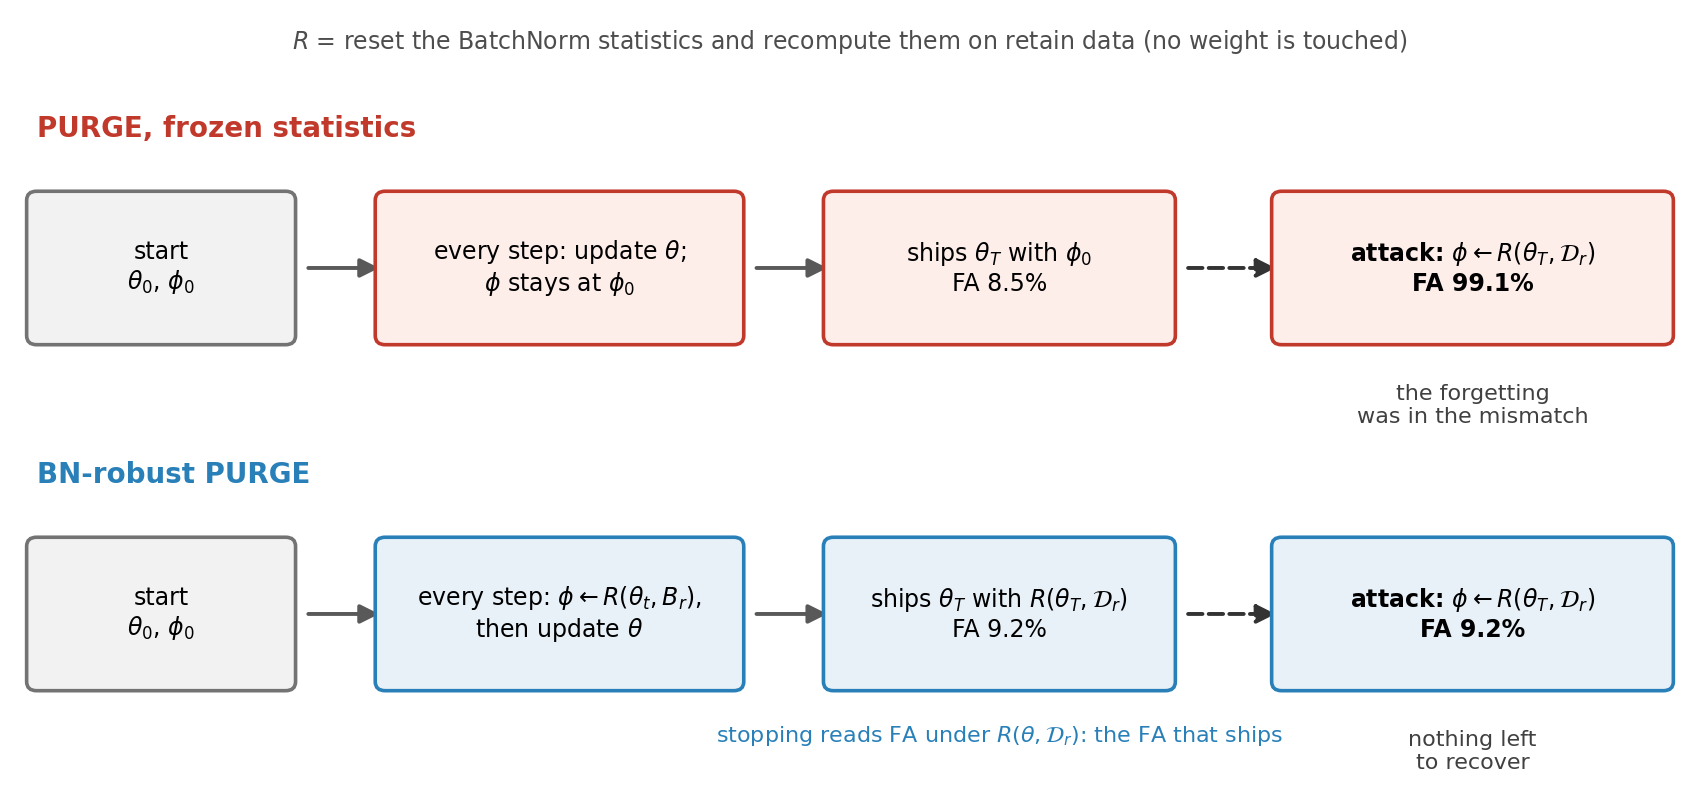
\includegraphics[width=\textwidth]{fig_bnrobust_mechanism.png}
\caption{\added{\textbf{What BN-robust \ours{} changes.} $R$ resets the BatchNorm
statistics and recomputes them on retain data without touching a weight. With
frozen statistics the forgetting lives in the mismatch between $\theta_T$ and
$\phi_0$, and the attack removes it; BN-robust ships statistics consistent with
its weights, so the attack has nothing to recover. Forget accuracies are
CIFAR-10 class~0, means over three seeds (Table~\ref{tab:bnrobust}).}}
\label{fig:bnrobust_mech}
\end{figure}

Because $R$ is idempotent, change~2 makes the attack a no-op on the shipped model
by construction, so $\Delta F = 0$ is not by itself evidence here. The question
this variant must answer is whether FA is still low once $\phi$ cannot be
stale. Two of the tests below are not no-ops by construction: the
exponential-average operator, and recalibration on data other than the retain
set.

Change~3 is not cosmetic. Without it, the FA that triggers stopping is read under
the in-loop statistics---a few hundred augmented images, one step behind---on
augmented forget images. On CIFAR-10 that reading falls short of the shipped FA
by between $-1.0$ and $+9.0$pp depending on the class, and runs stopped at
``FA $\le 10\%$'' shipped at $7.2$--$16.7\%$ (Figure~\ref{fig:bnrobust_stop}). With change~3 the shipped FA meets
the target, and the seed-to-seed spread on class~0 falls from $1.90$ to
$0.08$pp (Table~\ref{tab:bnrobust}). The stopping check need not use the whole
retain set. Computing it on $10{,}240$ images reproduced every stopping decision
of the full check on all three seeds and cut wall-clock by $16\%$; the shipped
statistics still use the full set.

\begin{figure}[t]
\centering\color{revised}
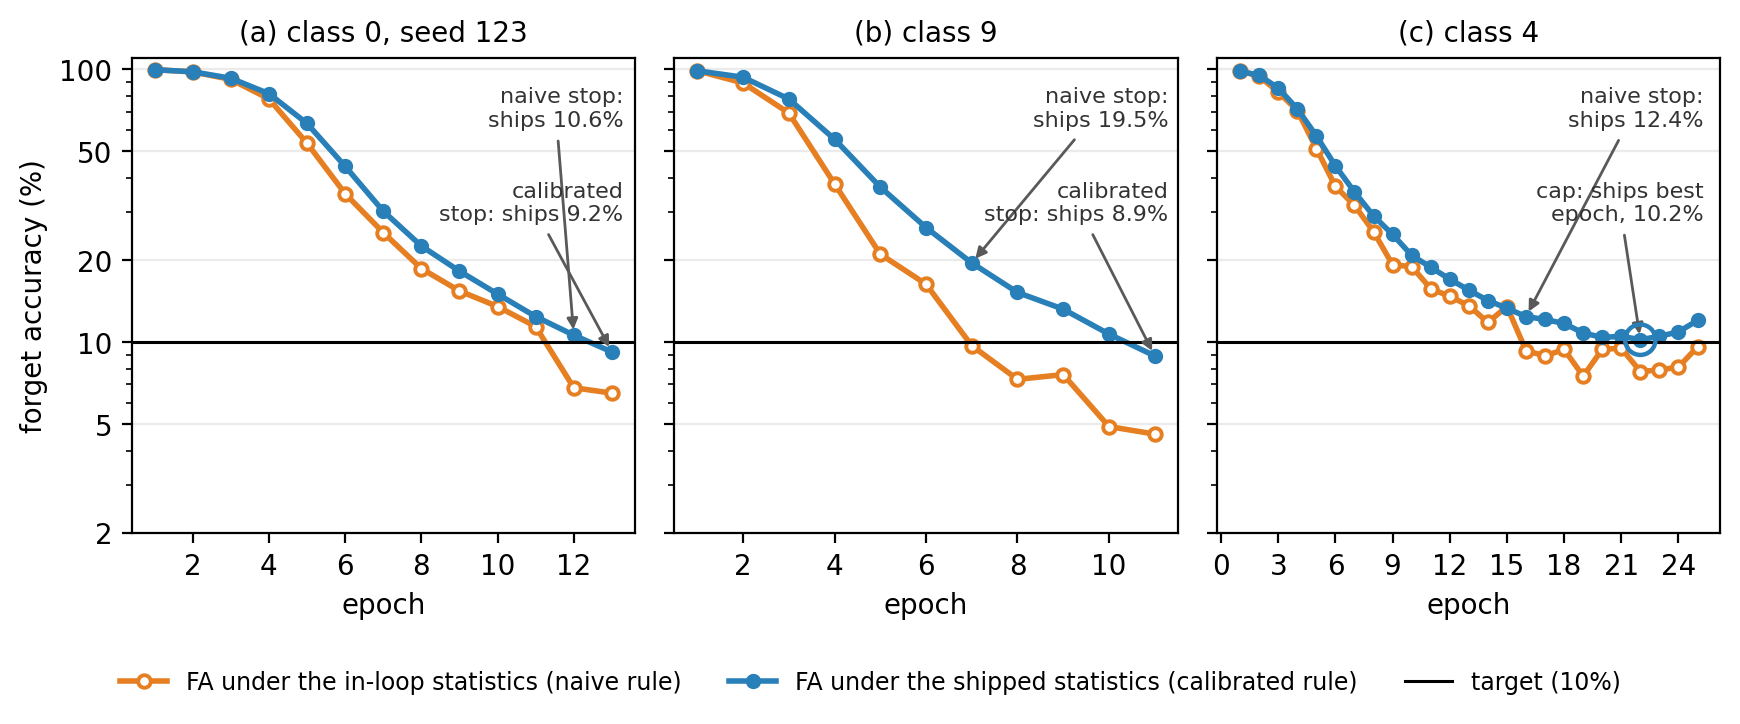
\includegraphics[width=\textwidth]{fig_bnrobust_stopping.png}
\caption{\added{\textbf{Why stopping must be calibrated.} Forget accuracy per epoch
under the in-loop statistics (what naive stopping reads) and under the
statistics that ship (what calibrated stopping reads); log scale. The in-loop
reading runs below the shipped one, so a naive rule stops early and ships above
chance: (a)~one epoch early on class~0, (b)~four epochs early on class~9,
shipping $19.5\%$ instead of $8.9\%$. (c)~On class~4 the shipped FA plateaus just
above $10\%$ and the run reaches the epoch cap; the best-epoch rule ships epoch~22
($10.2\%$) rather than the last ($12.0\%$).}}
\label{fig:bnrobust_stop}
\end{figure}

These experiments were run after the checkpoints behind
Table~\ref{tab:bnrecal} became unavailable. They use an earlier CIFAR-10 base
(test accuracy $93.97\%$, against $95.5\%$ there), a GroupNorm base retrained for
$100$ rather than $200$ epochs ($91.89\%$), and a retrained MNIST base
($99.59\%$). Their absolute numbers are therefore not comparable row for row
with the rest of \S\ref{sec:experiments}; every comparison below is between arms
that share a base.



\paragraph{It survives the attack it was built against, and two it was not.}
Calibrated BN-robust forgets class~0 to $9.19\%$ and stays at $9.18\%$ under
recalibration (Figure~\ref{fig:bnrobust_attack}a), while the frozen configuration
returns to $99.12\%$ with test accuracy back at $94.1\%$---the original model. The exponential-average
operator, which is not idempotent and therefore not a no-op here, moves
BN-robust by at most $+0.3$pp. Nor does robustness depend on the attacker using
the retain set. On the naive-stopping checkpoints, recomputing the statistics
on the full training set, forget class included, or on the test set---data
BN-robust never trained under---moves its FA by $-1.0$ to $-1.2$pp, towards more
forgetting, while the frozen configuration still recovers to $97.4\%$ and
$97.3\%$ (Figure~\ref{fig:bnrobust_attack}b).

\paragraph{Every class, and a second dataset.}
On all ten CIFAR-10 classes (seed~$42$; Table~\ref{tab:app_bnrobust} and
Figure~\ref{fig:app_bnrobust}), the
frozen configuration recovers to $94.7$--$99.3\%$ under the attack, while
BN-robust's FA moves by at most $0.06$pp under either stopping rule. With
calibrated stopping every class ships between $6.7\%$ and $10.2\%$, inside three
standard errors of chance ($11.3\%$ for $5{,}000$ images); with naive stopping,
five of the ten did not. One class needed the fallback. Class~4 hovered at
$10.2$--$10.9\%$ for six epochs without crossing $10\%$ and reached the epoch
cap, and the rule shipped its best epoch ($10.2\%$) rather than the last
($11.9\%$, with retain accuracy $1.4$pp lower). On MNIST, over three seeds, the
frozen configuration's forgetting is undone completely ($0.00\% \to 99.97\%$,
with test accuracy back to $99.56\%$ against the base's $99.59\%$), and
BN-robust holds ($3.78\% \to 3.87\%$, test accuracy $90.10\%$).

\paragraph{What it costs, and why it is slower.}
Against the frozen configuration, BN-robust gives up $1.8$pp of retain accuracy
and $0.9$pp of test accuracy and takes about seven times the wall-clock, most of
it because it needs $13$ epochs instead of $2$. We read the slower forgetting as
the substance rather than the overhead. The frozen configuration reaches its
target in two epochs largely through the statistics mismatch, which the attack
shows is not forgetting at all; once the statistics track the weights, the
forgetting has to happen in the weights. BN-robust's test accuracy, $84.30\%$,
is close to the $84.6\%$ expected from removing one class of ten from a
$93.97\%$ model. Against GroupNorm, BN-robust keeps $1.2$pp more test accuracy,
mostly because it can start from the stronger BatchNorm base, and it needs
neither a change of architecture nor a retrained base model.
Membership-inference AUROC stays between $0.48$ and $0.52$ for every unlearned
row.

\paragraph{What it does and does not establish.}
Unlike GroupNorm or a transformer, this is robustness rather than immunity by
construction: the attack is defined on the model, runs, and finds nothing to
recover. It is robustness to one attack, though. BN-robust changes only how the
normalisation statistics are maintained, so it does nothing against attacks that
modify the weights, such as fine-tuning recovery (\S\ref{sec:limitations}), and
we have tested it on two datasets rather than six. Within that scope, \ours{} no
longer has to choose between BatchNorm and its forgetting: BN-robust \ours{},
\ours{} with GroupNorm, and \ours{} on a transformer are all configurations we
would deploy.
\endgroup% ---- end of the added subsection

\subsection{A Transformer Backbone}\label{sec:vit}

Every result so far uses ResNet-18, so the projection has only ever been applied
to a convolutional network. We repeat CIFAR-10 class~0 on ViT-B/16 under the
identical algorithm, with representation erasure disabled as everywhere else,
over three seeds.

\begin{table}[t]
\centering
\caption{\textbf{ViT-B/16 against ResNet-18}, same algorithm and forget targets
as Table~\ref{tab:cross}\rev{; the ViT runs check forget accuracy every step.
Chance is $10\%$ on CIFAR-10 and $1\%$ on CIFAR-100. The projection fires on
$98$--$100\%$ of steps, as it does on ResNet-18.}}
\label{tab:vit}
\begin{tabular}{@{}lcccc@{}}
\toprule
Backbone & TA & FA$\downarrow$ & RA & MIA \\
\midrule
\multicolumn{5}{@{}l}{\rev{\emph{CIFAR-10, class~0, three seeds}}} \\
ResNet-18 (Table~\ref{tab:cross}) & $86.13 \pm 0.02$ & $1.87 \pm 0.25$ & $100.00 \pm 0.00$ & $0.529$ \\
ViT-B/16                          & $87.05 \pm \rev{0.09}$ & $9.71 \pm \rev{0.27}$ & $\phantom{0}97.55 \pm \rev{0.10}$ & $0.453$ \\
\midrule
\multicolumn{5}{@{}l}{\rev{\emph{CIFAR-100, classes $10,\dots,90$, one seed each, 20-epoch cap}}} \\
\rev{ResNet-18 (Table~\ref{tab:cross})} & \rev{$76.17 \pm 0.86$} & \rev{$4.07 \pm 5.51$} & \rev{$92.19 \pm 0.84$} & \rev{$0.500$} \\
\rev{ViT-B/16} & \rev{$81.97 \pm 0.66$} & \rev{$24.00 \pm 23.16$} & \rev{$91.86 \pm 0.73$} & \rev{$0.435$} \\
\bottomrule
\end{tabular}
\end{table}

\rev{On CIFAR-10} forgetting transfers: FA reaches $9.71\%$, below the $10\%$
chance level, with retain accuracy at $97.55\%$ and test accuracy slightly
\emph{above} the ResNet-18 result. The gap in FA against ResNet-18's $1.87\%$ is not a weaker
result but a different stopping point---both runs use $\tau_F = 10\%$, and
the ViT run halts as soon as it crosses that threshold (epoch~3, mid-epoch),
whereas the ResNet-18 run overshoots it. \S\ref{sec:experiments} shows that
overshoot is an artifact of check granularity rather than a property of either
backbone.

\rev{On CIFAR-100 it does not transfer within the same 20-epoch cap. On the nine
classes of Table~\ref{tab:cross}, ViT-B/16 ends with FA between $4.0\%$ and
$82.0\%$ (mean $24.0\%$) against a $1\%$ chance level, so no class reaches
chance, where ResNet-18 ends at $4.07\%$ and reaches chance at 60 epochs.
Retain accuracy ($91.9\%$) matches ResNet-18's. We have not tested whether a
longer budget closes the gap, as it does for ResNet-18; until then the
transformer result holds for CIFAR-10 only.}

Two things follow. First, the conflict the projection resolves is not an artifact
of convolutional architectures: the projection fires on $99$--$100\%$ of steps
here as well, so forget and retain gradients oppose one another just as
routinely in a transformer. Second, and more usefully,
ViT normalises with LayerNorm, which computes statistics per example at
inference and stores none. It is therefore outside the reach of the
recalibration operator of \S\ref{sec:bn_results} for the same structural reason
as GroupNorm, but by way of a completely different architecture---which is what
makes the pair informative rather than merely repetitive.

\subsection{Component Ablation}\label{sec:ablation}

A component ablation run in the deployed configuration is uninformative here,
and the reason is instructive. Under the projected-momentum optimiser every
variant reaches the forget-accuracy target inside the first check interval, so
dual stopping halts them all after one epoch and each looks equally good: in the
upper half of Table~\ref{tab:ablation}, removing the projection costs
$0.09$pp of retain accuracy. That number is an artefact of stopping, not a
measurement of what the projection does.

We therefore also run every variant at \emph{equal compute}, with stopping
disabled throughout (lower half). The picture inverts.

\begin{table}[t]
\centering
\caption{\textbf{Component ablation} (CIFAR-10 class~0, seed 42). Upper: the
deployed configuration, where dual stopping halts every variant after one epoch.
Lower: equal compute, 15 epochs, stopping disabled for all variants---the same
comparison without the stopping confound. \texttt{+rep} and \texttt{+gate}
re-introduce the two components removed in \S\ref{sec:method}.}
\label{tab:ablation}
\begin{tabular}{@{}llcccc@{}}
\toprule
& Variant & TA & FA & RA & MIA \\
\midrule
\multirow{7}{*}{\rotatebox{90}{\emph{stopping on}}}
 & full \ours{}      & $86.10$ & $2.14$ & $100.00$ & $0.528$ \\
 & $-$KD             & $85.56$ & $0.80$ & $99.99$  & $0.516$ \\
 & $-$projection     & $84.87$ & $0.78$ & $99.91$  & $0.513$ \\
 & selective-layer   & $86.26$ & $3.26$ & $100.00$ & $0.528$ \\
 & $+$rep            & $86.10$ & $2.14$ & $100.00$ & $0.528$ \\
 & $+$gate           & $86.10$ & $2.14$ & $100.00$ & $0.528$ \\
 & $-$stopping       & $85.71$ & $0.00$ & $99.98$  & $0.472$ \\
\midrule
\multirow{6}{*}{\rotatebox{90}{\emph{equal compute}}}
 & full \ours{}      & $85.70$ & $0.00$ & $99.98$  & $0.472$ \\
 & $-$KD             & $85.66$ & $0.00$ & $99.94$  & $0.475$ \\
 & $-$projection     & $\mathbf{44.37}$ & $0.00$ & $\mathbf{52.55}$ & $0.436$ \\
 & selective-layer   & $85.76$ & $0.00$ & $99.99$  & $0.469$ \\
 & $+$rep            & $85.74$ & $0.00$ & $99.98$  & $0.473$ \\
 & $+$gate           & $87.16$ & $19.28$ & $100.00$ & $0.539$ \\
\bottomrule
\end{tabular}
\end{table}

\paragraph{The projection is what makes unlearning survivable.}
At equal compute, removing it costs $41.3$pp of test accuracy and
$47.4$pp of retain accuracy: the model collapses to $44.4/52.6$ against
$85.7/99.98$ for the full method. This is the empirical counterpart of
Theorem~\ref{thm:retain_safety}, and it is a far larger effect than the
stopping-confounded comparison suggests. Note also that the two rows disagree
about the \emph{sign} of the conclusion---one reports the projection as
costless, the other as indispensable---which is why we report both rather than
whichever is more favourable.

\paragraph{KD contributes little once compute is equalised.}
Removing the distillation anchor changes retain accuracy by $0.04$pp at equal
compute. We previously attributed several points of retain accuracy to it; that
is not supported here, and we no longer claim it.

\paragraph{The removed components stay removed.}
Re-introducing representation erasure reproduces the full method to within
$0.04$pp on every metric, and re-introducing the entropy gate leaves forget
accuracy at $19.3\%$---above the $10\%$ chance level, i.e.\ it prevents the
method from forgetting. Both were dropped in \S\ref{sec:method} on the strength
of an ablation run under the previous implementation; this re-run confirms the
decision under the current one.

\subsection{How Hard Must the Constraint Be?}\label{sec:strength}

Theorem~\ref{thm:separation}(iv) argues that a soft conflict penalty biases the
update without excluding retain-harming steps, and that only a hard constraint
makes them unreachable. That is an argument about feasible sets; here we measure
what it costs in practice. We interpolate the projection with a strength
parameter $s$: at each conflicting step the update becomes
$u_t = v_t - s\,\frac{\langle v_t,\gr\rangle}{\|\gr\|^2}\gr$, so
\begin{equation}\label{eq:strength}
\langle u_t, \gr\rangle \;=\; (1-s)\,\langle v_t, \gr\rangle .
\end{equation}
At $s=0$ nothing is corrected; at $s=1$ this is \ours{}. Every intermediate
value is a soft penalty---it shrinks the conflicting component without removing
it---and by Eq.~\ref{eq:strength} it leaves $\langle u_t,\gr\rangle<0$ whenever
the raw update conflicts. All other settings are held fixed, and stopping is
disabled so that every variant sees the same compute.

\begin{table}[t]
\centering
\caption{\textbf{Projection strength} (CIFAR-10 class~0, equal compute, stopping
disabled). $s=0$ applies no correction, $s=1$ is the full hard constraint.
Forget accuracy is $0.0\%$ throughout, so the runs differ only in collateral
damage.}
\label{tab:strength}
\begin{tabular}{@{}lccccc@{}}
\toprule
$s$ & residual conflict & TA & FA & RA & MIA \\
\midrule
$0.00$ & $1.00\,\langle v_t,\gr\rangle$ & $44.35$ & $0.0$ & $52.54$ & $0.436$ \\
$0.25$ & $0.75\,\langle v_t,\gr\rangle$ & $67.84$ & $0.0$ & $81.35$ & $0.497$ \\
$0.50$ & $0.50\,\langle v_t,\gr\rangle$ & $78.03$ & $0.0$ & $92.75$ & $0.510$ \\
$0.75$ & $0.25\,\langle v_t,\gr\rangle$ & $82.99$ & $0.0$ & $98.24$ & $0.509$ \\
$1.00$ & $\mathbf{0}$ & $\mathbf{85.71}$ & $0.0$ & $\mathbf{99.98}$ & $0.472$ \\
\bottomrule
\end{tabular}
\end{table}

\begin{figure}[t]
\centering
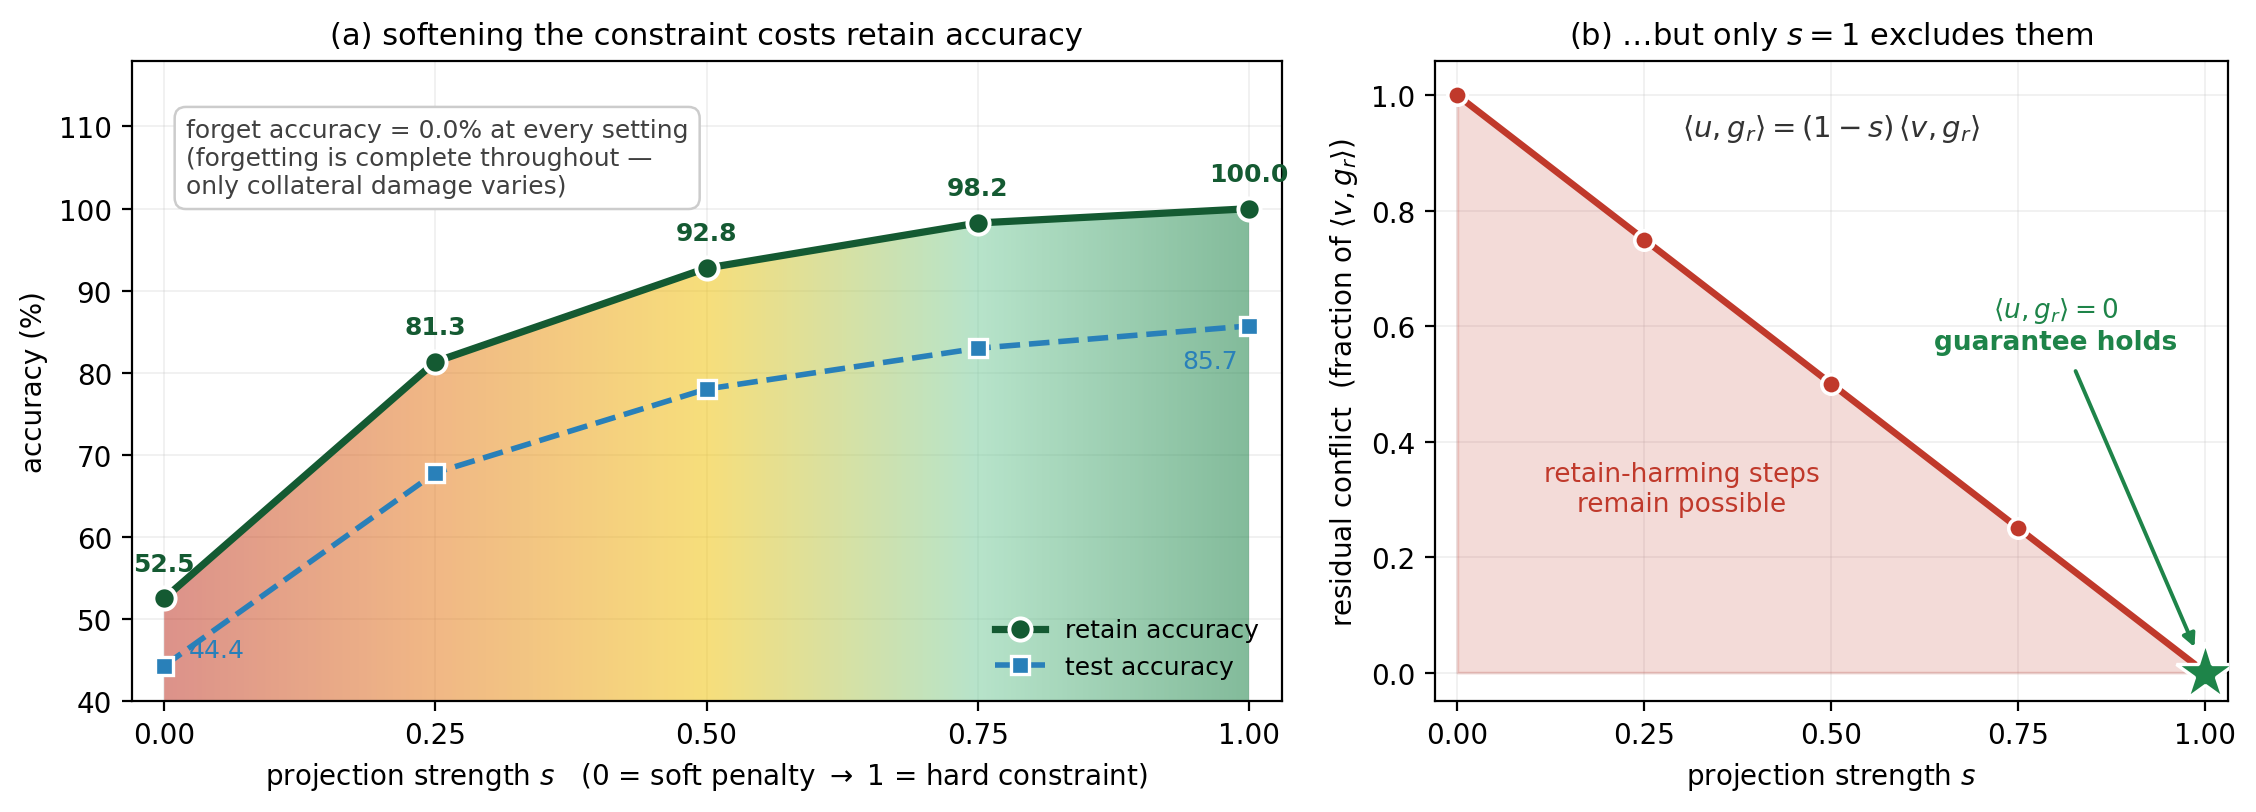
\includegraphics[width=\textwidth]{fig_strength.png}
\caption{\textbf{Hardening the constraint recovers retain accuracy
continuously, but only the endpoint carries the guarantee.}
\textbf{(a)}~Retain and test accuracy against projection strength; forget
accuracy is $0.0\%$ at every setting, so the runs differ only in collateral
damage. \textbf{(b)}~Residual conflict $(1-s)$: retain-harming steps remain
reachable for every $s<1$ and are excluded only at $s=1$. The empirical
difference between $s=0.75$ and $s=1$ is $1.7$pp of retain accuracy; the
difference in what can be proved is categorical.}
\label{fig:strength}
\end{figure}

\paragraph{Softening is expensive, and monotonically so.}
Retain accuracy falls from $99.98\%$ at $s=1$ to $52.54\%$ at $s=0$, and test
accuracy from $85.71\%$ to $44.35\%$, monotonically in between. Because forget
accuracy is $0.0\%$ at every setting, this is not a privacy--utility trade-off:
all five runs forget equally, and they differ only in how much of the retained
model they destroy on the way. The $s=0$ row reproduces the equal-compute
$-$projection ablation of Table~\ref{tab:ablation} from an independent
direction.

\paragraph{The curve is gradual, which we take as a limitation of the empirical
argument.} Most of the benefit arrives early---$s=0.25$ already recovers
$28.8$pp of retain accuracy, while the final quarter, $s=0.75\to1$, is worth
$1.7$pp. A soft penalty tuned near $s=0.75$ therefore performs almost as well as
the hard constraint on these metrics, and we do not claim otherwise. What it
does not do is satisfy Eq.~\ref{eq:strength} with equality: at $s=0.75$ a
quarter of every conflict survives into the applied update, so
$\langle u_t,\gr\rangle<0$ on conflicting steps and no per-step statement can be
made. The case for $s=1$ is therefore not that the last $1.7$pp is large, but
that it is the only setting about which anything can be proved---which is the
whole content of Theorem~\ref{thm:retain_safety}.

\paragraph{Relation to soft conflict-resolution methods.}
This is a controlled test of the mechanism that separates \ours{} from the
closest prior work \citep{patel2025learning}, not a comparison with that method:
it varies our own projection rather than reimplementing theirs, and their
penalty acts on the objective rather than on the update. What it establishes is
the general shape of the trade---that discouraging conflict helps in proportion
to how much of it is removed, and that removing all of it is what converts an
empirical tendency into a guarantee. A like-for-like comparison remains future
work (\S\ref{sec:limitations}).

\subsection{Privacy--Utility Frontier and Robustness Diagnostics}\label{sec:sweeps}

We sweep the two tolerances of Eq.~\ref{eq:problem} independently on CIFAR-10
class~0 (Table~\ref{tab:sweeps}). The results are asymmetric: one tolerance is
inert because the projection has already done its work, while the other is
genuinely active but was hidden by how coarsely we measured it.

\begin{table}[t]
\centering
\caption{\textbf{Tolerance sweeps} (CIFAR-10 class~0). Sweep~A varies the
retain-loss budget $\alpha$ at fixed $\tau_F = 10\%$; Sweeps~B and B$'$ vary
the forget-accuracy target $\tau_F$ at fixed $\alpha = 5$, checking forget
accuracy every 50 batches and every step respectively. $\alpha$ is inert. So is
$\tau_F$ under the coarse check---but only because forget accuracy crosses
the whole range between two consecutive checks; measured per step, it tracks the
requested tolerance across a $29$pp range.}
\label{tab:sweeps}
\begin{tabular}{@{}lccccc@{}}
\toprule
\multicolumn{2}{@{}l}{Sweep A: $\alpha$} & TA & FA & RA & MIA \\
\midrule
& $1.5$    & $86.10$ & $1.88$ & $100.00$ & $0.530$ \\
& $2$      & $86.10$ & $1.88$ & $100.00$ & $0.530$ \\
& $3$      & $86.10$ & $1.88$ & $100.00$ & $0.530$ \\
& $5$      & $86.10$ & $1.88$ & $100.00$ & $0.530$ \\
& $10$     & $86.10$ & $1.88$ & $100.00$ & $0.530$ \\
& $9999$   & $86.10$ & $1.88$ & $100.00$ & $0.530$ \\
\midrule
\multicolumn{2}{@{}l}{Sweep B: $\tau_F$, check every 50 batches} & TA & FA & RA & MIA \\
\midrule
& $1\%$    & $85.75$ & $\phantom{0}0.28$ & $100.00$ & $0.521$ \\
& $5\%$    & $86.10$ & $\phantom{0}1.88$ & $100.00$ & $0.530$ \\
& $10\%$   & $86.10$ & $\phantom{0}1.88$ & $100.00$ & $0.530$ \\
& $20\%$   & $86.10$ & $\phantom{0}1.88$ & $100.00$ & $0.530$ \\
& $30\%$   & $86.10$ & $\phantom{0}1.88$ & $100.00$ & $0.530$ \\
\midrule
\multicolumn{2}{@{}l}{Sweep B$'$: $\tau_F$, check every step} & TA & FA & RA & MIA \\
\midrule
& $1\%$    & $85.95$ & $\phantom{0}\mathbf{0.60}$ & $100.00$ & $0.531$ \\
& $5\%$    & $86.34$ & $\phantom{0}\mathbf{3.86}$ & $100.00$ & $0.528$ \\
& $10\%$   & $86.59$ & $\phantom{0}\mathbf{8.24}$ & $100.00$ & $0.522$ \\
& $20\%$   & $87.22$ & $\mathbf{16.24}$ & $100.00$ & $0.518$ \\
& $30\%$   & $88.10$ & $\mathbf{29.60}$ & $100.00$ & $0.515$ \\
\bottomrule
\end{tabular}
\end{table}

\paragraph{The retain budget is non-binding.}
Varying $\alpha$ over four orders of magnitude changes nothing: the retain-loss
constraint is never the active one, because the projection already prevents the
retain loss from rising. This is consistent with Theorem~\ref{thm:retain_safety}
and means $\alpha$ can be left at its default.

\paragraph{The forget target is a usable knob, but only if it is measured
finely enough.} Sweep~B contains no frontier: every target from $5\%$ to $30\%$
yields the identical operating point, $\mathrm{FA} = 1.88\%$. We previously read
this as evidence that $\tau_F$ is not a knob at all. That reading was wrong,
and Sweep~B$'$ shows why: the sweep was limited by the \emph{measurement}, not
by the method.

Forget accuracy is checked every 50 batches, and under this optimiser it falls
from ${\sim}99\%$ to below $2\%$ inside a single such interval, so every target
in between is passed unobserved and the run halts at whichever point the next
check happens to catch. Sweep~B$'$ repeats the sweep with the check evaluated at
every step---on a subsample of $\Df$, with any trigger confirmed on the full
forget set before stopping---and the frontier appears: forget accuracy tracks
the requested tolerance monotonically from $0.60\%$ to $29.60\%$, a $29$pp
range, with test accuracy rising from $85.95\%$ to $88.10\%$ as the tolerance is
relaxed and retain accuracy pinned at $100.00\%$ throughout. At
$\tau_F = 30\%$ the coarse check lands at $\mathrm{FA} = 1.88\%$ where
$29.60\%$ was reachable: a $27.5$pp overshoot attributable entirely to
measurement granularity.

Step-level traces confirm that nothing about the collapse forbids resolving it.
The largest single-step change in forget accuracy is $11.7$--$11.9$pp across
the five targets---the runs follow one trajectory and differ only in where they
leave it. A $12$pp-per-step descent is comfortably resolvable at
per-step granularity; it was invisible at 50-batch granularity. We therefore
restore the $\tau_F$ entry in Table~\ref{tab:properties}, with the
qualification that the tolerance is honoured only when the stopping rule is
evaluated at a resolution finer than the descent it is meant to catch. The cost
is one forward pass over a $512$-sample subsample per step.

\paragraph{MIA in isolation is uninformative.}
An early sign of this: the \emph{pre-unlearning} base model already attains MIA
AUROC $=0.533$ at FA~$=99.7\%$. For well-generalising classifiers, per-sample
membership carries little signal at the class level, so MIA AUROC alone cannot
certify class-level unlearning and must be paired with FA. \S\ref{sec:mia}
develops this into a sharper statement: under the standard protocol the attack
scores \emph{higher} against a model that never saw the data than against one
that memorised it.

\subsection{Distance to a Retrained Model}\label{sec:distance}

Forget accuracy asks whether the forget class is still predicted. It does not
ask whether the unlearned model \emph{behaves like} one trained without that
class, which is what unlearning is for. We therefore retrain a CIFAR-10
reference from scratch on the retain set only, keeping all $K$ output heads so
that output distributions remain comparable, and measure how far each unlearned
model sits from it (Table~\ref{tab:distance}). Two spaces are measured: the
output distribution on forget-class inputs (Jensen--Shannon divergence, and
top-1 agreement with the reference's predictions), and the penultimate feature
distribution (Fr\'echet distance).

\begin{table}[t]
\centering
\caption{\textbf{Distance to a retrained CIFAR-10 reference} (class~0). The
reference is trained on the retain set only. JS and agreement compare output
distributions on forget-class inputs; Fr\'echet compares penultimate features.
Best per column in bold. Parameter distance is reported for completeness only
(see text).}
\label{tab:distance}
\begin{tabular}{@{}lccccccc@{}}
\toprule
Method & JS$\downarrow$ & agree \%$\uparrow$ & Fr\'echet$\downarrow$ &
$\|\Delta\theta\|_2$ & FA & RA & $|\mathrm{MIA}{-}0.5|\downarrow$ \\
\midrule
SalUn        & $\mathbf{0.220}$ & $\mathbf{56.5}$ & $495.3$ & $80.6$ & $0.00$  & $97.70$ & $0.075$ \\
Bad Teacher  & $0.263$ & $47.1$ & $153.0$ & $89.7$ & $24.36$ & $89.46$ & $\mathbf{0.029}$ \\
SCRUB        & $0.562$ & $\phantom{0}8.7$ & $165.9$ & $56.6$ & $89.28$ & $97.83$ & $0.030$ \\
\midrule
\ours{}      & $0.273$ & $35.2$ & $\mathbf{13.0}$ & $43.2$ & $\phantom{0}1.76$ & $\mathbf{100.00}$ & $0.030$ \\
\bottomrule
\end{tabular}
\end{table}

\paragraph{The two spaces disagree, and no method dominates.}
\ours{} is closest to the reference in feature space by a wide margin---a
Fr\'echet distance of $13.0$ against $153$--$495$ for the baselines, a factor of
$38$ against SalUn---and it is the only method that leaves retain accuracy
untouched. SalUn is closest in output space, with the lowest JS divergence
($0.220$ against our $0.273$) and the highest agreement with the reference's
predictions on forget inputs ($56.5\%$ against our $35.2\%$). We report this
plainly: on the metric that most directly operationalises ``behaves like a
retrained model'' on forget inputs, \ours{} is second.

The disagreement is itself the finding. A method can route forget-class inputs
much as a retrained model would while carrying internal representations far from
it, or preserve those representations while routing inputs differently. Reporting
a single distance would have concealed this, and which number one reports would
have determined which method appeared better. We therefore recommend that
distance-to-retrained be reported in both spaces, and we do so.

\paragraph{SCRUB is far away because it has not unlearned.}
Its JS divergence is more than twice ours and its agreement with the reference
is $8.7\%$, but this follows from $\mathrm{FA} = 89.3\%$: a model that still
classifies the forget class correctly cannot resemble one that never saw it.
This is a useful sanity check on the metric---it ranks non-unlearning last---%
rather than a criticism of SCRUB under a different operating point.

\paragraph{Parameter distance is uninformative.}
$\|\Delta\theta\|_2$ orders the methods differently again ($43.2$ for \ours{},
$56.6$ for SCRUB, $80.6$ for SalUn, $89.7$ for Bad Teacher) and tracks neither
behavioural measure. Permutation and scaling symmetries mean two functionally
identical networks can sit far apart in parameter space, so we report it for
completeness and draw no conclusion from it.

\subsection{Membership Inference, Recalibrated}\label{sec:mia}

Every MIA number reported so far, in this paper and in much of the unlearning
literature, is read against a target of $0.5$: the attack should be unable to
distinguish forget-class training samples from forget-class test samples. We ran
four attacks against a retrained reference to check that target, and it does not
survive.

We evaluate four threshold-free signals---negative loss, maximum confidence,
negative entropy, and modified entropy \citep{song2021systematic}, the last of
which uses the true label and so separates confidently-correct from
confidently-wrong predictions---and report AUROC together with true-positive
rate at $1\%$ false-positive rate. The second matters because an attack that
identifies a few members with near-certainty is a real privacy failure that an
average AUROC of $0.5$ can conceal.

\begin{table}[t]
\centering
\caption{\textbf{MIA suite on CIFAR-10 (class~0).} Members are forget-class
training samples, non-members forget-class test samples ($5000$ vs $1000$). The
retrained reference trained on \emph{neither} group, so it is the empirical
target; the base model trained on the members and is the opposite anchor.
TPR is at $1\%$ FPR.}
\label{tab:mia}
\begin{tabular}{@{}lcccccccc@{}}
\toprule
& & \multicolumn{2}{c}{loss} & \multicolumn{2}{c}{mentr} &
\multicolumn{2}{c}{conf} & entropy \\
\cmidrule(lr){3-4}\cmidrule(lr){5-6}\cmidrule(lr){7-8}\cmidrule(lr){9-9}
Model & FA & AUROC & TPR & AUROC & TPR & AUROC & TPR & AUROC \\
\midrule
retrained (reference) & $0.0$  & $0.694$ & $12.5\%$ & $0.646$ & $9.9\%$ & $0.435$ & $0.1\%$ & $0.422$ \\
base (no unlearning)  & $100.0$ & $0.483$ & $0.0\%$  & $0.486$ & $0.0\%$ & $0.482$ & $0.0\%$ & $0.479$ \\
\midrule
SalUn                 & $0.0$   & $0.500$ & $0.0\%$  & $0.537$ & $2.3\%$ & $0.463$ & $0.0\%$ & $0.461$ \\
Bad Teacher           & $24.8$  & $0.485$ & $0.2\%$  & $0.493$ & $0.2\%$ & $0.455$ & $0.6\%$ & $0.444$ \\
SCRUB                 & $89.5$  & $0.477$ & $0.4\%$  & $0.478$ & $0.4\%$ & $0.467$ & $0.4\%$ & $0.462$ \\
\ours{}               & $2.0$   & $0.693$ & $1.4\%$  & $0.691$ & $1.3\%$ & $0.369$ & $0.0\%$ & $0.340$ \\
\bottomrule
\end{tabular}
\end{table}

\paragraph{The retrained reference does not score $0.5$.}
It scores $0.694$ on the loss attack, with a true-positive rate of $12.5\%$ at
$1\%$ false positives. This model trained on \emph{neither} group: to it, forget
train and forget test are both non-members. The attack is therefore not
detecting membership. It is detecting that the CIFAR-10 train and test splits of
class~0 differ in difficulty, and that difference is visible through any model
that has not memorised either. A target of $0.5$ is wrong for this protocol, and
$0.694$ is the level a perfectly unlearned model actually exhibits.

\paragraph{The attack works \emph{better} against the model that never saw the
data.} The base model memorised all $5000$ members and classifies them at
$100\%$; the standard intuition says it should be the most attackable thing in
the table. It scores $0.483$---below chance, and $0.21$ below the retrained
reference. A well-generalising classifier treats members and non-members of a
class alike, leaving no signal, whereas a model that never saw the class makes
errors whose pattern differs between the splits. Under this protocol, MIA AUROC
is anti-correlated with memorisation.

\paragraph{The choice of target reverses the ranking.}
Read against $0.5$, \ours{} looks like the \emph{worst} method in the table
($|{\rm AUROC}-0.5| = 0.193$) and SalUn like the best ($0.000$). Read against the
retrained reference---the model unlearning is supposed to imitate---the order
inverts: \ours{} is nearest ($|{\rm AUROC}-{\rm ref}| = 0.001$) and SalUn is
$0.194$ away. We report both columns rather than the flattering one, and we note
that our own earlier claim of ``MIA within $0.035$ of the ideal $0.5$'' was
resting on the wrong reference point.

We do not want to over-read the agreement between \ours{} and the reference. It
is one dataset, one forgotten class, one protocol, and matching to $0.001$ is
closer than the measurement warrants; what the data supports is that \ours{}
sits near the retrained model on this attack while the baselines sit near $0.5$,
not that it matches it exactly.

\paragraph{On a second dataset the reference is not even a \emph{constant}.}
The argument above rests on one dataset and one class, which is thin for a claim
about everyone's protocol, so we repeated it on PathMNIST, retraining a
reference for each of four classes (Table~\ref{tab:mia_path}). The finding is
sharper than we expected. The reference AUROC is not merely different from
$0.5$; it moves with the forgotten class, and by a large amount. On the loss
attack it ranges from $0.306$ (class~2) to $0.704$ (class~0), a span of
$0.398$---wider than the entire distance from $0.5$ to either endpoint. The
other three attacks span $0.31$--$0.36$ similarly, and reverse direction: on
class~0 the reference sits \emph{above} $0.5$ for loss and \emph{below} it for
confidence, while on classes 2--4 that ordering flips.

\begin{table}[t]
\centering
\caption{\textbf{MIA on PathMNIST, four classes, each against its own retrained
reference.} The reference is the level a perfectly unlearned model exhibits.
There is no single such level: it depends on which class was forgotten, and the
attacks disagree on direction. Gap is the mean over the four attacks of
$|\mathrm{AUROC}_{\ours{}} - \mathrm{AUROC}_{\mathrm{ref}}|$.}
\label{tab:mia_path}
\begin{tabular}{@{}llccccc@{}}
\toprule
Class & Model & loss & mentr & conf & entropy & gap \\
\midrule
\multirow{2}{*}{0} & retrained (reference) & $0.704$ & $0.684$ & $0.345$ & $0.344$ & --- \\
                   & \ours{}               & $0.711$ & $0.719$ & $0.305$ & $0.267$ & $\mathbf{0.040}$ \\
\addlinespace
\multirow{2}{*}{2} & retrained (reference) & $0.306$ & $0.360$ & $0.563$ & $0.571$ & --- \\
                   & \ours{}               & $0.403$ & $0.407$ & $0.187$ & $0.141$ & $0.237$ \\
\addlinespace
\multirow{2}{*}{3} & retrained (reference) & $0.345$ & $0.329$ & $0.666$ & $0.657$ & --- \\
                   & \ours{}               & $0.569$ & $0.597$ & $0.201$ & $0.180$ & $0.359$ \\
\addlinespace
\multirow{2}{*}{4} & retrained (reference) & $0.359$ & $0.366$ & $0.614$ & $0.617$ & --- \\
                   & \ours{}               & $0.589$ & $0.598$ & $0.412$ & $0.410$ & $0.218$ \\
\midrule
\multicolumn{2}{@{}l}{reference range across classes} & $0.398$ & $0.355$ & $0.321$ & $0.312$ & \\
\bottomrule
\end{tabular}
\end{table}

This strengthens the diagnosis considerably. It is not that the field uses the
wrong constant; it is that no constant is correct. Any protocol that scores
unlearning by $|\mathrm{AUROC} - 0.5|$ is comparing against a quantity that
varies by up to $0.4$ with the choice of forgotten class, so the same method can
be judged excellent or poor on the same dataset depending on which class the
deletion request happens to name.

\paragraph{Our own matching result does not generalise, and we withdraw the
general form of it.} The CIFAR-10 agreement above ($0.001$ on the loss attack)
is not reproduced on PathMNIST. \ours{} matches its class-0 reference closely
(mean gap $0.040$, comparable to CIFAR-10's $0.049$), but on classes 2, 3 and~4
the mean gaps are $0.237$, $0.359$ and $0.218$---an average of $0.213$ across
the four classes, four times the CIFAR-10 figure. \ours{}'s own AUROC is
comparatively stable across classes while the reference is not, so the method
does not track a moving target.

We therefore restrict the claim: on CIFAR-10, and on the class of PathMNIST
where the reference resembles CIFAR-10's, \ours{} sits close to the retrained
model on loss-based attacks; we do not claim this holds across forgotten classes
in general, and the PathMNIST measurements show that it does not. The protocol
finding and the method finding should be read separately---the first is
strengthened by this experiment, and the second is narrowed by it.

\paragraph{An AUROC of exactly $0.5$ can be degenerate.}
SalUn's loss attack gives $0.5000$ with a true-positive rate of $0.0\%$ at every
false-positive rate we measured. An uninformative-but-varying score gives
TPR~$\approx$~FPR, i.e.\ about $1\%$; a TPR of zero is the signature of a
\emph{constant} score. SalUn maps every forget-class input to the same output,
so there is nothing for the attack to rank. This is a way of being unattackable,
but it is not evidence of having imitated a retrained model---and reporting
AUROC alone cannot tell the two apart. The TPR column can.

\paragraph{Recommendation.}
For class-level unlearning we recommend that MIA be reported (i)~with more than
one attack, since the four disagree here even in sign---the reference is above
$0.5$ on loss and below it on confidence, and that ordering itself flips between
PathMNIST classes; (ii)~with TPR at a low FPR alongside AUROC, since an AUROC of
$0.5$ can be produced by a constant score that no attack can rank;
(iii)~calibrated against a retrained reference rather than against $0.5$; and
(iv)~\emph{per forgotten class}, against that class's own reference, because
Table~\ref{tab:mia_path} shows a single reference does not transfer between
classes of one dataset.

Point~(iv) is expensive---it costs one retraining per class---which is the
honest obstacle to the recommendation. Where that is out of reach, we would
report MIA as a diagnostic alongside forget accuracy and decline to draw any
conclusion from its distance to $0.5$, rather than treat $0.5$ as a target the
measurements do not support.

\subsection{Over-Forgetting, and a Fix That Did Not Work}\label{sec:overforget}

Two PathMNIST classes are over-forgotten: MIA AUROC reaches $0.298$ and $0.388$,
i.e.\ forget-class training samples become \emph{harder} to classify than
forget-class test samples. Such a model is still distinguishable from a
retrained one---in the opposite direction to a privacy leak---while satisfying
every forget-accuracy check. FA cannot detect this, because moving \emph{to} the
distribution a retrained model produces and moving \emph{past} it both give
$\mathrm{FA}\approx 0$.

We hypothesised that the cause was the gap between stating the forget-side
condition on distributions, \rev{$\KL(p_\theta(x_f)\|p_r)\le\epsilon$---as an
earlier version of Eq.~\ref{eq:problem} did---and implementing it on the
argmax, $\mathrm{FA}\le\tau_F$, as dual stopping does}, and that stopping on the
divergence instead would fix it. We retrained reference models
without the forget class, pre-committed to the prediction, and ran the
experiment. \textbf{The prediction failed.} Stopping on the divergence was worse
on 10 of 12 comparisons, made Jensen--Shannon divergence to the retrained
reference worse on all three classes, and degraded an unaffected control
class---the signature that rules out a targeted fix. Across checkpoints the
proposed criterion is rank-\emph{anti}-correlated with distance to the retrained
model ($\rho=-1.00$): driving it toward zero moves the model away from the
reference. Appendix~\ref{app:d2r} reports the experiment in full, including a
limitation of the test itself and a confound we cannot separate.

Two conclusions follow, and we adopt both. First, a narrower reading of the
\klr{} objective: $p_r$ is a useful forget-side \emph{direction}
(\S\ref{sec:forget_obj}), but it is not what a retrained model produces on
forget inputs, and minimising the divergence to it is actively harmful.
\rev{This is why Eq.~\ref{eq:problem} states the forget condition as a target
met at the end of the search, with the divergence only as its direction, rather
than as an objective to be driven to its minimum.} Second, the
experiment localised a different and more mundane cause: all three FA-stopped
runs overshoot their own $11.1\%$ target by ${\sim}4$pp because the intra-epoch
FA check is evaluated only every 50 batches, and divergence to the retrained
model is lower at the earlier stopping point in every class. The indicated fix
is to stop earlier and more precisely rather than to replace the stopped
quantity.

That fix is now implemented and it works. Evaluating the check at every step
rather than every 50 batches removes the overshoot on CIFAR-10 and recovers a
monotonic frontier over a $29$pp range of forget accuracy
(\S\ref{sec:experiments}, Sweep~B$'$ of Table~\ref{tab:sweeps}); the descent it
must resolve is ${\sim}12$pp per step, which is well within reach at that
granularity. The mechanism is shared, so we expect the same remedy to reduce the
PathMNIST overshoot, but we have not re-run the over-forgotten classes under the
finer check and do not claim the over-forgetting defect itself is resolved. What
has changed is its status: it is a consequence of measuring the stopping
criterion too coarsely, not evidence that the criterion is the wrong one. The
remaining question---where along the trajectory divergence to the retrained
model is minimised, and whether a single FA level identifies it across
classes---stays open.

\subsection{Locating the Stopping Point, and What MIA Cannot Tell Us}
\label{sec:trajectory}

The refuted hypothesis of \S\ref{sec:overforget} left a concrete question: if
stopping on the forget-side divergence is not the fix, \emph{where} should
unlearning stop? We answer it by measuring the whole trajectory rather than
comparing two rules. For PathMNIST classes~2, 3 (over-forgotten) and 4
(control), we run unlearning with stopping disabled, snapshot the weights every
8 optimiser steps, and evaluate each snapshot against a retrained reference
(Appendix~\ref{app:d2r}). Figure~\ref{fig:trajectory} shows the result.

\begin{figure}[t]
\centering
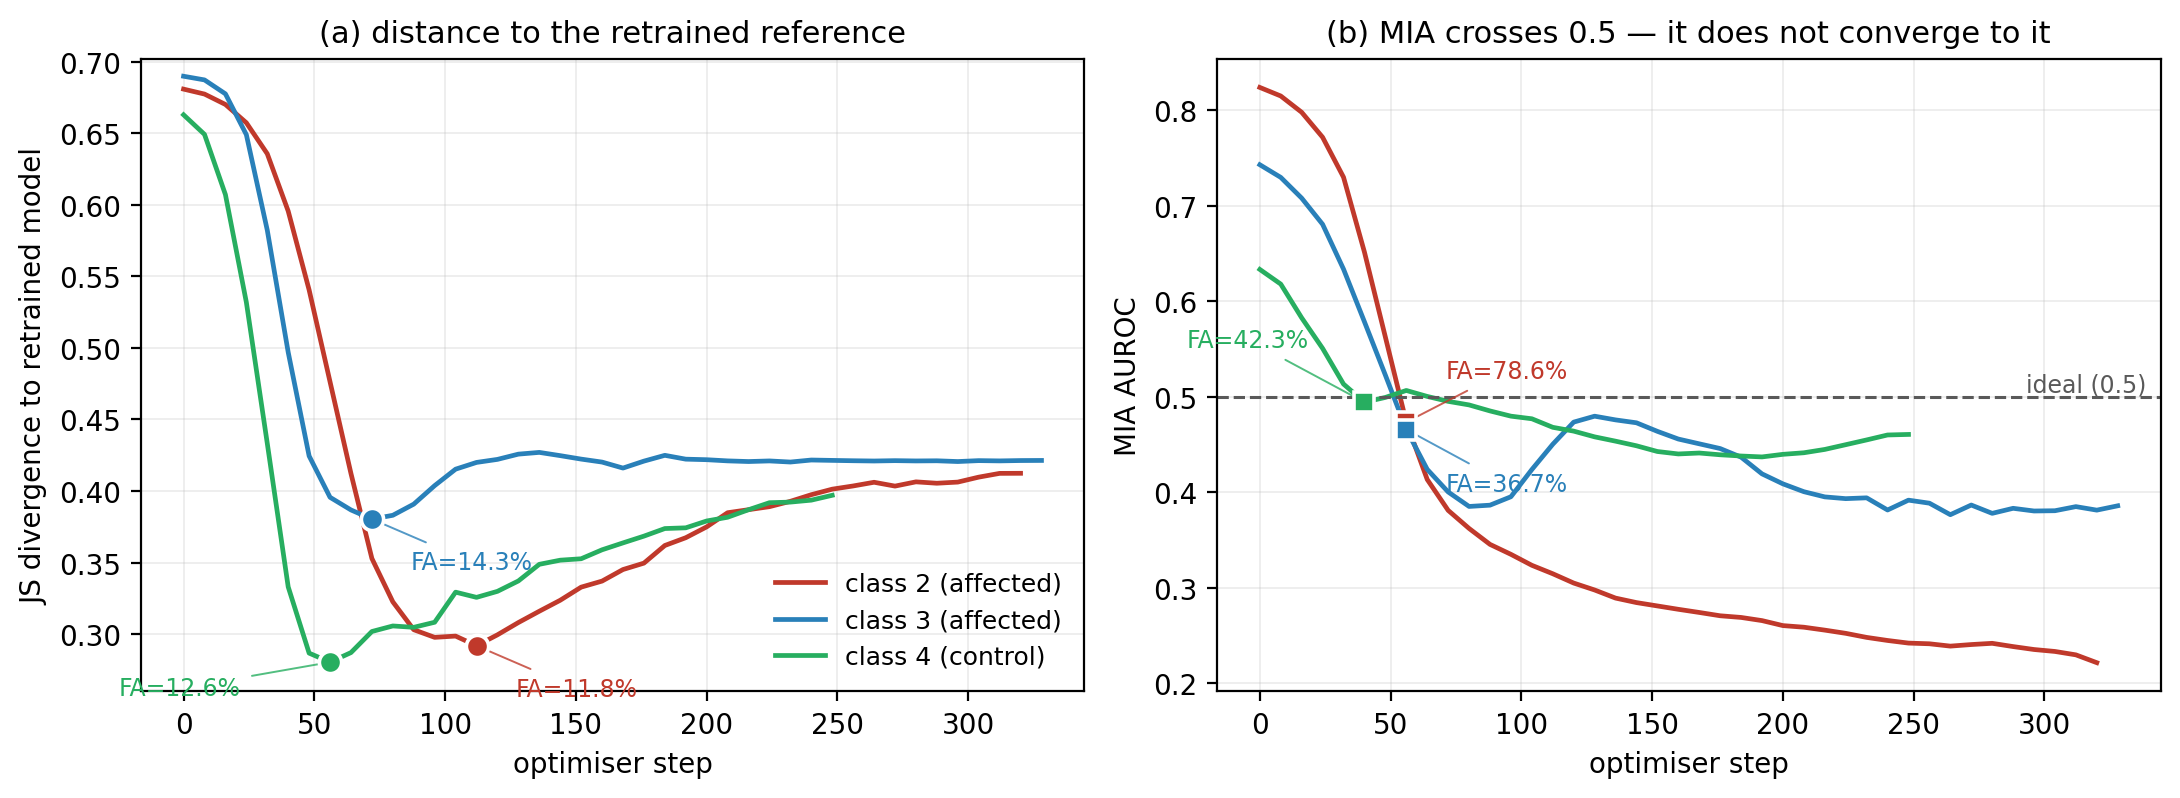
\includegraphics[width=\textwidth]{fig_trajectory.png}
\caption{\textbf{Unlearning overshoots the model it is trying to imitate, and
MIA cannot detect it.} \textbf{(a)}~Jensen--Shannon divergence to a
retrained-from-scratch reference along the unlearning trajectory. The curve is
U-shaped: the model first moves toward the reference, attains a minimum, then
moves away. Markers give the minimum, annotated with the forget accuracy there
($11.8$--$14.3\%$)---\emph{above} the $11.1\%$ chance level, whereas dual
stopping halts at ${\approx}7\%$. \textbf{(b)}~MIA AUROC on the same axis. It
sweeps \emph{through} the ideal $0.5$ rather than converging to it, so
$|\mathrm{MIA}-0.5|$ is minimised at the crossing. On class~2 that crossing
occurs while the model still classifies $78.6\%$ of the forget set
correctly.}
\label{fig:trajectory}
\end{figure}

\paragraph{The minimum is interior, and the current rule is past it.}
Divergence to the reference falls from $0.66$--$0.69$ at initialisation to
$0.28$--$0.38$, then rises again to $0.40$--$0.42$. So unlearning genuinely
moves the model toward a retrained one before moving away: over-forgetting is
not a metric artefact but a real overshoot in function space. The minimum lies
at $\mathrm{FA} = 11.8\%$, $14.3\%$ and $12.6\%$ for the three classes, while
dual stopping halts at ${\approx}7\%$ (\S\ref{sec:overforget}) --- past the
optimum in every case. Stopping at the minimum instead is close to free: test
accuracy changes by $-0.06$, $-0.03$ and $+0.79$pp and retain accuracy by
$+0.06$, $+0.36$ and $+0.08$pp. On the same trajectory it reduces divergence by
$0.016$, $0.003$ and $0.007$, and reduces $|\mathrm{MIA}-0.5|$ by $0.017$ and
$0.015$ on the two affected classes while moving the control by $+0.006$. This
is the pattern the criterion of \S\ref{sec:overforget} failed to produce:
the affected classes improve and the control stays put.

\paragraph{But the optimum is shallow, so we do not propose a numeric target.}
The three minima fall within $2.5$pp of one another in forget accuracy, which
invites the conclusion that ``stop at $\mathrm{FA}\approx 13\%$'' is a
deployable rule. The basin does not support that reading. Taking every
checkpoint within $5\%$ of the minimum divergence, the corresponding forget
accuracy spans $10.2$--$26.3\%$, $3.5$--$36.7\%$ and $6.9$--$21.9\%$ on the
three classes---$3.5$--$36.7\%$ overall. The agreement between the three
\emph{argmin} values is therefore largely a coincidence of where the snapshots
happened to land, and a single tuned number would not transfer. What the data
does support is directional and, we think, more useful: the optimum sits
\emph{above} the chance level, and a rule that drives forget accuracy to or
below chance is on the wrong side of it.

\paragraph{$|\mathrm{MIA}-0.5|$ is not an optimisation target.}
Panel~(b) is the more consequential finding. MIA AUROC does not converge to
$0.5$; it \emph{passes through} it, falling from $0.82$, $0.74$ and $0.63$ at
initialisation to $0.22$, $0.39$ and $0.46$ at the end. Consequently
$|\mathrm{MIA}-0.5|$ is minimised wherever the trajectory happens to cross,
which carries no information about unlearning quality. On class~2 the crossing
occurs at $\mathrm{FA} = 78.6\%$: a model that has barely forgotten anything
attains a \emph{perfect} MIA score. The two criteria also disagree about where
to stop, and in opposite directions---the divergence minimum and the MIA
minimum are $56$ steps apart on class~2, $56$ steps apart the other way on
class~3, and $8$ steps apart on class~4.

This sharpens the observation of \S\ref{sec:experiments} that a pre-unlearning
model already scores MIA $=0.533$. That was a single point; here we see the
whole path, and it shows that MIA $\approx 0.5$ is attainable at almost any
stage of unlearning, including stages with no meaningful forgetting at all.
Reporting MIA alongside forget accuracy is therefore not merely advisable but
necessary, and \emph{optimising} $|\mathrm{MIA}-0.5|$---which a practitioner
reading ``ideal $=0.5$'' might reasonably attempt---selects an arbitrary point
on the trajectory.

\paragraph{What remains unresolved.}
Stopping at the divergence minimum reduces over-forgetting without eliminating
it: class~2 still attains MIA $=0.315$ there, far from $0.5$. Nor do we have a
deployable rule, since locating the minimum requires the retrained reference
that unlearning exists to avoid, and the basin is too flat for a fixed forget
accuracy to stand in for it. We report the diagnosis---the stopping rule halts
on the wrong side of a real optimum---and leave a practical criterion open.
Whether the effect holds beyond the three PathMNIST classes measured here is
also untested; the experiment costs one unlearning run plus one retrained
reference per class.

% ============================================================
\section{Limitations in Full}\label{app:limitations}

\paragraph{Compute scales with classes and with data scarcity, and we cannot
predict it.} At \rev{its 15-epoch cap} \ours{} leaves STL-10 at
FA~$=75.7\%$, and an earlier version of this paper reported that as a failure
mode of the hard constraint on small forget sets. That diagnosis was wrong in
its conclusion though right about its cause. With 500 training images per class
the forget set yields only 4 mini-batches per epoch, ${\sim}60$ update steps in
total, and every step conflicts with the retain gradient---so progress per step
is small and the budget expires before forgetting completes. At 60 epochs, over
the same three seeds \rev{and with a per-step check and a $1\%$ target}, FA falls
to $1.73 \pm \rev{0.95}\%$ with RA~$=98.87\%$ \rev{(with the default $10\%$
target a single 60-epoch run stops at $9.2\%$)}. CIFAR-100
behaves the same way for a different reason: its per-class forget sets are small
because there are a hundred of them, and at 60 epochs its nine-class mean falls
from $4.07\%$ to $1.27 \pm \rev{0.39}\%$, bringing the $1\%$ chance level inside one
standard deviation. Neither constraint was infeasible; both runs were truncated.

What survives as a limitation is that we cannot say in advance how much budget a
new dataset needs. The binding resource is optimiser steps rather than epochs or
examples, and \ours{} offers no way to predict the requirement beyond monitoring
forget accuracy and continuing until the tolerance is met. A practitioner
deploying on an unfamiliar dataset should expect to discover the budget
empirically, and should treat a shared epoch count copied from another dataset
as a likely under-estimate.


\paragraph{Sample-level forgetting works, but at a cost the method cannot
control.} Every result in this paper removes a whole class. We tested the other
standard request type---forgetting a random subset of training points---on
CIFAR-10 at $1\%$ and $5\%$ of the training set, and report it as a scope limit
rather than a capability.

Two things go wrong, and they are different in kind. First, the forget objective
degenerates. \klr{} draws its power from the forget class being \emph{absent}
from the retain set, which drives $p_r$'s mass on that class to ${\sim}0$
(measured: $0.0002$); when the forget set is a random subset, the retain set
still covers every class and $p_r$ is uniform to three decimals
($0.100,0.100,\dots$). \klr{} therefore reduces exactly to
\texttt{kl\_uniform} in this regime, and the target carries no information about
\emph{which} points to forget. Second, dual stopping does not fire: the retain
budget is multiplicative on an initial retain loss of $0.0018$, so even at
$\alpha = 100$ both stopping-armed runs halted on the budget with forget accuracy
still at ${\sim}99.5\%$. A multiplicative budget is the wrong instrument against
a converged model; an absolute floor would be the right one.

Given a fixed 60-epoch budget and no stopping, forgetting does occur---forget
accuracy falls to $58.4\%$ at $1\%$ and $71.8\%$ at $5\%$---but
indiscriminately: retain accuracy falls from ${\sim}100\%$ to $73.2\%$ and test
accuracy to $71.9\%$, and forget accuracy ends \emph{below} test accuracy, which
is over-forgetting by the standard for this setting (a correctly unlearned point
should look like an unseen point of the same class, i.e.\ $\mathrm{FA}\approx
\mathrm{TA}$). The method has no mechanism to stop at that crossing.

The one clearly positive finding is the ablation. Removing the projection at
equal budget collapses the model completely: retain accuracy $14.2\%$ versus
$73.2\%$ with it, and test accuracy $17.1\%$ versus $71.9\%$---a $59$pp and
$55$pp difference respectively, far larger than the projection's effect in the
class-level ablation of Table~\ref{tab:ablation}. When forget and retain
gradients are drawn from the same distribution the conflict is near-total (the
projection fires on $100\%$ of steps), and the retain constraint is the only
thing keeping the model intact. The guarantee is therefore \emph{more}
load-bearing here, not less---which is why we regard sample-level forgetting as
a direction the constraint supports and the objective does not yet.

\paragraph{Mini-batch scope of the guarantee.} Theorem~\ref{thm:retain_safety}
bounds the \emph{sampled} retain objective---the quantity \ours{} projects
against---not the full-population retain loss. A population-exact per-step
guarantee would require controlling the gradient-variance term and is future
work.

\paragraph{The comparison with the closest prior work is structural, not
empirical.} Our separation from soft conflict-resolution methods
\citep{patel2025learning} rests on Theorem~\ref{thm:separation}(iv) and
Table~\ref{tab:properties}, both of which argue from the definition of the
update rule. We have not reimplemented that method and run it on our stack, so
we make no claim about how the two compare on accuracy, forgetting, or MIA. A
like-for-like empirical comparison is the most important piece of missing
evidence in this paper. Two related experiments are reported and should not be
mistaken for it: the projection-only ablation, isolating the projection from
\ours{}'s other three components (Table~\ref{tab:cifar10}), and the
projection-strength sweep, which interpolates our own update between a soft
penalty and the hard constraint (\S\ref{sec:strength}). Both test the mechanism;
neither runs the cited method.

\paragraph{Floating-point exactness.} The guarantee holds to float32 precision
(\S\ref{sec:alignment}); exact arithmetic would require float64 inner products.

\added{\paragraph{BatchNorm robustness is bought with compute, and is scoped.}
BN-robust \ours{} (\S\ref{sec:bn_robust}) survives the recalibration attack at
about seven times the wall-clock of the default configuration, because forgetting
that has to happen in the weights takes more steps. It was evaluated on two
datasets, CIFAR-10 (every class) and MNIST, and on base models that differ from
those behind the rest of the paper. It also defends only the normalisation
statistics: an attacker who modifies weights, as in the fine-tuning recovery
below, is outside what it changes.}

\paragraph{\rev{Sequential unlearning and fine-tuning recovery.}}
\rev{\emph{Sequential unlearning}: forgetting classes $0$, then $1$, then $2$
from each resulting checkpoint takes test accuracy $86.1 \to 76.8 \to 69.1$ and
retain accuracy $100.0 \to 89.7 \to 80.7$, with forget accuracy on the newest
class at most $2.7\%$. The decline is what forgetting does to these metrics,
not damage. TA counts every forgotten class's test images as errors, so fully
forgotten classes alone take it to $0.9$, $0.8$ and $0.7$ times the
retained-class accuracy (with the base model's $95.5\%$: $86.0$, $76.4$ and
$66.9\%$); RA is measured on a retain set that still contains the
earlier-forgotten classes, so fully forgotten classes take it to at most $8/9$
and $7/9$ ($88.9\%$ and $77.8\%$). The observed values sit at or above these
levels, so the retained classes are not damaged cumulatively. They sit above
them because earlier-forgotten classes partly return: an RA of $80.7\%$ requires
the two earlier classes to average at least $13\%$ training accuracy, above the
$10\%$ chance level. A sequential deployment should therefore re-check every
forgotten class after each request.} \emph{Fine-tuning recovery}: retraining the unlearned model on
$50$ forget-class samples raises forget accuracy from $1.9\%$ to $7.1\%$ after
five epochs and $51.3\%$ after ten---though by then the model is no longer
usable ($\mathrm{TA} = 34.6\%$, $\mathrm{RA} = 47.9\%$), so the attack recovers
the class only by destroying the model it attacks. \ours{} also does not provide
formal $(\varepsilon,\delta)$-DP guarantees.

\section{Per-Class Results}\label{app:perclass}

The main text reports per-dataset aggregates (Table~\ref{tab:cross}). Because a
mean over classes can conceal a method that succeeds on easy classes and fails on
hard ones, we report every class individually. Each row is the mean $\pm$
standard deviation over seeds $\{42,123,456\}$. CIFAR-100 per-class results
appear in the main text (Table~\ref{tab:cifar100}); the raw per-run CSVs for all
75 runs are released with the code.

\begin{figure}[t]
\centering
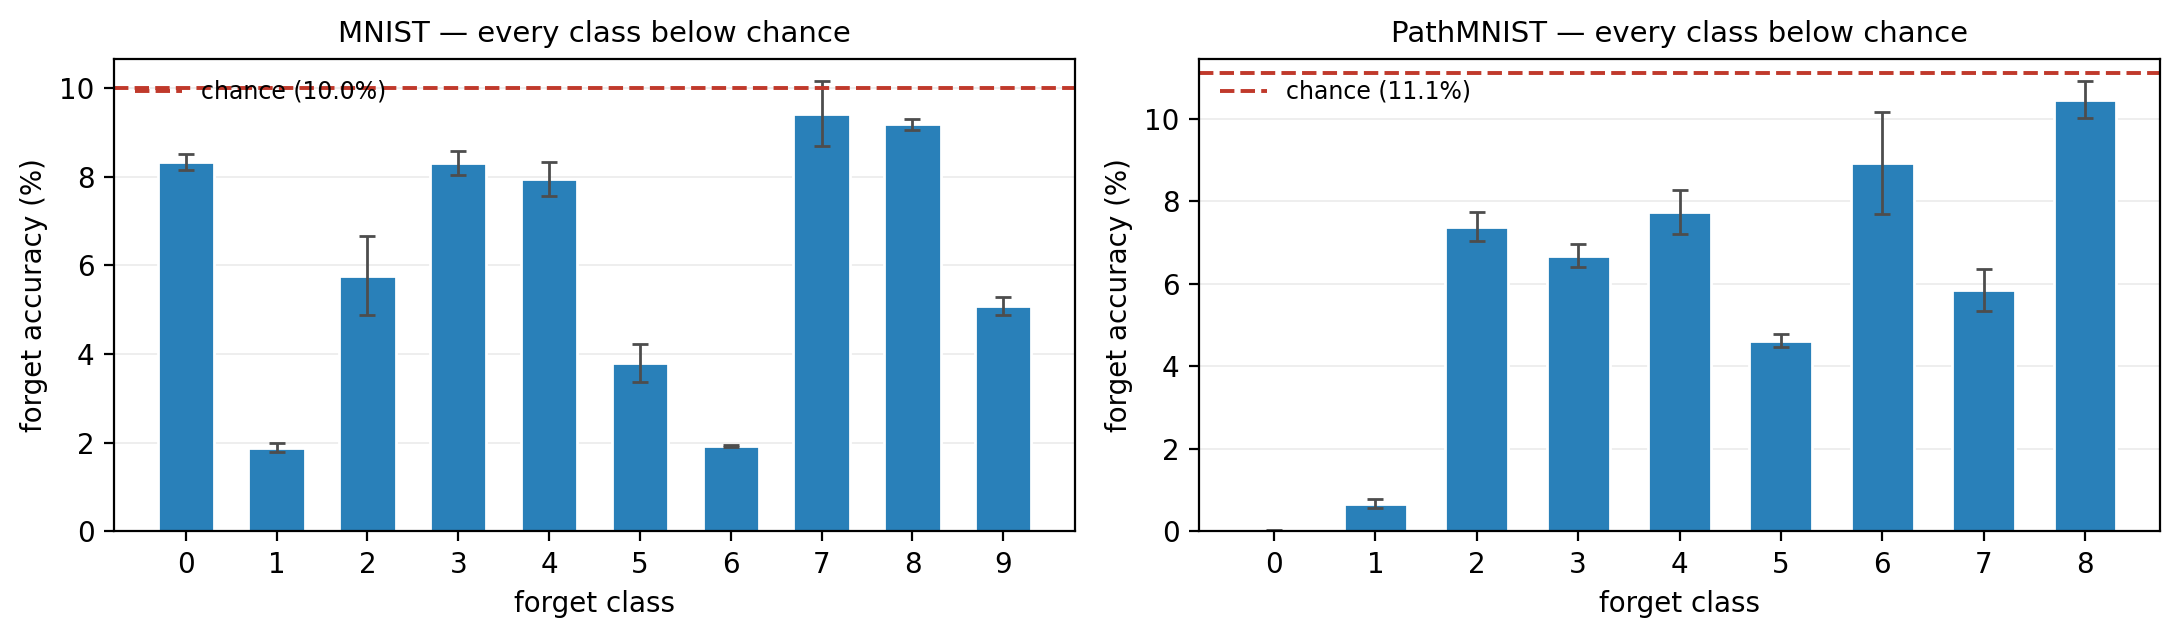
\includegraphics[width=\textwidth]{fig_perclass.png}
\caption{\textbf{Per-class forget accuracy} (mean $\pm$ std over three seeds).
Every MNIST and PathMNIST class individually falls below its chance level, so
the per-dataset means of Table~\ref{tab:cross} are not concealing a class that
fails.}
\label{fig:perclass}
\end{figure}

\subsection{MNIST (all 10 classes)}

Table~\ref{tab:app_mnist} gives all ten MNIST classes. Every class individually
falls below the $10\%$ chance level, with per-class mean FA ranging from
$1.89\%$ (class~1) to $9.42\%$ (class~7); the aggregate is therefore not
concealing a failure. Retain accuracy is essentially constant across classes
($99.42$--$99.54\%$), and MIA stays within $0.017$ of the ideal $0.5$ for every
class. Seed variance is small throughout (the largest FA standard deviation
across classes is $0.89$pp), indicating the procedure is stable rather than
seed-lucky.

\begin{table}[t]
\centering
\caption{\textbf{MNIST per-class forgetting} (mean $\pm$ std over 3 seeds).
Chance level is $10.0\%$; every class attains FA below it. TA is measured on the
full test set, so it necessarily drops by ${\sim}10$pp relative to the
$99\%$ base model once the forget class is correctly no longer recognised.}
\label{tab:app_mnist}
\begin{tabular}{@{}ccccc@{}}
\toprule
Forget class & TA (\%) & FA (\%)$\downarrow$ & RA (\%) & MIA \\
\midrule
0 & $90.26 \pm 0.05$ & $8.33 \pm 0.18$ & $99.42 \pm 0.00$ & $0.495 \pm 0.002$ \\
1 & $88.29 \pm 0.01$ & $1.89 \pm 0.09$ & $99.50 \pm 0.02$ & $0.512 \pm 0.001$ \\
2 & $89.68 \pm 0.07$ & $5.77 \pm 0.89$ & $99.51 \pm 0.01$ & $0.491 \pm 0.001$ \\
3 & $90.37 \pm 0.02$ & $8.31 \pm 0.27$ & $99.45 \pm 0.01$ & $0.483 \pm 0.001$ \\
4 & $90.22 \pm 0.01$ & $7.95 \pm 0.39$ & $99.43 \pm 0.02$ & $0.510 \pm 0.001$ \\
5 & $90.76 \pm 0.04$ & $3.80 \pm 0.43$ & $99.52 \pm 0.03$ & $0.499 \pm 0.001$ \\
6 & $90.08 \pm 0.02$ & $1.92 \pm 0.03$ & $99.50 \pm 0.02$ & $0.501 \pm 0.001$ \\
7 & $90.03 \pm 0.03$ & $9.42 \pm 0.74$ & $99.51 \pm 0.01$ & $0.490 \pm 0.000$ \\
8 & $90.36 \pm 0.03$ & $9.19 \pm 0.13$ & $99.50 \pm 0.02$ & $0.486 \pm 0.001$ \\
9 & $89.97 \pm 0.05$ & $5.09 \pm 0.21$ & $99.54 \pm 0.02$ & $0.503 \pm 0.000$ \\
\midrule
\textbf{Mean} & $\mathbf{90.00}$ & $\mathbf{6.17}$ & $\mathbf{99.49}$ & $\mathbf{0.497}$ \\
\bottomrule
\end{tabular}
\end{table}

\subsection{PathMNIST (all 9 classes)}

Table~\ref{tab:app_pathmnist} gives all nine PathMNIST tissue classes. Every
class again falls below the $11.1\%$ chance level, from $0.02\%$ (class~0) to
$10.46\%$ (class~8). Two observations deserve stating explicitly rather than
being averaged away.

First, the spread is far wider than on MNIST---per-class TA ranges from
$73.23\%$ to $89.28\%$---reflecting genuinely unequal class difficulty in
histopathology rather than instability: within-class seed variance remains small
(largest FA standard deviation $1.23$pp).

Second, and more importantly, \textbf{MIA AUROC is not uniformly near $0.5$}:
class~2 reaches $0.298$ and class~3 $0.388$, both well \emph{below} the ideal.
A value substantially below $0.5$ indicates that forget-class training samples
have become \emph{harder} to classify than forget-class test samples---the
signature of \emph{over}-forgetting, in which the unlearned model is
distinguishable from a retrained one in the opposite direction to a privacy
leak. It is detectable precisely because we report MIA per class and treat
distance from $0.5$ in either direction as a defect. We flag this as a real
limitation of the current stopping rule on PathMNIST: dual stopping targets FA,
which does not constrain how far past the retrained model's output statistics the
optimiser travels.

\begin{table}[t]
\centering
\caption{\textbf{PathMNIST per-class forgetting} (mean $\pm$ std over 3 seeds).
Chance level is $11.1\%$; every class attains FA below it. $^{\dagger}$Classes~2
and~3 show MIA well below the ideal $0.5$, indicating over-forgetting (see
text).}
\label{tab:app_pathmnist}
\begin{tabular}{@{}ccccc@{}}
\toprule
Forget class & TA (\%) & FA (\%)$\downarrow$ & RA (\%) & MIA \\
\midrule
0 & $73.23 \pm 0.06$ & $0.02 \pm 0.02$ & $99.01 \pm 0.01$ & $0.511 \pm 0.003$ \\
1 & $78.66 \pm 0.26$ & $0.68 \pm 0.12$ & $98.48 \pm 0.08$ & $0.473 \pm 0.003$ \\
2$^{\dagger}$ & $89.28 \pm 0.12$ & $7.38 \pm 0.35$ & $99.02 \pm 0.02$ & $0.298 \pm 0.003$ \\
3$^{\dagger}$ & $82.40 \pm 0.12$ & $6.68 \pm 0.28$ & $98.86 \pm 0.02$ & $0.388 \pm 0.005$ \\
4 & $78.04 \pm 0.08$ & $7.73 \pm 0.53$ & $98.95 \pm 0.03$ & $0.502 \pm 0.001$ \\
5 & $84.58 \pm 0.03$ & $4.62 \pm 0.15$ & $98.32 \pm 0.02$ & $0.548 \pm 0.001$ \\
6 & $78.58 \pm 0.25$ & $8.93 \pm 1.23$ & $98.77 \pm 0.06$ & $0.541 \pm 0.001$ \\
7 & $88.48 \pm 0.14$ & $5.85 \pm 0.50$ & $99.25 \pm 0.01$ & $0.562 \pm 0.001$ \\
8 & $75.36 \pm 0.04$ & $10.46 \pm 0.45$ & $99.28 \pm 0.03$ & $0.525 \pm 0.001$ \\
\midrule
\textbf{Mean} & $\mathbf{80.96}$ & $\mathbf{5.82}$ & $\mathbf{98.88}$ & $\mathbf{0.483}$ \\
\bottomrule
\end{tabular}
\end{table}

\paragraph{On the per-dataset MIA aggregate.}
The PathMNIST aggregate of $0.483 \pm 0.084$ in Table~\ref{tab:cross} is within
$0.017$ of ideal, but its standard deviation is an order of magnitude larger
than any other dataset's precisely because of classes~2 and~3. The aggregate is
accurate but uninformative here; this is a concrete instance of the more general
point of \S\ref{sec:experiments} that MIA must be read alongside FA, and
per-class rather than only in aggregate.

\begingroup\color{revised}% ---- new appendix subsection: added up to \endgroup
\subsection{BN-robust \ours{} on all ten CIFAR-10 classes}\label{app:bnrobust_perclass}

Table~\ref{tab:app_bnrobust} gives every CIFAR-10 class under the recalibration
attack of \S\ref{sec:bn_robust}, one seed per class (class~0 has three seeds in
Table~\ref{tab:bnrobust}). ``Pre'' and ``post'' are FA under test-time transforms
before and after \texttt{update\_bn} on the retain set. All runs share the
$93.97\%$ base of \S\ref{sec:bn_robust}. The calibrated runs here read the
stopping FA on the full retain set rather than the $10{,}240$-image subset; on
class~0 the two made identical stopping decisions (\S\ref{sec:bn_robust}).

\begin{table}[t]
\centering\color{revised}
\caption{\added{\textbf{BN-robust \ours{} per class} (CIFAR-10, seed~$42$). The
frozen-statistics configuration is recovered on every class. BN-robust is not,
under either stopping rule, and with calibrated stopping every class ships within
three standard errors of chance ($11.3\%$). Epochs ``$25{\to}22$'': the run
reached the cap and its best epoch was shipped.}}
\label{tab:app_bnrobust}
\small
\setlength{\tabcolsep}{4pt}
\begin{tabular}{@{}cccccccccc@{}}
\toprule
& \multicolumn{2}{c}{Frozen} & \multicolumn{2}{c}{BN-robust, naive}
& \multicolumn{5}{c}{BN-robust, calibrated} \\
\cmidrule(lr){2-3}\cmidrule(lr){4-5}\cmidrule(l){6-10}
Class & pre & post & pre & post & pre & post & epochs & TA & RA \\
\midrule
0 & $8.76$ & $99.22$ & $9.24$ & $9.28$ & $9.22$ & $9.24$ & 13 & $84.35$ & $95.60$ \\
1 & $2.40$ & $97.60$ & $10.66$ & $10.66$ & $6.66$ & $6.66$ & 8 & $84.56$ & $96.19$ \\
2 & $6.52$ & $98.30$ & $11.18$ & $11.16$ & $9.90$ & $9.92$ & 15 & $85.07$ & $95.27$ \\
3 & $4.78$ & $94.82$ & $11.30$ & $11.30$ & $10.00$ & $9.98$ & 16 & $85.92$ & $96.26$ \\
4 & $4.84$ & $97.34$ & $13.32$ & $13.34$ & $10.18$ & $10.16$ & $25{\to}22$ & $84.88$ & $94.74$ \\
5 & $7.28$ & $94.70$ & $8.78$ & $8.78$ & $9.40$ & $9.42$ & 12 & $84.52$ & $94.64$ \\
6 & $9.18$ & $99.14$ & $7.20$ & $7.20$ & $7.30$ & $7.30$ & 8 & $83.32$ & $94.41$ \\
7 & $3.38$ & $96.20$ & $11.36$ & $11.34$ & $9.12$ & $9.12$ & 10 & $84.49$ & $95.24$ \\
8 & $4.54$ & $99.26$ & $16.74$ & $16.68$ & $9.74$ & $9.68$ & 14 & $83.59$ & $94.67$ \\
9 & $2.52$ & $98.16$ & $15.44$ & $15.42$ & $8.92$ & $8.92$ & 11 & $83.84$ & $95.01$ \\
\midrule
Mean & $5.42$ & $97.47$ & $11.52$ & $11.52$ & $9.04$ & $9.04$ & --- & $84.45$ & $95.20$ \\
\bottomrule
\end{tabular}
\end{table}

\begin{figure}[t]
\centering\color{revised}
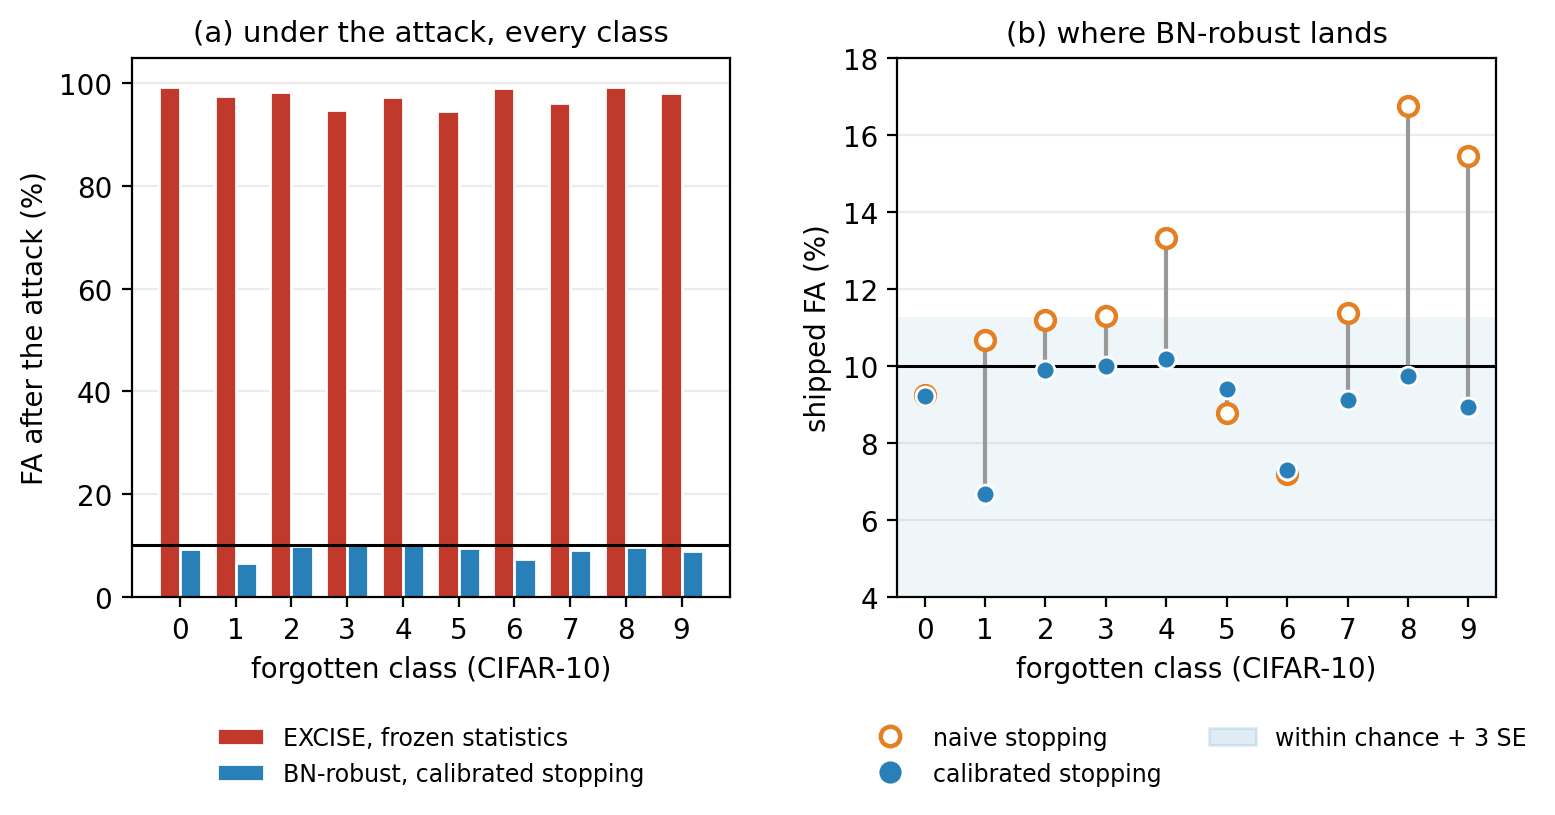
\includegraphics[width=\textwidth]{fig_bnrobust_perclass.png}
\caption{\added{\textbf{BN-robust on all ten CIFAR-10 classes} (seed~$42$; the data of
Table~\ref{tab:app_bnrobust}). (a)~Under the attack, the frozen-statistics
configuration is recovered on every class and BN-robust on none. (b)~Where
BN-robust ships: with naive stopping (open) five classes land above chance
$+\,3$\,SE; with calibrated stopping (filled), none do.}}
\label{fig:app_bnrobust}
\end{figure}
\endgroup% ---- end of the added appendix subsection

% ------------------------------------------------------------
\section{Hyperparameter Configuration}\label{app:hyper}

Table~\ref{tab:app_shared} lists the settings shared across all datasets and
Table~\ref{tab:app_perdataset} the per-dataset settings. All are released as YAML
configuration files; the reported runs use them unmodified.

\begin{table}[t]
\centering
\caption{\textbf{Shared hyperparameters} (identical for all six datasets). The
two components removed from \ours{} are listed explicitly with value $0$, since
they remain available as flags for the ablation of \S\ref{sec:ablation}.}
\label{tab:app_shared}
\begin{tabular}{@{}llll@{}}
\toprule
Symbol & Flag & Value & Role \\
\midrule
$\mu$ & \texttt{--momentum} & $0.9$ & momentum; projection applied \emph{after} accumulation \\
$c$ & \texttt{--max\_grad\_norm} & $1.0$ & clip on $d_t$, \emph{before} accumulation \\
$\lambda_{\mathrm{wd}}$ & \texttt{--weight\_decay} & $5\times10^{-4}$ & weight decay, applied inside $d_t$ \\
$T_{\mathrm{KD}}$ & \texttt{--temperature} & $4.0$ & distillation temperature \\
--- & \texttt{--forget\_objective} & \klr{} & KL toward retain-confusion $p_r$ \\
--- & \texttt{--batch\_size} & $128$ & forget and retain mini-batch size \\
--- & \texttt{--fa\_check\_freq} & $50$ & intra-epoch FA check interval (batches) \\
--- & \texttt{--seed} & $\{42,123,456\}$ & three seeds per task \\
\midrule
\multicolumn{4}{@{}l}{\emph{Removed components (retained as ablation flags only)}} \\
$\lambda$ & \texttt{--rep\_weight} & $0.0$ & representation erasure (removed) \\
$\gamma$ & \texttt{--forget\_gate} & $0.0$ & entropy gate (removed) \\
\bottomrule
\end{tabular}
\end{table}

\begin{table}[t]
\centering
\caption{\textbf{Per-dataset hyperparameters.} $K$ is the number of classes.
Note that the forget-accuracy target $\tau_F$ is set to the chance level
$100/K$ for every dataset---it is not tuned per dataset, but derived from the
task.}
\label{tab:app_perdataset}
\begin{tabular}{@{}lcccccc@{}}
\toprule
Dataset & $K$ & Epochs $T$ & $\eta$ & $\beta$ (KD) & $\alpha$ (retain budget) & $\tau_F = 100/K$ \\
\midrule
CIFAR-10  & 10  & 15 & $5\times10^{-4}$ & $2.0$ & $5.0$ & $10.0\%$ \\
CIFAR-100 & 100 & 20 & $5\times10^{-4}$ & $2.0$ & $5.0$ & $\phantom{0}1.0\%$ \\
MNIST     & 10  & 12 & $2\times10^{-4}$ & $3.0$ & $4.0$ & $10.0\%$ \\
SVHN      & 10  & 15 & $2\times10^{-4}$ & $3.0$ & $5.0$ & $10.0\%$ \\
STL-10    & 10  & 15 & $2\times10^{-4}$ & $5.0$ & $5.0$ & $10.0\%$ \\
PathMNIST & \phantom{0}9 & 12 & $2\times10^{-4}$ & $5.0$ & $4.0$ & $11.1\%$ \\
\bottomrule
\end{tabular}
\end{table}

\paragraph{Tuning effort.}
Only four quantities vary across datasets: the epoch cap $T$, the learning rate
$\eta$, the KD weight $\beta$, and the retain budget $\alpha$. The learning rate
takes one of two values ($5\times10^{-4}$ for the CIFAR datasets,
$2\times10^{-4}$ elsewhere), $\beta$ one of three, and $\alpha$ one of two. The
forget target $\tau_F$ is not tuned at all: it is fixed to the chance level
$100/K$ implied by the task. Notably, $\mu$, $c$, $\lambda_{\mathrm{wd}}$, and
$T_{\mathrm{KD}}$---the four quantities that enter the guarantee of
Theorem~\ref{thm:app_main}---are held constant across all six datasets, so the
bound $\tfrac12 L\eta^2(c/(1-\mu))^2$ varies across datasets only through
$\eta$ (and through the dataset-dependent smoothness constant $L$).

\paragraph{A note on defaults.}
The command-line default for \texttt{--max\_grad\_norm} in the released code is
$5.0$, whereas every configuration file sets $c=1.0$. Runs launched without
\texttt{--config} would therefore use a different clip threshold, and a
correspondingly weaker constant in
(\ref{eq:app_c}). All results in this paper use the configuration files. We note
this because the value of $c$ enters the guarantee directly, so it should not be
inherited silently from a default.

% ------------------------------------------------------------
\section{Distance to the Retrained Model: A Refuted Hypothesis}\label{app:d2r}

This appendix reports a negative result. We formed a hypothesis about why
\ours{} over-forgets on two PathMNIST classes, derived a deployable fix from it,
pre-committed to a falsifiable prediction, ran the experiment, and the
prediction did not hold. We report it in full because the experiment also
produced the diagnosis that we believe is correct, and because the refuted
hypothesis concerns \ours{}'s own forget objective.

\subsection{The defect, and the hypothesis}

Per-class reporting (Appendix~\ref{app:perclass}) showed that on PathMNIST
classes~2 and~3, MIA AUROC reaches $0.298$ and $0.388$---far \emph{below} the
ideal $0.5$. Forget accuracy is satisfied on both, so FA alone certifies these
runs as successes when they are not. A value below $0.5$ means forget-class
training samples have become \emph{harder} to classify than forget-class test
samples: the model is still distinguishable from a retrained one, in the
opposite direction to a privacy leak.

\rev{An earlier version of our forget-side condition (Eq.~\ref{eq:problem}) was
$\KL(p_\theta(x_f)\,\|\,p_r) \le \epsilon$}, a statement about
\emph{distributions}, but dual stopping (\S\ref{sec:stopping}) implements
\rev{$\mathrm{FA} \le \tau_F$}, a statement about \emph{argmax}. These are not
equivalent, and we hypothesised that the discrepancy was the cause: FA cannot
distinguish (a)~$p_\theta(x_f)$ having moved \emph{to} the distribution a
retrained model produces from (b)~having moved \emph{past} it, since both give
$\mathrm{FA}\approx 0$.

The hypothesised fix was to enforce the constraint as stated. Since $p_r$ is
computed from the \emph{original} model, this needs no retrained reference and
is deployable: stop on $\KL(p_\theta(x_f)\|p_r)$ rather than on FA. We reasoned
that this quantity is minimised at $p_\theta = p_r$ and rises on either side, so
a stop-when-it-stops-improving rule would halt at the minimum---exactly the
point FA cannot locate.

\paragraph{Prediction (pre-committed).} Replacing FA stopping with KL stopping
would, on the affected classes, (1)~reduce $|\mathrm{MIA}-0.5|$, (2)~reduce
Jensen--Shannon divergence to a retrained reference, and (3)~not materially
worsen FA or RA, while leaving an unaffected control class approximately
unchanged.

\subsection{Design}

We retrained reference models without the forget class for PathMNIST classes~2
and~3 (affected) and class~4 (control, MIA already $0.501$), keeping all $K$
output heads so that output distributions remain comparable, and training all
three identically for a fixed 30-epoch cosine schedule so that no reference is
better converged than another. Arm~A is \ours{} with FA stopping (the deployed
configuration); arm~B disables FA stopping and enables KL stopping. Oracle
metrics are computed against the references: JS divergence between output
distributions on the forget set (primary), top-1 agreement with the reference,
Fr\'echet distance between penultimate features, and MIA.

The control class is the load-bearing part of the design: a criterion that
merely stops earlier everywhere would improve the affected classes while also
perturbing the control, whereas a targeted fix should leave the control alone.

\subsection{Result: the prediction fails}

Table~\ref{tab:app_klstop} reports the outcome. Across three classes and four
metrics, arm~B is better on 2 comparisons and worse on 10. The primary oracle
metric---JS divergence to the retrained model---is \emph{worse in all three
classes}. The control class degrades on every metric, which is precisely the
signature that rules out a targeted fix. Only class~3 improves on
$|\mathrm{MIA}-0.5|$.

\begin{table}[t]
\centering
\caption{\textbf{KL stopping vs.\ FA stopping on PathMNIST}, measured against
retrained references. Arrows mark the direction of improvement. The prediction
was that the affected classes would improve and the control would not move;
neither held.}
\label{tab:app_klstop}
\begin{tabular}{@{}llccccc@{}}
\toprule
Class & Arm & $|\mathrm{MIA}{-}0.5|\downarrow$ & JS$\downarrow$ &
agree \%$\uparrow$ & Fr\'echet$\downarrow$ & $\KL$ to $p_r$ \\
\midrule
\multirow{2}{*}{2 (affected)}
 & FA stop & $0.205$ & $0.308$ & $45.4$ & $185.7$ & $0.957$ \\
 & KL stop & $0.268$ & $0.412$ & $23.5$ & $332.0$ & $0.052$ \\
\midrule
\multirow{2}{*}{3 (affected)}
 & FA stop & $0.115$ & $0.382$ & $31.2$ & $375.2$ & $0.805$ \\
 & KL stop & $\mathbf{0.068}$ & $0.421$ & $\mathbf{39.8}$ & $780.1$ & $0.002$ \\
\midrule
\multirow{2}{*}{4 (control)}
 & FA stop & $0.001$ & $0.286$ & $38.7$ & $141.1$ & $1.510$ \\
 & KL stop & $0.044$ & $0.399$ & $12.3$ & $297.7$ & $0.116$ \\
\bottomrule
\end{tabular}
\end{table}

\paragraph{The proxy is anti-correlated with the oracle.}
A proxy is only usable if it tracks the quantity it stands in for. Across the
six checkpoints, the rank correlation between $\KL(p_\theta\|p_r)$ and JS
divergence to the retrained model is $\rho = -1.00$ (Pearson $-0.94$): the
ordering is perfectly inverted. Driving the deployable proxy toward zero moves
the model monotonically \emph{away} from the retrained reference. This is the
opposite of the relationship the hypothesis required.

\subsection{Why it failed}

\paragraph{(i) The criterion never fired.}
In all three runs of arm~B the terminating condition was the retain-loss budget,
not the KL rule. The reason is visible in the logged trajectories:
$\KL(p_\theta(x_f)\|p_r)$ decreases essentially monotonically (class~2:
$5.53 \to 0.05$ over 8 checks with zero increases; class~4: $2.73 \to 0.07$,
zero increases; class~3: $2.06 \to 0.002$ over 20 checks with 4 small
increases). It never turns back up, so a stop-when-it-stops-improving rule
cannot trigger. The U-shape the hypothesis assumed does not exist over the
range the optimiser traverses.

This is also a limitation of the test, and we state it plainly: because the KL
rule never fired and FA stopping was disabled, arm~B is in effect \ours{}
\emph{without forget-side stopping} (FA reaches $0.0$ in all three runs), which
is closer to the $-$Stopping ablation than to a KL-stopped method. The
comparison in Table~\ref{tab:app_klstop} is therefore evidence against the
criterion \emph{as specified}, not a clean contrast between two stopping rules.

\paragraph{(ii) $p_r$ is a global average; a retrained model routes per-sample.}
$p_r$ is a single distribution, the retain-set average softmax, and it is the
same target for every forget sample. A retrained model does something different:
it routes each forget-class image to whichever surviving class that particular
image most resembles, giving an input-dependent output distribution. Matching
$p_r$ more closely therefore makes the model's predictions on forget data
unnaturally homogeneous across samples. The agreement column is the evidence:
as $\KL$ to $p_r$ falls by one to three orders of magnitude, top-1 agreement
with the reference \emph{collapses} on two of the three classes
($45.4 \to 23.5$ on class~2, $38.7 \to 12.3$ on class~4). If $p_r$ were the
right target, matching it better should have raised agreement. Class~3 moves the
other way ($31.2 \to 39.8$), so the effect is not universal.

\paragraph{Confound we cannot separate.}
$\KL$ to $p_r$ decreases with training time while JS to the reference increases
over the observed range, so the two are mechanically anti-correlated and the
$\rho = -1.00$ figure partly reflects run duration rather than target quality
alone. The agreement collapse is the part of the evidence that speaks to the
target itself, and it rests on two of three classes. We therefore claim the
criterion is refuted, and treat the mechanism as well-supported but not
established.

\subsection{What the experiment did establish}

\paragraph{The FA rule overshoots its own target.}
All three FA-stopped runs halt at $\mathrm{FA} \approx 7\%$ against a target of
$11.1\%$ (the chance level), overshooting by $3.9$--$4.2$pp, because the
intra-epoch FA check is evaluated only every 50 batches. The over-forgetting we
set out to explain is thus at least partly a \emph{granularity} defect in how
the existing criterion is enforced, not evidence that FA is the wrong quantity.

\paragraph{Less unlearning was better on every class.}
JS divergence to the retrained model is lower at the earlier stopping point in
all three classes. Over the range we observe, the model is still moving toward
the retrained reference when FA stopping halts it, and continues away from it
afterwards. Combined with the overshoot above, this points to stopping
\emph{earlier and more precisely} rather than to replacing the stopped quantity.

\paragraph{Consequence for the method.}
We draw a narrower conclusion about \klr{} than the original formulation
implies. As a forget-side \emph{direction}, $p_r$ is a better target than the
uniform distribution (\S\ref{sec:forget_obj}). As a \emph{target to be minimised
to zero}, it is actively harmful. \rev{Accordingly Eq.~\ref{eq:problem} states
the forget condition on forget accuracy and uses the divergence only as the
direction of the search}, and we do not claim $p_r$ is what a retrained model produces on forget
inputs---the measurements here show it is not.

\subsection{Open question}

Where JS divergence to the retrained model is minimised along the unlearning
trajectory remains unmeasured. Since JS is still falling when FA stopping fires
and rising afterwards, a minimum exists between the base model and the FA-stopped
point; locating it would establish whether a single FA level identifies it across
classes, which would make it deployable, or whether it varies per class, which
would not.
This question is answered in \S\ref{sec:trajectory}: the minimum is interior, lies above the chance level, and the current rule stops past it.

% ------------------------------------------------------------
\section{Ethical and Societal Considerations}\label{app:ethics}

\paragraph{Unlearning as evidence removal.}
A method that makes a model indistinguishable from one retrained without
specific data could be misused to destroy evidence that problematic data was
used for training. This is a dual-use property of the unlearning goal itself
rather than of \ours{} specifically, but \ours{} does make it concrete. Partial
mitigation is that \ours{} leaves an audit trail by construction: projection-rate
logs, the FA trajectory, and retain-loss budget history are all recorded per run,
so an auditor with access to the logs can establish that unlearning was applied
and to what extent. We note this is mitigation, not prevention---an adversary who
controls the logs controls the audit.

\paragraph{Selective fairness degradation.}
Class-level unlearning removes all samples of a class, which may correspond to a
demographic group. Crucially, the accuracy degradation we observe is
\emph{not} confined to the forgotten class: test accuracy falls beyond what the
removed class alone accounts for, and the per-class spread on PathMNIST
(Appendix~\ref{app:perclass}) shows the effect is uneven across classes.
Deployers should therefore monitor per-class accuracy before and after
unlearning rather than only aggregate accuracy, which can conceal a
disproportionate cost borne by one group.

\paragraph{Over-forgetting as a distinct harm.}
The PathMNIST finding (Appendix~\ref{app:perclass}) shows that a model can be
pushed \emph{past} the retrained reference. This matters ethically as well as
technically: such a model is still distinguishable from one trained without the
data, so a deletion request has not been faithfully honoured, yet every
FA-based check reports success. Compliance evidence resting on forget accuracy
alone would be misleading here.

\paragraph{Regulatory gap.}
Approximate unlearning methods, including \ours{}, do not satisfy formal
$(\varepsilon,\delta)$-differential-privacy certification. Whether
MIA AUROC~$\approx 0.5$ constitutes legally sufficient ``erasure'' under
instruments such as the GDPR right to erasure remains an open legal question on
which we take no position. The per-step guarantee of
Theorem~\ref{thm:retain_safety} is a statement about \emph{retain-side utility},
not a privacy certificate, and should not be presented as one.

% ------------------------------------------------------------
\section{Reproducibility}\label{app:repro}

\paragraph{Artefacts.}
Code, YAML configuration files, per-run summary CSVs for all 75 runs, and the
BatchNorm-recalibration diagnostic are released in the anonymised repository.
\todo{Insert the anonymised repository URL.}
The archived $\mu=0$ results underlying Table~\ref{tab:momentum} are released
alongside the main results, so the momentum ablation can be re-derived without
re-running it.

\paragraph{Environment.}
PyTorch $\ge 2.0$ with CUDA; ResNet-18 (11.7M parameters) throughout. Runs were
executed on a single GPU. Datasets download automatically except PathMNIST,
which is obtained through \texttt{medmnist}.

\paragraph{Implementation details that affect results.}
\begin{itemize}
\item Momentum and weight decay are applied \emph{manually} so that the
projection acts on the post-momentum update; the underlying \texttt{torch} SGD
object is configured with \texttt{momentum=0}, \texttt{weight\_decay=0} and acts
only as a plain step. Reading the optimiser construction alone is therefore
misleading---see \S\ref{sec:optimiser} and Appendix~\ref{app:setup}.
\item Clipping is applied to $d_t$ before momentum accumulation, and \emph{not}
to the final update. Reversing this changes the effective step size by a factor
$1/(1-\mu)$ (Proposition~\ref{prop:clip}).
\item The projected update is rescaled to the pre-projection norm.
\item BatchNorm layers are set to \texttt{eval()} immediately after the model is
set to \texttt{train()}, so running statistics are frozen during unlearning.
\added{BN-robust \ours{} (\S\ref{sec:bn_robust}) instead recomputes them from
$512$ retain images before every step (\texttt{--bn\_robust exact
--bn\_recal\_samples 512}) and on the full retain set under test-time transforms
after the last step. It reads the stopping forget accuracy under statistics
recomputed from $10{,}240$ retain images (\texttt{--bn\_calibrated\_stop
--bn\_stop\_recal\_samples 10240}), ships the best epoch when the target is not
met (\texttt{--restore\_best\_epoch}), and uses an epoch cap of $25$.}
\item The retain-confusion distribution $p_r$ is precomputed once from the frozen
original model.
\item Forward hooks are registered on \texttt{layer3}, \texttt{layer4}, and
\texttt{avgpool} for feature-level diagnostics.
\item Configuration files set $c=1.0$; the CLI default is $5.0$ (see above).
\item All baselines are re-run within the same codebase under a unified MIA
protocol, rather than quoted from their source papers.
\end{itemize}

\paragraph{Determinism and seeds.}
Every 10-class task is run with seeds $\{42,123,456\}$ and reported as
mean~$\pm$~std; CIFAR-100 uses a single seed per class. Seed variance is small
(Appendix~\ref{app:perclass}). As an internal consistency check, the two
ablation variants that are no-ops under the shipped configuration
(\texttt{--rep\_weight 0}, \texttt{--forget\_gate 0}, both already $0$) produce
byte-identical metrics, confirming both that the runs are deterministic given a
seed and that those components are genuinely inactive.

\paragraph{Known reproduction caveats.}
The floating-point exactness of the guarantee is precision-dependent
(Remark~\ref{rem:float}): reference implementations should accumulate the
projection inner products in float64. Wall-clock timings depend on the GPU and
on how early dual stopping fires, so step counts rather than seconds are the
portable quantity.

\end{document}
